% !TEX root = ../geom_autistic_intro.tex
\section{Principal and Associated Bundles}

    Now that we have comprehensively reviewed the fundamentals of Lie groups and their actions on manifolds, we are finally ready to return to Klein's Erlangen program as described at the beginning of Section~\ref{sec: Lie theory ii}.

    Principal bundles appeared in the last \sect\ as a natural special case of Lie group actions on manifolds. In this \sect, however, they will acquire a special elevated status in the theory of general fiber bundles. Recall that any fiber bundle that admits a $G$-atlas such that the structure group $G$ acts on the typical fiber $F$ faitfully is completely determined by the cocycle of its transition functions. This led to the equivalence of any two categories of fiber bundles $\FB^\sigma$ and $\FB^{\sigma'}$ for any two faithful $G$-actions $G\overset{\sigma}{\acts}F$ and $G\overset{\sigma'}{\acts}F'$ (see (\ref{eq equivalence of bundle categories})). This means that most functorial geometric structures on fiber bundles can be defined by providing their description on any one of these equivalent categories. The choice of the category of principal bundles is natural and convenient for two reasons. 
    
    On a fundamental level, principal $G$-bundles are exactly the $G$-bundles whose typical fiber is $G$ itself, and the action $\sigma$ is the action by translations (which is faithful indeed). The definition of this category, therefore, requires no additional information aside from the group $G$ itself. 
    
    On a more practical level, however, the particular convenience of working on principal bundles is due to the fact that Lie groups are parallelizable, so the tangent bundle of a principal $G$-bundle is significantly simpler than the tangent bundle of a generic bundle with structure group $G$. 

    For these reasons, while everything discussed in this \sect\ can equally well be introduced without any preference being given to principal bundles, we will usually start with them due to their unique convenience and simplicity of computations. In specific applications, principal bundles are almost never where the ``physical objects'' live, so this style of exposition should not be viewed as anything more than a slight of hand.



\subsection{Principal fiber bundles}\label{sec: principal bundles}


Recall that in Definition \ref{def pfb} we defined principal bundles as free and proper Lie group actions, and provided an equivalent characterization in terms of equivariant local trivializations. We now make the latter definition explicit.

\begin{defn}[Principal fiber bundle II]\index{Principal fiber bundle}\label{def pfb 2}
    Let $(P,G,\Phi)$ be a free Lie group action, let $M$ be a manifold and let $\pi:P\to M$ be a smooth mapping. The tuple $(P\overset{\pi}{\to}M,G,\Phi)$ is called a principal $G$-bundle if for every $m\in M$ there exists an open neighborhood $U_m$ of $m$ and a diffeomorphism $\chi:\pi^{-1}(U_m)\to U_m\times G$ such that
    \begin{enumerate}
        \item $\chi$ intertwines $\Phi$ with the $G$-action on $U\times G$ by translations of the second component (left if $\Phi$ is left, resp.\ right if it is right).
        \item $\pr_{U_m}\circ \chi=\pi$ on $\pi^{-1}(U_m)$.
    \end{enumerate}
    For brevity we will often denote principal bundles by $P(G,M)$.
\end{defn}

The existence of local trivializations implies that $\pi$ is a smooth submersion. The fibers of a surjective submersion are embedded submanifolds, all diffeomorphic to the structure group $G$. They are also the orbits of the $G$-action on $P$. Following convention, we will usually assume that $\Phi$ is a right action and call $P$ a \emph{right} principal $G$-bundle (not to be confused with the left $G$-action on the typical fiber).

\begin{rem}
    \begin{enumerate}
        \item Principal bundles can also be understood in terms of $G$-structures. Namely a $G$-bundle $(P\overset{\pi}{\to}M,G\acts F,\calG)$ is principal iff the action $G\acts F$ is free and transitive. 
        
        \item Recall that a $G$-invariant structure can be naturally lifted from the typical fiber to the fibers of the $G$-bundle itself. However, the Lie group structure of $G$ is not translation-invariant: e.g.\ the identity element is not invariant under translations. Therefore, \emph{the fibers of a \gls{pfb} do not carry a natural group structure}. In particular, unlike \glspl{vb}, they have no distinguished elements and therefore no analog of a zero section. Instead, the fibers are merely principal homogeneous spaces of $G$ (that is, $G\slash \{e\}$).

        \item Another feature that distinguishes \glspl{pfb} from all other $G$-bundles is that the typical fiber $G$ carries \emph{two} commuting actions of $G$. The bundle construction via transition functions has those functions act on $G$, say, from the left, which precludes the existence of any left $G$-action on the bundle itself (unless $G$ is abelian). However, the action of $G$ on itself by right translations is left untouched by the bundle construction, and this is the action with respect to which the trivializations are equivariant in the above definition. Even if $G$ is abelian, then the two actions coincide anyway, so there still won't be two actions on the bundle.
    \end{enumerate}
    Since all of these facts are easier to state explicitly in the definition of a principal bundle, Definition~\ref{def pfb 2} is the most common one in the literature.
\end{rem}




\begin{example}
    \begin{enumerate}
        \item $\pr_M:M\times G\to M$ with the right action of $G$ on the second factor is a trivial $G$-\gls{pfb}.
        \item The direct product $P_1\times P_2$ of two \glspl{pfb} with respective structure groups $G_1,G_2$ over bases $M_1$ and $M_2$, has a natural structure of a principal $G_1\times G_2$-bundle over $M_1\times M_2$.
        \item If $H\sub G$ is a closed subgroup, then $H$ acts on $G$ freely by right translation and this action is proper. Thus, $G\to G\slash H$ is a principal $H$-bundle.
    \end{enumerate}
\end{example}

\begin{prop}[{{\cite[Prop.~1.1.6]{RS2}}}]\label{prop 1.1.6 RS2}
    Local trivializations of a \gls{pfb} are in bijective correspondence with its local sections. In particular, a \gls{pfb} is trivial iff it admits a global section.
\end{prop}
\begin{proof}
    If $\chi:P\to M\times G$ is a global trivialization, then we set $s(m)=\chi^{-1}(m,e)$, where $e\in G$ is the identity. This is a smooth global section of $P$. Conversely, given a global section $s:M\to P$, for every point $p\in P$ there exists a unique group element $g(p)\in G$ such that $p=\Phi_{g(p)}(s(\pi(p)))$. This defines an equivariant smooth map $g:P\to G$, so that $g(\Phi_h(p))=g(p)h$. Thus $(M,\pi\times g)$ is a global trivialization.

    The statement for local sections follows by considering trivial restrictions of the bundle of the form $\restr{P}{U}$.
\end{proof}


\begin{rem}
    By the above proposition, specifying a bundle atlas $\{(U_\alpha,\chi_\alpha)\}$ for a \gls{pfb} $P\to M$ is equivalent to providing a collection of local sections $\{s_\alpha:U_\alpha\to P\}$. The relationship between the two is 
    \[s_\alpha(m)=\chi_\alpha^{-1}(m,e).\]
    According to (\ref{eq transition functions}), if the transition functions of $P$ are $g_{\beta\alpha}:U_{\alpha\beta}\to G$, then the transformation rule for these local sections, assuming a right \gls{pfb}, reads 
    \[s_\alpha(m)=s_\beta(m)\cdot g_{\beta\alpha}(m)\quad \text{for a right \gls{pfb}},\label{eq transf rule for sections}\]
    where on the right we're using the principal right action. Note that since the $G$-action on the typical fiber is always assumed to be a left one, transition functions in the case of a left principal $G$-bundle should be defined as $t_{\beta\alpha}(m,h)=(m,hg_{\beta\alpha}^{-1})$. This then leads to 
    \[s_\alpha(m)=g_{\alpha\beta}(m) \cdot s_\beta(m) \quad \text{for a left \gls{pfb}},\]
    and it is easy to see that this implies the regular cocycle condition $g_{\alpha\beta}g_{\beta\gamma}g_{\gamma\alpha}=e$.

    Since we will usually work with right principal bundles, we will identify the transition functions with $g_{\beta\alpha}$ and use only the symbol $t_{\beta\alpha}$ for them. To obtain the analogous statements for left principal bundles, one then needs to replace $t_{\beta\alpha}$ multiplying from the left by $t_{\alpha\beta}$ multiplying from the right.
\end{rem}

Now we need to specify the notion of morphism of \glspl{pfb}. Recall that a morphism between $G_1$- and $G_2$-structures is a bundle morphism whose fiberwise representatives lie in $G_1\times G_2$-orbits of some canonically chosen maps between the typical fibers (cf.\ Definition~\ref{def S-bundle}). Since the typical fibers of principal bundles are the Lie groups themselves, it is clear that these canonical maps should be chosen as Lie group homomorphisms. The $G_1\times G_2$-orbits of homomorphisms are exactly the sets of equivariant maps, as we now show. 

\begin{defn}[$\lambda$-equivariant map]
    Let $G_1\acts F_1$ and $G_2\acts F_2$ be two right Lie group actions and let $\lambda:G_1\to G_2$ be a Lie group homomorphism. A smooth map $\varphi:F_1\to F_2$ is called (right) $\lambda$-equivariant if $\varphi(f\cdot g_1)=\varphi(f)\cdot \lambda(g_1)$ for all $f\in F,g_1\in G_1$.
\end{defn}

\begin{prop}
    Let $\lambda:G\to G'$ be a Lie group homomorphism and let $G,G'$ act on themselves by right translations. Then a smooth map $\varphi:G\to G'$ is right $\lambda$-equivariant iff it has the form $\varphi(g)=g'\lambda(g)$ for some $g'\in G'$.
\end{prop}
\begin{proof}
    Let $\varphi$ be right $\lambda$-equivariant. Then
    $\varphi(g)=\varphi(e\cdot g)=\varphi(e)\lambda(g)$,
    so setting $g'=\varphi(e)$ proves the assertion. The other direction is obvious.
\end{proof}


Recall that the maps $\Phi_{\alpha a}:U_{\alpha a}\times (G\times G')\to C^\infty(G,G')$ defined in (\ref{def Phiab}) are equivariant with respect to the $G\times G'$-action on $C^\infty(G,G')$ so that requiring their values to be in an orbit of a homomorphism $\lambda$ means exactly requiring that these values take the form $h\mapsto h'\lambda (h)$ (strictly speaking it should be $h'\lambda(\wt{h}^{-1}h)$, but we can just redefine $h'$ since $\lambda$ is a homomorphism). Note that $h'$ can be a function of $p$ and the indices $\alpha,a$. Thus, the definition of a $\mathsf{LieGr}$-bundle simply requires that the maps $\Phi_{\alpha a}$ take values in right $\lambda$-equivariant maps $G\to G'$. We thus arrive at the following definition of morphisms of \glspl{pfb} and the final alternative definition of principal bundles as $\mathsf{LieGr}$-bundles.

% must have the same form of a $\lambda$-equivariant map for some homomorphism $\lambda$. 
% We can verify this directly using equivariance by assuming that $\Phi_{\alpha a}(p,e,e)(h_1)$, which is $\wh{h}_{\alpha a}(p,h_1)$, has this form, and computing $\Phi_{\alpha a}(p,g_1,g_2)(h_1)$ by equivariance:
% \[\Phi_{\alpha a}(p,g_1,g_2)(h_1)=g_2\Phi_{\alpha a}(p,e,e)(g_1^{-1}h_1)=g_2h_2(p)\lambda(g_1^{-1}h_1)=\wt{h}_2(p)\lambda(h_1),\]
% where $h_2(p)$ is some $G_2$-valued function and $\wt{h}_2(p)=g_2h_2(p)\lambda(g_1)^{-1}$.

% Equivariance of $\Phi_{\alpha a}$ requires both of these functions to be 
% and have the transformation rule (\ref{eq transformation of Phiab}) take the following form:
% \[\Phi_{\beta b}(p,g,g')=\Phi_{\alpha a}\left(p,t_{\beta\alpha}(p)g,t_{ba}'(h(p))g'\right).\]

\begin{defn}[Morphism of principal bundles]
    A morphism between two (right) \glspl{pfb} $(P\overset{\pi}{\to}M,G,\Phi)$ and $(P'\overset{\pi'}{\to}M',G',\Phi')$ consists of a Lie group homomorphism $\lambda:G\to G'$ and a (right) $\lambda$-equivariant bundle morphism $\vartheta:P\to P'$, i.e.\ such that for all $g\in G$
    \[\vartheta\circ \Phi_{g}=\Phi'_{\lambda(g)}\circ \vartheta.\]
\end{defn}

\begin{defn}[Principal fiber bundle III]\label{def pfb 3}
    A (right) \gls{pfb} is a $\mathsf{LieGr}$-bundle in the sense of Definition~\ref{def S-bundle}, using the action of every Lie group on itself by (left) translations. The resulting category $\mathsf{LieGr}\mFB^\infty$ is denoted $\PFB$. 
    
    Upon restricting to a specific Lie group $G$ and morphisms with $\lambda=\id_G$ one gets the category $\PFB^G$, which coincides with the category $\FB^L$ (Definition~\ref{def FB^sigma}) where $L$ is the action of $G$ on itself by left translations. Upon further restricting the base to a specific manifold $M$ and morphisms to those covering the identity one gets $\PFB^G_M$ (all morphisms in this category are isomorphisms).
\end{defn}

It might seem that Definition~\ref{def pfb 2} contains more structure in the form of \emph{equivariant} trivializations, however the bundle construction of a $\mathsf{LieGr}$-bundle (with action by translations) out of a cocycle (say acting on the left on the typical fiber $G$) allows us to \emph{lift} the right $G$-action to the whole bundle. Right $G$-equivariance of trivializations is therefore automatic under this definition.

\begin{rem}[Special morphisms, bundle reduction]\label{rem 1.1.8 RS2}
    \begin{enumerate}
        \item As in all bundles, $\vartheta$ maps fibers to fibers, thus it induces a map $\theta:M\to M'$ which we will call \emph{the horizontal part} of $\vartheta$. It is smooth by local triviality and if $(\vartheta,\lambda)$ is an isomorphism then it is a diffeomorphism.
        \item We call the morphism vertical if $M=M'$ and $\theta=\id_M$. If $G=G'$ and $\lambda=\id_G$, then $\vartheta$ is called a $G$-morphism. By local triviality, every vertical $G$-morphism is a diffeomorphism and hence an isomorphism.
        \item If $\theta$ and $\lambda$ are injective immersions, then $\vartheta$ is one as well. In this case $P$ is called a \emph{subbundle} of $P'$, and we write $P<P'$.
        \begin{enumerate}
            \item If, additionally, $\theta$ and $\lambda$ are embeddings, then we write $P\sub P'$. In the latter case $P$ may be identified with the image of the morphism $\vartheta$ in $P'$.
            \item If, additionally, $M=M'$ and $\theta=\id_M$, then $P$ is called a \emph{$\lambda$-reduction}\index{Bundle reduction} of $P'$. In this case one says that $G$ is a reduction of the structure group $G'$. Two reductions are said to be equivalent  if they differ by a vertical automorphism of $P$.
        \end{enumerate}
    \end{enumerate}
\end{rem}

\begin{rem}\label{rem 1.1.9 RS2}
    \begin{enumerate}
        \item Let $\vartheta:P\to P'$ be a principal $G$-bundle morphism covering $\theta:M\to M'$. The induced mapping
        \[P\to \theta^\ast P',\quad p\mapsto (\pi(p),\vartheta(p)),\]
        is a vertical isomorphism and $\vartheta$ decomposes into the composition of this isomorphism with the natural principal $G$-bundle morphism $\theta^\ast P'\to P'$.
        \item The following is an important class of pullback bundles. Let $P(M,G)$ and $P'(M,G')$ be principal bundles. Then $P\times P'$ is a principal $(G\times G')$-bundle over $M\times M$. Let $\Delta:M\to M\times M$ be the diagonal embedding. Then $\Delta^\ast(P\times P')$ is a principal $(G\times G')$-bundle over $M$. We shall denote it by $P\times_M P'$ and call it \emph{the fibered product of $P$ and $P'$}, also called a \emph{spliced product} in physics.
    \end{enumerate}
\end{rem}








\subsection{Associated Bundles}\label{sec: assoc bundles}


In our investigation of the consequences of the general bundle construction in the case of principal bundles it remains to examine what the compatibility condition (\ref{eq transformation of Phiab}) means for morphisms of principal bundles. According to the above discussion, $\Phi_{\alpha a}$'s can be written as
\[\Phi_{\alpha a}(p,h,h')(g)=h'\wh{g}'_{\alpha a}(p)\lambda(h^{-1}g),\]
where the functions $\wh{g}'_{\alpha a}:U_{\alpha a}\to G'$ are uniquely determined by this equation.  Together with the homomorphism $\lambda$, these functions completely describe the bundle morphism. Denoting by $\theta:M\to M'$ the horizontal part of the bundle morphism $\vartheta$, the transformation law (\ref{eq transformation of Phiab}) becomes
\[\boxed{\wh{g}'_{\beta b}(m)=t_{ba}'(\theta(m))\wh{g}_{\alpha a}'(m)\lambda(t_{\beta\alpha}(m))^{-1}.}\label{eq trans rule for ghat}\]
This formula suggests viewing the functions $\{\wh{g}'_{\alpha a}\}_{\alpha,a}$ as local representatives of a global section of some bundle with typical fiber $G'$ whose transition functions are $(\lambda\circ t_{\beta\alpha},t_{ba}'(\theta(m)))$ acting on $G'$ as in the formula above. To understand what this bundle is we will need the concept of associated bundles.

Let $(P\overset{\pi}{\to}M,G,\Phi)$ be a right principal bundle and let $(F,G,\sigma)$ be a left Lie group action. Let $\check\sigma$ be the right action associated with $\sigma$:
\[\check\sigma:F\times G\to F,\quad (f,g)\mapsto \check{\sigma}_g(f)\coloneqq \sigma_{g^{-1}}(f).\]
$\sigma$ can also be a right action, in which case we set $\check\sigma=\sigma$. Since the $G$-action $\Phi$ is free, the direct product action $\Phi\times \check\sigma$ is free as well. By Remark~\ref{rem 6.3.9 RS1}, it is proper. Thus, by Corollary~\ref{cor 6.5.1 RS1}, the orbit space $(P\times F)\slash G$ inherits a unique smooth structure. Since the natural projection $P\times F\to P$ is equivariant, it induces a smooth surjective mapping
\[\pi_F:(P\times F)\slash G\to P\slash G=M,\quad \pi_F([(p,f)])=\pi(p).\]
Local triviality of $P$ implies local triviality of this map, so it turns $(P\times F)\slash G \overset{\pi_F}{\to } M$ into a fiber bundle. Indeed, recall from Proposition~\ref{prop 1.1.6 RS2} that local trivializations of $P$ correspond to local sections. Let $s:U\to P$ be a local section of $P$. Then the map
\[U\times F\to \pi_F^{-1}(U),\quad (m,f)\mapsto [(s(m),f)]\]
is a diffeomorphism projecting to the identity on $U$. The inverse map $\xi:\pi_F^{-1}(U)\to U\times F$ yields a local trivialization of $P\times_G F$.

\begin{defn}[Twisted product, associated bundle]
    If $(P\overset{\pi}{\to}M,G,\Phi)$ is a principal bundle and  $(F,G,\sigma)$ a $G$-manifold, then the orbit manifold defined above is called the twisted product of $P$ and $F$ and is denoted by
    \[P\times_G F\coloneqq (P\times F)\slash G.\]
    The map $P\times_G F\overset{\pi_F}{\to } M$ provides it with a natural structure of a fiber bundle. Such a bundle is said to be associated to the principal bundle $P$ and the $G$-manifold $F$.
\end{defn}

More generally the quotient of the product of a right $G$-space and a left $G$-space as above is called a \emph{balanced product}\index{Balanced product}. In the smooth case, for these products to have well-defined smooth structures, we require the group actions to be free and proper, so that orbit manifolds are well-defined.

\begin{example}
    \begin{enumerate}
        \item If $X$ is a right $G$-manifold and $G$ acts on itself by left translations, then $X\times_G G\cong X$.
        \item We say that $Y$ is a $(G,H)$-manifold if it carries a left action of $G$ and a right action of $H$, and these two actions commute. Then balanced products are associative up to isomorphism in the sense that if $X$ is a right $G$-manifold, $Y$ is a $(G,H)$-manifold, and $Z$ is a left $H$-manifold, then there is a natural diffeomorphism
        \[(X\times_G Y)\times_H Z\cong X\times_G (Y\times_H Z).\]
        \item If $H\sub G$ is a closed subgroup, then $G$ can be viewed as a $(G,H)$-manifold. Combining the previous two examples, we conclude that the symbol $\times_G G$ (or $G\times_G$) can be cancelled whenever it occurs:
        \[X\times_G G\times_H Y\cong X\times_H Y.\]
        \item Taking $Y$ to be a point in the last example, we have for a right $G$-manifold $X$ and a closed subgroup $H\sub G$ a natural diffeomorphism
        \[X\times_G (G\slash H)\cong X\slash H.\]
        In particular, if $P$ is a principal $G$-bundle, then we can identify $P\slash H$ with the total space of the associated bundle $P\times_G (G\slash H)$.
    \end{enumerate}
\end{example}

 The following proposition is an exercise.
\begin{prop}[{{\cite[Prop.~1.2.2]{RS2}}}]\label{prop 1.2.2 RS2}
    Let $P(M,G)$ and $P'(M',G')$ be principal bundles and let $(F,G,\sigma)$ and $(F',G',\sigma')$ be left Lie group actions. Let $(\vartheta,\lambda)$ be a principal bundle morphism $P\to P'$ covering $\theta:M\to M'$ and let $T:F\to F'$ be an equivariant map (morphism of Lie group actions). Then $\vartheta\times T:P\times F\to P'\times F'$ induces a bundle morphism $P\times_G F\to P'\times_{G'} F'$ covering $\theta$.
\end{prop}

This means that we have constructed an ``association functor'' which takes a principal $G$-bundle $P$ and a $G$-action $\sigma$ and produces the associated bundle. We will denote this functor on objects by
\[[]:\PFB^G\times G\mathsf{-Man}^\infty \to \FB^\infty,\quad (P,\sigma)\mapsto P^{[\sigma]}\coloneqq P\times_G F.\]
If $\sigma$ is a faithful action, then this restricts to a functor
$[\sigma]:\PFB^G\to \FB^\sigma$ (see Definition~\ref{def FB^sigma}). We will show below that $[\sigma]$ is an equivalence of categories.

\begin{rem}\label{rem 1.2.3 RS2}
    \begin{enumerate}
        \item The $G$-action $\sigma$ on $F$ need not be faithful. When it isn't, this simply means that the structure group of $P\times_G F$ is not $G$, but the image of $G$ under some homomorphism. This subtlety is important in applications where the associated bundle is constructed using non-faithful representations. For example, spinor bundles are finite-rank \glspl{vb} associated to principal $\Spin$-bundles. Since most spin groups are either nonlinear or their low-dimensional representations are all non-faithful (the smallest faithful representation of $\Spin_{2n}$ is $2^n$-dimensional), the actual structure group of a spinor bundle won't be a spin group.
        \item The local trivialization $\xi:\pi_F^{-1}(U)\to U\times F$ constructed above for $P\times_G F$ can be verified to take the form
        \[\xi([p,f])=(\pi_F([p,f]),\sigma_{\varphi(p)}(f)),\label{eq 1.2.1 RS2}\]
        where $\varphi=\pr_G\circ \xi:U\to G$ is the projection of the local trivialization $\xi:\pi^{-1}(U)\to U\times G$ of $P$ onto the group factor.
        \item The natural quotient map $\iota:P\times F\to P\times_G F$ induces for every $p\in P$ a map 
        \[\iota_p:F\to P\times_G F,\quad  \iota_p(f)=[(p,f)],\label{eq 1.2.2 RS2 def iotap}\]
        whose image is contained in the fiber over $\pi(p)$.  Moreover, $\iota_p$ is equivariant,
        \[\iota_{\Phi_g(p)}=\iota_p\circ \sigma_g.\label{eq 1.2.3 RS2}\]
        Therefore $\iota_p:F\to \pi_F^{-1}(\pi(p))$ is bijective.  From (\ref{eq 1.2.1 RS2}) we read off
        \[\pr_2\circ\xi\circ \iota_p=\sigma_{\varphi(p)},\]
        for any local trivialization $(U,\xi)$ such that $\pi(p)\in U$. Since this is a diffeomorphism of $F$, we conclude that $i_p$ is a diffeomorphism. In other words, the typical fiber of $P\times_G F$ is $F$.
        \item If $t_{\beta\alpha}:U_{\alpha\beta}\to G$ are the transition functions of $P$, then it is easy to see from (\ref{eq 1.2.1 RS2}) that they are also the transition functions of $P\times_G F$: choosing $f\in F$ and $p\in \pi^{-1}(m)$,
        \[\xi_\beta\circ\xi_{\alpha}^{-1}(m,f)=\xi_\beta([(p,\sigma_{\varphi_\alpha(p)}^{-1}(f))])=(m,\sigma_{\varphi_\beta(p)\varphi_\alpha(p)^{-1}}(f))=(m,\sigma_{t_{\beta\alpha(m)}}(f)).\]
        Therefore the easiest way to conceptualize the associated bundle $P\times_G F$ is as a bundle with the same transition functions as $P$ but with the typical fiber replaced by $F$. This is why we usually assume that $\sigma$ is a left action if $\Phi$ is a right one.
    \end{enumerate}
\end{rem}

The following is an exercise.
\begin{prop}\label{prop 1.2.8 RS2}
    There is a natural bundle isomorphism $f^\ast (P\times_G F)\cong (f^\ast P)\times_G F$. This can also be written as $N\times_M (P\times_G F)\cong (N\times_M P)\times_G F$, but it is important to remember the very different natures of the two products.
\end{prop}



\begin{example}\label{ex 1.2.4 RS2}
    \begin{enumerate}
        \item Let $P(M,G)$ be a \gls{pfb} and let $H\sub G$ be a closed subgroup. Then by the Closed Subgroup Theorem~\ref{thm closed subgroup}, $H$ is an embedded Lie subgroup, and we get the homogeneous space $G\slash H$ with a $G$-action by left translation. Then $P\times_G G\slash H$ is an associated bundle over $M$ with typical fiber being a transitive $G$-manifold. One can show the following:
        \begin{enumerate}
            \item As a bundle over $M$, the bundle $P\times_G G\slash H$ is isomorphic to the quotient $P\slash H$ endowed with the natural bundle structure induced from $P$.
            \item $P$ may be viewed as a principal $H$-bundle over $P\times_G G\slash H$.
        \end{enumerate}
        \item If $P(M,G)$ is a \gls{pfb}, $E=P\times_G F$ is an associated bundle, and $f:N\to M$ a smooth map, then $f^\ast E$ is naturally associated to $f^\ast P$ via the isomorphism
        \[f^\ast E\to f^\ast P\times_G F,\quad (y,[(p,f)])\mapsto [((y,p),f)].\label{eq 1.2.6 RS2}\]
        \item If $E_i=P_i\times_{G_i}V_i,i=1,2$, are \glspl{vb} associated with $P_i(M,G_i)$ via representations $\sigma_i$, respectively, then we can build $(P_1\times P_2)\times_{(G_1\times G_2)}(V_1\otimes V_2)$ over $M\times M$ using the product representation $\sigma_1\otimes \sigma_2$. Then we can take the pullback along the diagonal map $\Delta:M\to M\times M$. Using point 2, we obtain
        \[\Delta^\ast((P_1\times P_2)_{G_1\times G_2}(V_1\otimes V_2))=(P_1\times_M P_2)\times_{(G_1\times G_2)}(V_1\otimes V_2).\]
        It is easy to show that this bundle is isomorphic to the tensor product bundle $E_1\otimes E_2$, that is, $E_1\otimes E_2$ is naturally associated with the fiber product $P_1\times_M P_2$.
    \end{enumerate}
\end{example}


Recall that all categories $\FB^\sigma$ for different \emph{faithful} $G$-actions $\sigma$ are equivalent to each other. Therefore, the category $\PFB^G=\FB^L$ is equivalent to any of the categories $\FB^\sigma$ of $G$-bundles. The functor providing this equivalence is $C_{\sigma L}:\PFB^G\to \FB^\sigma$, and its pseudo-inverse is $C_{L\sigma}$. 

\begin{defn}[Frame bundle]\index{Frame bundle}
    If $(E\overset{\pi}{\to}M,G\overset{\sigma}{\acts}F,\calG)$ is a $G$-bundle, then the principal $G$-bundle \[\calP(E)\coloneqq C_{L\sigma}(E),\] uniquely defined by the maximal cocycle of $E$, is called the $G$-frame bundle of $E$. If $E$ is a vector bundle, it is often denoted $\Fr(E)$ or $\Fr_G(E)$.
\end{defn}

Since we've already established that $P$ and $P^{[\sigma]}$ have the same transition functions, this means that there is a natural isomorphism between the functors $[\sigma]$ and $C_{\sigma L}$. We thus have
\begin{prop}
    If $G\overset{\sigma}{\acts}F$ is a faithful Lie group action, then the association functor $[\sigma]:P\mapsto P^{[\sigma]}$ establishes an equivalence of categories $\PFB^G$ and $\FB^\sigma$. Its pseudoinverse $\calP$ reconstructs the principal $G$-frame bundle.
\end{prop}

\begin{rem}
    The above equivalence is intuitive: with the action $\sigma$ fixed, bundles on both sides of the equivalence are determined up to isomorphism by a $G$-valued cocycle. One crucial implication of this equivalence is:
    \begin{center}
        To classify all fiber bundles it suffices to classify principal bundles.
    \end{center}
    An even deeper implication is the following. Our original definition of fiber bundles intrinsically relied on atlases of local trivializations and corresponding $G$-structures. Meanwhile, principal bundles can be defined purely geometrically as free proper Lie group actions. The association functor is also defined purely geometrically as a quotient of a Lie group action. We thus have
    \begin{center}
        General fiber bundles can be \emph{defined} as quotients of the form $(P\times F)\slash G$.
    \end{center}
    As we will see, this also leads to a coordinate-free definition of $G$-structures. This situation is fundamentally different from the definition of general manifolds, in which the references to local Euclidean structures cannot be circumvented.
\end{rem}

\begin{example}[Covering spaces]
    Recall that for a discrete (and countable) group $G$, principal $G$-bundles are nothing but regular covering maps whose group of deck transformations is $G$. In particular, the universal covering of $M$ is regular with $G=\pi_1(M)$. Any other covering of $M$ has structure group that is the image of $\pi_1(M)$ under some homomorphism $\lambda:\pi_1(M)\to \Diff(F)$. Thus, every covering can be written as $P^{[\lambda]}$ for some regular covering $P$.
\end{example}



An important subclass of associated bundles are associated principal bundles. If $P$ is a principal $G$-bundle and $\lambda:G\to H$ is a Lie group homomorphism, then we can let $G$ on $H$ by left translations via $\lambda$, i.e.\ $(g,h)\mapsto \lambda(g)h$. The resulting associated bundle is denoted
\[\boxed{P^{[\lambda]}\coloneqq P\times_G H.}\]
Since left and right translations on $H$ commute, the action of $H$ on $P\times H$ by right translations on the second factor descends to a free right action on $P^{[\lambda]}$, which turns $P^{[\lambda]}$ into a principal $H$-bundle over the same base. Its transition functions as an $H$-bundle are the compositions of $\lambda$ with the transition functions of $P$. This operation has the following functorial properties (exercise):
\begin{prop}[Associated principal bundles {{\cite[Prop.~1.2.5]{RS2}}}]
    Let $\lambda:G\to H$ be a Lie group homomorphism and let $P,P'$ be principal $G$-bundles over, respectively, $M$ and $M'$.
    \begin{enumerate}
        \item A morphism $\vartheta:P\to P'$ of principal $G$-bundles induces a morphism of associated principal $H$-bundles via
        \[P^{[\lambda]}\to P^{\prime[\lambda]},\quad [(p,h)]\mapsto \left[\left(\vartheta(p),h\right)\right].\]
        \item Any $f:N\to M$ smooth map induces a natural vertical isomorphism
        \[f^\ast\left(P^{[\lambda]}\right)\to (f^\ast P)^{[\lambda]},\quad \left(m,[(p,h)]\right)\mapsto \left[\left((m,p),h\right)\right].\]
        \item If $(P_i,G_i,\lambda_i,H_i)$ are two tuples as above, then the rearrangement $(P_1\times P_2)\times(H_1\times H_2)\to (P_1\times H_1)\times(P_2\times H_2)$ induces a vertical isomorphism
        \[\left(P_1\times P_2\right)^{[\lambda_1\times\lambda_2]}\cong P_1^{[\lambda_1]}\times P_2^{[\lambda_2]}.\]
    \end{enumerate}
\end{prop}
Therefore in this special case we have a functor of the categories of principal bundles $[\lambda]:\PFB^G\to \PFB^H$. Since this functor ``forgets'' the action of $G$ on $H$ (in other words, the structure group of an $H$-bundle is always $H)$, it is an equivalence of categories only if $\lambda$ is an isomorphism, in which case its inverse is $[\lambda^{-1}]$.


\begin{example}\label{ex associated bundles}
    \begin{enumerate}
        \item If $V$ is a $\bbK$-vector space of dimension $k$, then the space $\Fr(V)$ of linear isomorphisms (frames) $V\to \bbK^k$ is a principal homogeneous $\GL_k(\bbK)$-space. The space $V$ can be recovered as the associated space
        \[V\cong \Fr(V)\times_{\GL_k(\bbK)} \bbK^k.\]
        In this way one can ``lift'' any natural (that is, $\GL_k(\bbK)$-equivariant) constructions on the standard spaces $\bbK^k$ to abstract vector spaces $V$. For example, $\Fr(V)\times_{\GL_k(\bbK)} \KP^{k-1}$ is the projectivization of $V$, $\Fr(V)\times_{\GL_k(\bbK)}\bigwedge^p(\bbK^k)$ is the exterior algebra of $V$, etc.
        
        \item The $k$-fold covering $\bbS^1\to \bbS^1$ is a principal $\bbZ_k$-bundle.
        
        \item If $K$ is a Lie group on which $G$ acts by automorphisms, then $P\times_G K$ is a group bundle. Taking $K=G$ with $G\overset{\Adg}{\acts}G$ the action by conjugation, one obtains the associated bundle \[\Adg_P\coloneqq P^{[\Adg]}=P\times_G G\]
        called the \emph{adjoint group bundle} of $P$.

        \item If $P$ is a principal $G$-bundle and $\frakg=\Lief G$ with $G\overset{\Ad}{\acts}\frakg$ being the adjoint representation, then the associated bundle \[\Ad_P\coloneqq P^{[\Ad]}=P\times_G \frakg\] is called the \emph{adjoint vector bundle} of $P$\index{Adjoint bundle}.
       
        \item Each tensor bundle of a \gls{vb} $E$, as well as its symmetric and exterior powers can be alternatively defined as the \glspl{vb} associated to the frame bundle $\Fr(E)$ via the corresponding tensor representations of $\GL_k(\bbK)$. For example, \[\bigwedge^p E\cong \Fr(E)^{[\bigwedge^p \sigma]}=\Fr(E)\times_{\GL_k(\bbK)} \bigwedge^p \bbK^k,\]
        where $\sigma$ is the defining representation of $\GL_k(\bbK)$ on $\bbK^k$. 
        
        \item Using the same idea for a real \gls{vb} $E$ and $s\in\bbR$, the line bundles of \emph{scalar $s$-densities}\index{Density!Scalar density} can be defined as
        \[\left|\bigwedge\right|^s E\coloneqq \Fr(E)^{\left[|\det \sigma|^{-s}\right]}=\Fr(E)\times_{\GL_k(\bbR)}\bbR,\]
        where the action $|\det \sigma|^{-s}$ multiplies an element of $\bbR$ by the $(-s)$-th power of the absolute value of the determinant of the element of $\GL_k(\bbR)$. In particular, sections of $\left|\bigwedge\right|^{-1/2}E$ are called \emph{half-densities}.\index{Density!Half-density}\index{Density!bundle}
        
        \item The Hopf bundle, which we defined by the free $\U_1$-action on $\bbS^3$, is therefore a principal $\U_1$-bundle. Its associated complex line (or real plane) bundle is the tautological line bundle $\gamma_1(\bbC^2)$ over $\CP^1\cong\bbS^2$ (see Exercise~\ref{xca hopf complex line bundle}).
        
        \item The ``antipodal quotient'' of the total space $\bbS^3$ of the Hopf bundle (Chern number $-1$) produces the bundle $\SO_3\to \bbS^2$ (Chern number $-2$), which can be written as $\pi(A)=A_1$, where $A\in\SO_3$ and $A_1\in \bbS^2\subset \bbR^3$ is the first row of $A$ viewed as a unit vector. This bundle is the orthonormal frame bundle of the sphere, $\Fr_{\SO_2}(T\bbS^2)$.
        
        \item Recall the principal Stiefel $\Or_k$-bundle $\St_k(\bbK^n)\to \Gr_k(\bbK^n)$ (see (\ref{eq Stiefel pfb})). Its projection map takes an orthonormal $k$-frame and produces the $k$-dimensional subspace $W$ of $\bbK^n$ spanned by that $k$-frame. Meanwhile, this very subspace is the fiber above $W\in \Gr_k(\bbK^n)$ in the tautological bundle $\gamma_k(\bbK^n)\to \Gr_k(\bbK^n)$. It is obvious that the transition functions of these two bundles coincide. Therefore, the tautological bundle is associated to the Stiefel principal bundle:\index{Stiefel manifolds}\index{Grassmannian manifolds}
        \[\gamma_k(\bbK^n)=\St_k(\bbK^n)\times_{\calO_k}\bbK^k.\]

        \item The structure group of the tangent bundle $T\bbS^n$ can be reduced to $\Or_n$, and the corresponding orthonormal frame bundle $\Fr_{\SO_n}(T\bbS^n)$ is the space of pairs $(x,\underline{v})$ where $x\in\bbS^n\subset\bbR^{n+1}$ and $\underline{v}$ is an orthonormal $n$-frame in $\bbR^{n+1}$ perpendicular to $x$. But this space is nothing but $\St_{n+1}(\bbR^{n+1})=\Or_{n+1}$. This once again confirms that $\bbS^n$ is the homogeneous space $\Or_{n+1}\slash \Or_n$.

        \item The Grassmannian of a rank-$n$ \gls{vb} $E$ can be defined as \index{Grassmann bundle!of a vector bundle}
        \[\Gr_k(E)\coloneqq \Fr(E)\times_{\GL_n(\bbK)} \Gr_k(\bbK^n),\]
        where $\GL_n(\bbK)$ acts on $\Gr_k(\bbK^n)$ in the standard way. It can also be defined by applying the functor $\Gr_k$ to $E$ as in Definition~\ref{functors VB}. The fibers of this bundle are the Grassmannians of the corresponding fibers of $E$, and its sections are nothing but regular distributions on $E$ of rank $k$.  If $E\to M$ and $E'\to M'$ are two \glspl{vb} and $h:E\to E'$ is a bundle morphism of constant rank $k$ (i.e.\ the image of each fiber is $k$-dimensional), then it induces a unique smooth immersion (Exercise) $\wb{h}:M\to \Gr_k(E')$ given by $\wb{h}(m)=h(E_m)$.
        
        Similarly, the Stiefel principal bundle of $k$-frames of $E$ is\index{Stiefel bundle!of a vector bundle}
        \[\St_k(E)\coloneqq \Fr(E)\times_{\GL_n(\bbK)}\St_k(\bbK^n).\]
    \end{enumerate}
\end{example}

\begin{example}[$k$-th order frame bundle]
    Recall Definition~\ref{def jet bundles} of jet bundles. We can naturally identify the set $J^1_0(\bbR^m,\bbR^m)_0^\times$ of invertible one-jets on $\bbR^m$ with source and target zero with the group $\GL_m(\bbR)$. This leads to an interpretation of the linear frame bundle $\Fr M=\Fr(TM)$ of an $m$-dimensional manifold $M$ as $J^1_0(\bbR^m,M)^\times$ of invertible one-jets from $\bbR^m$ to $M$ with source $0$.

    More generally, the $k$-th order frame bundle $\Fr^mM$ is defined as $J^k_0(\bbR^m,M)^\times$, so it consists of $k$-jets of local charts. Its structure group, as before, is the differential group $G^k_m$, and the principal right action is given by jet composition from the right. The $k$-th order tangent bundle $J^k_0(\bbR,M)$ is associated to $\Fr^k M$ with respect to the obvious left action of $G^k_m$ on $F=J^k_0(\bbR,\bbR^m)$.
\end{example}


\begin{example}[Tangent bundle of a Lie group, part 1]\label{ex TG, part 1}
    Let $G$ be a real Lie group and let $\pi:P=G\times G\to G$, $\pi(g_1,g_2)=g_1g_2^{-1}$, be the principal $G$-bundle with the ``diagonal'' principal right $G$-action: $\Phi_g(g_1,g_2)=(g_1g,g_2g)$.  It is trivial because there is a global section given by $s:[(g_1,g_2)]\mapsto (g_1g_2^{-1},e)$. The Lie subalgebra corresponding to the $G$-action on $P$ is 
    \[\frakh=\{(A,A)\in \frakg\times\frakg\mid A\in\frakg\}.\]

    Now consider the adjoint representation $G\overset{Ad}{\acts}\frakg$ and the associated bundle $P^{[\Ad]}=P\times_G \frakg$. Since $P$ is trivial, this bundle is also trivial, and hence isomorphic to the tangent bundle $TG$. The isomorphism is not unique, but by identifying $TG$ with $G\times\frakg$ using the left-invariant Maurer-Cartan form, every such isomorphism can be seen as a global trivialization, hence uniquely determined by a global section of $P$. The isomorphism corresponding to the global section $s$ defined above is the following:
    \begin{gather}
    	\vartheta: TG\to P \times_G \frakg,\quad (g,X)\mapsto [(g,e),L_{g\ast}^{-1}X],\\
    	\vartheta^{-1}: P\times_G \frakg\to TG,\quad [(g_1,g_2),A]\mapsto L_{g_1\ast}R_{g_2\ast}^{-1}  A.
    \end{gather}
    This example is continued in Example~\ref{ex TG, part 2}.
\end{example}


\begin{defn}[Natural bundle]\label{def natural bundle}\index{Natural bundle}
    A natural bundle $F$ on the category $\calM_n$ of $n$-dimensional smooth manifolds and local diffeomorphisms is a functor assigning to any $n$-manifold $N$ a \gls{fb} $\pi_N:F(N)\to N$ and to any local diffeomorphism $f:N_1\to N_2$ a bundle morphism $F(f):F(N_1)\to F(N_2)$ with base map $f$, i.e.\ such that $\pi_{N_2}\circ F(f)=f\circ \pi_{N_2}$. 

    One often requires the following extra properties:
    \begin{enumerate}[label=(\alph*)]
        \item $F$ is \emph{local}, i.e.\ for any inclusion $i:U\hookrightarrow N$ of an open subset, $F(i)$ is the inclusion $p^{-1}_N(U)\hookrightarrow F(N)$.
    
        \item $F$ is \emph{regular}, i.e.\ if $M$ is any smooth manifold and $f:M\times N_1\to N_2$ is smooth such that for each $m\in M$ the map $f_m:N_1\to N_2$ defined by $f_m(n)\coloneqq f(m,n)$ is a local diffeomorphism, then the map $M\times F(N_1)\to F(N_2)$ defined by $(m,p)\mapsto F(f_m)(p)$ is smooth as well. Thus, regularity means that smoothly parametrized families of local diffeomorphisms are transformed into smoothly parametrized families.
    \end{enumerate}
    It turns out that regularity follows from locality and functoriality.
\end{defn}

For example, all tensor bundle functors $\bbT^r_s$ are natural bundles. The following intuitive characterization of natural bundles holds.

\begin{thm}[{{\cite[Thm.~1.2.8]{Cap}}}]
    Any local natural bundle on $n$-dimensional manifolds can be obtained as an associated bundle to some $\Fr^k M$ with respect to a left action of the differential group $G^k_n\acts F$ on a finite-dimensional manifold $F$.
\end{thm}

The lowest possible choice for $k$ in this theorem is called the \emph{order of the natural bundle}. Notice that the composition of the jet prolongation functor $j^k$ with a $r$-th order natural bundle is the $(k+r)$-th order natural bundle $J^k F$.




We now discuss the relationship between equivariant maps on principal bundles and sections of associated bundles. Let $(P\overset{\pi}{\to}M,G,\Phi)$ be a (right) principal $G$-bundle and $(F,G,\sigma)$ a (left) $G$-manifold. Let $\Hom_G(P,F)$ denote the set of smooth equivariant maps $F:P\to F$, i.e.
\[F\circ \Phi_g=\sigma_{g^{-1}}\circ F.\label{eq 1.2.9 RS2}\]
This definition can be adapted accordingly to the case of a right action $\sigma$ by replacing $\sigma_{g^{-1}}$ with $\sigma_g$. The following proposition shows that there is a natural bijection between such equivariant functions on $P$ and sections of the associated bundle.

\begin{prop}[Cartan's moving frames {{\cite[Prop.~1.2.6]{RS2}}}]\label{prop 1.2.6 RS2}\index{Moving frames}
    For every $\wt{s}\in\Hom_G(P,F)$ there exists a unique section $s\in\Gamma^\infty(P\times_G F)$ such that the following diagram commutes:
    \[\begin{tikzcd}
    P \arrow[r,"\id_P\times \wt{s}"]\arrow[d,swap,"\pi"]& P\times F\arrow[d,"\iota"] \\
    M\arrow[r,swap,"s",dashed]& P\times_G F.
    \end{tikzcd}\]
    The assignment $\wt{s}\mapsto s$ is a bijection from $\Hom_G(P,F)$ onto $\Gamma^\infty\left(P^{[\sigma]}\right)=\Gamma^\infty(P\times_G F)$.
\end{prop}
\begin{proof}
    For a given equivariant map $\wt{s}$, define
    \[s(m)\coloneqq [(p,\wt{s}(p))]=\iota_p(\wt{s}(p)),\label{eq 1.2.11 RS2}\]
    where $p\in \pi^{-1}(m)$. This is a well-defined section of $P\times_G F$ because the equivariance property (\ref{eq 1.2.9 RS2}) implies
    \[[(\Phi_g(p),\wt{s}(\Phi_g(p)))]=[(\Phi_g(p),\sigma_{g^{-1}}(\wt{s}(p)))]=[(p,\wt{s}(p))]\]
    for all $g\in G$. By definition of $s$, the diagram commutes. Conversely, since $\iota_p$ is a bijection, $\wt{s}$ can be uniquely reconstructed from $s$.
\end{proof}

\begin{rem}
    Since $F$ is the typical fiber and elements of $P$ are frames for the corresponding fiber of $E$ (cf.\ Example~\ref{ex principal hom spaces}(4)), $\wt{s}$ can be thought of as a ``moving frame'' describing the section $s$. For example, if $F=\bbR^n$, then the values of $\wt{s}(p)$ on $P_m$ are literally the coordinates of $s(m)\in E_m$ in every possible frame for $E_m$. The equivariance of $\wt{s}$ describes the transformations of these coordinates under changes of frames.

    More generally, a moving frame (\emph{rep\`ere mobile}) \index{Moving frames} on a $G$-manifold $X$ is any equivariant function $\varphi:X\to G$, where $G$ acts on itself by translations. Moving frames exist locally iff the action is free and \emph{regular}. The latter means that the orbits form a regular foliation: every point has a system of arbitrarily small neighborhoods whose intersection with every orbit is connected. Obviously principal bundles are a special case of this. Cartan geometries will be a natural generalization.
\end{rem}

\begin{example}[Tangent bundle of a Lie group, part 2]\label{ex TG, part 2}
    Continuing Example~\ref{ex TG, part 1}, we expect a correspondence between equivariant $\frakg$-valued functions on $P=G\times G$ and sections of $P\times_G \frakg$, which, via the chosen isomorphism $\vartheta$, can be identified with vector fields on $G$. Let $A\in\frakg$ and consider the function
    \[\wt s_A:G\times G\to \frakg,\quad (g_1,g_2)\mapsto \Ad_{g_2}^{-1}A.\]
    Clearly this function intertwines the right action $\Phi_g(g_1,g_2)=(g_1g,g_2g)$ with the inverse of the adjoint representation on $\frakg$. For any $g\in G$ we can pick $p=(g,e)$ as the point in the fiber $P_g$, so the corresponding section of $P^{[\Ad]}$ is 
    \[s_A(g)=\iota_{(g,e)}(\wt s(g,e))=[(g,e),A].\]
    Under the isomorphism $\vartheta:TG\to P^{[\Ad]}$, this section is identified with the left-invariant vector field generated by $A$:
    \[\vartheta^{-1}(s_A(g))=L_{g\ast A}=A_L(g).\]
    Note that the symmetry between left and right was broken when we chose the global section $s(g)=(g,e)$ of $P$ and used it to define the isomorphism $\vartheta$. Had we chosen $s(g)=(e,g)$ instead, the same function $\wt s_A$ would have corresponded to the right-invariant vector field $A_R(g)=\Ad_g^{-1} A_L(g)$. We will continue this work in Example~\ref{ex TG, part 3} and use this construction in Example~\ref{ex connections on G, part 1}.
\end{example}






\subsection{Principal bundle morphisms}


We have previously defined morphisms of principal bundles as bundle morphisms modeled on homomorphisms of Lie groups. In the restricted category $\PFB^G$, these morphisms are modeled on $\id_G$ and therefore are exactly the $G$-equivariant maps. Indeed, orbits are exactly the fibers of a principal bundle, and every $G$-equivariant map $\varphi:P\to P'$ of right principal $G$-bundles must map orbits to orbits and be bijective when restricted to one orbit. This proves that $\Hom_G(P,P')=\mor_{\PFB^G}(P,P')$.

Now, Proposition~\ref{prop 1.2.6 RS2} applies, in particular, to the case where $F=P'$ is another right principal $G$-bundle, and thus yields a bijection between morphisms $\Hom_G(P,P')$ and sections of the associated bundle $P\times_G P'\to M$. This can be further refined to be seen as a bundle over $M\times M'$. The direct product map $\pi\times\pi':P\times P'\to M\times M'$ defined by the bundle projections $\pi:P\to M$ and $\pi':P'\to M'$ descends to a surjective submersion
\[\pi\times_G \pi':P\times_G P'\to M\times M'.\]
This is a \gls{fb} with typical fiber $G$: given local trivializations $(U_\alpha,\chi_\alpha)$ of $P$ and $(U_a',\chi_a')$ of $P'$, one can check that the mapping $\chi_\alpha\times_G \chi_a'$ defined by the commutativity of the square
    \[\begin{tikzcd}
    \pi^{-1}(U_\alpha)\times \pi^{\prime-1}(U_a') \arrow[r,"{(\chi_\alpha,\chi_a')}"]\arrow[d,swap]& U_\alpha\times U_a'\times(G\times G)\arrow[d,"\id_{U_\alpha}\times\id_{U_a'}\times \mu"] \\
    (\pi\times_G\pi ')^{-1}(U_\alpha\times U_a')\arrow[r,swap,"\chi_\alpha\times_G\chi_a'",dashed]& U_\alpha\times U_a'\times G,
    \end{tikzcd}\]
with $\mu(g,h)=gh^{-1}$, is a diffeomorphism. Indeed, elements of $P\times_G P'$ should be invariant under the simultaneous right $G$-action on $P$ and $P'$ and therefore can be thought of as ``ratios'' $p' p^{-1}$ where $p\in P$ and $p'\in P'$.\footnote{In the case of left principal bundles this would be $p^{-1}p'$).} Clearly such formal combinations are invariant under the right $G$-action and thus accurately represent elements of $P\times_G P'$. Moreover, from this representation it is obvious that the transition functions in this bundle are exactly the pairs $t_{\beta\alpha}\times t_{ba}':U_{\alpha\beta}\times U_{ab}'\to G\times G$ acting on the typical fiber $G$ via $L\times R^{-1}$, so that the transformation law for the local representatives $\{\wh{g}_{\alpha a}\}$ of a (local) section of this bundle reads
\[\wh{g}_{\beta b}(m,m')=t_{\beta\alpha}(m)\wh{g}_{\alpha a}(m,m')t_{ba}'(m')^{-1}.\]
Now let us further specialize to the case $M=M'$. We can then restrict this bundle over $M\times M$ to the diagonal by defining
\[\boxed{P\times_{G,M}P'\coloneqq \Delta^\ast(P\times_G P'),}\]
where $\Delta:M\hookrightarrow M\times M$ is the diagonal embedding map $m\mapsto (m,m)$. Then $P\times_{G,M} P'$ is an embedded submanifold of $P\times_G P'$ and the induced projection $P\times_{G,M} P'\to M$ coincides with the restriction of the associated bundle projection $P\times_G P'\to M$ to this submanifold. Thus $P\times_{G,M} P'$ is an embedded vertical subbundle of the associated bundle $P\times_G P'$. The sections of this new bundle over $M$ have the transformation law 
\[\wh{g}_{\beta b}(m)=t_{\beta\alpha}(m)\wh{g}_{\alpha a}(m)t_{ba}'(m)^{-1}.\]


\begin{rem}
\begin{enumerate}
    \item Note that these bundles aren't principal: the structure group of both $P\times_G P'$ and $P\times_{G,M}P'$ is $G\times G$ despite the fact that the typical fiber is $G$.
    \item The order in which to quotient by the action of $G$ and restrict to the diagonal doesn't matter, since $P\times_{G,M}P'=\Delta^\ast((P\times P)\slash G)=(\Delta^\ast(P\times P'))\slash G=P\times_{M,G}P'$. This is even more obvious from comparing the transition functions.
\end{enumerate}
\end{rem}


We are finally ready to wrap up the discussion from the beginning of Section~\ref{sec: assoc bundles}. Recall that we started with a morphism of principal bundles $\vartheta:P\to P'$ with differing structure groups $G,G'$ covering $\theta:M\to M'$ and reduced it to a collection of local $G'$-valued functions $\{\wh{g}_{\alpha a}'\}$ that must satisfy the transformation rule (\ref{eq trans rule for ghat}). By now it should be clear that these functions represent a global section of a bundle whose typical fiber is $G'$ and whose structure group is $G\times G'$ acting on $G$ via $((h,h'),g')\mapsto h'g'\lambda(h)^{-1}$. Its transition functions are pairs $m\mapsto (\lambda\circ t_{\beta\alpha}(m),t_{ba}'(\theta(m)))\in G\times G'$. By comparing with the definitions of associated bundles and pullbacks we conclude that the functions $\{\wh{g}_{\alpha a}'\}$ define a global section of the bundle
\[\boxed{P^{[\lambda,\theta]}\coloneqq P^{[\lambda]}\times_{G',M}(\theta^\ast P')\to M.}\]
This bundle can also be written as an associated bundle $(P\times_M \theta^\ast P')\times_{G\times G'} G'$, or as $(\id_M\times \theta)^\ast(P\times P')\times_{G\times G'}G'$. All of these are easily seen to be isomorphic by comparing the transition functions. The elements of this bundle can be seen informally as ratios $p'\lambda(p)^{-1}$, where $\pi'(p')=\theta(\pi(p))$, which makes the transformation law (\ref{eq trans rule for ghat}) manifest. We thus have
\begin{prop}\label{prop pfb morphisms}
    Let $P(G,M)$ and $P'(G',M')$ be \glspl{pfb}, $\lambda:G\to G'$ a Lie group homomorphism, and $\theta:M\to M'$ a smooth map. Then there is a natural bijection between morphisms $P\to P'$ modeled on $\lambda$ and covering $\theta$ and the set of global sections of the bundle $P^{[\lambda,\theta]}$ and also $G\times G'$-equivariant $G'$-valued maps on $P\times_M (\theta^\ast P')$, where $G\times G'$ acts on $G'$ by $((h,h'),g')\mapsto h'g'\lambda(h)^{-1}$:
    \[\Hom_{\lambda,\theta}(P,P')\cong \Gamma^\infty\left(P^{[\lambda,\theta]}\right)\cong \Hom_{G\times G'}(P\times_M \theta^\ast P,G').\]
\end{prop}

\begin{example}
    The existence of a global section is a pretty strong requirement for a general fiber bundle. Proposition~\ref{prop pfb morphisms} thus shows that there are pretty few morphisms between principal bundles. Let us consider a few common cases.
    \begin{enumerate}
        \item If $P'$ is a bundle over a single point, then it can be identified with a single fiber $G'$ (viewed as a principal homogeneous space), so $\theta^\ast P'\cong M\times G'$, and we get $P^{[\lambda,\theta]}\cong P^{[\lambda]}\times_{G'}G'\cong P^{[\lambda]}$, which reproduces Proposition~\ref{prop 1.2.6 RS2} with $F=G'$ acted upon via $\lambda$.
        \item If $G=G'$ and $\lambda=\id_G$, then $P^{[\lambda,\theta]}=P\times_{G,M}(\theta^\ast P')$. 
        \item If $M=M'$ and $\theta=\id_M$, then $P^{[\lambda,\theta]}=P^{[\lambda]}\times_{G',M}P'$. 
        \item If both $\lambda=\id_G$ and $\theta=\id_M$, then $P^{[\lambda,\theta]}=P\times_{G,M}P'$. 
    \end{enumerate}
\end{example}

\begin{cor}[{{\cite[Cor.~1.2.7]{RS2}}}]\label{cor 1.2.7 RS2}
    If $P\overset{\pi}{\to M}$, $P'\overset{\pi'}{\to}M$ are two principal $G$-bundles over $M$, then there is a bijection between vertical morphisms from $P$ to $P'$ and sections of $P\times_{G,M}P'$. Namely, if $\vartheta:P\to P'$ is a $G$-morphism, the corresponding section is $s_\vartheta(m)=[(p,\vartheta(p))]$ where $p\in\pi^{-1}(m)$.
\end{cor}
This result is very intuitive: $G$-morphisms $P\to P'$ are identified with sections of the ``bundle of ratios $p'p^{-1}$''. Locally, such a section is represented by $G$-valued functions that prescribe how each fiber should be ``twisted''. This also confirms that every $G$-morphism of bundles over the same base is an isomorphism.

\begin{rem}
    Proposition~\ref{prop 1.2.2 RS2} shows that a morphism of principal bundles, together with an equivariant maps of typical fibers, induces a morphism of associated bundles. It is natural to ask whether every bundle morphism can be obtained this way from some principal bundle morphism. Clearly the answer is no because general bundle morphisms need not be modeled on equivariant maps.
    
    Recall that principal bundles are just $\mathsf{LieGr}$-bundles as defined in Definition~\ref{def S-bundle}. One can similarly approach a classification of all morphisms between $\calS$-bundles for arbitrary categories $\calS$ of typical fibers. We notice that the maps $\Phi_{\alpha a}$ with transformation law (\ref{eq transformation of Phiab}) define a $C^\infty(F,F')$-valued $(G\times G')$-equivariant map $\varphi:P\times_M h^\ast P'\to C^\infty(F,F')$, where $P$ and $P'$ are the principal bundles associated to $E$ and $E'$, respectively. The values of this map lie in a $(G\times G')$-orbit of an element of $\calS(F,F')$ (which in the case of principal bundles is the set of homomorphisms $\Hom(G,G')$). Therefore general bundle morphisms can be identified with sections of $(P\times_M h^\ast P')\times_{G\times G'}\calS(F,F')$ (assuming $\calS(F,F')$ carries a sufficiently nice topology). This set is usually very different from the set of morphisms between $P$ and $P'$.
\end{rem}

\begin{defn}[Gauge transformations]\index{Gauge transformation}\index{Gauge group}
    Let $P\overset{\pi}{\to}M$ be a principal $G$-bundle. Its group of automorphisms in the category $\PFB^G_M$, i.e.\ vertical bundle automorphisms, is denoted 
    \[\Gau(P)\coloneqq \Aut_M(P),\]
    and is called its group of \emph{active local gauge transformations}, or simply the \emph{gauge group}. By Proposition~\ref{prop 1.2.6 RS2} and Corollary~\ref{cor 1.2.7 RS2}, there are natural bijections \[\Gau(P)\cong \Gamma^\infty(P\times_{G,M}P)\cong \Hom_G(P,G)\cong \Gamma^\infty\left(\Adg(P)\right),\]
    where $\Hom_G(P,G)$ is the group (via pointwise multiplication) of equivariant $G$-valued functions on $P$ intertwining the right $G$-action on $P$ with the action of $G$ on itself by conjugations $\Adg$ (i.e.\ $\sigma=\Adg$ in (\ref{eq 1.2.9 RS2})).
\end{defn}

Note that in the general category $\PFB^\infty$, the automorphism group $\Aut(P)$ also contains automorphisms that cover nontrivial diffeomorphisms of the base. Thus we have the exact sequence
\[1\to \Gau(P)\to \Aut(P)\to \Diff(M).\]
The last map is generally not surjective. 

\begin{example}[Deck transformations]
    If $P\overset{\pi}{\to} M$ is a regular covering map, then its group of deck transformations $G=\Aut(\pi)$ is exactly the gauge group of $P$ as a principal $G$-bundle.
\end{example}


\begin{rem}
    \begin{enumerate}
        \item It might seem strange that we have identified a group, which has a canonical basepoint, with spaces of sections, because most bundles don't have any distinguished sections. However, since the structure group of the group bundle $P^{[\Adg]}$ acts by conjugation, it preserves the identity of the typical fiber $G$, and thus this bundle does have a natural ``identity section''. Similarly, $P\times_{G,M}P$ has the same kind of section given by $m\mapsto [(p,p)]$ where $p\in \pi^{-1}(m)$.
        \item In physics, the phrase ``gauge transformation'' usually refers to the local gauge transformations, which are just different choices of a $G$-atlas. By selecting a local frame (section) $s_U:U\to P$ we can identify every global gauge transformation $\varphi\in \Hom_G(P,G)$ with a local $G$-valued  function $\varphi\circ s_U:U\to G$. However, unlike these local functions, the equivariant map $\varphi$ is an intrinsic quantity of the bundle.
    \end{enumerate}
\end{rem}





\subsection{Bundle reduction}\label{sec: bundle reduction}

First we recall our definition of reductions of principal bundles.

\begin{defn}[Bundle reduction]\index{Bundle reduction}
    A vertical morphism $(\vartheta,\lambda)$ of principal bundles $Q(M,H)$ and $P(M,G)$ is called a $\lambda$-reduction, or simply a reduction of $P$ to $H$, if $Q$ is a subbundle of $P$. That is, if $\theta$ and $\lambda$ are injective immersions. In this case, $P$ is called $\lambda$-reducible to $H$ and $Q$ is called a $\lambda$-reduction of $P$.
\end{defn}

First we characterize bundle reductions in terms of transition functions.

\begin{prop}[{{\cite[Prop.~1.6.1]{RS2}}}]\label{prop 1.6.1 RS2}
    If $\lambda:H\to G$ is an injective Lie group homomorphism, then a principal bundle $P(M,G)$ is $\lambda$-reducible iff it admits a cocycle taking values in $\im(\lambda)$.
\end{prop}
\begin{proof}
    Let $Q(M,H)$ be a $\lambda$-reduction of $P$ and let $(\vartheta,\lambda)$ be the corresponding injective morphism. Let $\{(U_\alpha,\chi_\alpha)\}$ be a bundle atlas of $Q$ with transition functions $\{t_{\beta\alpha}\}$. Since $\vartheta$ maps local sections of $Q$ to local sections of $P$, each $\chi_\alpha$ defines a local trivialization $\chi_\alpha'$ of $P$ over $U_\alpha$. Let $\kappa_\alpha$ and $\kappa_\alpha'$ be the equivariant maps corresponding to $\chi_\alpha$ and $\chi_\alpha'$, respectively. One can check that $\lambda\circ\kappa_\alpha=\kappa_\alpha'\circ\vartheta$. Hence, the transition maps of $\{\chi_\alpha'\}$ are
    \[t_{\beta\alpha}'(m)=\kappa_\beta'(\vartheta(q))\kappa_\alpha'(\vartheta(q))^{-1}=\lambda(\kappa_\beta(q))\lambda(\kappa_\alpha(q))^{-1}=\lambda(t_{\beta\alpha}(m)).\]
    Conversely, if $\{t_{\beta\alpha}'\}$ is a cocycle of $P$ that takes values in $\im(\lambda)$, it defines $H$-valued functions $\{t_{\beta\alpha}\}$ via $t_{\beta\alpha}'=\lambda\circ t_{\beta\alpha}$. Since injective Lie group homomorphisms are immersions, $(H,\lambda)$ is a Lie subgroup. Since Lie subgroups are weakly embedded, $t_{\beta\alpha}$ are smooth. They satisfy the cocycle property and thus determine a principal $H$-bundle $Q$. The morphism $\vartheta$ can be defined via its local representatives $\vartheta_\alpha:\pi_Q^{-1}(U_\alpha)\to \pi_P^{-1}(U_\alpha)$:
    \[\vartheta_\alpha\coloneqq \chi_\alpha^{\prime-1}\circ(\id_{U_\alpha}\times \lambda)\circ \chi_\alpha.\]
    Since $t_{\beta\alpha}'=\lambda\circ t_{\beta\alpha}$, we have $\vartheta_\alpha=\vartheta_\beta$ for any $U_{\alpha\beta}\neq\varnothing$. Thus, the family $\{\vartheta_\alpha\}$ defines an equivariant map $\vartheta:Q\to P$. By construction, $(\vartheta,\lambda)$ is a $\lambda$-reduction.
\end{proof}

The second criterion for reducibility is in terms of equivariant functions.

\begin{prop}[{{\cite[Prop.~1.6.2]{RS2}}}]\label{prop 1.6.2 RS2}
    Let $(P\overset{\pi}{\to}M,G,\Phi)$ be a principal bundle and $G\overset{\sigma}{\acts}F$ a \emph{transitive} Lie group action. Let $f\in F$ and let $G_f\sub G$ be the stabilizer group of $f$ under the action $\sigma$. Then every equivariant map $\varphi\in\Hom_G(P,F)$ defines a reduction of $P$ to an embedded principal $G_f$-subbundle
    \[Q_f\coloneqq \varphi^{-1}(f)=\{p\in P:\varphi(p)=f\}.\]
    Conversely, every such reduction defines an element $\varphi\in \Hom_G(P,F)$.
\end{prop}
\begin{proof}
    Since $\sigma$ is transitive and $\varphi$ is equivariant, $\varphi$ is a submersion. Hence, by the Level Set Theorem~\ref{thm level set submanifold}, $Q_f=\varphi^{-1}(f)$ is an embedded submanifold of $P$ for all $f\in F$. Since for every $q\in Q_f$ and every $g\in G_f$,
    \[\varphi(\Phi_g(q))=\sigma_{g^{-1}}(\varphi(q))=\sigma_{g^{-1}}(f)=f,\]
    $Q_f$ is $G_f$-invariant. Thus $\Phi$ induces a free right $G_f$-action on $Q_f$, denoted by the same symbol. Since $G_f$ is closed (Proposition~\ref{prop 6.1.5 RS1}), the induced action is proper (Proposition~\ref{prop 6.3.4 RS1}). Hence $Q_f$ is a principal $G_f$-bundle over $Q_f\slash G_f$. The natural inclusions $Q_f\hookrightarrow P$ and $G_f\hookrightarrow G$ define a principal bundle morphism. Let $\theta:Q_f\slash G_f\to M$ be the corresponding projection. It remains to show that $\theta$ is a diffeomorphism. By local triviality, it suffices to show bijectivity. For that purpose, we show that $Q_f$ intersects every fiber of $P$ exactly along the $G_f$-orbits. Let $m\in M$ and $p\in\pi^{-1}(m)$. Since $\sigma$ is transitive, there exists a $g\in G$ such that $\varphi(p)=\sigma_g(f)$. Then $\varphi(\Phi_g(p))=\sigma_{g^{-1}}(\varphi(p))=f$, that is, $\Phi_g(p)\in Q_f$, so $Q_f$ intersects with the fiber over $m$. To compute this intersection, let $q_1,q_2\in Q_f$ and $g\in G$ such that $q_2=\Phi_g(q_1)$. Then
    \[f=\varphi(q_2)=\varphi(\Phi_g(q_1))=\sigma_{g^{-1}}(\varphi(q_1))=\sigma_{g^{-1}}(f),\]
    that is, $g\in G_f$. Thus the fiber of $Q_f$ is exactly the $G_f$-orbit, and $Q_f$ is a reduction of $P$ to the subgroup $G_f$.

    Conversely, let $Q<P$ be a reduction of $P$ with structure group $G_f<G$ and with the morphism given by the natural inclusion. Then we take the constant map $\varphi:Q\to F$, $\varphi(q)\coloneqq f$, and extend it to a map $\varphi:P\to F$ by equivariance:
    \[\varphi(\Phi_g(q))=\sigma_{g^{-1}}(f),\quad g\in G,q\in Q.\]
    This map is well-defined: if $\Phi_{g_1}(q_1)=\Phi_{g_2}(q_2)$ for $q_1,q_2\in Q$, then $g_1g_2^{-1}\in G_f$ and thus
    \[\sigma_{g_2^{-1}}(f)=\sigma_{g_1^{-1}}\circ\sigma_{g_1g_2^{-1}}(f)=\sigma_{g_1^{-1}}(f).\]
    By construction, $\varphi$ is smooth a equivariant.
\end{proof}

The element $f$ should be thought of as the ``model $G$-invariant structure'', and $\varphi$ as encoding the particular way of copying that model structure to every fiber of the bundle. This will make more sense in particular examples.

\begin{rem}[{{\cite[Rem.~1.6.3]{RS2}}}]
    The reduction $Q_f$ depends on the choice of $f\in F$ as follows: for every $f'\in F$ there is a $g\in G$ such that $f'=\sigma_g(f)$. Then for every $q\in Q_f$ we have
    \[\varphi(\Phi_{g^{-1}}(q))=\sigma_g(\varphi(q))=\sigma_g(f)=f'.\]
    Thus $Q_{f'}=\Phi_{g^{-1}}(Q)$. Moreover, the corresponding structure group is $G_{f'}=G_{\sigma_g(f)}=gG_fg^{-1}$.
\end{rem}


The following proposition characterizes the isomorphism classes of bundle reductions to a given structure group $G_f$.

\begin{prop}[{{\cite[Prop.~1.6.4]{RS2}}}]\label{prop 1.6.4 RS2}
    Let $\varphi\in \Hom_G(P,F)$ and let $\vartheta\in\Gau(P)$ be a vertical automorphism of $P$. If $\varphi$ defines the bundle reduction $Q_f$, then $\varphi\circ\vartheta$ defines the bundle reduction $\vartheta^{-1}(Q_f)$. In particular, two reductions to the structure group $G_f$ are equivalent iff the defining equivariant maps are related by a vertical automorphism.
\end{prop}
\begin{proof}
    The reduced bundle defined by $\varphi\circ\vartheta$ is
    \[\{p\in P:\varphi\circ\vartheta(p)=f\}=\vartheta^{-1}\left(\{p\in P:\varphi(p)=f\}\right)=\vartheta^{-1}(Q_f).\]
\end{proof}

Proposition~\ref{prop 1.6.2 RS2} implies a useful characterization of reductions of a principal bundle $P(M,G)$ to a given closed subgroup $H$ if $G$. To formulate it, we consider the natural action of $G$ on the homogeneous space $G\slash H$ by left translation and build the associated bundle $P\times_G G\slash H$, whose total space is $P\slash H$.

\begin{cor}[{{\cite[Cor.~1.6.5]{RS2}}}]\label{cor 1.6.5 RS2}
    The reductions of a principal $G$-bundle $P$ to a closed subgroup $H\sub G$ are in one-to-one correspondence with the smooth sections of the associated bundle $P\times_G G\slash H\cong P\slash H$.
\end{cor}
\begin{proof}
    By Proposition~\ref{prop 1.2.6 RS2}, the sections of $P\times_G G\slash H$ are in one-to-one correspondence with elements of $\Hom_G(P,G\slash H)$. Since $G\slash H$ is a transitive $G$-manifold, we can apply Proposition~\ref{prop 1.6.2 RS2} with $f=[e]$.
\end{proof}

\begin{example}[{{\cite[Ex.~1.6.6]{RS2}}}]\label{ex 1.6.6 RS2}
    \begin{enumerate}
        \item Let $E$ be a $\bbK$-vector bundle of rank $k$. Recall that $E$ is orientable iff it admits a bundle atlas with transition functions of positive determinant. Equivalently, $E$ is orientable iff it admits a nowhere vanishing section of the determinant line bundle $\det E=\bigwedge^k E^\ast$. Thus, an orientation of $E$ may be viewed as a section of the associated bundle
        \[\Fr(E)\times_{\GL_k(\bbK)}(\GL_k(\bbK)\slash \GL^+_k(\bbK)).\]
        Now, Corollary~\ref{cor 1.6.5 RS2} implies that $E$ is orientable iff $\Fr(E)$ is reducible to $\GL_k^+(\bbK)$.

        \item Let $E$ be a $\bbK$-vector bundle of rank $n$ endowed with a fiber metric $\sfh$ (sesquilinear in the cases $\bbK=\bbC,\bbH$). It need not be positive-definite.
        \begin{enumerate}
            \item If $\bbK=\bbR$, then a bundle metric can be viewed as a section of the associated bundle
            \[\Fr(E)\times_{\GL_n(\bbR)} \rmS^2(\bbR^n)^\ast,\]
            where $\rmS^2$ denotes the symmetric tensor square. By the Sylvester Theorem, $\GL_n(\bbR)$ acts transitively on the subspace $\rmS^2_{(k,l)}(\bbR^n)^\ast< \rmS^2(\bbR^n)^\ast$ consisting of elements of rank $n=k+l$ and signature $(k,l)$ and the stabilizer of the element $\eta=I_k\oplus (-I_l)$ is $\Or_{k,l}$. Thus
            \[\GL_n(\bbR)\slash \Or_{k,l}\cong \rmS^2_{(k,l)}(\bbR^n)^\ast,\]
            and $E$ admits a fiber metric with signature $(k,l)$ iff $\Fr(E)$ is reducible to a principal $\Or_{k,l}$-bundle. The latter is the bundle of orthonormal frames $\Fr_{\Or_{k,l}}(E,\sfh)$. Note that specifying such a reduction is equivalent to specifying a bundle metric (section of the associated bundle) according to Proposition~\ref{prop 1.6.1 RS2}, or alternatively a metric ($f$ in the language of Proposition~\ref{prop 1.6.2 RS2}) on the model fiber plus an equivariant $\rmS^2_{(k,l)}(\bbR^n)^\ast$-valued (metric-valued) function on the frame bundle.

            \item If $\bbK=\bbC$, then a fiber metric can be seen as a section of the associated bundle
            \[\Fr(E)\times_{\GL_n(\bbC)} \wb{(\bbC^n)}^\ast\overset{s}{\otimes} (\bbC^n)^\ast,\]
            where $\overset{s}{\otimes}$ is the symmetric tensor product. By the Sylvester Theorem, $\GL_n(\bbC)$ acts transitively on the subset of nondegenerate elements in $\wb{(\bbC^n)}^\ast\overset{s}{\otimes} (\bbC^n)^\ast$ with stabilizer $\U_n$. Thus $E$ admits a Hermitian fiber metric iff $\Fr(E)$ is reducible to a principal $\U_n$-bundle, which then coincides with the bundle of unitary frames $\Fr_{\U_n}(E)$.
        \end{enumerate}
    \end{enumerate}
\end{example}

The following proposition shows that principal bundle reductions do not change the isomorphism class of associated bundles.

\begin{prop}[{{\cite[Prop.~1.6.7]{RS2}}}]\label{prop 1.6.7 RS2}
    Let $(P\overset{\pi}{\to}M, G,\Phi)$ be a \gls{pfb} and let $G\overset{\sigma}{\acts}F$ be a Lie group action. Let $Q$ be a reduction of $P$ to the structure group $H$ defined by the morphism $(\vartheta,\lambda)$. Let $H\overset{\sigma\circ\lambda}{\acts}F$ be the associated $H$-action. Then the associated \glspl{fb} $P\times_G F$ and $Q\times_H F$ are isomorphic.
\end{prop}
\begin{proof}
    Proposition~\ref{prop 1.6.1 RS2} implies that $P$ has a bundle atlas with transition functions taking values in $\im(\lambda)$. Since $\lambda$ is an immersion, it turns $H$ into a weakly embedded subgroup of $G$, so $P$ and $Q$ can be taken to have the same $H$-valued transition functions, and the action $\sigma\circ\lambda$ is simply the restriction of $\sigma$ to $H$. Hence their associated bundles also have the same transition functions and are therefore isomorphic.
    % Denote the $H$-action on $Q$ by $\Phi^Q$. The canonical projection of $Q$ is $\pi_Q=\pi\circ\vartheta$. Consider the map
    % \[\psi:Q\times_H F\to P\times_G F,\quad \psi([(q,f)])\coloneqq [(\vartheta(q),f)].\]
    % Since for every $h\in H$,
    % \[\psi\left(\left[ (\Phi^Q_h(q),\sigma_{\lambda(h^{-1})}(f)\right]\right) =\left[ \left(\Phi_{\lambda(h)}(\vartheta(q)),\sigma_{\lambda(h)^{-1}}(f)\right)\right] = [(\vartheta(q),f)],\]
    % the map $\psi$ is well-defined. By construction, $\psi$ is fiber-preserving and modeled on $\id_F$. Finally, $\psi$ covers the identity on $M$ and thus is bijective. As a consequence of the \gls{inmt}, the inverse map $\psi^{-1}$ is smooth.
\end{proof}

We have previously defined $G$-structures as equivalence classes of $G$-atlases on a given \gls{fb}. Since every general \gls{fb} (with no structure) is associated to a principal $\Diff(F)$-bundle, it is now obvious that a $G$-structure is simply a bundle reduction.

\begin{defn}[$G$-structure]\index{$G$-structure}
    Given a locally trivial \gls{fb} $E\overset{\pi}{\to}M$ with typical fiber $F$, and a faithful action $G\acts F$ (so that $G$ can be seen as a Lie subgroup of $\Diff(F)$), a $G$-structure on $E$ is a bundle reduction $Q$ of the associated principal $\Diff(F)$-bundle $\calP(E)$ to $G$, together with the induced isomorphism $E\cong Q\times_G F$. 
\end{defn}

As we have shown, every reduction of $\calP(E)$ to $G$ can be identified with a section of the bundle $\calP(E)\slash G$, which is equivalent to picking a $G$-equivalence class of frames over each point of the base.


Now that we have come full circle and finished defining fiber bundles -- a task that we started in Section~\ref{sec: Fiber bundles} -- we are ready to start looking at more sophisticted additional structures on them. These structures, in turn, will help us find quantitative criterions for the existence of certain $G$-structures on a given bundle, and eventually classify all bundles in terms of certain topological invariants.











\clearpage
\section{Klein Geometry}

\subsection{Klein geometry}

Felix Klein saw geometry as the study of invariants under actions of Lie groups. This led him to start the famous Erlangen program for the classification of all ``symmetric'' geometries corresponding to simple Lie groups. He noticed that each interesting symmetric geometry is based on a connected manifold with a \emph{transitive} action of a Lie group $G$ of ``motions'', and moreover, all properties of figures studied in the geometry remain invariant under these motions. For example, in the case of Euclidean geometry, the properties studied are angle and length, and the group is the group of rigid motions. Thus Klein unified a wide range of classical geometries by \emph{defining} a geometry as consisting of a Lie group $G$, a smooth manifold $M$ with a smooth, faithful, and transitive action of $G$. This means that Klein geometries are a special kind of principal bundles. We shall not require faithfulness in our treatment here.

Let $H\sub G$ be a closed Lie subgroup and consider the action $H\acts G$ by right translation. Let $K$ be the maximal normal subgroup of $G$ lying inside $H$. By the Initial Subgroup Theorem~\ref{thm initial subgroup}, $K$ is a weakly embedded Lie subgroup of $G$. Since $H$ is closed, the closure $\wb{K}$ is also a normal subgroup of $G$ lying inside $H$. By maximality, we conclude that $K$ is closed, and hence embedded, so $K\sub H\sub G$. By Corollary~\ref{cor 6.5.3 RS1}(1), the canonical map $\pi:G\slash K\to G\slash H$ is a \gls{pfb} with fiber $H\slash K$, inducing a diffeomorphism
\[(G\slash K)\slash (H\slash K)\to G\slash H\]
commuting with the canonical left $G\slash K$-actions.

\begin{xca}
    Show that if a homogeneous space $G\slash H$ contains multiple connected components, then each component is a homogeneous space of $G$ with conjugate stabilizer subgroups.
\end{xca}

\begin{defn}[Klein geometry]\index{Klein geometry}
    A Klein geometry is a pair $(G,H)$, where $G$ is a Lie group and $H\sub G$ is a closed subgroup such that the homogeneous space $G\slash H$ is connected. $G$ is called the \emph{principal group} of the geometry. The \emph{kernel} of the Klein geometry is the maximal normal subgroup $K$ of $G$ lying inside $H$, i.e.\ the set of all elements of $G$ that act trivially on $G\slash H$. The Klein geometry is called \emph{effective} (or faithful) if $K=\{e\}$ and \emph{locally effective} if $K$ is discrete. 
    % A Klein geometry is \emph{geometrically oriented} if $G$ is connected. The homogeneous space $M=G\slash H$ is called the \emph{space of the Klein geometry}. It is called \emph{reductive} if the adjoint representation of $G$, viewed as a $\Ad(H)$-module, decomposes into a direct sum $\frakg=\frakh\oplus \frakm$, where $\frakg$ and $\frakh$ are the Lie algebras of $G$ and $H$, respectively. 
\end{defn}

\begin{rem}
    \begin{enumerate}
        \item The same space $M=G\slash H$ might be the space of multiple Klein geometries, so a Klein geometry is not  just a homogeneous space, but rather a principal bundle of the form $G\to G\slash H$. 
        \item Under this definition, $M=G\slash H$ has a canonical basepoint given by the coset of the identity, $[e]=eH$. An alternative definition of a Klein geometry is as a manifold $M$ with a transitive $G$-action of orbit type $[H]$, in which case the subgroup $H$ is determined only up to conjugacy, and a choice of basepoint is an additional structure. We will follow the first definition out of convenience.
        \item Every Klein geometry is a \emph{tautological principal bundle} in the sense that the fiber over $gH\in G\slash H$ is the coset $gH\subset G$ itself. 
    \end{enumerate}
\end{rem}



If $(G,H)$ is a Klein geometry with kernel $K$, then, for any closed subgroup $N<K$ that is normal in $G$, the pair $(G\slash N,H\slash N)$ is also a Klein geometry with the same space $(G\slash N)\slash(H\slash N)\cong G\slash H$. Of course, these geometries are all ineffective except when $N=K$. This leads to the following.

\begin{defn}[Associated effective Klein geometry]
    if $(G,H)$ is a Klein geometry with kernel $K$, then $(G\slash K,H\slash K)$ is called the associated effective Klein geometry.
\end{defn}

More generally, if $K_0$ is the identity component of $K$, then $(G\slash K_0,H\slash K_0)$ is a locally effective Klein geometry with kernel $K\slash K_0$.

\begin{rem}
    Despite the space of the Klein geometry being ``independent'' of its kernel, ineffective Klein geometries are still important to study, seeing as many important phenomena such as spin can only be described as ineffective geometries. Still, all geometrically important examples of Klein geometries are locally effective. Nevertheless, non-locally effective descriptions still often show up because they are easier to formulate. 
\end{rem}

The next result shows that every Klein geometry $(G,H)$ determines a geometrically oriented geometry $(G_0,H')$ with the same space but a possibly smaller principal group.

\begin{prop}[{{\cite[Prop.~3.5]{Sharpe}}}]
    Let $(G,H)$ be a Klein geometry. Let $G_0$ be the identity component of $G$ and set $H'\coloneqq H\cap G_0$. Then
    \begin{enumerate}[label=(\roman*)]
        \item $G=G_0\cdot H$,
        \item $G\slash H=G_0\slash H'$.
    \end{enumerate}
\end{prop}
\begin{proof}
    (i) It suffices to show that $G\subset G_0\cdot H$. Let $g\in G$. Since $G\slash H$ is connected, there is a path $gH\leadsto eH$. Since the map $G\to G\slash H$ is a bundle, we can lift this path to a path $g\leadsto h$ where $h\in H$. Thus $gh^{-1}\in G_0$ and $g=(gh^{-1})h\in G_0\cdot H$.

    (ii) By (i) the map $j:G_0\to G\slash H$ is surjective. Suppose $g_1,g_2\in G_0$. Then $g_2^{-1}g_1\in G_0$ and
    \[j(g_1)=j(g_2)\Leftrightarrow g_1\in g_2H\Leftrightarrow g_2^{-1}g_1\in H.\]
    Thus $j$ induces a diffeomorphism $G_0\slash H'\to G\slash H$.
\end{proof}




Much like with principal bundles, we shall follow up the original geometric definition by a bundle definition. To motivate it, we recall the following natural data associated to a Klein geometry $(G,H)$:
\begin{enumerate}[label=(\alph*)]
    \item the connected homogeneous manifold $M=G\slash H$;
    \item the principal $H$-bundle $G\to G\slash H$;
    \item the Maurer-Cartan form $\theta_G:TG\to \frakg$ satisfying
    \begin{enumerate}[label=(\roman*)]
        \item $\theta_G$ is a linear isomorphism on each fiber,
        \item $R_h^\ast \theta_G=\Ad_h^{-1}\theta_G$ for all $h\in H$,
        \item $\theta_G(X_L)=X$ for any $X\in \frakh$ and corresponding left-invariant vector field $X_L$. These vector fields should be thought of as $H$-invariant \emph{vertical} (tangent to the fibers) vector fields on the principal bundle.
    \end{enumerate}
\end{enumerate}

The notion of isomorphism of Klein geometries is exactly that of isomorphisms of \glspl{pfb}, with the extra requirement that they be Lie group isomorphisms (which amounts to the preservation of identity).



\begin{defn}[Isomorphic Klein geometries]
    An isomorphism between two Klein geometries $(G,H)$ and $(G',H')$ is a Lie group homomorphism $\vartheta:G\to G'$ such that $\vartheta(H)=H'$.
\end{defn}

In particular, $(G,H)\cong (G,gHg^{-1})$. Another useful notion is that of \emph{mutation}, which preserves  the structure of the Klein geometry only in an infinitesimal sense near the point $[e]\in G\slash H$. While an isomorphism is a pair of Lie group homomorphisms $(\vartheta,\lambda)$ where $\lambda=\restr{\vartheta}{H}$, a mutation replaces $\vartheta$ with a linear isomorphism of Lie algebras which agrees with $\lambda$ in a natural way.

\begin{defn}[Mutation of Klein geometry]
    A mutation of a Klein geometry is a pair of Klein geometries $(G,H)$ and $(G',H')$ and a pair $(\phi,\lambda)$ consisting of a Lie group isomorphism $\lambda:H_1\to H_2$ and an isomorphism of vector spaces $\phi:\frakg\to \frakg'$ which extends the induced isomorphism $\lambda_{\ast e}:\frakh\to\frakh'$ as an $\Ad(H)$-equivariant map, i.e.\ 
    \[\phi(\Ad_h X)=\Ad_{\lambda(h)}\phi(X), \quad \restr{\phi}{\frakh}=\lambda_{\ast e}.\]
\end{defn}


\begin{xca}
    Show that $(\SE_n(\bbR),\SO_n(\bbR))$, $(\SO_{n+1},\SO_n)$, and $(\SO_{n,1},\SO_n)$ are all mutations of each other (they are Euclidean space $\bbR^n$, elliptic space $\bbS^n$, and hyperbolic space $H^n\cong\bbR^n$, respectively).
\end{xca}




\begin{example}
    \begin{enumerate}
        \item $(\Aff_n(\bbK), \GL_n(\bbK))$ is the affine geometry on $\bbK^n$, and the bundle $\Aff_n(\bbK)\to \rmA(\bbK^n)$ is the frame bundle of the affine space $\rmA(\bbK^n)$. Similarly, $(\Aff_n^+(\bbK), \GL_n^+(\bbK))$ is the affine geometry with an orientation.

        \item $(\SE_n(\bbR),\SO_n)$ is the ``school geometry'' of orientation-preserving congruences, or rigid motions, on $\rmA(\bbR^n)$. The corresponding principal bundle $\SE_n(\bbR)\to \rmA(\bbR^n)$ is the bundle of orthonormal frames at every point of the Euclidean space. This adds a metric to the real affine geometry.

        \item Let $H$ be the subgroup of $\GL_n^+(\bbR)$ consisting of matrices $A$ such that $AA^T=\lambda I$ for some $\lambda>0$. Every such matrix has the form $\sqrt{\lambda}R$ where $R\in\SO_n$ is a rotation matrix, so this is precisely the group of similarity transformations in Euclidean geometry. Then the Klein geometry $(H\ltimes \bbR^n,H)$ can be called the ``geometry of similarity'' on $\bbR^n$.
        
        \item The space of $(\SL_2(\bbR),\SO_2)$ is the \emph{hyperbolic half-plane} $\bbC^+=\{z\in \bbC\mid \Im z>0\}$ from Example~\ref{ex siegel upper half-space} with the transitive action of real \glspl{flt} $\SL_2(\bbR)$ acting by 
        \[\begin{pmatrix}
            a&b\\c&d
        \end{pmatrix}\cdot z=\frac{az+b}{cz+d}.\]
        Note that the negative identity $-\rmI_2$ acts on $\bbC^+$ trivially. Thus, to be more precise, the \emph{M\"obius group} is the image of this homomorphism, which is the projective special linear group $\PSL_2(\bbR)=\SL_2(\bbR)\slash \{\pm \rmI_2\}$. It is also isomorphic to $\PGL^+_2(\bbR)=\GL^+_2(\bbR)\slash (\bbR^\times\cdot \rmI_2)$. Thus, the hyperbolic plane is also a homogeneous space of type $(\PGL^+_2(\bbR),\SO_2)=(\PSL_2(\bbR),\SO_2)$.

        \item Let $H<\GL_{n+1}(\bbR)$ be the subgroup
        \[H=\left\{\begin{pmatrix}
            \lambda& \bf{x}\\ \bf{0}_n &A
        \end{pmatrix}
        \middle| A\in\GL_n(\bbR),\bf{x}\in\bbR^n,\lambda\in \bbR^\times \right\}.\]
        Then $(\GL_{n+1}(\bbR),H)$ is the \emph{projective geometry} on $\RP^n$ with the standard action of $\GL_{n+1}(\bbR)$ on lines in $\bbR^{n+1}$.
        
        \item $(\SO_{n+1},\Or_n)$, with $O_n$ embedded via
        \[A\mapsto \begin{bmatrix}
            (\det A)^{-1}&\bf{0}_n\\\bf{0}_n^T &  A
        \end{bmatrix},\]
        is the elliptic geometry on $\RP^n$ with Euclidean transformations acting on lines in $\bbR^{n+1}$. This adds a metric to the projective geometry.

        \item $(\Or_{n,1}^+\ltimes\bbR^n,\Or_{n,1}^+)$ is the \emph{Minkowski geometry} on $\bbR^n$.

        \item Recall that under the standard Minkowski metric of signature $(n+1,1)$ on $\bbR^{n+2}$, the light cone $C=\{x\mid \lVert x\rVert=0\}$ is homogeneous in the sense that if $x\in C$, then $\lambda x\in C$ for all $\lambda\in\bbR$. The set $C\slash \sim\cong\bbS^n$ of null lines through the origin thus inherits a transitive $\Or_{n+1,1}$-action with stabilizers isomorphic to the Poincar\'e conformal group $P\cong \CO_n\ltimes \bbR^n$. This is the \emph{conformal geometry} on $\bbS^n$. In the case $n=2$ this is the \emph{M\"obius sphere geometry}.

        \item If $H<G=\Or_{2,2}^+$ (where the metric is $\mathrm{diag}(-1,1,1,-1)$) is the stabilizer of the line spanned by $(1,1,0,0)$, then $Q=G\slash H$ can be identified with the \emph{projective completion} of a 1-sheet hyperboloid in $\bbR^3$ given by $x_1^2+x_2^2-x_3^3=1$, and so is diffeomorphic to the torus $\bbT^2$. This is called the \emph{Lie sphere geometry} on the \emph{Lie quadric} $Q$. In this geometry lines, circles and points are treated on equal footing. This generalizes to $\Or_{n+2,2}$.

        \item $(\SL_2(\bbC),H)$, where $H$ is the stabilizer of a point of $\CP^1$, then this is the geometry of a complex projective line on $\bbS^2$ and $\SL_2(\bbC)$ is the group of \glspl{flt}.
    \end{enumerate}
\end{example}









\subsection{Locally Klein geometry}


\begin{defn}[Klein manifold\footnote{Klein manifolds can be defined more generally as quotients of \emph{subsets} of homogenous spaces $G\slash H$ by properly discontinuously acting subgroups of $G$. We avoid this by requiring that $\Gamma$ acts faithfully on all of $G\slash H$.}]
    A Klein manifold\footnote{More commonly known as a \emph{Clifford-Klein space form}.} is a triple $(\Gamma,G,H)$, where $H\sub G$ is a closed subgroup and $\Gamma\sub G$ is a discrete subgroup such that its action by left translations on the homogeneous space $G\slash H$ is faithful, and such that the double coset space $\Gamma\bslash G\slash H$ is connected. The pair $(G,H)$ is called the \emph{model geometry} of the Klein manifold.
\end{defn}

Note that we do not require $G\slash H$ to be connected. However, the following exercise shows that we can always replace $(\Gamma,G,H)$ by a locally Klein geometry $(\Gamma',G',H)$ with the same space, for which $(G',H)$ is a Klein geometry.

\begin{xca}
    Let $(\Gamma,G,H)$ be a Klein manifold and set $G'=G_0\cdot H$, where $G_0$ is the identity component, and $\Gamma'=G'\cap \Gamma$. Show that $G'$ is a Lie group, $G'\slash H$ is connected, and the inclusion $G'\hookrightarrow G$ induces a diffeomorphism $\Gamma'\bslash G'\to \Gamma\bslash G$.
\end{xca}

Klein manifolds can also be defined as principal bundles. This depends on the following lemma.

\begin{lem}[{{\cite[Lem.~3.12]{Sharpe}}}]\label{lem 3.12 Sharpe}
    Let $\Gamma$ and $H$ be Lie groups with free commuting left and right proper actions (respectively) on a smooth manifold $P$. Then 
    \[(\Gamma\bslash P)\times H\to \Gamma\bslash P\text{ is proper}\Leftrightarrow \Gamma\times(P\slash H)\to P\slash H\text{ is proper}.\]
\end{lem}
\begin{proof}
    By symmetry it suffices to prove only the forward implication. 
    
    \emph{Step 1.} The simultaneous action $((\Gamma\times H)\times P\to P$ by $((g,h),p)\mapsto gph^{-1}$ is proper. Let $A,B\subset P$ be compact and let $C=\{(g,h)\in \Gamma\times H\mid gAh\cap B\neq \varnothing\}$. We must show that $C$ is compact, and it suffices to show it is sequentially compact (every sequence has a convergent subsequence).

    Let $(g_i,h_i)\in\Gamma\times H$ be a sequence in $C$. Let $A'$ and $B'$ be the (compact) images of $A$ and $B$, respectively, in $\Gamma\bslash P$. Since the $H$-action on $\Gamma\bslash P$ is proper by assumption, the set $C'=\{h\in H\mid A'h\cap B'\neq \varnothing\}$ is compact. Moreover it is clear that $h_i\in C'$, hence $(h_i)$ has a convergent subsequence. Replacing $(g_i,h_i)\in C$ by the corresponding subsequence, we may assume that 
    \[\lim h_i=h_\infty\in C'.\]
    Since $(g_i,h_i)\in C$ we may choose points $a_i\in A$ and $b_i\in B$ such that $g_ia_ih_i=b_i$. Since $A$ and $B$ are compact, $(a_i)$ and $(b_i)$ have convergent subsequences. Replacing $(g_i,h_i)\in C$ by a corresponding subsequence, we obtain
    \[\lim a_i=a_\infty\in A,\quad \lim b_i=b_\infty\in B.\]
    Now let $K\subset P$ be a compact neighborhood of $a_\infty h_\infty$ so that $a_ih_i\in K$ for sufficiently large $i$. Since $\Gamma\times P\to P$ is a proper action, the set
    \[C''=\{g\in\Gamma\mid gK\cap \{b_\infty\}\neq\varnothing \}=\{g\in\Gamma\mid g^{-1}b_\infty\in K\}\]
    is compact. Now $\lim g_i^{-1}b_\infty=\lim g_i^{-1} b_i=\lim a_i h_i=a_\infty h_\infty\in K$. Thus $g_i^{-1}b_\infty\in K$ for sufficiently large $i$. Thus $(g_i)$ has a convergent subsequence, and we may pass to this subsequence to obtain 
    \[\lim g_i=g_\infty \in\Gamma.\]
    It follows that the original sequence $(g_i,h_i)\in\Gamma\times H$ has a convergent subsequence, and hence $C$ is sequentially compact.

    \emph{Step 2.} The action $\Gamma\times (P\slash H)\to P\slash H$ is proper.

    Let $A,B\subset P\slash H$ be compact. We must show that $\{g\in\Gamma\mid gA\cap B\neq \varnothing\}$ is compact. If we write $A=\bigcup_{1\leq i\leq a}A_i$, $B=\bigcup_{1\leq j\leq b}B_j$, with $A_i$ and $B_j$ compact, then it suffices to show that $\{g\in\Gamma\mid gA_i\cap B_j\neq\varnothing\}$ is compact for all $i,j$. Thus it suffices to assume that $A$ and $B$ are small sets (i.e.\ subordinate to some open covering of $X\slash H$). Since $P\to P\slash H$ is a principal $H$-bundle, there is an open covering of $P\slash H$ over which $P$ is trivialized. We may assume that $A$ and $B$ are subordinate to this cover.

    Applying a local section to $A$ and $B$, we can obtain compact sets $A'$ and $B'$ in $P$ with images $A$ and $B$ in $P\slash H$. Thus, $\{(g,h)\in\Gamma\times H\mid gA' h^{-1}\cap B'\neq \varnothing\}$ is compact. Therefore the image of this set under the canonical projection $\Gamma\times H\to \Gamma$ is also compact; but this image is clearly $\{g\in\Gamma\mid gA\cap B\neq \varnothing\}$.
\end{proof}


This means that if $P$ has two commuting free and proper group actions on it as in the above theorem, we have the following commuting square of principal bundles:
\[\begin{tikzcd}
    P \arrow[r]\arrow[d] & P\slash H\arrow[d]\\
    \Gamma\bslash P\arrow[r] & \Gamma\bslash P\slash H,
\end{tikzcd}\]
where the left and right arrows are principal $\Gamma$-bundles and the top and bottom arrows are principal $H$-bundles.


\begin{cor}[{{\cite[Cor.~3.13]{Sharpe}}}]
    If $(\Gamma,G,H)$ is a Klein manifold, then the quotient map $\Gamma\bslash G\to \Gamma\bslash G\slash H$ is a principal $H$-bundle.
\end{cor}
\begin{proof}
    Apply Lemma~\ref{lem 3.12 Sharpe}, taking $P=G$, and use the left and right translation actions of $\Gamma$ and $H$, respectively. Since $\Gamma$ and $H$ are closed subgroups, these actions are proper. Since $(\Gamma,G,H)$ is a Klein manifold, it follows that the action $\Gamma\times(G\slash H)\to G\slash H$ is free and proper. So by the lemma, $(\Gamma\bslash G)\times H\to \Gamma\bslash G$ is also free and proper.
\end{proof}

According to the last exercise, the principal bundle $\Gamma\bslash G\to \Gamma\bslash G\slash H$ is the same as the principal bundle $\Gamma'\bslash G'\to \Gamma'\bslash G'\slash H$, where $G'=G_0\cdot H$ and $\Gamma'=G'\cap\Gamma$.

Since the Maurer-Cartan form $\theta_G$ on $G$ is left-invariant, it induces a form $\theta_{\Gamma\bslash G}$ on $\Gamma\bslash G$ with all the same properties. For example, since there is a principal right $H$-action on $\gamma\bslash G$, the \emph{vertical} Killing vector fields $A_\ast$ generated by $A\in\frakh$ correspond to the left-invariant vector fields $A_L$ on $G$, so 
\[\theta_{\Gamma\bslash G}(A_\ast)=A.\]
But more generally, even though there is no $G$-action, left-invariant fields on $G$ project to \emph{constant vector fields} $X_A$ for each $A\in \frakg$ defined by 
\[\theta_{\Gamma\bslash G}(X_A)=A.\]
These vector fields are complete, which is why the form $\theta_{\Gamma\bslash G}$ itself is complete (cf.\ Definition~\ref{def complete form}). Moreover, $\theta_{\Gamma\bslash G}$ establishes a linear isomorphism between each tangent space and $\frakg$, i.e.\ it defines an absolute parallelism on $\Gamma\bslash G$.  The fact that $\theta_{\Gamma\bslash G}$ satisfies the Maurer-Cartan (or Structure) equation is equivalent to the statement that $[X_A,X_B]=X_{[A,B]}$, i.e.\ the map $A\mapsto X_A$ is a Lie algebra homomorphism. This leads to the following generalization of Klein manifolds (however, we will show below that each structure of this kind ends up being a Klein manifold, albeit with a different model geometry).


\begin{defn}[Locally Klein geometry I]
    A locally Klein geometry of type $(G,H)$ is a principal $H$-bundle $\pi:P\to M$ with a $1$-form $\eta\in \Omega^1(P;\frakg)$ such that 
    \begin{enumerate}
        \item $\eta$ is \emph{nondegenerate} in the sense that it defines a bundle isomorphism $TP\to P\times \frakg$, or an absolute parallelism;
        \item $\eta(A_\ast)=A$ for all $A\in\frakh$, where $A_\ast$ is the Killing vector field generated by $A$ via the principal right action;
        \item satisfies the Structure Equation $\dd\eta+\frac12[\eta,\eta]=0$.
    \end{enumerate}
    If $\eta$ is complete (i.e.\ all constant vector fields $X_A$ are complete), we call this a complete locally Klein geometry.
\end{defn}

\begin{example}
    Restricting the homogeneous principal bundle $G\to G\slash H$ to an open subset $U\subset G\slash H$, we get an incomplete locally Klein geometry.
\end{example}

Note that the group $G$ doesn't directly enter this definition, so we can actually say that the model geometry is $(\frakg,H)$. We will see later that this is exactly the definition of a complete flat Cartan geometry. For now we prove the main theorem of locally Klein geometries, showing that all of them are locally isomorphic to Klein geometries, and in fact are coverings of homogeneous spaces.


\begin{prop}\label{prop locally klein}
    Given a locally Klein geometry $(P\to M,\eta)$ of type $(G,H)$ on a connected manifold $M$ whose universal cover is $\wt M$, there exist:
    \begin{enumerate}
        \item a local diffeomorphism $D: \wt M\to G\slash H$, called the \emph{developing map};
        \item a \emph{monodromy homomorphism} $\Phi:\pi_1(M,m)\to G$ that is equivariant: 
        \[D([\gamma]\cdot \wt{m})=\wh{L}_{\Phi([\gamma])}D(\wt{m}),\quad [\gamma]\in \pi_1(M,m),\wt{m}\in\wt M.\]
    \end{enumerate} 
    If $\eta$ is complete, then $D$ is a covering map. In particular, if $G\slash H$ is simply connected, then $M\cong \Gamma\bslash G\slash H$, where $\Gamma=\Phi(\pi_1(M,m))$.
\end{prop}
\begin{proof}
    Consider the universal cover $\wt\pi:\wt M\to M$ and pull back the bundle to get a bundle over $\wt M$:
    \[\wt P={\wt\pi}^\ast P.\]
    It comes with two natural projections $\pi_{\wt P}:\wt P\to \wt M$ and $\wt{\pi}_P:\wt{P}\to P$. The form $\wt\eta\coloneqq {\wt{\pi}_P}^\ast\eta$ still satisfies the Structure Equation by naturality. Proposition~\ref{prop 8.1 Sharpe} provides a unique monodomy homomorphism $\Phi:\pi_1(\wt{P},p)\to G$ via developments of $\wt\eta$. The short exact sequence of the bundle $\wt P\to \wt M$ ends with
    \[\pi_1(H,e)\to \pi_1(\wt P,p)\to \pi_1(\wt M,\wt{m})=\{e\},\]
    and by composition with $\Phi$ we get the exact sequence 
    \[\{e\}=\Phi(\pi_1(H,e))\to \Phi(\pi_1(\wt P,p))\to \{e\},\]
    showing that the period group $\Phi(\pi_1(\wt P,p))$ of $\wt\eta$ is trivial. Here, $\Phi(\pi_1(H,e))=\{e\}$ because $H$, seen as a fiber of $\wt P$, is developed by the identity diffeomorphism to $H\subset G$.

    By the global Cartan's Fundamental Theorem~\ref{thm 7.14 Sharpe fundamental global}, there is a \emph{development map} $F:\wt{P}\to G$ such that $\wt\eta=F^\ast\theta_G$. It is necessarily a local diffeomorphism that preserves the fibers since $\wt\eta$ identifies the tangent space of each fiber with $\frakh$. Therefore, $F$ descends to a smooth developing map 
    \[D:\wt{M}\to G\slash H\]
    which is again a local diffeomorphism. 

    Now, the action of $[\gamma]\in \pi_1(M,m)$ on $\wt M$ can be lifted to $\wt P$ by
    \[[\gamma]\cdot (m,p)\coloneqq ([\gamma]\cdot m,p).\]
    Hence, $\wt{\pi}_P\circ [\gamma]=\wt{\pi}_P$. We obtain
    \[\wt\eta={\wt{\pi}_P}^\ast \eta=[\gamma]^\ast {\wt{\pi}_P}^\ast \eta=[\gamma]^\ast\wt\eta.\]
    Since $[\gamma]$ is an automorphism of $\wt P$, it corresponds to a left translation by an element $\Phi([\gamma])\in G$. Indeed, for any path $\tau$ based at $p\in\wt P$, the forms $\tau^\ast\wt\eta$ and $\tau^\ast[\gamma]^\ast\wt\eta$ are equal and hence the endpoints of their developments differ by $\Phi([\gamma])$ which does not depend on $\tau$. It is easy to check that $\Phi:\pi_1(M,m)\to G$ is a homomorphism by contatenating loops. It also equivariant as asserted by Proposition~\ref{prop 8.1 Sharpe}.

    Now suppose $\eta$ is complete. The developing map $D$ is a covering map iff it has the path lifting property. We check that $D$ can uniquely lift any path in $G\slash H$ given a choice of starting points $x\in\wt{M}$ and $D(x)\in G\slash H$. Any smooth path $\gamma:[0,1]\to G\slash H$ can be arbitrarily lifted to a path $\wt\gamma:[0,1]\to G$. Then its logarithmic derivative is $\delta\wt\gamma={\wt\gamma}^\ast \theta_G$, and there is a unique path $\alpha:[0,1]\to \wt{P}$ such that $\alpha^\ast \wt\eta=\delta\wt\gamma$ (this is because completeness of $\wt\eta$ guarantees that the universal cover of $\wt P$ is a Lie group by Theorem~\ref{thm 8.7 Sharpe}, so a development exists in that group and can then be projected back onto $\wt P$). The projection of $\alpha$ onto $\wt M$ is a lifting of $\gamma$ by construction. It is unique because developments of curves in Lie groups are unique under given initial conditions (Proposition~\ref{prop 7.13 Sharpe}).

    If $G\slash H$ is simply connected, then by denoting $\Gamma\coloneqq \Phi(\pi_1(M,m))$, we conclude that $D$ is a diffeomorphism and $M\cong \Gamma\bslash G\slash H$.
\end{proof}

\begin{lem}[Universal cover of a homogeneous space]
    Let $G\slash H$ be a connected homogeneous space (Klein geometry) of a connected Lie group $G$. Then the universal cover of $G\slash H$ is also a homogeneous space:
    \[\widetilde{G\slash H}\cong \wt{G}\slash H'_0,\]
    where $\wt G$ is the universal covering group of $G$ and $H'_0$ is the identity component of the preimage $H'$ of $H$ in $\wt{G}$.
\end{lem}
\begin{proof}
    First we show that $\wt{G}\slash H'_0$ is simply connected. Indeed, the long exact sequence of the principal $H_0'$-bundle $\wt{G}\to \wt{G}\slash H'_0$ reads, in part,
    \[\{e\}=\pi_1(\wt{G})\to \pi_1(\wt{G}\slash H_0')\to \pi_0(H_0')=\{e\}.\]
    Exactness implies that $\pi_1(\wt{G}\slash H_0')=\{e\}$.

    Now let $K\coloneqq H'\slash H'_0$ be the discrete group of components of $H'$. Using Example~\ref{ex 1.2.4 RS2}(1), we observe that there is a natural diffeomorphism of the following manifolds, which are in fact total spaces of principal $K$-bundles over $\wt{G}\slash H'$:
    \[\wt{G}\times_{H'}K=\wt{G}\times_{H'}(H'\slash H'_0)\cong \wt{G}\slash H'_0.\label{10125}\]
    Finally, letting $\Gamma$ be the kernel of the covering homomorphism $\pi:\wt{G}\to G$, Corollary~\ref{cor 6.5.3 RS1} gives the diffeomorphism
    \[G\slash H=(\wt{G}\slash \Gamma)\slash (H'\slash \Gamma)\cong \wt{G}\slash H'.\]
    Therefore, the quotient of (\ref{10125}) by $K$ reads
    \[G\slash H\cong (\wt{G}\slash H')\slash K,\]
    so $\wt{G}\slash H'$ is exactly the universal cover of $G\slash H$ and $K\cong \pi_1(G\slash H)$.
\end{proof}
\begin{rem}
    It is not difficult to see what the free $K$-action on $\wt{G}\slash H'_0$ implicitly constructed in the proof above  looks like. Let us try to define a left action of $H'$ on $\wt{G}\slash H'_0=\{\wt{g}H'_0\mid \wt{g}\in\wt{G}\}$ as follows:
    \[h\cdot (\wt{g} H'_0)\coloneqq (\wt{g}h^{-1})H'_0,\quad h\in H',\wt{g}\in \wt{G}.\]
    This is well-defined because $H'_0$ is a normal subgroup of $H'$, so the resulting coset is independent of the choice of $\wt{g}$: for any $h_0\in H'_0$,
    \[h\cdot (\wt{g}h_0H'_0)=\wt{g}h_0 h^{-1}H'_0=\wt{g}h_0H'_0h^{-1}=\wt{g}H'_0h^{-1}=\wt{g}h^{-1}H'_0=h\cdot (\wt{g}H'_0).\]
    It is now easy to check that this action induces a free $K$-action.
\end{rem}

The above lemma, combined with Proposition~\ref{prop locally klein}, allows us to conclude that all locally Klein geometries, in fact, give rise to Klein manifolds, albeit with a different model geometry. In this sense these two notions are almost equivalent (however this is not an equivalence of categories).
\begin{cor}
    If $(P\to M,\eta)$ is a locally Klein geometry of type $(G,H)$, then it naturally induces a Klein manifold structure on $M$ of type $(\Gamma,\wt{G},H'_0)$ for some $\Gamma<\wt{G}$ such that $\Gamma\cong\pi_1(M,m)$. In particular, $M\cong \Gamma\bslash \wt{G}\slash H_0$.
\end{cor}

Now we can try to give a local definition of Klein manifolds. Since $\Gamma\bslash G\slash H$ is locally diffeomorphic to $G\slash H$, and these local diffeomorphisms are unique up to the action of an element of $\Gamma<G$, we can propose the following definition. Unfortunately, it is only equivalent to the previous definition when $(G,H)$ is effective, i.e.\ when the action of $H$ on $G\slash H$ is faithful. This explains, in part, why Klein's classic definition assumed effectiveness.

\begin{figure}[tp]
    \centering
    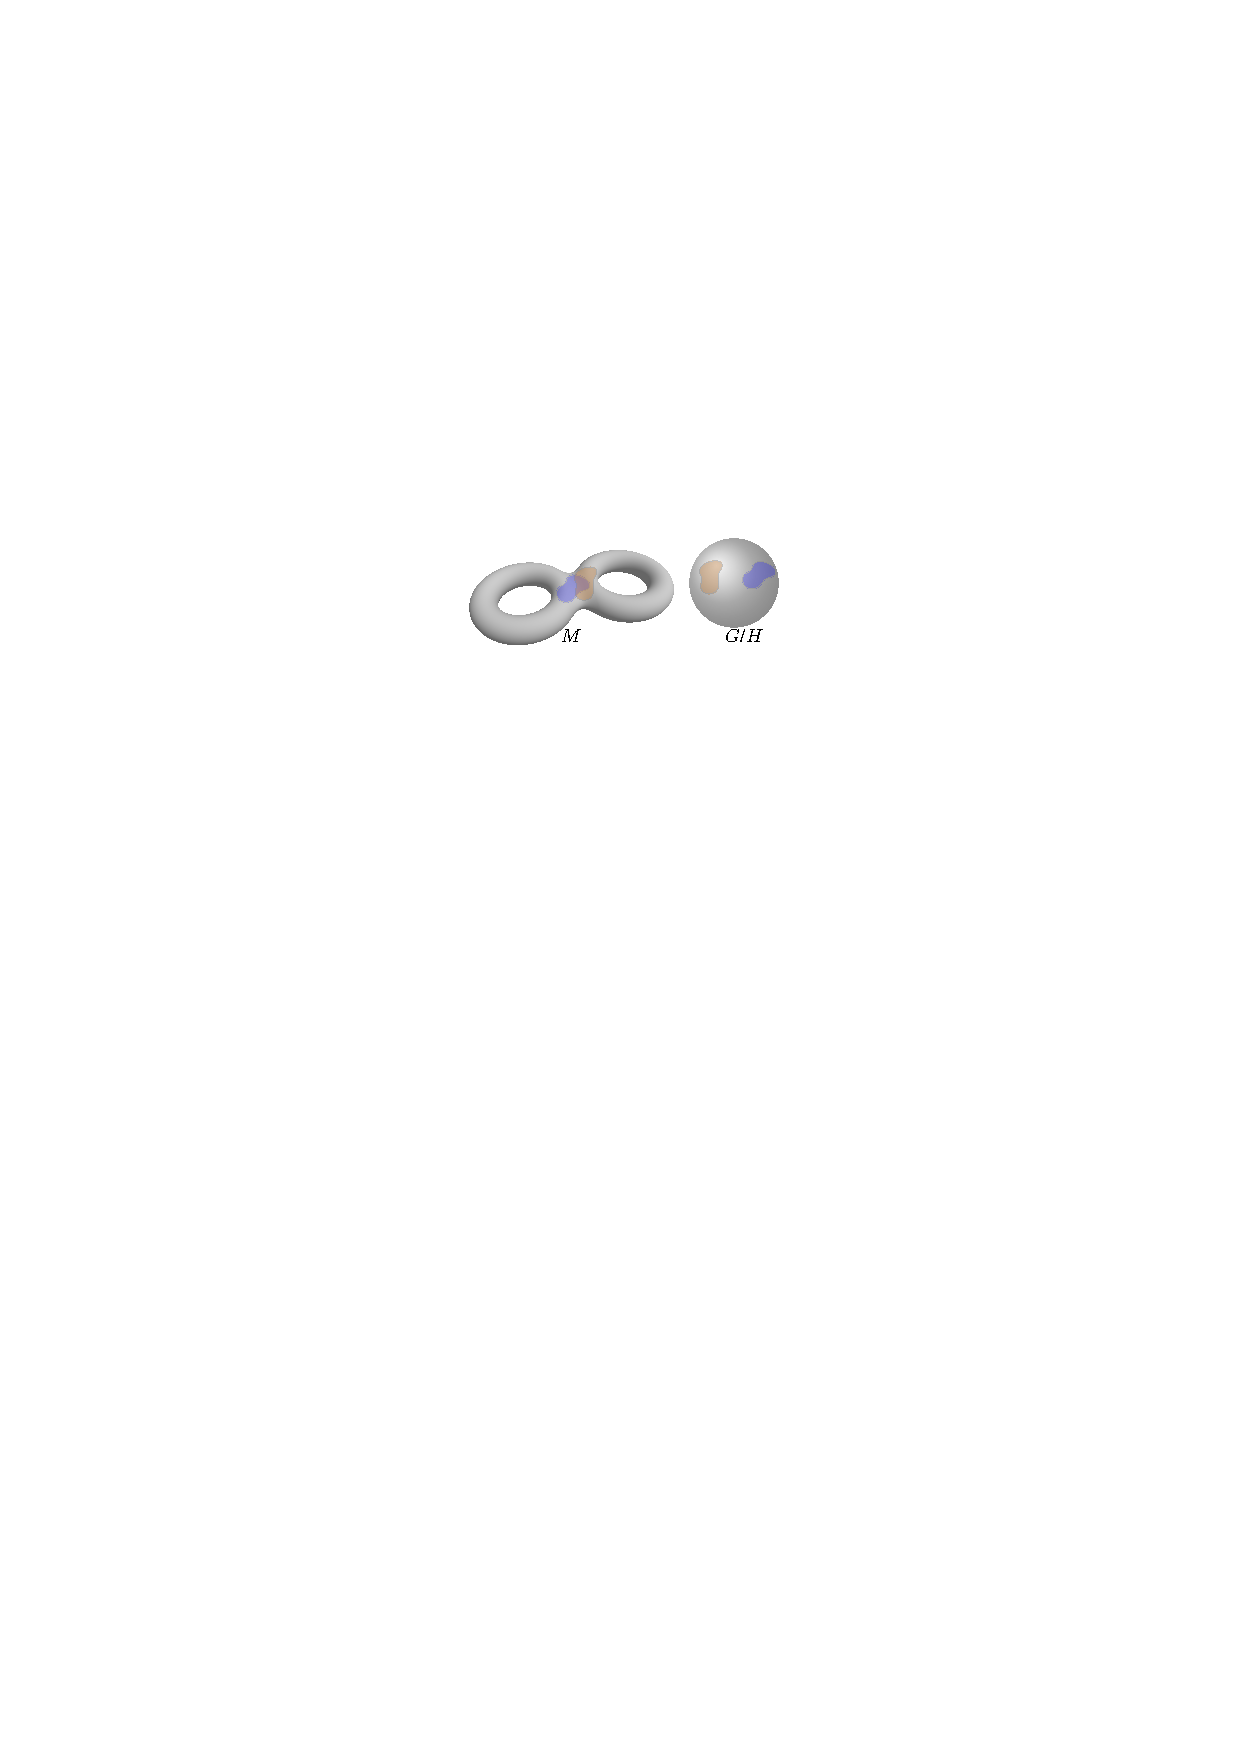
\includegraphics[scale=1.2]{figures/Klein.pdf}
    \caption{Effective locally Klein geometry.}
    \label{fig:klein}
\end{figure}

\begin{defn}[Effective $(G,H)$-structure]\label{def GH-structure}
    A locally homogeneous structure \emph{modeled on} an effective homogeneous space of type $(G,H)$ is a connected manifold $M$ with a \emph{$(G,H)$-atlas} $\{(U_\alpha,\varphi_\alpha)\}_\alpha$, where $\{U_\alpha\}$ is an open covering of $M$ and $\varphi_\alpha:U_\alpha\to \wh{U}_{\alpha}\subset G\slash H$ are diffeomorphisms such that for each non-empty intersection $U_{\alpha\beta}=U_\alpha\cap U_\beta$ there exists $g_{\beta\alpha}\in G$ such that 
    \[\varphi_{\beta}=\wh{L}_{g_{\beta\alpha}}\circ \varphi_\alpha\text{ on }U_{\alpha\beta}.\]
    A \emph{$(G,H)$-structure} on $M$ is a maximal $(G,H)$-atlas.
\end{defn}

We now show that this is indeed a special case of a locally Klein geometry, and the two definitions of effective locally Klein geometries are equivalent.

\begin{prop}
    An effective $(G,H)$-structure on $M$ induces a natural locally Klein geometry on $M$.
\end{prop}
\begin{proof}
    Since $(G,H)$ is effective, $\varphi_\alpha=\varphi_\beta$ on overlaps $U_{\alpha\beta}$. Consider the pullback principal $H$-bundles $P_\alpha=\varphi_\alpha^\ast G$. Since $\varphi_\alpha$'s agree on overlaps, $P_\alpha$'s stitch together into a principal $H$-bundle $P\to M$. The Maurer-Cartan form $\theta_G$ also pulls back to a $1$-form $\eta\in\Omega^1(P;\frakg)$ that satisfies all necessary properties.
\end{proof}


Finally, let us look at what kind of local differential forms can be defined on $M=\Gamma\bslash G\slash H$ using the Maurer-Cartan form. The following holds for Klein and locally Klein geometries.

\begin{prop}[{{\cite[Prop.~4.7.1]{Sharpe}}}]\label{prop 4.7.1 Sharpe}
    If $\chi:\pi^{-1}(U)\to U\times H$ is a local chart for the principal bundle $G\to G\slash H$ corresponding to the local section $ s:U\to G$. Then the local representative of the Maurer-Cartan form $\theta_G$ in this chart at point $(m,h)$ is $\Ad_h^{-1}\circ  s^\ast\theta_G +\pr_2^\ast\theta_H$, that is,
    \[(\chi^{-1})^\ast\theta_G(X_m,Y_h)=\Ad_h^{-1}\theta_G( s_\ast X_m)+\theta_H(Y_h),\quad X_m\in T_mU,Y_h\in T_h H.\]
\end{prop}
\begin{proof}
    We have $ s(m)=\chi^{-1}(m,e)$. Also let $i_h:U\to U\times H$ and $j_m:H\to U\times H$ be the inclusions of the slices $m\mapsto (m,h)$ and $h\mapsto (m,h)$, respectively. Then we have
    \[(\chi^{-1\ast}\theta_G)\circ i_{h\ast}=(\chi^{-1}\circ i_h)^\ast \theta_G=(R_h s)^\ast \theta_G= s^\ast R_h^\ast \theta_G= s^\ast(\Ad_h^{-1}\theta_G)=\Ad_h^{-1} s^\ast \theta_G,\]
    and on the other hand, 
    \[(\chi^{-1\ast}\theta_G)\circ j_{m\ast}=(\chi^{-1}\circ j_m)^\ast \theta_G=L_{ s(m)}^\ast\restr{\theta_G}{T_hH}=\restr{\theta_G}{T_hH}=\theta_H.\]
\end{proof}

Let $ s_\alpha:U_\alpha\to G$ be a local gauge, that is, a local section of the principal $H$-bundle $G\to G\slash H$ over an open set $U_\alpha\subset G\slash H$. Then $ s_\alpha$ pulls back the Maurer-Cartan form $\theta_G$ to a $\frakg$-valued $1$-form $\theta_\alpha$ on $U_\alpha$: \[\theta_\alpha\coloneqq  s_\alpha^\ast\theta_G.\] 
The Maurer-Cartan equation for $\theta_G$ then yields the Structure Equation for $\theta_\alpha$:
\[\dd\theta_\alpha+\frac 12[\theta_\alpha,\theta_\alpha]=0.\]
Note that $\theta_\alpha$ \emph{almost} determines $ s_\alpha$ since the Fundamental Theorem~\ref{thm 6.1 Sharpe fundamental local} says that $\theta_\alpha$ determines $ s_\alpha$ up to left multiplication by a fixed element of $G$. Then, for an effective Klein geometry, if $ s$ is a section, then $g s$ is a section iff $g=e$, so in this case $ s_\alpha$ is recovered uniquely.\footnote{If $g s$ is a section, then $u=\pi(g s(u))$ and hence $g\cdot u=u$ for all $u\in U$. Thus $f^{-1}gf\in H$ for all $f\in\pi^{-1}(U)\subset G$. Thus shows that $\{f\in G\mid f^{-1}gf\in H\}$ contains an open subset of $G$. But it is also an analytic subset of $G$, so it must be equal to $G$, at least for connected $G$. Thus $g\in \bigcap_{f\in G}fHf^{-1}$, and this latter is a normal subgroup of $G$ inside $H$ and is therefore trivial.} 
For this reason we may refer to $\theta_\alpha$ as an \emph{infinitesimal gauge}. We have the non-canonical isomorphism at every $m\in U_\alpha$
\[\underline{\theta}_\alpha:T_mU_\alpha\overset{\theta_\alpha}{\longrightarrow}\frakg\overset{\mod\frakh}{\longrightarrow} \frakg\slash\frakh.\]
The infinitesimal gauge $\theta_\alpha$ can be roughly interpreted as assigning to each tangent vector $X_m\in T_mM$ an infinitesimal ``motion'' $\theta_\alpha(X_m)\in \frakg$ of $M$ whose Killing vector field at $m$ coincides with $X_m$.

By differentiating the transformation rule $ s_\beta(m)= s_\alpha(m)h_{\alpha\beta}(m)$ (cf.\ (\ref{eq transf rule for sections})) we get
\[ s_\beta^{\ast}\theta_G=\Ad_{h_{\alpha\beta}}^{-1} s_\alpha^\ast\theta_G+h_{\alpha\beta}^\ast\theta_H,\]
that is
\[\theta_\beta=\Ad_{h_{\alpha\beta}}^{-1}\theta_\alpha+h_{\alpha\beta}^\ast\theta_H.\]
This transformation is called an \emph{infinitesimal change of gauge}, and the two infinitesimal gauges are called gauge equivalent.

Since in the effective case $\theta_\alpha$'s let us recover the local sections $s_\alpha$ uniquely, one can give an alternative definition of effective locally Klein geometries in terms of a collection of local $1$-forms on $M$ satisfying the Structure Equation and the above transformation rule. Unfortunately, this is not quite enough to recover the principal bundle because it needs to support \emph{complete} constant vector fields. Therefore, we shall delay this view of locally Klein geometry and return to it in our discussion of flat Cartan geometries. 

% \begin{defn}[Effective locally Klein geometry III]
%     An effective locally Klein geometry \emph{modeled on} an effective Klein geometry $(G,H)$ is a connected manifold $M$ with a collection $\{(U_\alpha,\theta_\alpha)\}_\alpha$, where $\{U_\alpha\}$  is an open covering of $M$ and each $\theta_\alpha\in \Omega^1(U_\alpha;\frakg)$ is a $\frakg$-valued local $1$-form that satisfies the Structure Equation 
%     \[\dd\theta_\alpha+\frac12 [\theta_\alpha,\theta_\alpha]=0,\]
%     and such that on every intersection $U_{\alpha\beta}$ there exists a smooth function $h_{\alpha\beta}:U_{\alpha\beta}\to G$ such that 
%     \[\theta_\beta=\Ad_{h_{\alpha\beta}}^{-1}\theta_\alpha+{h_{\alpha\beta}}^\ast\theta_H.\]
% \end{defn}




\begin{example}[Meteor tracking]
    Suppose we live in a small open set $U\subset M=G\slash H$ and a meteor flashes through $U$. We wish to describe its motion. We formalize the meteor as a point set $X$, and a \emph{configuration} of the meteor is a map $X_0:X\to M$. This is the origin for Cartan's idea of a ``moving frame''.\index{Moving frames}
    
    We assume the meteor is \emph{rigid} and \emph{sufficiently complicated}. By the term rigid in the given geometry, we mean that for any two of its positions, where it has the configurations $X_0$ and $X_1$ say, there is an element of $G$ carrying $X_0$ to $X_1$. By sufficiently complicated we mean that the subgroup of $G$ that fixes the body pointwise (its stabilizer) is the identity.  It follows that if $X(t)$ is the configuration of its points at time $t$, then there is a unique path $g(t)\in G$ such that $X(t)=g(t)X(0)$. One way to describe the motion would be to specify the path $g(t)$ itself. However, it is more useful, and closer to what is actually observed, to describe the motion differently. We first describe the motion of one of its points $q\in X(0)$, which we take to be $eH$, by a path $q(t)=g(t)H$ on $U$, and then describe the motion of the rest of the body as turning about this one point as it moves along. For this we will need the concept of a gauge.

    Let us assume that $U$ is small enough to admit a local section $s:U\to G$. Any two such sections $s,s'$ are related by a map $h:U\to H$ by $s'(u)=s(u)h(u)$. A ``choice of gauge'' is a choice of such a local section, and $h(u)$ is called a gauge transformation. A choice of gauge can be regarded as a choice of motions, varying smoothly with $u$, which maps the base point to $u$. The value of a gauge at any point may be called a \emph{frame} at that point and the gauge itself may be called a \emph{moving frame}. From this point of view the principal bundle $G\to G\slash H$ is a bundle of frames.

    Since both $s(q(t))$ and $g(t)$ lie over $q(t)$, they must differ by an element $k(t)\in H$. Thus, in the presence of a gauge, the motion can be described by giving $q(t)$ and $(k(t)$. The latter describes the way the meteor turns about the point $q(t)$. Crucially, there is no intrinsic geometric meaning attached to the choice of gauge $s$, or the function $k(t)$ alone. Together, however, they complete the description of the motion.
\end{example}


\begin{example}
    Recall the \emph{hyperbolic upper half-plane} $\bbC^+=\SL_2(\bbR)\slash \SO_2$ from Example~\ref{ex siegel upper half-space}. The Uniformization Theorem states that any closed (compact with no boundary) orientable surface $\Sigma_g$ of genus $g>1$ appears as the quotient $\Gamma\bslash \bbC^+$ for some choice of $\Gamma<\SL_2(\bbR)$. Let $\Gamma_g$ be such a subgroup. Then $\Sigma_g=\Gamma_g\bslash \bbC^+$ is a locally Klein geometry.
\end{example}

\begin{example}[Projective structure]\index{Projective structure}\label{ex projective structure}
    A \emph{Riemann surface}\index{Riemann surface}, also called a \emph{complex curve}, is a connected $1$-dimensional complex manifold $\Sigma$, i.e.\ its atlas consists of $\bbC$-valued maps with complex-analytic, or \emph{holomorphic}, transition maps (in the $1$-dimensional case holomorphic maps are also called \emph{conformal}, although the equivalence between these terms is nontrivial). Thus, the inverses of the transition maps are also complex-analytic, so that the transition maps are \emph{biholomorphic}.\index{Biholomorphism} Now, a \emph{projective structure} $\calP$ on $\Sigma$ is a $(\PSL_2(\bbC),\U_1)$-structure in the sense of Definition\ \ref{def GH-structure}. In particular, the chart maps are \emph{meromorphic} biholomorphisms, i.e.\ they take values in $\CP^1$ instead of just $\bbC$ (so they are allowed to have simple poles). The pair $(\Sigma,\calP)$ is called a \emph{complex projective surface}. Every Riemann surface admits many non-equivalent projective structures, but the Uniformization Theorem (stating that there is a unique, up to a \gls{flt}, biholomorphism between the universal cover of $\Sigma$ and one of three standard subsets of $\CP^1$) implies the existence of a \emph{canonical projective structure}.
\end{example}


\begin{example}[Monopole bundles]\label{ex monopole bundles}\index{Monopole!bundles}
    Consider the Hopf bundle $\bbS^3\to \bbS^2$ defined as a $\U_1$-principal bundle, or as a Klein geometry of type $(\SU_2,\U_1)$. Let $m\geq 1$ and $\Gamma=\bbZ_m\subset \U_1$ act on $\bbS^3$ by the restriction of the $\U_1$ action. The space $\Gamma\bslash \bbS^3$ is the loop space $L(m;1)$. We get the principal $\U_1$-bundle
    \[L(m;1)\to L(m;1)\slash \U_1=\bbS^2\]
    (since the induced action of $\U_1$ on $L(m;1)$ is trivial).
    Note that the structure groups here are abelian so right and left actions are indistinguishable.
    
    In the standard atlas consisting of two hemispheres (Example~\ref{ex hopf bundle atlas}), the transition function of this new bundle is $\tau_{-+}(z)=z^{-m}$, i.e.\ this is exactly the $\U_1$-bundle with Chern number $-m$ from Example~\ref{ex circle bundles over S2}. This proves that the lens space is simultaneously $\bbS^3\slash \bbZ_m$ and the gluing of two solid tori, thus solving Exercise~\ref{xca two definitions of lens spaces}. As principal $\U_1$-bundles, these bundles are known as \emph{monopole bundles}.

    We thus have the surjective vertical morphism of principal bundles $\vartheta:\bbS^3\to L(m;1)$ given by the quotient by the $\bbZ_m$-action and the group homomorphism $\lambda:\U_1\to \U_1$ given by the $m$-fold covering of the circle. Note that these bundles are also defined for $m$ negative as the duals (inverse transition functions), or via the inverse $\U_1$-action on $\bbS^3$.
\end{example}













\subsection{Homogeneous bundles}\label{sec: homogeneous bundles}


We now consider the tangent bundle of a Klein geometry. Since it is a locally trivial principal bundle, we have local diffeomorphisms of the form $T(\pi^{-1}(U))\cong T(U\times H)\to TU\times TH$. Local trivializations of $TU$ and $TH$ are given by the Maurer-Cartan forms $\theta_G$ and $\theta_H$, respectively, so the diagram
\[
\begin{tikzcd}
    T_g(gH)\arrow[r]\arrow[d,"\theta_H","\cong"'] & T_g G\arrow[r]\arrow[d,"\theta_G","\cong"'] & T_{m}(G\slash H)\arrow[d,dashed,"\chi_g","\cong"'] \\
    \frakh\arrow[r,hookrightarrow]&\frakg \arrow[r] & \frakg\slash \frakh
\end{tikzcd}
\]
is commutative with exact rows. Since $\frakh$  us only a subalgebra (not an ideal), the quotient $\frakg\slash\frakh$ is merely a vector space. The linear isomorphism $\chi_g$ is the unique map making the diagram commute.

We can identify the tangent space of $G\slash H$ at $m$ with $\frakg\slash\frakh$, but the identification $\chi_g$ depends on the choice of $g\in G$ over $m$. In fact, since $\pi\circ R_h=\pi$, the relation $R_h^\ast \theta_H=\Ad_h^{-1}\theta_H$ implies that $\chi_{gh}=\Ad_h^{-1}\circ \chi_g$. It follows that the identification of $T_m(G\slash H)$ with $\frakg\slash \frakh$ is determined only up to the adjoint action of $H$ on $\frakg\slash\frakh$. This accounts for the frequent occurrence of the adjoint action in the sequel. 

\begin{prop}[{{\cite[Prop.~4.5.1]{Sharpe}}}]\label{prop 4.5.1 Sharpe}
    $T(G\slash H)\cong G\times_H \frakg\slash\frakh$ as \glspl{vb} over $G\slash H$.
\end{prop}
\begin{proof}
    Define a map $\varphi:G\times \frakg\to T(G\slash H)$ by $\varphi(g, X)=(\pi(g),\pi_\ast \circ L_{g\ast}X)$, where $\pi:G\to G\slash H$ is the canonical projection. Clearly $\varphi$ is smooth, surjective, and fiberwise linear. Moreover, for $X\in T_eH$, $L_{g\ast}X\in T_g(gH)\in\ker\pi_\ast$. Thus, $\varphi(g, X)=(g,0)$. On the other hand,
    \begin{multline}
        \varphi(gh,\Ad_h^{-1}X)=(\pi(gh),\pi_\ast L_{gh\ast}\Ad_h^{-1}X)=(\pi(g),\pi_\ast(L_{gh\ast}L_{h\ast}^{-1} R_{h\ast}X))=\\
        =(\pi(g),L_{g\ast }\pi_\ast (R_{h\ast}X))=(\pi(g),L_{g\ast}(\pi R_h)_\ast X)
        =(\pi(g),L_{g\ast}(\pi_\ast X))=\varphi(g,X).
    \end{multline}
    Thus $\varphi$ induces a smooth quotient map $\wb\varphi:G\times_H \frakg\slash\frakh\to T(G\slash H)$. Moreover, this map is injective since $\varphi(g,X)=\varphi(g',X')$ implies $g'=gh$ for some $h\in H$ and $\pi_\ast L_{gh\ast}X'=\pi_\ast L_{g\ast}X$. The latter means that $\pi_\ast L_{h\ast}X'=\pi_\ast X$ and hence that $X'-\Ad_h^{-1}X\in\frakh$. Thus,
    \[[(g',X')]=[(gh,\Ad_h^{-1}X+\frakh)]=[(g,X+\frakh)]\in G\times_H\frakg\slash\frakh.\]
    Thus $\wb\varphi$ is a vertical \gls{vb} isomorphism.
\end{proof}


\begin{example}
    \begin{enumerate}
        \item Taking $\bbS^n=\SO_{n+1}\slash \SO_n$, we get the identification $T\bbS^n\cong \SO_{n+1}\times_{\SO_n}\bbR^n$, where $\bbR^n$ is the standard (defining) representation of $\SO_n$.
        \item Since the Grassmannian manifolds can be written as $\Gr_k(\bbK^n)\cong \calO_n\slash (\calO_{n-k}\times \calO_{k})$, by comparing transition functions it is easy to see that $T\Gr_k(\bbK^n)\cong \Hom(\gamma_k(\bbK^n),\gamma_k(\bbK^n)^\perp)$, where $\gamma_k(\bbK^n)$ is the tautological bundle over $\Gr_k(\bbK^n)$ and $\gamma_k(\bbK^n)^\perp$ is its orthogonal complement in $\Gr_k(\bbK^n)\times \bbK^n$.
    \end{enumerate}
\end{example}


Note that the basepoint $[e]=H\in G\slash H$ is preserved by the left action of $H$ via $\wh{L}_h$, $h\in H$, thus it generates an isotropy representation of $H$, which we specify in the following definition.

\begin{defn}[Isotropy representation]
    For a Klein geometry $(G,H)$, identify $T_{[e]}(G\slash H)$ with $\frakg\slash\frakh$ using the natural isomorphism constructed above. We call the induced representation $\underline{\Ad}:H\to \GL(\frakg\slash\frakh)$ given by $h\mapsto \wh{L}_{h\ast [e]}$, the isotropy representation of the Klein geometry.

    Since $\frakh<\frakg$ is invariant under $\Ad(H)$, the restriction of the adjoint representation to $H$, $\restr{\Ad}{H}:G\to \GL(\frakg)$, which descends to a map $H\to \GL(\frakg\slash h)$, which coincides with $\underline{\Ad}$.
\end{defn}

Since tangent bundles involve only first derivatives, we can make the following rough division of Klein geometries into two types according to whether $H$ is faithfully represented by this action.

\begin{defn}[First order Klein geometry]
    A Klein geometry $(G,H)$ is of first order if the isotropy representation $\underline{\Ad}:H\to \GL(\frakg\slash\frakh)$ is faithful. Otherwise, the geometry is said to have \emph{higher order}.
\end{defn}

\begin{rem}
    First order Klein geometries have a simple intuitive description in terms of $H$-structures. Since $H$ is faithfully represented on $\frakg\slash\frakh$, via the global trivialization of $TM$ constructed above, it traces out an $H$-orbit in the set of linear frames mapping $T_mM\to \frakg\slash\frakh$ for each $m\in M$. This was exactly our original definition of an $H$-structure on $TM$. Equivalently, this describes the principal bundle $G\to M$ as a reduction of the frame bundle $\Fr M$ to structure group $H$.
\end{rem}

The tangent bundle of a Klein geometry is an example of an important class of bundles that are equivariant with respect to the natural $G$-action $\wh L$ on the base $G\slash H$ in the following sense.


\begin{defn}[Homogeneous bundle]
    Let $G$ be a Lie group and $H\sub G$ a closed subgroup. A (left) homogeneous, or \emph{equivariant}, \gls{fb} of type $(G,H)$ is a \gls{fb} $E\overset{\pi}{\to}G\slash H$ over the homogeneous space of (left) cosets $G\slash H$ together with a (left) action $G\overset{\wt L}{\acts} E$ that lifts the natural (left) action $\wh L$ on $G\slash H$, i.e.\ which satisfies \[\pi\circ \wt{L}_g=\wh{L}_g\circ \pi,\text{ for all } g\in G.\] 

    In particular, a homogeneous \gls{vb} is a \gls{vb} which is also a homogeneous \gls{fb} such that the $G$-action is by \gls{vb} morphisms. Similarly, a homogeneous \gls{pfb} is a \gls{pfb} which is also a homogeneous \gls{fb} such that the $G$-action is by \gls{pfb} morphisms, i.e.\ by maps equivariant w.r.t.\ the (right) action of the structure group.

    A morphism of homogeneous bundles over $G\slash H$ is a vertical $G$-equivariant bundle morphism. The categories of homogeneous \glspl{fb} and \glspl{vb} are denoted $\FB_{(G,H)}$ and $\VB_{(G,H)}$, respectively. 
\end{defn}

\begin{example}
    The principal $H$-bundle $G\to G\slash H$ is obviously homogeneous because the left action $L$ is a lift of $\wh L$.
\end{example}

One common way of producing homogeneous bundles is by applying a natural bundle functor $F$ to $G\slash H$. Since by definition such a functor maps local diffeomorphisms to bundle morphisms, $F(\wh{L}_g)$ is a $G$-action as required in the definition of a homogeneous bundle. Thus, any natural bundle over a homogeneous space is homogeneous. As we will see below, the tangent bundle functor $T$ that we considered in the previous section is an example of this.

Let $E\to G\slash H$ be a homogeneous bundle. Consider the basepoint $[e]=eH\in G\slash H$ and the fiber $E_{[e]}$. The $G$-action on $E$ restricts to an $H$-action on $F$, thus we can build the associated bundle $G\times_H E_{[e]}\to G\slash H$. We now show that this bundle is isomorphic to $E$, thus characterizing all homogeneous bundles as bundles associated to principal bundles of the form $G\to G\slash H$.

\begin{thm}[{{\cite[Prop.~1.4.3]{Cap}}}]\label{prop 1.4.3 Cap}
    The mapping $E\to E_{[e]}$ (and restrictions of morphisms to the fiber) induces equivalences of categories $\FB(G,H)\simeq H\mathsf{-Man}$ and $\VB(G,H)\simeq H\mathsf{-FinVect}$, where $H\mathsf{-FinVect}$ is the category of finite-dimensional representations of $H$.
\end{thm}
\begin{proof}
    Consider the map $G\times E_{[e]}\to E$ given by $(g,f)\mapsto g\times f$, where we use the action of $G$ on $E$. Since the action $H\acts E_{[e]}$ is simply a restriction of this action, this map descends to a map $\varphi:G\times_H E_{[e]}\to E$ which is smooth since the projection $G\times E_{[e]}\to G\times_H E_{[e]}$ is a surjective submersion. Moreover, the definition $\varphi=g\cdot f$ implies that $\varphi$ covers the identity and is also right $G$-equivariant, so it is a morphism of homogeneous bundles.

    Now we build the inverse morphism. If $p\in E$, then by transitivity there exists a $g\in G$ such that $g\cdot \pi_E(p)=[e]$. Then $\pi_E(g\cdot p)=[e]$, so $g\cdot p\in E_{[e]}$, and we may consider $[(g^{-1},g\cdot p)]\in G\times_H E_{[e]}$. This is independent of the choice of $g$, since for another choice $g'\in G$ we must have $(g'g^{-1})\cdot p=p$, thus $g'g^{-1}\in H$, and thus
    \[[(g^{\prime-1},g'\cdot p)]=[(g^{\prime-1}g'g^{-1},gg^{\prime-1}g'\cdot p)]=[(g^{-1},g\cdot p)].\]
    Thus we get a well-defined map $\psi:E\to G\times_H E_{[e]}$. Choosing a local smooth section $s$ of $G\to G\slash H$ we can locally write $\psi(p)=[(s(\pi_e(p))^{-1},s(\pi_E(p))\cdot p)]$, which shows that $\psi$ is smooth. One immediately verifies that $\psi$ and $\varphi$ are mutually inverse bundle isomorphisms.

    To verify functoriality, if $\vartheta:E\to E'$ is a morphism of homogeneous bundles, then $\vartheta(E_{[e]})\subset E_{[e]}'$ and the restriction $\restr{\vartheta}{E_{[e]}}:E_{[e]}\to E_{[e]}'$ is $H$-equivariant. Equivariance of $\vartheta$ implies that for $g\in G$ and $f\in E_{[e]}$, we get $\vartheta(g\cdot f)=g\cdot \vartheta(f)$ which means that $\vartheta(\varphi([(g,f)]))=\varphi'([(g,\restr{\vartheta}{E_{[e]}}(f))])$, so we see that identifying $E$ and $E'$ with $G\times_H E_{[e]}$, respectively, $G\times_H E_{[e]}'$, the map $\vartheta$ is induced by $\id\times \restr{\vartheta}{E_{[e]}}$. Conversely, any $H$-equivariant map $F\to F'$ clearly induces a morphism of associated homogeneous bundles.

    Finally, note that for a homogeneous \gls{vb}, the above construction clearly produces an isomorphism $G\times_H E_{[e]}\to E$ of homogeneous \glspl{vb}, and homogeneous \glspl{vb} correspond to linear $H$-equivariant maps between their typical fibers.
\end{proof}

Thus an alternative definition of homogeneous bundles is simply as bundles associated to principal bundles of the form $G\to G\slash H$. Functoriality implies that these equivalences are compatible with various constructions such as fibered produces, Whitney sums, tensor products, etc. Conversely, for example, a decomposition of a tensor product of representations into a direct some of smaller representations induces a similar decomposition of corresponding Whitney products of homogeneous \glspl{vb}.

\begin{example}\label{ex 1.4.3 Cap}
    The  tangent  bundle $T(G\slash H)$ that we studied in Proposition~\ref{prop 4.5.1 Sharpe} is clearly homogeneous because the left action $\wh{L}_g$ on $G\slash H$ induces a lifted action $\wh{L}_{g\ast}$ on $T(G\slash H)$, and it corresponds to the $H$-representation on $\frakg\slash \frakh$ coming from the restriction to $H$ of the adjoint representation of $G$. The isomorphism with $G\times_H (\frakg\slash\frakh)$ established in that proposition is exactly the same as what we would obtain from Proposition~\ref{prop 1.4.3 Cap}. Namely, it maps $X\in T_{gH}(G\slash H)$ to $[(g^{-1},\omega(Y)+\frakh)]$, where $Y\in T_g G$ is some lift of $X$, i.e.\ $\pi_\ast Y=X$.

    By the naturality of the correspondence, the cotangent bundle $T^\ast(G\slash H)$ corresponds to the dual representation $(\frakg\slash\frakh)^\ast$. Note that the latter is just the annihilator of $\frakh$ in $\frakg^\ast$, so this is a subrepresentation of the restriction of the coadjoint representation of $G$ to $H$. Again, by naturality, the tensor bundle $T^k_l G\slash H$ corresponds to $\bbT^k_l(\frakg\slash\frakh)=(\frakg\slash\frakh)^{\otimes k}\otimes (\frakg\slash\frakh)^{\ast\otimes l}$.
\end{example}



Finally we provide a similar classification of principal homogeneous bundles.

\begin{prop}[{{\cite[Lem.~1.4.5]{Cap}}}]
    Let $(G,H)$ be a homogeneous space and $K$ a Lie group. Let $P\to G\slash H$ be a homogeneous principal $K$-bundle of type $(G,H)$. Then there is a smooth homomorphism $\lambda:H\to K$ such that $P\cong G\times_H K=G^{[\lambda]}$, where the action of $H$ on $K$ is $h\cdot k=\lambda(h)k$.

    The bundles corresponding to two homomorphisms $\lambda,\lambda':H\to K$ are (vertically) isomorphic  iff $\lambda$ and $\lambda'$ are conjugate, i.e.\ $\lambda'(h)=k\lambda(h)k^{-1}$ for some $k\in K$ and all $h\in H$.
\end{prop}
\begin{proof}
    Let $P_{[e]}$ be the fiber of $P$ over $[e]=eH\in G\slash H$. The left $G$-action on $P$ restricts to a left $H$-action on $P_{[e]}$, and $P\cong G\times_H P_{[e]}$ as homogeneous bundles. Fixing a point $p_0\in P_{[e]}$, the map $k\mapsto p_0\cdot g$ is a diffeomorphism $K\to P_{[e]}$, so it remains to describe the $H$-action in this picture.

    For $h\in H$, we have $h\cdot p_0\in P_{[e]}$, so there is a unique element $\lambda(h)\in K$ such that $h\cdot p_0=p_0\cdot \lambda(h)$. By smoothness of the two actions, the map $\lambda:H\to K$ defined this way is smooth, and $\lambda(e)=e$. Since $H$ acts by principal bundle maps, we see that $h\cdot (p_0\cdot k)=(h\cdot p_0)\cdot k=p_0\cdot \lambda(h)k$. From here, $\lambda$ is a homomorphism.

    Suppose that we are given an isomorphism $G\times_\lambda K\to G\times_{\lambda'}K$ of homogeneous \glspl{pfb}/ Then the restriction to the fibers over $[e]$ is a diffeomorphism $\phi:K\to K$ which commutes with the principal right $K$-action and is equivariant for the two left $H$-actions. By the first property, $\phi(k)=k_0k$, where $k_0=\phi(e)$. But then the second property reads as follows:
    \[k_0\lambda(h)k=\phi(\lambda(h)k)=\lambda'(h)\phi(k)=\lambda'(h)k_0k.\]
    In particular, $\lambda'(h)=k_0\lambda(h)k_0^{-1}$. Conversely, if $\lambda$ and $\lambda'$ are conjugate, right multiplication by $k_0$ induces a diffeomorphism with the two required equivariance properties. From Proposition~\ref{prop 1.4.3 Cap} we conclude that this gives rise to an isomorphism of homogeneous principal bundles. 
\end{proof}





\subsection{Kernels and jets}


Since we will in the future describe the group $G$ of a Klein geometry $(G,H)$ as defining a certain geometric structure on the manifold $G\slash H$, it is important to better understand the induced $G$-action on $G\slash H$, which is not necessarily faithful. In particular, the kernel $K$ acts trivially on $G\slash H$ and hence on the model tangent space $\frakg\slash\frakh$. However, the kernel of the isotropy representation $\underline{\Ad}:\frakh\to \GL(\frakg\slash\frakh)$ does not necessarily coincide with $K$ (it might be larger). In this section we examine how one could nevertheless compute $K$ using only infinitesimal information.

Let $G$ be a Lie group with Lie algebra $\frakg$. To each linear subspace $\frakl<\frakg$ and closed subgroup $H\sub G$, associate the closed subgroup $K_\frakl\sub H\sub G$ defined as follows:
\[K_\frakl\coloneqq \left\{h\in H\mid \forall A\in\frakg\;\; \Ad_h A-A\in \frakl\right\},\]
i.e.\ $\frakl$ is $K_\frakl$-invariant and the induced action of $\Ad(K_\frakl)$ on $\frakg\slash\frakl$ is also trivial.

\begin{lem}
    If $\frakl<\frakh$ is an $\Ad(H)$-invariant linear subspace then $K_\frakl\sub H$ is a closed normal subgroup.
\end{lem}
\begin{proof}
    For any $h\in H$ and $a\in H_\frakl$, the operator
    \[\Ad_{hah^{-1}}-\id_\frakg=\Ad_h\Ad_a\Ad_h^{-1}-\id_\frakg=\Ad_h(\Ad_a-\id_\frakg)\Ad_h^{-1}\]
    maps $\frakg$ to $\Ad_h (\frakl)=\frakl$ by definition of $K_\frakl$. Thus, $hah^{-1}\in K_\frakl$ and $K_\frakl$ is normal.
\end{proof}

Now let 
\[K_1\coloneqq K_{\frakh},\quad K_{i+1}\coloneqq K_{\frakk_i},\quad i\geq 1.\]
By induction, since $K_i\sub H$ is normal, $\frakk_i<\frakh$ is an ideal, and $K_{i+1}\sub H$ is also a closed normal subgroup (of $H$).

\begin{lem}
    If $(G,H)$ is a Klein geometry with kernel $K$ and $K_i\sub H$ is the sequence of normal subgroups of $H$ defined above, then 
    \[K=\bigcap_{i=1}^\infty K_i.\]
\end{lem}
\begin{proof}
    Let $M=G\slash H$. Every element $h\in K$ by definition acts trivially on $M$, hence preserves $\frakh$ and acts trivially on $\frakg\slash\frakh=T_{[e]}(G\slash H)$, so lies in $K_1=K_{\frakh}$. Thus, $M_1\coloneqq G\slash K_1$ is identified with a $G$-invariant set of linear isomorphisms $T_m M\to \frakg\slash\frakh$, $m\in M$. Therefore, $K$ acts trivially on $M_1$ as well. By induction, $K\subset \bigcap_i K_i$.

    % Denote by $G_0$ the identity component of $G$. Let $G'<G$ be the subgroup generated by $G_0\cup H$. Let $G''$ be the union of all connected components of $G$ of the coset form $hG_0$, $h\in H$. First, we show that $G''=G'$. Clearly $H\cup G_0\subset G''$ and each component $hG_0$ lies in $G'$, so $G''\subset G'$. On the other hand, for $h,h'\in H$, $hG_0g'G_0=hh'G_0$ because $G_0$ is a normal subgroup of $G$, therefore $G''$ is a subgroup of $G$. Finally, since $G''$ contains both $G_0$ and $H$, it contains the group generated by them, which is $G'$. Hence, $G'=G''$.

    Suppose that $N$ is a normal subgroup of $G$ that lies inside $H$. Then for $g\in G$ and $n\in N$,
    \[n(gH)=(ng)H=gNH=gH,\]
    so $N$ stabilizes every point of $M$, and thus $N<K$. Let $K'\coloneqq \bigcap_i K_i$. This is a closed subgroup by virtue of being the intersection of closed subgroups. Its Lie algebra $\frakk'$ is the smallest of the nested $\frakk_i$. For any $A\in\frakg$ and $k\in K'$, 
    \[\Ad_k A-A\in\frakk'.\]
    Thus, $\Ad_k$ acts trivially on $\frakg\slash\frakk'$. We can exponentiate in $G\slash K'$ to conclude that $\Adg_k$ acts trivially on the identity component $(G\slash K')_0$. In other words, $K'$ commutes with $(G\slash K')_0$, which means that $K'$ is normal in $G_0$ and in $H$, and thus normal in $G$ (which is generated by $G_0$ and $H$ since $G\slash H$ is connected by definition of Klein geometry). Thus, $K'\subset K$.
\end{proof}

As an immediate corollary, we find the following infinitesimal description of the kernel.

\begin{thm}[{{\cite[Thm.~4.4.1]{Sharpe}}}]\label{thm 4.1 Sharpe}
    Let $(G,H)$ be a Klein geometry with kernel $K$ and $\frakk=\Lief K$. Then 
    \[K=\{h\in H\mid \Ad_h X-X\in\frakk \text{ for all }X\in\frakg\}.\]
\end{thm}

As a special case, in effective Klein geometries there are no proper subgroups of $H$ whose lie algebra is $\Ad(H)$-invariant.

\begin{cor}[Fundamental property of effective Klein geometries{{\cite[Cor.~4.4.2]{Sharpe}}}]\label{Cor 4.2 Sharpe}
    If $(G,H)$ is an effective Klein geometry, $N$ is a subgroup of $H$, and $\frakn=\Lief N$, then
    \[N=\{h\in H\mid \Ad_h X-X\in\frakn \text{ for all }X\in\frakg\}\Rightarrow N=\{e\}.\]
\end{cor}

\begin{example}[Real projective space]\label{ex real projective Klein model}
    Consider the projective space $\RP^n$ as a homogeneous space of type $(G=\SL_{n+1}(\bbR),H)$ with $H$ the stabilizer of the basepoint $[e]=[\bf{e}_{n+1}]$, i.e.\ the set of unimodular matrices preserving $\bf{e}_{n+1}$ up to a scale. $H$ consists of matrices of the form 
    \[ \begin{pmatrix}
        a & \bf{0}_n \\
        \bf{x}^T & (\det a)^{-1} 
    \end{pmatrix},\quad a\in \GL_n(\bbR),\bf{x}\in\bbR^n.\]
    $H$ acts on $\frakg=\fraksl_{n+1}(\bbR)$ via conjugation. The tangent space $T_{[e]}(\RP^n)=\frakg\slash\frakp$ then consists of elements of the form 
    $\left(\begin{smallmatrix}
        \ast & \bf{y} \\
        \ast & \ast
    \end{smallmatrix}\right)$, where $\ast$ stands for the entirety of the subspaces of $\frakh$ spanned by the corresponding components of the matrix. The $\Ad(H)$-action on this space reads 
    is acted on via 
    \[\begin{pmatrix}
        a & \bf{0}_n\\
        \bf{x}^T & (\det a)^{-1}
    \end{pmatrix}
    \begin{pmatrix}
        \ast & \bf{y} \\
        \ast & \ast 
    \end{pmatrix}
    \begin{pmatrix}
        a & \bf{0}_n\\
        \bf{x}^T & (\det a)^{-1}
    \end{pmatrix}^{-1}=
    \begin{pmatrix}
        \ast & (\det a) a\bf{y} \\
        \ast & \ast
    \end{pmatrix}.
    \]
    Thus, the elements of $H$ that act trivially on $T_{[e]}(\RP^n)$ are precisely the subgroup $K_1\subset H$ of matrices with $a\bf{y} (\det a)=\bf{y}$ for all $\bf{y}\in\bbR^n$, i.e.\ 
    \[K_1=\left\{ 
        \begin{pmatrix}
            \lambda \rmI_n & \bf{0}_n \\
            \bf{x}^T & \lambda
        \end{pmatrix} \middle| \bf{x}\in\bbR^n,\lambda\in\bbR, \lambda^{n+1}=1
    \right\}, \quad \frakk_1=\left\{ 
        \begin{pmatrix}
            \mathrm{0}_{n,n} & \bf{x} \\
            \bf{0}_n^T & 0
        \end{pmatrix} \middle| \bf{x}\in\bbR^n\right\}.\]
    This subgroup $K_1<G$ is precisely the subgroup preserving both $[e]=[\bf{e}_{n+1}]\in\RP^n$ and the standard basis for $T_{[e]}\RP^n$, so $G\slash K_1\to \RP^n$ is the frame bundle of $\RP^n$, i.e.\ the set of pairs $(m,u)$ of point $m\in \RP^n$ and linear isomorphism $u:T_m\RP^n\to \bbR^n$.  To act trivially on $\RP^n$, an element of $G$ must lie in $K_1$, but it must also act trivially on the frame bundle of $\RP^n$, i.e.\ on $G\slash K_1$. By the same reasoning, it must act trivially on $T_{u_0}(G\slash K_1)$, where $u_0$ is the standard basis of $\bbR^n$ viewed as a frame on $\RP^n$. But $T_{u_0}(G\slash K_1)=\frakg\slash\frakk_1$, and we compute that $K_1$ acts on $\frakg\slash\frakk_1$ by 
    \[\begin{pmatrix}
        \lambda\rmI_n & \bf{0}_n\\
        \bf{b}^T & \lambda
    \end{pmatrix}
    \begin{pmatrix}
        A & \bf{y} \\
        \ast& d
    \end{pmatrix}
    \begin{pmatrix}
        \lambda\rmI_n & \bf{0}_n\\
        \bf{b}^T & \lambda
    \end{pmatrix}^{-1}=
    \begin{pmatrix}
        A-\lambda^{-1}\bf{y}\bf{b}^T& \bf{y}\\
        \ast  & d+\lambda^{-1}\bf{b}^T\bf{y}
    \end{pmatrix}.
    \]
    Now, $K_2$ is the set of elements of $K_1$ that act trivially, i.e.\ $0=\lambda^{-1}\bf{y}\bf{b}^T=\lambda^{-1}\bf{b}^T\bf{y}$ for all vectors $\bf{y}$, hence $\bf{b}=0$. Thus, $K_2$ is 
    \[K_2=\left\{ 
        \begin{pmatrix}
            \lambda \rmI_n & 0 \\
            0 & \lambda
        \end{pmatrix} \middle| \lambda\in\bbR, \lambda^{n+1}=1
    \right\}=\rmZ(\SL_{n+1}(\bbR)).\]
    This is clearly the kernel of this Klein geometry, as these are precisely the elements of $G$ that act trivially on $\RP^n$. As a consequence, the projective model $\RP^n\cong \PSL_{n+1}(\bbR)\slash (H\slash K)$ is effective.
\end{example}


Next, recall that the $r$-jet of a smooth map can be identified, given a particular coordinate chart, with the Taylor series of that map up to and including $r$-th order derivatives. We now show that $K_r$ consists of exactly those elements of $G$ which induce diffeomorphisms of $G\slash H$ with trivial derivatives up to order $r$ (by trivial we mean they coincide with the derivatives of the identity map).

\begin{lem}
    The subgroup $K_r\sub G$ is precisely the set of elements $g\in G$
    such that the $r$-th jet at $[e]$ of the induced action $\wh{L}_g$ on $M=G\slash H$ is the same as that of the identity map:
    \[K_r=\left\{g\in G: j^k_{[e]}\wh{L}_g=j^k_{[e]}\id_{M}\right\}.\]
\end{lem}
\begin{proof}
    For $r=1$, $K_1=K_{\frakh}$ is the set of elements $h\in H$ such that $\underline{\Ad}_h$ is trivial. But, as established above, $\underline{\Ad}$ is exactly the isotropy representation of the action $\wh{L}$, i.e.\ $\underline{\Ad}_h$ being trivial is equivalent to the first derivative of $\wh{L}_h$ at $[e]$ being the identity.

    Now we prove for $r>1$ by induction. Assume that the statement is known for all $i\leq r-1$. To each $g\in G$ we associate the $r$-th order jet $j^r_{[e]}\wh{L}_g$ (its target is $gH\in M$). This defines a smooth map into the $r$-th jet space (and in particular invertible $r$-jets):
    \[\Phi_r\coloneqq j_{[e]}^r\circ \wh{L}_{\smbullet}: G\to J^r_{[e]}(M,M)^\times.\]
    By hypothesis, $K_{r-1}$ is exactly the elements of $G$ whose $r$-jets are trivial:
    \[K_{r-1}=\Phi_{r-1}^{-1}\left(e_r\right), \quad \text{ where }e_r\coloneqq j^r_{[e]}\id_M.\]
    Thus, $\Phi_{r-1}$ descends to an \emph{injective immersion} of the qutient manifold
    \[\varphi_{r-1}:G\slash K_{r-1}\hookrightarrow J^{r-1}_{[e]}(M,M)^\times.\]
    Therefore, we can identify $G\slash K_{r-1}$ with the submanifold $\varphi_{r-1}(G\slash K_{r-1})< J^{r-1}_{[e]}(M,M)^\times$, and replace the action $\wh{L}_k$, $k\in K_{r-1}$ on $G\slash K_{r-1}$ with the action of $j^{r-1}_{[e]}\wh{L}_k$ on $J^{r-1}_{[e]}(M,M)^\times$ by pre-composition of jets. This is well-defined because $\wh{L}_k$ preserves the basepoint of $G\slash K_{r-1}$.
    
    By definition, $K_r$ is the subgroup of $K_{r-1}$ acting trivially on the tangent space of $G\slash K_{r-1}$ at the basepoint, i.e.\ the kernel of the isotropy representation of the Klein geometry $(G,K_{r-1})$. Thus, via the above identification with a submanifold of $J^{r-1}_{[e]}(M,M)^\times$, the subgroup $K_r$ can be identified with those elements of $K_{r-1}$ whose $1$-jets of the $(r-1)$-jets vanish. But this is the same as the vanishing of the $r$-jets: 
    \[K_r=\left\{k\in K_{r-1}: j^1_{[e]}\circ j^{r-1}_{[e]}\circ\wh{L}_k=e_r\right\}=\left\{g\in G: j^r_{[e]}\circ \wh{L}_g=e_r\right\}.\]
    Indeed, since $\varphi_{r-1}$ is an immersion, the triviality of the derivative of its composition with $\wh{L}_k$ is equivalent to the triviality of the derivative of $\wh{L}_k$ itself. This concludes the induction step.
\end{proof}



\begin{example}[\ref{ex real projective Klein model} continued]
    Consider the projective space $\RP^n$ viewed as a Klein geometry $(G,H)$ with $G=\PGL_{n+1}$. As we saw, $G\slash K_1$ is the frame bundle of $\RP^n$, i.e.\ all of $J^1_{[e]}(\RP^n,\RP^n)^\times$. Thus, any linear isomorphism of tangent spaces of $\RP^n$ arises as the first derivative of a projective transformation. Then $K_2$ is trivial, and $G\slash K_2=G=\PGL_{n+1}\subset J^2_{[e]}(\RP^n,\RP^n)^\times$ is the set of $2$-jets of projective transformations: a projective transformation is determined by its $2$-jet. Moreover, the set of $2$-jets with a given $1$-jet is $K_1\slash K_2=K_1$, the group of projective transformations of the form 
    \[\begin{pmatrix}
        \rmI_n & \bf{0}_n\\
        \bf{x}^T & 1
    \end{pmatrix},\quad \bf{x}\in\bbR^n,\]
    modulo multiplication by $(n+1)$-roots of unity.  So the space of $2$-jets of projective transformations with a given $1$-jet has dimension $n$.
\end{example}

\begin{example}[Complex projective space]
    Similarly, $\CP^n\cong \SL_{n+1}(\bbC)\slash H$, where $H$ is the stabilizer of $[\bf{e}_{n+1}]$. We also note that $\PSL_{n+1}(\bbC)\cong \PGL_{n+1}(\bbC)$ (cf.\ Exercise~\ref{xca psl=pgl}), and everything we found in Example~\ref{ex real projective Klein model} carries over to the complex case with the substitution $\bbR \to \bbC$. We find that the kernel is 
    \[K=K_2=\rmZ(\SL_{n+1}(\bbC))=\{\lambda \rmI_{n+1}\mid \lambda\in\bbC ,\lambda^n=1\}.\]
    As a consequence, the projective model $(\PSL_{n+1}(\bbC),H\slash K)=(\PGL_{n+1}(\bbC),H\slash K)$ is effective. 

    The most important example of course is the Riemann sphere $\CP^1=\PGL_2(\bbC)\slash (H\slash K)$, where $\PGL_2(\bbC)$ is the M\"obius group 
\end{example}







\subsection{Frobenius reciprocity}\label{sec: Frobenius reciprocity}

Consider the set $\Gamma^\infty(E)$ of sections of a homogeneous vector bundle $E\to G\slash H$. There is a natural left $G$-action on $\Gamma^\infty(E)$ defined by
\[g\cdot s\coloneqq \wt{L}_g\circ s\circ\wh{L}^{-1}_g,\]
where $\wt L$ and $\wh L$ are the actions on $E$ and $G\slash H$, respectively. Note that this particular combination of the two actions is required so that sections get mapped to sections, i.e.\ so that the action preserves the point in the base.

\begin{defn}[Induced representation]\index{Induced representation}
    Let $(G,H)$ be a homogeneous space, $G\acts V$ a finite-dimensional linear representation $G$, and $E=G\times_H V$ be the corresponding homogeneous \gls{vb}. The representation of $G$ on $\Gamma^\infty(E)$ defined above is called the \emph{induced representation} of $G$, denoted $\Ind^G_H(V)$. The association functor for bundles makes this a functor of $V$.

    In addition, we denote by $\Res^G_H(V)$ the representation of $H$ on $G$ obtained by restriction of the representation of $G$. This is also obviously functorial in $V$.
\end{defn}

The correspondence between sections of an associated bundle and equivariant functions on the principal bundle (Proposition~\ref{prop 1.2.6 RS2}) gives rise to another interpretation of the induced action of $G$ on sections. This picture is (in the case of homogeneous \glspl{vb}) frequently used in representation theory. Namely, via the isomorphism $E\cong G\times_H E_{[e]}$ from Proposition~\ref{prop 1.4.3 Cap}, we can identify $\Gamma^\infty(E)$ with $\Gamma\left(G\times_H E_{[e]}\right)$, which in turn by Proposition~\ref{prop 1.2.6 RS2} is in bijective correspondence with the set $\Hom_H(G,E_{[e]})$. Explicitly, the correspondence between a section $s$ and a function $\varphi$ is characterized by $s(gH)=[(g,\varphi(g))]=g\cdot \varphi(g)$ or by $\varphi(g)=g^{-1}\cdot s(gH)$. In the case of a homogeneous vector bundle, this bijection is clearly a linear isomorphism.

To get the action of $G$ on $\Gamma^\infty(E)$ in the picture of equivariant functions, we only have to notice that by definition $(g\cdot  s)(g'H)=g\cdot  s(g^{-1}g'H)$. Consequently, the map $g\cdot f:G\to E_{[e]}$ corresponding to $g\cdot s\in \Gamma^\infty(E)$ is given by none other than the natural action by pullbacks $L_g^\ast$:
\[(g\cdot \varphi)(g')=g^{\prime-1}\cdot(g\cdot s(g^{-1}g'H))=(g^{-1}g')^{-1}\cdot s(g^{-1}g'H)=\varphi(g^{-1}g').\]

The next fundamental result shows that in certain situations one can reduce questions about the infinite-dimensional space $\Gamma^\infty(E)$ to questions about the finite-dimensional manifold $E_{[e]}$. In particular, determining $G$-invariant sections of a homogeneous bundle always reduces to a finite-dimensional problem.

\begin{thm}[Geometric Frobenius reciprocity {{\cite[Thm.~1.4.4]{Cap}}}]\label{thm 1.4.4 Cap}
    Let $E\to G\slash H$ be a homogeneous bundle with standard fiber $E_{[e]}$ (viewed as an $H$-space), and let $X$ be a smooth manifold endowed with a smooth left $G$-action. Then the evaluation at $[e]$ induces a natural bijection between the set of $G$-equivariant maps $X\to \Gamma^\infty(E)$ and the set of $H$-equivariant maps $X\to E_{[e]}$. In particular, there is a natural bijection between the set $\Gamma^\infty(E)^G$ of $G$-invariant sections of $E$ and the set $(E_{[e]})^H$ of $H$-invariant elements of the typical fiber.

    If $E$ is the homogeneous \gls{vb} induced by an $H$-representation $W$, and $V$ is a representation of $G$, then the bijections above are linear and respect the subspaces of linear equivariant maps, so that there is a natural linear isomorphism
    \[\Hom_G\left(V,\Ind^G_H(W)\right)\cong \Hom_H\left(\Res^G_H(V),W\right),\]
    i.e.\ $\Res^G_H$ and $\Ind^G_H$ are adjoint functors.
\end{thm}
\begin{proof}
    Suppose are given a map $X\to\Gamma^\infty(E)$ writen as $x\mapsto  s_x$. This map is $G$-equivariant iff $ s_{g\cdot x}(g'H)=g\cdot s_x(g^{-1}h'H)$. In particular, if we consider the map $X\to E_{[e]}$ defined by $x\mapsto  s_x([e])$, then for $h\in H$, we get $ s_{h\cdot x}([e])=h\cdot  s_x(h^{-1}\cdot[e])=h\cdot s_x([e])$, so this is $H$-equivariant. 
    
    Conversely, if $\varphi:X\to E_{[e]}$ is $H$-equivariant, then for $x\in X$ we define $ s_x:G\slash H\to E$ by $ s_x(gH)=g\cdot \varphi(g^{-1}\cdot x)$. This is well defined since $\varphi(h^{-1}g^{-1}\cdot x)=h^{-1}\cdot \varphi(g^{-1}\cdot x)$, and thus $gh\cdot \varphi(h^{-1}g^{-1}\cdot x)=g\cdot \varphi(g^{-1}\cdot x)$. Moreover, $ s_x([e])=\varphi(x)$ and 
    \[ s_{g\cdot x}(g'H)=g'\cdot \varphi(g^{\prime-1}g\cdot x)=g\cdot g^{-1}g'\cdot \varphi(g^{\prime-1}g\cdot x)=g\cdot s_x(g^{-1}g'H),\]
    so $x\mapsto  s_x$ is $G$-equivariant. Since for any $G$-equivariant map $x\mapsto  s_x$ we must have $ s_x(gH)=g\cdot g^{-1}\cdot  s_x(g^{-1}gH)=g\cdot  s_{g\cdot x}([e])$, the two constructions are inverse bijections between the set of $G$-equivariant maps $X\to \Gamma^\infty(E)$ and the set of $H$-equivariant maps $X\to E_{[e]}$.

    Taking $X=\{*\}$ a single point with the trivial $G$-action, a $G$-equivariant map $X\to \Gamma^\infty(E)$ is just a $G$-invariant section $g\cdot  s_*= s_*$, and a $H$-equivariant map $X\to E_{[e]}$ is an $H$-invariant element in $E_{[e]}$. Thus we get a bijection $\Gamma^\infty(E)^G\to (E_{[e]})^H$.

    Finally, if $E$ is a natural \gls{vb} induced by an $H$-representation $W$ and $X$ is a $G$-representation $V$, then $\Lin(V,\Gamma^\infty(E))$ and $\Lin(V,E_{[e]})$ are vector spaces under the pointwise operations, and the evaluation at $[e]$ induces a linear map $\Lin(V,\Gamma^\infty(E))\to \Lin(V,E_{[e]})$. If we start from a linear map $\varphi:V\to E_{[e]}$, the construction above produces $ s_v(gH)=g\cdot \varphi(g^{-1}\cdot v)$. Since $\varphi$ is linear and $G$ acts by linear maps, this is linear in $v$.
\end{proof}

\begin{example}[Spherical harmonics]
    Looking ahead, we can take $H$ to be a maximal torus subgroup $T\sub G$. Since $T$ is abelian, its irreducible representations (irreps) are one-dimensional and are called \emph{weights}, labeled by $\lambda$. The associated homogeneous line bundles over $G\slash T$ are denoted $L_\lambda$. Further if $V_\gamma$ is an irrep of $G$ (labeled by a highest weight $\gamma$, irrelevant to this statement), then by Schur's Lemma the dimension of the space $\Hom_G(V_k,\Gamma^\infty(L_n))$ is simply counting the multiplicity of $V_k$ in the decomposition of $\Gamma^\infty(L_n)$ into irreps. Therefore the Frobenius reciprocity in the language of representation theory states that the multiplicity of a $G$-irrep $V_\gamma$ in the decomposition of $\Gamma^\infty(L_\lambda)$ is equal to the multiplicity of the weight $\lambda$ in $V_\gamma$. If $G$ is compact, then for any given weight $\lambda$, the induced representation $\Gamma^\infty(L_\lambda)$ will decompose into an infinity of irreducibles (because each is finite-dimensional for compact $G$), namely all those that contain the weight $\lambda$.

    Consider $G=\SU_2$ and $T=\U_1$ the subgroup fixing a vector. Then $G\slash T\cong \bbS^2$. Since $T$ is abelian, all of its representations decompose into sums of one-dimensional (hence irreducible) ones, and the one-dimensional representations are labeled by an integer $n\in\bbZ$ (namely the representation is given by multiplication by $z^n$, where $z\in\U_1\subset \bbC$). Meanwhile the irreducible representations $V_k$ of $\SU_2$ are known to be labeled by non-negative integers $k$, where $k$ is the largest integer that occurs when you restrict $V_k$ to be a $\U_1$ representation. Frobenius reciprocity implies
    \[\dim\Hom_{\SU_2}(V_k,\Gamma^\infty(L_n))=\dim \Hom_{\U_1}(V_k,n)\]
    where $L_n$ is the complex line bundle over $\bbS^2$ corresponding to $n$. The right hand side is the multiplicity of the weight $n$ in $V_k$ (that is, the multiplicity of $n$ in the restriction of the representation on $V_k$ to $T$). Since we know what the weights of $V_k$ are ($-k,-k+2,\ldots,k-2,k$, all with multiplicity one), we can see that the decomposition of $\Gamma^\infty(L_n)$ into irreducibles will include all $V_k$ where $k$ is the same parity as $n$ and $k\geq n$.

    In the case $n=0$, $L_0$ is the trivial $\bbC$-bundle and $\Gamma^\infty(E_0)\cong C^\infty(\bbS^2,\bbC)$ is just the space of complex-valued functions on $\bbS^2$. Only $V_k$ with even $k$ include the weight $0$, therefore $C^\infty(\bbS^2,\bbC)$ decomposes into a sum of such irreps. To compute the multiplicity of each of them, we use Frobenius reciprocity. As stated above, the multiplicity of $n=0$ in $V_{2l}$ is $1$. For analytic reasons that will be clarified in the Peter-Weyl theorem, the direct sum of all $V_{2l}$'s, once endowed with a proper topology, is not exactly $C^\infty(\bbS^2)$, but rather the Hilbert space $L^2(\bbS^2)$ of square integrable functions:
    \[L^2(\bbS^2,\bbC)\cong \bigoplus_{l=0}^\infty V_{2l}.\]
    This holds both over reals and complexes. The space $V_{2l}$ is $(2l+1)$-dimensional and a standard basis is given by the spherical harmonics $Y^l_m(\theta,\varphi)$. If we replace $\SU_2$ by $\SO_3$, the only difference is that $V_k$ with odd $k$ disappear from the list of irreps, so the final result for $n=0$ is the same. This is the beginning of the subject of \emph{harmonic analysis} (and in particular Fourier transforms) on Lie groups.
\end{example}








The geometric version of Frobenius reciprocity immediately allows us to reduce questions about the existence of invariant Riemannian metrics and other invariant tensor fiels to problems of finite-dimensional representation theory: if $M=G\slash H$ is a homogeneous space, then from Proposition~\ref{prop 1.4.3 Cap} we know that the tensor bundle $\bbT^k_lM$ is associated to $G\to M$ with respect to the representation $\bbT^k_l(\frakg\slash \frakh)$. By Frobenius reciprocity, $G$-invariant sections of this bundle are in bijective correspondence with $H$-invariant elements in the representation. Since invariant elemnets are the same as homomorphisms from the trivial representation, this can be rephrased in such a way that the dimension of invariant tensor fields of type $\left(\begin{smallmatrix}k\\l\end{smallmatrix}\right)$
on $G\slash H$ equals the multiplicity of the trivial representation in $\bbT^k_l(\frakg\slash\frakh)$. Moreover, the proof of Theorem~\ref{thm 1.4.4 Cap} gives an explicit construction of the invariant tensor field from the invariant element in the representation. Clearly, the whole construction respects symmetries of any kind, so invariant tensor fields having certain symmetries are in correspondence with invariant elements of the representations having the same symmetries. Finally, if we consider (poinwise) questions of non-degeneracy they clearly reduce to the analogous non-degeneracy properties in the representation. In particular, the set of $G$-invariant Riemannian metrics on $G\slash H$ is in bijective corespondence with the set of $H$-invariant scalar products on $\frakg\slash\frakh$. Hence, we get
\begin{cor}
    A homogeneous space $G\slash H$ admits a $G$-invariant Riemannian metric iff the image $H_1=\underline{\Ad}(H)\subset \GL(\frakg\slash\frakh)$ of $H$ under the map induced by the restriction to $H$ of the adjoint representation of $G$ has compact closure in $\GL(\frakg\slash\frakh)$.
\end{cor}
\begin{proof}
    From above we know that existence of an invariant Riemannian metric is equivalent to existence of an $H_1$-invariant positive definite scalar product on $\frakg\slash\frakh$. If such an scalar product exists, then $H_1$ is contained in the orthogonal group of this  product, which is compact. Hence $H_1$ has compact closure. Conversely, if $K\subset \GL(\frakg\slash\frakh)$ is a compact subgroup containing $H_1$, then averaging any scalar product on $\frakg\slash\frakh$ over $K$ (as in Proposition~\ref{prop 5.5.6 RS1}) gives a $K$-invariant and thus a $H_1$-invariant scalar product.
\end{proof}

\begin{example}
    \begin{enumerate}
        \item Viewing the sphere $\bbS^n$ as the homogeneous space $\Or_{n+1}\slash \Or_n$, we have $H=\Or_n$ and the $H$-representation $\frakg\slash\frakh\cong\bbR^n$ is just the standard one, so the set of $\Or_{n+1}$-invariant Riemannian metrics on $\bbS^n$ consists exactly of all constant positive multiples of the standard metric (since the same statement holds on $\bbR^{n+1}$).
        \item The description of invariant Riemannian metrics on $\bbR^n$, viewed as a homogeneous space of the Euclidean group $\SE_n$ is exactly the same. 
        \item For the projective sphere we have $H_1=\GL(\frakg\slash\frakh)$, so there is certainly no $\SL_{n+1}(\bbR)$-invariant metric on $\bbS^n$. Similarly, one shows that on the contact, conformal, and CR spheres there are no invariant Riemannian metrics.
    \end{enumerate}
\end{example}




% \subsection{Local gauges}

% For each Klein geometry $(G,H)$ we have the corresponding pair of Lie algebras $(\frakg,\frakh)$. If $(G,H)$ is effective, then $\frakh$ contains no nontrivial ideals of $\frakg$.

% \begin{defn}[Infinitesimal Klein geometry]
%     An infinitesimal Klein geometry, or a Klein pair, is a pair of Lie algebras $(\frakg,\frakh)$ where $\frakh$ is a subalgebra of $\frakg$. Its \emph{kernel} $\frakk$ is the largest ideal of $\frakg$ contained in $\frakh$. If $\frakk=0$, we call the pair \emph{effective}. If there is an $\frakh$-module decomposition$\frakg=\frakh\oplus\frakm$, we call it reductive.
% \end{defn}


% Not every Klein pair can be realized as the pair of a Klein geometry.





\section{Curves and Surfaces}


This \sect\ is a short introduction into Cartan's \emph{method of moving frames} and will work as motivation for the development of the theory of connections. It can be broadly seen as the application of Cartan's Fundamental Theorem~\ref{thm 6.1 Sharpe fundamental local} to submanifolds of a real vector space, where the latter space carries a Klein geometry for some group of motions (most commonly the Euclidean group). Such submanifolds can be described by a finite collection of \emph{differential invariants} that can be found by pulling back the Maurer-Cartan form along a certain canonically chosen \emph{moving frame}. Conversely, the Fundamental Theorem shows that these differential invariants describe the submanifold (almost) uniquely, up to a global motion of the space. This section is also an introduction into the most classical part of Riemannian geometry, namely the theory of surfaces, first developed by Riemann's teacher, Gauss. More results on surfaces will be obtained in the next \sect, after we develop some geometric tools for solving PDE's. Among the natural consequences of these developments will be the miraculous  discovery of complex geometry of Riemann surfaces. Thus, these two \sect s also serve as motivation for our later explorations of Riemannian geometry and complex geometry.


\subsection{Curves}

A fundamental problem in Cartan geometry will be the lifting problem for a map into a homogeneous space, which is the problem of finding a map $\wt{f}$ that makes the following diagram commute:
\[\begin{tikzcd}
                                    & G\arrow[d]\\
    S\arrow[r,"f"]\arrow[ur,"\wt{f}",dashed]& G\slash H.
\end{tikzcd}\]
Suppose $f:S\to G\slash H$ is an immersion. Then, in the case of a first-order Klein geometry $(G,H)$, the choice of a lift $\wt{f}:S\to G$ is equivalent to a choice of frames of $G\slash H$ along the submanifold $S$. In specific examples we will demand that these frames be \emph{adapted} to some structure on $S$ to make the lift unique, e.g.\ that $T_mS$ get mapped by the corresponding frame to a fixed subspace $V\subset \frakg\slash\frakh$ for all $m\in S$. This is the basis of \emph{Cartan's method of moving frames} (``rep\`ere mobile'').\index{Rep\`ere mobile|see {Moving frames}}\index{Moving frames!Cartan's method of} Its power is in the fact that the frame is determined only by the value $f(s)\in M$, and not by any specific way the map $f$ is parametrized. Therefore, this method provides an extremely powerful way for finding \emph{intrinsic} geometric quantities of submanifolds, called \emph{differential invariants}.\index{Differential invariant} In this section we demonstrate the method in action in a few elementary examples, and in the next section we apply it to the classical problem of characterizing surfaces in three-dimensional Euclidean space up to congruence. These examples will be useful to us as motivation for the general theory of connections. The general characterization of submanifolds with structure is a subject of Cartan geometry.

Before diving into the more sophisticated examples, let walk through the classical Galilean principle of relativity in this language, which has to do with affine structures on manifolds.

\begin{example}[Galilean Principle of Relativity]
    Recall that an affine real space of dimension $n$ is a Klein geometry of type $(\Aff_n(\bbR),\GL_n(\bbR))$. Its space is denoted by $\rmA(\bbR^n)$. Now let $M$ be a manifold with an \emph{affine structure},\index{Affine structure} i.e.\ an atlas $\calA=\{(U_\alpha,\varphi_\alpha)\}$ consisting of maps $\varphi_\alpha:U_\alpha\to \rmA(\bbR^n)$ such that the transition maps $\varphi_{\beta\alpha}=\varphi_\beta\circ\varphi_\alpha^{-1}$ are equivalent to actions on $\rmA(\bbR^n)$ by elements of $\Aff_n(\bbR)$, say $\varphi_{\beta\alpha}=g_{\beta\alpha}\in\Aff_n(\bbR)$. The pair $(M,\calA)$ is called an \emph{affine manifold}. We would like to find all differential invariants characterizing an affine structure on $M$.

    Let $\bf{x},\bf{y}:U\to \rmA(\bbR^n)$ be two (not necessarily charts) chart maps on $U\subset M$. We would like to compute a differential invariant that quantifies the difference between the affine structures induced by these two charts. Denote by $\psi\coloneqq \bf{y}\circ \bf{x}^{-1}$ the transition map. Since it is a diffeomorphism between subsets of $\rmA(\bbR^n)$, its derivative $\psi_\ast$ at any point $\bf{x}$ of its domain is naturally an element of $\GL_n(\bbR^n)$, so we can construct a local \emph{affine frame} corresponding to $\psi$. Following the conventional abuse of notation, we will denote the transition map by $\bf{y}(\bf{x})$, its derivative by $\bf{y}'(\bf{x})$, and define
    \[\frake(\bf{x})\coloneqq \begin{pmatrix}
        \bf{y}'(\bf{x}) & \bf{y}(\bf{x}) \\
        \bf{0}_n^T & 1
    \end{pmatrix}\quad \in \Aff_n(\bbR),\]
    where $\bf{y}'$ is the $n\times n$ Jacobi matrix, $\bf{y}$ is a column-vector, and $\bf{0}_n^T$ is the zero row-vector. We now pull back the Maurer-Cartan form along this frame:
    \begin{multline}
        \frake^{-1}\dd\frake(\bf{x})=\begin{pmatrix}
            \bf{y}'(\bf{x})^{-1} & -\bf{y}'(\bf{x})^{-1}\cdot \bf{y}(\bf{x}) \\
            \bf{0}_n^T & 1
        \end{pmatrix}
        \begin{pmatrix}
            \bf{y}''(\bf{x})\cdot \dd \bf{x} & \bf{y}'(\bf{x})\cdot \dd \bf{x} \\
            \bf{0}_n^T & 0
        \end{pmatrix}=\\=
        \begin{pmatrix}
            \bf{y}'(\bf{x})^{-1}\cdot \bf{y}''(\bf{x})\cdot \dd \bf{x} & \dd \bf{x} \\
            \bf{0}_n^T & 0
        \end{pmatrix}.
    \end{multline}
    We see that the only nontrivial quantity involved here is the $\frakgl_n(\bbR)$-valued $1$-form $(\bf{y}')^{-1} \bf{y}'' \dd \bf{x}$. By Cartan's Fundamental Theorem (or, indeed, by elementary calculus), the map $\bf{y}(\bf{x})$ is determined uniquely up to post-composition with a global affine transformation by $(\bf{y}')^{-1} \bf{y}'' \dd \bf{x}$. In particular, this quantity vanishes iff $\bf{y}$ and $\bf{x}$ induce the same affine structures on $U$. 
    
    Now consider an arbitrary smooth map $f:M\to \rmA(\bbR^n)$. By another abuse of notation, we will denote its local representatives in affine charts $\bf{x}:U\to \rmA(\bbR^n)$ by $f(\bf{x})$. We can then define local $1$-forms $f'(\bf{x})^{-1}\cdot f''(\bf{x})\dd \bf{x}$ and view them as $1$-forms on $U\subset M$ (i.e.\ a pullback along $\bf{x}$ is implied).  Now let $\bf{y}$ be another local chart and let us compare these $1$-forms defined w.r.t.\ $\bf{x}$ and $\bf{y}$. For simplicity, we take $n=1$ since the higher-dimensional case is analogous:
    \[(\partial_x f(x))^{-1}\partial_x^2 f(x)\dd x=(\partial_y f(x(y)))^{-1}\partial_y^2 f(x(y))\dd y-(\partial_y x(y))^{-1}\partial_y^2 x(y)\dd y.\]
    The last term on the right is exactly the Galilean invariant of $y$ relative to $x$. We conclude that the local $1$-forms induced by $f$ via $x$ and $y$ agree with each other iff $x$ and $y$ differ by an affine transformation. Thus, given an affine structure on $M$, each map $f:M\to \rmA(\bbR^n)$ gives rise to a globally defined $1$-form $G(f)\in \Omega^1(M;\frakgl_n(\bbR))$, whose local representatives in affine charts $\bf{x}$ are $(f')^{-1}f''\dd \bf{x}$. Note that $f$ needs to be an immersion for this object to be well-defined.

    We can also define $G(f)$ for maps $f:M\to \wt{M}$ between any two affine manifolds. For this, we pick local affine charts $\bf{z}$ on $\wt M$ and compute $G(\bf{z}\circ f)$ as above. The result is independent of the choice of $\bf{z}$ by construction, so again it defines a $1$-form $G(f)$ on $M$.

    This allows us to compare different affine structures. Let $\calA$ and $\wt\calA$ be two affine structures on $M$. Then $G(\id_M)$ is a $1$-form that vanishes iff the structures are equivalent. Moreover, each $1$-form $\omega$ of this kind defines a unique deformation of the affine structure: indeed, Cartan's Fundamental Theorem guarantees that local representatives of $\omega$ match the Galilean invariants of local diffeomorphisms between subsets of $\rmA(\bbR^n)$ (that is, changes of coordinates on $M$) unique up to global affine transformations. Thus, the set of all affine structures is naturally an affine space modeled on the space $\Omega^1(M;\frakgl_n(\bbR))$.
    
    This is the content of the \emph{Galilean Principle of Relativity}: given an affine structure with local affine coordinate $\bf{x}$, there is a bijection between all affine structures and elements of $\Omega^1(M;\frakgl_n(\bbR))$, where locally a chart $\bf{y}$ is identified with $\bf{y}'(\bf{x})^{-1}\bf{y}''(\bf{x})\dd \bf{x}$. In physics, an affine structure on the spacetime corresponds to a choice of inertial observers at each point, and the Galiliean principal says that two observers are inertial relative to each other iff the coordinate transformation between them is linear. Note that in physics, a Galilean affine structure is usually of type $(\SE_n,\SO_n)$, where $\SE_n=\SO_n\ltimes\bbR^n$ is the Euclidean group, i.e.\ one deals with orthonormal frames with respect to a spacetime metric. In fact, the Galilean group is even smaller because it should act trivially on one more vector (the time axis). However, the results are similar after a proper normalization of the derivative $\bf{y}'$ to make it orthogonal (e.g.\ by rescaling each column).
\end{example}

The next two examples deal with curves in Euclidean space of dimension $2$ and higher.

\begin{example}[Curves in the Euclidean plane]\label{ex curves in E2}
    Consider two parametrized curves $\gamma,\gamma':\bbR\to \bbE^2$, where $\bbE^2=\SE_2\slash\SO_2$ is the Euclidean plane. The basic question of Euclidean geometry (which is a type of Cartan geometry) is: what are the necessary and sufficient conditions for the existence of a Euclidean motion $g\in\SE_2$ such that $\gamma'(\bbR)=g\cdot \gamma(\bbR)$ as sets? Further, when are there $g\in\SE_2$ and $t_0\in\bbR$ such that $\gamma'(t+t_0)=g\cdot \gamma(t)$ for all $t$?

    To solve this problem, we introduce an \emph{adapted frame} along each curve $\gamma$. That is, for each $t$ we pick an orthonormal frame in $T_{\gamma(t)}\bbE^2$ such that it maps the direction tangent to $\gamma$ to the first axis of $\bbR^2=\frakse_2\slash\frakso_2$. Namely, assuming $\dot\gamma$ is non-vanishing (so $\gamma$ is an immersion), we put 
    \[e_1(t)=\dot\gamma(t)\slash \lVert\dot\gamma(t)\rVert,\] 
    and we let $e_2(t)$ be the unit normal to $\gamma$, namely the unique unit vector such that $\frake(t)\coloneqq (e_1(t),e_2(t))\in\SO_2$. Therefore we have constructed exactly the lift we needed:
    \[\wt{\gamma}:\bbR\to \SE_2,\quad t\mapsto\begin{pmatrix}
        \frake(t)&\gamma(t) \\
        0&  1
    \end{pmatrix}.\]
    By Corollary~\ref{cor immersions into G}, two curves $\gamma,\gamma'$ differ by a global Euclidean transform iff their logarithmic derivatives coincide. Denote the speed by $v(t)\coloneqq \lVert\dot\gamma(t)\rVert$, so that $\dot\gamma(t)=v(t)e_1(t)$. There also exists a function $\lambda(t)\in\bbR$ such that 
    \[\dot e_1(t)=\lambda(t)e_2(t),\quad \dot e_2(t)=-\lambda(t)e_1(t).\]
    This way, the acceleration $\ddot{\gamma}(t)$ decomposes into longitudinal and normal components:
    \[\ddot\gamma=a_{\parallel}e_1+a_{\perp}e_2=\dot ve_1+\lambda ve_2.\]
    Now we compute the logarithmic derivative:
    \[\delta\wt\gamma(t)=\wt\gamma(t)^{-1}\dot{\tilde\gamma}(t)=
    \begin{pmatrix}
        \frake^T & -\frake^T\cdot\gamma\\
        0 & 1
    \end{pmatrix} 
    \begin{pmatrix}
        \dot\frake & \dot\gamma\\
        0 & 0
    \end{pmatrix}
    =
    \begin{pmatrix}
        \lambda\cdot\epsilon & ve_1\\
        0 & 0
    \end{pmatrix},
    \]
    where $\epsilon=\left(\begin{smallmatrix}
        0&-1\\
        1&0
    \end{smallmatrix}\right)$. Therefore, two paths are congruent with fixed parametrizations iff their velocities and normal components of acceleration coincide. 
    
    To compare curves regardless of their parametrization, it suffices to pick natural parametrizations. Namely, we take the unit vector $\partial_t$ on $\bbR$ and require that both $\gamma$ and $\gamma'$ map it to unit vectors in $T\bbE^2$. This is equivalent to requiring that $t$ coincide with the \emph{arclength parameter} $s$, with respect to which the speed is $1$, and then $\frac{\dd}{\dd s} \gamma=e_1$. The scalar function $\lambda(s)$ in this case has a special name -- it is called the curvature of the curve:
    \[\frac{\dd}{\dd s}e_1=\frac{\dd^2}{\dd s^2}\gamma=\kappa(s)e_2.\]
    In terms of the original parametrization, we have $\dd s/\dd t=v$ (or $\partial_t=v\partial_s$), therefore 
    \[\kappa=\frac{\lambda}{v}=\frac{a_{\perp}}{v^2}=\frac{\lVert\dot\gamma\times \ddot\gamma\rVert}{\lVert\dot\gamma\rVert^3}.\]
    Thus, two curves are congruent irrespective of their parametrization iff their curvatures coincide up to a shift of the arclength parameter $s\mapsto s+s_0$.
\end{example}

\begin{xca}
    \begin{enumerate}
        \item Show that the circle that most closely approximates a curve $\gamma:\bbR\to \bbE^2$ at a given point has radius $1/\kappa$.
        \item  Show that a curve has constant curvature iff it is a segment of a straight line or a circle.
    \end{enumerate}
\end{xca}

\begin{example}[Curves in $\bbE^n$]\label{ex serret-frenet}
    It is clear how to generalize the description of curves to higher dimensions. To produce a frame of $n$ vectors, we need to construct $n-1$ natural vectors associated with a curve $\gamma$. For this we use its $n$-th jet, i.e.\ the first $n+1$ terms of the Taylor series. Namely we take the vectors 
    \[\left(\frac{\dd}{\dd s}\gamma,\frac{\dd^2}{\dd s^2}\gamma,\ldots,\frac{\dd^{n-1}}{\dd s^{n-1}}\gamma\right),\] assume that they are linearly independent (such curves are called \emph{regular}) and apply the Gram-Schmidt process to them to get $\{e_1,\ldots,e_{n-1}\}$ (note that the Gram-Schmidt process doesn't change the differential order of these vectors). The final vector is then uniquely defined as $e_n=e_1\times\cdots\times e_{n-1}$. Now we define the \emph{generalized curvatures}
    \[\kappa_i\coloneqq \<\frac{\dd}{\dd s}e_i,e_{i+1}\>,\quad i=1,\ldots,n-1.\] 
    In particular, in three dimensions, $\tau\coloneqq \kappa_2$ is called the \emph{torsion}\index{Torsion!of a curve} of $\gamma$ since it describes the ``twisting'' of the frame around the curve and vanishes iff the curve is planar. The formula for the logarithmic derivative of the frame $\frake:\bbR\to \SO_n$ is given by the \emph{Frenet-Serret equation}\index{Equation!Frenet-Serret}
    \[\frac{\dd}{\dd s}\frake^T=\begin{pmatrix}
        0 & \kappa_1 & &\\
        -\kappa_1 &\ddots & \ddots&\\
         & \ddots &0 &\kappa_{n-1}\\
         0 & &-\kappa_{n-1} & 0
    \end{pmatrix}\cdot \frake^T,\quad 
    \frake^T=\begin{pmatrix}
        e_1 \\e_2 \\ \vdots \\ e_n
    \end{pmatrix}.
    \]
    Therefore, regular curves in $\bbE^n$ are determined by their generalized curvatures $\{\kappa_1,\ldots,\kappa_{n-1}\}$ up to a rigid motion. We say that the generalized curvatures provide a \emph{complete set of differential invariants}.
\end{example}

\begin{example}[Curves in $\bbA^n$]\index{Equi-affine geometry}
    Another interesting example deals with curves in the \emph{equi-affine space} $\bbA^n\coloneqq \SAff_n(\bbR)\slash\SL_n(\bbR)$, where $\SAff_n(\bbR)=\SL_n(\bbR)\ltimes\bbR^n$ is the subgroup of the affine group consisting of unimodular transformations, also called the \emph{equi-affine group}. This is exactly the affine group preserving the standard volume form on $\bbR^n$. Thus, for each curve $\gamma:\bbR\to \bbA^n$ we are looking for a lifting in the form of a unimodular frame $\frake:\bbR\to \SL_n(\bbR)$. Since orthonormality is no longer required, the notion of regularity for these curves needs to be adjusted. Clearly we need to start with the same set of $n$ derivatives
    \[\left(\frac{\dd}{\dd t}\gamma,\frac{\dd^2}{\dd t^2}\gamma,\ldots,\frac{\dd^{n}}{\dd t^{n}}\gamma\right)\]
    and assume that they are linearly independent. This is the new notion of regularity. Now we can define the determinant
    \[d(t)\coloneqq \det\left(\frac{\dd}{\dd t}\gamma,\frac{\dd^2}{\dd t^2}\gamma,\ldots,\frac{\dd^{n}}{\dd t^{n}}\gamma\right).\]
    This function necessarily has the same sign along the entire curve due to regularity. We can now obtain a unimodular frame by 
    \[\frake(t)\coloneqq |d(t)|^{-1/n}\left(\frac{\dd}{\dd t}\gamma,\frac{\dd^2}{\dd t^2}\gamma,\ldots,\frac{\dd^{n-1}}{\dd t^{n-1}},\pm\frac{\dd^{n}}{\dd t^{n}}\gamma\right),\]
    where the sign of the last vector is chosen so that the resulting frame is positively oriented. It is easy to see that this framing is equivariant under the action of $\SAff_n(\bbR)$ on $\bbA^n$. The parameter $s$ for the curve such that $\dd s=|d(t)|^{1/n}\dd t$ is called the \emph{equi-affine arclength}. With respect to this parameter, we have 
    \[e_1=\frac{\dd}{\dd s}\gamma,\quad e_{k+1}=\frac{\dd^k}{\dd s^k} e_k,\quad k=1,\ldots,n-1.\]
    Since $\det\frake=1$ is constant, differentiating it with respect to $s$ leads to 
    \[\det\left(e_1,\ldots,e_{n-1},\frac{\dd}{\dd s}e_n\right)=0,\]
    so $e_n$ must satisfy 
    \[\frac{\dd}{\dd s}e_n=\kappa_1 e_1+\kappa_2 e_2+\cdots+\kappa_{n-1}e_{n-1}\]
    for some functions $\kappa_1,\ldots,\kappa_{n-1}$ called the \emph{equi-affine curvatures} of $\gamma$. Thus, the analog of the Frenet-Serret equations is 
    \[\frac{\dd}{\dd s} \frake^T=\begin{pmatrix}
        0 & 1 & 0 &  & \\
         & 0 & 1 & 0 &     \\
        & &  & \ddots & \\
         & & & 0 & 1\\
        0 & \kappa_1 & \cdots & \kappa_{n-1}& 0
    \end{pmatrix}\cdot\frake^T.\]
\end{example}

The final example is a complex analog of the Galilean principle. It has to do with complex curves and complex projective structures on Riemann surfaces. It has higher-dimensional generalizations, but the one-dimensional case is already sufficiently intricate.

\begin{example}[Projective structures and Schwarzian derivatives {{\cite[\S1.7]{Ivey}}}]
    Here is an example of a study of curves in a less familiar homogeneous space, the complex projective line $\bbC  P^1$. To find differential invariants in such situations, we generally seek a uniquely defined lift that renders the pullback of the Maurer-Cartan form as simple as possible. Then, after finding differential invariants, we interpret them.

    Recall that a \gls{flt} is a map $\CP^1\to \CP^1$ given in terms of the homogeneous coordinates $[z_1:z_2]$ by 
    \[
        \begin{bmatrix}
            z_1\\z_2
        \end{bmatrix}
        \mapsto \left[\begin{pmatrix}
            a & b\\
            c& d
        \end{pmatrix}
        \begin{pmatrix}
            z_1\\z_2
        \end{pmatrix}\right],\quad ad-bc=1.
    \]
    The group of \glspl{flt} is the M\"obius group\index{M\"obius group} $\PSL_2(\bbC)=\SL_2(\bbC)\slash \{\pm \rmI\}$ (cf.\ Example~\ref{ex Lie group representations}), which acts transitively on $\CP^1$.  Thus, $\CP^1$ is a homogeneous space $\PSL_2(\bbC)\slash P$, where 
    \[P=\left[
        \begin{pmatrix}
            a & b \\
            0 & a^{-1}
        \end{pmatrix}
    \right]\in\PSL_2(\bbC)\]
    is the stabilizer of $[1:0]$. Although $\PSL_2(\bbC)$, as presented, is not a matrix group, we may avoid problems by working locally. If $D\subset \bbC\subset\CP^1$ is a (connected open) domain, then $g\in\PSL_2(\bbC)$ acts on maps $f:D\to \bbC$ by composition, $f\mapsto g\circ f$.

    Suppose $f,\wt{f}:D\to \bbC$ are two holomorphic (that is, complex analytic) maps with nonzero first derivatives. When are they locally equivalent up to a \gls{flt}, $\wt{f}=g\circ f$? (One can ask the same question in the real category for analytic maps $(0,1)\to \RP^1$ and the answer will be the same.) Note that in this example the target is of the same dimension as the source of the mapping, so we cannot expect an analog of curvature, but there will be an analog of velocity.

    The coordinate approach to getting invariants would be to use an \gls{flt} to normalize the map at some point $z_0$, say by requiring $f(z_0)=0$, $f'(z_0)=1$ and $f''(z_0)=0$. Since this is exactly the extent of normalization that $\PSL_2(\bbC)$ can achieve, then $f'''(z_0)$ must be an invariant. Of course, this is valid only at the point $z_0$.

    Instead we construct a lift to the group $\PSL_2(\bbC)$ of ``projective frames'', which we will treat as $\SL_2(\bbC)$ in order to work with a matrix Lie group -- just keep in mind that the overall sign of the frames doesn't matter. As an obvious first try, let 
    \[F\coloneqq \begin{pmatrix}
        f&-1\\
        1&0
    \end{pmatrix}.
    \]
    Since the projection to $\CP^1$ is the equivalence class of the fist column, any other lift $\wt F$ of $f$ must be of the form $\wt F(z)=F(z)g(z)$, where 
    \[g(z)=\begin{pmatrix}
        a(z)& b(z)\\
        0 & a(z)^{-1}
    \end{pmatrix},\quad a(z)\neq 0.\]
    We want to pick $a$ and $b$ to obtain a new lift whose Maurer-Cartan form is as simple as possible. We have 
    \begin{multline}
        \wt{F}^{-1}\dd\wt{F}=g^{-1}(F^{-1}\dd F)g+g^{-1}\dd g=\\
        =\left\{
        \begin{pmatrix}
            a^{-1} & -b \\
            0 & a
        \end{pmatrix}
        \begin{pmatrix}
            0 & 0 \\
            -f' & 0
        \end{pmatrix}
        \begin{pmatrix}
            a & b \\
            0 & a^{-1}
        \end{pmatrix}+
        \begin{pmatrix}
            a^{-1} & -b \\
            0 & a
        \end{pmatrix}
        \begin{pmatrix}
            a' & b' \\
            0 & -a'a^{-2}
        \end{pmatrix}
        \right\}\dd z=\\
        =\begin{pmatrix}
            abf'+a^{-1}a' & a^{-2}ba'+a^{-1}b+b^2f' \\
            -a^2f' & -(abf'+a^{-1}a')
        \end{pmatrix}\dd z.
    \end{multline}
    Choose $a(z)=1/\sqrt{f'(z)}$. (This is the analog of setting $f'(z_0)=1$ in the coordinate approach.) The function $b$ is still free. We use it to set the diagonal term in the pullback of the Maurer-Cartan form to zero, i.e.\ to set $abf'+a^{-1}a'=0$. This implies 
    \[b=-\frac{a'}{a^2f'}=-a'=\frac{f''}{2(f')^{3/2}}.\]
    Now our lift is unique and its pullback of the Maurer-Cartan form is 
    \[
        \wt{F}^{-1}\dd\wt{F}=\begin{pmatrix}
            0 & -\frac12 \calS_f(z)\\
            -1 & 0
        \end{pmatrix}\dd z,
        \]
    where 
    \[\calS_f=\frac{f'''}{f'}-\frac32\left(\frac{f''}{f'}\right)^2=\left(\ln f'\right)''-\frac12\left((\ln f')'\right)^2.\]
    is a differential invariant called the \emph{Schwarzian derivative}.\index{Schwarzian derivative} Another canonical frame that can be used to compute this invariant is the following:
    \[\frake(z)\coloneqq \wt{F}(z)\cdot \begin{pmatrix}
        -\rmi & 0\\
        -\rmi z & \rmi 
    \end{pmatrix}.\]
    It is an exercise to check that $\frake(z)$ represents the unique \gls{flt} whose $2$-jet at $z$ coincides with that of $f$ (that is, $f(z)$, $f'(z)$, and $f''(z)$ determine this frame). Therefore, $\frake$ is the analog of the Frenet frame for ``complex curves'' in $\CP^1$. The pullback of the Maurer-Cartan form along this frame reads 
    \[\frake^{-1}\dd\frake=\frac12 \calS_f(z)\begin{pmatrix}
        -z & 1\\
        -z^2 & z 
    \end{pmatrix}\dd z.\]
\end{example}

\begin{xca}
    \begin{enumerate}
        \item Show that $f$ is an \gls{flt} iff $\calS_f=0$. So, just as the curvature of a curve in $\bbR^2$ measures the failure of the curve to be a line, $\calS_f(z)$ is an infinitesimal measure of the failure of a holomorphic map to be an \gls{flt}. Since \glspl{flt} map circles to circles, $\calS_f$ may be though of as measureing how much circles are distorted under $f$.
        \item Calculate $\calS_f$ for $f(z)=a\rme^{bz}$ and $f(z)=z^n$. How do these compare asymptotically? What does this say about how circles are distorted as one goes out to infinity?
        \item If $h$ is a \gls{flt}, then $\calS_{h\circ f}=\calS_f$. For arbitrary biholomorphisms (locally invertible holomorphic maps) $f,h$, verify that 
        \[\calS_{f\circ h}=(h')^2 \calS_f\circ h+\calS_h.\label{schwarzian composition}\]
    \end{enumerate}
\end{xca}

\begin{rem}[Schwarzian quadratic differential]
    The appearance of $(h')^2$ in the composition law (\ref{schwarzian composition}) indicates that it may be useful to interpret $\calS_f$ as (the local representative of) a \emph{quadratic differential},\index{Quadratic differential} namely 
    \[\calS(f)(z)\coloneqq \calS_f\cdot \dd z^{\otimes 2},\] 
    where $\dd z^{\otimes 2}=\dd z\otimes \dd z$. The above transformation law takes the form 
    \[\calS(f\circ h)=h^\ast \calS(f)+\calS(h).\]
    In particular, it is useful to consider the case when $h$ is a biholomorphic change of coordinate, $w=h(z)$. For this, the Schwarzian derivative of $f$ w.r.t.\ a given local coordinate $z$ is denoted by 
    \[\{f,z\}\coloneqq \calS_f(z).\]
    Then the transformation law becomes 
    \[\{f,z\}\dd z^{\otimes 2}=\{f,w\}\dd w^{\otimes 2}+\{w,z\}\dd z^{\otimes 2}.\]
    Since the second term vanishes for projective changes of coordinates (i.e.\ when $w=h(z)$ is an \gls{flt}), $\calS(f)$ is a projective invariant. This lets us identify this quadratic differential with a canonical global section $\calS(f)$ of a holomorphic \gls{fb} over the domain of $f$ with typical fiber $\CP^1$, provided a fixed projective structure on that domain. 
    
    Moreover, this allows us to expand the above discussion to arbitrary \emph{meromorphic functions on a complex projective surface $\Sigma$} (see Example~\ref{ex projective structure}). A meromorphic function is simply a holomorphic map $f:\Sigma\to \CP^1$ (commonly represented by analytic functions with poles), so the above construction produces a well-defined quadratic differential $\calS(f)$ over $\Sigma$. Note that, as long as $f$ is not constant, the quadratic differential is well-defined as meromorphic even at (necessarily isolated) points where $f'=0$. Moreover, $\calS(f)$ is holomorphic iff $f$ is an immersion, i.e.\ $f'\neq 0$.
    \footnote{The treatment of meromorphic functions as holomorphic might appear confusing at first. For example, the function $f(z)=z^{-1}$ has a pole at zero, so it looks like its derivative is not even well-defined. However, when viewing $w=f(z)$ as a local representative, in local coordinate $w\in\bbC=\CP^1\setminus\{\infty\}$, of a map with values in $\CP^1$, we should pick a local coordinate $\zeta$ on $\CP^1$ near $w=\infty$, for example $\zeta=w^{-1}$. In this local coordinate, $f(z)=z$ and $f'(0)=1$. Thus, in a more careful treatment, we would denote $f$ by different symbols depending on which local charts we are using both on the domain and on $\CP^1$. Similar warnings apply to quadratic differentials and other meromorphic objects. For example, the differential $f(z)\dd z$ on $\bbC$, where $f$ is an analytic function, extends to a holomorphic differential on $\CP^1$ iff $f(z)\dd \frac{1}{w}=-z^2 f(z)\dd w$ stays finite as $w\to \infty$. That is, $f$ needs to decay at infinity at least as fast as $z^2$. }
    
    Finally, we can similarly define $\calS(f)$ for arbitrary holomorphic maps between complex projective surfaces, $f:(\Sigma,\calP)\to (\wt\Sigma,\wt\calP)$, by taking projective charts $z$ and $w$ on $\Sigma$ and $\wt\Sigma$, respectively, and defining locally 
    $\calS(f)(z)\coloneqq \{w\circ f,z\}\dd z^{\otimes 2}.$
    Once again, this is clearly a globally defined meromorphic quadratic differential on $\Sigma$, and it vanishes iff $f$ is projective, i.e.\ if $f$ is a local isomorphism of the projective structures.
\end{rem}

\begin{rem}[Quadratic differentials and projective structures]
    Schwarzian derivatives are useful for quantifying the difference between projective structures on a Riemann surface. Let $\Sigma$ be a Riemann surface and let $\calP,\wt\calP$ be two projective structures on it. Also denote by $\rmQ(\Sigma)$ the vector space of quadratic differentials on $\Sigma$ (i.e.\ sections of the holomorphic line bundle with local frames given by $(\dd z)^2$). Consider the identity map $\id_\Sigma$ and compute its Schwarzian differential with respect to the two projective structures:
    \[\calS(\id_\Sigma)\in \rmQ(\Sigma).\]
    As we observed above, this differential vanishes iff $\calP$ and $\wt\calP$ are isomorphic. Moreover, since $\id_\Sigma$ is an immersion, each nonzero holomorphic differential determines a unique deformation of the projective structure: the local representatives of $q\in\rmQ(\Sigma)$ give rise to local biholomorphisms $f(z)$ unique up to an \gls{flt}, and they become the chart maps of the new projective structure. Since the Schwarzian derivative is the only projective invariant, the correspondence between quadratic differentials and changes of the projective structure is bijective. Hence, the difference between two projective structures can be identified with a unique quadratic differential. This proves that the set of all projective structures on $\Sigma$ is an affine space modeled on $\rmQ(\Sigma)$.
\end{rem}










\subsection{Surfaces}\label{sec: theory of surfaces}

In this \subsect\ we will describe a classical application of the Frobenius Theorem in the context of Gauss' theory of surfaces in the three-dimensional Euclidean space $\bbE^3$, defined as a homogeneous space of the Euclidean group $\SE_3$. We use Cartan's method of moving frames in a way similar to Examples~\ref{ex curves in E2} and \ref{ex serret-frenet}. The main difference in the case of surfaces is that the Structure Equation on a two-dimensional manifold is nonlinear, so the construction of differential invariants is more complicated. Moreover, nondegenerate curves can always be parametrized by arclength, providing a set of natural unit vectors for an orthonormal frame, whereas surfaces usually don't admit orthonormal coordinate frames. As a result, the specification of differential invariants alone is insufficient for uniqueness of surfaces up to congruence.


Let $\Sigma$ be an oriented\footnote{The assumption of orientability is not essential because we will only address local results in this \subsect, while global results for non-orientable surfaces can be obtained by passing to a double cover (the orientation bundle).} $2$-dimensional manifold and let $i:\Sigma\to \bbE^3$ be an immersion, where $\bbE^3$ is the affine space $\rmA(\bbR^3)$ with the standard Euclidean structure, i.e.\ it is the homogeneous space 
\[\bbE^3=\SE_3(\bbR)\slash \SO_3(\bbR).\]
We will view $\Sigma$ as a subset of $\bbE^3$, i.e.\ an \emph{immersed surface}. The Euclidean dot product of (tangent) vectors will be denoted by $\<\,,\,\>$. This dot product can be restricted to tangent vectors of $\Sigma$ to produce a metric $\sfg$ on $T\Sigma$ that has a special name for historic reasons.

\begin{defn}[First Fundamental Form]\index{First Fundamental Form}
    The First Fundamental Form of a surface $\Sigma\subset\bbR^3$ is the non-degenerate quadratic form $\rmI\in\Gamma^0_2(\Sigma)$ defined by 
    \[\rmI_p(X,Y)=\<X,Y\>.\]
    It is obviously positive definite and can be identified with a metric tensor $\sfg$ on $\Sigma$. It is conventional to denote its components in an arbitrary local parametrization of $\Sigma$ by a pair of real variables as follows:
    \[(\rmI_{ij})=
    \begin{pmatrix}
        \<\partial_1\bf{x},\partial_1\bf{x}\> & \<\partial_1\bf{x},\partial_2\bf{x}\>\\
        \<\partial_2\bf{x},\partial_1\bf{x}\> & \<\partial_2\bf{x},\partial_2\bf{x}\>
    \end{pmatrix}
    =\begin{pmatrix}
        E&F\\
        F& G
    \end{pmatrix}=\begin{pmatrix}
        g_{11}&g_{12}\\
        g_{21}& g_{22}
    \end{pmatrix}=(\sfg_{ij}).\label{eq fff}\]
\end{defn}

Our goal will be to construct a natural orthonormal frame at every point of $\Sigma$. A frame $\frake=\{e_1,e_2,e_3\}$ will be called a \emph{first-order adapted lift} (of the surface) if $e_3(p)\perp T_p \Sigma$. 
Thus, let $e_3(p)$ for each $p\in\Sigma$ be the unit normal to $\Sigma$, pointing outward in the sense of Theorem~\ref{thm orientation via normal vector}.  If $\Sigma$ is locally parametrized by a function $\bf{ x}: \bbR^2\supset U\to\bbE^3$ of two real parameters $u,v\in U$, then 
\[e_3=\frac{\bf{ x}_u\times \bf{x}_v}{\lVert \bf{x}_u\times \bf{x}_v\rVert},\]
where $\bf{x}_u=\partial_u \bf{x}$ and $\bf{x}_v=\partial_v \bf{x}$. It is easy to verify that this vector is independent of the specific parametrization of $\Sigma$. Since $e_3$ is of unit length, we also conclude that $\partial_u e_3$ and $\partial_v e_3$ are tangent to $\Sigma$. Note, however, that these two vectors are, in general, only defined locally on $\Sigma$, so in the rest of this \subsect we will freely identify $\Sigma$ with only the piece $\bf{x}(U)\subset \Sigma$, keeping in mind that everything below can be repeated on a neighborhood of any point of $\Sigma$.

\begin{defn}[Gauss map]\index{Gauss map}
    Let us view the unit normal vector $e_3$ as an element of the unit sphere $\bbS^2\subset\bbR^3$ by parallel transporting it to the origin. The resulting map $e_3:\Sigma\to \bbS^2$ is called the Gauss map of the surface $\Sigma\subset \bbR^3$.
\end{defn}

The Gauss map is clearly differentiable and thus we have $(e_3)_\ast:T\Sigma\to T\bbS^2$. For a given point $p\in\Sigma$, notice that the tangent planes $T_p\Sigma$ and $T_{e_3(p)}\bbS^2$ are parallel and thus can be identified with each other by parallel transporting tangent vectors in $\bbR^3$. Therefore we obtain the equivalent map $(e_3)_{\ast p}:T_p\Sigma\to T_p\Sigma$, called the \emph{shape operator}, or the \emph{Weingarten map}, of $\Sigma$.\index{Shape operator}\index{Weingarten map!see {Shape operator}}

\begin{lem}
    The shape operator $(e_3)_{\ast p}:T_p\Sigma\to T_p\Sigma$, is a self-adjoint linear map, i.e.\ 
    \[\<(e_3)_{\ast p}X,Y\>=\<X,(e_3)_{\ast p}Y\>,\quad X,Y\in T_p\Sigma.\]
\end{lem}
\begin{proof}
    Denote $N\coloneqq e_3$ for simplicity. Let $\bf{x}:\bbR^2\supset U\to \bbR^3$ be a local parametrization of $\Sigma$ at $p\in\Sigma$, and let $\{\bf{x}_u, \bf{x}_v\}$ be the corresponding basis of $T_p\Sigma$. It suffices to prove that $\<N_{\ast p}(\bf{x}_u),\bf{x}_v\>=\<\bf{x}_u,N_{\ast p}(\bf{x}_v)\>$. Let $\gamma(t)=\bf{x}(u(t),v(t))$ be a parametrized curve in $\Sigma$ with $\gamma(0)=p$. We have 
    \[N_{\ast p}\dot\gamma(0)=N_{\ast p}(\bf{x}_u \dot u(0)+\bf{x}_v \dot v(t))=\restr{\frac{\dd}{\dd t}}{t=0}N(u(t),v(t))=N_u \dot u(0)+N_v\dot v(0).\]
    In particular, $N_{\ast p}(\bf{x}_u)=N_u$ and $N_{\ast p}(\bf{x}_v)=N_v$. Therefore we need to prove that 
    \[\<N_u,\bf{x}_v\>=\<\bf{x}_u,N_v\>.\]
    To see this, take the derivatives of $\<N,\bf{x}_u\>=0$ and $\<N,\bf{x}_v\>=0$ relative to $u$ and $v$, repsectively, to obtain 
    \begin{align}
        \<N_v,\bf{x}_u\>+\<N,\bf{x}_{uv}\>&=0,\\
        \<N_u,\bf{x}_v\>+\<N,\bf{x}_{vu}\>&=0.
    \end{align}
    Thus, 
    \[\<N_u,\bf{x}_v\>=-\<N,\bf{x}_{uv}\>=\<N_v,\bf{x}_u\>.\]
\end{proof}

Therefore the shape operator can be viewed as a quadratic form (symmetric tensor of type $(0,2)$) on $T\Sigma$.

\begin{defn}[Second Fundamental Form]\index{Second Fundamental Form}
    The scalar Second Fundamental Form of a surface $\Sigma\subset\bbR^3$ is the quadratic form $Q\in\Gamma^0_2(\Sigma)$ defined by 
    \[\wt{Q}_p(X,Y)=-\<(e_3)_{p\ast}X,Y\>.\]
    From the above proof, in local parametrization $\bf{x}(u^1,u^2)$ indexed by $\mu,\nu=1,2$, the components of $\wt{Q}$ read 
    \[(\wt{Q}_{\mu\nu})=
    \begin{pmatrix}
        \<\partial^2_{11}\bf{x},e_3\>& \<\partial^2_{12}\bf{x},e_3\>\\
        \<\partial^2_{21}\bf{x},e_3\> & \<\partial^2_{22}\bf{x},e_3\>
    \end{pmatrix}
    \eqqcolon\begin{pmatrix}
        e&f\\
        g&h
    \end{pmatrix}.\label{eq hopf differential components}
    \]
    We thus see that $\frac12\wt{Q}_{\mu\nu}\dd u^\mu \dd u^\nu$ is exactly the quadratic term in the Taylor expansion of $\<e_3(u^\mu),\bf{x}(u^\mu+\dd u^\mu)\>$, so it measures the ``signed height'' of the surface relative to the tangent plane at $\bf{x}$. In other words, knowledge of $\wt{Q}$ lets us approximate $\Sigma$ locally as the graph of a quadratic function (given an orthonormal frame at one point).
\end{defn}

Similarly, the multilinear forms corresponding to higher terms in the Taylor expansion of $\<e_3(u^\mu),\bf{x}(u^\mu+\dd u^\mu)\>$ are the \emph{higher fundamental forms}. As we will see, they do not contain any new information about the immersed surface.


\begin{rem}
    Due to the abundance of equivalent representations, there is a lot of confusion in the standard nomenclature. The shape operator and $\wt{Q}$'s differ from each other only by a ``lowering of an index'' via the First Fundamental Form. Moreover, $\wt{Q}$ as defined above is classically identified with the second fundamental form $\rmII$. To be able to appreciate the difference between these objects, we will define the general Second Fundamental Form slightly differently below.
\end{rem}

Since $\wt{Q}$ is a $\rmI$-symmetric quadratic form, it can be diagonalized by an $\rmI$-orthogonal transformation, giving rise to the following important data. Below we will show that these data are independent of the local parametrization $\bf{x}:U\to \bbE^3$ (as long as the image of $\bf{x}(U)$ still remains in $\Sigma$ and contains the chosen point $m\in\Sigma$).

\begin{defn}[Principal data]
    \begin{enumerate}
        \item The eigenvalues $k_1\geq k_2$ of the shape operator $N_\ast$ at $p\in \Sigma$ are called the \emph{principal curvatures}.
        \item The unit eigenvectors $v_1,v_2$ of $(e_3)_\ast$ are called the \emph{principal directions}.
        \item The \emph{Gaussian curvature} of $\Sigma$ is $K\coloneqq \kappa_1\kappa_2$. It also satisfies the \emph{Gauss equation}
        \[K=\det\left(\rmI^{-1}\circ \wt{Q}\right)=\frac{LN-M^2}{EG-F^2}.\]
        \item The \emph{mean curvature} of $\Sigma$ is $H\coloneqq \frac12(\kappa_1+\kappa_2)=\frac12\tr\left(\rmI^{-1}\circ \wt{Q}\right)$. Note that its sign depends on the orientation of the surface, so it is a \emph{pseudoscalar}. Surfaces with identically vanishing mean curvature are called \emph{minimal}. $\wt{Q}$ can be uniquely decomposed as
        \[\wt{Q}=Q+H\rmI,\]
        where $Q$ is the traceless part of $\wt{Q}$, called the \emph{Hopf differential}.\index{Hopf differential}
    \end{enumerate}
\end{defn}

\begin{xca}
    Show that if $K>0$ at a point $m\in \Sigma\subset \bbE^3$, then $\Sigma$ lies on one side of $T_m\Sigma$ in some neighborhood of $m$, and if $K<0$, then it doesn't. As a consequence, show that every compact surface in $\bbE^3$ has at least one point where $K,H>0$.
\end{xca}

\begin{rem}
    If $\Sigma$ is locally represented as a graph of a function $z(x,y)$, i.e.\ $\bf(x)(x,y)=(x,y,z(x,y))$, then we can use (\ref{eq fff}) and (\ref{eq hopf differential components}) to compute $K$ and $H$ in terms of $z(x,y)$. Using the unit normal vector 
    \[e_3=\frac{(-z_x,-z_y,1)}{\sqrt{1+z_x^2+z_y^2}},\]
    we find
    \[(\rmI_{\mu\nu})= \begin{pmatrix}
        1+z_x^2 & z_xz_y\\
        z_y z_x & 1+z_y^2
    \end{pmatrix},\quad 
    (Q_{\mu\nu})=
    \frac{1}{\sqrt{1+z_x^2+z_y^2}}
    \begin{pmatrix}
        z_{xx} & z_{xy}\\
        z_{yx} & z_{yy}
    \end{pmatrix}.\]
    The determinant of the metric is $\det\rmI=1+z_x^2+z_y^2$, therefore,
    \[((\rmI^{-1}\circ \wt{Q})_{\mu\nu})=
    \frac{1}{(1+z_x^2+z_y^2)^{3/2}}
    \begin{pmatrix}
        (1+z_y^2)z_{xx}-z_xz_yz_{xy} & (1+z_y^2)z_{xy}-z_xz_yz_{xy}\\
        (1+z_x^2)z_{yx}-z_xz_yz_{xy} & (1+z_x^2)z_{yy}-z_xz_yz_{xy}
    \end{pmatrix}.
    \]
    The determinant and the half-trace give us $K$ and $H$:
    \[K(x,y)=\frac{z_{xx}z_{yy}-z_{xy}^2}{(1+z_x^2+z_y^2)^2},\quad 
    H(x,y)=\frac{1}{2}\frac{(1+z_y^2)z_{xx}-2z_xz_yz_{xy}+(1+z_x^2)z_{yy}}{(1+z_x^2+z_y^2)^{3/2}}.\label{eq local formulas for K and H}
    \]
    One use of these expressions is that they provide relatively simple PDE's for surfaces with given curvatures. For example, surfaces with $K=1$ are locally given by solutions of 
    \[z_{xx}z_{yy}-z_{xy}^2=(1+z_x^2+z_y^2)^2.\label{eq 1.4 Ivey}\]
\end{rem}


Note that the values of the local integral $\iint \sqrt{\det \sfg}\dd u\dd v$ are invariant under reparametrizations of the surface due to the transformation rule for the metric tensor $\sfg$. In other words, the local formula 
\[\sfv_{\sfg}=\sqrt{\det\sfg}\dd u\wedge\dd v\]
actually defines a global volume form, or \emph{area form}, on $\Sigma$. The following proposition shows how the area of an immersed surface is related to its mean curvature. We will allow the immersion $\bm{x}$ to vary in such a way that the surface $\Sigma\subset\bbE^3$ is deformed, and use a non-orthonormal framing on the deformed surface to see how the area form gets distorted.

\begin{prop}
    An immersed surface $\bf{x}:U\to \bbE^3$ is minimal iff it is a stationary point of the area functional, defined locally in coordinates $(u,v)$ on $U$ in terms of the induced metric $\sfg$ (First Fundamental Form) by
    \[\mathsf{vol}[\bf{x}]\coloneqq \iint \sqrt{EG-F^2}\dd u\dd v=\iint \sqrt{\det\sfg}\dd u\dd v.\]
\end{prop}
\begin{proof}
    The statement is local, so fix an orthonormal framing $(e_1,e_2,e_3)$ along $\bm{x}(U)$ and let $\bf{x}^t(u,v)$ be a deformation of $x$, i.e.~a smooth homotopy of immersions with $t\in (-\epsilon,\epsilon)$ for some $\epsilon>0$ and $\bf{x}^0=\bf{x}$. We assume that the deformation is nontrivial, i.e.\ $\dot{\bf{x}}$ is not tangent to $\Sigma$. Then for small $t$ we have 
    \[\bf{x}^t(u,v)=\bf{x}(u,v)+t s(u,v)e_3(u,v)+\calO(t^2),\]
    where $s:U\to \bbR$ is a uniquely determined function. At fixed $t$, calculate 
    \begin{multline}
        \dd \bf{x}^t=\dd\bf{x}+te_3\dd s+ts\dd e_3+\calO(t^2)=\\
        =e_1\theta^1+e_2\theta^2+te_3(s_1\theta^1+s_2\theta^2)-ts(e_1\omega_1^3+e_2\omega_2^3)+\calO(t^2).
    \end{multline}
    Using the same $\theta^1,\theta^2$, we may write $\dd\bf{x}^t=e_1^t\theta^1+e_2^t\theta^2$ where 
    \begin{align}
        e_1^t=& (1-tsh_{11})e_1-t(sh_{12}e_2-s_1e_3)+\calO(t^2),\\
        e_2^t=& (1-tsh_{22})e_2-t(sh_{12}e_1-s_2e_3)+\calO(t^2).
    \end{align}
    This framing is no longer orthonormal. The metric now has the form 
    \[\sfg^t=\begin{pmatrix}
        1-2tsh_{11} & -2tsh_{12}\\
        -2tsh_{12} & 1-2tsh_{22}
    \end{pmatrix}+\calO(t^2).\]
    It is easy to see that
    \[\restr{\frac{\dd}{\dd t}}{t=0}\sqrt{\det \sfg^t}=-2s(h_{11}+h_{22})=-2sH.\]
    This formula is known as \emph{the first variation of area}, and can be generalized to submanifolds of arbitrary Riemannian manifolds. The stationary point condition for the area functional $\int \sqrt{\det\sfg^t}\dd u\dd v$ is exactly $H=0$.
\end{proof}
\begin{rem}
    Note that while the metric can be considered intrinsic for the surface, in the above statement we assume that this metric is induced from the standard Euclidean metric via the immersion $\bm{x}$. This why, even though the area functional itself is defined in terms of the intrinsic area form, its variation is extrinsic -- because the variation is with respect to the immersion. Denoting the first variation of functionals by $\delta$, the intrinsic variation of the area is easy to compute:
    \[\delta \sqrt{\det\sfg}=\tr (\sfg^{-1}\circ \delta \sfg)\sqrt{\det\sfg},\]
    where $\delta\sfg$ is the variation of the metric and $\sfg^{-1}\circ \delta \sfg$ is a section of $\End(TM)$, so the trace is well-defined. The proposition above effectively computed the variation $\delta\sfg$ corresponding to a deformation of the surface, namely 
    \[\delta\sfg=-sH\sfg\delta t.\]
    As an example, take the round sphere of radius $r$. Taking the standard outward unit normal, the mean curvature is $H=-1/r$. Consider the deformation that simply changes the radius of the sphere, $r\mapsto r+\delta r$. This induces the first variation of the area form equal to $\delta \sfv_{\sfg}=-\tr(sH \rmI_2)\sfv_{\sfg}=\frac{2\delta r}{r}\sfv_{\sfg}$. This obviously agrees with the fact that the area form is proportional to $r^2$.
\end{rem}











\subsection{Gauss' equation}


Quantities on $\Sigma$ that depend only on the first fundamental form $\rmI$, and not on the choice of the local isometric immersion $\bf{x}:U\to \bbE^3$, are called \emph{intrinsic}. Clearly, $\wt{Q}$ is \emph{extrinsic} because it depends on the construction of a fiber bundle that depends (via the normal vector $e_3$) on the embedding of $\Sigma$ into $\bbR^3$. However, we can obtain intrinsic invariants from $\wt{Q}$. Gauss' most famous result states that $K$ is an intrinsic differential invariant.

\begin{thm}[Gauss' Theorema Egregium, 1827]\label{thm egregium}
    The Gauss curvature $K$ of a surface $\Sigma\subset\bbR^3$ depends only on the first fundamental form $\rmI$, i.e.\ it is preserved by local isometries.
\end{thm}

Before we attempt proving this theorem, let us rewrite all of the objects we've constructed so far in a more geometric language.
Let us parametrize the Euclidean group of $\bbE^3$ as follows 
\[\SE_3=\SO_3\ltimes\bbR^3=\left\{g=\begin{pmatrix}
    R & \bf{t}\\
    0 & 1
\end{pmatrix}\middle| \bf{t}\in\bbR^3,R\in\SO_3
\right\}.\]
Then the Lie algebra and the Maurer-Cartan form of this group in this representation read
\[ \frakse_3=\left\{\begin{pmatrix}
    0 & -x_1^2 & -x_1^3& x^1\\
    x_1^2 & 0 & -x_2^3 & x^2\\
    x_1^3 & x_2^3 & 0 & x^3\\
    0 & 0& 0& 0
\end{pmatrix}\middle| x^i,x^i_j\in\bbR\right\},
\quad
\theta_{\SE_3}=
    \begin{pmatrix}
        0 & -\omega_1^2 & -\omega_1^3& \theta^1\\
        \omega_1^2 & 0 & -\omega_2^3 & \theta^2\\
        \omega_1^3 & \omega_2^3 & 0 & \theta^3\\
        0 & 0& 0& 0
    \end{pmatrix},
\]
where $\theta^i,\omega^i_j\in\Omega^1(\SE_3)$ form a basis for the space of left-invariant $1$-forms on $\SE_3$. Since $\dd g=g\omega$, the last column implies 
\[\dd \bf{x}=e_i\theta^i.\]
Thus, $\theta^i$ has the geometric interpretation of measuring the infinitesimal motion of the point $\bf{x}$ in the direction of $e_i$. Similarly, $\omega^i_j$ measures the infinitesimal motion of $e_j$ toward $e_i$, i.e.\ rotations:
\[\dd e_j=e_i\omega^i_j.\]
It's obvious that $\theta^i$ are horizontal for the principal bundle $\pi:\SE_3\to\bbE^3$ since the right $\SO_3$-action changes only the rotational components of $g$.

The fact that the frame $\frake:\Sigma\to \SE_3$ is adapted means that, at every point of $\Sigma$,
\[\frake^\ast(\theta^3)=0,\quad \frake^\ast(\theta^1\wedge\theta^2)\neq 0.\label{eq 2.2 Ivey}\]
Let $\pi:P\to \Sigma$ be the bundle whose fiber over $p\in\Sigma$ is the set of oriented orthonormal bases $(e_1,e_2,e_3)$ of $T_p \bbE^3$ such that $e_3\perp T_p\Sigma$. The first-order adapted lifts are exactly the sections of $P$. After fixing a frame at an arbitrarily chosen origin in $\bbE^3$, $\SE_3$ is the total space of the bundle of all oriented orthonormal frames of $\bbE^3$, and $P$ is a subbundle of $\restr{\SE_3}{\Sigma}$.

The Maurer-Cartan equation lets us calculate the derivatives of the left-invariant forms on $\SE_3$ algebraically:
\[\dd \begin{pmatrix}
    0 & -\omega_1^2 & -\omega_1^3& \theta^1\\
    \omega_1^2 & 0 & -\omega_2^3 & \theta^2\\
    \omega_1^3 & \omega_2^3 & 0 & \theta^3\\
    0 & 0& 0& 0
\end{pmatrix}=-\begin{pmatrix}
    0 & -\omega_1^2 & -\omega_1^3& \theta^1\\
    \omega_1^2 & 0 & -\omega_2^3 & \theta^2\\
    \omega_1^3 & \omega_2^3 & 0 & \theta^3\\
    0 & 0& 0& 0
\end{pmatrix}\wedge \begin{pmatrix}
    0 & -\omega_1^2 & -\omega_1^3& \theta^1\\
    \omega_1^2 & 0 & -\omega_2^3 & \theta^2\\
    \omega_1^3 & \omega_2^3 & 0 & \theta^3\\
    0 & 0& 0& 0
\end{pmatrix}.\label{eq structure for surfaces}\]

\begin{lem}[Cartan]\label{lem cartan}
    Let $v_1,\ldots,v_k\in V$ be linearly independent elements of a $\bbK$-vector space $V$ and let $w_1,\ldots,w_k\in V$. Then the equation
    \[v_1\wedge w_1+\cdots v_k\wedge w_k=0\]
    holds iff there exists a unique set of scalars $h_{ij}=h_{ji}$, $1\leq i,j\leq k$, such that $w_i=\sum_j h_{ij}v_j$.
\end{lem}
\begin{proof}
    If $V$ is of dimension $n>k$, then let $v_{k+1},\ldots,v_n\in V$ be such that $\{v_i\}_{i=1}^n$ is a basis. Then every $w_j$ can be uniquely written as 
    \[w_i=\sum_{i=1}^n h_{ij}v_j\]
    with some scalars $h_{ij}$, $1\leq i\leq k$, $1\leq j\leq n$. Then, by assumption,
    \[\sum_{i=1}^k\sum_{j=1}^n h_{ij}v_i\wedge v_j=0\]
    By virtue of the antisymmetry of the wedge product, this is equivalent to
    \[\sum_{1\leq i<j\leq k}(h_{ij}-h_{ji})v_i\wedge v_j+\sum_{j=k+1}^n\sum_{i=1}^k h_{ij}v_i\wedge v_j=0.\]
    Since all terms here are linearly independent, this is equivalent to $h_{ij}=0$ for $j>k$, and $h_{ij}=h_{ji}$ for $1\leq i,j\leq k$.
\end{proof}

Write $i_P:P\hookrightarrow \SE_3$ for the inclusion map. By definition of $P$, $i_P^\ast\theta^3=0$, and hence 
\[0=i_P^\ast(\dd\theta^3)=-i_P^\ast(\omega_1^3\wedge\theta^1+\omega_2^3\wedge\theta^2).\label{eq 2.3 Ivey}\]
By (\ref{eq 2.2 Ivey}), $i_P^\ast\theta^1$ and $i_P^\ast\theta^2$ are independent, and we can apply the Cartan Lemma~\ref{lem cartan} to the right hand side of (\ref{eq 2.3 Ivey}). We get 
\[i_P^\ast 
\begin{pmatrix}
    \omega_1^3 \\ \omega_2^3
\end{pmatrix}
=
\begin{pmatrix}
    h_{11} & h_{12}\\ h_{21} & h_{22}
\end{pmatrix}\cdot
i_P^\ast 
\begin{pmatrix}
    \theta^1 \\ \theta^2
\end{pmatrix},\label{def h}
\]
where $h_{ij}=h_{ji}$ are some uniquely determined functions defined on $P$ (they are related to the Hessian of the parametrizing immersion $\bf{x}:U\to \bbE^3$). Given an adapted (local) lift $\frake:\Sigma\to P$, we have 
\[\frake^\ast \begin{pmatrix}
    \omega_1^3 \\ \omega_2^3
\end{pmatrix}=
h_\frake \cdot \frake^\ast \begin{pmatrix}
    \theta^1 \\ \theta^2
\end{pmatrix},\quad h_\frake\coloneqq \frake^\ast h.
\]
We now determine the invariance of $h_\frake$. Since $\frake$ is uniquely defined up to a rotation of the tangent plane to $\Sigma$, all other possible adapted lifts are of the form
\[\wt\frake=\frake\cdot\begin{pmatrix}
    R &&\\
    &1 &\\
    &&1
\end{pmatrix}\eqqcolon \frake\cdot R,\quad R:\Sigma\to \SO_2.
\]
We compare $\wt\frake^\ast \theta_{\SE_3}=\wt\frake^{-1}\dd \wt\frake$ with $\frake^\ast\theta_{\SE_3}=\frake^{-1}\dd\frake$. A direct substitution leads to 
\[\wt\frake^{-1}\dd\wt\frake=
\begin{pmatrix}
    R^{-1} &&\\
    &1 &\\
    &&1
\end{pmatrix}\cdot
\frake^\ast 
\begin{pmatrix}
    0 & -\omega_1^2 & -\omega_1^3& \theta^1\\
    \omega_1^2 & 0 & -\omega_2^3 & \theta^2\\
    \omega_1^3 & \omega_2^3 & 0 & \theta^3\\
    0 & 0& 0& 0
\end{pmatrix}\cdot
\begin{pmatrix}
    R &&\\
    &1 &\\
    &&1
\end{pmatrix}+
\begin{pmatrix}
    R^{-1}\dd R &&\\
    &0 &\\
    &&0
\end{pmatrix}.
\]
In particular, 
\[\wt\frake^\ast \begin{pmatrix}
    \theta^1 \\ \theta^2
\end{pmatrix}=R^{-1}\cdot \frake^\ast \begin{pmatrix}
    \theta^1 \\ \theta^2
\end{pmatrix},
\quad 
\wt\frake^\ast(\omega_1^3,\omega_2^3)=\frake^\ast(\omega_1^3,\omega_2^3)R.
\]
Since $R^{-1}=R^T$, we conclude that 
\[h_{\wt\frake}=R^{-1}h_\frake R.\]
Thus, the properties of $\frake$ that are invariant under conjugation by a rotation matrix are invariants of the parametrizing map $\bf{x}$. By the spectral theorem for symmetric matrices, the functions $H=\frac12 \tr(h_\frake)$ and $K=\det h_\frake$ generate the ideal of invariant functions of $h_\frake$. They are exactly the mean curvature and the Gauss curvature. We see immediately that any two congruent surfaces must have the same $K$ and $H$ at corresponding points.


We have the following naturally defined horizontal forms on $P$ (here the Kronecker tensor $\delta_{ij}$ is used in place of the standard metric on $\bbR^3$):
\begin{align}
    \wt{\rmI}&\coloneqq \delta_{\mu\nu} \theta^\mu\otimes\theta^\nu &\in\Gamma^\infty(\pi^\ast(\rmS^2 T^\ast \Sigma)),\\
    \wt{\rmII}&\coloneqq \omega^3_\mu\otimes\theta^\mu\otimes e_3=
    h_{\mu\nu}\theta^\mu\otimes\theta^\nu\otimes e_3
    &\in \Gamma^\infty(\pi^\ast(\rmS^2 T^\ast \Sigma\otimes N\Sigma)).
\end{align}
The first one is clearly just $\pi^\ast\rmI$. Meanwhile the second one gives rise to the next fundamental object. The transformation rules that we established above ensure that $\frake^\ast \wt{\rmII}=\wt{\frake}^\ast \wt{\rmII}$ for any two adapted framings $\frake,\wt{\frake}$. Therefore $\wt{\rmII}$ also descends to a tensor on $\Sigma$. Note that it is customary to omit the tensor product $\otimes$ between differential forms and vectors $e_3$, since it can be treated as an abelian product.

\begin{defn}[Second fundamental form]\index{Second fundamental form}
    $\wt{\rmII}$ descends to a well-defined quadratic form on $\Sigma$ with values in the normal bundle $N\Sigma$, called the second fundamental form $\rmII\in\Gamma^\infty(\rmS^2T^\ast\Sigma\otimes N\Sigma)$ defined by
    \[\rmII(X,Y)=-\<\dd e_3(X),Y\>e_3=\wt{Q}(X,Y)e_3.\]
\end{defn}

\begin{rem}
    Treat the sphere $\bbS^2$ as the homogeneous space $\SE_3\slash\SE_2$ via the projection $(\bf{x},e_1,e_2,e_3)\mapsto e_3$. As such, the form $\omega_1^3\wedge\omega_2^3$ is the pullback of the area form on $\bbS^2$ because $\dd e_3=-(\omega_1^3 e_1+\omega_2^3 e_2)$. Since $\omega_1^3\wedge\omega_2^3=K\theta^1\wedge\theta^2$, we may interpret $K$ as a measure of how much the area of $\Sigma$ is (infinitesimally) distorted under the Gauss map $e_3:\Sigma\to \bbS^2$:
    \[e_3^\ast \sfv_{\bbS^2}=K\sfv_{\Sigma},\]
    were $\sfv_\Sigma=\theta^1\wedge\theta^2$ is the volume form on $\Sigma$. This can be viewed as the local version of the Gauss-Bonnet Theorem relating curvature to a smooth mapping to the sphere.\index{Theorem!Gauss-Bonnet}
\end{rem}

Another way to obtain the Gauss curvature is by differentiating $\omega_1^2$. Using the Maurer-Cartan equation, we obtain the \emph{Gauss equation}\index{Equation!Gauss}\index{Formula|see {Equation}}
\[\dd\omega_1^2=-K\theta^1\wedge\theta^2.\label{eq 2.14 Ivey}\]
In addition, the definition of $h$ (\ref{def h}) immediately implies, by multiplying its two rows by $\theta^2$ and $\theta^1$, respectively, that
\[\omega_1^3\wedge\theta^2+\omega_2^3\wedge\theta^1=2H\theta^1\wedge\theta^2.\]

\begin{example}[$K$ in orthogonal coordinates]\label{ex Gauss curvature in orthogonal coords}
    Let us assume that we have found local \emph{orthogonal} coordinates $(x,y)$ on $\Sigma$, i.e.\ such that $\rmI$ (the metric) takes the form $\rmI=\left(\begin{smallmatrix}
        E & 0\\
        0 & G
    \end{smallmatrix}\right)$. They are also called \emph{line of curvature coordinates}.\index{Line of curvature coordinates} The existence of such coordinates on all surfaces will be shown in Corollary~\ref{cor isothermal coords}. Then a local orthonormal frame and coframe is given by (here we imply pullbacks to $\Sigma$ along $\frake$)
    \[e_1=\frac{1}{\sqrt{E}}\partial_x,\quad e_2=\frac{1}{\sqrt{G}}\partial_y,\quad \theta^1=\sqrt{E}\dd x,\quad \theta^2=\sqrt{G}\dd y.\]
    We can find $\omega_1^2$ from the equation $\dd\omega_i(e_1,e_2)=\omega_1^2(e_i)$ (this is part of the Structure Equation~\ref{eq structure for surfaces}):
    \[\omega_1^2(e_1)=\dd\theta^1(e_1,e_2)=-\frac{E_y}{2\sqrt{E}\sqrt{EG}},\quad \omega_1^2(e_2)=\dd\theta^2(e_1,e_2)=\frac{E_x}{2\sqrt{G}\sqrt{EG}},\]
    from whcih we conclude 
    \[\omega_1^2=-\frac{E_y}{2\sqrt{EG}}\dd x+\frac{E_x}{2\sqrt{EG}}\dd y.\]
    Now we compute its derivative:
    \[\dd\omega_1^2=\frac12\left(\left(\frac{E_x}{\sqrt{EG}}\right)_x+\left(\frac{E_y}{\sqrt{EG}}\right)_y\right)\dd x\wedge\dd y.\]
    By the Gauss equation, this should coincide with $-K\theta^1\wedge\theta^2=-K\sqrt{EG}\dd x\wedge\dd y$. We thus find that in orthogonal coordinates ($F=0$), 
    \[K=-\frac{1}{2\sqrt{EG}}\left(\left(\frac{E_x}{\sqrt{EG}}\right)_x+\left(\frac{E_y}{\sqrt{EG}}\right)_y\right).\label{eq K in orthogonal coords}\]
\end{example}


\begin{xca}
    Let $\gamma(s):\bbR\to \Sigma$ be a curve on the surface $\Sigma$ such that $\lVert\dot\gamma(s)\rVert=1$ and $\ddot\gamma(s)\perp T_{\gamma(s)}\Sigma$ for all $s$ (such curves are \emph{geodesics}, as we will see in \Subsect~\ref{sec: pseudospherical surfaces}).\index{Geodesic} Show that the curvature $\kappa$ of the curve can then be expressed as
    \[\kappa=\left|\<\rmII(\dot\gamma,\dot\gamma),e_3\>\right|=|\wt{Q}(\dot\gamma,\dot\gamma|.\]
\end{xca}











\subsection{Darboux framings}\label{sec: principal framings}

We are now ready to prove that $K$ is an intrisic quantity, i.e.\ it depends only on the metric $\sfg=\rmI$ on $\Sigma$, and not on the particular isometric immersion $\Sigma\to \bbE^3$.

\begin{proof}[Proof of Theorema Egregium~\ref{thm egregium}]
    Let $\bf{x}:U\to \bbE^3$ be a local parametrization and let $\frake:U\to P$ be a first-order adapted lift. Let $\eta^j=\frake^\ast\theta^j$. Since $\eta^1\wedge\eta^2$ is nonvanishing, it spans $\bigwedge^2 T_p^\ast\Sigma$ at each $p\in\Sigma$. Thus, there exist functions $a,b$ such that 
    \[\dd\eta^1=a\eta^1\wedge\eta^2,\quad \dd\eta^2=b\eta^1\wedge \eta^2.\]
    By anti-symmetrizing these two formulas, we find that there exists a $1$-form $\alpha$ such that 
    \[\dd\eta^1=-\alpha\wedge\eta^2,\quad \dd\eta^2=\alpha\wedge\eta^1.\]
    Now, if $\wt\frake$ is a different adapted lift with $\wt\eta^j=\wt\frake^\ast\theta^j$, then it is easy to show that $\dd\wt\alpha=\dd\alpha$. Thus the function $\kappa$ uniquely determined by $\dd\alpha=\kappa\eta^1\wedge\eta^2$ is also invariant under the change of the lift, and hence depends only on the Riemannian metric $(\eta^1)^2+(\eta^2)^2$.

    Finally, we check that $\alpha=\frake^\ast\omega_2^1$, so, by (\ref{eq 2.14 Ivey}), $\kappa=\frake^\ast K$.
\end{proof}

Having constructed $h$, we can finally define a natural orthonormal frame. Note that when the eigenvalues $k_1,k_2$ coincide, they may not be differentiable functions of the point of $\Sigma$. Such points, where $k_1=k_2$, are called \emph{umbilic}. For example, all points of the round sphere are umbilic. Away from umbilic points, $k_1$ and $k_2$ are smooth functions, and we may further adapt the frames by diagonalizing $h$. 

\begin{xca}
    \begin{enumerate}
        \item Find all surfaces in $\bbE^3$ for which all points are umbilic.
        \item Let $\gamma\subset\bbE^3$ be a curve defined by intersecting $\Sigma$ with the plane parallel through $e_1,e_3$ are a point $m\in\Sigma$. Show that the curvature of $\gamma$ at $p$ is $|k_1|$.
    \end{enumerate}
\end{xca}


\begin{defn}[Darboux/principal frame]
    A Darboux, or a principal, frame for a surface $\Sigma$ is a local frame $\frake:\Sigma\to \SE_3$ with respect to which the function $h$ takes the diagonal form 
    \[h_\frake=\begin{pmatrix}
        k_1&0\\
        0& k_2
    \end{pmatrix}\]
    with $k_1>k_2$. It is is guaranteed to exist locally and to be unique away from umbilic points of $\Sigma$.
\end{defn}


Thus, Darboux frames provide the necessary unique lift of $\Sigma$ into $\SE_3$, and $H,K$ become well-defined differential invariants. The main question now is now: to what extent do the functions $H$ and $K$ determine the surface. That is, given an open subset $U\subset\bbR^2$, does there exist (locally) a map $\bf{x}:U\to \bbE^3$ such that $H$ and $K$ are the mean and Gauss curvatures of $\Sigma=\bf{x}(U)$. There are certain inequalities on admissible pairs of functions because $H,K$ are symmetric functions of the principal curvatures (so, e.g., $H=0$ implies $K\leq 0$). However, stronger restrictions are uncovered when one differentiates and checks that mixed partials commute (in the spirit of the Frobenius Theorem). But first, consider the following two examples of surfaces which demonstrate that $H$ and $K$ don't uniquely determine an immersed surface even in the absence of umbilic points.

\begin{figure}[tp]
    \centering
    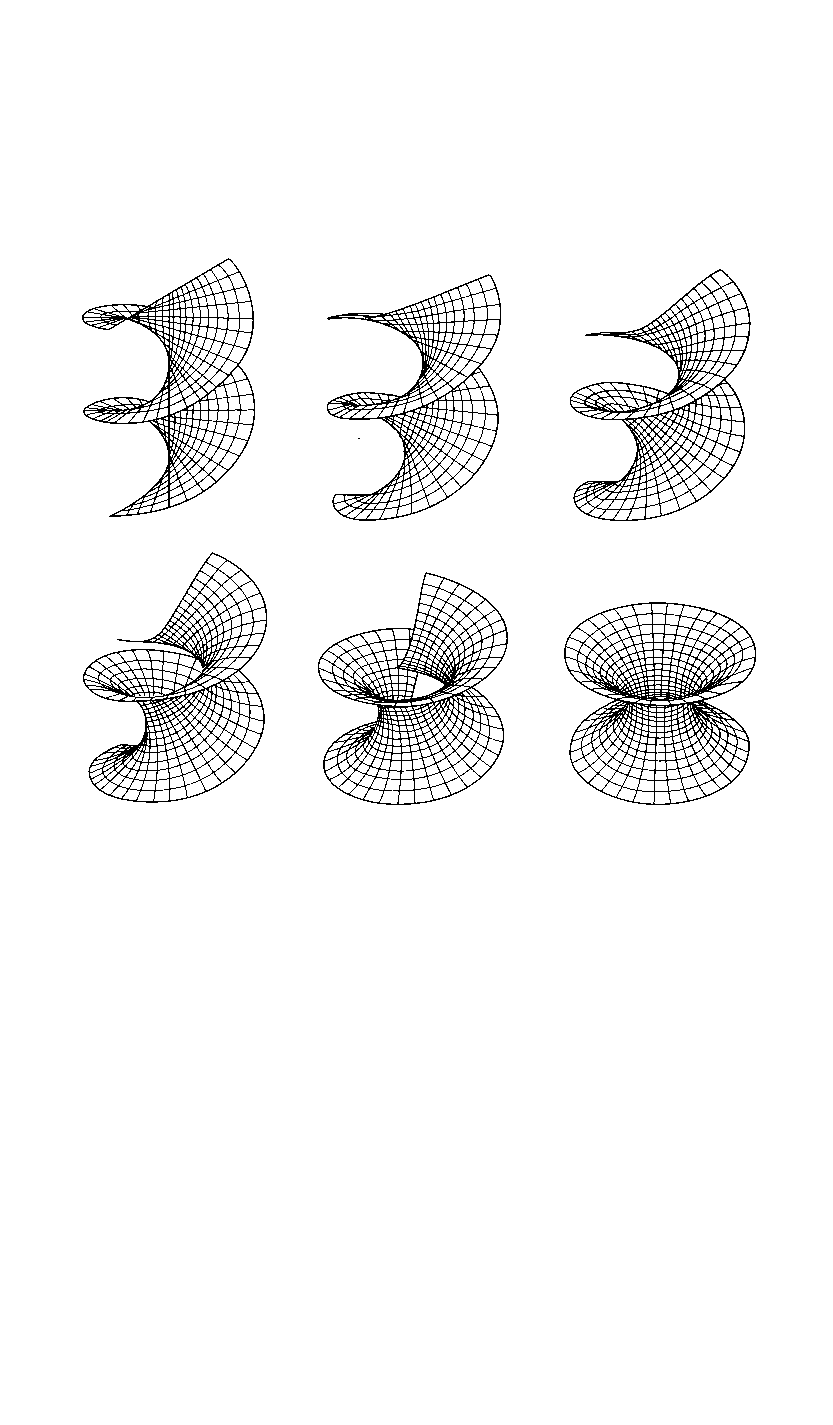
\includegraphics[scale=0.5]{figures/helicoid.pdf}
    \caption{A $1$-parameter family of minimal ($H=0$) isometric immersions of a surface connecting the helicoid (top left) to the catenoid (bottom right). From \cite{Spivak3}.}
    \label{fig:helicoid}
\end{figure}

\begin{example}[Helicoid]\label{ex helicoid}
    Let $a>0$ be a constant and consider the following map $\bf{x}:\bbR^2\to \bbR^3$:
    \[\bf{x}(s,t)=(s\cos t,s\sin t,at).\]
    Its image is called the \emph{helicoid}.\index{Helicoid} Note that the $z$-axis is contained in the surface, as is a horizontal line emanating out of each point on the $z$-axis, and this line rotates as we move up the $z$-axis.
    
    We now compute the first-order adapted frame $\frake:\bbR^2\to \bbE^3$ for the helicoid (as usual, we identify the surface with its domain in $\bbR^2$ under the parametrization). Note that 
    \begin{align}
        \bf{x}_s=&(\cos t,\sin t,0),\\
        \bf{x}_t=&(-s\sin t,s\cos t,a),
    \end{align}
    so $\bf{x}_s\perp \bf{x}_t$ and we may take 
    \begin{align}
        e_1=&\frac{\bf{x}_s}{\lVert\bf{x}_s\rVert}=(\cos t,\sin t,0), \notag\\
        e_2=&\frac{\bf{x}_t}{\lVert\bf{x}_t\rVert}=\frac{1}{\sqrt{s^2+a^2}}(-s\sin t,s\cos t,a),\label{eq 2.7 Ivey}\\
        e_3=&e_1\times e_2=\frac{1}{\sqrt{s^2+a^2}}(a\sin t,-a\cos t,s).\notag
    \end{align}
    Since $\dd\bf{x}=\bf{x}_s\dd s+\bf{x}_t\dd t=\frake^\ast(\theta^1)e_1+\frake^\ast(\theta^2)e_2$, we obtain (omitting $\frake^\ast$ from the notation from now on)
    \[\theta^1=\dd s,\quad \theta^2=\sqrt{s^2+a^2} \dd t.\label{eq 2.8 Ivey}\]
    Next, we calculate the Gauss map:
    \begin{multline}
        \dd e_3=\left(-s\left(s^2+a^2\right)^{-3/2}(a\sin t,-a\cos t,s)+(s^2+a^2)^{-1/2}(0,0,1)\right)\dd s+\\
        +(s^2+a^2)^{-1/2}(a\cos t,a\sin t,0)\dd t.
    \end{multline}
    So, using (\ref{eq 2.7 Ivey}) and (\ref{eq 2.8 Ivey}), we obtain 
    \[\omega_1^3=-a(s^2+a^2)^{-1}\theta^2,\quad \omega_2^3=-a(s^2+a^2)^{-1}\theta^1.\]
    The coefficients in front of $\theta^i$ are the principal curvatures $k_i$. We conclude that $H(s,t)=0$ and $K(s,t)=-\frac{a^2}{(s^2+a^2)^2}$. Thus, the helicoid is a umbilic-free minimal surface.
\end{example}

Being a union of disjoint straight lines, the helicoid is an example of a \emph{ruled} surface.

\begin{defn}[Ruled, developable surfaces]\index{Developable surface}\index{Ruled surface}
    A surface is called ruled if every point of the surface is contained in it along with a segment of a straight line passing through that point.

    In particular, a surface $\Sigma\subset\bbE^3$ is said to be tangential developable if it can be described as (a subset of) the union of tangent rays to a curve. (These surfaces are also called \emph{tangential surfaces}.)
\end{defn}
The following proposition clarifies what developable surfaces look like.
\begin{prop}
    Let $\gamma:\bbR\to \bbE^3$ be a regular parametrized curve with curvature and torsion $\kappa$ and $\tau$, respectively, and consider the developable surface $\bf{x}:\bbR\times \bbR_+\to \bbE^3$ defined by 
    \[\bf{x}:(u,v)\mapsto \gamma(u)+v\dot\gamma(u),\quad v>0.\]
    Then this surface has $H(u,v)=\frac{\tau(u)}{2\kappa(u)v}$ and $K\equiv 0$.
\end{prop}
\begin{proof}
    Since 
    \[\dd \bf{x}=(\dot\gamma(u)+v\ddot\gamma(u))\dd u+\dot\gamma(u)\dd v,\]
    we see that $\bf{x}$ is regular, i.e.\ $\dd f$ is of maximal rank, when $\ddot \gamma(u)$ is linearly independent from $\dot\gamma(u)$ and $v\neq 0$, i.e.\ exactly when $\gamma$ is regular. Now assume that $\gamma$ is parametrized by arclength. Then $\dot\gamma\perp\ddot\gamma$ and we can take $e_1(u,v)=\dot\gamma(u)$ and $e_2(u,v)=\ddot\gamma(u)/\lVert\ddot\gamma(u)\rVert$. Using $\dd \bf{x}=\theta^1e_1+\theta^2e_2$, we calculate 
    \[\theta^1=\dd u+\dd v,\quad \theta^2=v\kappa(u)\dd u.\]
    Note that this frame coincides with the Frenet frame of $\gamma$, so, following Example~\ref{ex serret-frenet}, we have 
    \[\dd e_3=-\tau(u)e_2\dd u.\]
    Therefore, 
    \[\omega_1^3=0,\quad \omega_2^3=\frac{\tau(u)}{\kappa(u)v}\theta^2,\]
    which leads to the asserted $H$ and $K$.
\end{proof}


\begin{example}[Catenoid]\label{ex catenoid}
    Let $a>0$ be a constant and consider the following map $\bf{x}:\bbR^2\to \bbR^3$:
    \[\bf{x}(u,v)=(a\cosh v\cos u,a\cosh v\sin u,av).\]
    Its image is called the \emph{catenoid}.\index{Catenoid}
    By choosing an adapted frame and differentiating one can compute that $H=0$, so this is a minimal surface. Now consider the map $f:\bbR^2\to \bbR^2$ given by
    \[f: (u,v)\mapsto (s,t)=(a\sinh v,u).\]
    One then shows that $f^\ast(K_{\mathrm{helicoid}})=K_{\mathrm{catenoid}}$, and of course the mean curvatures match as well. But while these two surfaces have the same $H$ and $K$, the helicoid is ruled, whereas the catenoid contains no line segments. Thus, they are not congruent.
\end{example}

Nevertheless, $H$ and $K$ are usually sufficient to determine $\Sigma$ up to congruence. Those surfaces for which this is not the case either have constant $H$ or belong to a finite-dimensional family called \emph{Bonnet surfaces}.

\begin{xca}
    A surface $\Sigma$ is called \emph{flat} if $K\equiv 0$. Show that if $\Sigma$ is flat, there exist local coordinates $x^1,x^2$ on it and an orthonormal frame $(e_1,e_2,e_3)$ such that $\theta^1=\dd x^1$, $\theta^2=\dd x^2$.
\end{xca}





\subsection{Codazzi equation}

Let us now derive the compatibility condition on $h$ by setting up a Pfaffian system. Treat $\{h_{11},h_{12},h_{22}\}$ as coordinates in $\rmS^2 \bbR^2\cong\bbR^3$ and define an \gls{eds} $\calJ\subset \Omega^{\smbullet }(P\times \SE_3\times \bbR^3)$ by
\[\calJ\coloneqq \<\theta^3,\omega_1^3-h_{11}\theta^1-h_{12}\theta^2,\omega_2^3-h_{12}\theta^1-h_{22}\theta^2\>_{\mathrm{diff}}\]
with independence condition $\theta^1\wedge\theta^2\neq 0$.
We know that along the hypothetical surface $\Sigma$, these three forms must vanish. The independence condition means that $\theta^1\wedge\theta^2$ must produce a volume form after pullback to $\Sigma$. The integral manifolds of this system are graphs of immersions $\restr{P}{U}\to \SE_3$ that are adapted frame bundles of isometric immersions $\bf{x}:U\to \bbE^3$ satisfying $j^\ast \rmI=\sfg$ and $j^\ast \wt{Q}=h$. By the Frobenius Theorem~\ref{thm 4.7.8 RS1}, the derivatives of the generators of $\calJ$ must vanish modulo $\calJ$ on $\Sigma$. First, it is easy to check that $\dd\theta^3\equiv 0 \pmod{\calJ}$. The differentials of the other two forms can be combined into a column-vector, giving the following integrability condition:
\begin{multline}
    \dd \left\{
        \begin{pmatrix}
            \omega_1^3\\\omega_2^3
        \end{pmatrix}
        -h 
        \begin{pmatrix}
            \theta^1\\\theta^2
        \end{pmatrix}
    \right\}=\\
    =-\begin{pmatrix}
        0&-\omega_1^2\\
        \omega_1^2& 0
    \end{pmatrix}\wedge 
    \begin{pmatrix}
        \omega_1^3\\\omega_2^3
    \end{pmatrix}
    -\dd h\wedge 
    \begin{pmatrix}
        \theta^1\\\theta^2
    \end{pmatrix}
    +h \begin{pmatrix}
        0&-\omega_1^2\\
        \omega_1^2& 0
    \end{pmatrix}\wedge 
    \begin{pmatrix}
        \theta^1\\\theta^2
    \end{pmatrix} \equiv 
    \\
    \equiv
    -\begin{pmatrix}
        0&-\omega_1^2\\
        \omega_1^2& 0
    \end{pmatrix}\wedge h
    \begin{pmatrix}
        \omega_1^3\\\omega_2^3
    \end{pmatrix}
    -\dd h\wedge 
    \begin{pmatrix}
        \theta^1\\\theta^2
    \end{pmatrix}
    +h \begin{pmatrix}
        0&-\omega_1^2\\
        \omega_1^2& 0
    \end{pmatrix}\wedge 
    \begin{pmatrix}
        \theta^1\\\theta^2
    \end{pmatrix}\pmod{\calJ}.
\end{multline}
Thus, $h$ must satisfy the \emph{Codazzi equation}\index{Equation!Codazzi} 
\[\left\{\dd h+\left[
\begin{pmatrix}
    0 & -\omega_1^2\\
    \omega_1^2 & 0
\end{pmatrix},h
\right]\right\} \wedge 
\begin{pmatrix}
    \theta^1\\\theta^2
\end{pmatrix}=0,\label{eq Gauss-Codazzi}
\]
where $[\,,\,]$ is the commutator of matrices. 

The proof of Gauss' Theorema Egregium~\ref{thm egregium} showed that, given a metric $\sfg$ on $\Sigma$ and an orthonormal frame $\frake$, $\frake^\ast \omega_1^2$ is uniquely determined. Thus, (\ref{eq Gauss-Codazzi}) is a system of equations for the possible fundamental forms $\rmII=h_{ij}\theta^i\otimes \theta^j\otimes e_3$ for embdeddings of $\Sigma$ into $\bbE^3$ that induce the metric $\sfg$. These equations are well-defined, since (\ref{eq Gauss-Codazzi}) is invariant under changes of the frame $\frake$. Thus, the Frobenius theorem guarantees existence, while uniqueness up to a rigid motion is guaranteed only for a fixed parametrization.

\begin{thm}[Bonnet's Fundamental Theorem of Surfaces]\index{Theorem!Bonnet's Fundamental Theorem}
    Let $U$ be an open domain in $\bbR^2$. Two parametric surfaces $\bf{x},\wt{\bf{x}}:U\to \bbE^3$ are congruent (via an element of $\SE_3$) iff they have the same first and second fundamental forms at corresponding points:
    \[\bf{x}^\ast\rmI=\wt{\bf{x}}^\ast \wt{\rmI},\quad \bf{x}^\ast\rmII=\wt{\bf{x}}^\ast \wt{\rmII}.\] 
    Moreover, if $\sfg$ and $h$ are given quadratic forms on $U$ satisfying the Gauss-Codazzi equations with $\sfg$ positive definite, then there exists an immersion $\bf{x}:U\to \bbE^3$ such that $\bf{x}^\ast  \rmI=\sfg$ and $\bf{x}^\ast  \wt{Q}=h$.
\end{thm}
Note that the immersion $\bf{x}$ needs to be specified to claim uniqueness up to congruence. If only $K$ and $H$ are given, the surface cannot be reconstructed uniquely, as we saw above.
\begin{proof}
    First we show uniqueness. Let $\bf{x}:U\to \bbE^3$ be given. Then, by following the above construction, we define the adapted frame bundle $\pi:P\to U$ consisting of triples $(p,e_1,e_2)$ where $(e_1,e_2)$ are $\rmI$-orthonormal bases for $T_p U$. There are unique $1$-forms $\theta^1,\theta^2,\omega_1^2$ such that 
    \[\pi_\ast(X)=e_1\theta^1(X)+e_2\theta^2(X),\quad X\in T_{(p,e_1,e_2)}P,\]
    and
    \[\dd\theta^1=\omega_1^2\wedge \theta^2,\quad \dd\theta^2=-\omega_1^2\wedge\theta^1.\]
    Then 
    \[\pi^\ast\rmI=\sum_{i=1}^2\theta^i\otimes\theta^i,\quad \pi^\ast \wt{Q}=\sum_{i,j=1}^2 h_{ij}\theta^i\otimes\theta^j\]
    with some uniquely determined functions $h_{ij}$. Now we define $\omega_1^3\coloneqq h_{11}\theta^1+h_{12}\theta^2$ and $\omega_2^3\coloneqq h_{12}\theta^1+h_{22}\theta^2$. Then, as we saw above, $\frake\coloneqq(\bf{x}_u,\bf{x}_v,\bf{x}_u\times \bf{x}_v)$ must satisfy 
    \[\dd \begin{pmatrix}
        \frake & \bf{x}\\
        0& 1
    \end{pmatrix}=\begin{pmatrix}
        \frake & \bf{x}\\
        0& 1
    \end{pmatrix}
    \begin{pmatrix}
        0 & -\omega_1^2 & -\omega_1^3& \theta^1\\
        \omega_1^2 & 0 & -\omega_2^3 & \theta^2\\
        \omega_1^3 & \omega_2^3 & 0 & 0\\
        0 & 0& 0& 0
    \end{pmatrix}.
    \]
    Then the $4\times 4$ matrix on the right takes values in the Lie algebra $\frakse_3$, and Cartan's Fundamental Theorem~\ref{thm 6.1 Sharpe fundamental local} guarantees uniqueness of the map $\left(\begin{smallmatrix}
        \frake & \bf{x}\\
        0& 1
    \end{smallmatrix}\right): U\to \SE_3$ up to a left multiplication by an element of $\SE_3$, which is what a congruence is.

    Existence follows from the existence part of Cartan's Fundamental Theorem, since the Gauss-Codazzi equations are equivalent to the Structure Equation for the function $\left(\begin{smallmatrix}
        \frake & \bf{x}\\
        0& 1
    \end{smallmatrix}\right)$.
\end{proof}

\begin{rem}
    We can put the Gauss-Codazzi equations in an even more suggestive form by splitting up the components of all objects into tangent and normal to $\Sigma$. Let Greek indices range only over tangent directions ($1,2$), and this time we will be careful to put the row (top) index before the column (bottom) index in $\omega^i{}_j$. Then we have the two defining equations on the adapted frame bundle $P$:
    \[\dd e_\mu=e_3\omega^3{}_\mu + e_\nu\omega^\nu{}_\mu,\quad \dd e_3=e_\mu\omega^\mu{}_3.\]
    By definition of $h$ (\ref{def h}), we have $\omega^3_\mu=h_{\mu\nu}\omega^\nu$, and therefore the system becomes 
    \[\dd e_\mu= e_3 h_{\mu\nu}\omega^\nu+ e_\nu\omega^\nu{}_\mu ,\quad \dd e_3=e_\mu\omega^\mu{}_3.\]
    The Frobenius compatibility conditions for these two equations are $\dd^2 e_\mu=0$ and $\dd^2 e_3=0$. We expand the first one, use $\dd e_3=e_\mu\omega^\mu{}_3$, and collect terms containing the same basis vector:
    \[0=\dd^2e_\mu=e_3\left(\dd \omega^3{}_\mu-\omega^\nu{}_\mu\wedge\omega^3{}_\nu\right)
    +e_\nu\left(\dd\omega^\nu{}_\mu+\omega^\nu{}_\lambda\wedge\omega^\lambda{}_\mu+\omega^\nu{}_3\wedge\omega^3{}_\mu\right),
    \]
    which is equivalent to the pair of equations 
    \begin{align}
        \dd\omega^3{}_\mu-\omega^\lambda{}_\mu\wedge\omega^3{}_\lambda=&0,\\
        \dd\omega^\nu{}_\mu-\omega^\lambda{}_\mu\wedge\omega^\nu{}_\lambda=&-\omega^\nu{}_3\wedge \omega^3{}_\mu.
    \end{align}
    It is easy to check that these equations also imply the second compatibility condition, $\dd^2 e_3=0$. 
    
    By defining $b_\mu\coloneqq \omega^3{}_\mu=-\omega^\mu{}_3\eqqcolon-b^\mu$ and $\Gamma^\nu{}_\mu\coloneqq \omega^\nu{}_\mu$, we have defining equations
    \[\begin{cases}
        \dd e_\mu=b_\mu e_3+\Gamma^\nu{}_\mu e_\nu, &\\
        \dd e_3=b^\mu e_\mu, &\text{(Weingarten)}
    \end{cases}\label{3791}\]
    and the compatibility conditions for them are
    \begin{align}
        \dd b_\mu-\Gamma^\lambda{}_\mu \wedge b_\lambda=&0 &\text{(Codazzi),}\\
        \dd \Gamma^\nu{}_\mu-\Gamma^\lambda{}_\mu\wedge\Gamma^\nu{}_\lambda=&-b^\nu\wedge b_\mu &\text{(Gauss).}
    \end{align}
    Note that the right hand side of the Gauss equation is exactly $K \omega^\nu\wedge\omega^\mu$ since $b_\mu=h_{\mu\nu}\omega^\nu$ and $K=\det h$. Thus, if these Gauss-Codazzi equations are satisfied by the second fundamental form $b_\mu$, then the defining equations (\ref{3791}) can be uniquely solved for $(e_1,e_2,e_3)$ (with some initial condition), providing a map into the orthonormal frame bundle over $\bbE^3$, and hence an isometric immersion into $\bbE^3$. In time we will identify $\Gamma^\nu{}_\mu$ with the components of a (Levi-Civita) connection on the surface and $b_\mu$ with the components of a connection on its normal bundle.
\end{rem}
















\clearpage
\section{Geometry of PDE's}\label{sec: PDEs}


This \sect\ is devoted to the second side of Cartan geometry, namely as a study of geometric structures described by systems of PDE's. Much like in the Frobenius Theorem, which is the basic special case, the goal is to reduce the problem of the existence of solutions to a certain problem of linear algebra on the $C^\infty(M)$-module of differential forms on $M$. Since linear algebra on modules is exactly what homological algebra studies, it should not come as a surprise that this \sect\ will also see our first encounter with cohomology. 

We then apply these PDE methods to solve a number of classical problems in the theory of surfaces. In doing so, we will naturally come across such fundamental objects as complex geometry (Riemann surfaces), completely integrable systems, solitons, and some of the earliest global results in differential geometry and differential topology.



\subsection{Theorems of Pfaff and Darboux}

This \subsect\ introduces a few classical normal forms of differential forms that will be useful in the subsequent discussion of PDE's. It is purely technical and can be skipped on first reading.

The integrability condition from Proposition~\ref{prop 4.7.6 RS1 pfaffian rank 1} in the special case of $\dim M=3$ was first obtained by Euler in 1755. It was Pfaff who posed, in 1814-1815, the general problem of studying PDEs of the form $\theta=0$ for $\theta\in\Omega^1(M)$ in any number of dimensions.

Let $\theta\in\Omega^1(M)$ and consider the $2$-form $\dd\theta\in\Omega^2(M)$. In local coordinates its matrix has a rank which is indepedent of the choice of coordinates. First let us assume that this rank is even and equal to $2k$. The integer $k$ is called the \emph{Pfaff rank} of $\theta$. We denote by $(\dd\theta)^l\coloneqq \dd\theta\wedge\cdots\wedge\dd\theta$ the $l$-th exterior power of $\dd\theta$. Then it is easy to see that 
\[\theta\wedge(\dd\theta)^{k}\neq 0,\quad \theta\wedge(\dd\theta)^{k+1}=0,\]
that is, $k$ is the highest integer such that $\theta\wedge(\dd\theta)^{k}$ is not identically zero. 

The integer $2k+1$ is called the \emph{class of the Pfaffian equation} $\theta=0$. Note that it is well-defined as a property of the equation because any form $f\theta$, $f\in C^\infty(M)$, has the same Pfaff rank as $\theta$. Proposition~\ref{prop 4.7.6 RS1 pfaffian rank 1} can then be restated as saying that the Pfaffian equation $\theta=0$ has integral manifolds iff $\theta$ has Pfaff rank $0$.

However, it is still useful to study equations of nonzero Pfaffian rank $k>0$. Darboux showed that instead of having true integral manifolds $S$ with $TS=\ker\theta$, such a system will have non-unique integral manifolds of dimension at most $n-k-1$ such that $TS<\ker\theta$. Darboux showed this by bringing any $1$-form to a certain \emph{normal form} (this can be seen as an analog of the Rectification Theorem for $k$-frames). The proofs of the theorems in this \sect{} are rather algebraic and unenlightening, so we direct the reader to \cite{Bryant} for details.

\begin{thm}[Pfaff normal form, odd class, Darboux 1882]
    Let $\dim M=n$ and let $\theta\in\Omega^1(M)$ have Pfaff rank $k\geq 0$. Denote the class of $\theta$ by $p\coloneqq 2k+1$. Then at any point in $M$ where $\theta\wedge(\dd\theta)^k\neq 0$ there exist local coordinates $\{x^1,\ldots,x^n\}$ and a non-vanishing smooth local function $f$ such that in the case $k>0$,
    \[\theta=f\cdot (\dd x^{n-p+1}\underbrace{-x^{n-p+2}\dd x^{n-p+3}-x^{n-p+4}\dd x^{n-p+5}-\cdots -x^{n-1}\dd x^n}_{k\text{ terms}}),\]
    and in the case $k=0$, $\theta=f \dd x^n$. The maximum possible dimension of an integral manifold through $m$ is $(n-k-1)$, and for each such manifold the above coordinates can be adjusted so that it is described by 
    \[x^{n-p+1}=x^{n-p+2}=x^{n-p+4}=\cdots=x^{n-1}=0.\]
\end{thm}

The non-uniqueness of integral manifolds in the case $k>0$ can another significant consequence. Let $S$ be the integral manifold secribed by $x^{n-p+1}=x^{n-p+2}=x^{n-p+4}=\cdots=x^{n-1}=0$. Then any other integral manifold $S'$ near $S$ on which the $n-k-1$ functions $x^1,\ldots,x^{n-p},x^{n-p+3},x^{n-p+5},\ldots,x^n$ form a coordinate system can be described by equations of the form 
\begin{align}
    x^{n-p+1}=&f(x^{n-p+3},x^{n-p+5},\ldots,x^{n}),\\
    x^{x-p+2l}=&\partial_l f(x^{n-p+3},x^{n-p+5},\ldots,x^{n}),\quad 1\leq l\leq k,
\end{align}
for some suitable function $f(y^1,\ldots,y^k)$, where $\partial_l f$ denotes the partial derivative with respect to the $l$-th argument. Thus, we can informally say that the integral manifolds of the maximal dimension $n-k-1$ are locally parametrized by arbitrary functions of $k$ variables. This implies, in particular, that there is a continuous family of local diffeomorphisms of $M$ that take integral manifolds to integral manifolds, and thus preserve the Pfaffian equation $\theta=0$ itself. Clearly they must comprise a group, and in fact this is roughly how Lie groups were originally discovered.

It is also possible that the matrix of $\dd\theta$ has odd rank, in which case the normal form is slightly different.

\begin{thm}[Pfaff normal form, even class, Darboux 1882]
    Let $\dim M=n$ and let $\theta\in\Omega^1(M)$ be such that the class of the Pfaffian equation $\theta=0$ is even and equal to $p=2k>0$. Then at any point $m\in M$ there exist local coordinates $\{x^1,\ldots,x^n\}$ and a non-vanishing smooth local function $f$ such that 
    \[\theta=f\cdot (\underbrace{x^{n-p+2}\dd x^{n-p+3}+x^{n-p+4}\dd x^{n-p+5}+\cdots +x^{n-1}\dd x^n}_{k\text{ terms}}).\]
\end{thm}

Another important theorem by Darboux provides a normal form for \emph{closed $2$-forms}.

\begin{thm}[Darboux]
    Let $\omega\in\Omega^2(M)$ be closed, $\dd\omega=0$, and let $k$ be the highest integer such that the $k$-the exterior power of $\omega$ is not identically zero:
    \[\omega^k\neq 0,\quad \omega^{k+1}=0.\]
    Then at every point where $\omega^k\neq 0$ there exist local coordinates $\{x^1,\ldots,x^n\}$, $n=\dim M$, such that 
    \[\omega=\dd x^1\wedge \dd x^2+\cdots \dd x^{2k-1}\wedge\dd x^{2k}.\]
\end{thm}

We will later prove the symplectic case of this theorem, which is just the case of $2k=n$, i.e.\ when $\omega$ is non-degenerate. By combining the three theorems above, one can further simplify the normal form for $\theta$.

\begin{thm}[Darboux]
    Let $\theta\in\Omega^1(M)$ have Pfaff rank $k$ near $m\in M$. Necessarily either $(\dd\theta)^{k+1}$ vanishes at $m$ or it is nonzero near $m$. Then there exist local coordinates $\{w^0,\ldots,w^n\}$ near $m$ such that $\<\theta\>_{\mathrm{diff}}$ is locally generated by 
    \[\wt\theta=\dd w^0+w^{k+1}\dd w^1+\cdots +w^{2k}\dd w^k\]
    (i.e.\ $\theta$ is locally a nonzero multiple of $\wt\theta$). Moreover, there exist local coordinates $\{x^0,\ldots,x^{n-1}\}$ near $m\in M$ such that
    \begin{align}
        \theta=& x^0 \dd x^1+\cdots +x^{2k}\dd x^{2k+1}, &\text{ if }(\dd\theta)^{k+1}\neq 0\text{ at }m,\\
        \theta=& \dd x^1+ x^2\dd x^3+\cdots +x^{2k} \dd x^{2k+1}, &\text{ if }(\dd\theta)^{k+1}=0 \text{ at }m.
    \end{align}
\end{thm}

Lastly, the following intuitive application of the Pfaffian normal form plays a crucial role in the foundations of thermodynamics, and now in control theory.

\begin{thm}[Caratheodory]
    Let $\theta=0$ be a Pfaffian equation on $M$ of constant Pfaff rank. Then every $m\in M$ has a neighborhood $U$ such that every point $p\in U$ is connected to $m$ by an integral curve of $\theta=0$ iff it is not fully integrable, i.e.\
    \[\theta\wedge\dd\theta\neq 0.\]
\end{thm}








\subsection{Tableaux}


We have seen that differentiating the forms that generate an \gls{eds} often reveals additional conditions that integral manifolds must satisfy. The conditions are consequences of the fact that mixed partials must commute. What we did not see was a way of telling when one has differentiated enough to find all hidden conditions. In the case of Pfaffian systems, the Frobenius Theorem stated that if the system passes a first-order test, then there are no extra conditions. The general method emerging from this theory is called \emph{Cartan's Test}.

Recall from \sect~\ref{sec: frobenius ii} that an integral manifold (or simply \emph{a solution}) of an EDS $\calI\subset\Omega^{\smbullet }(M)$ with independence condition $\omega\in\Omega^n(M)$ is an immersed $n$-fold  $i:N\to M$ such that $i^\ast\alpha=0$ for all $\alpha\in \calI$ and $i^\ast \omega\neq 0$ everywhere. The ideal $\calI$ splits into a direct sum 
\[\calI=\calI^1\oplus\cdots\oplus \calI^{\dim M},\quad \calI^p\coloneqq \calI\cap \Omega^p(M),\]
of forms of different degrees. We can also perform \emph{pullbacks} of \glspl{eds} along smooth maps in the obvious way by pulling back all forms. Finally, we say that $\calI$ is \emph{locally generated} by forms with some property if every point has an open neighborhood such that the pullback of $\calI$ to that neighborhood is generated by forms with that property.

We now define ``infinitesimal solutions''. An important concept here will be that of the Grassmann bundle $\Gr_p(E)$ of a \gls{vb} $E\to M$ defined in Example~\ref{ex associated bundles}. The most important case is the Grassmann bundle of a manifold, defined as\index{Grassmann bundle!of a manifold}
\[\Gr_p M\coloneqq \Gr_r(TM).\]

Starting with the next definition, we outline the basics of \emph{Cartan's test of involutivity} and the Cartan-K\"ahler Theorem without explaining why it works, so that we can immediately see its essence in a few simple examples. The details will become clearer in the following \subsect s.

\begin{defn}[Integral element]\label{def integral element}
    We say that $E_m\in \Gr_p(T_m M)$ is an integral element of the \gls{eds} $(\calI,\omega)$ on $M$ if $\restr{\omega}{E_m}\neq 0$ and $\restr{\alpha}{E_m}=0$. We let $\calV_m(\calI,\omega)$ denote the set of integral elements of $(\calI,\omega)$ at $m\in M$. Similarly, the set of $p$-dimensional integral elements is denoted $\calV^p_m(\calI,\omega)$. $E_m$ is called \emph{maximal} if it is not contained in a larger integral element.
\end{defn}

Obviously  $p$-dimensional integral elements are completely defined by the vanishing of elements of $\calI^p$ only.

Integral elements are the potential tangent spaces to integral manifolds, in the sense that the integral manifolds of an \gls{eds} are the immersed submanifolds $N\subset M$ such that $T_mN$ is an integral element for all $m\in N$.

\begin{defn}[Polar equations]
    Let $E_m\in\calV_m(\calI)$ be an integral element of an \gls{eds} $\calI$ on $M$ at $m\in M$. The polar equations of $E_m$ are the linear functions ($1$-forms)
    \[ \theta(\_,e_1,\ldots,e_k): T_mM\to \bbR,\quad \theta\in\calI^{k+1},\; e_1,\ldots,e_k\in E_m.\]
    They vanish on a vector $X_m$ just when the span of $E\cup \{X_m\}$ is an integral element. The set of polar equations of $E_m$ is a linear subspace of $T_m^\ast M$. If $E_m$ lies in a larger integral element $F_m$, then all polar equations of $E_m$ occur among those of $F_m$: larger integral elements have at least as many polar equations.
\end{defn}

\begin{defn}[Integral flag]\index{Integral flag}
    An integral flag of an \gls{eds} $\calI$ on $M$ is a sequence of nested integral elements at a point $m\in M$ of incrementally increasing dimensions up to some dimension $p$:
    \[0=E^0_m< E^1_m< E^2_m< \cdots< E^p_m,\quad E^k_m\in\calV^k_m(\calI).\]
    These subspaces have successively larger spaces of polar equations. The \emph{characters} $s_0,\ldots,s_p$ of the flag are the increments in dimension of the space of polar equations: $E^k_m$ has polar equations of rank $s_0+s_1+\cdots s_k$.

    Consider all flags inside a given integral element $E^p_m$. Polar equations remain linearly independent under small perturbations of the flag. A \emph{generic flag} is one with locally maximal rank polar equations, i.e.\ locally maximal character sums. Generic flags form a dense open subset of flags, as we will see. The \emph{characters of the integral element} $E^p_m$ are those of its generic flag. 
\end{defn}

All integral elements of maximum possible dimension $p$ of an \gls{eds} $\calI$ on $M$ form a subset of the Grassmann bundle $\Gr_p M$. The fundamental problem in the theory of PDE's is whether this subset is a submanifold, and to predict its dimension $p$.

\begin{defn}[Involutive integral element]\index{Involutive integral element}
    A flag $E^0_m<\cdots <E^p_m$ of integral elements of an \gls{eds} $\calI$ on $M$ \emph{predicts} the dimension $\dim M+s_1+2s_2+\cdots+p s_p$. A maximal integral element \emph{predicts} the dimension predicted by its the generic flag, and it does so \emph{correctly} if the nearby integral elements form a submanifold of the Grassmann bundle of the predicted dimension. (We will see that they always sit in a submanifold of that dimension.) A maximal-dimensional integral element which correctly predicts the dimension is \emph{involutive}. An \gls{eds} is \emph{involutive} if the generic maximal integral element is involutive.
\end{defn}

The following fundamental theorem answers the question posed above in the special case of \emph{analytic} \glspl{eds}, i.e.\ \glspl{eds} on a real-analytic manifold $M$ consisting of analytic differential forms. We provide it without proof.

\begin{thm}[Cartan-K\"ahler]\index{Theorem!Cartan-K\"ahler}\label{thm Cartan-Kahler}
    Every involutive integral element of any analytic \gls{eds} is tangent to an analytic integral manifold.
\end{thm}

\begin{example}[Lagrangian submanifolds]\index{Largangian submanifold}
    We can use the Cartan-K\"ahler Theorem to prove the existence of Lagrangian submanifolds of the complex Euclidean space $\bbC^n\cong \bbR^{2n}=\{\bf{x}+\i \bf{y}\mid \bf{x},\bf{y}\in\bbR^n\}$, whose K\"ahler form is 
    \[\theta= \dd x^1\wedge \dd y^1+\cdots +\dd x^n\wedge \dd y^n.\]
    Let $\calI$ be the \gls{eds} generated by $\theta$ on $\bbR^{2n}$. Writing spans of vectors in angle brackets, 
    \begin{center}
        \begin{tabular}{l r r} 
         Flag & Polar equations & Character \\ [0.5ex] 
         \hline
         $E^0=\{0\}$ & $\{0\}$ & $s_0=0$ \\ 
         $E^1=\<\partial_{x^1}\>$ & $\<\dd y^1\>$ & $s_1=1$ \\ 
         $\vdots $ & $\vdots $ & $\vdots $ \\ 
         $E^0=\<\partial_{x^1},\ldots,\partial_{x^n}\>$ & $\<\dd y^1,\ldots,\dd y^n\>$ & $s_n=1$ \\ 
         \hline
        \end{tabular}
        \end{center}
        This flag predicts dimension 
        \[\dim \bbR^{2n}+s_1+2s_2+\cdots ns_n=2n+1+2\cdots +n.\]
        The nearby integral elements at a given point of $M$ are parametrized by $\dd \bf{y}=A\dd \bf{x}$, which we plug into $\theta=0$ to see that $A$ can be any symmetric matrix. Therefore the space of integral elements has the correctly predicted dimension
        \[\dim\bbR^{2n}+\frac{n(n+1)}{2}.\]
        The Cartan-K\"ahler Theorem proves the existence of Lagrangian submanifolds of $\bbC^n$, with (at least) one through each point, tangent to each subspace $\dd\bf{y}=A\dd\bf{x}$, for each symmetric real matrix $A$ close to $0$.
\end{example}

We always look for integral manifolds of a particular dimension $p$. For simplicity, we can assume that our \gls{eds} contains all differential forms of degree $p+1$ and higher, which doesn't change the set of $p$-dimensional integral elements. In particular, the $p$-dimensional integral elements are then maximal. The polar equations of any maximal integral element $E^p_m$ cut out precisely $E^p_m$, i.e.\ have rank $\dim M-p$ on $E^p_m$. We encounter $s_0,\ldots,s_p$ polar equations at each increment, so the rank also equals $s_0+s_1+\cdots +s_p$:
\[s_0+s_1+\cdots s_{p-1}+s_p=\dim M-p.\label{eq final character}\]
This allows us to find $s_p$ from the other characters. For even greater simplicity, we take this as a definition for the final character $s_p$; we only pretend that our \gls{eds} contains all differential forms of degree $p+1$ and higher.


\begin{example}[Harmonic functions]
    We will prove the existence of harmonic functions on the plane with given value and first derivatives at a given point. On the jet space $M=J^1(\bbR^2,\bbR)\cong\bbR^5$ with coordinates $\{x,y,u,p_x,p_y\}$, let $\calI$ be the \gls{eds} generated by 
    \[\theta=\dd u-p_x \dd x-p_y\dd y,\quad \Theta=\dd x\wedge \dd p_y-\dd y\wedge\dd p_x.\]
    Note that 
    \[\dd\theta=\dd x\wedge \dd p_x-\dd y\wedge \dd p_y\]
    must also belong to $\calI$ by definition of an \gls{eds}. Any integral surface on which the independence condition $\dd x\wedge\dd y\neq 0$ is satisfied is locally the graph of a harmonic function $u(x,y)$ and its derivatives $u_x,u_y$.

    Each integral plane ($2$-dimensional element) $E^2$ on which $\dd x\wedge\dd y\neq 0$ is given by equations 
    \begin{align}
        \dd p_x=p_{xx}\dd x+p_{xy}\dd y,\\
        \dd p_y=p_{yx}\dd x+p_{yy}\dd y,
    \end{align}
    for a unique choice of constants $p_{xx},p_{xy},p_{yx},p_{yy}$ subject to the two conditions $p_{xy}=p_{yx}$ and $p_{xx}=-p_{yy}$. Hence, the space of integral planes at a point has dimension $2$. The space of all integral planes has dimension $\dim M+2=5+2=7$. Each vector inside the above integral plane has the form 
    \[v=\left(v^x,v^y,p_xv^x+p_yv^y,p_{xx}v^x+p_{xy}v^y,p_{yx}v^x+p_{yy}v^y\right).\]
    Each integral line $E^1$ is the span $E^1=\<v\>$ of a nonzero such vector. Compute 
    \[i_v \begin{pmatrix}
        \dd \theta \\
        \Theta
    \end{pmatrix}=
    \begin{pmatrix}
        v^x \dd p_x+v^y\dd p_y-(p_{xx}v^x+p_{xy}v^y)\dd x-(p_{yx}v^x+p_{yy}v^y)\dd y\\
        v^y\dd p_x-v^x\dd p_y+(p_{xx}v^x+p_{xy}v^y)\dd y+(p_{yx}v^x+p_{yy}v^y)\dd x
    \end{pmatrix}.
    \]
    The characters then read 
    \begin{center}
        \begin{tabular}{l r r} 
         Flag & Polar equations & Character \\ [0.5ex] 
         \hline
         $E^0=\{0\}$ & $\<\theta\>$ & $s_0=1$ \\ 
         $E^1=\<v\>$ & $\<\theta,i_v\dd\theta,i_v\Theta\>$ & $s_1=2$ \\
         \hline
        \end{tabular}
    \end{center}
    We are only interested in integral surfaces, so we set $p=2$ and compute the final character from (\ref{eq final character}). Since $\dim M=5$, the characters are $(s_0,s_1,s_2)=(1,2,0)$ with predicted dimension $\dim M+s_1+2s_2+5+2+2\cdot 0=7$. We conclude involutivity. By the Cartan-K\"ahler Theorem, harmonic functions exist near any point of the plane with prescribed value and first derivatives as that point. Moreover, as we will see below, these characters tell us that the general solution depends on $2$ functions of $1$ variable (e.g.\ a pair of boundary conditions on the value and the first derivatives).
\end{example}


\begin{example}[Complex curves in $\bbC^2$]\index{Complex curve}
    On $M=\bbC^2$ with coordinates $z=x+\i y$ and $w=u+\i v$, consider the \gls{eds} $\calI=\<\Re \phi,\Im \phi\>$, where 
    \[\phi =\dd z\wedge \dd w=(\dd x\wedge \dd u-\dd y\wedge\dd v)+\i (\dd x\wedge\dd v+\dd y\wedge \dd u).\]
    Since $\calI^1=\{0\}$, any \emph{real} curve in $\bbC^2$ is an integral manifold of $\calI$. Now consider an integral surface $N<\bbC^2$. If $\dd x$ and $\dd y$ are linearly independent in $N$, then $N$ can be localy written as a graph $(x,y,u(x,y),v(x,y))$, where $u$ and $v$ satisfy the Cauchy-Riemann system\index{Equation!Cauchy-Riemann}
    \[u_x=v_y,\quad u_y=-v_x.\]
    Thus, $N$ is an integral manifold of $\calI$ iff it is a \emph{complex curve}, i.e.\ locally a graph of a holomorphic function $f(z)=u+\i v$.
\end{example}


Note that the Frobenius case corresponds exactly to all characters starting with $s_1$ vanishing, so that the resulting \emph{complete solutions} depend only on constants, and not on arbitrary functions. Since it is not obvious whether a given \gls{eds} is a Pfaffian system or not (i.e.\ whether it can be generated by $1$-forms), we can restate the Frobenius Theorem~\ref{sec: frobenius ii} in the form of a criterion on a general \glspl{eds}.

\begin{thm}[Frobenius III]\index{Theorem!Frobenius}\label{thm frobenius iii}
    Suppose $\calI$ is an \gls{eds} on a manifold $M$. \gls{tfae}, and when they hold we call $\calI$ \emph{Frobenius}:
    \begin{enumerate}
        \item Every integral element of $\calI$ lies in a unique $p$-dimensional integral element.
        \item There is an integer such that $\calI$ has a $p$-dimensional integral element at each point of $M$ with character $s_0$ equal to that integer, and all other characters $s_1,\ldots,s_p$ vanishing.
        \item $\calI$ has an involutive $p$-dimensional integral element at each point of $M$ and is locally generated by $\dim M-p$ linearly independent $1$-forms.
        \item $\calI$ is locally generated as an algebraic ideal by $\dim M-p$ linearly independent $1$-forms.
        \item $\calI$ is locally generated by linearly independent $1$-forms $\theta^1,\ldots,\theta^q$ with $\dd\theta^i=\sum_j \gamma_j^i\wedge\theta^j$ for some local $1$-forms $\gamma^i_j$.
        \item $\calI$ is locally generated by linear independent $1$-forms. The vector fields on which all $1$-forms in $\calI$ vanish are closed under Lie bracket and span a $p$-dimensional linear subspace in each tangent space of $M$.
        \item Each point of $M$ has coordinates $x^1,\ldots,x^p,y^1,\ldots,y^q$ so that $\calI$ is locally generated by $\dd y^1,\ldots,\dd y^q$.
        \item The $p$-dimensional $\calI$-integral manifolds form the leaves of a foliation of $M$, and $\calI$ is locally generated by the $1$-forms vanishing on the leaves.
    \end{enumerate}
\end{thm}


In this \subsect\ we study \emph{linear Pfaffian systems}, which are generated by $1$-forms $\{\theta^1,\ldots,\theta^s\}$ and have the additional property that the variety of integral elements through a point $m\in M$ is an affine space. This class includes all systems of PDEs expressed as \glspl{eds} on jet spaces. One way in which a linear Pfaffian system is simpler than a general \gls{eds} is that an integral element $E_m\in\calV_n(J,\omega)_m$ passes Cartan's Test iff all integral elements at $m$ do. Meanwhile the general local analytic solvability criteria for the linearization of an arbitrary  nonlinear analytic \gls{eds} coincide with those of the full system by the implicit function theorem.


Throughout this \sect, $V$ is an $n$-dimensional vector space, and $W$ is an $s$-dimensional space. We use the index ranges $1\leq i,j,k\leq n$, $1\leq a,b,c\leq s$. $V$ has basis $\{v_i\}_{i=1}^n$ and $V^\ast$ the corresponding dual basis $\{v^i\}_{i=1}^k$; $W$ has basis $\{w_a\}_{a=1}^s$ and $W^\ast$ the dual basis $\{w^a\}_{a=1}^s$.

Let $x=x^iv_i$, $u=u^aw_a$ denote elements of $V$ and $W$, respectively. We will consider $(x^1,\ldots,x^n)$, respectively $(u^1,\ldots,u^n)$, as coordinate functions on $V$ and $W$ respectively, so that $v^i=\dd x^i$, $v_i=\partial_{x^i}$, and $w^a=\dd u^a$, $w_a=\partial_{u^a}$. Any first-order, constant-coefficient, homogeneous system of PDE's for maps $f:V\to W$ is given in coordinates by equations
\[B_a^{ri}\frac{\partial u^a}{\partial x^i}=0,\quad 1\leq r\leq R,\label{eq 5.1 Ivey}\]
where the $B_a^{ri}$ are constants. 
% For example, the Cauchy-Riemann system $u^1_{x^1}-u^2_{x^2}=0$, $u^1_{x^1}+u^2_{x^1}=0$ has $B_1^{11}=B_2^{21}=B_1^{22}=1$, $B_2^{12}=-1$, $B_1^{12}=B_2^{11}=B_1^{21}=B_2^{22}=0$.
To phrase (\ref{eq 5.1 Ivey}) in a coordinate-free manner, given a map $f:V\to W$, we define a ``Gauss map''
\begin{align}
    \gamma_f:V\to V^\ast\otimes W\cong \Hom(V,W),\\
    x\mapsto \frac{\partial f^a(x)}{\partial x^i}w_a\otimes v^i=\frac{\partial f^a(x)}{\partial x^i} \partial_{u^a}\otimes \dd x^i,
\end{align}
where we identify $T_xV\cong V$, $T_{f(x)}W\cong W$ and translate the differential to the origin. In other words, we identify $J^1_x(V,W)\slash J^0_x(V,W)$ with $W\otimes V^\ast$. More generally, we will use the identification
\[J^k_x(V,W)\slash J^{k-1}_x(V,W)\cong W\otimes \rmS^k V^\ast,\]
of the ``highest order terms of $k$-jets'' with the homogeneous $W$-valued polynomials of degree $k$ on $V$. Now, our system may be described as a subspace $B<V\otimes W^\ast$, where 
\[B=\{B_a^{ri}\partial_{x^i}\otimes\dd u^a\mid 1\leq r\leq R\}.\]
We think of $B$ as the space of equations. A map $f$ is a solution if $B$ annihilates $\gamma_f(x)$ for all $x\in V$, i.e.\ $\<b,\gamma_f(x)\>=0$ for all $x\in V,b\in B$.
$B$ is often called the space of \emph{symbol relations} (it generalizes the \emph{principal symbol} used in standard PDE terminology). We think of $B$'s annihilator $\Ann(B)\subset W\otimes V^\ast$ as the space of admissible first derivatives. In computations we will often use $\Ann(B)$ rather than $B$, so it has a special name.

\begin{defn}[Tableau]\index{Tableau}
    A tableau is a linear subspace $A\subset W\otimes V^\ast$. A tableau $A$ determines a first-order, constant-coefficient, homogenenous system of PDE's for maps $f:V\to W$, namely the system whose solutions are those maps $f$ satisfying $\gamma_f(V)\subset A$.
\end{defn}

Note that systems defined by a tableau always have solutions 
\[f(x)=f_0+A_0x,\quad f_0\in W,A_0\in A.\] 
We will be interested in what higher-order terms can appear in the Taylor series of a solution.

\begin{example}
    The equation $u^1_{x^1}+u^2_{x^2}=0$ with $W=V=\bbR^2$ has symbol relations 
    \[B=\{\dd u^1\otimes \partial_{x^1}+\dd u^2\otimes \partial_{x^2}\}\subset W^\ast\otimes V\]
    and tableau 
    \[A=\Ann(B)=\{\partial_{u^1}\otimes \dd x^1-\partial_{u^2}\otimes\dd x^2,\partial_{a^1}\otimes \dd x^2,\partial_{u^2}\otimes \dd x^1\}\subset W\otimes V^\ast.\label{eq 5.2 Ivey}\]
\end{example}

Often it will be convenient to identify $V$ with $\bbR^n$ and $W$ with $\bbR^s$ using our fixed bases to write expressions in matrix form. For example, (\ref{eq 5.2 Ivey}) becomes 
\[A=\left\{
    \begin{pmatrix}
        a&c\\b&-a
    \end{pmatrix}\middle| a,b,c\in\bbR
\right\}.\]


\begin{example}\label{ex tableau}
    \begin{enumerate}
        \item The Cauchy-Riemann system $u_{x}=v_{y}$, $u_{y}=-v_{x}$ has tableau 
        \begin{multline}
            A=\{a(\partial_{u}\otimes\dd x+\partial_{v}\otimes\dd y)+b(-\partial_{v}\otimes \dd x+\partial_{u}\otimes\dd y)\mid a,b\in \bbR\}\cong\\
            \cong \left\{
                \begin{pmatrix}
                    a& -b\\b&a
                \end{pmatrix}\middle|a,b\in\bbR
            \right\}.
        \end{multline}
        \item  The tableau $A=\{0\}$ corresponds to a Pfaffian system. The equations are $u^a_{x^i}=0$ for all $i,a$. The only solutions to this system are constants. We say that \emph{solutions depend on $s$ constants}.
        \item When $A=W\otimes V^\ast$, there are no equations and any map is a solution. We say that \emph{solutions depend on $s$ functions of $n$ variables}.
        \item Let $L^\ast\subset V^\ast$ be a $k$-dimensional linear subspace and let $A=W\otimes L^\ast$. If $L^\ast=\Span\{\dd x^1,\ldots,\dd x^k\}$, the equations are $u^a_{x^\rho}=0$, $k+1\leq \rho\leq n$, and the solutions are $u^a(x^1,\ldots,x^n)=f^a(x^1,\ldots,x^k)$, where $f^a$ are arbitrary functions. We say that \emph{solutions depend on $s$ functions of $k$ variables}. With respect to adapted bases we may write elements of $A$ in block form as $\left(\begin{smallmatrix}
            *&0
        \end{smallmatrix}\right)$, where the left block is free and the right block is zero.
        \item Let $A=Y\otimes V^\ast$, where $Y$ is a $p$-dimensional linear subspace of $W$. If $Y$ is spanned by $u^\lambda$, $1\leq \lambda\leq p$, the equations are $u^\xi_{x^i}=0$, where $p+1\leq \xi\leq s$. Solutions are 
        \begin{align}
            u^\lambda(x^1,\ldots,x^n)=&f^\lambda(x^1,\ldots,x^n),\\
            u^\xi(x^1,\ldots,x^n)=&f^\xi_0,
        \end{align}
        where $f^\lambda(x^1,\ldots,x^n)$ are arbitrary functions and the $f_0^\xi$ are constants; so, \emph{solutions depend on $p$ functions of $n$ variables and $s-p$ constants.} One may think of this tableau as a combination of the previous two. With respect to adapted bases we may write $A$ in block form as $\left(\begin{smallmatrix}
            *\\0
        \end{smallmatrix}\right)$.
    \end{enumerate}
\end{example}


\begin{example}[Orthogonal 3-webs]\index{Web}
    A \emph{triply orthogonal web} is a triple of foliations of the Euclidean space $\bbE^3$ by surfaces whose leaves are pairwise orthogonal. 

    Each leaf is perpendicular to (annihilated by) a unique unit-norm $1$-form $\eta_i$, up to a sign, which satisfies $\eta_i\wedge\dd\eta_i=0$ by the Frobenius Theorem. Let $P$ be the bundle of all orthonormal bases of the tangent spaces of $\bbE^3$, with the obvious bundle projection $\pi:P\to \bbE^3$, so that each point of $P$ has the form $p=(m,e_1,e_2,e_3)$ for some $m\in \bbE^3$ and orthonormal basis $\frake=(e_1,e_2,e_3)$ of $T_{m}\bbE^3$. The \emph{soldering $1$-form} $\theta\in \Omega^1(P;\bbR^3)$ on $P$ is defined by 
    \[\frake\cdot \theta(X)=\pi_\ast(X),\quad X\in TP,\]
    i.e.\ it outputs the components of $\pi_\ast(X)$ in the frame $\frake$. In the last \subsect\ we encountered its components $\theta^i$, and we also constructed the $1$-forms 
    $\omega^i{}_j=\<\dd e_j,e_i\>,$
    which together comprise a unique $\frakso_3$ valued $1$-form on $P$ that satisfies (part of) the Structure Equation (\ref{eq structure for surfaces}):
    \[\dd \theta=-\omega\wedge\theta,\]
    where $\omega$ acts on the vector $\theta$ as a matrix. A triply orthogonal web is precisely a global section $\frake:\bbE^3\to P$  on which $0=\theta^i\wedge \dd\theta^i$ for all $i$, hence an integral $3$-manifold of the \gls{eds} $\calI$ on $P$ generated by the closed $3$-forms 
    \[\theta^i\wedge\dd\theta^i,\quad i=1,2,3.\]
    Using the equations above, $\calI$ is also generated by three $3$-forms
    \[\omega^i{}_j\wedge\theta^i\wedge\theta^j,\quad (ij)=(12),(23),(31).\]
    The integral manifolds coframed by $\{\theta^i\}_{i=1}^3$ are locally precisely the triply orthogonal webs. The reader can find the characters: $(s_1,s_2,s_3)=(0,3,0)$, and the integral elements coframed by $\{\theta^i\}$ form a manifold of dimension $12$ (parametrized by a choice of a point of $P$ and $3\times 2=6$ coefficients determining the values of $\omega^i{}_j$). Again we conclude involution. As a result, triply orthogonal webs exist locally and depend on $3$ functions of $2$ variables.
\end{example}

\begin{hrem*}
    The classification of webs is equivalent to Cartan's equivalence problem for certain differential equations. in 1908, he posed the problem of the equivalence of two ODE's:
    \[y_x=f(x,y),\quad \text{ and }\quad Y_X=F(X,Y),\]
    with respect to coordinate transformations that don't mix the coordinates:
    \[\wh{x}=X(x),\quad \wh{y}=Y(y).\label{6914}\]
    This transformation leaves invariant the coordinate lines $x=a$, $y=b$ in the $xy$-plane as well as the integral lines of the equations. These three families of lines form a $3$-web \emph{in the plane}. Thus, the problem considered by Cartan is equivalent to classifying curvilinear $3$-webs in the plane. He distinguished $3$ classes of ODE's of the above type: those admitting a $3$-parameter group of transformations (\ref{6914}), those admitting a $1$-parameter such group, and those not admitting any such symmetries. This corresponds to $3$ classes of $3$-webs in the plane.
\end{hrem*}

In the rest of this \subsect, we will develop a test for a tableau such that if it passes, we will know exactly what initial data one should specify to determine an analytic solution. Given a tableau $A$, we can try to look for an analytic solution in the form of a power series ansatz
\[u^a(x)=p^a+p^a_i x^i p^a_{ij}x^ix^j+p^a_{ijk}x^ix^jx^k+\cdots.\]
Since the system is homogeneous with constant coefficients, $u$ is a solution iff each term satisfies the system and the series converges. As we have seen, there is no restriction on the constant terms, and the coefficients of the linear term must satisfy $p^a_i\partial_{u^a}\otimes \dd x^i\in A$. Moving on to the coefficients of the quadratic term in the series, the quadratic term must be such that $\gamma_{p^a_{ij}x^ix^j}(x)\in A$ for all $x\in V$. Thus,
\[p^a_{ij}x^i\partial_{u^a}\otimes \dd x^j \; \in A,\text{ for all }x\in V, \]
so that 
\[p^a_{ij}\partial_{u^a}\otimes \dd x^j\otimes \dd x^i \;\in A\otimes V^\ast.\]
Since mixed partials commute, $p^a_{ij}\partial_{u^a}\otimes \dd x^i\otimes \dd x^j$ is also an element of $W\otimes \rmS^2 V^\ast$; in indices this means $p^a_{ij}=p^a_{ji}$. Combining these two conditions gives 
\[p^a_{ij}\partial_{u^a}\otimes \dd x^i\otimes \dd x^j \; \in (A\otimes V^\ast)\cap (W\otimes \rmS^2 V^\ast)\eqqcolon A^{(1)},\]
where the first factor is due to the equations and the second to the commuting derivatives. The space $A^{(1)}$ is called the \emph{(first) prolongation} of $A$.

Similarly, the condition on the cubic term is 
\[p^a_{ijk}\partial_{u^a}\otimes \dd x^i\otimes\dd x^j\otimes\dd x^k\; \in(A\otimes V^\ast\otimes V^\ast)\cap (W\otimes \rmS^3 V^\ast)\eqqcolon A^{(2)},\]
and so on for all $l$. In general, we define 

\begin{defn}[Prolongation]\index{Prolongation}
    Let $V,W$ be vector spaces and $A<W\otimes V^\ast$ a subspace (a tableau). The $l$-th prolongation of $A$ is the subspace $A^{(l)}<W\otimes \rmS^{l+1}V^\ast$ defined as
    \[A^{(l)}\coloneqq (A\otimes V^{\ast\otimes l})\cap (W\otimes \rmS^{l+1} V^\ast)=(A^{(l-1)}\otimes V^\ast)\cap (W\otimes \rmS^{l+1} V^\ast).\]
\end{defn}

\begin{example}[Cauchy-Riemann system]
    Continuing Example~\ref{ex tableau}(1), we see that the space $A\otimes \bbR^2$ has the basis (omitting tensor products)
    \begin{multline}
        \{\partial_{u^1}\dd x^1\dd x^1+\partial_{u^2}\dd x^2\dd x^1,-\partial_{u^2}\dd x^1\dd x^1+\partial_{u^1}\dd x^2\dd x^1,\\
        \partial_{u^1}\dd x^1\dd x^2+\partial_{u^2}\dd x^2\dd x^2, -\partial_{u^2}\dd x^1\dd x^2+\partial_{u^1}\dd x^2\dd x^2\}.
    \end{multline}
    By collecting terms containing $\partial_{u^1}$ or $\partial_{u^2}$, we can write 
    \begin{multline}
        A\otimes\bbR^2=\{\partial_{u^1}(a\dd x^1\dd x^1+b \dd x^2\dd x^1+c\dd x^1\dd x^2+d\dd x^2\dd x^2)+\\
        +\partial_{u^2}(a\dd x^2\dd x^1-b \dd x^1\dd x^1+c\dd x^2\dd x^2-d\dd x^1\dd x^2)\mid a,b,c,d\in\bbR\}.
    \end{multline}
    To find the prolongation, we need the terms inside the parentheses to be symmetric tensors, i.e.\ $b=c$ and $a=-d$. Thus,
    \[A^{(1)}\cong \left\{
        \begin{pmatrix}
            a&b\\b&-a
        \end{pmatrix}\middle| a,b\in\bbR
    \right\}.\]
    Since we had $s_1=2$ and $s_2=0$, we conclude involutivity because $\dim A^{(1)}=s_1+2s_2$ holds. Thus, solutions of the Cauchy-Riemann system depend on two functions of one variable. Indeed, in complex analysis an analytic function is determined uniquely by its real and imaginary parts along a smooth curve. Continuing, it is similarly easy to check that the second prolongation is one-dimensional:
    \begin{align}
        A^{(2)}&=\bbR\cdot t,\\
        t&=(\partial_{u^1}+\partial_{u^2})(111)+(-\partial_{u^1}+\partial_{u^2})(112)+\\
        &\quad +(-\partial_{u^1}-\partial_{u^2})(122)+(\partial_{u^1}-\partial_{u^2})(222),
    \end{align}
    where $(ijk)$ stands for the sum of $\dd x^i\dd x^j\dd x^k$ over all distinct permutations if $i,j,k$. One more iteration confirms that $A^{(3)}=\{0\}$, so all higher prolongations vanish.
\end{example}


\begin{xca}
    \begin{enumerate}
        \item Show that $A^{(l)}$ is naturally identified with the set of solutions to the system of PDE's defined by $A$ that are homogeneous polynomials of degree $l+1$.
        \item Show that if $A^{(l)}=0$ for some $l$, then solutions depend on a finite number of constants.
    \end{enumerate}
\end{xca}

\begin{defn}
    A tableau of order $p$ is a linear subspace $A<W\otimes\rmS^p V^\ast$. It determines a homogeneous constant-coefficient system of PDE's of order $p$ for $W$-valued functions on $V$. In particular, the $(p-1)$-st prologation of a tableau (of order one) is a tableau of order $p$. For a tableau $A$ of order $p$, we define its prolongations by $A^{(l)}=(A\otimes V^{\ast \otimes l})\cap (W\otimes \rmS^{p+1}V^\ast)$.
\end{defn}

\begin{example}[Wave equation]
    The wave equation $u_{xy}=0$ may be encoded as a tableau of order two for $V=\bbR^2$, $W=\bbR$ as (omitting tensor products again)
    \[A=\{p_{11}\dd x\dd x+p_{22}\dd y\dd y\mid p_{11},p_{22}\in\bbR\}.\]
    Then 
    \[A\otimes\bbR^2_{x,y}=\<(\dd x)^3,\dd x\dd x\dd y,\dd y\dd y \dd x,(\dd y)^3\>,\]
    and the symmetric elements of this space are spanned by $(\dd x)^3$ and $(\dd y)^3$, so $\dim A^{(1)}=\dim A=2$. Clearly this continues in the same way for higher prolongations, so $\dim A^{(l)}=2$ for all $l$. This system is not involutive and no number of prolongations make it involutive. Nevertheless, it is known that the general solution is $u=\xi(x)+\eta(y)$, where $\xi$ and $\eta$ are arbitrary functions of one variable. The wave equation belongs to a special class of systems called \emph{Monge-Amp\`ere equations}, and we will need another method, called \emph{Darboux integrability}, to construct its solutions geometrically.
\end{example}





\begin{example}\label{ex first example Ivey}

Consider the tableau $A=(p_1,0,\ldots,0)$, where $p_1$ an arbitrary column vector (this is Example~\ref{ex tableau}(4) with $\dim L=1$). This tableau corresponds to equations $\partial_{x^p}u^a=0$, $2\leq \rho\leq n$. Its solutions are $u^a(x^1,\ldots,x^n)=f^a(x^1)$. In particular, specifying the values $u^a(x^1,0,\ldots,0)$ uniquely determines a solution, and all solutions are obtained this way.

We generalize to the tableau 
\begin{align}
    A=&\{(p_1^a\dd x^1+C_{2b}^a p_1^b\dd x^2+\cdots +C^a_{nb}p^b_1\dd x^n)\otimes \partial_{u^a}\mid p_1^a\in\bbR,1\leq a\leq s\}= \notag\\
    =& \{(p_1,C_2p_1,\ldots,C_np_1)\mid p_1\in\bbR^s\},\label{eq 5.5 Ivey}
\end{align}
where the $C_\rho$ are fixed $s\times s$ matrices. The symbol relations corresponding to this are 
\[B=\{\dd u^a\otimes \partial_{x^\rho}-C^a_{\rho b}\dd u^b\otimes\partial_{x^1}\mid 2\leq 2\leq n,1\leq a\leq s\},\]
and the corresponding differential equations are 
\[u^a_{x^\rho}-C^a_{\rho b}u^b_{x^1}=0,\quad \rho=2,\ldots,n.\label{eq 5.6 Ivey}\]
We saw that when $C_\rho= 0$ for all $\rho$, any convergent series with coefficients $p_1^a,p_{11}^a,p^a_{111},\ldots $ determines a solution $u$. The hope is that under some conditions the solutions to (\ref{eq 5.6 Ivey}) can be given in terms of $s$ arbitrary functions of one variable, and will see that this is the largest space of solutions one could hope for.

Assume we are given constants $p_1^a,p_{11}^a,p^a_{111},\ldots $. Then we may determine the remaining $p^a_I$ for any multi-index $I=(i_1,\ldots,i_k)$ as follows: to have $(p^a_i \partial_{u^a}\otimes \dd x^i)\in A$, the terms $p^a_\rho$ must be given by $p^a_\rho=C^a_{\rho b}p^b_1$. To have $(p^a_{ij}\partial_{u^a}\otimes \dd x^i\dd x^j)\in A^{(1)}$, the other terms are determined by the $p^a_{11}$:
\begin{align}
    p^a_{\rho 1}=&C^a_{\rho b}p^b_{11},\\
    p^a_{\rho\sigma}=&C^a_{\rho b}p^b_{\sigma 1}=C^a_{\rho b}C^b_{\sigma c}p^c_{11},\quad 2\leq \sigma\leq n.
\end{align}
These equations imply $\dim A^{(1)}\leq s$. They may lead to conflicting equations because it is also necessary that $p^a_{\rho\sigma}=p^a_{\sigma\rho}$, i.e.\ tat $C^a_{\rho b}C^b_{\sigma c}p^c_{11}=C^a_{\sigma b}C^b_{\rho c}p^c_{11}$. In other words, to ensure that no choice of $p^a_{11}$'s leads to a conflict, it is necessary that 
\[[C_\rho,C_\sigma]=0,\quad 2\leq \rho,\sigma\leq n.\]
If these commutators vanish, we are free to specify not only $p^a_{11}$ but in fact any convergent series for $u^a(x^1,0,\ldots,0)$.
\begin{prop}
    If the matrices $C_\rho$ in tableau (\ref{eq 5.5 Ivey}) commute, then there exists a unique solution to the initial value problem 
    \[\gamma_u(x)\in A\]
    with initial condition $u^a(x^1,0,\ldots,0)=f^a(x^1)$ where the $f^a$ are analytic.
\end{prop}
\begin{proof}
    The proof is immediate by majorants: each $k$-th order coefficient in the resulting power series is a product of $k$ matrices from the list $\{C_\rho\}$ and $1/k!$, so the magnitude of the term is bounded by $c^k/k!$ for some constant $c$, leading to convergence.
\end{proof}

In summary, the largest space of solutions one could hope for in a system of this form is that solutions depend on $s$ functions of $1$ variable, and whether or not this is the case can be determined just by computing $A^{(1)}$. One always has $\dim A^{(1)}\leq s$, and solutions depend on $s$ functions of one variable iff $\dim A^{(1)}=s$.
\end{example}

\begin{example}[Model involutive tableau]
    Now suppose that the tableau $A$ consists of matrices of the form 
    \[
        \begin{pmatrix}
            p^1_1  &  p_2^1 & \cdots & p^1_k & 0&\cdots &0\\
            \vdots & \vdots & \vdots & \vdots & 0 & \cdots & 0\\
            \vdots & \vdots & \vdots & p^{s_k}_k & 0 &\cdots & 0\\
            \vdots & \vdots & \vdots & 0 & 0 & \cdots &0\\
            \vdots & p_2^{s_2}& 0    & \vdots & 0 &\cdots & 0\\
            \vdots & 0 & \vdots      & \vdots & 0 &\cdots & 0\\
            p_1^{s_1}& \vdots &\vdots &\vdots &0 &\cdots &0\\
            0& \vdots & \vdots & \vdots  & 0& \cdots & 0\\
            \vdots & \vdots &\vdots &\vdots & 0 &\cdots &0\\
            0& \vdots & \vdots &\vdots & 0 &\vdots & 0
        \end{pmatrix}\label{eq 5.16 Ivey}
    \]
    Then $\dim A^{(1)}=s_1+2s_2+\cdots +ks_k$, since an element of $A^{(1)}$ is determined by a choice of $s_1$ constants $p^1_{11},\ldots,p^{s_1}_{11}$, then $2s_2$ constants $p^1_{12},\ldots,p^{s_2}_{12}, p^1_{22},\ldots,p^{s_2}_{22}$, and so on.

    The general solution of the corresponding system of PDE's is 
    \begin{align}
        u^a=f^a(x^1,\ldots,x^k),&\quad 1\leq a\leq s_k,\\
        u^a=f^a(x^1,\ldots,x^{k-1}),&\quad 1+s_k\leq a\leq s_{k-1},\\
        \vdots &\\
        u^a=f^a(x^1),&\quad 1+s_2\leq a\leq s_1,\\
        u^a=a^0_a=\const,&\quad 1+s_1\leq a\leq s,
    \end{align}
    If we generalize $A$ by inserting  linear combinations of the entries occurring above and to the left of each zero, we obtain a tableau of the same dimensions that satisfies the inequality
    \[\dim A^{(1)}\leq s_1+2s_2+\cdots +ks_k\]
    with equality iff any choice of the $s_1+2s_2+\cdots +ks_k$ constants $p^a_{ij}$ for a point in $A^{(1)}$ determines the other $p^a_{ij}$'s without conflict. Moreover, in this case $A^{(k)}$ has its maximum possible dimension for all $k$ as well, i.e.\ commutation of all second-order derivatives implies commutation of all higher-order derivatives.
\end{example}


These examples motivate the following general definition.

\begin{defn}
    Given a tableau $A<W\otimes V^\ast$ expressed in terms of bases $b=(\dd x^1,\ldots,\dd x^n)$ of $V^\ast$ and $q=(\partial_{u^1},\ldots,\partial_{u^s})$ of $W$, let $s_1(b),\ldots,s_n(b)$ be defined by 
    \begin{align}
        s_1(b)=&\; \#\text{ of indepedent entries in the first column of }A,\\
        s_1(b)+s_2(b)=&\; \#\text{ of indepedent entries in the first 2 columns of }A,\\
        \vdots &\\
        s_1(b)+\cdots +s_n(b)=&\; \#\text{ of indepedent entries in }A=\dim A.\\
    \end{align}
    Thus, $s_k(b)$ is the number of new independent variables in the $k$-th column.
\end{defn}

Now that $s_k(b)$ depends only on the (co)flag $F=(F_0>\cdots >F_n)$ of subspaces of $V^\ast$ induced by $b$, which we denote by 
\[F_j=\Ann\{\partial_{x^1},\ldots,\partial_{x^j}\}=\{\dd x^{j+1},\ldots, \dd x^n\},\]
with $F_0=V^\ast$ and $F_n=\{0\}$. Hence we can write $s_k(F)$ instead of $s_k(b)$. We define 
\[A^k(F)\coloneqq (W\otimes F_k)\cap A\]
and observe that 
\[\dim A^k(F)=s_{k+1}(F)+\cdots s_n(F).\label{eq 5.17 Ivey}\]
One can visualize $A_k(F)$ as the subspace of matrices in $A$ for which the first $k$ columns are zero, when we use the basis $b$ for $V$. In example~\ref{ex first example Ivey}, $A^1=(0)$.

\begin{defn}
    Let $A<W\otimes V^\ast$ be a tableau. Define 
    \[s_k(A)\coloneqq \max\{s_k(F)\mid F\text{ flags with }s_j(F)=s_j(A),j=1,\ldots,k-1\}.\]
    The $s_k$ are called the \emph{(reduced) characters} of $A$. They are invariants of $A$ with respect to the action of $\GL(V)\times\GL(W)$. We will call a flag $F$ an $A$-generic flag when $s_k(F)=s_k(A)$ for all $k$ (it exists by definition). We will write $s_k$ instead of $s_k(A)$ when there is no risk of confusion. Note that 
    \[\dim W=s\geq s_1\geq \cdots \geq s_n\geq 0.\]
\end{defn}

We fix an $A$-generic flag $F$ induced by a basis $b$, and will suppress further reference to it. Given $U< W\otimes \rmS^d V^\ast$, we define 
\[U_k\coloneqq U\cap (W\otimes \rmS^{n-k}\Span\{\dd x^{k+1},\ldots,\dd x^n\}).\]
Note that 
\[(A_k)^{(1)}=(A^{(1)})_k.\]

\begin{prop}[{{\cite[Prop.~5.5.3]{Ivey}}}]
    \[\dim A^{(1)}\leq s_1+2s_2+3s_3+\cdots +ns_n. \label{eq 5.18 Ivey}\]
\end{prop}
\begin{proof}
    We have the exact sequence 
    \[0\to A_k{}^{(1)}\to A_{k-1}{}^{(1)}\to A_{k-1},\]
    in which the last map is $p\mapsto i_{\partial_{x^k}}p$ (contraction with the first component of $\rmS^{n-k}V^\ast$). Thus, 
    \[\dim A_{k-1}{}^{(1)}-\dim A_k{}^{(1)}\leq \dim A_{k-1}.\]   
    Summing for $1\leq k\leq n$ (and recalling that $A_0=A$), we have 
    \[\dim A^{(1)}\leq \dim A+\dim A_1+\cdots +\dim A_{n-1},\]
    which, along with (\ref{eq 5.17 Ivey}), gives the result.
\end{proof}
\begin{defn}[Involutive tableau]
    A tableau $A<W\otimes V^\ast$ is said to be involutive if equality holds in (\ref{eq 5.18 Ivey}).
\end{defn}


For the ``model'' involutive tableau (\ref{eq 5.16 Ivey}), solutions are uniquely determined by specifying $u^\sigma(x^1,\ldots,x^k,0,\ldots,0)$ for $\sigma\leq s_k$. This motivates the following.

\begin{defn}[Level]
    Let $s_k$ be the characters of a tableau. For an integer $\sigma$ between $1$ and $s$, define the level of $\sigma$ be the largest $k$ such that $\sigma\leq s_k$. If $\sigma>s_1$, its level is defined to be $0$.
\end{defn}

For any tableau, the largest set of initial data one could hope to specify is 
\[u^\sigma(x^1,\ldots,x^k,0,\ldots,0),\text{ where }\mathrm{level}(\sigma)=k,\label{eq 5.19 Ivey}\]
with an interal manifold obtained by solving a sequence of Cauchy problems. In fact, an argument that is conceptually the same as in the examples of the previous sections yields.

\begin{thm}[Cartan-K\"ahler for tableaux {{\cite[Thm.~5.5.7]{Ivey}}}]\label{thm 5.5.7 Ivey}
    Let $A<W\otimes V^\ast$ be a tableau. Choose $A$-generic bases of $V$, $W$ which induce coordinates $x^i$ on $V$ and $u^a$ on $W$. If $A$ is involutive, then any choice of analytic functions (\ref{eq 5.19 Ivey}) determines a unique integral manifold of the system of PDE's represented by $A$ in some neighborhood of the origin.
\end{thm}

\begin{defn}
    If $A$ is an involutive tableau such that $s_l\neq 0$ but $s_{l+1}=0$, then $s_l$ is called the character of the system and the number $l$ is called the \emph{Cartan integer}.
\end{defn}

According to Theorem~\ref{thm 5.5.7 Ivey}, a solution is determined by specifying 
\begin{align}
    s_l &\text{ functions of }l\text{ variables},\\
    s_{l-1}-s_l& \text{ functions of }l-1\text{ variables},\\
    \vdots &\\
    s_1-s_2&  \text{ functions of }1\text{ variable},\\
    s-s_1 & \text{ constants.}
\end{align}

The freedom of the functions of $l$ variables is more significant than all the other choices in the sense that it provides the overwhelming majority of the Taylor coefficients at high orders. Thus we usually say that for an involutive \gls{eds} with character $s_l$ the integral manifolds \emph{depend on $s_l$ functions of $l$ variables}, and ignore the rest.

In Theorem~\ref{thm 5.5.7 Ivey} we do not necessarily obtain all solutions to an involutive system by a choice of analytic functions as specified in the theorem. We only obtain those that can be obtained by specifying \emph{noncharacteristic} initial data, that is, initial data based on a choice of an $A$-generic flag for $V^\ast$. If we choose a nongeneric flag, the corresponding Cauchy problem may not have any solutions or be undetermined, with an infinite number of solutions.

\begin{example}\label{ex 5.6.1 Ivey}
    Consider the system 
    \[u_x=v_y,\quad u_y=u_x.\label{eq 5.20 Ivey}\]
    If we pick initial data for $u,v$ along a line through the origin other than $x=\pm y$, then it extends to a unique solution to the system. But if we specify initial data along the line $y=x$, then unless $u-v=\const$, this cannot be extended to a solution. If $u-v=\const$ along $y=x$, then there are an infinite number of local extensions to a solution.
\end{example}

\begin{defn}[Symbol mapping, Characteristic variety]\label{def symbol map}
    Let $A<W\otimes V^\ast$ be a tableau. For $\alpha\in V^\ast$, define the \emph{symbol mapping} at $\alpha$ by 
    \[\sigma_\alpha:W\to (W\otimes V^\ast)\slash A,\quad w\mapsto w\otimes\alpha + A.\]
    Define the \emph{characteristic variety} of $A$, $\Xi_A\subset \bbP V^\ast$ (where $\bbP$ stands for the projectivization functor $V\mapsto V\slash \bbK^\times$ for $\bbK$-vector spaces), to be the set of all \emph{characteristic hyperplanes} (codimension $1$ subspaces) in $V$:
    \[\Xi_A\coloneqq \{[\alpha]\in \bbP V^\ast\mid \ker \sigma_\alpha\neq 0\}.\]
    We interpret $\Xi_A$ is the set of hyperplanes in $\bbP V$ for which the extension of an $(n-1)$-dimensional integral element to an $n$-dimensional one is not unique, see Theorem~\ref{thm 6.7.7 Ivey}.
\end{defn}

\begin{example}[\ref{ex 5.6.1 Ivey} continued]
    The tableau of \ref{eq 5.20 Ivey} consists of matrices of the form $\left(\begin{smallmatrix}
        a&b\\b&a
    \end{smallmatrix}\right)$. This has characters $s_1=2=\dim A$ and $s_2=0$. A lin in $V$ spanned by $\left(\begin{smallmatrix}
        x\\ y
    \end{smallmatrix}\right)$ is characteristic iff the system $ax+by=0$, $bx+ay=0$ on $a,b$ has rank below $2$. Of course, this happens only for the two lines $y=\pm x$. Thus $\Xi_A=\{[1:1],[1:-1]\}$. 
\end{example}

Even when we are only interested in real solutions of the udnerlying PDE, it is useful to consider the \emph{complex characteristic variety}
\[\Xi^\bbC_A\coloneqq \{[\alpha]\in \bbP (V^\ast)^\bbC\mid \ker \sigma_\alpha^\bbC\neq 0\},\]
where $\sigma^\bbC_\alpha:W^\bbC\to (W^\bbC\otimes (V^\ast)^\bbC)\slash A^\bbC$ is the complexification of $\sigma_\alpha$ (see Definition~\ref{def complexification}).

\begin{defn}[Determined tableau]
    A tableau $A<W\otimes V^\ast$ is called determined if $\dim \Ann(A)=\dim W=s$, i.e.\ the number of equations is the same as the number of unknowns.
\end{defn}

Let us now \emph{work over $\bbC$ and drop $\bbC$ from the notation}. We estimate the dimension of $\Xi_A$ and a modification of the degree of $\Xi_A$ in terms of the characters of $A$. We use the convention that the empty set has dimension $-1$, and denote the modified degree defined below by $\widetilde{\deg}$.

\begin{thm}[{{\cite[Thm.~5.6.12]{Ivey}}}]\label{thm 5.6.12 Ivey}
    Let $A<W\otimes V^\ast$ be a tableau. Noncharacteristic integral manifolds of the \gls{eds} induced by $A$ depend on $\widetilde{\deg}(\Xi_A^\bbC)$ functions of $\dim\Xi_A^\bbC+1$ variables.
\end{thm}






\subsection{Linear Pfaffian systems}


Recall that a Pfaffian system is an \gls{eds} on $M$ generated by $1$-forms $\theta^a\in \Omega^1(M)$, $a=1,\ldots,s$, i.e.\ 
\[\calI=\<I\>_{\mathrm{diff}}, I=\<\theta^1,\ldots,\theta^s\>.\]
We also specify $n$ $1$-forms $\{\omega^1,\ldots,\omega^n\}$,  which induce our independence condition $\omega^1\wedge\cdots\wedge\omega^n\neq 0$. We describe this problem by the pair 
\[(I,J),\quad J\coloneqq \<I\cup\{\omega^i\}_{i=1}^n\>.\]
Note that the set $\{\omega^i\}_{i=1}^n$ must be pointwise linearly independent.

\begin{defn}[Linear Pfaffian system]
    The pair $(I,J)$ is called a linear Pfaffian system if $\dd \theta^a\equiv 0\pmod{J}$ (as an algebraic ideal) for all $1\leq a\leq s$.
\end{defn}

Since $J$ is pointwise linearly independent, it can be locally completed to a local frame for $T^\ast M$ by a set of $1$-forms $\{\pi^\lambda\}_{\lambda=1}^{\dim M-n-s}$. Then, modulo $I$ (which is equivalent to the imposition of the Pfaffian equations), $\Omega^2(M)$ is locally spanned by the $2$-forms $\pi^\lambda\wedge \omega^i$ and $\omega^i\wedge\omega^j$. This means that, localy,
\[\dd\theta^a\equiv A^a_{\lambda j}\pi^\lambda\wedge\omega^j+T^a_{ij}\omega^i\wedge\omega^j \pmod{I},\label{eq def tableau+torsion}\]
for some unique set of smooth local functions $A^a_{\lambda i}$ and $T^a_{ij}$. We will also use the notation 
\[\dd\theta^a\equiv \pi^a_j\wedge\omega^j\pmod{I},\quad \pi^a_j=A^a_{\lambda j}\pi^\lambda+T^a_{ij}\omega^i.\]
The term with $A^a_{\lambda j}$ determines the \emph{tableau} (see below). The term with $T^a_{ij}$ not containing any $\pi^\lambda$'s is called \emph{apparent torsion}. We say that apparent torsion is \emph{absorbable} if it can be made zero by a proper choice of $\{\pi^\lambda\}$. If this is not possible, we say that there is \emph{intrinsic torsion} $[T]\neq 0$, where $[T]$ is the equivalence class consisting of all possible apparent torsion $1$-forms. Note that $[T]$ depends only on the space spanned by $\pi^\lambda$'s modulo $I$, so this space needs to be changed if one hopes to absorb apparent torsion. In other words, $\pi^\lambda$'s need to be modified by adding multiples of $\omega^j$'s.\index{Torsion!apparent}

\begin{rem}
    In general nonlinear \glspl{eds} $\calI$, we can perform a similar construction by letting $\pi^\lambda$'s be a pointwise completion of $\{\omega^i\}$ to a basis for $T_m^\ast M\slash \calI^1_m$. We can also let  $\{\vartheta^q\}_{q=1}^r$  be a set of (algebraic) generators for $\calI_m\slash \calI^1_m$ -- these are necessarily of degree at least $2$. Therefore there exists a decomposition 
    \[\vartheta^q=A^q_{\lambda j}\pi^\lambda\wedge\omega^j+T^q_{ij}\omega^i\wedge\omega^j + A^q_{\lambda\mu j}\pi^\lambda\wedge\pi^\mu\wedge \omega^j + T^q_{ijk}\omega^i\wedge\omega^j\wedge\omega^k+\cdots. \]
    In this case the first term $A^q_{\lambda j}\pi^\lambda$ is the tableau, whereas all the remaining terms break up into \emph{apparent torsion} consisting of terms with no $\pi^\lambda$'s in them, and \emph{nonlinearity} consisting of terms with two or more $\pi^\lambda$ wedged into them. Since in the linear case $\calI\slash \calI^1\cong \<\dd\theta^a\>_{\mathrm{alg}}$, we can pick $\vartheta^a=\dd\theta^a$, and then this description agrees with the above definitions.
\end{rem}


\begin{example}\label{ex linear pfaff}
    Let $i:M\hookrightarrow J^1(V,W)\cong V\oplus W\oplus (W\otimes V^\ast)$ be defined by a constant-coefficient homogeneous system as in the previous \subsect. Let $J^1(V,W)$ have coordinates $(x^i,u^a,p^a_i)$ and let $\theta^a=\dd u^a-p^a_i \dd x^i$, $\omega^i=\dd x^i$. As usual, we omit the pullback $i^\ast$ in notation. The pullback of the contact system to $M$ is still denoted 
    \[I=\Span\{\theta^a\},\quad J=\Span\{\theta^a,\omega^i\},\]
    and we have 
    \[\dd\theta^a\equiv -\dd p^a_j\wedge \omega^j\pmod{I}.\label{eq 6.2 Ivey}\]
    However, $\dd p^a_i$ pulled back to $M$ are not all independent. Say we choose forms $\pi^\lambda$, $\lambda=\rank J+1,\ldots,\dim M$, such that $\{\theta^a,\omega^i,\pi^\lambda\}$ are a local coframe for $M$. Since $M$ is defined by homogeneous equations $B^{ri}_a p^a_i=0$, we may choose  $\pi^\lambda$ so that 
    \[\dd p^a_i=-A^a_{\lambda i}\pi^\lambda\]
    for some constants $A^a_{\lambda i}$ such that $B^{ri}_a A^a_{\lambda i}=0$. Thus we may write (\ref{eq 6.2 Ivey}) as 
    \[\dd\theta^a\equiv A^a_{\lambda i}\pi^\lambda\wedge\omega^i \pmod{I}.\]
    Observe that $(J\slash I)_m\cong V^\ast$  and $I_m\cong W^\ast$. When we work with general linear Pfaffian systems, these will be the definitions for $V$ and $W$. The tableau is recovered by taking 
    \[A\coloneqq \Span\{A^a_{\lambda i}\partial_{u^a}\otimes \dd x^i\mid \lambda=\rank J+1,\ldots,\dim M\}< W\otimes V^\ast.\]
    As we saw in the last \subsect, if the tableau $A$ is involutive, we have local existence of integral manifolds, roughly depending on $s_l$ functions of $l$ variables, where $l$ is the Cartan integer and $s_l$ is the final character of the tableau. For an arbitrary linear Pfaffian system with no intrinsic torsion, we will define a tableau at a general point $m\in M$, and if this tableau is involutive, we will again have local existence of integral manifolds.
\end{example}


\begin{rem}\label{rem 6.3.1 Ivey}
    We can consider the more general case of \emph{non-homogeneous} constant-coefficient linear systems. Let there be constants $C^r_i$ such that the equations are of the form 
    \[B^{ri}_a p^a_i=C^r_i x^i.\]
    Then we must have $\dd p^a_i=-A^a_{\lambda i}\pi^\lambda+T^a_{ij}\omega^j$, where $A^a_{\lambda i}$ are as before, and $T^a_{ij}$ are constants which satisfy $C^r_i=B_a^{rj}T^a_{ij}$. Now we have nonzero apparent torsion:
    \[\dd\theta^a\equiv A^a_{\lambda i}\pi^\lambda \wedge \omega^i+T^a_{ij}\omega^i\wedge\omega^j\pmod{I}.\]
    It might be possible to modify $\pi^\lambda$'s by adding multiples of $\omega^j$'s to absorb the apparent torsion. We will examine this below.
\end{rem}

\begin{example}[\ref{ex linear pfaff} continued]
    If $A$ is not involutive, we need to examine third-order information. The test will be to compare a naive estimate for the dimension of $\dim A^{(2)}$ with its actual dimension (recall that $A^{(2)}$ can be interpreted as the space of admissible third-order terms in the Taylor series of a solution). 

    We start with a new system, which is the pullback of the tautological linear Pfaffian system on the second order jet space 
    \[J^2(V,W)\cong V\oplus W\oplus (W\otimes V^\ast)\oplus (W\otimes \rmS^2 V^\ast)\]
    to $\wt{M}\cong V\oplus W\oplus A\oplus A^{(1)}$. This new system is called the \emph{(first) prolongation} of $(I,J)$ on $M$.

    Recall that, in coordinates $(x^i,u^a,p^a_i,p^a_{ij})$, the contact system on $J^2(V,W)$ is generated by 
    \[\theta^a=\dd u^a-p^a_i\dd x^i,\quad \theta^a_i=\dd p^a_i-p^a_{ij}\dd x^j.\]
    We omit pullbacks $i^\ast$ along the inclusion $i:\wt{M}\hookrightarrow J^2(V,W)$ as before. In particular, note that on $\wt{M}$, only $\dim A$ of the forms $\theta^a_i$ are indepedent. 

    Writing our new system as $I=\<\theta^a,\theta^a_i\>$, we observe that $\dd\theta^a\equiv 0\mod{I}$, so our $(s+\dim A)\times n$ tableau, when represented by a matrix, will always have the first $s\times n$ block zero. We now apply Cartan's test for involutivity to this tableau. If it is involutive, then local integral manifolds exist; if not, then further prolongation is necessary.
\end{example}


Let us return to general definitions. Let $(I,J)$ be a linear Pfaffian system as above with $I=\<\theta^a\>$, $J=\<\theta^a,\omega^i\>$ and $\{\pi^\lambda\}$ such that the tableau and the torsion are defined by (\ref{eq def tableau+torsion}).

\begin{defn}[Tableau of a linear Pfaffian system]
    Fix a generic point $m\in M$. Let $V^\ast=(J\slash I)_m$ and $W^\ast=I_m$, Write $w^a=\theta^a_m$, $v^j=\omega^j_m$, and define the tableau of $(I,J)$ at $m$ by 
    \[A_m\coloneqq \{A^a_{\lambda i} w_a\otimes v^i\mid \lambda=1,\ldots,\dim M-\dim J_m\}<W\otimes V^\ast.\]
    It is indepedent of any choices made along the way. Denote the annihilator of $A$ by $B=\Ann(A)=\<B^{ri}_a w^a\otimes v_i\>< W^\ast\otimes V$. If $\dd\theta^a\equiv \pi^a_i\wedge \omega^i\pmod{I}$, then the \emph{symbol relations} of $A$ are the equations
    \[B^{ri}_a\pi^a_i\equiv C^r_j \omega^j\pmod{I},\quad r=1,\ldots,\codim A.\]
\end{defn}

In the presence of intrinsic torsion, it is impossible to choose a complement to $J_m<T^\ast_mM$ such that the apparent torsion at $m$ vanishes. In this case there are no integral elements at $x$. We now discuss these statements in coordinate-free fashion.

A change of complement $\wt{\pi}^\lambda-\pi^\lambda=e^\lambda_i \omega^i$, called \emph{contorsion}, leads to a change in apparent torsion equal to
\[\wt{T}^a_{ij}-T^a_{ij}=\frac12(A^a_{\lambda j}e^\lambda_i-A^a_{\lambda i}e^\lambda_j)\eqqcolon E^a_{ij}.\]
This motivates us to define the anti-symmetrization operator
\[\delta:W\otimes V^\ast\otimes V^\ast\to W\otimes \bigwedge^2V^\ast.\]
Given a contorsion, it computes the corresponding change in apparent torsion. Therefore, $\ker\delta$ can be (non-naturally) identified with the set of contorsions that do not change a given apparent torsion. Also note that its kernel is exactly the set of symmetric elements of $A\otimes V^\ast$, which is $A^{(1)}$. This provides a useful method for computing $A^{(1)}$ in practice using the following proposition.

\begin{prop}[{{\cite[Prop.~6.7.1]{Ivey}}}]\label{prop 6.7.1 Ivey}
    For a given tableau $A<W\otimes V^\ast$, the space of all possible sets $\{\pi^\lambda\}\pmod{I}$ of $1$-forms such that $\dd\theta^a\equiv \pi^a_i\wedge\omega^i\pmod{I}$ is an affine space modeled on the prolongation $A^{(1)}$.
\end{prop}
\begin{proof}
    Indeed, there is no ``origin'' in the space of possible sets of $1$-forms $\{\wt{\pi}_i^\lambda\}$ such that $\dd\theta^a\equiv\wt{\pi}^a_i\wedge \omega^i\pmod{I}$. We need only to identify each element of $\ker\delta$ relative to a given $\{\pi^a_i\}$ with a unique element of $A^{(1)}$. Let $\wt{\pi}^a_i\equiv\pi^a_i+p^a_{ij}\omega^j \pmod{I}$. The $\wt{\pi}^a_i$ must satisfy the symbol relations $B^{ri}_a\wt{\pi}^a_i\equiv 0\pmod{I}$. But $B^{ri}_a \wt{\pi}^a_i\equiv B^{ri}_a(\pi^a_i+p^a_{ij}\omega^j)\equiv B^{ri}_a(p^a_{ij}\omega^j)\pmod{I}$, since $\pi^a_i$ also satisfies the symbol relations. This implies $B^{ri}_ap^a_{ij}=0$ for all $j$, since the $\omega^j$ are independent, so $p^a_{ij}w_a\otimes v^i\otimes v^j\in A\otimes V^\ast$. But we also need $\wt{\pi}^a_i\wedge \omega^i\equiv \pi^a_i\wedge\omega^j+p^a_{ij}\omega^i\wedge\omega^j\equiv 0\pmod{I}$. We already have $\pi^a_i\wedge \omega^i\equiv 0\pmod{I}$, so this forces $p^a_{ij}\omega^i\wedge \omega^j=0$, which implies $p^a_{ij}=p^a_{ji}$.
\end{proof}

Since $E\coloneqq E^a_{ij}w_a\otimes v^i\otimes v^j$ lies in $\delta(A_m\otimes V^\ast)$, the space of all possible apparent torsions attainable from a given one is $\delta(A\otimes V^\ast)$. Then the \emph{intrinsic torsion} of $(I,J)$ at $m$ is defined as the equivalence class of apparent torsions differing by an action of contorsions, i.e.\ modulo the image of $\delta$:
\[[T_m]\coloneqq \left[T^a_{ij}w_a\otimes v^i\wedge v^j\right]\in \coker\delta =\left(W\otimes \bigwedge^2 V^\ast\right)\slash \delta(A_m\otimes V^\ast).\]
We thus have the defining \emph{kernel-cokernel exact sequence} for $\delta$ restricted to $A\otimes V^\ast<W\otimes V^\ast\otimes V^\ast$:
\[0\to A^{(1)}=\ker\delta \hookrightarrow \underbrace{A\otimes V^\ast}_{\text{contorsions}}\overset{\delta}{\to}\underbrace{W\otimes\bigwedge^2 V^\ast}_{\text{app.\ torsions}}\to \underbrace{\coker\delta}_{\text{int.\ torsions}}\to 0.\]
We will use the notation 
\[H^{0,2}(A_m)\coloneqq \coker\delta=\left(W\otimes \bigwedge^2V^\ast\right)\slash \delta(A_m\otimes V^\ast).\]
If $[T_m]\equiv 0$, then any apparent torsion terms we have for a specific choice of coframe are absorbable and the set of integral elements at $m$ coincides with $A^{(1)}_m$, making it an affine space (explaining the name ``\emph{linear} Pfaffian system''). For the purposes of Cartan's Test, actually carrying out the absorption is not necessary because the tableau is independent of it. If $[T_m]$ is not identically zero, we need to restrict our system to $M'\subset M$ on which $[T]\equiv 0$. On this subset we may obtain new symbol relations resulting from $\dd [T]=0$.

It is possible that $\dd[T]=0$ forces a relation among the $\omega^i$ on an open subset of $M'$. If this happens, we must restrict further to the subset $M''\subset M'$ where the $\omega^i$ are independent. If $M''$ is impty, there are no integral manifolds and we are done. In any event, restricting to $M'$ and $M''$ will in general introduce new symbol relations, which in turn could introduce more apparent torsion, and so we must repeat the above process. We have proven the following.

\begin{thm}[Cartan-K\"ahler for linear Pfaffian systems {{\cite[Thm.~6.5.6]{Ivey}}}]\label{thm 6.5.6 Ivey}
    Let $(I,J)$ be an analytic linear Pfaffian system on a manifold $M$, let $m_0\in M$ have a neighborhood $U$ such that, for all $m\in U$,
    \begin{enumerate}
        \item $[T_m]=0$;
        \item The tableau $A_m$ is involutive.
    \end{enumerate}
    Then solving a series of Cauchy problems yields integral manifolds to $(I,J)$ passing through $m_0$ that depend (in the sense discussed in the last \subsect) on $s_l$ functions of $l$ variables, where $s_l$ is the final character of the system.
\end{thm}

We interpret the Cartan-K\"ahler Theorem as saying: if there is no obstruction to having an integral element at a general point $m\in M$, then the space of integral manifolds passing through $m$ is of the same dimension as the space of integral manifolds for the corresponding linearized problem. In other words, if the linear algebra works out at the infinitesimal level, it also works out locally.

When a linear Pfaffian system $(I,J)$ satisfies the conditions of Theorem~\ref{thm 6.5.6 Ivey} at $m$, we say it is \emph{involutive} at $m$. Note that if conditions 1 and 2 are satisfies at m, then they are automatically satisfied in some neighborhood of $m$.

Let us formalize the process of prolongation. Let $\calI$ be an arbitrary \gls{eds} on a manifold $M$. Denote the points of the $n$-th Grassmann bundle $\pi:\Gr_n M\to M$ by $(p,E)$, where $m\in M$ and $E<T_mM$ is an $n$-dimensional subspace. Much like the contact system on the space of $k$-jets, $\Gr_n M$ carries a canonical linear Pfaffian system on it, whose integral manifolds are exactly the lifts $\wt{N}$ of immersed $n$-submanifolds $N^n\subset M$ to $\Gr_n M$ defined by $\wt{m}=(m,T_m N)$. This system on $\Gr_n M$ is defined by 
\[I_{(m,E)}\coloneqq \pi^\ast(\Ann (E)),\quad J_{(m,E)}\coloneqq \pi^\ast(T_m^\ast M).\]
Now let $\calV^n(\calI)\subset \Gr_n M$ be the subset (more presicely, subsheaf) of $n$-dimensional integral elements to $\calI$, whose fiber over a point $m$ is $\calV^n_m(\calI)$ as defined in Definition~\ref{def integral element}:
\[\calV^n(\calI)\coloneqq \{(m,E)\in \Gr_n M\mid \restr{\calI_m}{E}=0\}.\]
The \emph{prolongation} of $\calI$ (for $n$-dimensional integral manifolds) is the restriction of the canonical system on $\Gr_n M$ to $\calV^n(\calI)$.  If $\calI$ comes with an independence condition $\omega$, then we recall that 
\[\calV^n(\calI,\omega)\coloneqq \left\{(m,E)\in \Gr_n M\middle| \restr{\omega_m}{E}=\text{volume form}\right\}.\]
In this case we define the prolongation to be the restriction of the canonical system to $\calV^n(\calI,\omega)$.

\begin{rem}
    \begin{enumerate}
        \item The Cartan algorithm will not necessarily yield all integral manifolds of the original system, only the integral manifolds arising from well-posed Cauchy problems at general points.
        \item Each time one prolongs, there may be many different connected components of $\calV^n(\calI)$ to which one can restrict. To find all possible integral manifolds, one must carry out the algorithm on each component. The Cartan-Kuranishi Prolongation Theorem says in effect that this process terminates eventually, but gives no hint of how long it may take.
        \item How many prolongations it may take for the algorithm to terminate will generally depend on the component one is working with.
    \end{enumerate}
\end{rem}


\begin{defn}
    The Spencer cohomology groups $H^{i,j}(A)$ of a tableau $A<W\otimes V^\ast$ are defined as follows. Let 
    \[\delta_j:(W\otimes \rmS^iV^\ast)\otimes \bigwedge^j V^\ast\to W\otimes \rmS^{i-1}V^\ast\otimes \bigwedge^{j+1}V^\ast\]
    be defined by 
    \[\delta_j(f\otimes \alpha)=\dd f\wedge \alpha,\]
    where, for $f\in W\otimes \rmS^i V^\ast$, $\alpha\in \bigwedge^j V^\ast$, we define $\dd f$ by considering $f$ as an element of $\Hom(V^{\otimes i},W)$, and extend $\delta_j$ by linearity. In simpler terms, $\delta_j$ takes the last index of $f$ and anti-symmetrizes over the union of that index with the indices of $\alpha$. Now that $\delta_j(A^{(i)}\otimes \bigwedge^j V^\ast)\subset A^{(i-1)}\otimes\bigwedge^{j+1}V^\ast$.

    Define 
    \[H^{i,j}(A)\coloneqq \frac{\ker\restr{\delta_j}{A^{(i-1)}\otimes \bigwedge^jV^\ast}}{\im \restr{\delta_{j-1}}{A^{(i)}\otimes \bigwedge^{j-1}V^\ast}}.\]
\end{defn}

Let $\wt W=A\oplus W$. Then $A^{(1)}$ can be considered as a tableau in $\wt W\otimes V^\ast$ with the $W\otimes V^\ast$ block zero. Consider:
\begin{align}
    H^{0,2}(A^{(1)})=& \frac{\wt W\otimes \bigwedge^2 V^\ast}{\delta\left(A^{(1)}\otimes V^\ast\right)}\\
    =& \frac{W\otimes V^\ast\otimes \bigwedge^2 V^\ast}{\delta\left(\left((A\otimes V^\ast)\cap (W\otimes \rmS^2 V^\ast)\right)\otimes V^\ast\right)}\\
    =&H^{1,2}(A).
\end{align}
Since prolongations can be defined iteratively, this easily implies that 
\[H^{0,2}(A^{(p)})=H^{p,2}(A).\]

\begin{rem}
    The \emph{Kuranishi Prolongation Theorem} implies that after a finite number of porllongations a tableau will become involutive (perhaps by becoming empty). This implies that, for a linear Pfaffian system on an analytic manifold $M$, if $H^{p,2}(A_m)=0$ for all $p$, then there exist integral manifolds through $m$. This statement is the \emph{Goldschmidt version of Cartan-K\"ahler Theorem}. It is useful because sometimes one can show the vanishing of all groups $H^{p,2}$ without having to compute the prolongations.
\end{rem}

Now suppose $(I,J)$ has no intrinsic torsion and let $E\in\calV^n_m(I,J)$. Let $H<E$ be a hyperplace, i.e.\ $\dim H=n-1$. We address the following question: under what circumstances is $E$ the only integral $n$-plane that contains $H$?

\begin{defn}[Characteristic hyperplane]
    A hyperplace $H<E<T_mM$ is said to be characteristic if it has more than one extension to an $n$-dimensional integral element.
\end{defn}

With notation as above, we may choose the coframe so that 
\[\restr{\theta^a}{E}=\restr{\pi^a_i}{E}=0.\]
Assume moreover that $E$ is uniquely defined by these equations, that is, $\{\theta^a,\omega^i,\pi^a_i\}$ span $T_m^\ast M$ (so there are no Cauchy characteristics).

We can also choose frames so that $\restr{\omega^n}{H}=0$. Let $e_1,\ldots,e_n$ be a basis for $E$ dual to $\{\omega^i\}$. Then $v\in T_mM\setminus H$ completes $H$ to an integral $n$-plane iff 
\[\forall\Phi \in\calI^n\quad \Phi (v,e_1,\ldots,e_{n-1})=0.\label{eq 6.17 Ivey}\]
In fact, it is sufficient to require that $i_v \theta^i=0$ and to verify (\ref{eq 6.17 Ivey}) for $\Phi=\pi^a_i\wedge \omega^J$, where $J$ is any multi-index of length $n-1$ containing the index $i$. Since $i_{e_i}\pi^\lambda=0$, (\ref{eq 6.17 Ivey}) becomes 
\[i_v\pi^a_i=0,\quad  \forall a, i=1,\ldots,n-1.\label{eq 6.18 Ivey}\]
Now recall the symbol mapping from Definition~\ref{def symbol map}, defining the characteristic variety $\Xi_A$ for $A=A_m$. If $\alpha_H\in \bbP E^\ast$ corresponds to $H<E$, then $\alpha_H\in \Xi_A$ iff 
\[B^{rn}_a w^a=0\]
for some nonzero $w\in W$. In other words, $\alpha_H\in\Xi_A$ iff the tableau contains a matrix with the first $n-1$ columns zero and the last column nonzero, or equivalently, some linear combination of the $\pi^a_n$ is linearly independent from the forms in the first $n-1$ columns, so that $v$ is not uniquely determined by (\ref{eq 6.18 Ivey}). We have now proved 
\begin{thm}
    A hyperplane $H<E<T_mM$ is characteristic iff the corresponding element $\alpha_H\in\bbP E^\ast$ is in $\Xi_A$.
\end{thm}









\subsection{Applications to surfaces}


\begin{example}[Tautological system on $\SE_3\times\bbR^3_{h_{ij}}$ for surfaces in $\bbE^3$]
    The integral manifolds of this system are the first-order adapted lifts of surfaces in $\bbR^3$, together with the components of the second fundamental form $\{h_{ij}\}$, which we view as coordinates of another space $\bbR^3$.

    Let $I=\<\omega^3,\theta^3_j\coloneqq \omega^3_j-h_{jk}\theta^k\>$. Then 
    \begin{align}
        \dd \begin{pmatrix}
            \theta^3\\\theta^3_1\\\theta^3_2
        \end{pmatrix}
        \equiv& \begin{pmatrix}
            0 & 0\\
            2h_{21}\omega^2_1-dh_{11} & (h_{22}-h_{11})\omega^2_1-d h_{11}\\
            (h_{22}-h_{11})\omega^2_1-dh_{12} & -2h_{21}\omega^2_1-dh_{22}
        \end{pmatrix}\wedge 
        \begin{pmatrix}
            \theta^1\\
            \theta^2
        \end{pmatrix}\pmod{I} \notag \\
        \equiv& 
        \begin{pmatrix}
            \pi^0_1 & \pi^0_2\\
            \pi^1_1 & \pi^1_2\\
            \pi^2_1 & \pi^2_2
        \end{pmatrix}\wedge 
        \begin{pmatrix}
            \theta^1\\
            \theta^2
        \end{pmatrix}\pmod{I},
    \end{align}
    where $\pi^a_i$'s stand for the components of the matrix in the first line. The symbol relations are 
    \[\pi^0_1\equiv \pi^0_2\equiv \pi^2_1-\pi^1_2\equiv 0\pmod{I}.\]
    There is no intrinsic torsion, and $(s_1,s_2)=(2,1)$. Integral elements are given by 
    \begin{align}
        \pi^0_1=&\pi^0_2=0,\notag\\
        \pi^1_1=&a\theta^1+b\theta^2,\notag\\
        \pi^1_2=&\pi^2_1=b\theta^1+c\theta^2,\notag\\
        \pi^2_2=&c\theta^1+e\theta^2,
    \end{align}
    where $a,b,c,e$ are arbitrary. Thus, $\dim A^{(1)}=4=s_1+2s_2$, and the system is involutive. The Cartan-K\"ahler Theorem implies that integral manifolds depend on one function of two variables. This is expected since locally any surface is a graph of a function $z=f(x,y)$.
\end{example}

The next two examples are adapted from Cartan's 1945 treatise.
\begin{example}[Linear Weingarten surfaces]\label{ex Weingarten surfaces}
    Let $A,B,C\in\bbR$ with $A\neq 0$, and let $AK+2BH+C=0$ be a linear relation between functions $H,K$. We will now set up the space of general integral manifolds for first-order adapted liftings of surfaces in $\bbR^3$, together with the components of the second fundamental form, having Gauss and mean curvatures satisfying this relation.

    This is the system above restricted to a codimension one submanifold $M\subset \SE_3\times \bbR^3_{h_{ij}}$. The submanifold is defined by the equation 
    \[A(h_{11}h_{22}-h_{12}^2)+B(h_{11}+h_{22})+C=0.\]
    The differential of this equation implies that on $M$ we may write 
    \[\dd h_{12}=\alpha d h_{11}+\beta dh_{22}\]
    for some functions $\alpha,\beta$, and thus 
    \[\pi^1_2=\alpha\pi^1_1+\beta\pi^2_2.\]
    We still have no intrinsic torsion and have characters $(s_1,s_2)=(2,0)$.  This is automatically involutive because any tableau with characters $(s,\ldots,s,0)$, where $s=\dim W$, is involutive. Solutions depend on two functions of one variable. This suggests that an appropriate Cauchy problem for determining such surfaces would be to start out with a space curve (the two functions being its curvature and torsion) and then solve for a unique surface containing the curve. Cartan carries out this construction explicitly in his treatise \emph{Les Syst\`emes Ext\'erieurs et leurs Applications G\'eom\'etriques}.
\end{example} 

\begin{example}[Conformally equivalent surfaces]
    Let $(\Sigma,\sfg)$ and $(\wb\Sigma,\wb \sfg)$ be surfaces with analytic Riemannian metrics. We set up and solve the \gls{eds} for maps $\phi:\Sigma\to \wb \Sigma$ that preserve the metric up to (point-dependent) scale, i.e.\ for \emph{conformal} maps.

    Let $P=\Fr^\ast\Sigma$ denote the orthonormal coframe bundle of $\Sigma$, with coframe $\theta^1,\theta^2,\omega^2_1=-\omega^1_2$ satisfying $\dd\theta^i=-\omega^i_j\wedge \theta^j$ as usual. Similarly, let $\wb P$ denote the orthonormal coframe bundle of $\wb\Sigma$ with coframe $\wb\theta^1,\wb\theta^2,\wb\omega^2_1$. The metric on $\Sigma$ is given by the pullback of $(\theta^1)^2+(\theta^2)^2$ (tensor squares) along any section $s:\Sigma\to P$, and that on $\wb P$ by the pullback of $(\wb\theta^1)^2+(\wb\theta^2)^2$. Thus, a conformal map $\phi:\Sigma\to \wb\Sigma$ induces  a map $\Phi:P\to \wb P$ such that $\Phi^\ast \left((\wb\theta^1)^2+(\wb\theta^2)^2\right)=\lambda^2 \left((\theta^1)^2+(\theta^2)^2\right)$ for some positive function $\lambda>0$.

    \gls{wlog}, we may require that $\Phi^\ast\theta^j=\lambda\omega^j$ because we have freedom to rotate in the tangent spaces at each point. So on $M\coloneqq P\times \wb P\times \bbR_\lambda$, $\lambda>0$, let 
    \begin{align}
        I=&\<\vartheta^1\coloneqq \theta^1-\lambda\wb\theta^1,\vartheta^2\coloneqq \theta^2-\lambda\wb\theta^2\>,\\
        J=&\<\vartheta^1,\vartheta^2,\theta^1,\theta^2,\omega^2_1\>=\<\vartheta^1,\vartheta^2,\wb\theta^1,\wb\theta^2,\wb\omega^2_1\>.
    \end{align}
    We compute 
    \begin{align}
        \dd \vartheta^1 =& -\omega^1_2\wedge \theta^2-\dd\lambda\wedge\theta^1+\lambda\wb\omega^1_2\wedge\wb\theta^2,\\
        \dd\vartheta^2=&-\omega^2_1\wedge\theta^1-\dd\lambda\wedge\theta^2+\lambda\wb\omega^2_1\wedge \wb\theta^1.
    \end{align}
    Reducing modulo $I$, we obtain 
    \[\dd\begin{pmatrix}
        \vartheta^1\\
        \vartheta^2
    \end{pmatrix}
    \equiv 
    \begin{pmatrix}
        -\lambda^{-1}\dd\lambda & -(\wb\omega^2-\omega^2_1) & 0\\
        \wb\omega^2_1 -\omega^2_1 & -\lambda^{-1}\dd\lambda & 0
    \end{pmatrix}
    \wedge 
    \begin{pmatrix}
        \theta^1\\\theta^2\\\omega^2_1
    \end{pmatrix}.
    \]
    Since $-\lambda^{-1}\dd\lambda$ and $\wb\omega^2_1-\omega^2_1$ are independent modulo $J$, there is no intrinsic torsion, and we may write 
    \[A=\left\{
        \begin{pmatrix}
            a & -b & 0\\
            b & a & 0
        \end{pmatrix}
        \middle| a,b\in\bbR
    \right\}.\]
    So $(s_1,s_2)=(2,0)$ and the tableau is involutive. Solutions depend on two functions of one variable. We may make this dependence explicit as follows.

    Specify parametrized curves $\gamma:\bbR\to \Sigma$ and $\wb\gamma:\bbR\to \wb\Sigma$ and look for conformal maps $\phi$ such that $\phi\circ \gamma=\wb\gamma$. The claim is that up to constants there is a unique such map. In fact, choose an orthonormal frame $e_1,e_2$ on $\Sigma$ such that $e_1$ is tangent to $\gamma(\bbR)$, and adapt similarly on $\wb\Sigma$. Set $\lambda=\dot{\bar\gamma}/\dot\gamma$, then the map is uniquely determined up to constants.

    Conformal maps are exactly the injective holomorphic and anti-holomorphic maps between surfaces (using the complex structures induced by the metric). These are determined by their restriction to an arc, so picking parametrized arcs determines a holomorphic or anti-holomorphic map. Even without knowing the coincidence of Lie groups $\GL_1(\bbC)\cong\CO_2$, one might have guessed this by observing that the tableau $A$ is the same as the tableau for the Cauchy-Riemann equations augmented with zeros.
\end{example}

By taking $\wb\Sigma=\bbR^2$ with the standard flat metric in the last example, we get the following statement.

\begin{cor}[Korn-Lichtenstein]\label{cor isothermal coords}\index{Theorem!Korn-Lichtenstein}
    Let $\Sigma$ be a surface with an analytic Riemannian metric $\sfg$ and let $m\in\Sigma$. Then there exist local coordinates $(x,y)$ centered at $m$ such that $\sfg=\lambda^2(\dd x^2+\dd y^2)$, $\lambda\neq 0$, in some neighborhood of $m$. Such coordinates are called \emph{isothermal} and are unique up to isometry. \index{Isothermal coordinates}
\end{cor}

Note that isothermal coordinates allow us to construct canonical parametrizations of $\Sigma$ that are \emph{conformally orthonormal}, i.e.\ the corresponding coordinate vector fields $\partial_x,\partial_y$ are orthonormal only up to an overall scale. This explains why the Fundamental Theorem of surfaces required a parametrization to guarantee uniqueness: there is no natural orthonormal coordinate system on a curved surface.

\begin{defn}[Conformal structure]
    Two metric tensors $\sfg,\wt\sfg$ on a manifold $M$ are called \emph{conformally equivalent} if there exists a smooth function $\lambda\neq 0$ such that $\wt\sfg=\lambda^2 \sfg$. A conformal structure on a manifold $M$ is a conformal equivalence class of metrics $[\sfg]$.
\end{defn}

Crucially, the metric $\sfg$ on a surface cannot be recovered just from its conformal factor $\lambda^2$ in isothermal coordinates. In other words, not any two metrics on a surface are locally conformally equivalent. In the next example we characterize the intrisic information contained in $\lambda^2$.

\begin{example}[Liouville equation]\index{Equation!Liouville}
    Surfaces with given Gauss curvature have an especially simple description in isothermal coordinates. If the metric (i.e.\ First Fundamental Form) is $\sfg=\lambda^2(\dd x^2+\dd y^2)$, then, by (\ref{eq K in orthogonal coords}) with $E=G=\lambda^2$,
    \[K=-\frac{1}{\lambda^2}\left(\left(\frac{\lambda_x}{\lambda}\right)_x+\left(\frac{\lambda_y}{\lambda}\right)_y \right)=-\frac{1}{\lambda^2}(\partial_x^2+\partial_y^2)\ln\lambda.\label{eq K in isothermal coords}\]
    In particular, when $K$ is constant, the conformal factor $\varphi\coloneqq \ln\lambda$ is called the \emph{Liouville equation}:
    \[\Delta_0 \varphi+K\rme^{\varphi}=0,\label{eq liouville general}\]
    where $\Delta_0=\partial_x^2+\partial_y^2$ is the ``flat'' Laplace operator.
\end{example}

Thus, $\lambda^2$ and $K$ contain the same local information about the metric (up to the necessary boundary conditions that guarantee a unique solution of Liouville's equation). The rest of the information about the metric, namely the conformal structure, is contained in the isothermal coordinates themselves. We will later identify this information with a \emph{complex structure} on the surface.

We can also obtain the following useful formula for the mean curvature in isothermal coordinates. Since the mean curvature is not intrinsic, we need to assume a fixed isometric immersion $\bf{x}:\Sigma\to \bbE^3$.
\begin{prop}\label{prop mean curvature laplace}
    Let $\bf{x}=\bf{x}(x,y)$ be a surface parametrized by isothermal coordinates $(x,y)$ such that the metric is $\lambda^2((\dd x)^2+(\dd y)^2)$. Let $e_3$ be the unit normal vector (Gauss map) of $\Sigma$. Then 
    \[H e_3=\frac{1}{\lambda^2}\left(\bf{x}_{xx}+\bf{x}_{yy}\right).\]
\end{prop}
\begin{proof}
    Since $\bf{x}(x,y)$ is isothermal, $\<\bf{x}_x,\bf{x}_x\>=\<\bf{x}_y,\bf{x}_y\>$ and $\<\bf{x}_x,\bf{x}_y\>=0$. By differentiation, 
    \[\<\bf{x}_{xx},\bf{x}_x\>=\<\bf{x}_{yx},\bf{x}_y\>=-\<\bf{x}_x,\bf{x}_{yy}\>.\]
    Thus, 
    \[\<\bf{x}_{xx}+\bf{x}_{yy},\bf{x}_x\>=0.\]
    Similarly, 
    \[\<\bf{x}_{xx}+\bf{x}_{yy},\bf{x}_y\>=0.\]
    It follows that $\bf{x}_{xx}+\bf{x}_{yy}$ is parellel to $e_3$. Since $\bf{x}$ is isothermal, from (\ref{eq hopf differential components})
    \[H=\frac{1}{2}\frac{g+e}{\lambda^2}.\]
    Thus,
    \[2\lambda^2 H=g+e=\<e_3,\bf{x}_{xx}+\bf{x}_{yy}\>,\]
    and the result follows.
\end{proof}


\begin{example}[Minimal surfaces with given curvature]
    For simplicity, assume no umbilic points and use Darboux framings. On the orthonormal frame bundle $P\to \bbE^3$ let $K(\bf{x})$ be a given function which will be the curvature and let $k(\bf{x})=\sqrt{-K(\bf{x})}$ be the positive square root.

    Let $I=\<\theta^3,\theta^3_1,\theta^3_2\>$ and $J=\<\theta^3,\theta^3_1,\theta^3_2,\theta^1,\theta^2\>$, where we set $\theta^3_1=\omega^3_1-k\theta^1$ and $\theta^3_2=\omega^3_2+k\theta^2$. The Structure Equation modulo $I$ is 
    \[\dd\begin{pmatrix}
        \theta^3\\\theta^3_1\\\theta^3_2
    \end{pmatrix}\equiv 
    \begin{pmatrix}
        0 & 0\\
        -dk & -2k\omega^2_1\\
        -2k\omega^2_1 & dk
    \end{pmatrix}
    \wedge \begin{pmatrix}
        \theta^1\\\theta^2
    \end{pmatrix}.
    \]
    Write $\dd k=k_1\theta^1+k_2\theta^2$. The symbol relations are  (all modulo $I$)
    \begin{align}
        \pi^0_1\equiv \pi^0_2\equiv& 0 \notag\\
        \pi^2_1-\pi^1_2\equiv& 0\notag\\
        \pi^1_1+\pi^2_2\equiv& 0\notag\\
        \pi^1_1\equiv& k_1\theta^1+k_2\theta^2.
    \end{align}
    We can change bases to attempt to absorb the apparent torsion. If we rewrite our equations as 
    \[\dd\begin{pmatrix}
        \theta^3\\\theta^3_1\\\theta^3_2
    \end{pmatrix}\equiv 
    \begin{pmatrix}
        0 & 0\\
        0 & -2k\omega^2_1+k_2\theta^1\\
        -2k\omega^2_1-k_1\theta^2 & 0
    \end{pmatrix}
    \wedge \begin{pmatrix}
        \theta^1\\\theta^2
    \end{pmatrix},
    \]
    the symbol relations become 
    \begin{align}
        \pi^0_1\equiv \pi^0_2\equiv& 0 \notag\\
        \pi^2_1-\pi^1_2\equiv& -k_1\theta^1+k_2\theta^2\notag\\
        \pi^1_1\equiv \pi^2_2\equiv & 0.
    \end{align}
    This still has apparent torsion, but if we instead write 
    \[\dd\begin{pmatrix}
        \theta^3\\\theta^3_1\\\theta^3_2
    \end{pmatrix}\equiv 
    \begin{pmatrix}
        0 & 0\\
        0 & -2k\omega^2_1+k_2\theta^1-k_1\theta^2\\
        -2k\omega^2_1-k_1\theta^2+k_2\theta^1 & 0
    \end{pmatrix}
    \wedge \begin{pmatrix}
        \theta^1\\\theta^2
    \end{pmatrix},
    \]
    the symbol relations become 
    \[\pi^0_1\equiv \pi^0_2\equiv\pi^1_1\equiv\pi^2_2\equiv \pi^2_1-\pi^1_2\equiv 0\pmod{I}.\]
    We see that $(s_1,s_2)=(1,0)$ and $\dim A^{(1)}=0$, so the system is not involutive.

    We can shortcut the prolongation process by realizing that, since the system contains both $\pi^1_2\wedge\theta^1$ and $\pi^1_2\wedge\theta^2$, then $\pi^1_2$ must vanish on all integral manifolds satisfying the independence condition. Thus, we need to add $\pi\coloneqq \pi^1_2=-2k\omega^2_1+k_2\theta^1-k_1\theta^2$ to the system. Call the new system $I^+$. By counting dimensions, we see that $I^+$ will either be Frobenius at $m$ or have no integral manifold passing through $m$. We have $\dd\theta^3\equiv \dd\theta^3_1\equiv \dd\theta^3_2\pmod{I^+}$ and compute 
    \begin{align}
        \dd\pi =&\dd(-2k\omega^2_1+k_2\theta^1-k_1\theta^2)\\
        \equiv & (-k_{1,1}-k_{2,2}+\frac{k_1^2+k_2^2}{2k}+2kK)\theta^1\wedge\theta^2 \pmod{I^+},
    \end{align}
    where we have written $\dd k_j=k_{j,1}\theta^1+k_{j,2}\theta^2$. The integrability condition we have obtained can be put more simply using the Laplace-Beltrami operator defined in a Darboux frame with principal curvatures $k_1,k_2$ by
    \[\Delta f = f_{11}+f_{22}+\frac{f_1k_{2,1}-f_2k_{1,2}}{k_1-k_2}.\]
    In particular, this implies that
    \[\Delta \ln(-K)-4K=\frac{2}{k}\left(k_{1,1}+k_{2,2}-\frac{k_1^2+k_2^2}{2k}-2kK\right).\]
    The intergability condition $\dd\pi\equiv 0\pmod{I^+}$ becomes
    \[\Delta\ln(-K)=4K.\]
\end{example}

In summary:
\begin{thm}[Ricci]
    Let $(\Sigma,\sfg)$ be a surface with a Riemannian metric. Let $K$ be its curvature function. Away from umbilic points, $\Sigma$ is minimal and isometrically immersed in $\bbR^3$ iff $K<0$ and $\Delta\ln (-K)=4K$. If $K$ is not constant, then there is a one-parameter family of such immersions, up to congruence.
\end{thm}








\subsection{Cauchy characteristics}


\begin{defn}[Killing vector fields]
    Let $\calI$ be an \gls{eds} on $M$. A vector field $X\in\fX(M)$ is an infinitesimal symmetry, or a Killing vector field, of $\calI$ if 
    \[\Lie_X (\calI)\subset \calI.\]
    Since $\Lie_X$ is natural with respect to wedge products and exterior derivatives, it suffices to show that $\Lie_X \theta^a\in \calI$ for a set $\{\theta^a\}$ of \emph{differential} generators of $\calI$. The set of all Killing vector fields automatically forms a Lie subalgebra of $\fX(M)$.
\end{defn}

Given an integral manifold $N_0$ of an \gls{eds} $\calI$ on $M$, a Killing vector field $X$ can be used to obtain a one-parameter family of integral manifolds: let $F_t$ denote the flow of $X$ and 
\[N_t\coloneqq F_t(N_0).\label{eq 7.3 Ivey}\]
It is easy to see that, as long as the flow is well-defined, $N_t$ is a smooth integral manifold of $\calI$. 

\begin{rem}
    Cartan initiated the classification of \glspl{eds} whose symmetries depend on arbitrary functions (thus forming infinite-dimensional Lie algebras). Determining the symmetries usually amounts to solving an overdetermined system of differential equations, so most of the time the Lie algebra of symmetries is empty. An interesting exception is the Pfaffian system $\<\dd y-p\dd x,\dd p-q\dd x,\dd z-q^2\dd x\>_{\mathrm{diff}}$ on $\bbR^5$ with coordinates $x,y,z,p,q$. In this case the symmetries form a $14$-dimensional Lie algebra isomorphic to the split form of the exceptional Lie algebra $\frakg_2$. In his famous ``five variables paper'' Cartan proved that this is the largest possible Lie algebra of symmetries for a rank three Pfaffian system with generic derived flag on a 5-dimensional manifold.
\end{rem}

Unfortunately, enumerating the Killing vector fields for a given system of PDE's is usually harder than solving the system itself. We direct the reader to \cite{Olver} for a detailed exploration of this subject.

\begin{defn}[Cauchy characteristics]
    Let $\calI$ be an \gls{eds} on $M$. A vector field $X\in\fX(M)$ is a Cauchy characteristic vector field of $\calI$ if 
    \[i_X (\calI)\subset \calI.\]
    Since $i_X$ is a $\wedge$-derivation, it suffices to show that $i_X\theta\in\calI$ for a set $\{\theta^a\}$ of \emph{algebraic} generators of $\calI$. Since Cauchy vector fields are preserved by multiplications by arbitrary scalar function, we can talk of \emph{Cauchy characteristic line fields}. Since $\calI$ is a differential ideal, each Cauchy characteristic vector field is automatically a Killing vector field. Moreover, Cauchy characteristic vector fields also form a Lie subalgebra of $\fX(M)$ (exercise).
\end{defn}

The condition for finding Cauchy characteristics is thus algebraic, which makes them much easier to find than other Killing vector fields. And while Killing vector fields preserve the set of integral manifolds, for Cauchy characteristics a stronger statement holds.

\begin{prop}[{[\cite[Prop.~7.1.8]{Ivey}]}]\label{prop 7.1.8 Ivey}
    Let $N_0$ be an integral $n$-manifold for an \gls{eds} $\calI$ and let $X$ be a Cauchy characteristic vector field transverse to $N_0$. Let $N_t$ be as in (\ref{eq 7.3 Ivey}), and let $S$ be the $(n+1)$-dimensional union of $N_t$'s. Then $S$, when smooth, is an integral manifold of $\calI$.
\end{prop}
\begin{proof}
    Assume $\dim N_0=1$, so $N_0$ is an integral curve with $X$ transverse to it. In order for $S$ to be smooth, we must restrict $t$ to an open interval of values for which $X$ is transverse to $N_t$. Let $\omega\in\calI^2$ and let $Y$ be tangent to one of the $N_t$. Then $\omega(X,Y)=(i_X\omega)(Y)=0$ because $i_X\omega\in\calI$.  This easily generalizes to higher dimensionality of $N_0$ by replacing $Y$ with a local frame for $N_t$.
\end{proof}

\begin{example}[Surfaces in $\bbE^3$]\label{ex 7.1.10 Ivey}
    Recall tbat the integral manifolds of $\calI=\<\theta^3\>_{\mathrm{diff}}$ on the orthonormal frame bundle $\SE_3\to \bbE^3$   are the first-order adapted lifts of surfaces $\Sigma\subset\bbE^3$. This system admits a Cauchy characteristic vector field as follows.

    Let $\{E_j,E^i_j\}$ be a global frame for $TP$ dual to the one given by the entries of the Maurer-Cartan form $\{\theta^j,\omega^i_j\}$. Expand $X=X^jE_j+X^j_i E^i_j$. Then $i_X\theta^3=0$ implies that $X_3=0$ and 
    \[i_X \dd\theta^3=i_X(-\omega^3_1\wedge\theta^1-\omega^3_2\wedge\theta^2)=X_1\omega^3_1-X^1_3\theta^1+X_2\omega^3_2-X^2_3\theta^2\]
    implies that $X=X^1_2 E^2_1$. We can pick $X=E^2_1$, which geneates rotations of the frame in the $\{e_1,e_2\}$-plane. Now, Proposition~\ref{prop 7.1.8 Ivey} implies that any intgeral surface for $\calI$ may be ``thickened'' to an integral $3$-manifold using the Cauchy characteristic.
\end{example}


\begin{example}[A first-order PDE]
    Let $(x^1,x^2,u,p_1,p_2)$ be the usual coordinates on $J^1(\bbR^2,\bbR)$. The equation 
    \[u_t=u_x\] 
    is equivalent to the \gls{eds} obtained by restricting the canonical contact system to the smooth hypersurface $M$ defined by $p_2=p_1$. We will use $x=x^1,t=x^2,p=p_1$, and $u$ as coordiantes on $M$, where the system is generated algebraically by 
    \[\theta\coloneqq \dd u-p(\dd x+\dd t),\quad \dd\theta=-\dd p\wedge(\dd x+\dd t).\]
    Suppose 
    \[X=a\partial_x+b\partial_t+c\partial_p+e\partial_u\]
    is a Cauchy characteristic vector field on $M$. Then $i_X\theta=0$ implies $e=(a+b)p$. Then $i_X\dd \theta\equiv 0$ modulo $\theta$ implies that $c=a+b=0$. Hence,
    \[X=\partial_x-\partial_t\]
    up to a multiple. Integral surfaces of $\calI$ are constructed by translating integral curves along curves where $u,p$, and $x+t$ are constant.
\end{example}

\begin{example}[First-order PDE]
    Let $x^1,\ldots,x^n,u,p_1,\ldots,p_n$ be the usual coordinates on $J^1(\bbR^n,\bbR)$, and consider the PDE 
    \[F(u,x^1,\ldots,x^n,p_1,\ldots,p_n)=0.\label{eq 7.4 Ivey}\]
    Let $M\subset  J^1$ be the subset defined by this equation. To ensure that $M$ is a smooth manifold, and the equation is genuinely of first order, assume that $\partial_{p_i}F\neq 0$ for some $i$ at each point of $M$.

    Let $\theta$ be the pullback to $M$ of the contact form $\dd u-p_1\dd x^1-\cdots-p_n\dd x^n$. The solutions of the PDE are in 1-to-1 correspondence with integral $n$-manifolds $N\subset M$ of the Pfaffian system generated by $\theta$ with the independence condition $\dd x^1\wedge \cdots\wedge\dd x^n\neq 0$.

    Because $\dim M=2n$, $\theta\wedge (\dd\theta)^n=0$. Differentiating (\ref{eq 7.4 Ivey}) gives 
    \[0=\dd F=F_{x^i}\dd x^i+F_{p_j}\dd p_j+F_u\dd u\equiv (F_{x^i}+F_up_i)\dd x^i+F_{p_j}\dd p_j\mod\theta.\]I
    It follows that $\theta\wedge (\dd\theta)^{n-1}\neq 0$ at each point. By the Pfaff normal form, there are local coordinates on $M$ such that $\theta$ is a nonzero multiple of 
    \[\dd y^1+y^2\dd y^3+\cdots +y^{2n-2}\dd y^{2n-1}.\label{eq 7.5 Ivey}\]
    Thus, $X=\partial_{y^{2n}}$ gives a Cauchy characteristic. In coordinate-free language, it can be described as the unique vector field, up to multiple, such that $i_X(\theta\wedge(\dd\theta)^{n-1})=0$.

    $X$ allows us to reduce the PDE to an ODE. We do this by choosing an integral $(n-1)$-manifold $L$ of $\calI$ (corresponding to some initial data), and then using the flow of $X$ to get an integral $n$-manifold. If $F$ may be solved for $p_n$, then $X$ is transverse to the hyperplanes $x^n=\const$. Thus, we obtain a starting manifold $L$ by letting $x^n=C$, $u=f(x^1,\ldots,x^{n-1})$ for an arbitrary function, and $p_i=\partial_{x^i}f$. To obtain a solution to the original PDE we only need to integrate the ODE system corresponding to the flow of $X$.
\end{example}

\begin{xca}
    Relation~\ref{eq 7.5 Ivey} lets us locally solve for one of the $\dd p_i$'s in terms of the others, $\dd x^j$, and $\theta$. Using this, compute $\dd\theta\mod \theta$ on $M$ of dimension $2n$ and conclude that $\theta\wedge(\dd\theta)^{n-1}\neq 0$.
\end{xca}

All Cauchy characteristics (vector fields) together span a well-defined distribution $\calA(\calI)< TM$ given by 
\[\calA(\calI)_m\coloneqq \{X\in T_mM\mid i_X(\calI)\subset \calI\},\quad m\in M.\]
The rank of $\calA(\calI)$ is upper semicontinuous on $M$ (in an open neighborhood of $m$ it can only decrease), so we can restrict to an open set on which it is constant. The dual of $\calA(\calI)$ is a Pfaffian system that we define next.

\begin{defn}[Retracting system of $\calI$]
    Let $\calI$ be an \gls{eds} on $M$ with characteristic distribution $\calA(\calI)$. The retracting space, or Cartan system, of $\calI$ is the Pfaffian system $\calC(\calI)<T^\ast M$ defined by 
    \[\calC(\calI)_m\coloneqq \{\theta\in T^\ast_m M\mid i_X\theta=0 \text{ for all }X\in \calA(\calI)_m\}.\]
    Since the space of sections $\Gamma^\infty(\calA(\calI))$ (taken locally) is closed under Lie brackets of vector fields, $\calC(\calI)$ is closed under $\dd$, so it is Frobenius.\footnote{Because $\dd\theta(X,Y)=-\theta([X,Y])$ for $\theta\in\Gamma^\infty(\calC(\calI))$ and $X,Y\in\Gamma^\infty(\calA(\calI))$.} By the Frobenius Theorem, there exist local coordinates $x^1,\ldots,x^n$ on a neighborhood $U$ such that $\restr{\calC(\calI)}{U}=\<\dd x^1,\ldots,\dd x^n\>_{C^\infty(U)}$.
\end{defn}

In what follows we work on a local neighborhood $U\subset M$ where everything above holds and we let $\Omega^{\smbullet}_\Delta$ denote the subalgebra of $\Omega^{\smbullet}(U)$ spanned by wedge products of (local) sections of $\Delta<T^\ast U$ with each other. The following proposition characterizes the retracting space in a way that explains its name.

\begin{prop}
    The retracting space $\calC(\calI)<T^\ast M$ is the smallest Frobenius system such that $\Omega^{\smbullet}_{\calC(\calI)}$ contains a set of algebraic generators of $\calI$.
\end{prop}
\begin{proof}
    Let $D<T^\ast M$ be a Frobenius system such that there exist a finite collection of forms $\psi_1,\ldots,\psi_k\in \Omega^{\smbullet}_D$ which generate $\calI$ algebraically. Then any $\xi\in \calI$ can be written as
    \[\xi=\sum_{i=1}^k \beta_i\wedge \psi_i.\]
    Let $X$ be a vector field annihilated by $D$. Then $i_X \xi=\sum_i (i_X \beta_i)\wedge\psi_i$, which belongs to $\calI$. Hence $X\in\Gamma^\infty(\calA(\calI))$. Since $X$ and $\xi$ are arbitrary, we conclude that $\calC(\calI)\subset D$.

    Furthermore, the smallest such $D$ cannot be larger than $\calC(\calI)$. For, suppose $\calC(\calI)$ has co-rank $l>0$ within $D$, and let $\pi_1,\ldots,\pi_l$ be linearly independent $D$-valued forms with $\pi_i\notin \calC(\calI)$. Partition the generators for $\calI$ into $\varphi_1,\ldots,\varphi_k\in \Omega^{\smbullet}_{\calC(\calI)}$, plus generators $\psi_1,\ldots,\psi_n$ involving the $\pi_i$'s. If $X$ is any vector in $\calA(\calI)$, and $\psi_1$ has the lowest degree among the $\psi$'s, then $i_X\psi_1$ must be expressible in terms of the $\varphi_i$'s. In particular, any term in $\psi_1$ involving one of the $\pi_i$'s may be omitted since that term already is generated by the $\varphi_j$'s. It follows that we may take all generators to be in $\Omega^{\smbullet}_{\calC(\calI)}$.
\end{proof}

This means that we can calculate the retracting space by finding a minimal set of algebraic generators for the ideal.

\begin{xca}
    Consider an \gls{eds} generated by a single $\theta\in\Omega^1(M)$. Show that the rank of $\calC(\calI)$ is $2k+1$, where $k$ is the Pfaff rank, i.e.\ the highest integer such that $\theta\wedge (\dd\theta)^k$ is not identically zero.
\end{xca}

If $\calC(\calI)$ has constant rank $k$,  then the maximal integral manifolds of $\calC(\calI)$ form a foliation of $M$ by smooth manifolds of codimension $k$. In some cases, the leaf space of this foliation is a manifold, called the \emph{quotient by the Cauchy characteristics}.

\begin{example}[Example~\ref{ex 7.1.10 Ivey} continued]\label{ex 7.1.10 Ivey contd}
    For our tautological \gls{eds} for lifts of surfaces, $\calC(\calI)$ is the Frobenius system on $\SE_3$ spanned by $\theta^1,\theta^2,\theta^3,\omega^3_1,\omega^3_2$. Integral curves of $\calC(\calI)$ form a foliation of $\SE_3$. The leaf space for this foliation is a 5-dimensional homogeneous space which we identify with $S(T\bbE^3)$, the unit sphere bundle of the tangent bundle of $\bbE^3$, by letting $m$ be the basepoint and $e_3$ the unit vector in $T_m\bbE^3$.
\end{example}

In the above example, the leaf space is a manifold. Generally, whenever the leaf space is a smooth manifold, the original \gls{eds} $\calI$ can be factored to give a well-defined equivalent \gls{eds} $\wt\calI$ on the quotient manifold such that $\calI=\<\pi^\ast\wt\calI\>_{\mathrm{alg}}$, where $\pi$ is the leaf quotient map. For the proof of this fact we direct the reader to \cite[Prop.~7.1.20]{Ivey}.














\subsection{Hyperbolic second-order EDS}\label{sec: hyperbolic EDS}


We now consider a general second-order PDE for a function of two variables as an \gls{eds}. We use the standard coordinates $(x,y,z,p,q,r,s,t)$ on $J^2(\bbR^2,\bbR)$ and contact forms 
\[\theta_0=\dd z-p \dd x-q\dd y,\quad \theta_1=\dd p-r\dd x-s\dd y,\quad \theta_2=\dd q-s\dd x-t\dd y.\]
Suppose the PDE takes the form 
\[F(x,y,z,p,q,r,s,t)=0\label{eq 7.10 Ivey}\]
and that this equation defines a smooth submanifold $M^7<J^2(\bbR^2,\bbR)$, and that at least one of the partial derivatives $F_r,F_s,F_t$ is nonzero at each point of $M$, and say that $F$ is \emph{regular} when these assumptions hold. Regularity ensures that $\theta_0,\theta_1,\theta_2$ restrict to be linearly independent on $M$, and that the projection $\pi:M\to J^1(\bbR^2,\bbR)$ is a smooth submersion at each point. 

Let $I$ be the Pfaffian system spanned by the restrictions of $\theta_1,\theta_2,\theta_3$ to $M$, Since $\dd\theta_0\equiv 0\pmod{I}$, the ideal $\calI=\<I\>_{\mathrm{diff}}$ is generated algebraically by the $2$-forms 
\[\dd\theta_1=-(\dd r\wedge \dd x+\dd s\wedge \dd y),\quad \dd\theta_2=-(\dd s\wedge\dd x+\dd t\wedge\dd y).\]
Near any point in $M$, one can obtain $1$-forms $\pi_1,\pi_2,\pi_3$ such that 
\begin{align}
    \dd\theta_1\equiv &-(\pi_1\wedge \dd x+\pi_2\wedge\dd y )\pmod{I} \\
    \dd\theta_2\equiv & -(\pi_2\wedge\dd x+\pi_3\wedge\dd y) \pmod{I}
\end{align}
and such that they satisfy the symbol relation 
\[F_r\pi_1+F_s\pi_2+F_t\pi_3\equiv 0\pmod{I}.\label{eq 6.15 Ivey}\]
For example, if $F_r\neq 0$, we may choose 
\begin{align}
    \pi_1=& \dd r+\frac{F_rD_xF-F_sD_yF}{F_r^2}\dd x+\frac{D_y F}{F_r}\dd y,\\
    \pi_2=&\dd s+\frac{D_y F}{F_r}\dd x,\\
    \pi_3=&\dd t.
\end{align}
where $D_xF=F_x+pF_z+rF_p+sF_q$ and $D_yF=F_y+qF_z+sF_p+tF_q$.

Let $u\in M$ and let $E\in \calV^2(\calI)$ be an integral $2$-plane at $u$. If we use the bases $\{\theta_0,\theta_1,\theta_2\}$ for $W^\ast=I_u$ and $\{\dd x,\dd y\}$ for $E^\ast\cong V^\ast=(J\slash I)_u$, then (\ref{eq 6.15 Ivey}) shows that the tableau has the form 
\[A_u=
    \left\{
\begin{pmatrix}
    0 & 0\\
    a & b\\
    b& c
\end{pmatrix}
    \middle| aF_r(u)+bF_s(u)+cF_t(u)=0
    \right\}<W\otimes V^\ast.
\]

Applying Cartan's Test to the tableau shows that such systems are involutive with solutions depending locally on $s_1=2$ functions of one variable. Although there is usually no explicit way to describe the solutions in terms of these functions, we will see several examples where such description exists when we discuss Darboux's method.

A nonzero covector $\xi=\xi_1\dd x+\xi_2\dd y$ belongs to the characteristic variety of $\calI$ iff 
\[ F_r\xi_1^2+F_s\xi_1\xi_2+F_t\xi_2^2=0.\label{eq 7.11 Ivey}\]
Thus, the characteristic directions are the null lines of this quadratic form.

\begin{defn}[Elliptic, hyperbolic, parabolic PDE]
    The PDE (\ref{eq 7.10 Ivey}) is called elliptic, hyperbolic or parabolic according  to whether the determinant $F_rF_t-\frac{1}{4}F_s^2$ of the quadratic form is positive, negative or zero, respectively.
\end{defn}


In this section we assume that $\calI$ is hyperbolic, and the elliptic case can be dealt with similarly by using complex-valued forms. Note that (\ref{eq 7.11 Ivey}) implies that a linear combination of the system's $2$-forms is congruent, modulo $I$, to a decomposable $2$-form with $\xi$ as one of the factors. (A form is called \emph{decomposable} if it is a wedge product of $1$-forms; note that not every form is decomposable even locally.)\index{Decomposable form} Therefore, when the PDE is hyperbolic, there are two linearly independent decomposable $2$-forms in the ideal that are independent of the $\theta$'s. We may choose linearly independent forms $\pi_1,\pi_2,\omega_1,\omega_2$ that are not in $\calI^1$, such that $\pi_1\wedge\omega_1$ and $\pi_2\wedge\omega_2$ are these decomposable forms in $\calI^2$, and $\omega_1\wedge\omega_2\neq 0$ is the independence condition. In order to simplify the tableau, we may also choose new forms $\wt\theta_1,\wt\theta_2$ in $\calI^1$ so that 
\[\dd\wt\theta_1\equiv -\pi_1\wedge\omega_1,\quad \dd\wt\theta_2\equiv -\pi_2\wedge\omega_2\pmod{I}.\label{eq 7.12 Ivey}\]
(However, this is not immediately necessary.)

At each point of an integral surface for $\calI$, the tangent vectors to the surface that are annihilated by $\omega_1$ and $\omega_2$ are characteristic in the sense defined above. Moreover, since each $\pi_i$ pulls back to the surface to be a multiple of $\omega_i$, each such vector is annihilated by all of the forms of one of the following two \emph{characteristic systems}:
\[\calM_1\coloneqq \<\theta_0,\theta_1,\theta_2,\pi_1,\omega_1\>,\quad \calM_2\coloneqq \<\theta_0,\theta_1,\theta_2,\pi_2,\omega_2\>.\]
Each integral surface is foliated by integral curves of $\calM_1$ and by integral curves of $\calM_2$. In order to distinguish them from Cauchy characteristics, these curves are sometimes called \emph{Monge characteristics}.

\begin{rem}
    If $F_r\neq 0$, then $\xi=\dd y-m\dd x$ belongs to the characteristic variety iff $m$ is a root of the quadratic equation 
    \[F_rm^2-F_sm+F_t=0.\label{eq 7.13 Ivey}\]
    Assuming that this has distinct roots $m_1,m_2$, the decomposable $2$-forms in $\calI$ are 
    \[(\dd y-m_1\dd x)\wedge (\pi_2+m_2\pi_3),\quad (\dd y-m_2\dd x)\wedge (\pi_2+m_1\pi_3),\]
    where $\pi_i$ are as above.
    If the PDE (\ref{eq 7.10 Ivey}) is \emph{quasilinear} (i.e.\ the highest-order derivatives enter linearly), then the equation (\ref{eq 7.13 Ivey}) only involves $x,y,z,p,q$. More generally, we say that a second-order PDE for one function of two variables has \emph{first-order characteristics} if there exists a rank $3$ Pfaffian system on $J^1(\bbR^2,\bbR)$ whose pullback to $M$ is contained in one of the characteristic systems of $\calI$. This is the case when (\ref{eq 7.10 Ivey}) is a Monge-Amp\`ere equation, which we will consider below. The existence of first-order characteristics is intrinsic to the system, since $J^1(\bbR^2,\bbR)$ is the quotient of $M$ by the foliation dual to the retracting space of $I$'s first derived system.
\end{rem}
As a final remark, we can generalize the notion of Monge characteristics to systems which have structure equations similar to (\ref{eq 7.12 Ivey}).

\begin{defn}
    An \gls{eds} is hyperbolic of class $k$ if near any point it is algebraically generated by $k$ independent $1$-forms and two decomposable $2$-forms with no common factors.
\end{defn}

Thus, the retracting space of such a system has dimension $k+4$. For this reason, a hyperbolic \gls{eds} of class $k$ may be assumed to be defined on a $(k+4)$-dimensional manifold. This generalization will be useful for studying hyperbolic PDE's because the prolongation of a hyperbolic system of class $k$ is hyperbolic of class $k+2$. Hyperbolic systems of even class arise when we consider PDE's for two functions of two variables.









\subsection{Darboux's method}

We now turn to \emph{Darboux's method}, which gives a recipe for solving certain second-order PDE's using ODE techniques. If the equation passes a certain test, we may specify two arbitrary functions of one variable, and construct (some) solutions by solving systems of ODE's. The test is carried out by calculating the derived flag for each of the characteristic systems defined above.


\begin{defn}[Derived system]
    Let $I<T^\ast M$ be a Pfaffian system of constant rank. The derived system $I^{(1)}$ of $I$ is the subbundle spanned by $I$-valued forms whose exterior derivatives modulo $I$ vanish. More explicitly, let $\delta:\Gamma^\infty(I)\to \Gamma^\infty\left(\bigwedge^2(T^\ast M\slash I)\right)$ be defined by $\delta(\theta)=\dd\theta\mod I$. Because $\delta$ is $C^\infty(M)$-linear, it is induced by a \gls{vb} morphism from $I$ to $\bigwedge^2(T^\ast M\slash I)$. Since the coefficients of $\delta$, when expressed in matrix form, are smooth, its rank is upper semicontinuous, so we may restrict to an open set in $M$ on which it has constant rank. On this open set, we define $I^{(1)}\coloneqq \ker\delta$. If $I^{(1)}=I$, then $I$ is Frobenius; otherwise, $I^{(1)}$ is smaller. In that case, we define a sequence of systems interatively by $I^{(k+1)}=(I^{(k)})^{(1)}$, until $I^{(N)}$ is either Frobenius or rank zero. The \emph{derived flag} is 
    \[I=I^{(0)}> I^{(1)}>\cdots >I^{(N)},\]
    and $N$ is the \emph{derived length}.
\end{defn}

Note that this notation clashes with that for prolongations. Thus, for the rest of this \subsect, we use $I',I''$, etc.\ for prolongations. The dimensions of the spaces in the derived flag are differential invariants that classify Pfaffian systems. These dimensions satisfy certain systems of inequalities, see \cite{Bryant}.

\begin{example}
    On $\bbR^4$ with coordinates $(u,v,x,y)$ let $I$ be spanned by 
    \[\theta_1\coloneqq \dd y-v\dd x,\quad \theta_2\coloneqq \dd v+x\dd u.\]
    Since $\dd\theta_1\equiv x\dd u\wedge \dd x\pmod{I}$ and $\dd\theta_2=\dd x\wedge\dd u$, then $\theta^{(1)}$ is spanned by 
    \[\omega\coloneqq \theta_1+x\theta_2=\dd y+x\dd v-v \dd x+x^2\dd u.\]
    Since $\dd\omega=2\dd x\wedge\theta_2$, $I^{(1)}$ is not Frobenius. Hence the derived flag terminates in $I^{(2)}=0$.
\end{example}


The generic Pfaffian system of rank $2$ on a $4$-dimensional manifold has derived length $2$. Such systems are said to define an Engel structure. Engel's normal form shows that all such systems are locally diffeomorphic. By contrast, a generic Pfaffian system of rank $3$ in $5$ variables has derived length two but contains no Frobenius system. Unlike Engel structures, such systems are not all locally diffeomorphic to each other. Their classification was the subject of Cartan's ``five variables'' paper. 


Let $\calI$ be the \gls{eds} we constructed for the PDE (\ref{eq 7.10 Ivey}) for one function of two variables. On any integral surface of $\calI$ satisfying the independence condition, the Monge characteristic curves form two foliations which are transverse at each point of the surface. Suppose one characteristic system $\calM_i$ happens to contain two linearly independent $1$-forms that are exact derivatives:
\[\dd W,\dd X\in\calM_i.\]
Then $W$ and $X$ are both constant along the integral curves of $\calM_i$ (such functions are called \emph{Riemannian invariants} for the PDE). It follows that $W,X$ are functionally related on the integral surface. If we suppose that $\<\dd W,\dd X\>\subset \calM_i$ is linearly independent from $I$, we can assume that, say, $\dd X$ restricts to be nonzero on an open set in the integral surface. Then $W$ must be some function of $X$ on the surface. When both characteristic systems have these properties, the functions may be arbitrarily specified and used to construct a solution.


\begin{example}[Hyperbolic Liouville equation]\label{ex 7.3.6 Ivey}
    For the hyperbolic Liouville equation $z_{xy}=\rme^z$ ((\ref{eq liouville general}) with $K=-1$ and $\Delta$ replaced by the wave operator in ``lightcone coordinates'' $(x,y)\mapsto (x+y,x-y)$), the Pfaffian system $I$ is defined by \index{Equation!Liouville}
    \[
    \begin{matrix}
        \theta_0=\dd z-p\dd x-q\dd y,\\
        \theta_1=\dd p-r\dd x-\rme^z\dd y,\\
        \theta_2=\dd q-\rme^z\dd x-t\dd y,
    \end{matrix}    
    \;\;\text{with}\;\;
    \begin{matrix}
        \dd\theta_1\equiv -(\dd r-p\rme^z \dd y)\wedge \dd x\\
        \dd\theta_2\equiv -(\dd t-q\rme^z \dd x)\wedge \dd y
    \end{matrix}\pmod{I}.
    \]
    The characteristic system $\calM_1$ contains two exact derivatives, $\dd x$ and $\dd (r-\frac12 p^2)$, the latter obtained by adding multiples of $\dd x$ and $\theta_1$ to $\dd r-p\rme^z\dd y$. Similarly, $\dd y$ and $\dd(t-\frac12 q^2)$ are in $\calM_2$. Hence, 
    \[r-\frac12 p^2=f(x),\quad t-\frac12 q^2=g(y)\label{eq 7.14 Ivey}\]
    for some functions that depend on the particular solution of Liouville's equation defining our integral surface. Again, we may use these functions to determine the solution. For, if we choose $f$ and $g$ arbitrarily, and then restrict $\calI$ to the codimension-two submanifold defined by (\ref{eq 7.14 Ivey}), then the restriction is a Frobenius system. This means that we can solve for $z(x,y)$ by solving systems of ODE's. In this example, we can solve the system 
    \[z_x=p,\quad p_x=f(x)+\frac12 p^2\label{eq 7.15 Ivey}\]
    and a similar system in the $y$-direction, and be guaranteed by the Frobenius condition that we have generated a solution to the original PDE.
\end{example}

\begin{defn}[Darboux-integrable system]\index{Darboux integrability}
    A hyperbolic \gls{eds} $\calI=\<I\>_{\mathrm{diff}}$ is said to be Darboux-integrable if each characteristic system $\calM_i$ contains a Frobenius system $\Delta_i$ of rank two that is independent from $I$.
\end{defn}

\begin{prop}[{{\cite[Prop.~7.3.8]{Ivey}}}]\label{prop 7.3.8 Ivey}
    Let $\calI$ be a Darboux-integrable \gls{eds} on $M$. Let $W_1,W_2,X_1,X_2$ be functions defined on an open set $U\subset M$ such that $\dd W_i,\dd X_i\in \Delta_i$ for $i=1,2$. Let $f_1,f_2$ ve arbitrary smooth functions and let $N\subset U$ be the codimension-$2$ submanifold defined by $W_i=f_i(X_i)$. Then $\restr{\calI}{N}$ is Frobenius.
\end{prop}
\begin{proof}
    Since $\calM_i=I\oplus\Delta_i$, then on $U$ the image $\delta(I)$ is spanned by $\dd W_1\wedge\dd X_1$ and $\dd W_2\wedge \dd X_2$.
\end{proof}


\begin{example}[\ref{ex 7.3.6 Ivey} continued]
    We saw that the hyperbolic Liouville equation is Darboux-integrable. Now, to obtain a solution, it seems that we must solve Ricatti differential equations (\ref{eq 7.15 Ivey}) for $p$ and $q$. There is no general formula for solutions of Ricatti equations in quadratures. However, since $f(x)$ is arbitrary, we may make convenient choices for the form of $f(x)$. In particular, if we set $f(x)=F'(x)-\frac12 F(x)^2$, then $F(x)$ is another solution of the Ricatti equation that $p$ satisfies. The standard trick is to notice that $v=1/(p-F(x))$ satisfies a linear differential equation. Solving that equation using an integrating factor leads to 
    \[p=\frac{X''}{X'}-\frac{2X'}{X+Y'},\]
    where $X$ and $Y$ are arbitrary functions of $x$ and $y$, respectively, and $F(x)=X''/X'$. Integrating gives 
    \[z=\ln \frac{2X(x)'Y(y)'}{(X(x)+Y(y))^2.}\label{eq Liouville general solution}\]
    This is the general solution to Liouville's equation $z_{xy}=\rme^z$.
\end{example}

Note that the definition of Darboux integrability applies to hyperbolic of arbitrary rank. For example, a second-order PDE for $z(x,y)$ may become Darboux-integrable after prolonging $k$ times. Then, as before, the Pfaffian system becomes a Frobenius system of rank $2k+3$ when restricted to submanifolds of the form $U=f(X)$, $V=g(Y)$, where $\{\dd U,\dd X\}$ and $\{\dd V,\dd Y\}$ are the rank $2$ systems described in the definition. 

The problem of classifying which second-order PDE's become Darboux-integrable after a finite number of prolongations has a long history and is still a subject of current research. One of the earliest results in this area is Lie's proof that the only equations of the form $s=f(u)$ that are Darboux-integrable after a finite number of prolongations are those with $f(u)=\exp(au+b)$. Another significant early result was Goursat's classification of quasilinear equations $s=f(x,y,u,p,q)$ that are Darboux-integrable without prolongation. 








\subsection{(*) Monge equations}

Here we present an application of the derived flag of Pfaffian systems to demonstrate Engel's and Goursat's normal forms for certain PDE's. Consider again a Pfaffian system defined by $I=\<\theta^1,\ldots,\theta^s\>$ (where $\theta^a$'s are pointwise linearly independent) on a $n$-dimensional manifold $M$. If $s=n-1$, then this system is completely integrable. In fact, on the choice of an independent variable, it becomes a system of ODEs describing the integral curves of some vector field (determined up to multiplicaiton by a scalar function).

In this section we study the case $s=n-2$, which is already a rich subject with diverse phenomena. The case $n=5,s=3$ is the content of Cartan's 1910 ``five variables'' paper and the general case has barely been touched.

Let us complete the forms $\theta^a$ to a coframe by adding two $1$-forms $\theta^{n-1},\theta^{n}$ (previously we would name them $\pi^1$ and $\pi^2$). We will assume that the independence condition is $\theta^1\wedge\cdots\wedge\theta^n$. Then the torsion form has only one component for each $a$ and we have 
\[\dd\theta^a\equiv T^a \theta^{n-1}\wedge\theta^n \pmod{I}, \; 1\leq a\leq s.\]
If $T^a=0$, the system is integrable and $\calI'=\calI$. We discard this case and suppose that torsion is not vanishing. The $\theta^a$'s are defined up to the non-singular linear transformation 
\[
\begin{pmatrix}
    \theta^1 \\
    \vdots \\
    \theta^n
\end{pmatrix}\to 
\begin{pmatrix}
    u^1_1 & \cdots & u^1_s & 0 & 0\\
    \vdots & \cdots & & &\\
    u^s_1 & \cdots & u^s_s & 0 & 0\\
    u^{n-1}_1 & \cdots & u^{n-1}_s & u^{n-1}_{n-1}& u^{n-1}_n\\
    u^n_1 & \cdots & u^n_s & u^n_{n-1} & u^n_n
\end{pmatrix}
\begin{pmatrix}
    \theta^1 \\
    \vdots \\
    \theta^n
\end{pmatrix}.
\]
By choosing the above matrix properly, we can suppose that 
\[T^1=\cdots =T^{s-1}=0,\quad T^s=1,\]
so that 
\[\dd \theta^1\equiv \cdots \dd\theta^{s-1}\equiv 0,\quad \dd\theta^s\equiv \theta^{n-1}\wedge\theta^n \pmod{I}.\label{eq 31 Bryant}\]
Under this choice, $\calI^{(1)}$ is generated by $\theta^1,\ldots,\theta^{n-1}$ and $\rank I^{(1)}=s-1$. In the case $s=2,n=4$ we have the theorem:

\begin{thm}[Engel's normal form {{\cite[Thm.~5.1]{Bryant}}}]\label{thm 5.1 Bryant}
    Let $\calI=\<I\>_{\mathrm{diff}}$ be a Pfaffian system of two equations in four variables with derived flag satisfying $\rank I^{(1)}=1, I^{{(2)}}=0$. Then locally there are coordinates $x,u,p_1,p_2$ such that 
    \[I=\<\dd u-p_1\dd x,\dd p_1-p_2\dd x\>.\]
\end{thm}

If the system is put into Engel normal form, then the general solution of this Pfaffian problem with the independence condition $\dd x$ is clearly given by 
\[u=f(x),\quad p_1=f_x(x),\quad p_2=f_{xx}(x),\]
where $f$ is an arbitrary function of one variable.

Engel's normal form is they key tool in the theory of the \emph{Monge equation}\index{Equation!Monge}
\[F(x,u,v,p,q)=0,\quad p=u_x,\quad q=v_x,\label{eq monge}\]
which is an under-determined first order equation for two unknown functions $u,v$ of one variable $x$. (In fact, the general Monge equation on $\bbR^3$ has the form $F(x,y,z,\dd x,\dd y,\dd z)=0$, where the differentials will be replaced by partial derivatives depending on how one chooses independent variables, but it reduces to the above form if the independence condition is just $\dd x$.) The Pfaffian equivalent of this problem is 
\[I=\<\dd u-p \dd x,\dd v-q\dd x\>.\]
The integral manifold in question is a 2-dimensional surface in the $5$-dimensional jet manifold $J^1(\bbR,\bbR^2)$ parametrized by $(x,u,v,p,q)$. The equation $\dd F=0$ expands to give 
\[F_{p}\dd p+F_q \dd q+F_u(\dd u-p\dd x)+F_v(\dd v-q\dd x)+\frac{\dd F}{\dd x}\dd x=0,\]
where $\frac{\dd F}{\dd x}\coloneqq F_x+F_u p+F_v q$ denotes the ``total derivative''. To achieve the form of (\ref{eq 31 Bryant}), we suppose that 
\[F^2_p +F^2_q\neq 0\]
and set 
\begin{align}
    \theta^1\coloneqq F_p(\dd u-p\dd x)+F_q(\dd v-q \dd x),\\
    \theta^2\coloneqq -F_q(\dd u-p\dd x)+F_p(\dd v-q\dd x).
\end{align}
Then 
\[\dd \theta^1\equiv 0 \pmod{I},\quad \dd\theta^2\equiv (F_q \dd p-F_p \dd q)\not\equiv 0\pmod{I}.\]
Now the conditions of Theorem~\ref{thm 5.1 Bryant} are satisfied and we get the following corollary.

\begin{cor}
    If the Monge equation (\ref{eq monge}) satisfies the condition $F_p^2+F_q^2\neq 0$, it has a general solution depending on one function of one variable (and its first two derivatives).
\end{cor}

\begin{example}
    Consider 
    \[y'^2+z'^2=1.\]
    This can be interpreted either as the equation for unit speed curves in the plane or as null curves in the Lorentzian $3$-dimensional space with metric $\dd x^2-\dd y^2-\dd z^2$. It can be parametrized by 
    \[y'=\sin\varphi ,\quad z'=\cos\varphi,\]
    which leads to the system 
    \[I=\<\dd y-\sin\varphi \dd x,\dd z-\cos\varphi \dd x\>.\]
    The first derived system is given by 
    \[I'=\<\dd x-\sin\varphi \dd y-\cos\varphi \dd z\>=\<\dd (x-y\sin\varphi-z\cos\varphi)+(y\cos\varphi-z\sin\varphi)\dd\varphi\>.\]
    Following the general theory we set 
    \begin{align}
        f(\varphi)\coloneqq & x-y\sin\varphi-z\cos\varphi,\\
        f'(\varphi)=&-y\cos\varphi+z\sin\varphi,\\
        f''(\varphi)=&y\sin\varphi+z\cos\varphi
    \end{align} 
    and solve for $x,y,z$ to find the general solution
    \begin{align}
        x=& f''(\varphi)+f(\varphi),\\
        y=& \sin\varphi f''(\varphi)-\cos\varphi f'(\varphi),\\
        z=&\cos\varphi f''(\varphi)+\sin\varphi f'(\varphi),
    \end{align}
    where $f(\varphi)$ is an arbitrary function.
\end{example}

The applications to ODEs of higher order lead to the Pfaffian contact system 
\[\theta_1=\dd u-p\dd x,\theta_2=\dd p-p_1\dd x,\quad\cdots\quad ,\theta_{s}=\dd p_{s-1}-p_s\dd x,\]
the jet space being parametrized by $(x,u,p_1,\ldots,p_s)$. This system is of corank two. It satisfies the relations 
\begin{align}
    \dd \theta_i=-\theta_{i+1}\wedge\dd x,\quad 1\leq i\leq s-1,\\
    \dd \theta_s\not\equiv 0 \pmod{I}.
\end{align}
For this system the following theorem gives a useful characterization.

\begin{thm}[Goursat normal form {{\cite[Thm.~5.3]{Bryant}}}]\label{thm goursat}
    Let $I=\<\theta^1,\ldots,\theta^s\>$ be a Pfaffian system of corank two on a manifold of dimension $n=s+2$. Suppose there exists a Pfaffian form $\pi\not\equiv 0\pmod{I}$ that satisfies 
    \[\dd\theta^i\equiv -\theta^{i+1}\wedge \pi \pmod{\<\theta^1,\ldots,\theta^i\>},\; 1\leq i\leq s-1,\quad \dd\theta^s\not\equiv 0\pmod{I}.\label{eq 34 Bryant}\]
    Then there is a local coordinate system $(x,u,p_1,\ldots,p_s)$ such that 
    \[I=\<\dd u-p_1 \dd x,\dd p_1-p_2\dd x,\ldots, \dd p_{s-1}-p_s\dd x\>.\]
\end{thm}

To understand the significance of this normal form we return to the general case. Suppose the $\theta^a$'s are chosen so that the equations (\ref{eq 31 Bryant}) are satisfied. They are determined up to a transformation of the form
\[
\begin{pmatrix}
    \theta^1 \\
    \vdots \\
    \theta^n
\end{pmatrix}\mapsto 
\begin{pmatrix}
    u^1_1 & \cdots & u^1_{s-1} & 0 & \cdots & 0\\
    \vdots & \cdots & & &\\
    u^{s-1}_1 & \cdots & u^{s-1}_{s-1} & 0 & \cdots & 0\\
    u^s_1 & \cdots & u^s_{s-1} & u^s_s & 0 & 0\\
    u^{n-1}_1 & \cdots & & u^{n-1}_s & u^{n-1}_{n-1}& u^{n-1}_n\\
    u^n_1 & \cdots & & u^n_s & u^n_{n-1} & u^n_n
\end{pmatrix}
\begin{pmatrix}
    \theta^1 \\
    \vdots \\
    \theta^n
\end{pmatrix}.\label{eq 35 Bryant}
\]
Let 
\[\dd\theta^a\equiv R^a \theta^s\wedge\theta^{n-1}+S^a \theta^s\wedge\theta^n \pmod{\<\theta^1,\ldots,\theta^{s-1}\>},\;1\leq a\leq s-1.\]
Under transformation (\ref{eq 35 Bryant}) the rank of the tableau 
\[\begin{pmatrix}
    R^1 & \cdots & R^{s-1}\\
    S^1 & \cdots & S^{s-1}
\end{pmatrix}\label{eq 36 Bryant}
\]
is invariant. In fact, $\rank I''=s-2$ or $s-3$ if this rank is $1$ or $2$, respectively. Comparing with (\ref{eq 34 Bryant}), we see that a necessary condition for $I$ to be in the Goursat normal form is $\rank I''=s-2$.


\begin{example}[Second order Monge equation]\index{Equation!Monge}
    Consider the second-order Monge equation 
    \[\frac{\dd z}{\dd x}=F(x,y,z,p,q),\; p=y_x, \; q=y_{xx},\quad F_q\neq 0.\label{eq 37 Bryant}\]
    This can be studied as a Pfaffian system of corank two in the space of $(x,y,z,p,q)$ ($s=3,n=5$), namely 
    \[I=\<\dd y-p\dd x,\dd p-q\dd x,\dd z-F\dd x\>.\]
    To achieve equations (\ref{eq 31 Bryant}), we set 
    \begin{align}
        \theta^1=\dd y-p\dd x,\quad \theta^2=\dd z-F\dd x-F_q (\dd p- q\dd x),\\
        \theta^3=\dd p-q\dd x,\quad  \theta^4=\dd x,\quad \theta^5=\dd q.
    \end{align}
    An easy calculation gives 
    \[\dd\theta^1=\dd x\wedge\dd p=\theta^4\wedge\theta^3,\quad \dd\theta^2\equiv c\theta^4\wedge\theta^4+F_{qq}\theta^3\wedge\theta^5\pmod{\<\theta^1,\theta^2\>},\]
    where $c$ is some function. Hence, $I$ can be put in the Goursat normal form iff $F_{qq}=0$, i.e.\ if $F$ is linear in $q$.
    
    Consider the system $J=\<\beta^1,\beta^2,\beta^3\>$ in the Gousat normal form:
    \[\beta^1=\dd w-w_1\dd t,\beta^2=\dd w_1-w_2\dd t, \beta^3=\dd w_2-w_3\dd t.\]
    If $F_{qq}\neq 0$, there is no local diffeomorphism $(t,w,w_1,w_2,w_3)\mapsto (x,y,z,p,q)$, which maps $I$ into $J$. In other words, the ``general'' solution of $I$ of (\ref{eq 37 Bryant}) cannot be expressed in terms of an arbitrary function $w(t)$ and its derivatives. This was proved by Hilbert for the equation 
    \[\frac{\dd z}{\dd x}=(y_{xx})^2.\]
    On the other hand, for the equation 
    \[\frac{\dd z}{\dd x}=y^m y_{xx},\]
    which is linear in $y_{xx}$, Cartan gave the solution 
    \begin{align}
        x=& -2tf''(t)-f'(t),\\
        y^{m+1}=&(m+1)^2 t^3 f''(t)^2,\\
        z=&(m-1)t^2 f''(t)-mtf'(t)+mf(t),
    \end{align}
    where $f(t)$ is an arbitrary function of $t$. 
\end{example}

We continue with the case $s=3,n=5$ represented by the second-order Monge equation. Its generic situation is when the rank of the tableau (\ref{eq 36 Bryant}) is $2$. Then the $\theta^a$'s can be chosen so that (\ref{eq 36 Bryant}) becomes the $2\times 2$ identity matrix, i.e.\ 
\[\dd\theta^1\equiv \theta^3\wedge\theta^4,\quad\dd\theta^2\equiv \theta^3\wedge\theta^5 \pmod{\<\theta^1,\theta^2\>}.\]
By (\ref{eq 31 Bryant}) we also have 
\[\dd\theta^3\equiv \theta^4\wedge\theta^5 \pmod{\<\theta^1,\theta^2,\theta^3\>}.\]
This generic case is very interesting. A complete system of invariants was found in Cartan's 1910 ``five variables'' paper using his method of equivalence. The fundamental invariant is a ternary quartic (symmetric) differential form. If it vanishes identically, the Pfaffian system is invariant under the exceptional $14$-dimensional Lie group $\rmG_2$. In particular, this means that $J^1(\bbR^2,\bbR^1)$ is a locally homogeneous space of (the real form of) $\rmG_2$ (the actual homogeneous space is $\bbS^2\times\bbS^3$). This is clearly a very natural way that the split real form of $\rmG_2$ is geometrically realized. The general case, also detailed by Cartan, involves tensorial invariants and consists of sub-cases.






\subsection{Monge-Amp\`ere systems}


Now we will study a class of second-order PDE's for which one can define an \gls{eds} on a smaller-dimensional manifold than the usual $7$-dimensional jet space of \Subsect~\ref{sec: hyperbolic EDS}. It will also be our first example of a non-Pfaffian \gls{eds}, i.e.\ which is not generated just by $1$-forms. These equations, called \emph{Monge-Amp\`ere equations}, are of the form 
\[Az_{xx}+2Bz_{xy}+Cz_{yy}+D+E(z_{xx}z_{yy}-z_{xy}^2)=0,\label{eq 7.18 Ivey}\]
where $A,B,C,D,E$ are functions of $x,y,z,p=z_x,q=z_y$. As in \Subsect~\ref{sec: hyperbolic EDS}, we assume that the partial derivatives of the left hand side w.r.t.\ $z_{xx},z_{xy}$ and $z_{yy}$ are never simultaneously zero. In the next \subsect, we will apply this theory to a special class of surfaces that are locally represented by solutions of such systems.

The first observation is that since, in the notation of \Subsect~\ref{sec: hyperbolic EDS}, $r=z_{xx}$, $s=z_{xy}$ and $t=z_{yy}$, the determinant $F_rF_t-\frac14 F_s^2$ is exactly $(A+Et)(C+Er)-(B-Es)^2$. Expanding and using the Monge-Amp\`ere equation itself, this determinant is equal to
\[AC-B^2-DE.\]
Thus, the sign of this quantity determines whether (\ref{eq 7.18 Ivey}) is hyperbolic, parabolic, or elliptic.

Let $\theta=\dd z-p\dd x-q\dd y$, the contact form on $J^1(\bbR^2,\bbR)$. Note that its Pfaff rank is $2$ because $\dd\theta$ consists of two monomials. On an integral surface of $\theta$ satisfying the independence condition $\dd x\wedge\dd y\neq 0$, we have $p=z_x$ and $q=z_y$. Then $z(x,y)$ satisfies (\ref{eq 7.18 Ivey}) iff the surface is also an integral of the $2$-form 
\[
    \Psi\coloneqq A\dd p\wedge \dd y+B(\dd q\wedge \dd y-\dd p\wedge \dd x)-C\dd q\wedge \dd x+D\dd x\wedge\dd y+E\dd p\wedge \dd q.\label{eq 7.19 Ivey}
\]
Therefore, the PDE (\ref{eq 7.18 Ivey}) is equivalent to the \gls{eds} 
\[\calI\coloneqq \<\theta,\Psi\>_{\mathrm{diff}} \text{ on }J^1(\bbR^2,\bbR).\]
This can be verified by using the relations $p=z_x,q=z_y$ enforced by $\theta=0$, and noting that $\dd p\wedge\dd y=z_{xx}\dd x\wedge \dd y$ and so on. Note that this is not the only possible choice of generators. For example, since $\dd\theta=-(\dd p\wedge\dd x+\dd q\wedge \dd y)$, the $B$-term in $\Psi$ may be replaced by $2B\dd q\wedge \dd y$ or by $-2B\dd p\wedge \dd x$. The prolongation of $\calI$ recovers the usual rank $3$ Pfaffian system on $J^2(\bbR^2,\bbR)$ described in \Subsect~\ref{sec: hyperbolic EDS}.

Thus, the following definition captures the essential features of the Monge-Amp\`ere system on $J^1(\bbR^2,\bbR)$.

\begin{defn}[Monge-Amp\`ere system]
    A \gls{ma} system on a $5$-dimensional manifold $M$ is an \gls{eds} generated differentially by a $1$-form $\theta$ of Pfaff rank $2$ and a $2$-form $\Psi$ that is linearly independent from $\dd\theta$ modulo $\theta$, i.e.\ $\Psi-\dd\theta\neq 0\pmod{\theta}$.
\end{defn}

\begin{rem}
    A quasi-linear third-order evolution equation for one function of two variables can also be encoded by an \gls{eds} on a manifold of lower dimension than $J^3(\bbR^2,\bbR)$.
\end{rem}

\begin{example}\label{ex 7.4.6 Ivey}
    \begin{enumerate}
        \item The Laplace equation $z_{xx}+z_{yy}=0$ is equivalent to the \gls{ma} system on $J^1(\bbR^2,\bbR)$ generated by $\theta$ and $\Psi=\dd p\wedge\dd y-\dd q\wedge \dd x$.
        \item The \gls{sge} $u_{xy}=\sin u\cos u$ is equivalent to the \gls{ma} system on $J^1(\bbR^2,\bbR)$ generated by $\theta$ and the decomposable $2$-form $\Psi=(\dd p-\sin u \cos u\dd y)\wedge\dd x$. (The usual version $u_{xy}=\sin u$ of the \gls{sge} is obtained by doubling $u$.) Note that $\Psi+\dd\theta$ is also decomposable.
    \end{enumerate}
\end{example}


It is no accident that these examples can be derived from \gls{ma} equations. In fact, any \gls{ma} system is locally equivalent to one generated by such an equation. The following proposition is an exercise.

\begin{prop}[{{\cite[Prop.~7.4.7]{Ivey}}}]
    Let $M^5$ carry a \gls{ma} system $\calI$. In a neighborhood of any point of $M$, there are local coordinates $x,y,z,p,q$ such that $\calI$ is generated by the form $\theta'=\dd z-p\dd x-q\dd y$ and a $2$-form of the form (\ref{eq 7.19 Ivey}) for some functions $A,B,C,D,E$.
\end{prop}

\begin{example}[Minimal and constant-$K$ surfaces]\label{ex minimal surface EDS}
    Using the coordinate expression (\ref{eq local formulas for K and H}) for the mean curvature of the graph of $z(x,y)$, we see that the \gls{ma} system corresponding to $H=0$ has 
    \[\Psi=(1+q^2)\dd p\wedge \dd y+pq(\dd p\wedge \dd x-\dd q\wedge \dd y)-(1+p^2)\dd q\wedge \dd x.\]
    Similarly, the PDE (\ref{eq 1.4 Ivey}) for graphs with Gauss curvature $K=1$ can be encoded by a \gls{ma} system with 
    \[\Psi=\dd p\wedge \dd q-(1+p^2+q^2)^2\dd x\wedge \dd y.\]
    These conditions on the curvatures $H,K$ of a surface are examples of Weingarten equations, and are naturally modeled by an \gls{eds} on the coframe bundle (see below.)
\end{example}

The characteristic systems for a \gls{ma} equation may be defined in a way similar to \Subsect~\ref{sec: hyperbolic EDS}. Namely, suppose $\calI$ is hyperbolic, i.e.\ there exist two decomposable $2$-forms in $\calI$ which are linearly independent modulo $\theta$, and such that $\calI=\<\theta,\omega_1\wedge\pi_1,\omega_2\wedge\pi_2\>_{\mathrm{alg}}$. Then their respective factors form the two characteristic systems 
\[\calM_i=\<\theta,\omega_i,\pi_i\>.\]
As explained in  \Subsect~\ref{sec: hyperbolic EDS}, these pull back to lie in the characteristic system of the prolongation.

\begin{prop}[{{\cite[7.4.11]{Ivey}}}]
    If a hyperbolic \gls{ma} system $(M,\calI)$ is Darboux-integrable, then it is locally equivalent to the system defined by the wave equation $z_{xy}=0$.
\end{prop}
\begin{proof}
    Following the argument in \Subsect~\ref{sec: hyperbolic EDS}, around every point in $M$ there is a local coframe $\theta,\omega_1,\omega_2,\pi_1,\pi_2$ such that $\theta\in\calI^1$, $\calM_1^{(1)}=\<\omega_1,\pi_1\>$, $\calM_2^{(1)}=\<\omega_2,\pi_2\>$, and 
    \[\dd\theta\equiv \omega_1\wedge\pi_1 +\omega_2\wedge\pi_2 \pmod{\theta}.\]
    Since $\calI$ is an ideal, there are $1$-forms $\beta_0,\beta_1,\beta_2$ satisfying the structure equations 
    \begin{align}
        \dd\theta=&-\beta_0\wedge\theta +\omega_1\wedge\pi_1+\omega_2\wedge\pi_2,\\
        \dd(\omega_1\wedge\pi_1)=&-\beta_1\wedge\omega_1\wedge\pi_1,\\
        \dd(\omega_2\wedge\pi_2)=&-\beta_2\wedge \omega_2\wedge\pi_2.
    \end{align}
    Note that $\beta_0$ is uniquely determined modulo $\theta$, whereas $\beta_1$ is determined modulo $\omega_1$ and $\pi_1$, and similarly for $\beta_2$. Thus, we can assume that $\beta_i$ contains no $\omega_i,\pi_i$ components for $i=1,2$. By differentiating the first structure equation, we get 
    \[(\beta_0-\beta_1)\wedge\omega_1\wedge\pi_1+(\beta_0-\beta_2)\wedge\omega_2\wedge\pi_2=\dd\beta_0\wedge\theta.\label{3913}\]
    By taking this equation modulo various elements of the coframe, we find that $\beta_0\equiv \beta_1\pmod{\theta,\omega_1,\pi_1}$ and $\beta_0\equiv \beta_2\pmod{\theta,\omega_2,\pi_2}$. Adjusting $\beta_i$, $i=1,2$, so that its $\omega_i,\pi_i$ components match those of $\beta_0$, and adjusting $\beta_0$ by adding some multiple of $\theta$,
    we can assume that 
    \[\beta_0-\beta_1=a\theta,\quad \beta_0-\beta_2=-a\theta\] 
    for some function $a$. Equation~\ref{3913} now implies 
    \[\dd\beta_0=a(\omega_1\wedge\pi_1-\omega_2\wedge\pi_2).\]
    Now observe that $\beta_1=\beta_0-a\theta$ implies that
    \[\dd \beta_1\equiv \dd\beta_0-a\dd \theta=-2a\omega_2\wedge\pi_2\pmod{\theta},\]
    and on the other hand, the derivative of the second structure equation gives 
    \[0=\dd\beta_1\wedge\omega_1\wedge\pi_1.\]
    The only way both of these equalities can hold is if $a=0$ identically, and so 
    \[\beta_0=\beta_1=\beta_2,\quad \dd\beta_0=0.\]
    By Poincar\'e Lemma, on a possibly smaller neighborhood, there exist functions $\lambda,p,q,x,y,z$ such that 
    \begin{align}
        \beta_0=&\dd \lambda, \quad&
        \rme^{\lambda}\omega_1\wedge\pi_1=&\dd x\wedge \dd p,\\
        \rme^\lambda\omega\wedge\pi_2=&\dd y\wedge \dd q, \quad&
        \rme^\lambda\theta=&\dd z-p\dd x-q\dd y.
    \end{align}
    Then $\<e^\lambda\theta,\dd x\wedge\dd p,\dd y\wedge \dd q\>_{\mathrm{diff}}$ is exactly the standard \gls{eds} for the wave equation, because the vanishing of $\dd x\wedge\dd p$ or $\dd y\wedge \dd q$ along $p=z_x,q=z_y$ (which is enforced by $e^\lambda\theta=0$) is equivalent to $z_{xy}=0$.
\end{proof}








\subsection{Linear Weingarten surfaces}

We now examine a geometrically natural class of surfaces, called \emph{linear Weingarten surfaces}, which are locally equivalent to solutions of a \gls{ma} equation. Recall from Example~\ref{ex Weingarten surfaces} that a linear Weingarten surface is one whose mean and Gauss curvatures $H,K$ satisfy a linear relation $AK+2BH+C=0$. More generally, a \emph{Weingarten surface} is one with $F(H,K)=0$ for some function $F$.

Suppose $\Sigma <\bbE^3$ is a smooth surface satisfying a linear Weingarten equation, and $\frake:\Sigma\to \SE_3$ is a first-order adapted framing along $\Sigma$. Then the framing gives an integral surface for the $1$-form $\theta^3$ on $\SE_3$ and for the $2$-form 
\[\Psi\coloneqq A\omega_1^3 \wedge\omega_2^3+B(\omega_1^3\wedge\theta^2-\omega_2^3\wedge\theta^1)+C\theta^1\wedge\theta^2.\]
This can be seen by verifying that $\frake^\ast \Psi=0$ via (\ref{def h}):
\[\frake^\ast\Psi=(A\det h+B\tr h+C)\theta^1\wedge\theta^2=(AK+2BH+C)\theta^1\wedge\theta^2=0.\]
Thus, the Weingarten equation is equivalent to the \gls{eds} $\calI=\<\theta^3,\Psi,\Theta\>$ on $\SE_3$, where 
\[\Theta\coloneqq -\dd\theta^3=\omega_1^3\wedge\theta^1+\omega_2^3\wedge\theta^2.\]
The \gls{eds} described in Example~\ref{ex Weingarten surfaces}, which encodes the same Weingarten equation, is the prolongation of $\calI$. Note that this system is hyperbolic, elliptic, or parabolic according to the sign of $B^2-AC$.

As in Example~\ref{ex 7.1.10 Ivey contd}, the retracting space for $\calI$ is spanned by $\{\theta^1,\theta^2,\theta^3,\omega_3^1,\omega_3^2\}$, and the Cauchy characteristic curves are the fibers of the submersion from $\SE_3$ onto the $5$-dimensional unit sphere bundle $E\coloneqq S(T\bbE^3)$: the projection takes a frame $(e_1,e_2,e_3)$ and returns $e_3$, and the Cauchy vector field generates rotations of the frames about $e_3$.

Thus, $E$ is the leaf space of the Cauchy characteristics of $\calI$, and so there is a reduced \gls{eds} $\wt\calI$ on $E$ that pulls back to $\calI$ and is of \gls{ma} type. In fact, the Maurer-Cartan equation on $\SE_3$ implies that $\theta^3$, $\dd\theta^3$, and all three terms of $\Psi$ are pullbacks of well-defined forms on $E$.

\begin{example}[Parallel surfaces]\label{xca 7.4.15 Ivey}
    A point in $E$ is determined by the basepoint $\bf{x}\in\bbE^3$ and the unit vector $e_3$. Consider the map $F_r:E\to E$ defined by $(\bf{x},e_3)\mapsto (\bf{x}+re_3,e_3)$.

    First we use the fact that $\theta^i=\<e_i,\dd \bf{x}\>$ to compute 
    \[F_r^\ast\theta^3=\<e_3,\dd \bf{x}\>+r\<e_3,\dd e_3\>=\<e_3,\dd\bf{x}\>=\theta^3.\]
    What's important here is that $F_r^\ast\theta^3$ is a multiple of $\theta^3$, so $F_r$ is a \emph{contact transformation} and preserves the set of adapted (\emph{contact}) framings of surfaces. Similarly, we can use $\omega^i_j=\<e_i,\dd e_j\>$ to verify that $\omega^i_j$'s are invariant under $F_r$. Finally, we have 
    \[F_r^\ast\theta^1=\<e_1,\dd\bf{x}+r\dd e_3\>=\theta^1-r\omega^3_1,\quad F_r^\ast\theta^2=\<e_1,\dd\bf{x}+r\dd e_3\>=\theta^2-r\omega^3_2.\]

    Now, let $M< E$ be an integral surface of $\theta^3$ and of $\Psi=\omega_1^3\wedge\omega_2^3-r^{-2}\theta^1\wedge\theta^2$ with the independence condition $\theta^1\wedge\theta^2\neq 0$. Then, according to our \gls{ma} system for linear Weingarten surfaces, $M$ is a lifting of a surface of constant positive Gauss curvature $K=r^{-2}$ in $\bbE^3$.

    Now we consider the translated surface $F_{\pm r}(M)$ and the pullback of the above \gls{eds} to it. $\theta^3$ and $\Theta$ remain unchanged, and we easily compute 
    \[F_{\pm r}^\ast \Psi=\pm r^{-1}(\omega^3_1\wedge\theta^1-\omega^3_2\wedge\theta^2)-r^{-2}\theta^1\wedge\theta^2.\]
    Thus, $F_{\pm r}(M)$ is an integral surface of the \gls{eds} $ \<\theta^3,F_{\pm r}^\ast\Psi,\Theta\>$, which is a Weingarten system for a surface of constant mean curvature $H=\pm 1/(2r)$. Since the distance between parallel tangent planes of $M$ and $F_{\pm r}(M)$ is constant and equal to $r$, such surfaces are called \emph{parallel}, and in this special case we have established that each surface of constant positive $K$ corresponds to two surfaces of constant $H$ of either sign. This theorem was first obtained by Bonnet.
\end{example}


From the above example it follows that solutions of the PDE (\ref{eq 1.4 Ivey}) for surfaces of constant positive Gauss curvature may be obtained by a contact transformation from solutions of the \gls{ma} system for \gls{cmc} surfaces. Moreover, we will see below that any \gls{cmc} surface admits a family of noncongruent isometric deformations, so similar deformations become available for surfaces of constant positive Gauss curvature.








\subsection{Pseudospherical surfaces}\label{sec: pseudospherical surfaces}

In this section we apply the methods of hyperbolic \gls{eds} to study a special class of surfaces related to the \gls{sge}. But first we need to briefly discuss curves on surfaces.

Let $\gamma(s)$ be a regular curve in $\bbE^3$ parametrized by arclength. Recall that we can adapt the frames so that the Frenet-Serret equations for the Frenet frame, which we will now denote by $(\bf{T},\bf{N},\bf{B})$ (for tangent, normal, and binormal) take the form
\[\dd(\gamma,\bf{T},\bf{N},\bf{B})=(\gamma,\bf{T},\bf{N},\bf{B})\begin{pmatrix}
    0 & 0&0&0\\
    1&0&-\kappa &0\\
    0& \kappa &0 &-\tau \\
    0 & 0& \tau & 0
\end{pmatrix}\dd s,\]
where $\kappa$ is the curvature of $\gamma$ and $\tau$ is the torsion. Now say that $\gamma$ lies on a surface $\Sigma <\bbE^3$. Let $(e_1,e_2,e_3)$ be a first-order adapted framing of $\Sigma$ (so $e_3\perp T\Sigma$). Let $\varphi$ denote the angle from $e_1$ to $\bf{T}$, and let $\bf{\epsilon}$ be $\bf{T}$ rotated clockwise by $\pi/2$ in the plane $T_m\Sigma$, so that 
\[\begin{pmatrix}
    \bf{T}\\\bf{\epsilon}
\end{pmatrix}=\begin{pmatrix}
    \cos\varphi & \sin\varphi\\
    -\sin\varphi & \cos\varphi
\end{pmatrix}\begin{pmatrix}
    e_1\\ e_2
\end{pmatrix}.\]
Then the $\{e_3,\bf{\epsilon}\}$-plane is orthogonal to $\bf{T}$. The angle between $\bf{N}$ and $e_3$ is traditionally denoted by $\varpi$ (``var-pi''), so that 
\[\begin{pmatrix}
    \bf{N}\\\bf{B}
\end{pmatrix}=\begin{pmatrix}
    \cos\varpi & \sin\varpi\\
    -\sin\varpi & \cos\varpi
\end{pmatrix}\begin{pmatrix}
    e_3\\ \bf{\epsilon}
\end{pmatrix}.\]
Since $(\bf{T},\bf{\epsilon},e_3)$ gives an orthonormal frame of $\bbE^3$, when we restrict this frame to $\gamma$ we have 
\[\dd (\gamma,\bf{T},\bf{\epsilon},e_3)=(\gamma,\bf{T},\bf{\epsilon},e_3)\begin{pmatrix}
    0&0&0&0\\
    1&0&-\kappa_g &-\kappa_n\\
    0&\kappa_g&0&-\tau_g\\
    0&\kappa_n&\tau_g&0
\end{pmatrix}\dd s\]
for some functions $\kappa_g(s),\kappa_n(s),\tau_g(s)$. To interpret these functions, notice that 
\begin{align}
    \kappa_g=&\kappa\sin\varpi=\<\kappa \bf{N},\bf{\epsilon}\>;\\
    \kappa_n=&\kappa\cos\varpi=\<\kappa \bf{N},e_3\>.\\
\end{align}

\begin{rem}[Covariant derivative and geodesic curvature]\label{rem covariant derivative on surfaces}
    Let $\eta^1,\eta^2\in\Omega^1(\Sigma)$ be a local coframe for $T^\ast M$ dual to $(e_1,e_2)$. Write $\eta^1_2$ for the form $\alpha$ from the proof of Theorema Egregium in \Subsect~\ref{sec: principal framings}, and for convenience $\eta^2_1\coloneqq -\eta^1_2$.

    For $X\in T_m \Sigma$ and $Y\in\fX(\Sigma)$, write $Y=Y^ie_i$ for some component functions $X^1,X^2$. Define the tangent vector 
    \[\nabla_X Y\coloneqq (\dd Y^1-Y^2\eta^1_2)(X)e_1+(\dd Y^2-Y^1\eta^2_1)(X)e_2.\]
    From the transformation rules for components of vector fields, it is easy to see that this expression is independent of the choice of the orthonormal frames, so $\nabla_X Y$ is well-defined as a tangent vector. The operator $\nabla:\fX(\Sigma)\times \fX(\Sigma)\to \fX(\Sigma)$ given by $(X,Y)\to \nabla_X Y$ is called the \emph{covariant derivative}.\index{Covariant derivative}

    For now, the most important property of $\nabla$ for us is that $Y$ doesn't necessarily have to be defined on an open set of $\Sigma$. Given a smooth curve $\gamma$ on $\Sigma$, we can extend its velocity $\dot \gamma$ to a vector field $Y\in\fX(\Sigma)$ such that $Y\circ\gamma=\dot\gamma$. Then we can consider the object $(\nabla_{\dot\gamma}\dot\gamma)(s)\coloneqq (\nabla_{\dot\gamma}Y)\circ\gamma(s)$ and verify that this is actually independent of the specific choice of the extension $Y$ (indeed, only the components of $\dd Y^i$ along $\dot\gamma$ contribute to the result, and these are simply derivatives of $Y$ along $\gamma$, which don't depend on the extension). 
    
    Curves such that $\nabla_{\dot\gamma}\dot\gamma=0$ are called \emph{geodesics}.\index{Geodesic} The quantity $\kappa_g$, in fact, satisfies 
    \[\kappa_g=\lVert\nabla_{\dot\gamma}\dot\gamma\rVert,\]
    which is why this quantity is called the \emph{geodesic curvature}. \index{Geodesic curvature}
\end{rem}

Note that if $\kappa_g\equiv 0$, then all of the curvature of the curve lies in the normal direction to the surface, and $\bf{\epsilon}\parallel \bf{B}$. Next, the Frenet-Serret equations show that $\kappa_n$ measures the curving of the surface in the direction of $\bf{T}$ (by measuring how the surface normal $e_3$ is turning); it is called the \emph{normal curvature}\index{Normal curvature} of $\Sigma$ along $\gamma$. Since it depends on the pointwise value of $\bf{T}$, it is really an invariant of the surface, independent of the parametrization of $\gamma$. We say $\gamma$ is an \emph{asymptotic line}\index{Asymptotic line} on $\Sigma$ if $\kappa_n\equiv 0$.

Finally, $\tau_g$ measures what the torsion (as a curve in $\bbE^3$) of a geodesic having tangent vector $\bf{T}$ would be; it is called the \emph{geodesic torsion}\index{Geodesic torsion} of $\gamma$. Using the definition of the Second Fundamental Form $\rmII$, it is not hard to see that 
\[\kappa_n=-\<\rmII(\bf{T},\bf{T}),e_3\>,\quad \tau_g=\<\rmII(\bf{\epsilon},\bf{T}),e_3\>,\quad \kappa_g=-(\dd \varphi+\omega^2_1)(\bf{T}).\]

\begin{xca}
    \begin{enumerate}
        \item Show that $\kappa_g\equiv 0$ iff the \emph{osculating plane}\index{Osculating plane} to $\gamma$ spanned by $(\bf{T},\bf{N})$ is perpendicular to $\Sigma$ at each point.
        \item Show that $\kappa_n=0$ (i.e.\ $\dot\gamma$ is an asymptotic direction) iff the tangent plane $T_{\gamma}\Sigma$ is an osculating plane of the curve.
        \item Show that $\nabla_{\dot\gamma}\dot\gamma=\kappa_g\bf{\epsilon}$.
        \item Find formulas for $\kappa_n,\tau_g$ in terms of the principal curvatures $k_1,k_2$ when our surface is given a principal (Darboux) framing.
        \item Find formulas for $\kappa_n,\tau_g$ when our surface is given a framing such that $e_1=\bf{T}$.
        \item Calculate $\tau_g$ of a curve $\gamma$ such that $\dot\gamma$ is a principal direction (i.e.\ a direction where $\kappa_n$ is a principal curvature) at each point along $\gamma$. Such curves are called \emph{lines of curvature}.\index{Lines of curvature}
    \end{enumerate}
\end{xca}

\begin{figure}[tp]
    \centering
    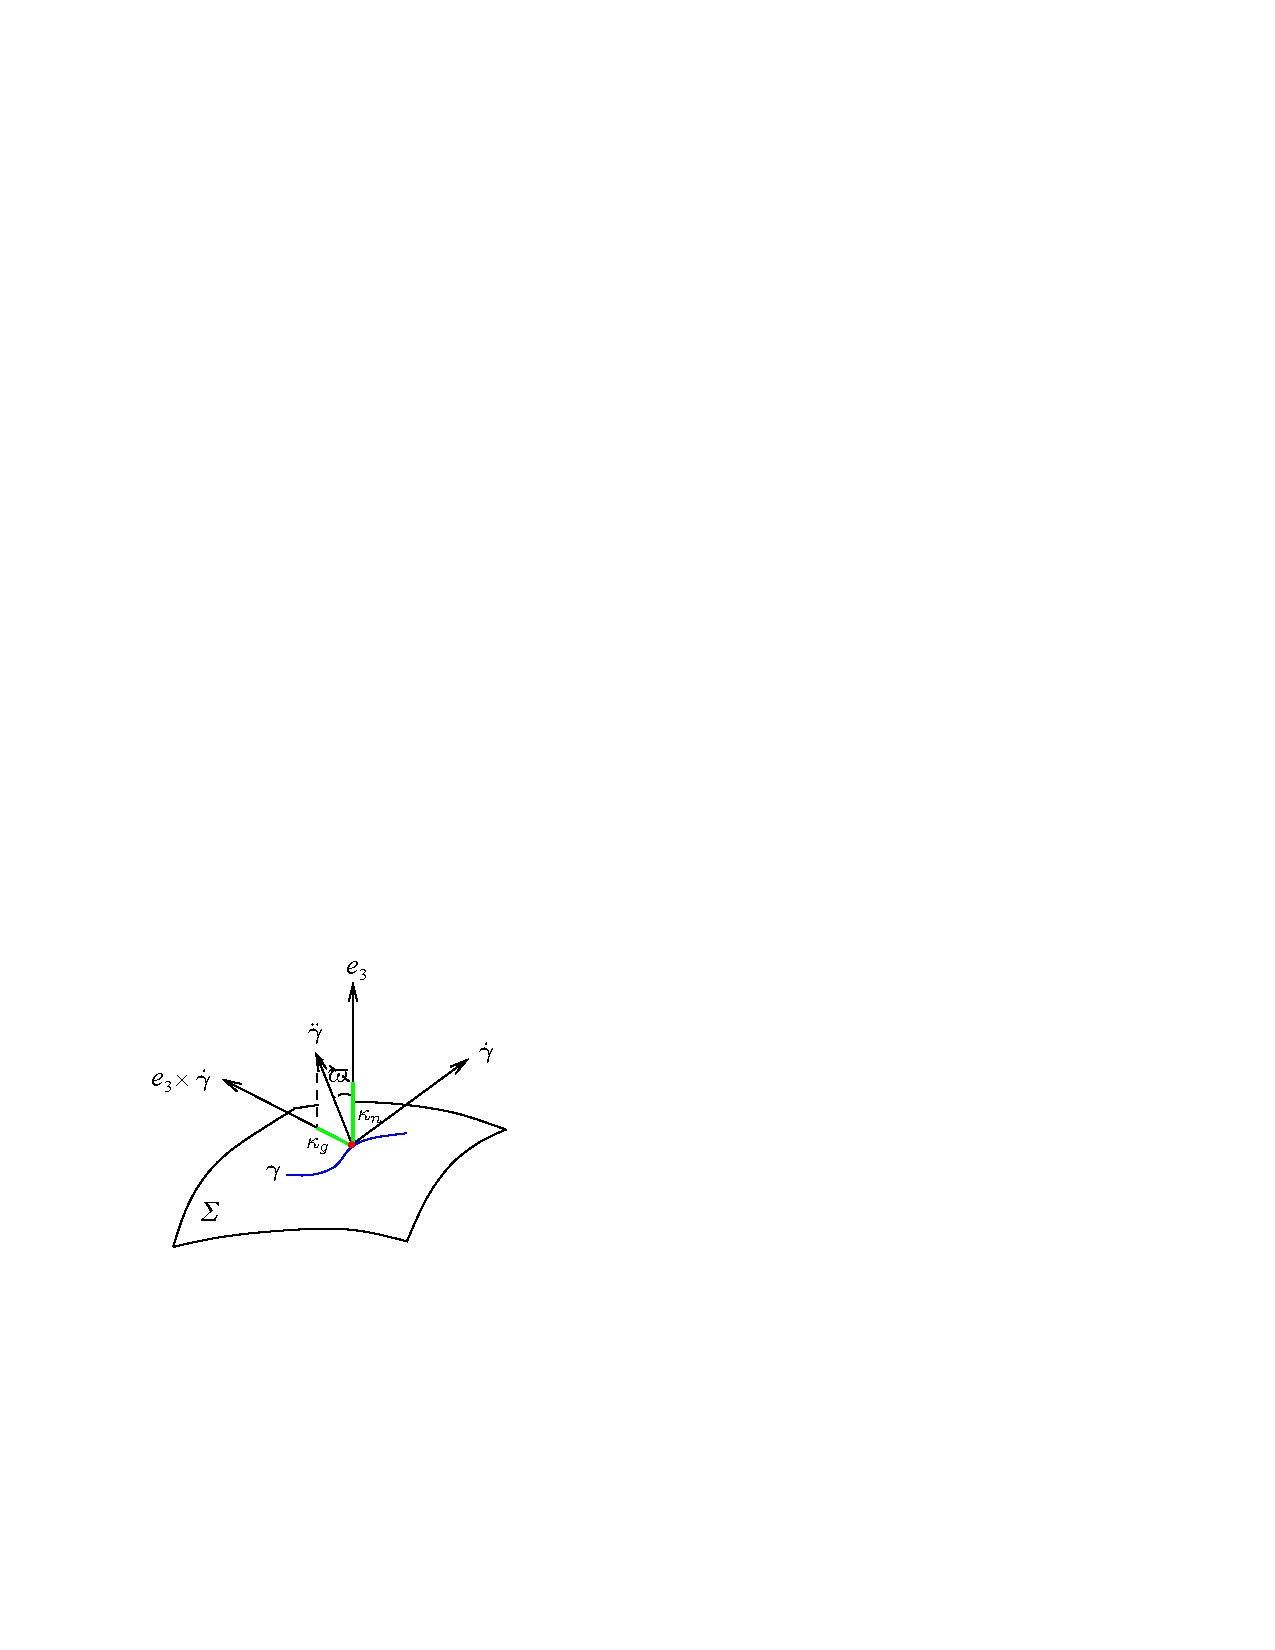
\includegraphics[scale=1]{figures/geodesic.pdf}
    \caption{Geodesic and normal curvatures of a curve on a surface.}
    \label{fig:geodesic curvature}
\end{figure}

A \emph{pseudospherical surface}\index{Pseudospherical surface} is a surface with Gauss curvature $K\equiv -1$. Setting $A=C=-1$ and $B=0$ in the \gls{eds} $\calI$ described in the last \subsect. This system is hyperbolic since $B^2-AC=-1<0$, and indeed, the $2$-forms of $\calI$ are spanned by two decomposable forms 
\[\Psi\pm \Theta=(\omega_1^3\mp \theta^2)\wedge(\omega_2^3\pm \theta^1).\]
Moreover, we may use the factors of the decomposable forms to express the second fundamental form as 
\[\rmII =\left[\frac12(\omega_1^3+\theta^2)\odot (\omega_2^3+\theta^1)-\frac12(\omega_1^3-\theta^2)\odot(\omega_2^3-\theta^1)\right]\otimes e_3,\]
where $\odot$ is the symmetric tensor product (i.e.\ $\alpha\odot \beta=\Sym(\alpha\otimes\beta)$, cf.\ \ref{def sym operator}). 
This shows that each characteristic curve projects to be an asymptotic line on $\Sigma$.

On an open subset of a pseudospherical surface that is free of umbilic points, we may choose a Darboux framing. This breaks the Cauchy characteristic symmetry of the \gls{eds}, but allows us to see how pseudospherical surfaces are connected to solutions of \gls{sge} (see Examples~\ref{ex sine-gordon} and \ref{ex 7.4.6 Ivey}).

Since we are using Darboux frames,
\[\begin{pmatrix}
    \omega^3_1\\\omega^3_2
\end{pmatrix}=\begin{pmatrix}
    \tan u & 0\\
    0 & -\cot u
\end{pmatrix}\begin{pmatrix}
    \theta^1\\\theta^2
\end{pmatrix},\]
where $u\in (0,\pi/2)$ is half of the angle between the asymptotic lines. We adjoin $u$ as a new variable, and enlarge our \gls{eds} to a Pfaffian system 
\[I=\<\theta^3,\omega^3_1-(\tan u)\theta^1,\omega^3_2+(\cot u)\theta^2\>\]
on $\SE_3\times \bbR$. Then a Darboux framing along a pseudospherical surface corresponds to an integral surface of $\calI=\<I\>_{\mathrm{diff}}$ satisfying the independence condition $\theta^1\wedge\theta^2\neq 0$, and vice versa.

The vanishing of the exterior derivatives modulo $I$ of the last two $1$-forms generating $I$ implies that $\theta^1/\cos u$ and $\theta^2/\sin u$ pull back to be closed $1$-forms on any integral surface. Hence, there exist local coordinates $(t_1,t_2)$ such that 
\[\theta^1=\cos u\dd t_1,\quad \theta^2=\sin u\dd t_2.\]
Moreover, 
\[x\coloneqq (t_1+ t_2)/2,\quad y\coloneqq (t_1-t_2)/2,\] are exactly the arclength parameters along the asymptotic lines. This implies that asymptotic lines form what is called a \emph{Chebyshev net} on the surface: parallel transport of one of the two families of curves along the other preserves it. In other words, opposite edges of the net quadrilaterals have the same length. Thus you can stretch a flexible ``knitted'' square mesh over this surface. Note also that the asymptotic lines are bisected by the lines of curvature.

Substituting $\dd u=u_x\dd x+u_y\dd y$ into the $2$-forms of the \gls{eds} shows that $\omega_2^1=u_x\dd x-u_y\dd y$ along any integral surface. Then it is easy to see that the structure equation $\dd\omega^1_2=\omega^3_1\wedge\omega^3_2$ (i.e.\ the Gauss equation) implies that $u$ (or rather $2u$) satisfies \gls{sge}:
\[u_{xy}=\sin u\cos u.\]

Conversely, we may start with a solution of the \gls{sge} and produce a pseudospherical surface by integration. On a fundamental level, note that the First and Second Fundamental Forms of a pseudospherical surface in the asymptotic coordinates $(x,y)$ read 
\[
    \rmI=\begin{pmatrix}
        1 &\cos 2u\\
        \cos 2u & 1
    \end{pmatrix},\quad
    \rmII=\begin{pmatrix}
        0 & \sin 2u\\
        \sin 2u & 0
    \end{pmatrix},
\]
and $2u$ is the angle between the $x$ and $y$-curves. From here it is easy to see that $H=-2\cot(2u)$. \gls{sge} is equivalent to the Gauss-Kodazzi equations on $H$ with $K=-1$, so by the Fundamental Theorem of Surfaces, each solution of \gls{sge} determines a unique immersed surface up to a rigid motion. 

\begin{figure}[tp]
    \centering
    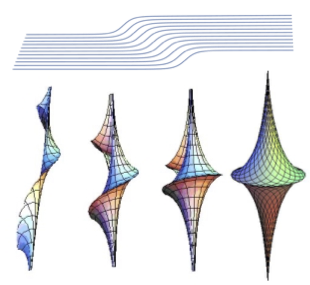
\includegraphics[scale=0.2]{figures/SG1soliton.png}
    \caption{The $1$-soliton solution (\ref{eq SGE 1-soliton}) (with lines of constant $y$) of \gls{sge} and the corresponding pseudospherical surfaces for different values of $\lambda^2$. The first three surfaces have the lines of curvature marked on them. The rightmost is the pseudosphere $\lambda=1$ with the asymptotic lines marked on it. Note the asymptotic lines becoming tangent at the edge of the surface.}
    \label{fig: SGE 1-soliton}
\end{figure}

More explicitly, if we let $\frake=(e_1,e_2,e_3)$, then the structure equations $\dd e_i=e_j\omega_i^j$ imply that 
\[\partial_x\frake=\frake \begin{pmatrix}
    0 & u_x & -\sin u\\
    -u_x & 0 & -\cos u\\
    \sin u& \cos u & 0
\end{pmatrix},\quad 
\partial_y\frake=\frake \begin{pmatrix}
    0 & -u_y & -\sin u\\
    u_y & 0 & \cos u\\
    \sin u& -\cos u & 0
\end{pmatrix}.\label{eq 7.21 Ivey}
\]
This is an overdetermined system for the matrix $\frake(x,y)$, and its Frobenius integrability condition is \gls{sge} for $u$. In fact, the above pair of equations is a $UV$-pair for \gls{sge} (see Example~\ref{ex UV pairs}; in fact, this $UV$-pair is equivalent to the one in Example~\ref{ex sine-gordon} under the isomorphism of Lie algebras $\frakso_3\cong\fraksu_2$). So, given a solution to sine-Gordon, we may obtain the framing $\frake$ by solving linear systems of ODE's, and then solve for the surface $\bf{x}(x,y)\in\bbR^3$ by integrating 
\[\bf{x}_x=e_1\cos u-e_2\sin u,\quad \bf{x}_y=e_1\cos u+e_2\sin u.\label{eq 7.22 Ivey}\]
For example, the famous \emph{1-soliton}\index{soliton} solution (also called a \emph{traveling wave} due to its translational invariance, or in the context of the sine-Gordon, a \emph{kink})
\[u=2\arctan(c\exp(\lambda x+\lambda^{-1}y)),\quad c\neq 0, \lambda\neq 0,\label{eq SGE 1-soliton}\]
gives the standard \emph{pseudosphere} when $\lambda^2=1$ and \emph{Dini's surfaces} when $\lambda^2\neq 1$, see Figure~\ref{fig: SGE 1-soliton}.\index{Pseudosphere}\index{Dini's surface} (Note that $c$ can be assumed to be $1$ after a shift and/or flip of one of the axes.)

\begin{figure}[tp]
    \centering 
    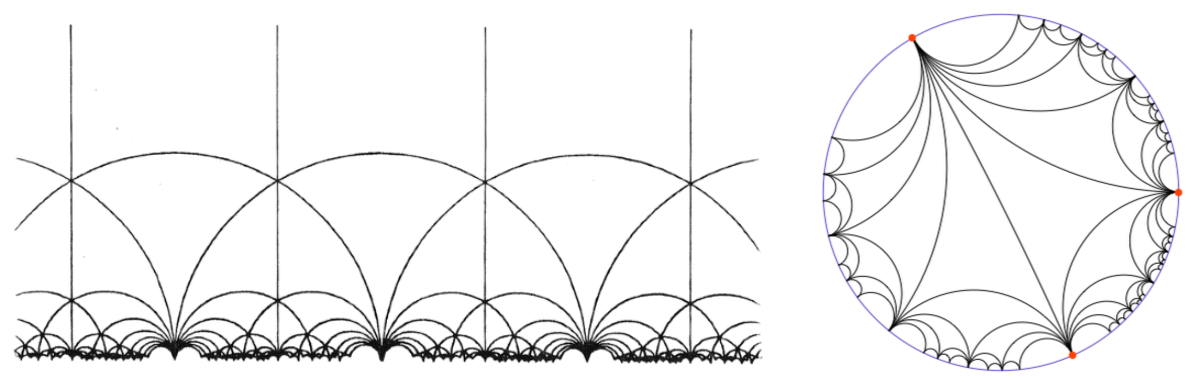
\includegraphics[scale=0.8]{figures/poincare.png}
    \caption{Poincar\'e's hyperbolic half-plane and disk models with some of their geodesics.}
    \label{fig:hyperbolic plane}
\end{figure}

\begin{example}[Hyperbolic plane and disk]
    The hyperbolic (half-)plane is the set $\bbC^+=\{z=x+\i y\in\bbC\mid \Im z>0\}$ with the Riemannian metric 
    \[\sfg=\frac{|\dd z|^2}{(\Im z)^2}=\frac{\dd x^{\otimes 2}+\dd y^{\otimes 2}}{y^2}.\]
    This metric is conformal to the Euclidean one with the conformal factor of $\lambda^2=\frac{1}{y^2}$. The Gauss curvature is found from formula (\ref{eq K in isothermal coords}): $K=\frac12y^2\partial_y^2\ln y=-1$. The geodesics of this surface are semi-circles perpendicular to the $x$-axis and vertical lines.
    
    Another hyperbolic surface of constant negative curvature is the \emph{hyperbolic disk}  $\bbD\coloneqq \{z=x+\i y\in\bbC \mid |z|<1\}$ with the metric 
    \[\sfg=\frac{4|\dd z|^2}{(1-|z|^2)^2}=\frac{4(\dd x^{\otimes 2}+\dd y^{\otimes 2})}{(1-x^2-y^2)^2}.\]
    It is easy to check that $K=-1$ again, and in fact the disk model is isometric to the half-plane one with the isometry given by the biholomorphic \emph{Cayley transform}\index{Cayley transform} 
    \[\bbC^+\to \bbD,\quad z\mapsto \frac{z-\i }{z+\i}.\]
    As a \gls{flt}, it takes circles and lines to circles and lines. As a consequence, the geodesics of the disk model are diametric lines and arcs of circles perpendicular to the bounding circle, see Figure~\ref{fig:hyperbolic plane}.
\end{example}


A Riemannian surface $(\Sigma,\sfg)$ is called \emph{(geodesically) complete} if every geodesic $\gamma(t)$ on it can be extended to all $t\in\bbR$. Equivalently, all vector fields of bounded norm are complete. The following theorem of Hilbert states that pseudospherical surfaces in Euclidean space cannot be complete. This was one of the earliest \emph{global} results in differential geometry. 

\begin{thm}[Hilbert (1901)]\index{Theorem!Hilbert}
    There is no complete immersed surface of constant negative Gauss curvature in $\bbE^3$.
\end{thm}
\begin{proof}
    Hilbert's original proof is a bit lengthy because first one has to establish that the asymptotic lines of any \emph{complete} immersed surface of constant negative curvature can be extended endlessly. Detailed expositions of this proof can be found in \cite[\S5-11]{doCarmo} and \cite[p.~251]{Spivak3}.  We will instead take an advanced shortcut by using the Uniformization Theorem (widely believed to be true since 1882 but first proved by Poincar\'e only in 1907).

    The Uniformization Theorem (in one of its formulations) states that the universal covering of any complete surface $\Sigma$ of constant negative curvature, say $K\equiv -1$, together with the pullback of the metric from $\Sigma$, is isometric to the hyperbolic plane $\bbC^+$.\footnote{This also shows that any non-compact simply connected surface (without boundary) is diffeomorphic to $\bbR^2$.} Now, if we prove that $\bbC^+$ cannot be isometrically immersed into $\bbE^3$, Hilbert's theorem will follow because the universal covering map $\pi:\bbC^+\to \Sigma$ is a local isometry, and so any isometric immersion  $\bf{x}:\Sigma\to \bbE^3$ would allow us to define an isometric immersion $\bf{x}\circ \pi:\bbC^+\to \bbE^3$ (note that we never required the immersions to be injective), leading to a contradiction.

    Now let $2u$ be the solution of \gls{sge} $(2u)_{xy}=\sin 2u$ correspoding to $\bf{x}(\bbC^+)$. Here $(x,y)$ are the asymptotic coordinates on $\bf{x}(\bbC^+)$, not to be confused with the Cartesian coordinates on $\bbC^+$. Since $\bf{x}$ is an immersion, this surface must have linearly independent asymptotic directions at each point, and hence 
    \[0<u(x,y)<\frac{\pi}{2},\quad (x,y)\in \bbC^+.\]
    Now consider a rectangle $R=[a,b]\times [c,d]\subset\bbC^+$ and compute the area of the quadrilateral $\bf{x}(R)$:
    \begin{multline}
        \mathsf{vol}\left[\restr{\bf{x}}{R}\right]=\int_R \sqrt{\det \sfg}\dd x\dd y=\int_R \sin 2 u\dd x\dd y=\int_R (2u)_{xy}\dd x\dd y=\\
        =2(u(b,d)-u(b,c)-u(a,d)+u(a,c))<2\pi.
    \end{multline}
    Since $\bbC^+$ is simply connected and $\bf{x}$ is an immersion, its asymptotic coordinates are globally defined (by stitching together local pieces if necessary), so the rectangle $R$ can be made arbitrarily large. Since the area of the hyperbolic half-plane is infinite, the area of $R$ can become arbitrarily large. This contradicts the above result showing that $\bf{x}(R)$ has bounded area, since $\bf{x}$ is supposed to be an isometry.
\end{proof}


Hence, even if the sine-Gordon solution is defined for all $x$ and $y$, the corresponding surface will become singular. In fact, $\theta^1\wedge\theta^2=\sin 2u \dd x\wedge \dd y$ shows that the surface will be singular whenever $u$ is a multiple of $\pi/2$, i.e.\ when the asymptotic lines are tangent to each other. This is why the surfaces in Figure~\ref{fig: SGE 1-soliton} have singularities and are made by joining two pseudospherical surfaces along an edge: the values of the $1$-soliton solution always span $(0,\pi)$.

\begin{rem}
    The sine-Gordon has an obvious scaling symmetry given by $x\mapsto \lambda x$, $y\mapsto \lambda^{-1}y$. Hence, each immersion of $\Sigma$ belongs to a one-parameter family of isometric immersions. These deformations of pseudospherical surfaces are called \emph{Lie transformations}. In the next \subsect\ we will find a similar one-parameter family of deformations of minimal surfaces (but parametrized by an element of $\U_1$ instead of $\bbR$ because the coresponding system is elliptic).
\end{rem}

\begin{xca}\label{xca 7.4.19 Ivey}
    Note that each of $x+y$ and $x-y$ is constant along one of the two sets of lines of curvature. 
    This observation is useful if we suppose that $\Sigma$ is a pseudospherical surface of revolution (i.e.\ is spanned by a curve when rotated about a fixed axis). Show that the corresponding sine-Gordon solution can be assumed to be of the form $u=f(x+y)$ (this is easier using the ansatz $u=2\arctan f(x+y)$). Determine all sine-Gordon solutions of this form. 
\end{xca}







\subsection{Minimal and \texorpdfstring{\gls{cmc}}{CMC} surfaces}

Recall that a minimal surface is an immersed surface $\Sigma<\bbE^3$ with vanishing mean curvature. From Proposition~\ref{prop mean curvature laplace}, an isometric immersion $\bf{x}:\Sigma\to \bbE^3$ is minimal iff it is \emph{harmonic in isothermal coordinates} $(x,y)$:
\[(\partial_x^2+\partial_y^2)\bf{x}=0.\]
In particular, $\bf{x}$ is \emph{conformal}, i.e.\ it preserves angles between tangent vectors in the $(x,y)$-plane after they're mapped to tangent vectors on $\Sigma$.

Introducing a local isothermal complex coordinate $z\coloneqq x+\i y$ (so that the metric volume form is $\sfv_\sfg=\lambda^2\dd x\wedge\dd y=\lambda^2\frac{\i}{2}\dd z\wedge\dd\wb{z}$), this suggests that there exist $3$ (locally) holomorphic functions of $z$ whose real parts are exactly the Cartesian components of $\bf{x}$. We seek to find this representation now.

Setting $A=C=0$ and $B=1$ in the \gls{eds} for a general linear Weingarten equation shows that the $2$-forms of $\calI$ are spanned 
\[\Theta=-\dd\theta^3,\quad \Psi=\omega^3_2\wedge\theta^1-\omega^3_1\wedge\theta^2.\]
This system is elliptic since $B^2-AC=1>0$, so we will have to adjust our method of characteristics to solve it. We will see below that studying the characteristic systems of $\calI$ leads to the classical \emph{Weierstrass representation} for minimal surfaces, which relates them to complex Riemann surfaces.

When we attempt to form the characteristic systems, we find that the decomposability equation 
\[(\Theta+\lambda\Psi)^{\wedge 2}=0\]
has constant roots $\lambda=\pm\i$. So, we need to introduce complex-valued differential forms. For example,
\[\Theta\pm \i \Psi=(\omega^3_1\mp \i \omega^3_2)\wedge(\theta^1\pm\i \theta^2),\]
and so if we define 
\[\omega\coloneqq \omega^3_1-\i \omega^3_2,\quad \theta\coloneqq \theta^1+\i \theta^2,\]
then the characteristic systems are 
\[\calM=\<\theta^3,\omega,\theta\>,\quad \wb\calM=\<\theta^3,\wb\omega,\wb\theta\>.\]

When we attempt to apply Darboux's method, we find that neither of these systems contains a rank-$2$ integrable subsystem. In fact, $\dd\omega\equiv 0\pmod{\omega}$, but $\dd\theta\equiv \wb\omega\wedge\theta^3\pmod{\theta}$. However, this shows that the distribution
\[\Re\<\omega,\wb\omega\>=\<\omega^3_1,\omega^3_2\>\eqqcolon J\]
is a Frobenius system on $\SE_3$. The quotient of $\SE_3$ by the leaves of the distribution dual to $J$ is a $2$-sphere, and the quotient map $\gamma:\SE_3\to \bbS^2$ is given by the unit vector $e_3$. Thus, the restriction of $\gamma$ to an integral surface $M$ of $\calI$ is just the Gauss map of the minimal surface $\Sigma=\pi(M)$, where $\pi:\SE_3\to \bbE^3$ is the bundle projection.

Since $\omega$ descends, via $\gamma$, to a well-defined (up to multiple) form on $\bbS^2$, we can define a complex structure on the sphere for which $\omega$ spans the \emph{$(1,0)$-forms}, i.e.\ the subbundle of $T^\ast \bbS^2$ locally spanned by $\dd w$ for a local complex coordinate $w$. We have shown the following fundamental fact.

\begin{cor}
    The Gauss map of a minimal surface $\Sigma$ is holomorphic with respect to the complex structure on $\Sigma$ defined by $\theta=\theta^1+\i \theta^2$ (as a $(1,0)$-form).
\end{cor}

Now let us fix a standard complex coordinate on $\bbS^2$. We identify $\bbS^2$ with the null quadric $N\subset \CP^2$ defined by $z_1^2+z_2^2+z_3^2=0$ on $\bbC^3$, by mapping $e_3$ to the vector 
\[\mathsf{z}\coloneqq e_1-\i e_2 \quad \in\bbC^3\cong \bbR^3\otimes\bbC.\]
In fact, this vector can be determined from $e_3$ in a unique way, up to a scale, by the requirement that $e_3\times \mathsf{z}=\i \mathsf{z}$. Note that the equation defining $N$ implies that $\lVert\Re \mathsf{z}\rVert^2=\lVert\Im \mathsf{z}\rVert^2=\frac12\lVert \mathsf{z}\rVert^2$.

We then use the stereographic projection 
\[\mathsf{z}=\begin{pmatrix}
    1-w^2\\ \i(1+w^2)\\ 2w
\end{pmatrix},\quad w\in\bbC,\]
to define a complex local coordinate $w$ on $N$ (this actually agrees with the standard stereographic projection $\bbC\to \CP^1\setminus\{\infty\}$ given by $w\mapsto \frac{1}{1+|w|^2}(2w,1-|w|^2)=(x^1+\i x^2,x^3)$, so the resulting complex structure induced by $\omega$ on $\bbS^2$ is the standard one). Computing $\dd\mathsf{z}$ and comparing with $\dd(e_1-\i e_2)=\i(e_1-\i e_2)\omega^1_2+e_3\omega$ shows that $\gamma^\ast\dd w$ is a multiple of $\omega$.

Now suppose $z$ is a complex coordinate on our minimal surface $\Sigma$. Then $\theta=f(z)\dd z$ for a nonvanishing holomorphic function $f$, and $\gamma^\ast w=g(z)$ for some holomorphic function $g$ (we can think of $g(z)$ as another local complex coordinate). Notice that the point $\bf{x}\in \Sigma$ satisfies 
\[\dd \bf{x}=e_1\theta^1+e_2\theta^2=\Re((e_1-\i e_2)(\theta^1+\i \theta^2))=\Re(\mathsf{z}\theta).\]
As a consequence, the First Fundamental Form $\rmI=\<\dd\bf{x},\dd\bf{x}\>$ reads 
\[\rmI=\frac12\lVert\mathsf{z}\rVert^2 |\theta|^2=\frac14 \left(1+|g|^2\right)^2 |f|^2 |\dd z|^2,\quad |\theta|^2\coloneqq \theta\odot\wb\theta.\]
Thus, $z$ is an isothermal coordinate. Similarly, the Second Fundamental Form is 
\[\rmII=-\<\dd e_3,\dd\bf{x}\>e_3=-\Re(\theta \otimes \dd g)e_3.\]
(This is automatically symmetric because $\theta\wedge\dd g\propto \dd z\wedge\dd z=0$.)
In particular, a vector $X$ is an asymptotic direction iff $\theta(X)\dd g(X)$ is imaginary, and principal iff it is real. The Gauss curvature is easy to compute from the conformal factor since the metric is already diagonalized (here we're using informal notation for dividing tensors; the trickiest part is the sign):
\[K=-\frac{|\theta|^2|\dd g|^2}{\left(\frac12\Vert \mathsf{z}\rVert^2 |\theta|^2\right)^2}=-\left(\frac{4|g'|}{(1+|g|^2)^2|f|}\right)^2.\]

Finally, by substituting the expressions for $\mathsf{z}$ and $\theta$ in terms of $z$, we find the \emph{Weierstrass-Enneper representation} of $\Sigma$:
\[\bf{x}=\Re\int \mathsf{z}\theta=\Re\int 
\begin{pmatrix}
    (1-g^2)f\\ \i (1+g^2)f\\ 2gf
\end{pmatrix}\dd z.\label{eq Weiestrass-Enneper}\]
Here, the integral is a contour integral of a holomorphic $1$-form, taken from an arbitrary basepoint to the given point, and is independent of homotopic deformations of the contour with fixed endpoints. Hence, it produces a well-defined function of the endpoint. 

Note that, generally, $g$ is allowed to be a meromorphic function on a domain with nontrivial topology ($\gamma$ takes values in $\bbS^2=\CP^1$, and thus can have poles), which allows $\Sigma$ to have nontrivial topology as well. Moreover, it is obvious from the formulas that the Weierstrass parametrization is regular as long as the poles of $g$ coincide with (and are at most half of the order of) the zeros of $f$.

\begin{cor}[Weiestrass-Enneper representation]\index{Weierstrass-Enneper representation}
    Each nonplanar minimal surface $\Sigma<\bbE^3$ is determined, up to rigid motions, by its Weierstrass data consisting of a meromorphic function $g:\Sigma\to \CP^1$ and a $1$-form $\theta\in\Omega^1(\Sigma;\bbC)$ that is holomorphic with respect to the complex structure on $\Sigma$ induced by the metric and orientation. Conversely, every such pair $(g,\theta)$ determines a minimal surface via (\ref{eq Weiestrass-Enneper}) as long as the poles of $g$ overlap with zeros of $\theta$ so that $g^2\theta$ is holomorphic.
\end{cor}

We can immediately observe that multiplying $f$ (or $\theta$) by a unit complex number produces another valid minimal immersion of the same metric surface.

\begin{defn}[Associate family, conjugate surface]\index{Associate family}\index{Conjugate surface}
    Given a minimal surface $\bf{x}:\Sigma\to \bbE^3$ with Weierstrass-Enneper representation $(g,\theta)$, the one-parameter family of isometric minimal surfaces corresponding to $(g,\rme^{\i t}\theta)$, $t\in (0,2\pi)$, is called the associate family of minimal surfaces.
    
    In particular, the conjugate surface to $\Sigma$ is the surface obtained by multiplying $\theta$ by $\rmi$, or equivalently, by replacing $\Re$ with $\Im$ in (\ref{eq Weiestrass-Enneper}).
\end{defn}

\begin{example}[Catenoid and helicoid]
    The Weierstrass-Enneper representation for the catenoid as parametrized in Example~\ref{ex catenoid} (coordinates $(u,v)$ there are, in fact, isothermal) is 
    \[f(z)=-\i \rme^{-\i z/a},\quad g(z)=\rme^{\i z/a},\quad a>0,\]
    and its conjugate surface is the helicoid (although a slight reparametrization will be necessary to bring to the same form as in Example~\ref{ex helicoid}). This agrees with the standard way of picturing the Riemann surface of $z=\ln w$ as a helicoid. The rest of this $1$-parameter family of surfaces is shown in Figure~\ref{fig:helicoid}.
\end{example}


\begin{xca}
    \begin{enumerate}
        \item Identify the surfaces corresponding to $f=1$ and $g$ being one of $0,z,z^{-1},\i z^{-1}$. The surface with $g(z)=z$ is called the \emph{Enneper surface}\index{Enneper surface} and is the only member of its associate family (in particular, conjugate to itself).
        \item Conclude that the surface obtained by using $(f,g)=(\cos^2\frac{z}{2},\tan\frac{z}{2})$ is regular, and identify it with one of the surfaces in item 1. This shows that the Weierstrass representation of a given minimal surface is not unique.
    \end{enumerate}
\end{xca}

Now let us expand the scope to include \gls{cmc} surfaces. Setting $A=0$, $B=1$, and $C=-2H$, with $H$ a given constant, we get a Weingarten \gls{eds} with $2$-forms 
\[\Theta=-\dd\theta^3,\quad \Psi=\omega^3_1\wedge\theta^2+\theta^1\wedge\omega^3_2-2H\theta^1\wedge\theta^2.\]
As with the minimal surface system, the characteristics are complex. The decomposable $2$-forms are 
\[\Theta+ \i \Psi=(\omega-H\wb\theta)\wedge\theta\]
and its complex conjugate. This complex coframe, adapted as it is to the characteristics, leads to a simple basis for the \gls{eds} and a simple description of its prolongation. Namely, we adjoin a complex variable $q$ and define the $1$-form 
\[\tau\coloneqq \omega-H\wb\theta-q\theta.\]
The prolongation is the Pfaffian system $\<\theta^3,\tau,\wb\tau\>$ on $\SE_3\times\bbC$. The system $2$-forms are 
\[\dd\tau\equiv -(\dd q+2iq\omega^1_2)\wedge\theta\pmod{\theta^3,\tau,\wb\tau}\]
and its complex conjugate. Note that $q$ parametrizes the components of the traceless part of the Second Fundamental Form. For, $\tau=0$ implies that 
\[\begin{pmatrix}
    \omega^3_1\\\omega^3_2
\end{pmatrix}=\begin{pmatrix}
    H+q_1 & -q_2\\
    -q_2 & H-q_1
\end{pmatrix}\begin{pmatrix}
    \theta^1\\\theta^2
\end{pmatrix},\]
where $q=q_1+\i q_2$. Thus, the zeros of $q$ are the umbilic points of the surface.

\begin{prop}[{{\cite[Prop.~7.4.25]{Ivey}}}]\label{prop 7.4.25 Ivey}
    Let $\Sigma$ be an oriented surface with a Riemannian metric, and let $P$ be its oriented orthonormal frame bundle, with the canonical forms $\eta^1,\eta^2$ and connection form $\eta^1_2$ (see Remark~\ref{rem covariant derivative on surfaces}). Endow $\Sigma$ with the complex structure which it inherits from the metric and orientation. Suppose $q$ is a complex-valued function on $P$ that satisfies 
    \[(\dd q+2\i q\eta^1_2)\wedge(\eta^1+\i \eta^2)=0.\label{eq 7.28 Ivey}\]
    Then 
    \begin{enumerate}
        \item then
        \[Q\coloneqq q(\eta^1+\i \eta^2)^{\otimes 2}\]
        is a well-defined holomorphic quadratic differential on $\Sigma$.
        \item For any constant $H$, $q$ determines a unique local isometric embedding of $\Sigma$ as a \gls{cmc} surface of mean curvature $H$ into $\bbE^3$ up to rigid motions.
        \item An immersed surface is \gls{cmc} iff its Hopf differential (the traceless part of the $\wt{Q}$ defined in \Subsect~\ref{sec: theory of surfaces}) is holomorphic.
    \end{enumerate}
\end{prop}
\begin{proof}
    To see that the differential $Q$ is well-defined, let $X$ be the vector field tangent to the fibers of $P$ that is dual to $\eta^1_2$. Then it is easy to check that $\Lie_X Q=0$. To see that it is holomorphic, let $Q=p\dd z^{\otimes 2}$, where $z$ is a local complex coordinate such that $\dd z$ is a multiple of $\eta^1+\i \eta^2$. Then (\ref{eq 7.28 Ivey}) implies that $\partial_{\wb z}p=0$.

    Any isometric immersion of $\Sigma$ into $\bbE^3$ will induce an immersion from $P$ to $\SE_3$, and the graph of this map will be an integral $3$-manifold of the Pfaffian system on $P\times \SE_3$ generated by 
    \[\<\theta^3,\theta^1-\eta^1,\theta^2-\eta^2,\omega^1_2-\eta^1_2\>.\]
    To this system we adjoin the form $\tau$ and its conjugate, where $q$ is now given. Our hypothesis about $q$ implies that this enlarged system is Frobenius. Thus, there exists a unique integral $3$-manifold through each point, and any two isometric immersions differ by a rigid motion.
\end{proof}

\begin{cor}[Hopf]\index{Theorem!Hopf}
    Any \gls{cmc} immersion of a sphere $\Sigma=\bbS^2$ (with any metric) is a round sphere, i.e.~$K\equiv H^2=\const$.
\end{cor}
\begin{proof}
    It suffices to show that the space of holomorphic quadratic differentials on a sphere is trivial.
    Choose the standard complex structure on the sphere $\CP^1=\bbC\cup \{\infty\}$ given by the complex coordinate $z\in\bbC$. Any \gls{cmc} immersion corresponds to a holomorphic differential $Q=q\dd z^{\otimes 2}$ on $\CP^1$. Then $q$ is a function holomorphic in $\bbC$, and moreover $Q$ needs to be holomrphic at $\infty$, which means that in the local coordinate $w=z^{-1}$, the expression $Q=q(z)w^{-4}\dd w^{\otimes 2}=q(z)z^{4}\dd w^{\otimes 2}$ has to remain regular as $z\to \infty$. Thus $q(z)z^4\to 0$ as $z\to\infty$. But the only holomorphic function in $\bbC$ that has this property is zero, thus $Q=0$ and $K=H^2$.
\end{proof}


\begin{cor}[Bonnet {{\cite[Cor.~7.4.26]{Ivey}}}]
    Any \gls{cmc} surface has a circle's worth of isometric deformations as a \gls{cmc} surface.
\end{cor}
\begin{proof}
    Given $f:\Sigma\to \bbR^3$, let $q$ be the coefficient of the Hopf differential as above and let 
    \[q^t\coloneqq \rme^{\i t}q,\quad t\in(0,2\pi).\label{eq 7.29 Ivey}\]
    Then $q^t$ also satisfies the conditions of Proposition~\ref{prop 7.4.25 Ivey}, and the First Fundamental Form remains unchanged.
\end{proof}

Moreover, if the surface is not totally umbilic, then at most points $q\neq 0$ and the Second Fundamental Form is changed by (\ref{eq 7.29 Ivey}). So, the surface constructed using $q^t$ is, in general, not congruent to the original surface by rigid motions. This is the \gls{cmc} generalization of the isometric deformations of minimal surfaces that we saw above.

\begin{rem}[Bonnet surfaces]
    The above deformations show that there are noncongruent surfaces with the same $K$ and $H$ (in this case, $H$ is the same constant). Bonnet discovered that, besides \gls{cmc} surfaces, there is a finite-dimensional family of surfaces that admit noncongruent isometric deformations preserving $H$. These \emph{Bonnet surfaces} may be characterized by the property that they admit isothermal coordinates (so $q$ is real) and in these coordinates $1/q$ is harmonic, i.e.\ $(1/q)_{z\wb z}=0$.
\end{rem}










\subsection{B\"acklund transformations}


Equations which are integrable by the method of Darboux give one example where we can construct integral manifolds of an \gls{eds} by restricting to a submanifold where the system becomes Frobenius. Another example arises when the integrability condition for an overdetermined system of PDE's can be reduced to finding the solution of another PDE. Then any solution of that PDE enables us to construct (using ODE techniques) a solution of the original system.

\begin{example}\label{ex 7.5.1 Ivey}
    For example, the $UV$-pair representation (\ref{eq 7.21 Ivey}) of \gls{sge} enables us to construct a solution to the \gls{ma} system for pseudospherical surfaces by integrating a Frobenius system.
\end{example}

When this transformation works in both directions, the two PDE's are said to be related by a \emph{B\"acklund transformation}, which we will define later in the section. First, we formalize the relationship between the systems seen in the above examples.

\begin{defn}
    Let $\calI$ be an \gls{eds} on a manifold $M$, let $\pi:B\to M$ be a submersion, and let $\calE$ be an \gls{eds} on $B$. Then $\calE$ is an integrable extension of $\calI$ if there exists a Pfaffian system $J<T^\ast B$ such that 
    \[\calE=\<J\cup \pi^\ast\calI\>_{\mathrm{alg}}\label{eq 7.31 Ivey}\]
    and $J$ is transverse to the fibers of $\pi$ (i.e. a frame of $J$ pulls back to form coframes on each fiber of $\pi$).  The \emph{rank} of an integrable extension is the rank of $J$, or the dimension of the fibers of $\pi$.
\end{defn}


The condition that $\calE$, as defined by (\ref{eq 7.31 Ivey}), is a differential ideal is equivalent to 
\[\dd\theta\equiv 0\pmod{J,\pi^\ast\calI}\text{ for any }\theta\in\Gamma^\infty(J).\label{eq 7.32 Ivey}\]


\begin{example}[Laplace equation]\index{Equation!Laplace}\label{ex laplace equation backlund}
    The ``baby version'' of a B\"acklund transformation is the Cauchy-Riemann system, which relates pairs of solutions to the $2$-dimensional Laplace equation. Recall from Example~\ref{ex 7.4.6 Ivey} that the Laplace equation $u_{xx}+u_{yy}=0$ is equivalent to the \gls{ma} system on $J^1(\bbR^2,\bbR)$ generated (differentially) by $\theta=\dd z-p \dd x-q \dd y$ and $\Psi=\dd p\wedge\dd y-\dd q\wedge \dd x$. We observe that 
    \[\Psi=\dd (p\dd y-q \dd x)\eqqcolon \dd \phi,\]
    so we can extend the system to $J^1(\bbR^2,\bbR)\times\bbR$ with a new variable $w$ and let the Pfaffian system $J$ be 
    \[J=\<\dd w-\phi\>=\<\dd w+q\dd x-p\dd y\>.\]
    Clearly $J$ satisfies (\ref{eq 7.32 Ivey}) because $\dd (f\phi)\equiv 0\pmod{\<\phi,\Psi\>}$. Meanwhile, the extended system $\calE$ is a Pfaffian system spanned by $\theta$ and $\phi$, which is equivalent to the following pair of equations on two functions $z=u(x,y)$ and $w=v(x,y)$:
    \[u_x=v_y,\quad u_y=-v_x,\]
    i.e.\ the Cauchy-Riemann system.\index{Equation!Cauchy-Riemann} Whenever $u,v$ satisfy this system, both $u$ and $v$ must be harmonic. The Cauchy-Riemann system allows one to easily compute $v$ from $u$ (up to constants of integration) using ODE methods. Hence, this system can be seen as a method for generating ``new'' harmonic functions from known ones. Such pairs of harmonic functions are called \emph{conjugate}.\index{Conjugate harmonic function}
\end{example}

If $(B,\calE)$ is an integrable extension of rank $k$ and $N\subset M$ is a $p$-dimensional integral manifold of $\calI$, then (\ref{eq 7.32 Ivey}) implies that the pullback of $J$ to $\pi^{-1}(N)$ is Frobenius. In this way, an integral manifold of $\calI$ gives a $k$-parameter family of integral manifolds of $\calE$. In Example~\ref{ex 7.5.1 Ivey}, the $6$-parameter family of surfaces corresponding to a single sine-Gordon solution are congruent under rigid motions of $\bbE^3$.


\begin{example}[\ref{ex 7.5.1 Ivey} continued]
    Let $M=\bbR^5$ and let $\calI$ be the \gls{ma} system for \gls{sge} given in Example~\ref{ex 7.4.6 Ivey}. Let $B=M\times \SE_3$. The equations (\ref{eq 7.21 Ivey}) and (\ref{eq 7.22 Ivey}) show that a Darboux framing for a pseudospherical surface associated to a sine-Gordon solution $u(x,y)$ is an integral surface for the Pfaffian system 
    \begin{multline}
        J\coloneqq \<\theta^1-\cos u(\dd x+\dd y),\theta^2+\sin u(\dd x-\dd y),\omega^1_2-u_x \dd x+u_y\dd y,\right.\\
        \left. {}\omega^3_1-\sin u(\dd x+\dd y),\omega^3_2+\cos u(\dd x-\dd y)\vphantom{|}\>.
    \end{multline}
    The one can check that $J$ satisfies (\ref{eq 7.32 Ivey}).
\end{example}


\begin{rem}\label{rem 7.5.4 Ivey}
    Suppose $\calI$ is a \gls{eds} on a manifold $M$ with a $2$-form $\Phi\in\calI^2$ closed. Then, by the Poincar\'e Lemma~\ref{lem poincare classic}, in some contractible neighborhood of any given point in $M$ there exists a differential form $\phi$ such that $\dd\phi=\Phi$. We may define a rank-$1$ integrable extension of $\calI$ by introducing a new coordinate $y$ and letting the Pfaffian system $J$ on $U\times\bbR$ be spanned by $\dd y-\phi$. This is exactly what we did for the Laplace equation in Example~\ref{ex laplace equation backlund}. Because such forms $\Phi$ are examples of conservations laws for an \gls{eds}, we call this construction an \emph{extension via conservation law}.
\end{rem}


\begin{rem}
    One could trivially produce an integrable extension by choosing $J$ to be Frobenius. Such extensions are called \emph{flat}. More generally, if the derived flag of $J$ terminates in a Frobenius system $K$ of rank $k'$, then $\calE$ defines an intgerable extension when pulled back to any leaf of the foliation dual to $K$. In this case $(B,\calE)$ is called a \emph{$k'$-parameter family} of integrable extensions.
\end{rem}

Parametric families of integrable extensions are frequently encountered in the study of completely integrable PDE's, i.e.\ \emph{solitonic equations}. 

\begin{example}\label{ex 7.5.6 Ivey}
    We now describe the integrable extensions of the \gls{kdv} equation 
    \[u_t+u_{xxx}+6uu_x=0\label{eq 7.33 Ivey}\]
    (it coincides with (\ref{eq kdv})) after flipping the sign of $u$). Let $M=\bbR^5$ with coordinates $(x,t,u,p,r)$. Let 
    \begin{align}
        \Theta_1\coloneqq &(\dd u-p\dd x)\wedge\dd t,\\
        \Theta_2\coloneqq &(\dd p-r\dd x)\wedge\dd t,\\
        \Theta_3\coloneqq &(\dd r+6u p\dd x)\wedge \dd t-\dd u\wedge\dd x,
    \end{align}
    and let $\calI=\<\Theta_1,\Theta_2,\Theta_3\>_{\mathrm{diff}}$. Then solutions of (\ref{eq 7.33 Ivey}) correspond to integral surfaces of $\calI$ satisfying the independence condition $\dd x\wedge\dd t\neq 0$. (Note that $M$ is a quotient of $J^2(\bbR^2,\bbR)$, and $p,r$ have their classical meanings as $u_x$ and $u_{xx}$ respectively. One could also use the \gls{eds} obtained by pulling back the standard contact system on $J^3(\bbR^2,\bbR)$ to the hypersurface defined by (\ref{eq 7.33 Ivey}), but the extra variables are not needed here.)

    On $B=M\times\bbR^2$ with fiber coordinates $(\mu,y)$, let $J=\<\dd \mu,\eta\>$, where 
    \[\eta\coloneqq \dd y-(y^2+u-\mu)\dd x+(r+2py+2(u+2\mu)(y^2+u-\mu))\dd t,\]
    and let $\calE=\<J\cup \calI\>_{\mathrm{alg}}$. It is an exercise to verify that $\calE$ is an integrable extension of $\calI$.

    Since $J$ contains a rank-$1$ Frobenius system, we have a $1$-parameter family of extensions, with $\mu$ as a parameter. Along an integral surface of $\calE$ that satisfies the independence condition, $y(x,t)$ satisfies 
    \[y_y+y_{xxx}+6(\mu-y^2)y_x=0\label{eq 7.34 Ivey}\]
    for some constant $\mu$. This family of equations may be said to be extensions of \gls{kdv}. When $\mu=0$, it is a version of another well-known PDE, the \emph{modified \gls{kdv} equation}, and the passage from $u$ to $y$ is known as the \emph{Miura transformation}.
    % All integrable extensions of \gls{kdv} have been classified, and each of them corresponds to a finite-dimensional representation of a certain infinite-dimensional Lie algebra, known as the \emph{\gls{kdv} prolongation algebra}. Moreover, this algebra has a $1$-parameter family of finite-dimensional quotients, each of which is isomorphic to a semidirect product of $\fraksl_2(\bbR)$ with $\bbR^5$. Representations of the latter algebra allow us to construct $1$-parameter families of \gls{kdv} extensions, the most well-known of which is the AKNS system (\ref{eq AKNS UV pair})
\end{example}


B\"acklund transformations are a particular form of integrable extension which allows a two-way transformation of solutions of a PDE to solutions of another (or the same) PDE. One of the most well-known is the following transformation, which can produce new solutions of the \gls{sge}.

\begin{example}\label{ex 7.5.9 Ivey}
    Consider the system
    \begin{align}
        u_x-\wb{u}_x=\lambda&\sin(u+\wb{u}),\\
        u_y+\wb{u}_y=\frac{1}{\lambda}&\sin(u-\wb{u}).
    \end{align}
    If $u(x,y),\wb{u}(x,y)$ are smooth functions that satisfy this system for some $\lambda\neq 0$, the differentiating and equating mixed partials implies that $u$ and $\wb{u}$ must be solutions of sine-Gordon $u_{xy}=\sin u\cos u$. Conversely, given a solution $u(x,y)$ of sine-Gordon, we can determine $\wb{u}_x$ and $\wb{u}_y$ from the above, and integrate to get the new solution $\wb{u}(x,y)$ (since we are guaranteed that mixed partials commute). Since this can be done for any $\lambda$, and there will be a constant of integration of the first-order ODE, we get a $2$-parameter family of solutions. For example, the kink solution (\ref{eq SGE 1-soliton}) can be produced in this way by starting with $u\equiv 0$. However, the constants of integration amount to translating the solution in the plane, so we can omit them, keeping the translational invariance in mind. Thus, the kink has one parameter $\lambda$. By iterating this procedure, we get a $2$-parameter family of $2$-soliton solutions, a $3$-parameter family of $3$-soliton solutions, and so on. All of them can be obtained by solving simple ODE's and are expressed in terms of trigonometric and exponential functions. For example, the $2$-soliton solution (Figure~\ref{fig:2-soliton}) is 
    \[u=2\arctan \frac{\lambda_1+\lambda_2}{\lambda_1-\lambda_2}\frac{\rme^{\lambda_1x+\lambda_1^{-1}y}-\rme^{\lambda_2 x+\lambda_2^{-1}y}}{1+\rme^{(\lambda_1+\lambda_2)x+(\lambda_1^{-1}+\lambda_2^{-1})y}}.\label{eq sge 2-soliton}\]
    One can also obtain other interesting exact solutions from these formulas. While $\lambda_1$ and $\lambda_2$ are real, we can put $\lambda_1=\rme^{\i t}=-\lambda_2^{-1}$ for $t\in \bbR$, and discover that the formula for the $2$-soliton solution gives another real solution of sine-Gordon, which is periodic in $x-y$ and is called a \emph{breather} (Figure~\ref{fig:breather}).
\end{example}

\begin{figure}[tp]
    \centering
    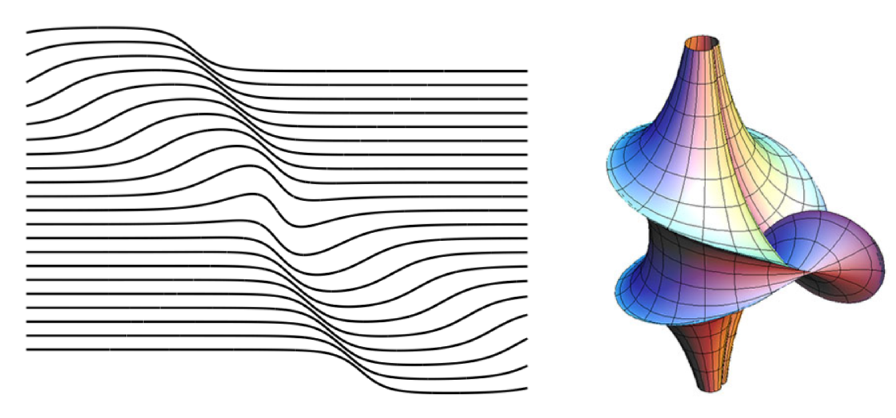
\includegraphics[scale=0.2]{figures/SG2soliton.png}
    \caption{A $2$-soliton solution of \gls{sge} (height profiles at constant $y$ for (\ref{eq sge 2-soliton})) and the corresponding pseudospherical surface.}
    \label{fig:2-soliton}
\end{figure}


\begin{defn}[B\"acklund transformation]
    Let $M_1,M_2$ carry \glspl{eds} $\calI_1$ and $\calI_2$, respectively, and let $B\subset M_1\times M_2$ be a submanifold such that the projections $\pr_i:B\to M_i$, $i=1,2$, give $B$ the structure of a double fiber bundle. Then $(B,\calE)$ defines a B\"acklund transformation between $\calI_1$ and $\calI_2$ if $\calE$ is an \gls{eds} on $B$ that is an integrable extension of both $\calI_1$ and $\calI_2$.
\end{defn}

We will often define B\"acklund transformations by giving a Pfaffian system $J<T^\ast B$ such that 
\begin{align}
    &\<J\cup \pr_1^\ast \calI_1\>_{\mathrm{alg}}=\<J\cup \pr_2^\ast\calI_2\>_{\mathrm{alg}},\label{eq 7.37a Ivey}\\
    &\calE\coloneqq \<J\cup \pr_1^\ast \calI_1\cup \pr_2^\ast \calI_2\>_{\mathrm{alg}}\text{ is a differential ideal}.\label{eq 7.37b Ivey}
\end{align}
Note that $J$ need not be transverse to the fibers of $\pr_1$ or $\pr_2$.

\begin{example}[\ref{ex 7.5.9 Ivey} continued]
    Let $M_1$ and $M_2$ be two copies of $J^1(\bbR^2,\bbR)$ where we denote the forms and coordinates on $M_2$ with bars. For $i=1,2$ let the \gls{eds} $\calI_i$ on $M_i$ be a copy of the \gls{ma} system for \gls{sge} from Example~\ref{ex 7.4.6 Ivey}. For any $\lambda\neq 0$, let $B_\lambda<M_1\times M_2$ be defined by $\wb{x}=x$, $\wb{y}=y$ and 
    \begin{align}
        p-\wb{p}=&\lambda\sin(u+\wb{u}),\\
        q+\wb{q}=&\frac{1}{\lambda}\sin(u-\wb{u}).
    \end{align}
    Let $\theta$ be the standard cotact form on $J^1(\bbR^2,\bbR)$. On $B_\lambda$, let $J=\<\pr_1^\ast\theta,\pr_2^\ast\wb\theta\>$. Then it is easy to check that (\ref{eq 7.37a Ivey}-\ref{eq 7.37b Ivey}) are satisfied.
\end{example}

\begin{figure}[tp]
    \centering
    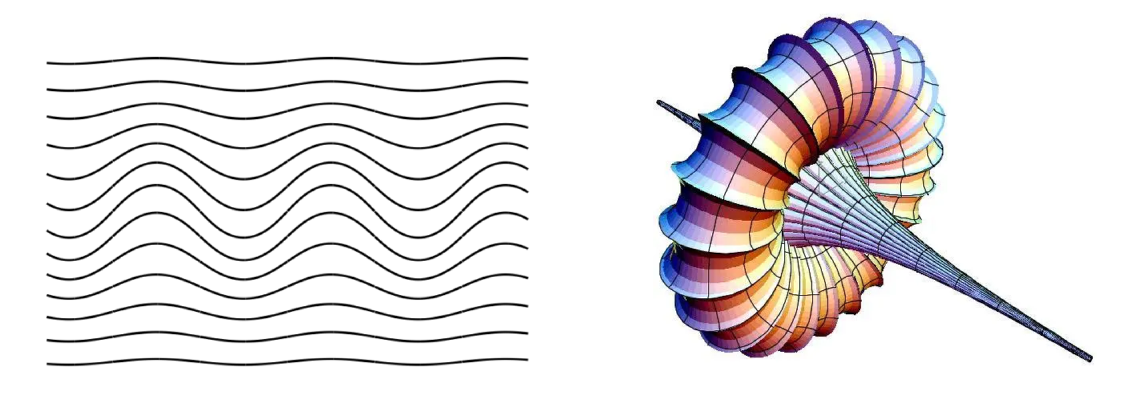
\includegraphics[scale=0.2]{figures/SGbreather.png}
    \caption{A breather wave solution of \gls{sge} (height profiles at constant $x+y$) and the corresponding pseudospherical surface.}
    \label{fig:breather}
\end{figure}


\begin{example}[\ref{ex 7.5.6 Ivey} continued]
    Let $M_1,M_2$ be two copies of $\bbR^5$, each carrying a copy of the \gls{kdv} \gls{eds}. (Again, we use barred coordinates on $M_2$.) Define $B=M_1\times\bbR^2$ as before, and define a submersion $\pr_2:B\to M_2$ by 
    \begin{align}
        \wb{x}&=x,\\
        \wb{y}&=y,\\
        \wb{u}&=2(\mu-y^2)-u,\\
        \wb{p}&=4y(\mu-u-y^2)-p,\\
        \wb{r}&=-4(u+y^2-\mu)(u+3y^2-\mu)-4yp-r.
    \end{align}
    Then $J$, as defined above, gives a B\"acklund transformation between the \gls{kdv} equation and itself. One can check that 
    \[
    \begin{rcases}
        \pr_2^\ast\Theta_1&\equiv -\pr_1^\ast\Theta_1\\
        \pr_2^\ast\Theta_2&\equiv -\pr_1^\ast\Theta_2-4y\pr_1^\ast\Theta_1 \\
        \pr_2^\ast\Theta_3&\equiv -\pr_1^\ast\Theta_3-4y\pr_1^\ast\Theta_2-8(u+2y^2-\mu)\pr_1^\ast\Theta_1
    \end{rcases} \pmod{J}.
    \]
    The presence of an arbitrary parameter in the B\"acklund transformation for \gls{kdv} is central to its complete integrability, both in the sense of inverse scattering and in the Hamiltonian sense.
\end{example}

In many important cases B\"acklund transformations relate two \emph{different} PDE's.

\begin{example}[Wave and Liouville equations]
    Let $M_1\subset J^2(\bbR^2,\bbR)$ be the submanifold defined by the hyperbolic Liouville equation $z_{xy}=\rme^z$, with the standard contact system $\calI_1$ generated by $\theta_0,\theta_1,\theta_2$ defined in Example~\ref{ex 7.3.6 Ivey}. We use the standard notation $(p,q,r,s,t)$ for the jet coordinates restricted to $M_1$. Then (\ref{eq 7.14 Ivey}) implies that $(r-\frac12p^2)_y=0$ and $(t-\frac12q^2)_x=0$ for any solution. Thus, on $B=M_1\times \bbR$ with coordinate $v$ on the second factor, we may define an extension by letting $J=\<\theta_0,\theta_1,\theta_2,\eta\>$, where 
    \[\eta\coloneqq \dd v-(r-\frac12 p^2)\dd x-(t-\frac12 q^2)\dd y.\]
    Because $\dd\eta\equiv 0\pmod{\calI_1}$, $\calE=\<J\cup\calI_1\>_{\mathrm{alg}}$ is an integrable extension of $\calI_1$.

    Furthermore, let $M_2=J^2(\bbR^2,\bbR)$ with coordinates $(\wb{x},\wb{y},\wb u,\wb p,\wb q)$ and let $\calI_2$ be the standard \gls{ma} system for the wave equation $\wb{u}_{\wb x\wb y}=0$. Define a submersion $\pr_2:B\to M_2$ by 
    \[\wb{x}=x,\quad\wb{y}=y,\quad \wb{u}=v,\quad \wb{p}=r-\frac12 p^2,\quad \wb{q}=t-\frac12 q^2.\]
    Then $\calE$ is an integrable extension of $\calI_2$ (with the role of the transverse Pfaffian system played by $\<\theta_0,\theta_1,\theta_2\>$). Thus, $(B,\calE)$ defines a B\"acklund transformation between Liouville and wave equations.

    Explicitly, the system $\calE$ is equivalent to the two PDE's
    \begin{align}
        u_x+\wb{u}_x=&2\lambda \exp\frac{u-\wb{u}}{2},\\
        u_y-\wb{u}_y=&\frac{1}{\lambda}\exp \frac{u+\wb{u}}{2}.
    \end{align}
    Whenever this system is satisfied, $u$ must be a solution of the Liouville equation, whereas $\wb{u}$ must be a solution of the wave equation. By taking $\wb{u}$, we can recover $u$ up to a constant of integration, thus producing the general solution of the Liouville equation. Letting  $\wb{u}(x,u)=\xi(x)+\eta(y)$, which is the general solution of the wave equation, we separate variables in the above system to find
    \[\exp\left(-\frac{u}{2}\right)=-\exp\left(\frac{\xi-\eta}{2}\right)\left(\lambda\int \rme^{-\xi(x)}\dd x+\frac{1}{2\lambda}\int \rme^{\eta(y)}\dd y\right).\label{eq 9.31 Clellan}\]
    Setting $X(x)\coloneqq -\lambda\int \rme^{-\xi(x)}\dd x$ and $Y(y)\coloneqq -\frac{1}{2\lambda}\int \rme^{\eta(y)}\dd y$, it is easy to solve (\ref{eq 9.31 Clellan}) and get the general solution (\ref{eq Liouville general solution}), where $X(x)$ and $Y(y)$ are arbitrary functions of a single variable, with the property that $X'$ and $Y'$ are nonzero and have the same sign.
\end{example}



The B\"acklund transformation for pseudospherical surfaces arises naturally in a classical context, the study of \emph{line congruences} in Euclidean space.

\begin{defn}[Line congruence]\index{Line congruence}
    A line congruence in $\bbE^3$ is an immersed surface in $\Gr_1(\bbE^3)$, i.e.\ a $2$-parameter family of lines $\ell:U\to \Gr_1(\bbE^3)$, where $U\subset\bbR^2$ and each element of $\Gr_1(\bbE^3)$ (a tangent line to $\bbE^3$) is viewed as a line in $\bbE^3$. It can be expressed (non-uniquely) as 
    \[\ell(\bf{u})=[\bf{x}(\bf{u}),e(\bf{u})],\]
    where $\bf{x}(\bf{u})$ is a point on the line $\ell(\bf{u})$ and $e(\bf{u})\in\bbS^2$ is a unit vector parallel to $\ell(\bf{u})$. If $\bf{x}$ is chosen to be smooth, then the surface $\Sigma=\bf{x}(U)$ is called a \emph{surface of reference} for $\ell$. Any other surface of reference $\wb\Sigma=\wb{\bf{x}}(U)$ for $\ell$ can then be parametrized as 
    \[\wb{x}(\bf{u})=\bf{x}(\bf{u})+\lambda(\bf{u})e(\bf{u}),\quad \lambda\in C^\infty(U).\]

    For a generic line congruence $\ell:U\to \Gr_1(\bbE^3)$ there are two distinguished surfaces of reference, $\Sigma=\bf{x}(U)$, $\wb\Sigma=\wb{\bf{x}}(U)$, called \emph{focal surfaces}, to which each line of the congruence is tangent (we omit the detailed construction). Aside from degeneracies, the lines locally give a $1$-to-$1$ correspondence between points of the focal surfaces.
\end{defn}


\begin{defn}[Pseudospherical line congruence]
    Let $\ell:U\to \Gr_1(\bbR^3)$ be a line congruence with focal surfaces $\Sigma,\wb{\Sigma}$ parametrized as above. The congruence is called pseudospherical if 
    \begin{enumerate}[label=(\alph*)]
        \item The distance $r=\lVert\bar{\bf x}(\bf{u})-\bf{x}(\bf{u})\rVert$ is a constant independent of $\bf{u}$,
        \item The angle $\alpha$ (assumed to be nonzero) between the surface normal vectors $e_3(\bf{u})$, $\wb{e}_3(\bf{u})$ to the surfaces $\Sigma,\wb\Sigma$, respectively, is a constant independent of $\bf{u}$.
    \end{enumerate}
\end{defn}

\begin{thm}[B\"acklund]\index{Theorem!B\"acklund}
    If $\ell$ is a pseudospherical line congruence with focal surfaces $\Sigma,\wb{\Sigma}$, then both of them have constant Gauss curvature $K=-\frac{\sin^2\alpha}{r^2}$, where $r,\alpha$ are as above. 
    
    Conversely, given a surface $\Sigma$ with $K=-\frac{\sin^2\alpha}{r^2}$, a point $\bf{x}_0\in\Sigma$ and a unit non-principal tangent vector $e_0\in T_{\bf{x}_0}\Sigma$, there exists a unique surface $\wb\Sigma$ such that if $\bar{\bf x}_0$ is the point corresponding to $\bf{x}_0$, then $\bar{\bf{x}}-\bf{x}_0=r e_0$ and the angle between the surface normals of $\Sigma$, $\wb\Sigma$ at $\bf{x}_0$, $\bar{\bf x}_0$, respectively, is $\alpha$.
\end{thm}
\begin{proof}
    \gls{wlog}, we can assume $\lambda=\sin \alpha$, so that $K\equiv -1$. The starting point  of the proof is adapting frames $(\bf{x},\frake)$ and $(\bar{\bf{x}},\wb{\frake})$ along the two surfaces so that $e_1=\wb{e}_1$ is tangent to the line connecting corresponding points $\bf{x}$ and $\bar{\bf x}$. For any fixed $\lambda$, the graph of the B\"acklund transformation is a $6$-dimensional submanifold of $\SE_3\times\SE_3$ defined by 
    \begin{align}
        \bar{\bf x}=& \bf{x}+\lambda e_1,\\
        \bar{e}_1 =& e_1,\\
        \bar{e}_2 =& e_2\cos \alpha+e_3\sin\alpha,\\
        \bar{e}_3=&e_3\cos \alpha-e_2\sin\alpha.
    \end{align} 
    However, we will regard this system as defining a $7$-dimensional submanifold $B<\SE_3\times\SE_3\times\bbR$ with $\lambda$ as the extra coordinate. On $B$, let $J=\<\theta^3,\wb\theta^3,\dd\lambda\>$. Then the exercise below verifies that (\ref{eq 7.37a Ivey}-\ref{eq 7.37b Ivey}) are satisfied, and B\"acklund's Theorem follows from the fact that 
    \[\<\omega^3_1\wedge\omega^3_2+\theta^1\wedge\theta^2,\wb\omega^3_1\wedge\wb\omega^3_2+\wb\theta^1\wedge\wb\theta^2\>\equiv \<\dd\theta^3,\dd\wb\theta^3\>\pmod{J}.\]
\end{proof}



\begin{xca}
    \begin{enumerate}
        \item Differentiate the system of equations in the above proof to obtain the following relations between the pullbacks to $B$ of the canonical forms:
        \begin{align}
            \wb\theta^1=&\theta^1+\dd\lambda,\quad \wb\omega^2_3=\omega^2_3-\dd\alpha,\\
            \begin{pmatrix}
                \wb\theta^2\\\wb\theta^3
            \end{pmatrix}=&
            \begin{pmatrix}
                \cos\alpha & \sin\alpha \\
                -\sin\alpha & \cos\alpha
            \end{pmatrix}\begin{pmatrix}
                \theta^2-\lambda\omega^1_2\\
                \theta^3-\lambda\omega^1_3
            \end{pmatrix},\\
            \begin{pmatrix}
                \wb\omega^1_2\\\wb\omega^1_3
            \end{pmatrix}=&
            \begin{pmatrix}
                \cos\alpha & \sin\alpha \\
                -\sin\alpha & \cos\alpha
            \end{pmatrix}\begin{pmatrix}
                \omega^1_2\\
                \omega^1_3
            \end{pmatrix},
        \end{align}
        Using these, verify (\ref{eq 7.37a Ivey}-\ref{eq 7.37b Ivey}).
        \item Show that (\ref{eq 7.37a Ivey}) implies that decomposable $2$-forms in one system are congruent to decomposables for the other modulo the contact forms $\<\theta^3,\wb\theta^3\>$. The asymptotic lines are dual to the factors of these decomposables, therefore the B\"acklund transformation takes asymptotic lines to asymptotic lines.
        \item Show that if two pseudospherical surfaces are related by a B\"acklund transformation, then their corresponding solutions of \gls{sge} are related by a B\"acklund transformation with the same parameter $\lambda$.
        \item Show that B\"acklund transformations are transitive, so the existence of a B\"acklund transformation between two systems is an equivalence relation on \glspl{eds}.
    \end{enumerate}
\end{xca}















\clearpage
\section{Connections}

\subsection{General connections}\label{sec general connections}

Connections are a large and varied topic. Our exposition is based on a combination of \cite{Vakar,RS2,Kolar}.


The Frobenius Theorem~\ref{thm frobenius} states that a distribution $\calH\subset TM$ is integrable iff it is involutive. However, there is no clear \emph{quantitative measure} of integrability. It turns out that one way to obtain such a quantitative measure is to assume that there is a second distribution, \emph{transverse} to the first one. Namely, let $(\calH,\calV)$ be two distributions on $M$ (subbundles of $TM$) such that
\[\calH_m\oplus \calV_m=T_mM\]
for all $m\in M$. This implies that there are globally defined smooth bundle maps (projections), which we denote by the same symbols,
\[\calH:TM\to \calH,\quad \calV:TM\to \calV,\quad \calH+\calV=\id_{TM}.\]
Now we can construct a linear map that measures to what extent $\calH$ fails to be an integrable distribution. Since $\calH$ and $\calV$ are completely interchangeable at this point, we in fact get two maps (the sign choice is conventional):
\begin{align}
    \calR:\fX(M)\times\fX(M)\to \Gamma^\infty(\calV),\quad & \calR(X,Y)=-\calV[\calH X,\calH Y],\\
    \wb{\calR}:\fX(M)\times\fX(M)\to \Gamma^\infty(\calH),\quad & \wb{\calR}(X,Y)=-\calH[\calV X,\calV Y].
\end{align}
Indeed, if $\calR=0$, it means that the Lie bracket of two sections of $\calH$ lies in $\calH$, and therefore $\calH$ is integrable, and similarly $\wb \calR$ detects the integrability of $\calV$. It is obvious that these maps are $C^\infty(M)$-linear and hence are tensors. We call $\calR$ \emph{curvature} and $\wb{\calR}$ \emph{cocurvature}\index{Cocurvature}. Note that the value of $\calR$ depends on the choice of $\calV$, but whether it is zero or not doesn't, so in this sense it's still an objective measure of integrability for $\calH$ (as long as $\calH$ and $\calV$ are everywhere transverse). It turns out that fiber bundles are special in that they come with one canonically defined integrable distribution that we define now. A more sophisticated way of defining the curvature of general connections is as the Fr\"olicher-Nijenhuis bracket $[\calV,\calV]$, see Example~\ref{ex frolicher curvature and torsion}.

\begin{defn}[Vertical bundle]\index{Vertical bundle}
    If $E\overset{\pi}{\to}M$ is a smooth \gls{fb}, then its \emph{vertical subbundle} is the subbundle $\calV E< TE$ defined as 
    \[\calV E=\ker \pi_\ast\]
    (it is a subbundle by virtue of being the kernel of a bundle morphism). At a point $p\in E$ the fiber is denoted $\calV_pE$. Since each fiber $E_m$, $m\in M$, is an embedded submanifold, and $\calV E$ restricted to $E_m$ coincides with the tangent bundle $TE_m$, we conclude that $\calV E$ is an integrable distribution. In particular, it is involutive: for any two \emph{vertical vector fields} $X,Y\in \fX_{\mathrm{ver}}(E)\coloneqq\Gamma^\infty(\calV E)$, we have $[X,Y]\in \fX_{\mathrm{ver}}(E)$.
\end{defn}

Therefore cocurvature on fiber bundles always vanishes. Crucially, there is no \emph{natural} ``horizontal'' subbundle $\calH E<TE$ such that $\calH E\oplus \calV E=TE$. A connection is, in the broadest sense, a choice of a transverse ``horizontal bundle'' $\calH E$, and its integrability is quantified by the curvature tensor. If it is integrable, then the fiber bundle is not only foliated by its fibers, but also by ``horizontal''  integral submanifolds (locally horizontal sections).

Note that for $m\in M$ and $p\in E$, the sequence
\[0\to T_p E_m\overset{T_p i_m}{\to}T_p E\overset{T_p\pi}{\to}T_mM\to 0\]
is a short exact sequence. Here $m=\pi(p)$ and $E_m\overset{i_m}{\hookrightarrow} E$ is the natural inclusion. This sequence means that we can identify the quotient space $T_pE\slash \calV_pE$ with $T_mM$, so we have the following \emph{natural} isomorphism of \glspl{vb} over $E$:
\[TE\slash \calV E\cong \pi^\ast TM.\]
But first we will approach this problem from another angle.

As we will see later, determining what the ``horizontal'' directions in a bundle are, in particular, provides one with a \emph{unique} way of lifting paths $\gamma$ in $M$ to paths $\wt\gamma$ in $E$. Doing this for every starting point $p\in E_{\gamma(0)}$, we get a map $E_{\gamma(0)}\to E_{\gamma(1)}$. This map has to be bijective because the lifting clearly respects inverses of paths. Moreover, it will depend only on the \emph{shape} of $\gamma$ and not on how exactly it is parametrized. The next three definitions formalize the concept of \emph{reparametrization invariance} of paths.

\begin{defn}[Sitting instants]
    A path $\gamma:I\to M$ in a topological space $M$ is said to have sitting instants if there is a neighborhood of the points $0,1$ in $I$ on which $\gamma$ is locally constant.
\end{defn}

\begin{defn}[Thin homotopy]
    A thin homotopy between two smooth paths $\gamma_0,\gamma_1:I\to M$ in a smooth manifold $M$ is a smooth homotopy $H:I^2\to M$ between them such that the rank of its derivative $H_\ast:T(I_2)\to TM$ is everywhere at most $1$. Equivalently, for any $2$-form $\omega\in\Omega^2(M)$, its pullback must vanish: $H^\ast \omega=0$ on $I^2$.
\end{defn}

\begin{defn}[Path groupoid]
    The path groupoid $\rmP_1(M)$ of a smooth manifold $M$ is the groupoid whose objects are points of $M$ and morphisms $\mor(p,q)$ are the thin homotopy classes of paths $p\leadsto q$ with sitting instants. Composition of paths is defined via concatenation and reparametrization as usual. The quotient by thin homotopies ensures that this is an associative product with inverses for each path.
\end{defn}

This groupoid can in fact be understood as smooth in a certain sense (it is a ``diffeological groupoid''), but we will not go into those details. We can now define a connection as a prescription (a functor) for taking a path $\gamma$ in $M$ and producing a diffeomorphism $E_{\gamma(0)}\to E_{\gamma(1)}$ in such a way that it is independent of reparametrizations of $\gamma$ and consistent, i.e.\ functorial with respect to products of paths. In addition, it needs to depend on $\gamma$ smoothly in a proper sense. Finally, if the bundle carries a $G$-structure, we would like this diffeomorphism to be a morphism of $G$-fibers, i.e.\ be represented in local frames by actions of elements of $G$ on the typical fiber.

\begin{defn}[Connection I: transport functor]\index{Transport functor}
    Let $(E\overset{\pi}{\to}M,G\acts F,\calG)$ be a $G$-bundle, and more specifically an $\calS$-bundle for some category $\calS$. Let $\calS\mathsf{-Man}^\infty$ be the category of $\calS$-fibers (Definition~\ref{def S-fibers}). A \emph{transport functor} on $E$ is a functor
    \[\tra: \rmP_1(M)\to \calS\mathsf{-Man}^\infty,\]
    such that for any path $\gamma\in\rmP_1(M)$ the map $\tra_\gamma\coloneqq \tra(\gamma)$ is a morphism (hence isomorphism) of the $G$-fibers over the endpoints:
    \[\tra_\gamma:(E_{\gamma(0)},\calG_{\gamma(0)})\to (E_{\gamma(1)},\calG_{\gamma(1)}),\]
    and which is smooth in the following sense. If $\gamma_t$ is a smooth homotopy of paths in $M$ (not necessarily with fixed ends), then, for any $t\in I=[0,1]$, in some local $\calG$-charts of $E$ at $\gamma_t(0)$ and $\gamma_t(1)$, the representatives of the diffeomorphism $\tra_{\gamma_t}:E_{\gamma_t(0)}\to E_{\gamma_t(1)}$ must depend smoothly on $t$ as elements of $\calS(F,F)$. Since any isomorphism of $G$-fibers is represented by $G$-actions in $G$-frames, this can also be stated as there existing a (finite) collection of $\calG$-charts covering the curves traced out by the endpoints $\gamma_t(0)$ and $\gamma_t(1)$ and a smooth path $g:I\to G$ such that the local representatives of $\tra_{\gamma_t}$ in any of those charts are exactly the action of $g(t)$ on $F$. We will call connections with such parallel transport \emph{$G$-connections}.\index{$G$-connection}

    A \emph{morphism of connections} on $E$ is a natural transformation of two such functors.
\end{defn}

Note that in the case of principal bundles the complicated condition on the values of $\tra$ can be replaced by simply saying that it is a functor into the category $G\Tor$ of $G$-torsors. This definition can be made significantly neater by introducing a few extra functors, but we direct the reader to the work of Schreiber and Waldorf (2014) for that.

\begin{defn}[Flat connection]
    A connection defined via a transport functor $\tra$ on a bundle $E$ is called flat if the value of $\tra_\gamma$ is independent of the homotopy class of $\gamma$ with fixed endpoints.
\end{defn}


\begin{example}[Absolute parallelism]
    Recall from Definition~\ref{def parallelizable} that if $E\to M$ is a trivial \gls{fb}, then a particular choice of a global trivialization $\chi:E\to M\times F$ is called an \emph{absolute parallelism}\index{Parallelism!absolute}. Each absolute parallelism determines a unique flat connection. Namely, the parallel transport operator (independent of the path) from fiber $E_m$ to fiber $E_{m'}$ maps $\chi^{-1}(m,f)$ to $\chi^{-1}(m,f')$.
\end{example}

\begin{example}[Canonical flat connections on a Lie group]\label{ex flat connections on G}
    If $G$ is a Lie group, then the tangent bundle $TG$ admits two obvious flat connections. The first, called the $(-)$-connection, has parallel transport acting by left translations, i.e.\ $T_g G$ is mapped to $T_h G$ by $L_{hg^{-1}\ast}$. The second, so called $(+)$-connection, has parallel transport given by $R_{g^{-1}h\ast}$, instead. Since these transports are independent of the path, these connections are flat. Both of them derive from absolute parallelisms $TG\to G\times\frakg$ given by the left and right Maurer-Cartan forms, respectively.
\end{example}



\begin{prop}
    A bundle is flat iff it admits a flat connection.
\end{prop}
\begin{proof}
    If a bundle is flat, then by definition is has a $G$-atlas with locally constant transition functions. Then a path $\gamma$ in the base can be turned into a ``horizontal'' path $t\mapsto (\gamma(t),f_\alpha)$ in each local chart $U_\alpha\times F$ overlapping with the image of $\gamma$. The points $f_\alpha$ are chosen so that $f_\beta=g_{\beta\alpha}\cdot f_\alpha$, where $g_{\alpha\beta}\in G$ is the constant transition function on $U_{\alpha\beta}$. This produces a consistently defined path in the bundle because transition functions are constant. By applying this to every starting point, we get a transport map which obviously depends only on the endpoints of $\gamma$, thus defining a flat connection.

    Conversely, given a flat connection $\tra$, we can cover the base manifold with contractible open sets $U_\alpha$, pick a basepoint $x_\alpha$ in each, and use parallel transport along the paths $x_\alpha\leadsto y_\alpha$ inside $U_\alpha$ to obtain diffeomorphisms $\varphi_{\alpha,y_\alpha}:E_{y_\alpha}\to E_{x_\alpha}$ for all $y_\alpha\in U_\alpha$. Due to flatness these diffeomorphisms depend only on $y_\alpha$. Hence we can define a map $\pi^{-1}(U_\alpha)\to U_\alpha\times E_{x_\alpha}$ by $\chi_\alpha(p)=(\pi(p),\varphi_{\alpha,\pi(p)}(p))$. Further we can choose arbitrary diffeomorphisms compatible with the $G$-structure of the bundle between each $E_{x\alpha}$ and the typical fiber $F$. This allows us to treat $\chi_\alpha$'s as local trivializations. The transition functions between them are constant because they can be written in terms of these fixed diffeomorphisms and the transport diffeomorphisms $E_{x_\alpha}\to E_{x_\beta}$, which are entirely independent of any other points in the base.
\end{proof}

An obvious consequence of the definition of parallel transport is that it endows the bundle with \emph{unique horizontal path liftings}: given a path $\gamma:I\to M$ and a point $p\in\pi^{-1}(\gamma(0))$, its horizontal lifting is the smooth path $\wt{\gamma}(t)=\tra_{\restr{\gamma}{[0,t]}}(p)$. By doing this for all paths through $m\in M$ and all $p\in E_m$, each parallel transport functor induces a distribution $\calH E<TE$ consisting of ``horizontal'' vectors. This leads to our second definition of a connection (as we will see, it is a bit more general than Definition I).


\begin{defn}[Connection II: general connection]
    Given a $G$-bundle $(E\overset{\pi}{\to}M,G\acts F,\calG)$, an general connection on it is a smooth vector subbundle $\calH E<TE$ such that $\calH E\oplus \calV E=TE$. The decomposition $T_pE=\calH_pE\oplus \calV_pE$ induces the natural projections which we denote by two pairs of symbols:
    \[T_pE\to \calH_pE\oplus \calV_pE,\quad X_p\mapsto (\hor X_p,\ver X_p).\]
    For any smooth vector field $X\in\fX(E)$, the assignments $p\mapsto \hor X_p$ and $p\mapsto \ver X_p$ are also smooth vector fields, denoted $\hor X$ and $\ver X$, respectively.

    The connection $\calH E$ is called \emph{flat} if it is integrable as a distribution (or, equivalently, by the Frobenius Theorem, if it is involutive).
\end{defn}


One thing to note immediately is that the map $X\mapsto \ver X$ is  $C^\infty(E)$-linear and can therefore be identified with a $\calV E$-valued one-form on $E$. We denote it $\calV\in\Omega^1(E;\calV E)$. We have $\calH E=\ker \calV$. This leads to the third definition:

\begin{defn}[Connection III: general connection]
    Given a \gls{fb} $E\overset{\pi}{\to}M$, a general connection on it is a smooth one-form $\calV\in\Omega^1(E;\calV E)$ with values in the vertical bundle of $E$ such that $\calV\circ\calV=\calV$ and $\im\calV=\calV E$ (so that it is a projection $TE\to \calV E$). Given a general connection, we define the vertical and horizontal parts of a vector via
    \[\ver X=\calV(X),\quad \hor X=X-\calV(X).\]
\end{defn}

\begin{rem}
    Crucially, at this point we are not able to take exterior derivatives of connection forms, since they take values in a vector bundle $\calV E$, and not a vector space. This situation will be remedied on principal bundles, whose vertical bundle is trivial and has a canonical trivialization (the Maurer-Cartan form).
\end{rem}

\begin{xca}
    Show that definitions II and III are equivalent, i.e.\ there is a one-to-one correspondence between subbundles $\calH E$ and one-forms $\calV$.
\end{xca}


\begin{prop}
    Let $\calV$ be a be a connection on $E\overset{\pi}{\to}M$. For any two horizontal vector fields $X,Y\in\Gamma^\infty(\calH E)$, their ``Lie bracket up to $\calH E$'', i.e.\ the value of $([X,Y]\mod \calH E)\in \Gamma^\infty(TE\slash \calH E)$ at a point $p\in E$, is $C^\infty(E)$-linear. In particular, the question of involutivity can be answered pointwise.
\end{prop}
\begin{proof}
    Let $\alpha\in\Omega^1(E)$. The chain rule and Cartan's formula imply
    \[i_{[X,Y]}\alpha=\Lie_Xi_Y \alpha-i_Y \Lie_X\alpha=\Lie_Xi_Y\alpha-i_Y(\dd (i_X\alpha))-i_Yi_X\dd\alpha.\]
    Suppose that for an open $U\subset E$ containing $p\in E$, we can find $\alpha_i\in\Omega^1(\restr{E}{U})$, $1\leq i\leq l$, such that $\restr{\calH E}{U}=\bigcap_i\ker\alpha_i$. Then the fact that $X,Y\subset \calH E$ implies that $i_X\alpha_i=0$, so
    \[\alpha_i([X,Y])=-\dd\alpha_i(X,Y).\]
    The value of the right hand side is $C^\infty(E)$-linear in $X$ and $Y$, and the left hand side uniquely determines $[X,Y]\mod \calH E$, since $\restr{\calH E}{U}=\bigcap_i \ker\alpha_i$. 

    What remains to show is that such $\alpha_i$ can indeed be chosen. Let $\pi':\calV E\to E$ denote the induced projection and let $\chi:\pi^{\prime-1}(U)\to U\times\bbR^k$ be a local trivialization. We let $U$ shrink around $p$ until it is contained in a chart $\kappa:U\to \bbR^n$. Then the components $\{\alpha_i\}_{i=1}^{n+k=l}$ of the map
    \[TE\supset (\pi'\circ\calV)^{-1}(U)\overset{\alpha\coloneqq (\kappa\times\id_{\bbR^k})\circ\chi\circ \calV}{\longrightarrow}\kappa(U)\times\bbR^k\subset \bbR^{n+k},\]
    where we view the connection form as a map $\calV:TE\to \calV E$, are precisely what we are looking for.
\end{proof}

We have thus identified the following \emph{tensor field} that quantifies the obstruction to the integrability of the horizontal distribution $\calH E$.

\begin{defn}[General curvature form]\index{Curvature!general}
    Given a general connection $\calV$ on a bundle $E$, the general curvature $2$-form $\calR\in \Omega^2(E;\calV E)$ is defined by
    \[\calR(X,Y)\coloneqq -\calV([\hor X,\hor Y])=-\calV([X-\calV(X),Y-\calV(Y)]).\]
    Its value is the unique representative of $[\hor X,\hor Y]\mod \calH E$ that lies in $\ker(\hor)$. The general connection $\calV$ is called \emph{flat} if $\calR\equiv 0$.
\end{defn}


\begin{xca}
    Show that flatness (integrability) of $\calH E$ is equivalent to flatness of $\calV$ and the existence of a flat general connection is equivalent to the flatness of the bundle $E$.
\end{xca}

It follows from the definition of a connection that the restriction of $\pi_{\ast p}$ to $\calH_pE$ defines a linear isomorphism to $T_{\pi(p)}M$.
This allows us to lift a vector $X_m\in T_{\pi(p)}M$, $m=\pi(p)$, to a unique horizontal vector $X_p^h\in \calH_pE$. Applying this pointwise to a vector field $X\in\fX(M)$, we construct the \emph{horizontal lift} $X^h:E\to \calH E\subset TE$. This is again a smooth vector field since it can be written as the composition
\[E\overset{\id_E\times \pi_{TM}}{\longrightarrow}E\times M \overset{\id_E\times X}{\longrightarrow}\pi^\ast TM \overset{i}{\longrightarrow}\calH E\subset TE,\]
where $i$ is the inclusion, we understand the pullback bundle $\pi^\ast TM$ to be embedded in $E\times TM$, and where $\pi_{TM}:TM\to M$ is the bundle projection. How are the flows of $X$ and $X^h$ related? If $\gamma$ is an integral curve of $X^h$, then $\pi\circ\gamma$ is clearly an integral curve of $X$, so we see that 
\[\pi\circ F^{X^h}_t=F^{X}_t\circ \pi.\]
Therefore, for any two $X,Y\in \fX(M)$:
\[\pi_{\ast p}([X^h,Y^h](p))=[X,Y](\pi(p)),\]
and we conclude
\[\calR(X^h,Y^h)=-\calV([X^h,Y^h])=[X,Y]^h-[X^h,Y^h].\]
We have proven the following.

\begin{cor}\label{cor curvature in terms of hor}
    Using the identification $\pi^\ast TM\overset{i}{\cong}\calH E\subset TE$, we can view $\calR$ as a map $\pi^\ast(\bigwedge^2M)\to \calV E$ given by 
    \[(X_m,Y_m,p)\mapsto (X,Y,p)\mapsto [X^h,Y^h](p)-[X,Y]^h(p),\]
    where $X,Y\in \fX(M)$ are arbitrary vector fields on $M$ such that $X(m)=X_m$ and $Y(m)=Y_m$, and $m=\pi(p)$.
\end{cor}

Let us now take a look at the local representatives of the connection form. Let $(U_\alpha,\chi_\alpha)$ be a local trivialization of our bundle $E\overset{\pi}{\to}M$ around a point $p\in E$, and let $F$ be the typical fiber. Then in this trivialization
\begin{multline}
    (\chi_\alpha)_\ast(\restr{\calH E}{U_\alpha})=(\chi_\alpha)_\ast\circ i(\pi^\ast (\restr{TM}{U_\alpha}))=\{(\chi_\alpha)_\ast\circ i(X,p)\mid \pi_{TM}(X)=\pi(p)\}=\\
    =\{(X,-\Gamma^\alpha(X,f))\in TU_\alpha\times TF\mid (X,f)\in \restr{TM}{U_\alpha}\times F\}
\end{multline}
for some smooth map $\Gamma^\alpha:\restr{TM}{U_\alpha}\times F\to TF$ known as the \emph{Christoffel form}\index{Christoffel form} for this trivialization. More explicitly,
\[\Gamma^\alpha(X,f)=\pr_2\circ (\chi_\alpha)_\ast\circ \calV\circ (\chi_\alpha)_\ast^{-1}(X,0),\]
where $\pr_2:TU_\alpha\times TF\to TF$ is the projection onto the second component and $0 \in T_fF$. Then the projection $\calV:TE\to \calV E$ is locally represented as follows:
\[\wh{\calV}_\alpha=(\chi_\alpha)_\ast\circ \calV\circ (\chi_\alpha)_\ast^{-1}(X,\xi)=\xi+\Gamma^\alpha(X,\pi_{TF}(\xi)),\quad (X,\xi)\in TU_\alpha\times TF.\]

Finally it is essential to discuss how connections interact with pullbacks of bundles. Recall that categorical pullbacks of smooth fiber bundles exist due to the fact that a fiber bundle is a submersion, and a submersion is transversal to any smooth map (since the topological pullback of a pair of transversal maps $(f,\pi):N\times E\to M$ is a smooth submanifold of $N\times E$).

\begin{prop}[Pullback connection {{\cite[1.2.7]{Vakar}}}]
   Let $E\overset{\pi}{\to}M$ be a \gls{fb} and $f:N\to M$ a smooth map. Let $\pi':f^\ast E\to M$ be the pullback bundle and let $\wt f:f^\ast E\to E$ be its other natural projection. Let $E$ be equipped with a general connection $\calV$. Then the pullback induces a unique connection denoted (confusingly) $f^\ast\calV$ on $f^\ast E$ such that $\wt{f}_\ast\circ (f^\ast \calV)=\calV\circ {\wt f}_\ast$.
\end{prop}
\begin{proof}
    First, why is $f^\ast\calV$ a connection, i.e.\ a projection $T(f^\ast E)\to V(f^\ast E)$? The main observation is that $T_q{\wt f}$ restricts to a linear isomorphism 
    \[V_q (f^\ast E)=T_q((f^\ast E)_{\pi'(q)})\to T_{\wt{f}(q)}(E_{\pi(\wt{f}(q))})=V_{\wt{f}(q)}E.\]
    Indeed, $\wt f$ is a diffeomorphism of fibers $(f^\ast E)_{\pi'(q)}\to E_{\pi(\wt{f}(q))}$. This means that the following commuting square uniquely defines $f^\ast\calV$:
    \[(\calV)_{\wt{f}(q)}\circ \wt{f}_{\ast q}=\wt{f}_{\ast q}\circ (f^\ast \calV)_q.\]
    Finally, note that $\wt{f}_{\ast q}\circ (f^\ast\calV)^2_q=\calV_{\wt{f}(q)}\circ \wt{f}_{\ast q}\circ (f^\ast\calV)_q=(\calV)^2_{\wt{f}(q)}\circ \wt{f}_{\ast q}=(\calV)_{\wt{f}(q)}\circ \wt{f}_{\ast q}=\wt{f}_{\ast q}\circ (f^\ast \calV)_q$, and therefore, since $\wt{f}_{\ast q}$ is an isomorphism, $(f^\ast\calV)^2=f^\ast\calV$.
\end{proof}

\begin{rem}
    Given two fiber bundles $E_1,E_2$ over $M$ with fiber product $E_1\overset{\pi^1}{\leftarrow}E_1\times_M E_2\overset{\pi^2}{\to}E_2$, and respective connections $\calV_1$ and $\calV_2$ on them, we can construct a connection $\calV_1\times_V\calV_2\coloneqq \calV=\pi^{1\ast}\calV_1+\pi^{2\ast}\calV_2$ on $E_1\times_M E_2$, called the \emph{product connection}.
\end{rem}


Finally, let us connect general connections to parallel transport, since that is the most intuitive (and, in a way, ``correct'') way of defining a connection. We have seen that each tangent vector on $M$ has a unique horizontal lift $X^h$ under a given general connection. Therefore we can attempt to lift entire curves $\gamma:I\to M$ by lifting each velocity vector $\dot\gamma(t)$ individually and solving the resulting differential equation.


We now examine to what extent a connection $\calV$ determines parallel transports.

\begin{thm}[Parallel transport]\label{prop parallel tra}
    Let $\calH E$ be a general connection on a fiber bundle $E\overset{\pi}{\to}M$ and let $\gamma:(a,b)\to M$ be a smooth path with $0\in(a,b)$. Then there exists an open neighborhood $\calD_\gamma\in E\times I$ of $E_{\gamma(0)}\times\{0\}$ and a smooth map $T_\gamma:\calD_\gamma\to E$ such that for all $(p,t)\in \calD_\gamma$: 
    \begin{enumerate}[label=(\arabic*)]
        \item $\pi(T_\gamma(p,t)=\gamma(t)$;
        \item $\frac{\dd}{\dd t}T_\gamma(p,t)\in \calH E$;
        \item $T$ is reparametrization invariant: if $\phi:(a',b')\to (a,b)$ is smooth with $0\in(a',b')$, then for all $s\in (a',b')$, 
        \[T_\gamma(p,\phi(s))=T_{\gamma\circ\phi}(T_\gamma(p,\phi(0)),s).\]
    \end{enumerate}
\end{thm}
\begin{proof}
    The standard proof is the following. Let $F$ be the typical fiber and let $\chi_\alpha:\pi^{-1}(U_\alpha)\to U_\alpha\times F$ be a local trivialization for $E$ around $\gamma(0)$. Property (2) can equivalently be states as demanding that $\calV(\frac{\dd}{\dd t}T_\gamma(p,t))=0$. In the local chart this condition becomes
    \[\frac{\dd}{\dd t}\Phi_\gamma(p',t)=-\Gamma^\alpha\left(\dot\gamma(t),\Phi_\gamma(p',t)\right),\]
    where $\Phi_\gamma(p',t)=\pr_2\circ \chi_\alpha\circ T_\gamma(\chi_\alpha^{-1}(p'),t)\in F$. Now, the right hand side of this equation is a smooth time-dependent vector field, therefore from general theory of ODEs this equation has a unique maximal integral solution $\Phi_\gamma:U_\gamma'\to U_\alpha\times F$ on some open domain $D_\gamma'\subset U_\alpha\times F\times I$. Since $\chi_\alpha$ is a diffeomorphism, we obtain a map $T_\gamma:\calD_\gamma\to E$ by $T_\gamma(p,t)=\chi_\alpha^{-1}(\gamma(t),\Phi_\gamma(\chi_\alpha(p),t))$.

    Property (3) is also easily checked. Indeed, write $\gamma^h(t)\coloneqq T_\gamma(p,t)$ for a horizontal lift of $\gamma$. Then $\frac{\dd}{\dd s}(\gamma^h\circ \phi(s))=\dot\phi(s)\cdot \gamma^{h\prime}(\phi(s))$, and $\pi\circ\gamma^h\circ\phi=\gamma\circ\phi$, so $\gamma^h\circ\phi$ is a horizontal lift of $\gamma\circ\phi$. Finally, $\gamma^h\circ\phi(0)=T_\gamma(p,\phi(0))$, so the conclusion follows from uniqueness.
\end{proof}


For this to extend to a proper parallel transport functor, we need to be able to lift paths globally. This leads us to the following definition.

\begin{defn}[Connection IV: Ehresmann connection]
    A general connection $\calH E$ on a bundle $E\overset{\pi}{\to}M$ is called an Ehresmann connection if it is \emph{complete} in the sense that the parallel transport $T_\gamma$ for any smooth curve $\gamma:(a,b)\to M$ (with $0\in (a,b)$) is defined on all of $E_{\gamma(0)}\times (a,b)$. 
\end{defn}
We provide the following theorem without proof.
\begin{thm}[{{\cite{Hoyo}}}]
    Every \gls{fb} admits a complete connection.
\end{thm}

Note that the vertical bundle $\calV E$, and hence the concept of general a connection $\calH E$, is well-defined on all surjective submersions $\pi:E\to M$. Then the following generalization of Ehresmann's Fibration Theorem~\ref{thm Ehresmann} is easily established.
\begin{thm}[Ehresmann]\index{Theorem!Ehresmann}
    A surjective submersion $\pi:E\to M$ is a locally trivial fibration iff  each $m\in M$ admits a neighborhood $U\subset M$ and a connection $\calH E$ that is complete whence restricted to $U$.
\end{thm}
\begin{proof}
    We can simply repeat the proof given in Section~\ref{proof of Ehresmann thm}, but this time letting $X_i$ be the unique horizontal lifts of $\partial_i$ to the entire trivial pieces $\pi^{-1}(U)$.
\end{proof}

\begin{example}
    Every general connection on a bundle with compact fibers is complete. 
\end{example}


\begin{xca}
    Show that definitions I and IV are equivalent, i.e.\ there is a one-to-one correspondence between Ehresmann connections and smooth parallel transport functors.
\end{xca}


Note that parallel transport in fact only requires the path $\gamma$ to be $C^1$-differentiable. Let $C(m)$ be the group of piecewise smooth loops starting and ending at $m\in M$. The parallel transport along $\gamma\in C(m)$ yields an automorphism of the fiber $E_m$. For the trivial curve it coincides with identity. Assuming the parallel transport respects the structure group, the resulting map $C(m)\to G$ is called the \emph{holonomy representation}. The image of this homomorphism forms a subgroup of the structure group. Further, let $C^0(m)\subset C(m)$ be the subgroup of nullhomotopic closed curves.

\begin{defn}[Holonomy group]\index{Holonomy group}
    Given an Ehresmann connection $\calH E$ on $E\overset{\pi}{\to}M$, the group of parallel transports along elements of $C(m)$ is called the holonomy group  with basepoint $m$. It will be denoted $\Hol_m(\calH E)$. The restricted holonomy group is the subgroup $\Hol^0_m(\calH E)<\Hol_m(\calH E)$ generated by parallel transports along elements of $C^0(m)$.
\end{defn}

\begin{defn}[Monodromy of flat connections]\index{Monodromy}
    In the special case that $\calH E$ is flat (integrable), parallel transport is homotopy-invariant, and then we also get a prepresentation of the fundamental group $\pi_1(M,m)\to G$ called the \emph{monodromy representation}. Its image is the \emph{monodromy group}, denoted $\Mon_m(\calH E)$.
\end{defn}

Regardless of whether a connection is complete, we can always expect parallel transport to be possible for loops contained in a sufficiently small neighborhood in the base, and a fixed initial condition $p\in E$. This allows us to describe curvature in terms of \emph{infinitesimal holonomy}.

\begin{prop}[Curvature as infinitesimal holonomy]
    Let $E\overset{\pi}{\to}M$ be a \gls{fb} and $\calH E$ a connection with curvature form $\calR\in\Omega^2(E;\calV E)$. If $X,Y\in\fX(M)$ are two commuting vector fields, $[X,Y]=0$, then 
    \[\calR(X,Y)(p)=\restr{\frac{\dd^2}{\dd t\dd s}\left(
    F^{X^h}_{-t}\circ F^{Y^h}_{-s}\circ F^{X^h}_t\circ F^{Y^h}_s(p)
    \right)}{t=s=0}\]
\end{prop}
\begin{proof}
    Using Corollary~\ref{cor curvature in terms of hor}, combined with $[X,Y]=0$, we have $\calR(X,Y)(p)=-[X^h,Y^h](p)$. The claim then follows from the well-known identity (\ref{eq Lie bracket in terms of flows}) for the Lie bracket of vector fields in terms of their flows.
\end{proof}
\begin{cor}
    A general connection is flat iff all of its restricted holonomy groups are trivial.
\end{cor}

\begin{rem}
    Note that definitions II, III, and IV, of general connections fail to incorporate any $G$-structure that $E$ might carry. The easiest workaround is to say that a general conneciton is \emph{compatible} with a given $G$-structure iff all parallel transport operators induced by it are isomorphisms of $G$-fibers. Clearly, this is an extremely indirect way of defining compatibility. The standard solution to this issue, and the one we shall follow below, is to first define compatible connections on \emph{principal} bundles, where it is easy, and then use them to \emph{induce} compatible connections on associated bundles.
\end{rem}







\subsection{Horizontal forms}

Before we discuss connections on principal bundles, it will be useful to introduce the concept of horizontal differential forms. The following discussion is independent of any connections on bundles -- despite the name, horizontal forms rely only on the concept of the vertical bundle.

\begin{defn}[Horizontal forms]\index{Horizontal form}
    Let $(P\to M,G\overset{\Phi}{\acts} P)$ be a (right) principal bundle and let $G\overset{\sigma}{\acts}V$ be a finite-dimensional representation of $G$. A $V$-valued differential $k$-form $\wt\eta\in\Omega^k(P;V)$ is called horizontal of type $\sigma$ if
    \begin{enumerate}
        \item $\restr{\wt\eta}{VP}=0$, i.e.\ it is annihilated by any vertical vector (always true for $k=0$);
        \item $\Phi_g^\ast \wt\eta=\sigma_{g^{-1}}\circ\wt\sigma$ for every $g\in G$ (for a left principal bundle replace $\sigma_{g^{-1}}$ with $\sigma_g$).
    \end{enumerate}
    The vector space of horizontal $k$-forms of type $\sigma$ is denoted by $\Omega^k_{\hor}(P;V)^\sigma$. Correspondingly, the space of ordinary horizontal $k$-forms is denoted $\Omega^k_{\hor}(P)$. 
\end{defn}

Now consider the associated bundle $E\coloneqq P^{[\sigma]}=P\times_G V$.

\begin{prop}[{{\cite[Prop.~1.2.12]{RS2}}}]\label{prop 1.2.12 RS2}
    To every element $\wt{\eta}\in \Omega^k_{\hor}(P;V)^\sigma$ there corresponds a unique element $\eta\in \Omega^k(M;E)$ such that the following diagram commutes
    \[\begin{tikzcd}
        \bigwedge^k P\arrow[r,"\pr\times\wt\eta"] \arrow[d,"\bigwedge^k \pi_\ast",swap]& P\times V\arrow[d,"\iota"]\\
        \bigwedge^kM\arrow[r,"\eta"] & E,
    \end{tikzcd}\]
    where $\pr:\bigwedge^k P\to P$ denotes the natural projection. The assignment $\wt\eta\mapsto \eta$ defines a vector space isomorphism $\Omega^k_{\hor}(P;V)^\sigma\to \Omega^k(M;E)$.
\end{prop}
\begin{proof}
    Let $m\in M$ and $X_i\in T_mM$, $i=1,\ldots,k$. Choose $p\in P$ fulfilling $\pi(p)=m$ and $Y_i\in T_pP$ such that $\pi_\ast (Y_i)=X_i$. We define
    \[\eta_m(X_1,\ldots,X_k)\coloneqq \iota_p\circ \wt\eta_p(Y_1,\ldots,Y_k).\label{eq 1.2.13 RS2}\]
    We must show that this definition does neither depend on the choice of $p$ nor on the choice of the $Y_i$. Thus, take $p'=\Phi_g(p)$ and tangent vectors $Y_i'$ at $p'$ which also project onto the $X_i$. Then, there exist vertical vectors $Z_i\in T_{p'}P$ such that $Y_i'=\Phi_{g\ast}(Y_i)+Z_i$ and we obtain
    \begin{multline}
        \iota_{p'}\circ\wt\eta_{p'}(Y_1',\ldots,Y_k')=\iota_{p\cdot g}\circ \wt\eta_{p\cdot g}(\Phi_{g\ast}(Y_1)+Z_1,\ldots,\Phi_{g\ast}(Y_k)+Z_k)=\\
        =\iota_p\circ \sigma_g\circ (\Phi_g^\ast \wt\eta)_p(Y_1,\ldots,Y_k)=\iota_p\circ \wt\eta_p(Y_1,\ldots,Y_k).
    \end{multline}
    Here, we have used $\iota_{p\cdot g}=\iota_p\circ \sigma_g$ together with the horizontality and equivariance of $\wt\eta$. Bijectivity and linearity of the assignment $\wt\eta\mapsto \eta$ follows from the bijectivity and linearity of $\iota_p$.
\end{proof}

Note that, conversely, we have
\[\wt{\eta}_p=\iota_p^{-1}\circ (\pi^\ast\eta)_p.\label{eq 1.2.14 RS2}\]

\begin{rem}\label{rem 1.2.13 RS2}
    Note that elements $\wt\eta\in\Omega^{\smbullet }_{\hor}(P;V)^\sigma$ and $\eta\in \Omega^{\smbullet }(M;E)$ have a well-defined wedge product with any regular form $\beta\in \Omega^{\smbullet }(M)$ on $M$, since $\wt{\beta}\wedge \wt\eta=\widetilde{\beta\wedge\eta}$. Thus both of these spaces are $\Omega^{\smbullet }(M)$-modules.
\end{rem}

Let us also study local representations of horizontal forms. Let $(U_\alpha,\chi_\alpha)$ be a local trivialization of $P$, let $\wt{s}_\alpha:\restr{P}{U_\alpha}\to G$ be the corresponding equivariant map and let $s_\alpha:U\to P$ be the corresponding local section. We define the local representative of $\wt\eta\in\Omega^k_{\hor}(P;V)^\sigma$ by
\[{\wt\eta}_\alpha\coloneqq s_\alpha^\ast\wt\eta.\label{eq 1.2.15 RS2}\]
This is a $V$-valued  $k$-form on $U$. The following proposition shows that a horizontal form of type $\sigma$ may be reconstructed from its local representatives.

\begin{prop}[{{\cite[Prop.~1.2.14]{RS2}}}]
    Let $\wt\eta\in \Omega^k_{\hor}(P;V)$ and let $\wt{\eta}_\alpha$ be its representative in a local trivialization $(U_\alpha,\chi_\alpha)$ given by (\ref{eq 1.2.15 RS2}). Then, for every $p\in \restr{P}{U_\alpha}$, we have
    \[\wt{\eta}_p=\sigma_{\wt{s}_\alpha(p)^{-1}}\circ (\pi^\ast \wt{\eta}_\alpha)_p.\label{eq 1.2.16 RS2}\]
\end{prop}
\begin{proof}
    By the equivariance of $\wt\eta$, for every $p\in \pi^{-1}(U)$ and $Y_i\in T_pP$, we obtain
    \begin{multline}
        \sigma_{\wt{s}_\alpha(p)}\circ \wt{\eta}_p(Y_1,\ldots,Y_k)=\left(\Phi_{\wt{s}_\alpha(p)^{-1}}^\ast \wt\eta\right)_p (Y_1,\ldots,Y_k)=\\= \wt{\eta}_{p\cdot \wt{s}_\alpha(p)^{-1}} \left(\Phi_{\wt{s}_\alpha(p)^{-1}\ast}(Y_1),\ldots, \Phi_{\wt{s}_\alpha(p)^{-1}\ast}(Y_k) \right).
    \end{multline}
    Since $p\cdot \wt{s}_\alpha(p)^{-1}=s_\alpha(\pi(p))$, we have $\Phi_{\wt{s}_\alpha(p)^{-1}\ast}(Y_i)\in T_{s_\alpha(\pi(p))}P$ and
    \[\pi_\ast\left(\Phi_{\wt{s}_\alpha(p)^{-1}\ast}(Y_i)-s_{\alpha\ast}\circ \pi_\ast(Y_i)\right)=0.\]
    Thus, using the horizontality of $\wt\eta$, in the above formula we may replace the tangent vectors $\Phi_{\wt{s}_\alpha(p)^{-1}\ast}(Y_i)$ by $s_{\alpha\ast}\circ\pi_\ast(Y_i)$. This yields
    \begin{multline}
        \sigma_{\wt{s}_\alpha(p)}\circ \wt{\eta}_p(Y_1,\ldots,Y_k)=\wt{\eta}_{s_\alpha(\pi(p))}(s_{\alpha\ast}\circ \pi_\ast(Y_1),\ldots,s_{\alpha\ast}\circ\pi_\ast(Y_k))=\\
        =(\pi^\ast(s_\alpha^\ast \wt{\eta}))_p(Y_1,\ldots,Y_k),
    \end{multline}
    and thus the assertion.
\end{proof}

\begin{rem}\label{rem 1.2.15 RS2}
    \begin{enumerate}
        \item If the transition functions on $P$ are $t_{\beta\alpha}$ on $U_{\alpha\beta}=U_\alpha\cap U_\beta$, then 
        \[\wt{\eta}_m^{\beta}=\sigma_{t_{\beta\alpha}(m)}\left(\wt{\eta}_m^{\alpha}\right). \label{eq transf law for hor forms}\]
        In other words, they satisfy the same transformation law as the sections of $P$ itself. It is easy to show that any system of $k$-forms $\{\wt{\eta}_\alpha\}$ fulfilling these conditions defines a unique element of $\Omega^k_{\hor}(P;V)^\sigma$ with these local representatives.
        
        \item If $\eta\in\Omega^k(M;E)$ corresponds to $\wt\eta$, and $(U_\alpha,\xi_\alpha)$ is the local trivialization of $E$ induced by $(U_\alpha,\chi_\alpha)$ via (\ref{eq 1.2.1 RS2}). We can define the local representative of $\eta$ by
        \[\eta_\alpha=\pr_2\circ\xi_\alpha\circ \restr{\eta}{U}.\]
        Using (\ref{eq 1.2.13 RS2}), (\ref{eq 1.2.16 RS2}) and (\ref{eq 1.2.1 RS2}), we compute 
        \[(\eta_\alpha)_m(X_1,\ldots,X_k)=\left[\left(s_\alpha(m),(\wt{\eta}_\alpha)_m(X_1,\ldots,X_k)\right)\right]=\xi_\alpha^{-1}\left(m,(\wt{\eta}_\alpha)_m(X_1,\ldots,X_k)\right)\]
        for $m\in U$ and $X_i\in T_mM$. Thus, $\eta_\alpha=\wt{\eta}_\alpha$ as expected.

        \item In particular, for a section $\rho \in\Gamma^\infty(E)=\Omega^0(M;E)$, its representative $\rho^\alpha=\wt{\rho}^\alpha\in C^\infty(U,V)$ is reconstructed via
        \[\rho(m)=[(s(m),\rho^\alpha(m))],\quad \wt\rho(p)=\sigma_{\wt{s}_\alpha(p)^{-1}}\rho^\alpha(\pi(p)),\quad m\in U,p\in\pi^{-1}(U).\]
    \end{enumerate}
\end{rem}


\begin{example}[Tangent bundle of a Lie group, part 3]\label{ex TG, part 3}
    We pick up Example~\ref{ex TG, part 2}, where we considered the principal bundle $P=G\times G\to G$ given by $\pi(g_1,g_2)=g_1g_2^{-1}$. We have 
    \[\pi_\ast(Y_1+Y_2)=R_{g_2\ast}^{-1}Y_1-L_{g_1g_2^{-1}}R_{g_2\ast}^{-1}Y_2=L_{g_1\ast}R_{g_2\ast}^{-1}\circ(\pr_1^\ast\theta_G-\pr_2^\ast\theta_G)(Y_1+Y_2).\]
    In Example~\ref{ex TG, part 1} we have also defined the isomorphism $\vartheta:TG\to P\times_G \frakg$, which can be viewed as a $1$-form $\vartheta\in\Omega^1(G;P\times_G \frakg)$. By Proposition~\ref{prop 1.2.12 RS2}, it corresponds to a unique $1$-form $\theta=\wt\vartheta\in\Omega^1_{\hor}(P;\frakg)^{\Ad}$. We now compute it explicitly on a vector $Y\in T_{(g_1,g_2)}P$, which can be uniquely decomposed as $Y=Y_1+Y_2$ with $(Y_1,Y_2)\in T_{g_1}G\times T_{g_2}G$:
    \begin{multline}
        \theta(Y)=\iota_{(g_1,g_2)}^{-1}\circ (\pi^\ast\vartheta)(Y)=\iota_{(g_1,g_2)}^{-1}\circ\vartheta_{(g_1g_2^{-1})}\left(L_{g_1\ast}R_{g_2\ast}^{-1}\left(L_{g_1\ast}^{-1}Y_1-L_{g_2\ast}^{-1}Y_2\right)\right)=\\
        =\iota_{(g_1,g_2)}^{-1}\left[(g_1g_2^{-1},e),\Ad_{g_2}\left(L_{g_1\ast}^{-1}Y_1-L_{g_2\ast}^{-1}Y_2\right)\right]=\\
        =\iota_{(g_1,g_2)}^{-1}\left[(g_1,g_2),\theta_G(Y_1)-\theta_G(Y_2)\right]=\theta_G(Y_1)-\theta_G(Y_2).
    \end{multline}
    Therefore 
    \[\theta=\pr_1^\ast \theta_G-\pr_2^\ast\theta_G.\]
    From the propeties of the Maurer-Cartan form it is easy to see that this is indeed a horizontal form of type $\Ad$. We will use it in Example~\ref{ex connections on G, part 3}.
\end{example}








\subsection{Principal connections}\label{sec principal connections}

Our definition of general connections so far hasn't taken into account any $G$-structure that might exist on the bundle. Only the parallel transport definition I of Ehresmann connections was amenable to $G$-structures. It is not clear, however, how to adapt the definition of a general connection in terms of the horizontal bundle to a $G$-structure (other than indirectly via requiring parallel transports to act by morphisms of $G$-structures). To understand how to construct connections adapted to arbitrary $G$-structures, we will first study equivariant connections on principal bundles, and then learn to use them to induce connections on associated bundles.

We start by examining general connections on principal bundles before we narrow down a natural special class of such connections. In this section we assume that $(P\overset{\pi}{\to}M,G,\Phi)$ is a right principal $G$-bundle with the principal right action $\Phi$. This action induces an action of the Lie algebra $\frakg=\Lief G$, given by the homomorphism $\frakg\to \fX(P)$, $A\mapsto A_\ast$ (see Section~\ref{sec Killing vectors}). Recall that the space $\Gamma^\infty(\calV P)$ of vertical vector fields forms a Lie subalgebra of $\fX(P)$. Since the orbits of $\Phi$ are exactly the fibers of $P$, we have actually constructed a Lie algebra homomorphism $\frakg\to \Gamma^\infty(\calV P)$. As we now show, this map actually trivializes $VP$, much in the same way as the Maurer-Cartan form trivializes the tangent bundle of a Lie group. The triviality of $\calV P$ is a key property of principal bundles.

\begin{prop}[{{\cite[Lem.~1.3.1]{RS2}}}]\label{lem 1.3.1 RS2}
    The map $\psi:P\times\frakg\to \calV P$ given by $(p,A)\mapsto A_\ast(p)$ is an isomorphism of \glspl{vb} over $P$. Hence, $\psi^{-1}$ is a global trivialization for $VP$.
\end{prop}
\begin{proof}
    $\psi$ clearly respects the fibers since $A_\ast(p)\in \calV_pP$, so it covers the identity on $P$. It is also fiberwise linear. Now let $p\in P$ and $(U,\chi)$ be a trivialization of $P$ around $p$. We have $\psi(p,A)=\Phi^p_{\ast}(A)$. Note that $\Phi^p$ is a diffeomorphism $G\to P_p$. Therefore $\Phi^{p}_\ast:\frakg\to \calV_pP$ is an isomorphism of vector spaces. $\psi$ is obviously smooth, as $\psi(p,A)=\Phi^p_\ast(A)=\Phi_\ast(0_p,A)$, where $0_p\in T_pP$ is the origin. Since $\psi$ is a smooth vertical bundle morphism that is a fiberwise diffeomorphism, it is a bundle isomorphism.
\end{proof}


The global trivialization $\psi:P\times\frakg\to \calV P$ constructed above can be used to convert the connection $1$-form $\calV\in\Omega^1(P;VP)$ and the curvature $2$-form $\calR\in \Omega^2(P;\calV P)$ into $\frakg$-valued forms
 \[\omega\coloneqq \psi^{-1}\circ \calV \in\Omega^1(P;\frakg),\quad \Omega^\omega\coloneqq \psi^{-1}\circ \calR\in \Omega^2(P;\frakg).\]
We also note for the future that for horizontal vectors we have
\[\ver([X^h,Y^h])_p=-\Phi^p_\ast(\Omega^\omega(X^h,Y^h)).\label{eq 1.4.5 RS2}\]
Now we find the necessary and sufficient condition for such a $1$-form $\omega$ to correspond to a general connection.

\begin{prop}
    A 1-form $\omega\in\Omega^1(P;\frakg)$ defines a general connection on $P$ iff $\omega(A_\ast)=A$ for any $A\in\frakg$.
\end{prop}
\begin{proof}
    Let $A\in\frakg$ and suppose $\omega(A_\ast)_\ast=\calV(A_\ast)$ (all asterisks here denote taking the corresponding Killing vector field on $P$).  Then $\omega(A_\ast)_\ast=\calV(A_\ast)=A_\ast$. The same claim says that infinitesimal action corresponding to the principal action $\Phi$ defines a linear isomorphism $\frakg\to \calV_pP$ for each $p\in P$, so we conclude that $\omega(A_\ast)=A$. 

    Conversely, note that the post-composition with $\psi$ shows that $\Omega^1(P;\frakg)$ is in one-to-one correspondence with bundle morphisms $TP\to \calV P$ over $P$. Saying that $\omega\in\Omega^1(P;\frakg)$ then precisely comes down to demanding that $\calV\coloneqq \psi\circ\omega$ is idempotent ($\calV\circ\calV=\calV$). Now, $\omega(A_\ast)=A$ means that $\omega\circ\psi=\id_\frakg$, so the claim follows.
\end{proof}
\begin{cor}\label{cor curvature 2-form}
    $\Omega^\omega(X,Y)=-\omega([\hor X,\hor Y])$.
\end{cor}
\begin{proof}
    Indeed, $-\omega([\hor X,\hor Y])_\ast=-\calV([\hor X,\hor Y])=\calR(X,Y)=\Omega^\omega(X,Y)_\ast$. In particular, $\Omega^\omega$ is horizontal.
\end{proof}

Obviously we are interested not in general connections on $P$, but in \emph{$G$-equivariant} ones -- we want the distribution $\calH P$ to be invariant under the action $\Phi$:
\[\Phi_{g\ast}(\calH_pP)=\calH_{\Phi_g(p)}P,\quad \calV\circ \Phi_{g\ast}=\Phi_{g\ast}\circ \calV.\]
Let us understand this condition in terms of the $1$-form $\omega$.

\begin{prop}
    Let $\omega\in\Omega^1(P;\frakg)$ be such that $\omega(X_\ast)=X$ for all $X\in\frakg$, and let $\calV$ be the corresponding general connection on $P$. Then $\calV$ is $G$-equivariant iff $\omega$ is \emph{adjoint-equivariant} in the sense that 
    \[\Phi_g^\ast\omega=\Ad_{g}^{-1}\circ\omega.\]
    (on a left principal bundle replace $\Ad_g^{-1}$ with $\Ad_g$).
\end{prop}
\begin{proof}
    We have
    \[\Phi^\ast_g\omega=\Phi^\ast_g\circ\psi^{-1}\circ \calV=\psi^{-1}\circ\calV\circ \Phi_{g\ast}=\psi^{-1}\circ\Phi_{g\ast}\circ\calV=\psi^{-1}\Phi_{g\ast}\psi\circ\omega,\]
    and according to Proposition~\ref{prop 6.2.2 RS1}, for a right action $\Phi$,
    \[\psi^{-1}\Phi_{g\ast}\psi(X)=\Ad_g^{-1}X.\]
\end{proof}


We can thus give the following definition.

\begin{defn}[Principal connection]
    A principal connection on a (right) \gls{pfb} $(P\overset{\pi}{\to}M,G,\Phi)$ is a general connection $\calH P$ that is equivariant in the following sense:
    \[\Phi_{g\ast}(\calH_pP)=\calH_{\Phi_g(p)}P.\]
    A \emph{principal connection form} on $P$ is a $\frakg$-valued $1$-form $\omega\in \Omega^1(P;\frakg)$ such that
    \begin{enumerate}
        \item $\omega(A_\ast)=A$ for all $A\in\frakg$.
        \item $\Phi_g^\ast\omega=\Ad_g^{-1}\circ\omega$ for all $g\in G$ (replace $\Ad_g^{-1}$ with $\Ad_g$ on a left \gls{pfb}).
    \end{enumerate}
    There is a one-to-one correspondence between principal connections and principal connection forms given by
    \[\calH P=\ker \omega.\]
    The space of all principal connection forms is denoted $\calA(P)$ (with topology induced from $\Omega^1(P;\frakg)$).
\end{defn}


\begin{prop}
    Every \gls{pfb} admits a principal connection.
\end{prop}
\begin{proof}
    Choose a countable, locally finite system of local trivializations $\{(U_i,\chi_i)\}$ of $P$ and a subordinate \gls{pou} $\{f_i\}$ on $M$. At every point $p=\chi_i^{-1}(m,e)$, $m\in M$, define
    \[\calH_pP\coloneqq \chi_{i\ast}^{-1} \left(T_{(m,e)}(U_i\times\{e\})\right).\]
    Clearly, $\calH_pP$ is complementary to $\calV_pP$. If we transport this subspace by $\Phi_{g\ast}$, $g\in G$, to the remaining points of the fiber $P_m$, for every $m\in U_i$, then we obtain a principal connection on the trivial principal bundle $\pi^{-1}(U_i)$. Denote the corresponding connection form by $\wt\omega_i$. We defin the following family of $\frakg$-valued $1$-forms on $P$:
    \[(\omega_i)_p\coloneqq 
    \begin{cases}
        0,&p\notin \pi^{-1}(U_i),\\
        (\pi^\ast f_i)\wt\omega_i, & p\in\pi^{-1}(U_i).
    \end{cases}
    \]
    Since the collection of sets $\{\supp f_i\}$ is locally finite, $\omega\coloneqq\sum_i \omega_i$ is a well-defined smooth $\frakg$-valued $1$-form on $P$. It remains to check the two properties necessary for it to be a principal connection form.

    For $p\in P$ and $A\in\frakg$, we have
    \[\omega_p(A_\ast(p))=\sum_{i\in I_p} (\omega_i)_p(A_\ast(p))=\sum_{i\in I_p} (\omega_i)_p(A_\ast(p)),\]
    where $I_p$ is the set of indices $i$ for which $\pi(p)\in U_i$. Since every $\wt\omega_i$ is a connection form, for $i\in I_p$, we obtain
    \[(\omega_i)_p(A_\ast(p))=f_i(\pi(p))(\wt\omega_i)_p(A_\ast(p))=f_i(\pi(p))A.\]
    Now, $\sum_{i\in I_p} f_i(\pi(p))=1$ implies that $\omega_p(A_\ast(p))=A$.

    For adjoint-equivariance, it suffices to verify it for every $\omega_i$ restricted to $\pi^{-1}(U_i)$. Since  $\Phi_g^\ast((\pi^\ast f_i)\wt\omega_i)=(\pi^\ast f_i)(\Phi_g^\ast \wt\omega_i)$ and all $\wt\omega_i$ are equivariant, the assertion follows.
\end{proof}

\begin{prop}
    Principal connections are complete.
\end{prop}
\begin{proof}
    Let $\omega$ be a principal connection form on $P$ and let $\gamma:I\to M$ be a $C^1$-path. We want to show that parallel transport is defined globally, so, in the notation of \ref{prop parallel tra}, $\calD_\gamma=I\times P$.

    Using local trivializations, it is easy to construct a path $\delta:I\to P$ such that $\pi\circ\delta=\gamma$ and $\delta'(0)=p$, given $p\in P_{\gamma(0)}$. We look for a smooth curve $g:I\to G$ such that $\gamma^h(t)\coloneqq \delta(t)\cdot g(t)$ is a horizontal lift of $\gamma$: $\pi\circ\gamma^h=\gamma$ and $\dot\gamma^h(t)\in \calH P$ for all $t\in I$. 

    We note that the principal right action preserves the fibers of $P$, so the first demand, that $\pi\circ \gamma^h=\gamma$, is immediately satisfied for any choice of $g(t)$. In terms of $\omega$, the second condition on the lift reads
    \[0=\omega\left(\frac{\dd}{\dd t}(\delta(t)\cdot g(t))\right).\label{1924}\]
    Now, by the Leibniz rule, $\frac{\dd}{\dd t}(\delta(t)\cdot g(t))=\Phi_{g(t)\ast}(\dot\delta(t))+\Phi^{\delta(t)}_\ast(\dot g(t))$. By equivariance of $\omega$, $\omega(\Phi_{g(t)\ast}(\dot\delta(t)))=\Ad_{g(t)}^{-1}\omega(\dot\delta(t))$. Moreover, by the first defining property of $\omega$, $\omega(\Phi^{\delta(t)}_\ast(\dot g(t)))=\omega((\dot g(t))_{\ast}(\delta(t)))=L_{g(t)\ast}^{-1}\dot g(t)$. Therefore the condition (\ref{1924}) reduces to
    \[\dot g(t)=-R_{g(t)\ast}\omega(\dot\delta(t)).\label{3794}\]
    We claim that this equation has a unique global solution $g:I\to G$, which is the integral curve of a time-dependent right-invariant vector field $X: G\times I\to T(G\times I)\cong TG\times I\times \bbR$ given by
    \[(h,s)\mapsto X_s(h)\coloneqq (-R_{h\ast}\omega(\dot\delta(s)),(\partial_t)_s)\in T_hG\times T_gI\cong T_hG\times \bbR.\]
    Here, $\partial_t$ denotes the canonical unit vector field in $T_sI\cong\bbR$. Moreover, right-invariance is immediate: $X_s(ha)=-R_{ha\ast}\omega(\dot\delta(s))=R_{a\ast}(-R_{h\ast}\omega(\delta(s)))=R_{a\ast}X_s(h)$. Obviously, solutions of (\ref{3794}) correspond precisely with integral curves of $X$. The assertion now follows from the fact that invariant vector fields on Lie groups are complete (Proposition~\ref{thm invariant fields are complete}).
\end{proof}

Thus, principal connections are Ehresmann connections and define global parallel transport, which we denote by $\tra^\omega$. We will study it in more detail in Section~\ref{sec holonomy}.


\begin{cor}
    If $\omega$ is a principal connection form, then $\Omega^\omega\in \Omega^2_{\hor}(P;\frakg)^\Ad$. Thus, via Proposition~\ref{prop 1.2.12 RS2}, we can view $\Omega^\omega$ as an element of $\Omega^2(M;\Ad(P))$.
\end{cor}
\begin{proof}
    From Corollary~\ref{cor curvature 2-form} it is obvious that $\Omega^\omega$ is horizontal since $\hor X=\hor Y=0$ if $X,Y$ are vertical. To verify equivariance, recall that $\hor X=X-\calV(X)$ and note that $\calV\circ \Phi_{g\ast}=\Phi_{g\ast}\circ \calV$. Thus 
    \[(\Phi_{g}^\ast\Omega^\omega)(X,Y)=\Omega^\omega(\Phi_{g\ast}X,\Phi_{g\ast}Y)=-\omega(\Phi_{g\ast}[\hor X,\hor Y])=-(\Phi_{g}^\ast\omega)([\hor X,\hor Y]),\]
    so equivariance follows from that of $\omega$.
\end{proof}


\begin{rem}
    Any principal connection form $\omega\in\Omega^1(P;\frakg)$ is clearly not horizontal because it assigns value $A$ to the vertical Killing vector field $A_\ast$. 
    However, if $\omega$ and $\omega'$ are two arbitrary principal connection forms on $P$, then their difference is horizontal of type $\Ad$:
    \[(\omega-\omega')\in \Omega^1_{\hor}(P;\frakg)^\Ad\cong \Omega^1(M;\Ad(P)).\]
    Conversely, $\omega'$ is a principal connection form iff this is true. The crucial implication of this is that, while there is no natural vector space structure on the set $\calA(P)$ of principal connections on $P$, \emph{it can be identified with an affine space modeled on $\Omega^1_{\hor}(P;\frakg)^\Ad$} (recall that an affine space is nothing but a torsor of a vector space as an abelian group).
\end{rem}


\begin{lem}[{{\cite[Lem.~1.4.2]{RS2}}}]\label{lem 1.4.2 RS2}
    Let $P(M,G)$ be a principal bundle with a connection $\calH P$, let $A_\ast$ be a Killing vector field on $P$, let $X\in\fX(P)$ be horizontal and let $Y\in \fX(M)$. Then $[A_\ast,X]$ is horizontal and $[A_\ast,Y^h]=0$.
\end{lem}
\begin{proof}
    For any $p\in P$, we have
    \[[A_\ast,X]_p=\left(\Lie_{A_\ast}X\right)_p=\restr{\frac{\dd}{\dd t}}{0} \left(\left(\Phi_{\rme^{-tA}}\right)_\ast X\right)_p.\]
    Since $X$ is horizontal, $(\Phi_{\rme^{-tA}})_\ast X$ is horizontal for all $t$. Thus $[A_\ast,X]$ is horizontal, too. To prove the second statement, recall that the horizontal lift $Y^h$ is $G$-invariant, that is, the path $t\mapsto \left((\Phi_{\rme^{-tA}})_\ast Y^h\right)_p$ is constant and equal to $Y^h_p$. This yields the assertion.
\end{proof}


\begin{prop}[Structure Equation {{\cite[Prop.~1.4.9]{RS2}}}]\index{Equation!Structure}
    Let $P$ be a principal bundle and $\omega$ a principal connection form on it with curvature form $\Omega^\omega$. Then
    \[\Omega^\omega=\dd\omega+\frac12[\omega,\omega].\label{eq 1.4.9 RS2 structural}\]
\end{prop}
\begin{proof}
    We evaluate both sides on vector fields $X,Y\in\fX(P)$. By the definition of the bracket, we have $\frac12[\omega,\omega](X,Y)=[\omega(X),\omega(Y)]$. Clearly, it is enough to consider the following three cases:
    \begin{enumerate}
        \item $X$ and $Y$ are horizontal. Then, $\omega(X)=\omega(Y)=0$ and
        \[\Omega(X,Y)=\dd\omega(\hor X,\hor Y)=\dd\omega(X,Y).\]
        
        \item $X$ is vertical and $Y$ is horizontal. Then $\omega(Y)=0$ and $\Omega(X,\cdot)=0$, so the right hand side of (\ref{eq 1.4.9 RS2 structural}) vanishes. To calculate the left hand side, without loss of generality, we may assume $X=A_\ast$ for some $A\in\frakg$. Then, $\omega(A_\ast)=A$ and we obtain
        \[\dd\omega(A_\ast,Y)=Y(\omega(A_\ast))-A_\ast(\omega(Y))-\omega([A_\ast,Y])=-\omega([A_\ast,Y])=0,\]
        because, according to Lemma~\ref{lem 1.4.2 RS2}, $[A_\ast,Y]$ is horizontal.

        \item $X$ and $Y$ are vertical. Then $\Omega(X,Y)=0$. Taking $X=A_\ast$ and $Y=B_\ast$ for some $A,B\in\frakg$ and using $[A_\ast,B_\ast]=[A,B]_\ast$ (cf.\ Proposition~\ref{prop 6.2.2 RS1}), we calculate
        \[\dd\omega(A_\ast,B_\ast)=-\omega([A_\ast,B_\ast])=-\omega([A,B]_\ast)=-[A,B]=-[\omega(A_\ast),\omega(B_\ast)].\]
    \end{enumerate}
\end{proof}



Now let us look at local representations of connections. Let $s_\alpha\in\Gamma^\infty(\restr{P}{U_\alpha})$ be a local section defining  a local trivialization of $P$. The local representatives of $\omega$ and $\Omega^\omega$ are defined by
\[\scrA_\alpha\coloneqq s_\alpha^\ast\omega,\quad \scrF_\alpha\coloneqq s_\alpha^\ast \Omega^\omega.\]
In gauge theories of physics, $\scrF_\alpha$ is precisely the tensor often called the \emph{field strength}. 

\begin{rem}\label{rem 1.3.10 RS2}
    If $(U,\varphi)$ is a local chart on $M$ defining local coordinates $\{x^\mu\}_{\mu=1}^{\dim M}$ and $\{\bf{t}_a\}$ is a basis in $\frakg$, then a local frame in the bundle of $\frakg$-valued $k$-forms on $M$ is given by
    \[\{\dd x^{\mu_1}\wedge\cdots\wedge \dd x^{\mu_k}\otimes\bf{t}_a\}.\]
    With respect to this frame, the local representatives $\scrA$ and $\scrF$ take the form (using Einstein notation)
    \[\scrA=\scrA_\mu^a \dd x^\mu \otimes\bf{t}_a.,\quad \scrF=\frac12 \scrF_{\mu\nu}^a \dd x^\mu\wedge\dd x^\nu\otimes \bf{t}_a.\]
    The Structure Equation in local form reads\index{Equation!Structure}
    \[\scrF=\dd\scrA+ \frac12[\scrA,\scrA],\]
    and in components
    \[\scrF_{\mu\nu}^a=\partial_\mu \scrA_\nu^a-\partial_\nu \scrA_\mu^a+c^a_{bc}\scrA^b_\mu \scrA_\nu^c,\]
    where $c^a_{bc}$ are the structure constants of $\frakg$ with respect to the basis $\{\bf{t}_a\}$.

    In physics, local gauge potentials $\scrA$ are usually defined in different units, and also so as to be Hermitian as opposed to skew-Hermitian in case of unitary structure groups, so that for example in electromagnetism $\scrA$ is replaced by $\frac{\rmi e}{\hbar c}$, where $e,\hbar,c$ are the electron charge, Planck constant, and speed of light, respectively. More generally the physicist's connection form is $ig \scrA$, where $g\in\bbR$ is a \emph{coupling constant}.
\end{rem}


We now show how $\omega$ may be reconstructed from $\scrA_\alpha$ locally. For that purpose, recall that a section $s_\alpha$ defines an equivariant mapping $\wt{s}_\alpha:P\to G$ by
\[(s_\alpha\circ\pi(p))\cdot \wt{s}_\alpha(p)=p,\quad p\in P.\label{eq 1.3.13 RS2}\]

\begin{prop}[{{\cite[Prop.~1.3.11]{RS2}}}]
    In the above setting, 
    \[\omega_p=\Ad_{\wt{s}_\alpha(p)}^{-1}(\pi^\ast\scrA_\alpha)_p+(\wt{s}_\alpha^\ast \theta_G)_p,\quad \Omega^\omega_p=\Ad_{\wt{s}_\alpha(p)}^{-1}(\pi^\ast \scrF_\alpha)_p, \label{eq 1.3.14 RS2}\]
    with $\theta_G$ denoting the Maurer-Cartan form on $G$.
\end{prop}
\begin{proof}
    We will omit the index $\alpha$ in the proof. Let $X\in T_pP$ and let $t\mapsto \gamma(t)$ be a curve representing $X$. Then, using (\ref{eq 1.3.13 RS2}), we compute
    \begin{multline}
        X=\dot\gamma(0)=\restr{\frac{\dd}{\dd t}}{0} \left((s\circ \pi(\gamma(t)))\cdot \wt{s}(\gamma(t))\right)=\\
        =(\Phi_{\wt{s}(p)})_{\ast s(\pi(p))}\circ (s\circ \pi)_{\ast p}(X)+(\Phi_{s(\pi(p))})_{\ast\wt{s}(p)}\circ \wt{s}_{\ast p}(X).
    \end{multline}
    Denoting the first and the second summand by $X^s$ and $X^v$, respectively, we get a decomposition $X=X^s+X^v$, where $X^s$ is tangent to the submanifold $\Phi_{\wt{s}(p)}(s(U))$ and $X^v$ is vertical. We calculate
    \begin{multline}
        \omega_p(X^s)=\left(\Phi_{\wt{s}(p)}^\ast\omega\right))_{s(\pi(p))}\left((s\circ\pi)_{\ast p}(X)\right)=\\
        =\Ad_{\wt{s}(p)}^{-1}(s^\ast \omega)_{\pi(p)}(\pi_\ast(X))=\Ad_{\wt{s}(p)}^{-1}(\pi^\ast\scrA)_p(X).
    \end{multline}
    This yields the first summand in (\ref{eq 1.3.14 RS2}). On the other hand, by the definition of $\omega$, 
    \[\omega_p(X^v)=(\Phi^p_{\ast})^{-1}\circ \left(\Phi^{s(\pi(p))}\right)_{\wt{s}(p)}\circ \wt{s}_{\ast p}(X).\]
    Using the obvious identity $(\Phi^p)^{-1}\circ \Phi^{s(\pi(p))}\circ L_{\wt{s}(p)}=\id_G$, together with
    \[(\wt{s}^\ast \theta_G)_p(X)=L_{\wt{s}(p)^{-1}\ast }\circ\wt{s}_{\ast p}(X),\]
    we obtain $\omega_p(X)=(\wt{s}^\ast\theta_G)_p(X)$.
\end{proof}
The following is immediate from $s_\alpha\cdot t_{\alpha\beta}=s_\beta$  or $\wt{s}_\alpha=t_{\alpha\beta}\wt{s}_\beta$ (cf.\ (\ref{eq transf rule for sections})). The result can be contrasted with the transformation law (\ref{eq transf law for hor forms}) for horizontal forms such as curvature.
\begin{cor}[{{\cite[Cor.~1.3.12]{RS2}}}]\label{cor 1.3.12 RS2}
    If the transition functions on $P$ are $\{t_{\beta\alpha}\}$, then the local representatives of $\omega$ are related as follows:
    \[(\scrA_\beta)_m=\Ad_{t_{\alpha\beta}(m)}^{-1}\circ (\scrA_\alpha)_m+(t_{\alpha\beta}(m)^\ast\theta_G)_m,\quad (\scrF_\beta)_m=\Ad_{t_{\alpha\beta}(m)}^{-1}\circ (\scrF_\alpha)_m.\label{eq 1.3.15 RS2}\]
    Conversely, any system of Lie algebra-valued $1$-forms $\{\scrA_\alpha\}$ fulfilling this transformation law defines a unique principal connection form $\omega$ with these local representatives.
\end{cor}

\begin{rem}
    In physics, this transformation law is often written as 
    \[\scrA\to g^{-1}\scrA g+g^{-1}\dd g,\]
    where $g(m)$ is the matrix-valued transition function (\emph{passive local gauge transformation}). Meanwhile local curvature transforms by simple conjugation. Notably, if the structure group is abelian, then all local representatives of $\Omega^\omega$ agree with each other, thus defining a \emph{global} curvature form $\bbF\in\Omega^1(M;\frakg)$ on $M$. This is why, for example, in electrostatics, which is a $\U_1$-gauge theory, the field strength $\scrF$ ($\frac{\rmi e}{\hbar c}$ times the magnetic field 2-form) is defined globally.
\end{rem}
 



\begin{example}[Canonical connection on the product bundle]\label{ex 1.3.18 RS2}
    Consider the trivial product bundle $P=M\times G\overset{\pr_M}{\to}M$. Take the flat principal connection $\calH P$ defined as 
    \[\calH_{(m,g)}P\coloneqq T_{(m,g)}(M\times \{g\}).\]
    The connection form corresponding to $\calH P$ is
    \[\omega=\pr_G^\ast \theta_G,\]
    where $\pr_G:M\times G\to G$ denotes the canonical projection and $\theta_G$ is the Maurer-Cartan form. The curvature vanishes, as expected, by the Structure Equation combined with the Maurer-Cartan equation.
\end{example}

\begin{example}[Reductive Klein geometry]\label{ex 1.3.19 RS2}
    Let $(G,H)$ be a Klein geometry (or, more broadly, a homogeneous space). Note that the projection $G\to G\slash H$ as a principal $H$-bundle doesn't carry a natural connection form. The Maurer-Cartan form doesn't satisfy the definition because it is not $\frakh$-valued, where $\frakh=\Lief H$. To find a connection, assume, additionally, that $(G,H)$ is \emph{reductive}, that is, the Lie algebra of $G$ admits a decomposition
    \[\frakg=\frakh\oplus\frakm\]
    as $\Ad(H)$-modules, meaning that $\Ad(H)\frakm\subset \frakm$. (If $G$ is semisimple, then $\frakm$ can be chosen to be the orthogonal complement to $\frakh$ in the sense of the Killing form.) In other words, $\frakg$ is a semidirect product.

    Clearly, the vertical subspace at $g\in G$ is given by $L_{g\ast}(\frakh)$. Since for any $g\in G$, we have $T_gG=L_{g\ast}(\frakh)\oplus L_{g\ast}(\frakm)$, the left invariant distribution $g\mapsto H_gG\coloneqq L_{g\ast}(\frakm)$ on $G$ is complementary to the canonical vertical bundle. Using the reductivity, it is easy to show that $HG$ is $H$-invariant. Thus, $HG$ defines a connection on $G$. The corresponding connection form is given by
    \[\omega^0=\pr_\frakh\circ \theta_G,\]
    where $\pr_\frakh$ is the projection $\frakg\to \frakh$ with respect to the above decomposition. Therefore the Maurer-Cartan form is decomposed into the sum
    \[\theta_G=\omega^0+\theta^0,\]
    where $\theta^0=\pr_{\frakm}\circ\theta_G$. We can now expand the Maurer-Cartan equation for $\theta_G$:
    \[0=\dd \theta_G+\frac12[\theta_G,\theta_G]=\dd \omega^0+\frac12[\omega^0,\omega^0]+\dd \theta^0+\frac12[\theta^0,\theta^0]+[\omega^0,\theta^0].\]
    Since $\theta^0$ is $\frakm$-valued, by projecting onto $\frakh$ we get the following identity for the curvature $\Omega^0=\dd\omega^0+\frac12[\omega^0,\omega^0]$:
    \[\Omega^0=-\frac12\pr_\frakh[\theta^0,\theta^0]-\pr_\frakh[\omega^0,\theta^0].\]
    In general, this is not zero. However, in the special case that $\frakm$ is an ideal (and thus also a Lie subalgebra), both terms vanish and thus $\omega^0$ is flat. As an example, the canonical connection on the affine space $\rmA(\bbR^n)=\Aff_n(\bbR)\slash \GL_n(\bbR)$ is flat because in the reductive decomposition of the affine Lie algebra $\fraka_n(\bbR)=\frakgl_n(\bbR)\oplus \bbR^n$, the second factor is an ideal since the translation subgroup is a normal subgroup of $\Aff_n(\bbR)$.
\end{example}

\begin{example}[Canonical connection on the Stiefel bundle]
    Recall the Stiefel bundles
    \[\St_k(\bbK^n)=\calO_n\slash \calO_{n-k}\to \Gr_k(\bbK^n)=\calO_n\slash (\calO_{n-k}\times\calO_k).\]
    Denote the Lie algbera of the group $\calO_i$ by $\fraku_i$, $i=k,n-k,n$ (it is actually $\frakso_i$, $\fraku_i$, and $\fraksp_i$ in the real, complex, and quaternionice cases, respectively). Since $\calO_{n-k}$ and $\calO_k$ acts in complementary orthogonal subspace of $\bbK^n$, the direct sum of the Lie algebras is a Lie subalgebra of $\fraku_i$ and we have a direct sum decomposition
    \[\fraku_n=\fraku_k\oplus\frakm,\]
    where $\frakm=\fraku_{n-k}\oplus\frakn$ and $\frakn$ is the orthogonal complement of
    \[\fraku_k\oplus\fraku_{n-k}\subset \fraku_n\]
    with respect to the Killing form. The restriction of the adjoint representation $\Ad(\calO_k)$ acts on $\fraku_{n-k}$ trivially and leaves the subspace $\frakn$ invariant. Thus, the above decomposition is reductive. As in Example~\ref{ex 1.3.19 RS2}, we put
    \[\omega^c\coloneqq \pr_{\fraku_k}\circ\theta_G.\]
    Clearly $\omega^c$ is a $\fraku_k$-valued $1$-form on $\calO_n$. Since $\omega^c$ is invariant under the $\calO_{n-k}$-action on $\calO_n$, it descends to a $\fraku_k$-valued $1$-form on $\St_k(\bbK^n)$ which we denote by the same symbol. We claim that $\omega^c$ is a connection form. To prove this, we have to check the defining properties. To check property 1, note that the Killing vector field of the right $\calO_k$-action on $\calO_n$ generated by $A\in \fraku_k$ coincides with $A$ viewed as a left-invariant vector field,
    \[(A_\ast)g=\restr{\frac{\dd}{\dd t}}{0}(g e^{tA})=gA,\quad g\in\calO_n.\]
    Since the right actions of $\calO_k$ and $\calO_{n-k}$ on $\calO_n$ commute, the Killing vector field of the right $\calO_k$-action on $\St_k(\bbK^n)$ generated by $A\in\fraku_k$ may be identified with $A_\ast$. Now, condition 1 follows from the defining equation of the Maurer-Cartan form, $\theta_G(A_\ast)=A$. Condition 2 follows immediately from the right $\calO_n$-equivariance of $\theta_G$. The connection defined by $\omega^c$ is called the \emph{canonical}, or \emph{universal}, connection of the Stiefel bundle. By the left-invariance of $\theta_G$, the canonical connection is invariant under left translations of $\calO_n$.

    We give an explicit description of $\omega^c$ in terms of matrix-valued functions: let $\{\bf{e}_1,\ldots,\bf{e}_n\}$ be the standard basis in $\bbK^n$. If we choose the $k$-frame $u_0=(\rm{e}_1,\ldots,\rm{e}_k)$, then the subgroups $\calO_k$ and $\calO_{n-k}$ are given in block matrix form by an upper diagonal $(k\times k)$-block and by a lower diagonal $((n-k)\times(n-k))$-block in $\calO_n$, respectively. Let $g\in\calO_n$ and let $a^i_j$ be the corresponding $(n\times n)$-matrix with respect to the standard basis. Since $a^\dagger a=I$, $\omega^c$ is represented by a $(k\times k)$-valued $1$-form on $\St_k(\bbK^n)$,
    \[(\omega^c)^\alpha_\beta=(a^\dagger)^\alpha{}_j \dd g^j{}_\beta,\]
    where $\alpha,\beta=1,\ldots,k$ and $j=1,\ldots,n$. Denoting by $u$ the matrix-valued function which assigns to the $k$-frame $u_\alpha=g^j_\alpha \bf{e}_j$ the $(n\times k)$-matrix $g^j_\alpha$, we obtain
    \[\omega^c=u^\dagger\dd u.\]
    Since $g^\dagger g=I$, we have $u^\dagger u=I$.
\end{example}

\begin{rem}
    In the above realization, the horizontal vectors of $\omega^c$ at the point $p_0=\left[\begin{smallmatrix}
        I_k\\0
    \end{smallmatrix}\right)\in V_k(\bbK^n)$
    are given by matrices of the form $\left[\begin{smallmatrix}
        0&-T^\dagger\\
        T&0
    \end{smallmatrix}\right]$,
    where $T$ is an arbitrary $((n-k)\times n)$-matrix.
\end{rem}

\begin{example}[Canonical connection on the Hopf bundle]\label{ex connection on Hopf bundle}
    Recall that Hopf bundles coincide with the Stiefel bundles $\St_1(\bbK^2)\to \Gr_1(\bbK^2)$, where $\bbK=\bbC$ or $\bbK=\bbH$. First, consider the complex Hopf bundle. In the notation of the above example, we have
    \[u=\begin{bmatrix}
        z_1\\z_2
    \end{bmatrix}
    \in\bbC^2,\quad |z_1|^2+|z_2|^2=1,\]
    and this the canonical connection is given by
    \[\omega^c=\wb{z}_1\dd z_1+\wb{z}_2\dd z_2.\]
    It takes values in the Lie algebra $\fraku_1=\rmi \bbR$ of $\U_1$. Let us find the local representatives of this connection in terms of the trivializations $\chi_\pm$ given in Example~\ref{ex hopf bundle atlas}. The corresponding local sections $s_\pm=\chi^{-1}_\pm(m,1):\bbD^2\to \bbS^3\subset\bbC^2$ read
    \[s_+=\frac{1}{\sqrt{1+|z|^2}}(1,z),\quad s_-=\frac{1}{\sqrt{1+|z|^2}}(z,1).\]
    By direct substitution we compute
    \[\scrA_+(z)=s_+^\ast \omega^c=\frac12\frac{\wb{z}\dd z-z\dd \wb{z}}{1+|z|^2}=-s_-^\ast\omega^c=-\scrA_-(z).\]
    In particular, on the equator, $z=\rme^{\rmi \varphi}$, and the transition function is $\tau_{+-}(z)=z^{-1}$, therefore
    \[\scrA_-(\rme^{\rmi \varphi})=-\frac12\rmi \dd\varphi=\scrA_+(\rme^{-\rmi \varphi})-\rmi\dd\varphi=\scrA_+(\rme^{-\rmi \varphi})+\tau_{+-}^{-1}\dd\tau_{+-},\]
    which verifies the transformation law (\ref{eq 1.3.15 RS2}) (recall that $\rme^{\mp\rmi \varphi}$ represent the same point in charts $U_\pm$, respectively). In spherical coordinates on $\bbS^2$, we have \[z_+=\tan\frac{\theta}{2}\rme^{\rmi\varphi}, \quad z_-=\cot\frac{\theta}{2}\rme^{-\rmi\varphi},\]
    and by direct substitution we compute
    \[\scrA_+=\frac{\rmi}{2}(1-\cos\theta)\dd\varphi,\quad \scrA_-=-\frac{\rmi}{2}(1+\cos\theta)\dd\varphi,\]
    and their exterior derivatives coincide (as expected) and define the global representative of the curvature form on $\bbS^2$
    \[\scrF=-\frac{\dd z_\pm\wedge \dd\wb{z}_\pm}{1+|z_\pm|^2}=\frac{\rmi}{2}\sin\theta \dd\theta\wedge\dd\varphi.\]
    Note that this is proportional the standard area form on $\bbS^2$ induced from $\bbR^3$, as expected from the $\SO_3$-invariance of the canonical connection.
    % It is actually easier to consider an extension of this bundle to a principal $\bbC^\ast$-bundle $\calO^\ast(-1)$ over $\CP^1\cong\bbS^2$ defined over two charts $U_0=\bbC$ and $U_\infty=\wb{\bbC}\setminus \{0\}$, where $\wb{\bbC}=\CP^1=\bbC\cup\{\infty\}$, by the transition function $\tau_{0\infty}(z)=z^{-1}$. In this notation, the local coordinate on $U_\infty$ is $w(z)=\frac{1}{z}$, and we can readily verify that on the overlap
    % \[\scrA_+(z)=\scrA_-(w)+\frac{1}{2}(\frac{1}{w}\dd w-\frac{1}{\wb w}\dd\wb{z})\]
    We will continue exploring connections related to this one in Example~\ref{ex connection on monopole bundles}.

    In contrast with the Hopf bundle, the canonical flat connection on the product bundle $P=\bbS^2\times\U_1$ in the parametrization $z=\rme^{\rmi \psi}$ of $\U_1$ reads $\omega=\dd\psi$.

    In complete analogy, for the quaternionic Hopf bundle, we have
    \[u=\begin{bmatrix}
        \bf{q}_1\\\bf{q}_2
    \end{bmatrix}
    \in\bbH^2, \quad |\bf{q}_1|^2 +|\bf{q}_2|^2=1,\]
    and the canonical connection is given by
    \[\omega^c=\wb{\bf{q}}_1\dd\bf{q}_1+\wb{\bf{q}}_1\dd \bf{q}_2.\]
    It takes values in the Lie algebra $\fraksp_1$ of $\Sp_1\cong \SU(2)$.

\end{example}


\begin{example}[Canonical connections on a Lie group, part 1]\label{ex connections on G, part 1}
    There are two obvious ways of defining a connection on the tangent bundle of a Lie group $TG$. These connections are induced by the two canonical absolute parallelisms (global trivializations) $TG\to G\times\frakg$ given either by the left or the right Maurer-Cartan forms. The left-invariant (resp.\ right-invariant) Maurer-Cartan form defines a global frame for $TG$ consisting of left-invariant (resp.\ right-invariant) vector fields on $G$. Parallel transport of vectors from $g_2$ to $g_1$ can then be defined by left translation $L_{g_1g_2^{-1}\ast}$ (resp.\ $R_{g_1g_2^{-1}\ast}$). Clearly both of these connections are flat because the transport is independent of the path.

    A natural question is how to realize these connections as principal connections, and whether there are other canonical connections on $TG$. Recall the construction from Examples~\ref{ex TG, part 1} and \ref{ex TG, part 2}, where we constructed an isomorphism $\vartheta:TG\to P\times_G \frakg$ between the tangent bundle of a Lie group $G$ and the bundle associated to the trivial principal $G$-bundle $P=G\times G$. The principal right $G$-action on $P$ was given by $\Phi_g(g_1,g_2)=(g_1g,g_2g)$. The Lie subalgebra corresponding to this action is
    \[\frakh=\{(A,A)\in \frakg\times\frakg\mid A\in\frakg\}.\]
    There is a continuous family of natural reductive complements parametrized by $\lambda\in\bbR:$
    \[\frakm_\lambda=\{((\lambda-1)A,(\lambda+1)A)\in \frakg\times\frakg\mid A\in\frakg\}.\] 
    It is easy to see that any reductive complement to $\frakh$ has to be of this form under the assumption that $[\frakg,\frakg]=\frakg$. The corresponding decomposition of a vector $(X,Y)\in\frakg\times\frakg$ reads
    \[(A,B)=\left(\frac{1+\lambda}{2}A+\frac{1-\lambda}{2}B,\frac{1+\lambda}{2}A+\frac{1-\lambda}{2}B\right)+\left(\frac{\lambda-1}{2}(B-A),\frac{1+\lambda}{2}(B-A)\right).\]
    For each $\lambda\in\bbR$ we get a principal connection $\omega^\lambda$ on $P$:
    \[\omega^\lambda=\frac{1+\lambda}{2}\pr_1^\ast \theta_G+\frac{1-\lambda}{2}\pr_2^\ast \theta_G,\]
    where $\pr_1,\pr_2:G\times G\to G$ are the two natural projections. Its curvature is computed using the Structure Equation and the Maurer-Cartan equation for $\theta_G$:
    \[\Omega^\lambda=\frac{1-\lambda^2}{4}[\pr_1^\ast \theta_G,\pr_2^\ast\theta_G].\]
    The only two flat connections among these are the ones with $\lambda=-1$, and $\lambda=1$, called $\omega^-$ and $\omega^+$, respectively. We can immediately observe that $\omega^-=\pr_2^\ast\theta_G$ and $\omega^+=\pr_1^\ast\theta_G$, so the horizontal distribution for $\omega^-$ integrates to the horizontal submanifolds $G\times\{g_2\}$, $g_2\in G$, and for $\omega^+$ to $\{g_1\}\times G$, $g_1\in G$. In particular, parallel transports are independent of the path and are given by
    \begin{align}
        \tra^-_{g\leadsto h}: (g_1,g_2)\mapsto (hg^{-1}g_1,g_2),\\
        \tra^+_{g\leadsto h}: (g_1,g_2)\mapsto (g_1,hg^{-1}g_2),
    \end{align}
    where $g=g_1g_2^{-1}$. Note that, projected onto the base $G$, these parallel transports acts by left translations under $\omega^-$ and by right translations under $\omega^+$.
    We will continue studying these connections in Example~\ref{ex connections on G, part 2}.
\end{example}









\subsection{Induced connections}\label{sec: induced connections}


Every principal connection $\calH P$ on a principal bundle $P(M,G)$ induces a connection on any associated bundle $E=P^{[\sigma]}=P\times_G F$. For $f\in F$, we define the smooth (not necessarily surjective) submersion
\[\iota_f:P\to E,\quad p\mapsto [(p,f)].\label{eq 1.3.3 RS2 def iotaf}\]
This mapping satisfies 
\[\iota_f\circ \Phi_g=\iota_{\sigma_g(f)},\quad \pi_F\circ\iota_f=\pi.\]
The horizontal subspace at $e=[(p,f)]\in E$ is defined by
\[\calH_eE\coloneqq (\iota_f)_\ast (\calH_pP).\label{eq 1.3.4 RS2}\]
By (\ref{eq 1.3.3 RS2 def iotaf}), the right hand side of this equation does not depend on the choice of the representative $(p,f)$. Since $p\mapsto \calH_pP$ is a smooth distribution, $e\mapsto \calH_pE$ is smooth, too. We show that this distribution is complementary to the canonical vertical distribution $e\mapsto \calV_eE$. By the second equation in (\ref{eq 1.3.3 RS2 def iotaf}), $(\iota_f)_\ast(\calV_pP)$ is contained in $\calV_eE$ and $\pi_{F\ast}(\calH_eE)=\pi_\ast(\calH_pP)=T_mM$, where $m=\pi_F(e)$. Thus, we have the direct sum decomposition 
\[T_eE=\calV_eE\oplus \calH_eE,\]
necessary for $\calH E$ to be a (general) connection. Note that there is generally no guarantee that this connection is complete. Any vector $X\in T_mM$ has unique horizontal lifts $X_e^h\in T_eE$ and $X_p^h\in T_pP$ related by
\[X^h_e=(\iota_f)_\ast(X^h_p).\label{eq 1.3.5 RS2}\]

Now consider the special case where $F=V$ is a linear representation of $G$. Since the map $\iota_p$ is a vector space isomorphism between $V$ and $E_{\pi_V(p)}$, its derivative $(\iota_p)_\ast$ is a linear isomorphism between $T_vV\cong V$ and $\calV_eE$, where $e=[(p,v)]$. Thus, for any $Z\in \calV_eE$, there exists a vector $v\in V$ such that $Z=(\iota_p)_\ast(v)$. Via $\iota_p$, the vector $v$ may  be identified with the element $[(p,v)]\in E_{\pi_V(p)}$. Thus, the above mentioned identification is given by 
\[\calV_eE\to E,\quad Z\mapsto \iota_p\circ (\iota_p)_\ast^{-1}(Z).\]
We conclude that in the case of an associated \gls{vb} $E$, endowed with an induced connection $\calH E$, we have the induced connection form $\omega^E\in\Omega^1(E;E)$ given by
\[\omega^E:TE\to E,\quad \omega^E(X)\coloneqq \iota_p\circ (\iota_p)_\ast^{-1}(\calV^E(X)),\label{eq 1.3.9 RS2}\]
where $\calV^E(X)=X-X^h$ is the vertical projection corresponding to the induced connection $\calH E$. Clearly, $\omega^E$ is a \gls{vb} morphism. Using $\iota_v\circ \Phi^p=\iota_p\circ\sigma^v$, we find the following relation between $\omega$ and $\omega^E$:
\[\omega^E\circ (\iota_v)_\ast(X)=\iota_p\circ \sigma_{\ast}(\omega(X))v,\quad X\in T_pP.\]
Here, $\sigma_{\ast}:\frakg\to \End(V)$ is the representation of the Lie algebra $\frakg$ of $G$ induced from $\sigma$.

Next, let us discuss the transformation properties of connections under principal bundle morphisms.

\begin{prop}[{{\cite[Props.~1.3.13, 1.3.15]{RS2}}}]\label{prop 1.3.13/15 RS2}
    Let $(\vartheta,\lambda)$ be a morphism of the principal bundles $P(M,G)$ and $P'(M',G')$ such that the induced mapping $\theta:M\to M'$ is a diffeomorphism. Let $\calH P$ be a principal connection on $P$ and $\omega$ its connection form.
    \begin{enumerate}
        \item There exists a unique connection $\calH P'$ on $P'$ such that $\vartheta_\ast$ maps $\calH P$ to $\calH P'$.
        \item The connection form $\omega'$ of $\calH P'$ fulfills $\vartheta^\ast\omega'=\lambda_{\ast}\circ \omega$, where $\lambda_\ast:\frakg\to \frakg'$ is the induced homomorphism of Lie algebras. Moreover, $\vartheta^\ast\Omega^{\omega'}=\lambda_\ast\circ\Omega^\omega$.
    \end{enumerate}
    We call $\calH P'$ \emph{the image, or pushforward}, of $\calH P$ under the morphism $(\vartheta,\lambda)$. 

    Conversely, if $(\vartheta,\lambda)$ is an arbitrary morphism such that $\lambda$ is an isomorphism, then a principal connection on $P'$ induces a unique principal connection on $P$ that satisfies the two properties above, called the \emph{pullback connection}.
\end{prop}
\begin{proof}
    1. We define the distribution $\calH P'$ as follows. Since $\theta$ is surjective, for a given $p'\in P'$, we can choose a pair $(p,g)\in P\times G'$ such that $p'=\Phi_g'(\vartheta(p))$ and define
    \[\calH_{p'}P'\coloneqq \Phi_{g\ast}'\circ \vartheta_\ast (\calH_{p}P).\]
    By equivariance of $\vartheta$, this definition is independent of the choice of $(p,g)$. We show that $\calH P'$ is a connection on $P'$. First we calculate
    \[\Phi_{h\ast}'(\calH_{p'}P)=\Phi_{h\ast}'\circ \Phi_{g\ast}'\circ\vartheta_\ast(\calH_p P)=\Phi_{gh\ast}'\circ\vartheta_\ast(\calH_pP)=\calH_{\Phi_h(p')}P',\]
    because $\Phi_h'(p')=\Phi_{gh}'(\vartheta(p))$. Thus, $\calH P'$ is $G'$-equivariant. To prove that it is complementary to $VP'$, it suffices to show that the restriction of $\pi_\ast':TP'\to TM'$ to $\calH P'$ yields fiberwise isomorphisms. Thus, consider the map $\pi_\ast':\calH_{p'}P\to T_{\pi'(p')}M'$. By $G$-equivariance of $\calH P'$, we may assume $p'=\vartheta(p)$. Then, from $\theta\circ\pi-\pi'\circ\vartheta$, we have
    \[\wt\vartheta_{\ast\pi(p)}\circ \pi_{\ast p}=\pi_{\ast p'}\circ\vartheta_{\ast p}.\]
    Since, by assumption, $\theta$ is a diffeomorphism and $\calH P$ is a connection, $\theta_\ast$ and $\pi_\ast$ are both isomorphisms of vector spaces. Thus, $\pi_\ast':\calH_{p'}P'\to T_{\pi'(p')}M'$ is an isomorphism, too. We conclude that $\calH P'$ is a connection. By construction, it is unique.

    2. The first assertion is equivalent to
    \[\omega'_{\vartheta(p)}(\vartheta_\ast(X))=\lambda_\ast(\omega_p(X)),\]
    for any $p\in P$ and $X\in T_pP$. Since $\vartheta_\ast$ maps horizontal vectors to horizontal vectors, it is enough to prove this equality for vertical vectors, that is, for values of Killing vector fields. Thus, let $A_\ast$ be the Killing vector field generated by $A\in\frakg$. Since for any $g\in G$,
    \[\omega'_{\vartheta(p)}=\vartheta\circ \Phi_g(p)=\Phi_{\lambda(g)}'\circ\vartheta(p)=\Phi_{\vartheta(p)}'\circ\lambda(g),\]
    we obtain
    \[\omega_{\vartheta(p)}'\left(\vartheta_\ast(A_\ast)_p\right)=\omega_{\vartheta(p)}'\left(\Phi_{\vartheta(p)\ast}'\circ \lambda_\ast(A)\right)=\lambda_\ast(A).\]
    The assertion now follows from the fact that $A=\omega(A_\ast)$. The formula for curvature follows immediately via the Structure Equation (\ref{eq 1.4.9 RS2 structural}).

    The proof of the statement for pullback connections is very similar.
\end{proof}

\begin{cor}[{{\cite[Cor.~1.3.14]{RS2}}}]\label{cor 1.3.14 RS2}
    For a Lie group homomorphism $\lambda:H\to G$ and a principal $H$-bundle $Q$, let $P\coloneqq Q^{[\lambda]}$. Then any principal connection $\calH Q$ induces a unique connection $\calH P$ on $P$. The corresponding connection forms are related via
    \[\vartheta^\ast\omega^P=\lambda_\ast\circ \omega^Q,\]
    where $\vartheta$ is the corresponding bundle morphism. This induced connection on $P$ is called the \emph{$\lambda$-extension} of $\omega^Q$.
\end{cor}

\begin{cor}[{{\cite[Cor.~1.3.16]{RS2}}}]\label{cor 1.3.16 RS2}
    If $\vartheta:P\to P'$ is a principal bundle morphism, $G=G'$, and $\lambda=\id_G$, then $\omega=\vartheta^\ast\omega'$. Thus means, in particular:
    \begin{enumerate}
        \item The pullback of a principal connection form under an automorphism of a principal bundle is a principal connection form.
        \item For a principal bundle $P(M,G)$ and a map $f:N\to M$, every connection in $P$ induces a connection on the pullback bundle $f^\ast P$.
    \end{enumerate}
\end{cor}


\begin{rem}\label{rem 1.3.17 RS2}
    \begin{enumerate}
        \item Proposition~\ref{prop 1.3.13/15 RS2} for push-forwards remains true even $\theta$ is any surjective submersion of dimensions of equal dimension. Similarly, its version for pullbacks holds for any $\lambda$ such that $\lambda_\ast$ is an isomorphism of Lie algebras.
        \item From the proof of Proposition~\ref{prop 1.3.13/15 RS2}, for \emph{any} morphism $(\vartheta,\lambda):P_1\to P_2$, if $\vartheta^\ast \omega'=\dd\lambda\circ\omega$, then $\vartheta^\ast\Omega^{\omega'}=\lambda_\ast \circ\Omega^\omega$.
        \item Consider the special case of a fiber product $P_1\times_M P_2=\Delta^\ast(P_1\times P_2)$, cf.\ Remark~\ref{rem 1.1.9 RS2}(2). Let $(\pi_i,\lambda_i):P_1\times_M P_2\to P_i$, $i=1,2$, be the natural \gls{pfb} morphisms defined by restriction of the canonical projections $\pr_i:P_1\times P_2\to P_i$ to $P_1\times_M P_2$. The corresponding Lie group homomorphisms $\lambda_i:G_1\times G_2\to G_i$ are given by the canonical projections as well. Let $\omega_i,i=1,2$, be principal connection forms on $P_i$. Then
        \[\omega=\pr_1^\ast\omega_1+\pr_2^\ast\omega_2\]
        is a connection form on $P_1\times P_2$. Now, by Corollary~\ref{cor 1.3.16 RS2}, $\vartheta^\ast\omega$ is the unique connection on $\Delta^\ast(P_1\times P_2)=P_1\times_M P_2$ induced from $\omega$, where $\vartheta:P_1\times_M P_2\to P_1\times P_2$ is the induced morphism. It is given by
        \[\vartheta^\ast\omega=\pi_1^\ast \omega_1+\pi_2^\ast\omega_2.\label{eq 1.3.16 RS2}\]
    \end{enumerate}
\end{rem}

\begin{example}[Canonical connection on monopole bundles]\label{ex connection on monopole bundles}
    Recall the monopole bundles $L(m;1)\to \bbS^2$, $m\in\bbZ$, from Example~\ref{ex monopole bundles}. They come with a surjective principal bundle morphism $\vartheta:\bbS^3\to L(m;1)$ and $\lambda:\U_1\to \U_1$, $z\mapsto z^m$. 
    
    Since $\lambda_\ast:\rmi \bbR\to\rmi\bbR$ is just multiplication by $m$, the push-forward connection $\omega^{c,m}$ induced on $L(m;1)$ from the canonical connection $\omega^c$ on the Hopf bundle $\bbS^3$ (defined in Example~\ref{ex connection on Hopf bundle}) via Proposition~\ref{prop 1.3.13/15 RS2} satisfies
    \[\vartheta^\ast \omega^{c,m}=m \omega^c.\]
    In particular, since $\vartheta$ is a vertical morphism, the local representatives of this connection on the $2$-sphere are just $m$ times those of $\omega^c$:
    \[\scrA_+(z)=\frac{m}{2}\frac{z \dd \wb{z}-\wb{z}\dd z}{1+|z|^2},\quad \scrA_-(w)=-\frac{m}{2}\frac{w \dd \wb{w}-\wb{w}\dd w}{1+|w|^2},\]
    and the (globally defined) curvature is
    \[\scrF=-m\frac{\dd z\wedge\dd \wb{z}}{(1+|z|^2)}.\]
    This is $\frac{\rmi m}{2}\mathsf{v}_{\bbS^2}$, where $\mathsf{v}_{\bbS^2}=\sin\theta\dd\theta\wedge\dd\varphi$ is the standard area form on $\bbS^2$. Therefore it is easy to compute the total integral of the curvature:
    \[\int_{\bbS^2} \scrF =2\pi \rmi m.\]
    Since the integer $m$ fully classifies all circle bundles over the sphere, this result is pretty surprising in that it relates local connection-dependent information to a global topological invariant of bundles that is independent of a connection. In fact it is even stronger. Let $\omega'$ be an arbitrary principal connection on this bundle. Then the difference $\omega'-\omega^{c,m}\in\Omega^1(L(m;1);\frakg)^\Ad$ can be identified with a $1$-form $\eta\in\Omega^1(\bbS^2;\rmi \bbR)$. Therefore $\scrF'-\scrF=\dd \eta$ and \emph{the integral of the curvature is independent of the connection}, and is expressed in terms of the only topological invariant that completely classifies $\U_1$-bundles over $\bbS^2$.
    
    In physics, there is an important electromagnetic interpretation of this result. There, $\scrA_\pm=\frac{\rmi e}{\hbar c}\bbA_\pm$, where $\bbA_\pm$ is the magnetic vector potential, and $\scrF=\frac{\rmi e}{\hbar c} \bbF$ with $\bbF$ the magnetic field $2$-form. We observe that
    \[\bbF =g\sin\theta \dd\theta\wedge\dd\varphi,\quad g=\frac{m\hbar c}{2e}.\]
    Since this is proportional to the area form with coefficient $g$, this is interpreted as the magnetic field of a point source of strength $g$, called a \emph{magnetic monopole}\index{Magnetic monopole} of charge $g$, also called a \emph{Dirac monopole}\index{Dirac monopole}. As we just showed, \emph{any} $\U_1$-connection on $\bbS^2$ must have curvature that integrates to $2\pi \rmi m$ for some $m\in \bbZ$, and thus magnetic charges are \emph{quantized}, namely in units of $\hbar=c=1$ we must have $2ge\in\bbZ$. This is our first glimpse of \emph{characteristic classes} (in this case the Chern number, $-m$) whose mathematical role is to classify fiber bundles,  playing the role of ``quantum numbers'' in physics.
\end{example}



Now we consider the very important special case of bundle reductions. Given an injective Lie group homomorphism $\lambda:H\to G$ and a principal $H$-bundle $Q$, we can form the associated principal $G$-bundle $P=Q^{[\lambda]}$. Then, $Q$ is a $\lambda$-reduction of $P$ and $P$ is called a $\lambda$-extension of $Q$. By Corollary~\ref{cor 1.3.14 RS2}, the $\lambda$-extension of a connection always exists. The case of a $\lambda$-reduction is a bit more involved. Let us assume that $(G,H)$ is a reductive homogeneous space. Then, in general, a principal bundle reduction induces a decomposition of a connection form into a pair of geometrical objects.

\begin{prop}[{{\cite[Prop.~1.6.8]{RS2}}}]\label{prop 1.6.8 RS2}
    Let $P(M,G)$ be a principal bundle, $H<G$ a closed subgroup and let $Q(M,H)$ be a reduction of $P$ given by the morphism $(\vartheta,i_H)$ with $i_H:H\hookrightarrow G$ being the natural inclusion. Assume that the Lie algebra $\frakg$ of $G$ admits a reductive decomposition of $\Ad(H)$-modules
    $\frakg=\frakh\oplus\frakm$,
    with $\frakh=\Lief H$. Let $\omega$ be a connection form on $P$ and let $\omega_\frakh,\omega_\frakm$ be its $\frakh$- and $\frakm$-components, respectively. Then,
    \begin{enumerate}
        \item $\vartheta^\ast\omega_\frakh$ is a connection form on $Q$,
        \item $\vartheta^\ast\omega_\frakm\in \Omega^1_{\hor}(Q;\frakm)^{\Ad(H)}$.
    \end{enumerate}
\end{prop}
\begin{proof}
    Let $\Phi$ and $\Phi'$ be the $G$- and $H$-actions on $P$ and $Q$, respectively. Then
    \[\vartheta\circ\Phi_h'(q)=\Phi_h\circ \vartheta(q),\label{eq 1.6.3 RS2}\]
    for any $q\in Q$ and $h\in H$.
    
    1. We must check that $\vartheta^\ast\omega_\frakh$ has the properties of a principal connection form. Decomposing $\omega=\omega_\frakh+\omega_\frakm$ on $P$ and using that $\omega$ is a connection form, for any $A\in\frakh$, we have
    \[A=\omega(A_\ast)=\omega_\frakh(A_\ast)+\omega_\frakm(A_\ast),\]
    where $A_\ast\in \fX(P)^G$ denotes the Killing vector field generated by $A$. Thus, $\omega_\frakm(A_\ast)=0$, that is, $\omega_\frakh(A_\ast)=A$. Let $\wt{A}_\ast$ deote the Killing vector field on $Q$ generated by $A$. Then, by (\ref{eq 1.6.3 RS2}), $\vartheta_\ast\circ \wt{A}_\ast=A_\ast\circ\vartheta$ and thus $\vartheta^\ast\omega_\frakh(\wt{A}_\ast)=A$. It remains to show $H$-equivariance. For $h\in H$, we have
    \[\Phi_h^\ast\omega=\Ad_h^{-1}\circ \omega=\Ad_h^{-1}\circ \omega_\frakh+\Ad_h^{-1}\circ\omega_\frakm\]
    and, on the other hand,
    \[\Phi^\ast_h\omega=\Phi^\ast_h\omega_\frakh+\Phi^\ast_h\omega_\frakm.\]
    By reductivity, $\Ad_h^{-1}\circ\omega_\frakm$ takes values in $\frakm$. Hence, $\Phi^\ast_h\omega_\frakh=\Ad_h^{-1}\circ\omega_\frakh$. Then, taking the pullback of this equation under $\vartheta$ and using (\ref{eq 1.6.3 RS2}), we obtain the assertion. Moreover, for later use, note that
    \[\Phi_h^\ast\omega_\frakm=\Ad_h^{-1}\circ\omega_\frakm.\label{eq 1.6.4 RS2}\]

    2. By (\ref{eq 1.6.4 RS2}), $\vartheta^\ast\omega_\frakm$ is an $\frakm$-valued $1$-form of type $\restr{\Ad(H)}{\frakm}$. It remains to show that it is horizontal: for any $A\in\frakh$, using (\ref{eq 1.6.3 RS2}), we calculate
    \[(\vartheta^\ast\omega_\frakm)_q(\wt{A}_\ast)=(\vartheta^\ast\omega)_q(\wt{A}_\ast)-(\vartheta^\ast\omega_\frakh)(\wt{A}_\ast).\]
    The second term yields $-A$. For the first term, we compute
    \[(\vartheta^\ast\omega)_q(\wt{A}_\ast)=\omega_{\vartheta(q)}(\vartheta_\ast\circ \wt{A}_\ast(q))=\omega_{\vartheta(q)}(A_\ast\circ \vartheta(q))=A.\]
\end{proof}


We conclude that only in the case when $\vartheta^\ast\omega$ takes values in $\frakh$, its restriction to $Q$ is a connection form on $Q$. This suggests the following definition.

\begin{defn}[Reducible connection]\index{Connection!reducible}\index{Connection!irreducible}
    Let $P(M,G)$ be a principal $G$-bundle with a principal connection $\calH P$ and connection form $\omega$. Let $Q(M,H)$ be a reduction of $P$ given by the morphism $(\vartheta,i_H)$. Then $\calH P$ is called reducible to $H$ if $\vartheta^\ast\omega$ takes values in $\frakh$. $\calH P$ is called irreducible if $P$ is not reducible to any proper Lie subgroup of $G$.
\end{defn}









\subsection{Holonomy and reduction}\label{sec holonomy}

In this section we explore the fundamental relationship between bundle reductions and holonomy. The basic question that we would like to answer is: what is the ``smallest possible'' reduction of a given principal bundle with a principal connection? Recall from Section~\ref{sec principal connections} a principal connection $\omega$ defines a global parallel transport functor on the principal bundle $P$ which we denote by $\tra^\omega$. In particular, if $\gamma\in C(m)$ is a loop based at $m\in M$, then $\tra^\omega_\gamma:P_m\to P_m$ is a diffeomorphism. It is equivariant under the principal right $G$-action since if $\gamma^h$ is the horizontal lift of $\gamma$ with starting point $p\in P_m$, then obviously $\gamma^h\cdot g=\Phi_g\circ\gamma^h$ is the horizontal lift starting at $p\cdot g=\Phi_g(p)$. Thus
\[\tra_\gamma^\omega(p\cdot g)=\tra_\gamma^\omega(p)\cdot g.\label{eq 1.7.4 RS2}\]
In addition, since the $G$-action is free and transitive on $P_m$, there exists a unique $g_\gamma\in G$ such that
\[\tra_\gamma^\omega(p)=\gamma^h(1)=p\cdot g_\gamma.\label{eq 1.7.5 RS2}\]
It is easy to see that
\[\tra_{\gamma}^\omega\circ\tra_{\gamma'}^\omega=\tra_{\gamma\bullet\gamma'}^\omega,\]
so that $\tra^\omega$, given a basepoint $p\in P$, defines an anti-homomorphism $C(m)\to G$ given by $\gamma\mapsto g_\gamma$ (it would have been a homomorphism if the principal action $\Phi$ were a left action). We can therefore also define the holonomy groups based at $p\in P$ as subgroups of $G$:
\[\Hol_p(\omega)\coloneqq \{g_\gamma \mid \gamma\in C(m)\}, \quad \Hol_p^0(\omega)\coloneqq\{g_\gamma \mid \gamma\in C^0(m)\}.\]
Obviously $\Hol_p(\omega)$ and $\Hol_m(\omega)$ are isomorphic as abstract groups, although there is no natural isomorphism since we have to pick a basepoint $p\in P_m$.

\begin{rem}\label{rem 1.7.7 RS2}
    Consider the following equivalence relation on $P$: $p_1\sim p_2$ iff they can be joined by a $\omega$-horizontal curve. Then $\Hol_p(\omega)$ coincides with the subset of elements $g\in G$ such that $p\sim p\cdot g$.
\end{rem}

The following proposition is trivial.
\begin{prop}[{{\cite[Prop.~1.7.8]{RS2}}}]\label{prop 1.7.8 RS2}
    Let $\omega$ be a principal connection form on a (right) principal bundle $P(M,G)$. 
    \begin{enumerate}
        \item The holonomy groups of $\omega$ with base points $p$ and $p\cdot g$, $g\in G$, are conjugate:
        \[\Hol_{p\cdot g}(\omega)=g^{-1}\Hol_{p}(\omega)g.\]
        (replace $g\to g^{-1}$ on the right in case of a left principal bundle).

        \item If two points in $P$ can be joined by a horizontal curve, then their holonomy groups coincide.
    \end{enumerate}
\end{prop}


If $M$ is connected, then for each pair $p_1,p_2\in P$ there exists a group element $g\in G$ such that $p_1$ and $p_2\cdot g$ can be joined by a horizontal curve. In this case all holonomy groups $\Hol_p(\omega)$, $p\in P$, are conjugate in $G$.

\begin{thm}[{{\cite[Thm.~1.7.9]{RS2}}}]\label{thm 1.7.9 RS2}
    Let $P(M,G)$ be a principal bundle over a connected manifold $M$ and let $\omega$ be a principal connection form on it. Then, for every $p\in P$,
    \begin{enumerate}
        \item $\Hol_p^0(\omega)$ is a connected Lie subgroup of $G$,
        \item $\Hol_p^0(\omega)$ is a normal subgroup of $\Hol_p(\omega)$ and $\Hol_p(\omega)\slash \Hol_p^0(\omega)$ is countable.
    \end{enumerate}
\end{thm}
\begin{proof}
    Recall that we proved Yamabe's Theorem~\ref{thm Yamabe} with the additional assumption that the subgroup is $C^\infty$-path-connected. We now prove that the restricted holonomy group is $C^\infty$-path-connected and apply Yamabe's Theorem.

    Let $m=\pi(p)$, let $[0,1]\ni s\mapsto \gamma(s)\in M$ be an element of $C^0(m)$ and let $\gamma^h$ be its horizontal lift starting at $p$. Choose a smooth homotopy $\tau:[0,1]^2\to M$ written as $\gamma_t$, $t\in[0,1]$, such that
    \[\tau(1,s)=\gamma,\quad \tau(0,s)=\tau(t,0)=\tau(t,1)=m,\]
    for all $(t,s)\in [0,1]^2$.

    By Corollary~\ref{cor 1.3.16 RS2}, the connection $\omega$ induces a connection $\omega^\tau$ on the pullback bundle $\tau^\ast P$. Let $\vartheta:\tau^\ast P\to P$ be the induced morphism projection to $\tau$. Clearly, for every $t\in [0,1]$, the preimage under $\tau$ of the closed curve $s\mapsto \tau(t,s)$ is the line segment $s\mapsto (t,s)$ in $\bbR^2$. Let $F_t$ be the flow of the $\omega^\tau$-horizontal lift of $\partial_s$. Then
    \[t\mapsto \vartheta\circ F_t(1)\]
    is a smooth curve in $P$ starting at $p_0$ and ending at $\gamma^h(1)$. Via (\ref{eq 1.7.5 RS2}) , it defines a smooth curve in $G$ starting at the identity and ending at $g_\gamma\in \Hol^0_{p_0}(\omega)$, that is, $\Hol^0_{p_0}(\omega)$ is a $C^\infty$-path-connected subgroup of $G$, and hence a Lie subgroup by Yamabe's Theorem. 

    Now let us prove the second assertion. Clearly, for smooth closed curves $\gamma,\gamma'$ starting at $m_0\in M$, with $\gamma$ nullhomotopic, the curve $\gamma'\bullet\gamma\bullet\gamma^{\prime-1}$ is nullhomotopic, too. Thus $\Hol_p^0(\omega)$ is a normal subgroup of $\Hol_p^0(\omega)$. To prove that the quotient group is countable, we define a homomorphism $F:\pi_1(M,m)\to \Hol_p(\omega)\slash\Hol_p^0(\omega)$ as follows. For a given $\alpha\in\pi_1(M,m)$, let $t\mapsto \gamma(t)$ be a smooth curve representing $\alpha$ (it exists e.g.\ by Whitney approximation). We put $F[\alpha]\coloneqq [g_{\gamma}]$. This map is well-defined because a different choice of $\gamma\in [\alpha]$ differs by a nullhomotopic path, this the corresponding $g_\gamma$ will change by a conjugation by an element of $\Hol^0_p(\omega)$. Clearly $F$ is surjective. Thus, $F$ is a (anti)-homomorphism onto $\calH_p(\omega)\slash \Hol^0_p(\omega)$. Now, countability of this quotient follows from the countability of $\pi_1(M,m)$ (because there is an everywhere dense countable subset in $M$, and each loop can be made homotopic to a product of pre-chosen paths connecting pairs of points of that set; there are countably many such paths).
\end{proof}


\begin{rem}
    Thus $\Hol_p(\omega)$ is a Lie subgroup of $G$ whose identity component is $\Hol_p^0(\omega)$. In particular, if $M$ is simply connected, then $\Hol_p(\omega)$ is connected.
\end{rem}

\begin{prop}[{{\cite[Prop.~1.7.12]{RS2}}}]\label{prop 1.7.12 RS2}
    Let $(P\overset{\pi}{\to}M,G,\Phi)$ be a principal bundle with a connected base $M$ and let $\omega$ be a principal connection form on $P$. Let $p_0\in P$ and let $P_{p_0}(\omega)$ be the subset of points in $P$ which can be joined to $p_0$ by a $\omega$-horizontal path. Then
    \begin{enumerate}
        \item $P_{p_0}(\omega)$ is a reduction of $P$ with structure group $\Hol_{p_0}(\omega)$.
        \item The connection $\omega$ is reducible to a principal connection on $P_{p_0}(\omega)$.
    \end{enumerate}
\end{prop}
\begin{proof}
    1. Since $M$ is connected, the restriction of $\pi$ to $P_{p_0}(\omega)$ is surjective. By Proposition~\ref{prop 1.7.8 RS2} and Remark~\ref{rem 1.7.7 RS2}, $P_{p_0}(\omega)$ is invariant under the right action of $\Hol_{p_0}(\omega)\subset G$ and $P_{p_0}(\omega)$ intersects the fibers of $P$ in $\Hol_{p_0}(\omega)$-orbits.

    Next we show that $P_{p_0}(\omega)$ is a subbundle of $P$. For that purpose, let $p\in P_{p_0}(\omega)$ and let $(U,\kappa)$ be a local chart for $M$ at $m=\pi(p)$ such that $\kappa(U)\subset\bbR^{\dim M}$ is an open ball and $\kappa(m)=0$. For any $\wt m\in U$, let $t\mapsto \gamma(t)$ be the unique curve  $m\leadsto \wt m$ such that $t\mapsto \kappa\circ\gamma(t)$ is the line segment $0\leadsto \kappa(\wt m)$. Define
    \[s:U\to P,\quad s(\wt m)\coloneqq g_{\gamma}(p).\]
    Clearly, $s$ is a smooth local section fulfilling $s(U)\subset P_{p_0}(\omega)$. Now, for every $p\in \pi^{-1}(U)$, there exists a unique $g\in G$ such that $p=s(\pi(p))\cdot g$. Then
    \[\wt\chi:\pi^{-1}(U)\to U\times G,\quad \wt\chi(p)\coloneqq (\pi(p),g)\]
    is a bijective map which induces a bijective map
    \[\chi:P_{p_0}(\omega)\cap\pi^{-1}(U)\to U\times \Hol_{p_0}(\omega).\]
    Constructing in this way a system of bijective mappings $\{(U_\alpha,\kappa_\alpha)\}$ such that $\{U_\alpha\}$ is a covering of $M$ and requiring that the maps $\chi_\alpha$ are diffeomorphisms, we endow $P_{p_0}(\omega)$ with a manifold structure and a system of local trivializations. To see that it is a submanifold of $P$, note that $\{\pi^{-1}(U_\alpha)\}$ is a covering of $P_{p_0}(\omega)$ with open subsets of $P$ such that every subset $P_{p_0}(\omega)\cap\pi^{-1}(U)$ is a submanifold of $P$. This follows from the fact that $\Hol_{p_0}(\omega)$ is a submanifold of $G$ and that the $\chi_\alpha$ are diffeomorphisms.

    We conclude that $P_{p_0}(\omega)$ is a reduction of $P$ with structure group $\Hol_{p_0}(\omega)$ with the corresponding morphism $(\vartheta,\lambda)$ given by the natural inclusion maps $\vartheta:P_{p_0}(\omega)\to P$ and $\lambda:\Hol_{p_0}(\omega)\to G$.

    2. Let $p\in P_{p_0}(\omega)$ and let $X\in\calH_p P$. Then there exists a curve $\gamma$ in $M$ starting at $\pi(p)$ such that the horizontal lift $\gamma^h$ starting at $p$ fulfills $X=\dot\gamma^h(0)$. Since $p$ van be joined to $p_0$ by a horizontal path, the image of $\gamma^h$ is contained in $P_{p_0}(\omega)$ and $X\in T_p(P_{p_0}(\omega))$. Thus, for every $p\in P_{p_0}(\omega)$, the horizontal subspace $\calH_p P$ is tangent to $P_{p_0}(\omega)$. This means that the connection $\omega$ (or $\calH P$) is reducible to $P_{p_0}(\omega)$ the horizontal subspace at $p\in P_{p_0}(\omega)$ of the reduced connection is given by $\calH_p P$.
\end{proof}

\begin{defn}[Holonomy bundle]\index{Holonomy bundle}
    The subbundle $P_{p_0}(\omega)$ constructed above is called the holonomy bundle of $\omega$ with base point $p_0$.
\end{defn}

Note that $P_{p_0}(\omega)=P_{p_1}(\omega)$ iff $p_0,p_1$ can be joined by a horizontal curve. Thus, for any pair $p_0,p_1\in P$, we have either $P_{p_0}(\omega)=P_{p_1}(\omega)$ or $P_{p_0}(\omega)\cap P_{p_1}(\omega)=\varnothing$, that is, $P$ is \emph{foliated} by disjoint holonomy bundles. One can check that all holonomy bundles of a given connection are isomorphic.

\begin{rem}\label{rem 1.7.14 RS2}
    Let $P(M,G)$ be a principal bundle, let $H<G$ be a Lie subgroup and let $Q(M,H)$ be a reduction of $P$ given by a morphism $(\vartheta,i_H)$ with $i_H:H\hookrightarrow G$ the natural inclusion. Let $\calH P$ be a principal connection on $P$ that is reducible to a principal connection $\calH Q$. Then, by Proposition~\ref{eq 1.3.13 RS2}, $\calH Q$ defines a connection $\wh\calH P$ on $P$ (the image of $\calH Q$ under $\vartheta$). Now, $\wh\calH P$ is either irreducible or not. In the first case, $\vartheta(Q)$ coincides with the holonomy bundle $P_p(\calH P)$, $p\in\vartheta(Q)$, and $\wh\calH P$ coincides with the reduction of $\calH P$ to $P_p(\calH P)$. In the second case, by Proposition~\ref{prop 1.7.12 RS2}, $\wh\calH P$ is reducible to the holonomy bundle. Thus, in this case, for all $p\in\vartheta(Q)$, we have
    \[P_p(\calH P)\subset\vartheta(Q),\quad \restr{\wh\calH P}{P_p(\calH P)}=\restr{\calH P}{P_p(\calH P)}.\]
    \emph{Thus the holonomy bundle is the smallest possible reduction of a principal bundle with connection.} In particular, a principal connection $\calH P$ is irreducible iff $P=P_p(\calH P)$ and $G=\Hol_p(\calH P)$ for all $p\in P$.

    The key consequence of this result is that we have reduced the study of bundle reductions to the study of the affine space of connections $\calA(P)$. In this way the classification of bundles becomes a problem of linear (in fact homological) algebra.
\end{rem} 

The following classical theorem characterizes the Lie algebra of the holonomy group of a connection in terms of its curvature. The Lie algebra turns out to consist precisely of the values of the curvature form on horizontal vectors along the holonomy bundle.

\begin{thm}[Ambrose-Singer {{\cite[Thm.~1.7.15]{RS2}}}]\label{thm 1.7.15 RS2 Ambrose-Singer}\index{Theorem!Ambrose-Singer}
    Let $(P\overset{\pi}{\to}M,G,\Phi)$ be a principal bundle with connected base $M$ and let $\calH P$ be a connection on $P$ with connection form $\omega$ and curvature form $\Omega^\omega$. Let $\frakg=\Lief G$ be the Lie algbera of $G$. Then, for any $p_0\in P$, the Lie algebra $\hol_{p_0}$ of the holonomy group $\Hol_{p_0}(\omega)=\Hol_{p_0}(\calH P)$ coincides with the subspace of $\frakg$ generated by elements of the form $\Omega_p(X,Y)$, where $p\in P_{p_0}(\omega)$ and $X,Y\in\calH_p P$.
\end{thm}
\begin{proof}
    By Proposition~\ref{prop 1.7.12 RS2}, \gls{wlog} we may assume $\Hol_{p_0}(\omega)=G$ and $P_{p_0}(\omega)=P$. Let
    \[\hol\coloneqq \mathrm{span}\left\{\Omega^\omega_p(X,Y)\in\frakg : p\in P_{p_0}(\omega),\, X,Y\in\calH_p P\right\}.\]
    We must show that $\hol=\frakg$. First, since $\Omega^\omega$ is a horizontal form of type $\Ad$, the subspace $\hol$ is $\Ad(G)$-invariant. Thus $\hol$ is an ideal in $\frakg$. Next, consider the distribution
    \[p\mapsto D_p\coloneqq \calH_pP \oplus \Phi^p_\ast(\hol).\]
    We show that $D$ is involutive. Since $\calH_p P$ is spanned by horizontal vector fields and $\Phi^p_\ast(\hol)$ is spanned by Killing vector fields generated by elements of $\hol$, we must consider the following three cases:
    \begin{enumerate}[label=(\alph*)]
        \item Let $A,B\in\hol$ and let  $A_\ast,B_\ast$ be the corresponding Killing vector fields. Then $[A,B]\in\hol$ and since $[A_\ast,B_\ast]=[A,B]_\ast$, we have $[A_\ast,B_\ast]_p\in \Phi^p_\ast(\hol)$.
        \item Let $X$ be a horizontal vector field and let $A\in\hol$. Then, by Lemma~\ref{lem 1.4.2 RS2}, $[X,A_\ast]$ is a horizontal vector field.
        \item Let $X$ and $Y$ be horizontal vector fields. Then, by definition of the curvature form,
        \[\calV([X,Y]_p)=-\Phi^p_\ast(\Omega^\omega(X,Y)).\]
    \end{enumerate}
    Now, the Frobenius Theorem~\ref{thm frobenius} and Theorem~\ref{thm 3.5.17 RS1} yield the existence of a maximal connected integral manifold $N$ through $p_0\in P$. A point $p\in P$ belongs to $N$ iff there exists a curve $\gamma:p\leadsto p_0$ such that $\dot\gamma(t)\in D_{\gamma(t)}$ for all $t$. Since $\calH P\subset TN$, we conclude $P_{p_0}(\omega)=P\subset N$. Thus $N=P$ and $D=TP$ amnd, consequently,
    \[\dim\frakg=\dim P-\dim M=\dim N-\dim M=\dim\hol,\]
    that is, $\frakg=\hol$.
\end{proof}

\begin{rem}
    \begin{enumerate}
        \item As we saw, $P$ is foliated by holonomy bundles. By the proof of the Ambrose-Singer Theorem, this is exactly the foliation of the distribution $D$.

        \item If the curvature $\Omega^\omega$ vanishes, then $\Hol_p^0(\omega)=\{e\}$ and each holonomy bundle $P_p(\omega)$ is isomorphic to the trivial bundle $M\times G$ and the isomorphism maps $\calH P$ to the canonical connection on $M\times G$, cf.\ Example~\ref{ex 1.3.18 RS2}.

        \item If $\Omega^\omega$ vanishes and if, additionally, $M$ is simply connected, then $P$ is isomorphic to the trivial bundle $M\times G$ and the isomorphism again maps $\calH P$ to the canonical connection on $M\times G$.
        
        \item If $G$ is connected, then $\calH P$ is irreducible iff $\hol_{p_0}(\omega)=\frakg$.

        \item Using the Ambrose-Singer Theorem, one can show that every \gls{pfb} over a base $M$ with $\dim M\geq 2$ admits an irreducible principal connection.
    \end{enumerate}
\end{rem}



Let us now examine parallel transport on associated bundles. First we note that parallel transport on principal bundles $P(M,G)$ translates over to associated bundles $E=P\times_G F$. The unique lift of a path $\gamma$ in $M$ to the horizontal path $\gamma_E^h$ in $E$ starting at the point $[(p,f)]\in E_{\gamma(0)}$ is  given by
\[\gamma^h_E(t)=\iota_f(\gamma^h(t)),\label{eq 1.7.7 RS2}\]
where $\gamma^h$ is the horizontal lift to $P$ starting at $p$ and $\iota_f:P\to E$ was defined in (\ref{eq 1.3.3 RS2 def iotaf}). The corresponding parallel transport operators along $\gamma$ will be denoted by
\[\tra_\gamma^{\calH E}(t):E_{\gamma(0)}\to E_{\gamma(t)},\]
and in the case $t=1$ we simply write $\tra_\gamma^{\omega^E}$ as usual. For a given lift $\gamma^h$ to $P$, formula (\ref{eq 1.7.4 RS2}) implies 
\[\tra_\gamma^{\calH E}(t)=\iota_{\gamma^h(t)}\circ (\iota_{\gamma^h(0)})^{-1}.\label{eq 1.7.8 RS2}\]
It is easy to check that this is indeed the parallel transport functor corresponding to the induced connection $\calH E$. Therefore we have shown
\begin{cor}
    If a general connection $\calH E$ on a bundle $E$ associated to a principal bundle $P$ is induced from a principal connection on $P$, then it is complete. In addition, parallel transport acts by isomorphisms of fiber $G$-structures.
\end{cor}

\begin{rem}
    Recall that it was originally unclear how to define connections on arbitrary bundles in a way that respects any present $G$-structure. The only meaningful definition would have been to say that the local Christoffel forms $\Gamma^\alpha$ take values in the set of Killing vector fields of the $G$-action $\sigma$ on the typical fiber $F$. We have worked around this issue by inducing such connections from principal connections. Such connections automatically turn out to be complete. 
    
    It is easy to see that the converse holds as well. In fact, provided the $G$-action on the typical fiber $F$ is infinitesimally faithful (i.e.\ $\sigma_\ast:\frakg\to \fX(F)$ is injective), every general connection whose Christoffel symbols are $\sigma_\ast(G)$-valued is induced from a principal connection \cite{Kolar}. Indeed, such Christoffel forms uniquely define $\frakg$-valued local forms $\scrA_\alpha\in\Omega^1(U_\alpha;\frakg)$ via $\Gamma^\alpha(X)=\sigma_\ast(\scrA_\alpha(X))$. The transformation law for $\scrA_\alpha$ also follows from that for $\Gamma^\alpha$ and hence we get a uniquely determined principal connection form.
    
    % One naive way of defining connections compatible with a $G$-structure is to require that parallel transports act by isomorphisms of fiber $G$-structures. As it turns out, this is a special class of connections, called torsion-free.

    We have therefore completed the description of the category of connections on bundles with $G$-structures.
\end{rem}

In  particular, for loops in $M$, we can define the holonomy group
\[\Hol_m(\calH E)\coloneqq \left\{\tra_\gamma^{\calH E}:\gamma\in C(m)\right\}\subset \Diff(E_{\gamma(0)}),\]
and, correspondingly the restricted holonomy group $\Hol_m^0(\calH E)$. Using (\ref{eq 1.7.7 RS2}) it is easy to show that for any $p\in P_m$,
\[\Hol_m(\calH E)=\iota_p\circ \sigma(\Hol_p(\omega))\circ \iota_p^{-1}.\]
In particular, if $\sigma$ is injective (faithful), then $\Hol_m(\calH E)$ and $\Hol_p(\omega)$ are isomorphic.

\begin{defn}[Parallel section]\label{def parallel section}
    A section $s\in\Gamma^\infty(E)$ is called parallel with respect to a given connection $\calH E$ if $\im(s_{\ast m})\subset \calH_{s(m)}E$ for all $m\in M$.
\end{defn}

\begin{prop}[{{\cite[Prop.~1.5.6]{RS2}}}]\label{prop 1.5.6 RS2 my version}
    Let $s\in\Gamma^\infty(E)$ be a section and $\wt{s}\in\Hom_G(P,F)$ be the associated equivariant function. Then for any $X\in\fX(M)$,
    \[\calV^E(s_\ast(X))=(\iota_p)_\ast\circ X^h(\wt{s}).\]
\end{prop}
\begin{proof}
    By the definition of $\calV^E$, we must decompose $s_\ast(X)$ into its vertical and horizontal parts. For that purpose, let $t\mapsto \gamma(t)$ be an integral curve of $X$ through $m\in M$. Then
    \[s_\ast( X_m)=\restr{\frac{\dd}{\dd t}}{0}s\circ \gamma(t).\]
    Choose a point $p\in P_m$ and take the integral curve $t\mapsto \gamma^h(t)$ through $p$ of the horizontal lift $X^h$ of $X$ to $P$. Then (\ref{eq 1.2.11 RS2}) implies
    \[s\circ\gamma(t)=\iota\left(\gamma^h(t),\wt{s}(\gamma^h(t))\right)\]
    and thus
    \begin{multline}
        \restr{\frac{\dd}{\dd t}}{0} s\circ\gamma(t)=\restr{\frac{\dd}{\dd t}}{0} \iota\left(\gamma^h(t),\wt{s}(\gamma^h(t))\right)=\\
        =\restr{\frac{\dd}{\dd t}}{0} \iota_{\wt{s}(p)}(\gamma^h(t))+\restr{\frac{\dd}{\dd t}}{0}\iota_p\left(\wt{s}(\gamma^h(t))\right).
    \end{multline}
    For the first term, using (\ref{eq 1.3.5 RS2}), we have
    \[\restr{\frac{\dd}{\dd t}}{0}\iota_{\wt{s}(p)}(\gamma^h(t))=(\iota_{\wt{s}(p)})_\ast X_p^h=X^h_{s(m)}.\]
    This is the horizontal part of $s_\ast(m)$ at $s(m)$. The second term reads
    \[\restr{\frac{\dd}{\dd t}}{0}\iota_p\left(\wt{s}(\gamma^h(t))\right)= (\iota_p)_p\left(\restr{\frac{\dd}{\dd t}}{0} \wt{s}(\gamma^h(t))\right)=(\iota_p)_\ast(X^h (\wt{s})).\]
    This is the vertical component of $s_\ast(X)\in T_{s(m)}E$. Thus, by definition of $\calV^E$, the assertion follows.
\end{proof}

\begin{rem}\label{rem absolute derivative}
    From the above proof, $X^h(s(m))$ is the horizontal part of $s_\ast(X)$. Therefore the vertical part can also be written as $\calV^E(s_\ast(X))=s_\ast\circ X-X^h\circ s$. This object quantifies the failure of $s$ to be parallel. We can denote it by a separate symbol:
    \[\nabla_X^{\calV} s\coloneqq s_\ast\circ X-X^h\circ s=\calV^E(s_\ast(X))=(\iota_p)_\ast\circ X^h(\wt{s})\in\Gamma^\infty(\calV E).\]
    This is called the \emph{absolute derivative} of $s$ along $X$. It takes $s\in\Gamma^\infty(E)$ and $X\in\fX(M)$ and produces $\nabla_X s\in \Gamma^\infty(\calV E)$. The general formula relating Lie derivatives to flows also implies
    \[\nabla_X^{\calV} s=\restr{\frac{\dd}{\dd t}}{0}\left(F^{X^h}_{-t}\circ s\circ F^X_t\right).\]
    At this point this object isn't very useful because it takes values in a bundle that is very different from the original one. The situation is better on principal and vector bundles, where we can replace $\calV^E$ by either $\omega$ or $\omega^E$. We will treat the case of \glspl{vb} later, but on principal bundles we can redefine
    \[\nabla_X^\omega s\coloneqq \omega(s_\ast(X)), \quad s\in\Gamma^\infty(P),X\in\fX(M),\]
    so that $\nabla s\in\Omega^1(M;\frakg)$.
\end{rem}


\begin{example}
    We continue Example~\ref{ex 1.3.18 RS2} of the canonical connection $\omega=\pr_G^\ast\theta_G$ on the product bundle $P=M\times G\to M$. In this bundle, sections $s:M\to P$ can be viewed as functions $s:M\to G$, and the absolute derivative $\nabla^\omega s$ coincides with the left logarithmic derivative $\delta s\in\Omega^1(M;\frakg)$.
\end{example}



\begin{cor}\label{cor 1.5.7 RS2 my version}
    In particular, $s$ is parallel with respect to $\calH E$ iff
    \[X^h(\wt{s})=0\text{ for all }X^h\in\calH P.\]
\end{cor}


Denote the subspace of sections of $E$ that are parallel with respect to $\calH E$ by $\mathscr{P}(E,\calH E)$.  We now show that the holonomy group of $\omega^E$ can be used to characterize the set $\mathscr{P}(E,\calH E)$ of parallel sections. Given $p\in P$, and element of $F$ is called holonomy-invariant if it is invariant under the restriction of the action $\sigma$ to the holonomy group $\Hol_p(\omega)$.

\begin{prop}[Holonomy principle {{\cite[Prop.~1.7.20]{RS2}}}]\label{prop 1.7.20 RS2 holonomy principle}
    If $M$ is connected, then there is a bijection between $\mathscr{P}(E,\calH E)$ and the space of holonomy-invariant points in $F$.
\end{prop}
\begin{proof}
    Let $m_0\in M$ and $p_0\in P_{m_0}$. By Proposition~\ref{prop 1.7.12 RS2}, $P$ reduces together with $\omega$ to the holonomy bundle $P_{p_0}(\omega)$ and, by Proposition~\ref{prop 1.6.7 RS2}, we have the following isomorphism of associated \glspl{vb}:
    \[E=P\times_G F\cong P_{p_0}(\omega)\times_{\Hol_{p_0}(\omega)}F.\]
    Thus, it is enough to consider sections of the associated bundle on the right hand side which are parallel in the sence of the reduced connection.
    \begin{enumerate}
        \item Let $f\in F$ be holonomy-invariant, that is, $\sigma_h(f)=f$ for all $h\in\Hol_{p_0}(\omega)$. Define
        \[\wt{s}:P_{p_0}(\omega)\to F,\quad \wt{s}(p)\coloneqq f.\]
        Since, for all $h\in \Hol_{p_0}(\omega)$, we have
        \[\wt{s}(p\cdot h)=f=\sigma_{h^{-1}}f=\sigma_{h^{-1}}\wt{s}(p),\]
        $\wt{s}$ is $\Hol_{p_0}(\omega)$-equivariant. Thus, by Proposition~\ref{prop 1.2.6 RS2}, it induces a smooth section $s$ of $E$. Since $\wt{s}$ is constant on $P_{p_0}(\omega)$, we have $X^h(\wt{s})=X^h(f)=0$ for any $X\in\fX(M)$. Then Proposition~\ref{prop 1.5.6 RS2 my version} implies that $s$ is parallel.
        \item Conversely, let $s$ be a parallel section and let $\wt{s}$ be the corresponding equivariant function. By Proposition~\ref{prop 1.5.6 RS2 my version}, we have $X^h(\wt{s})=0$ for every horizontal vector field on $P_{p_0}(\omega)$. Thus $\wt{s}$ is constant along any horizontal curve in $P_{p_0}(\omega)$, that is, $\wt{s}$ is constant on $P_{p_0}(\omega)$. Let $f\coloneqq \wt{s}(p)\in F$ be this constant value. The equivariance of $\wt{s}$ implies the holonomy-invariance of $f$.
    \end{enumerate}
\end{proof}





\begin{example}[\ref{ex connections on G, part 1}  continued]\label{ex connections on G, part 2}
    Clearly $\omega^{\pm 1}$ are the only two flat canonical connections, so they have trivial holonomy. Conversely, for $\lambda\neq\pm 1$, and assuming $G$ is simple (in particular, $[G,G]=G$), the values of $\Omega^\lambda$ span all of $\frakg$, and therefore, by the Ambrose-Singer Theorem, all holonomy groups are all of $G$, so the connections are irreducible.

    For each $\lambda$ we get an induced linear connection $\nabla^\lambda$ on the associated bundle $P\times_G \frakg$, where $G$ acts on $\frakg$ via the adjoint representation. Via the isomorphism $\vartheta:TG\to P\times_G \frakg$ defined in Example~\ref{ex TG, part 1}, we identify $\nabla^\lambda$ with a connection on $TG$. We would like to characterize parallel vector fields under this connection. Note that, by the Holonomy Principle, such vector fields correspond to holonomy-invariant elements of $\frakg$, and under the assumption that $[G,G]=G$, nonzero holonomy-invariant elements exist only if $\lambda=\pm 1$, and the connection is irreducible. Therefore we focus on these two connections, called $\nabla^+$ and $\nabla^-$.
    
    If $\lambda=\pm 1$, then the holonomy is trivial, and the holonomy bundle of any point $p_0=(g_1,g_2)\in P$ is either $P^{-}_{p_0}=\{(gg_1,g_2)\mid g\in G\}$ or $P^{+}_{p_0}=\{(g_1,gg_2)\mid g\in G\}$. The reduced connection form on $P_{p_0}^{\pm}$ is the restriction of $\omega^{\pm}$, which is readily confirmed to be $0$, as expected from the fact that the vertical bundle of $P_{p_0}^{\pm}$ has rank $0$. By Proposition~\ref{prop 1.6.7 RS2}, $P_{p_0}^{\pm}$ induces an isomorphism between $P\times_G\frakg$ and $P_{p_0}^{\pm}\times\frakg$, with the latter being the product bundle (since the structure group of $P_{p_0}^{\pm}$ is $\{e\}$). Since $P_{p_0}^{\pm}$ is diffeomorphic to $G$ itself, it is easy to see that these two isomorphisms correspond exactly to the two canonical global trivializations of $TG$: for $\lambda=-1$, it is the left-invariant trivialization $(g,X)\mapsto (g,L_{g\ast}^{-1}X)$, and for $\lambda=1$ -- the right-invariant one, $(g,X)\mapsto (g,R_{g\ast}^{-1}X)$. 

    By the Holonomy Principle, parallel vector fields are in one-to-one correspondence with elements of $\frakg$, and in particular $A\in \frakg$ corresponds to the constant function on $P_{p_0}^{\pm}$ with value $A$. Under the isomorphisms described above, combined with $\vartheta$, these are exactly the left-invariant vector fields for $\nabla^-$, and the right-invariant ones for $\nabla^+$. This agrees with our finding in Example~\ref{ex connections on G, part 1} that parallel transports under $\omega^-$ are left translations, and under $\omega^+$ right translations. Therefore these two connections on $TG$ coincide with those we considered in Example~\ref{ex flat connections on G}. We will continue studying these connections in Example~\ref{ex connections on G, part 3}.
\end{example}








\subsection{Gauge transformations}


Let us discuss the connection to the gauge group. The Lie algebra of the group of automorphisms (not only vertical ones) $\Aut(P)$ is the space $\aut(P)=\fX(P)^G$ of $G$-invariant vector fields on $P$, and the Lie algebra of the gauge group (of vertical automorphisms) is the subspace $\gau(P)$ of vertical $G$-invariant vector fields. One has the exact sequence of Lie algebras
\[0\to \gau(P)\to \aut(P)\to \fX(M)\to 0.\]
The surjectivity of the map $\aut(P)\to \fX(M)$ can be proved using a trivializing open covering of $M$ and a $\gls{pou}$ subordinate to that cover. 


For $\varphi\in \Hom_G(P,G)$, the corresponding vertical automorphism is given by
\[\vartheta_\varphi:P\to P,\quad p\mapsto p\cdot \varphi(g).\label{eq 1.8.2 RS2}\]
The equivariance property $\vartheta_\varphi(p\cdot g)=\vartheta_\varphi(p)\cdot g$ is clearly equivalent to $\varphi(p\cdot g)=g^{-1}\varphi(p)g$, which is exactly the defining property of $\Hom_G(P,G)$. It is also easy to check that this correspondence is a group isomorphism (where elements of $\Hom_G(P,G)$ are multiplied pointwise, so $\vartheta_\varphi\circ\vartheta_\psi=\vartheta_{\varphi\cdot\psi}$). Finally, recall from Proposition~\ref{prop 1.2.6 RS2} that the space $\Hom_G(P,G)$ can be identified with the space of sections of the associated group bundle $\Adg(P)=P\times_G G$, where $G$ acts on itself by conjugations. We thus have the isomorphisms
\[\Aut(P)\cong \Hom_G(P,G)\cong \Gamma^\infty(\Adg(P)).\]

It is also obvious that every vertical automorphism $\vartheta_\varphi\in\Gau(P)$ induces a vertical automorphism $\wh\vartheta_\varphi$ of any associated bundle $P^{[\sigma]}=P\times_G F$ given by
\[\wh\vartheta_\varphi([(p,f)])=\left[(p,\sigma_{\varphi(p)}(f))\right].\]
In particular, if $G\overset{\sigma}{\acts}F$ is a linear representation, then $\wh{\vartheta}_\varphi$ is a vertical automorphism of vector bundles.


\begin{prop}[{{\cite[Prop.~1.8.7]{RS2}}}]
    Let $(P\overset{\pi}{\to}M,G,\Phi)$ be a principal bundle and let $\calH P$ be a principal connection. Then, for $\vartheta\in \Gau(P)$ corresponding to $\varphi\in \Hom_G(P,G)$, one has the following transformation laws:
    \begin{enumerate}
        \item If $\omega$ is the connection form of $\calH P$, then $\vartheta^\ast \omega$ is the connection form of $\vartheta_\ast^{-1}(\calH P)$ and 
        \[(\vartheta^\ast\omega)_p=\Ad_{\varphi(p)}^{-1}\circ\omega_p+(\varphi^\ast\theta_G)_p,\label{eq 1.8.7 RS2}\]
        where $\theta_G$ is the Maurer-Cartan form on $G$.

        \item If $\Omega^\omega$ is the curvature $2$-form of $\omega$, then $\vartheta^\ast\Omega^\omega$ is the curvature form of $\vartheta^\ast\omega$ and
        \[(\vartheta^\ast\Omega)_p=\Ad_{\varphi(p)}^{-1}\circ\Omega_p.\label{eq 1.8.8 RS2}\]
    \end{enumerate}
\end{prop}
\begin{proof}
    1. To prove the first equality, we must calculate $\vartheta_\ast(X)$ for $X\in T_pP$. Let $\gamma$ be a path in $P$ representing $X$.  Using (\ref{eq 1.8.2 RS2}), we have
    \begin{multline}
        \vartheta_{\ast p}(X)=\restr{\frac{\dd}{\dd t}}{0}\vartheta(\gamma(t))=\restr{\frac{\dd}{\dd t}}{0} (\gamma(t)\cdot \varphi(\gamma(t)))=
        \\=\restr{\frac{\dd}{\dd t}}{0}(\gamma(t)\cdot \varphi(p))+\restr{\frac{\dd}{\dd t}}{0}(p,\varphi(\gamma(t))=\Phi_{\varphi(p)\ast}(X)+\Phi_{p\ast}\circ \varphi_{\ast p}(X).
    \end{multline}
    The second term describes a vertical vector in $\vartheta(p)$. Thus, we may write it in the form $\Phi_{\vartheta(p)\ast}(A)$ with $A\in\frakg$. Explicitly, since $\varphi_{\ast p}(X)\in T_{\varphi(p)}G$, we can write
    \[\Phi_{p\ast}\circ \varphi_{p\ast }(X)=\Phi_{p\ast}\circ L_{\varphi(p)\ast}\circ L_{\varphi(p)\ast}^{-1}\circ \varphi_{\ast p}(X).\]
    Using
    \[L_{\varphi(p)\ast}^{-1}\circ \varphi_{p\ast}(Y)=\theta_G(\varphi_{p\ast}(X))=(\varphi^\ast\theta_G)_p(X)\]
    and $\Phi_p\circ L_{\varphi(p)=\Phi_{\vartheta(p)}}$, we obtain
    \[\vartheta_{p\ast}(X)=\Phi_{\varphi(p)\ast}(X)+\Phi_{\vartheta(p)\ast}(\varphi^\ast\theta_G(X)).\label{eq 1.8.10 RS2}\]
    Using this equation, together with the equivariance of $\omega$, we obtain (\ref{eq 1.8.7 RS2}).

    2. Using the Structure Equation, we obtain
    \[\vartheta^\ast\Omega=\vartheta^\ast\left(\dd \omega+\frac12[\omega,\omega]\right)=\dd(\vartheta^\ast\omega)+\frac12[\vartheta^\ast\omega,\vartheta^\ast\omega],\]
    that is, $\vartheta^\ast\Omega$ is the curvature form of $\vartheta^\omega$, indeed. To prove (\ref{eq 1.8.8 RS2}), we must calculate $\vartheta^\ast \Omega(X,Y)$ for any $X,Y\in T_pP$. For that purpose, we use the decomposition (\ref{eq 1.8.10 RS2}) for both vectors. Since $\Omega$ is horizontal, only the first terms of this decomposition contribute. Then, using the equivariance of $\Omega$, one immediately obtains (\ref{eq 1.8.8 RS2}).
\end{proof}

\begin{rem}\label{rem 1.8.8 RS2}
    \begin{enumerate}
        \item Sometimes we will use the following short-hand notation for the above transformation laws:
        \[\vartheta^\ast\omega=\Ad_{\varphi}^{-1}\circ\omega+\varphi^\ast\theta_G,\quad \vartheta^\ast \Omega=\Ad_\varphi^{-1}\circ\Omega.\]
        In matrix notation, we have $\varphi^\ast\theta_G=\varphi^{-1}\dd\varphi$, and 
        \[\vartheta^\ast\omega=\varphi^{-1}\omega\varphi+\varphi^{-1}\dd\varphi,\quad \vartheta^\ast\Omega^\omega=\varphi^{-1}\Omega^\omega \varphi.\]
        \item Using the local representative $\rho^\alpha=\varphi\circ s_\alpha$, we read off the following transformation laws for the local representatives of $\omega$ and $\Omega^\omega$:
        \[\scrA'=\Ad_\rho^{-1}\circ\scrA+\rho^\ast\theta_G,\quad \scrF'=\Ad_\rho^{-1}\scrF.\]
        Note that this formula is essentially identical to the transformation law for local representatives from Corollary~\ref{cor 1.3.12 RS2}. We might call the transformation coresponding to a change of local coordinates a \emph{passive gauge transformation}, and a transformation stemming from an actual automorphism of the bundle an \emph{active gauge transformation}.
    \end{enumerate}
\end{rem}


Since we would like to study bundles up to isomorphism, the action of the gauge group $\Gau(P)=\Aut_M(P)$ on the space of connections $\calA(P)$ will be crucial. We will now characterize the infinitesimal version of this action. The gauge algebra $\gau(P)$ can be identified with sections of the adjoint bundle $\Ad(P)$:
\[\gau(P)\cong \Omega^0(M;\Ad(P))=\Omega^0_{\hor}(P;\frakg)^\Ad.\]
Indeed, each $G$-invariant vector field $X\in\Gamma^\infty(\calV P)$, by composition with the global trivialization $\psi^{-1}:\calV P\to P\times\frakg$ (cf.\ Lemma~\ref{lem 1.3.1 RS2}), produces an element of $\Omega^0_{\hor}(P;\frakg)^\Ad$.

An automorphism $\vartheta\in\Aut(P)$ acts on $\calA(P)$ by pullbacks along the inverse, $\omega\mapsto \vartheta_\ast\omega$. For the action of the subgroup $\Gau(P)$, there is an alternative formula for this action which we now derive. 

Recall that each vertical automorphism $\vartheta\in \Gau(P)$ corresponds to a unique equivariant function $\varphi:P\to G$ defined by 
\[\varphi\in \Hom_G(P,G),\quad \vartheta(p)=p\cdot \varphi(p)^{-1}.\]
Here, $G$ acts on itself by conjugations, and the equivariance property reads $\varphi(p\cdot g)=g^{-1}\varphi(p)g$ (which immediately follows from $\vartheta(p\cdot g)=\vartheta(p)\cdot g$). Similarly, each invariant vertical vector field $Y\in \gau(P)$ can be identified, via the global trivialization $\psi^{-1}$, with a function 
\[\wt\zeta\coloneqq \psi^{-1}\circ Y\in \Omega^0_{\hor}(P;\frakg)^\Ad.\]
Indeed, it is easy to check that $\Phi_g^\ast \zeta=\Ad_g^{-1}\zeta$. This, in turn, is identified via Proposition~\ref{prop 1.2.12 RS2} with a section of the associated adjoint bundle:
\[\zeta\in \Omega^0(M;\Ad(P))=\Gamma^\infty(\Ad(P)).\]
Explicitly, the identification is $\zeta(m)=\iota_p(\wt\zeta(p))=[(p,\wt\zeta(p))]\in P\times_G \frakg$, where $p\in P_m$.
We can write these identifications as isomorphisms
\[\gau(P)\cong \Omega^0_{\hor}(P;\frakg)^\Ad\cong \Gamma^\infty(\Ad(P)).\]
The next proposition computes the action of the gauge group on the Lie algebra of all infinitesimal automorphisms.

\begin{prop}
    Let $\vartheta\in\Gau(P)$ and $\varphi\in \Hom_G(P,G)$ the corresponding equivariant function. For all $X\in\aut(P)=\fX(P)^G$,
    \[\vartheta_\ast X-X\in\gau(P).\]
    The corresponding section $\zeta \in\Gamma^\infty(\Ad(P))$ is represented by the equivariant function
    \[\wt\zeta(p)=\Ad_{\varphi(p)}\circ(\varphi^\ast \theta_G)(X(p)),\quad p\in P.\]
\end{prop}
\begin{proof}
    The vector field $\vartheta_\ast X$ is invariant since $\vartheta$ commutes with the principal $G$-action, and under $\pi_\ast$ projects onto the same vector field as $X$ since $\pi\circ\vartheta=\pi$. This shows that $Y=\vartheta_\ast X-X$ is vertical and $G$-invariant, thus an element of $\gau(P)$. Now we evaluate both sides of (\ref{eq 1.8.7 RS2}) on the vector field $X$:
    \[\omega(\vartheta_\ast X)=\Ad_{\varphi}^{-1}\circ \omega(X)+(\varphi^\ast \theta_G)(X),\]
    which is equivalent to
    \[\Ad_\varphi\omega(\vartheta_\ast X)-\omega(X)=\Ad_\varphi\circ (\varphi^\ast \theta_G)(X),\]
    By the equivariance of principal connections, $\Ad_\varphi\omega(\vartheta_\ast X)=\omega(\Phi_{\varphi\ast}^{-1}\vartheta_\ast X)$, and because $\vartheta$ is equivariant and $X$ is invariant, this is just $\omega(\vartheta_\ast X)$. Therefore
    \[\omega(Y)=\Ad_\varphi\circ (\varphi^\ast \theta_G)(X).\]
    The connection form was defined as $\omega=\psi^{-1}\circ\calV$. Since $Y$ is vertical, $\omega(Y)=\psi^{-1}(Y)$. We get the corresponding $\Ad$-equivariant function
    \[\wt{\zeta}=\psi^{-1}\circ Y=\Ad_\varphi\circ (\varphi^\ast\theta_G)(X).\]
\end{proof}

\begin{rem}
    Note that $\Ad_\varphi\circ \varphi^\ast\theta_G$ can also be written as $\varphi^\ast\theta_G^R$, where $\theta_G^R$ is the right-invariant Maurer-Cartan form on $G$. Therefore, in matrix notation we may write $\wt\zeta=(\Lie_X\varphi)\cdot \varphi^{-1}$.
\end{rem}

\begin{prop}\label{prop action of Gau(P) on calA(P)}
    The natural action of $\Gau(P)$ on $\calA(P)$ is given by
    \[\vartheta\cdot\omega\coloneqq (\vartheta^{-1})^\ast\omega=\Ad_\varphi \circ (\omega-\varphi^\ast \theta_G),\quad \omega\in\calA(P),\]
    where $\varphi\in \Hom_G(P,G)$ is the element representing $\vartheta\in \Gau(P)$.
\end{prop}
\begin{proof}
    We will prove the equivalent property $\vartheta^\ast\omega=\Ad_\varphi^{-1}\omega+\varphi^\ast\theta_G$. It suffices to check this on invariant vector fields $X\in \fX(G)^G$. By the last proposition, and since $\varphi^\ast f=\Ad_\varphi^{-1}f$ for all $f\in \Omega^0_{\hor}(P;\frakg)^\Ad$, 
    \[(\vartheta^\ast\omega)(X)=\vartheta^\ast(\omega(\vartheta_\ast X))=\Ad_\varphi^{-1}(\omega(\vartheta_\ast X))=(\Ad_\varphi^{-1}\omega+\varphi^\ast\theta_G)(X).\]
\end{proof}

We can now characterize the stabilizer subgroups $\Gau(P)_\omega$ of gauge transformations that preserve a given connection $\omega$. First consider how gauge transformations affect parallel transport. The following is a simple exercise.

\begin{lem}\label{lem 31794}
    Let $\vartheta\in\Gau(P)$ and $\vartheta_m\coloneqq\restr{\vartheta}{P_m}$. Then for any path $\gamma:[0,1]\to M$, 
    \[\tra_{\gamma}^{\vartheta\cdot\omega}=\vartheta_{\gamma(1)}\circ\tra_\gamma^\omega \circ\vartheta_{\gamma(0)}^{-1}.\]
\end{lem}

Now suppose $M$ is connected and recall the holonomy representation for $m\in M$:
\[\Hol(\omega):C(m)\to \Diff(P_m)^G\cong G,\quad \gamma\mapsto \tra_\gamma^\omega.\]
Its image $\Hol_p(\omega)< G$ is the holonomy group based at $p\in P_m$, and its identity component $\Hol^0_p(\omega)\sub G$ is a closed subgroup of $G$. Recall also that $\Diff(P_m)^G\cong G$ is a natural isomorphism, so we will use these two groups interchangeably.

\begin{prop}
    The restriction map $\Gau(P)_\omega\to \Diff(P_m)^G$, $\vartheta\mapsto \vartheta_m\coloneqq\restr{\vartheta}{P_m}$ is injective and defines an isomorphism of the stabilizer $\Gau(P)_\omega$ with the centralizer in $G$ of the holonomy group:
    \[\Gau(P)_\omega\cong \rmC_G(\Hol_p(\omega)).\]
\end{prop}
\begin{proof}
    A gauge transformation preserves $\omega$ iff it preserves $\calH P$. Equivalently, by Lemma~\ref{lem 31794} (applied to $\vartheta^{-1}$), $\vartheta\in\Gau(P)_\omega$ iff for all paths $\gamma:[0,1]\to M$, $\vartheta$ commutes with parallel transport:
    \[\vartheta(\gamma(1))=\tra_\gamma^\omega\circ \vartheta(\gamma(0))\circ(\tra_\gamma^\omega)^{-1}.\label{18041}\]
    Taking paths with $\gamma(0)=m$, it follows that if $\vartheta_m=\id_{P_m}$, then $\vartheta=\id_P$. That is, the map $\vartheta\mapsto\vartheta_m$ is injective. Taking $\gamma\in C(m)$, (\ref{18041}) shows that $\vartheta_m$ centralizes $\Hol_p(\omega)$. Conversely, if $\vartheta_m\in \rmC_G(\Hol_p(\omega))$, then we can define $\vartheta$ fiberwise by putting
    \[\vartheta_{m'}\coloneqq \tra_\gamma^\omega\circ \vartheta_m\circ (\tra_\gamma^\omega)^{-1},\]
    where $\gamma$ is any path $m\leadsto m'$. The condition $\vartheta\in \Gau(P)_\omega$ guarantees that the right hand side does not depend on the choice of $\gamma$ and hence globally defines a smooth automorphism.
\end{proof}

This shows that all stabilizer subgroups are finite dimensional Lie groups. In particular, for an irreducible connection, the stabilizer of a connection $\omega$ is isomorphic to the center $\rmZ(G)$. This is another way of detecting reducibility, in addition to the Ambrose-Singer Theorem~\ref{thm 1.7.15 RS2 Ambrose-Singer}. Moreover:

\begin{cor}
    The based gauge group $\Gau_m(P)\coloneqq \{\vartheta\in \Gau(P)\mid \vartheta_m=\id_{P_m}\}$ acts freely on $\calA(P)$.
\end{cor}
\begin{cor}
    If $G$ is abelian, every principal connection has stabilizer equal to $G$, viewed as constant gauge transformations in $\Gau(P)\cong \Gamma^\infty(\Adg(P))\cong C^\infty(M,G)$.
\end{cor}

\begin{defn}[Moduli space of connections]\index{Moduli space}
    The (topological) quotient $\calA(P)\slash \Gau(P)$ is called the moduli space of connections. 
\end{defn}

This moduli space is still ``infinite-dimensional''. To get nicer moduli spaces one usually restricts to a sub-class of connections such as flat connections or, more generally, Yang-Mills connections.







\subsection{Covariant exterior derivative}



In the previous section we have computed the natural action of the gauge group $\Gau(P)$ on the space of connections $\calA(P)$. As is clear from Proposition~\ref{prop action of Gau(P) on calA(P)}, this is in fact a smooth action of an infinite-dimensional Lie group on an infinite-dimensional smooth manifold. The natural question is then: what is the infinitesimal action, or what are the Killing vector fields corresponding to this action? Since $\calA(P)$ is an affine space modeled on $\Omega^1_{\hor}(P;\frakg)^\Ad$, its tangent spaces are naturally identified with the same space:
\[T_\omega\calA(P)\cong \Omega^1_{\hor}(P;\frakg)^\Ad.\]
Thus, an infinitesimal gauge transformation $\zeta\in\Omega^0_{\hor}(P;\frakg)^\Ad\cong\gau(P)$ generates a Killing vector field $\zeta_\ast\in \fX(\calA(P))\cong C^\infty(\calA(P),\Omega^1_{\hor}(P;\frakg)^\Ad)$. In other words, the map $(\zeta,\omega)\mapsto\zeta_\ast(\omega)$ is an object that takes a horizontal $0$-form $\zeta$ (of type $\Ad$) and a connection form $\omega$, and produces a horizontal $1$-form (again of type $\Ad$). This is exactly the missing analog of an exterior derivative on these spaces of sections! We now turn to studying this object.

\begin{prop}
    The Killing vector field generated by an ininitesimal gauge transformation $\zeta\in\Gamma^\infty(\Ad(P))\cong\gau(P)$ on $\calA(P)$ is given by
    \[-\zeta_\ast(\omega)=\dd \wt{\zeta}+[\omega,\wt{\zeta}],\quad \omega\in\calA(P),\]
    where $\wt{\zeta}\in \Omega^0_{\hor}(P;\frakg)^\Ad$ is the corresponding equivariant function.
\end{prop}
\begin{proof}
    Let $\gamma:(-\epsilon,\epsilon)\to \Gau(P)$ be a path in $\Gau(P)$ such that $\dot\gamma(0)=\zeta$ (where we think of $\zeta$ as an element of $\gau(P)$ directly). Let $\wt\gamma$ be the corresponding path in $\Omega^0_{\hor}(P;\frakg)^\Ad$. We have $\dot{\tilde{\gamma}}(0)=\wt{\zeta}$. Then, by Proposition~\ref{prop action of Gau(P) on calA(P)},
    \[-\zeta_\ast(\omega)=\restr{\frac{\dd}{\dd t}}{0}(\gamma(-t)\cdot \omega)=\restr{\frac{\dd}{\dd t}}{0}\left(\Ad_{\wt{\gamma}(-t)}(\omega-(\wt{\gamma}(-t))^\ast\theta_G)\right)=[\omega,\wt{\zeta}]+\dd\wt{\zeta},\]
    where the last equality follows from the definition of the Lie bracket on a Lie group and the definition of the Maurer-Cartan form.
\end{proof}


Since the action of the gauge group is a left action, the minus sign above is convenient to make the map to Killing vector fields a homomorphism of Lie algebras. Now observe that due to $\wt{\zeta}$ being of type $\Ad$, we can rewrite the Lie bracket above as a Lie derivative along a Killing vector field $\omega(X_p)_\ast(p)=\psi(\omega(X_p))=\calV(X_p)$ and simplify:
\[(\dd\wt{\zeta}+[\omega,\wt{\zeta}])(X)=
\dd\wt\zeta(X)-\Lie_{\omega(X)_\ast}\wt\zeta=
\dd\wt\zeta(X)-\dd\wt\zeta(\calV(X))=\dd\wt{\zeta}(\hor X).\label{eq 4791793}\]

This, as well as the definition of curvature, suggests the following general definition. Note that at this point we have to specialize to associated \emph{vector} bundles, although slight generalizations are possible.

\begin{defn}[Covariant exterior derivative]
    Let $P$ be a principal bundle with a principal connection $\calH P$ and connection form $\omega$, let $V$ be a finite-dimensional vector space, and let $\alpha\in\Omega^k(P;V)$. The covariant exterior derivative of $\alpha$ with respect to $\omega$ is defined as
    \[(D^\omega \alpha)(X_0,\ldots,X_k)\coloneqq \dd\alpha(\hor X_0,\ldots,\hor X_k),\quad X_0,\ldots,X_k\in\fX(P).\]
    By definition, $D^\omega$ fulfills the same product rule (with respect to $\wedge$) as the ordinary exterior derivative and $D^\omega \alpha$ is horizontal. Moreover, as we will show below, $D^\omega$ preserves the symmetry type of any horizontal form.
\end{defn}

In particular, the curvature form $\Omega^\omega$ satisfies 
\[\Omega^\omega=D^\omega\omega.\]
Now we derive a general formula for the covariant exterior derivative.

\begin{prop}[{{\cite[Prop.~1.4.3]{RS2}}}]\label{prop 1.4.3 RS2}
    Let $P(M,G)$ be a principal bundle, let $G\overset{\sigma}{\acts}V$ be a finite-dimensional linear representation, and let $\omega$ be a principal connection form on $P$.
    \begin{enumerate}
        \item $D^\omega(\Omega^k_{\hor}(P;V)^\sigma)\subset \Omega^{k+1}_{\hor}(P;V)^\sigma$.
        \item Let $\wt\alpha\in\Omega^k_{\hor}(P;V)^\sigma$. Then
        \[D^\omega\wt\alpha=\dd\wt\alpha+\sigma_\ast(\omega)\wedge \wt\alpha,\label{eq 1.4.1 RS2}\]
        where
        \[(\sigma_\ast(\omega)\wedge\wt\alpha)_p(X_0,\ldots,X_k)\coloneqq \sum_{i=0}^k (-1)^i\sigma_\ast(\omega_p(X_i))\left(\wt\alpha_p(X_0,\ldots,\wh{X}_i,\ldots,X_k)\right),\]
        with $p\in P$, $X_0\ldots,X_k\in T_pP$, and where the hat represents an omitted argument.
    \end{enumerate}
\end{prop}
\begin{proof}
    1. Let $\wt\alpha\in\Omega^k_{\hor}(P,V)^\sigma$. By definition of the covariant exterior derivative, $D^\omega\wt\alpha$ is a $V$-valued horizontal $(k+1)$-form. We now check equivariance:
    \begin{align}
        (\Phi_g^\ast D^\omega\wt\alpha)(X_0,\ldots,X_k)=&D^\omega\wt\alpha(\Phi_{g\ast}X_0,\ldots, \Phi_{g\ast}X_k)=\\
        =&\dd\wt\alpha(\hor\Phi_{g\ast}X_0,\ldots,\hor \Phi_{g\ast}X_k)=\\
        =&\dd\wt\alpha(\Phi_{g\ast}\hor X_0,\ldots,\Phi_{g\ast}\hor X_k)=\\
        =&\dd(\Phi_g^\ast\wt\alpha)(\hor X_0,\ldots,X_k)=\\
        =&\dd(\sigma_{g^{-1}}\circ\wt\alpha)(\hor X_0,\ldots,\hor X_k)=\\
        =&\sigma_{g^{-1}}\circ D^\omega\wt\alpha (X_0,\ldots,X_k).
    \end{align}
    This shows that $D^\omega\wt\alpha$ is of type $\sigma$.

    2. SInce each of the vectors $X_0,\ldots,X_k\in T_pP$ may be decomposed into a vertical and a horizontal part, it is enough to consider the usual cases:
    \begin{enumerate}[label=(\alph*)]
        \item Let all $X_i$ be horizontal. Let $\omega(X_i)=0$ and formula (\ref{eq 1.4.1 RS2}) follows from the definition of $D^\omega$.
        \item Let one of the vectors $X_i$, say $X_0$, be vertical and the rest horizontal. Then, there exists an element $A\in\frakg$ such that $X_0=(A_\ast)_p=\Phi^0_\ast(A)$ and a family of vector fields $Y_1,\ldots,Y_k\in\fX(M)$ such that their horizontal lifts $Y_i^h$ at $p$ coincide with the vectors $X_1,\ldots,X_k$. Then
        \[(D^\omega\wt\alpha)(X_0,\ldots,X_k)=0,\; (\sigma_\ast(\omega)\wedge\wt\alpha)(X_0,\ldots,X_k)=\sigma_\ast(A)(\wt\alpha(X_1,\ldots,X_k)).\]
        Using Proposition~\ref{prop 4.1.6 RS1}, Lemma~\ref{lem 1.4.2 RS2}, the horizontality of $\wt\alpha$ and the $G$-invariance of horizontal lifts, we calculate
        \begin{align}
            (\dd\wt\alpha)_p(X_0,\ldots,X_k)=&(A_\ast)_p(\wt\alpha(Y_1^h,\ldots,Y_k^h))=\\
            =&\restr{\frac{\dd}{\dd t}}{0}\wt\alpha_{p\cdot \rme^{tA}}(Y_1^h,\ldots,Y_k^h)=\\
            =&\restr{\frac{\dd}{\dd t}}{0}\wt\alpha_{p\cdot \rme^{tA}}((\Phi_{\rme^{tA}})_\ast X_1^h,\ldots,(\Phi_{\rme^{tA}})_\ast X_k^h)=\\
            =&\restr{\frac{\dd}{\dd t}}{0}\left(\Phi_{\rme^{tA}}^\ast\wt\alpha\right)_p(X_1,\ldots,X_k)=\\
            =&\restr{\frac{\dd}{\dd t}}{0}\sigma_{\rme^{-tA}}\wt\alpha_p(X_1,\ldots,X_k)=\\
            =&-\sigma_\ast(A)(\wt\alpha_p(X_1,\ldots,X_k)).
        \end{align}
        Thus, in this case, the right hand side of (\ref{eq 1.4.1 RS2}) also vanishes.
        \item Let as least two vectors $X_i$ be vertical and the rest horizontal. Then
        \[D^\omega\wt\alpha(X_0,\ldots,X_k)=0,\quad (\sigma_\ast(\omega)\wedge \wt\alpha)(X_0,\ldots,X_k)=0,\]
        and it remains to show that $\dd\wt\alpha(X_0,\ldots,X_k)=0$. Since the commutator of vertical vector fields is vertical, the assertion follows from Proposition~\ref{prop 4.1.6 RS1} and the horizontality of $\wt\alpha$.
    \end{enumerate}
\end{proof}


\begin{defn}[Parallel horizontal form]\label{def parallel horizontal form}
    Let $P(M,G)$ be a principal bundle with a principal connection $\omega$, let $G\overset{\sigma}{\acts}V$ and let $E=P\times_G V$ be the associated \gls{vb}. An element $\wt\alpha\in\Omega^k_{\hor}(P,V)^\sigma$ is called parallel with respect to $\omega$ if $D^\omega\wt\alpha=0$.
\end{defn}

\begin{rem}
    \begin{enumerate}
        \item In particular, for $k=0$, this defines the notion of a parallel section of $E$ via the natural isomorphism $\Omega^0_{\hor}(P;V)^\sigma\cong \Gamma^\infty(E)$. Since for $\wt{s}\in \Omega^0_{\hor}(P;V)^\sigma$, we have $(D^\omega \wt{s})(X)=\dd \wt{s}(\hor X)$ Corollary~\ref{cor 1.5.7 RS2 my version} implies that this agrees with Definition~\ref{def parallel section}.
        \item Since the elements of $P$ are interpreted as $G$-frames on fibers of associated bundles, we may think of parallel local sections of $P$ as local frame fields that are ``constant to first order''. Correspondingly, parallel sections of $E$ are then sections whose ``coordinates'' in such local frame fields have vanishing derivatives. Moreover, by Proposition~\ref{prop 1.5.6 RS2 my version}, specifying local parallel sections is equivalent to specifying the connection.
    \end{enumerate}
\end{rem}


\begin{prop}[Bianchi identity {{\cite[Prop.~1.4.11]{RS2}}}] \label{prop 1.4.11 RS2}
    Let $P$ be a principal bundle and let $\Omega^\omega$ be the curvature form of a principal connection form $\omega$ on $P$. Then $\Omega^\omega$ is parallel with respect to $\omega$:
    \[D^\omega\Omega^\omega=0.\label{eq 1.4.10 RS2 Bianchi}\]
\end{prop}
\begin{proof}
    It suffices to show that $\dd\Omega^\omega(X,Y,Z)=0$ for horizontal vector fields $X,Y,Z$ on $P$. Using the Structure Equation, we calculate
    \begin{align}
        \dd\Omega^\omega&(X,Y,Z)=\frac12\dd([\omega,\omega])(X,Y,Z)=\\
        =&X([\omega(Y),\omega(Z)])-Y([\omega(X),\omega(Z)])+Z([\omega(X),\omega(Y)])-\\
        &-[\omega([X,Y]),\omega(Z)]+[\omega([X,Z]),\omega(Y)]-[\omega([Y,Z]),\omega(X)]=\\
        =&0,
    \end{align}
    because $\omega$ vanishes on horizontal vector fields.
\end{proof}

\begin{rem}
    As a special case, for $\wt\alpha\in\Omega^k_{\hor}(P;\frakg)^\Ad$, since $\ad(\omega)\wedge\wt\alpha=[\omega,\wt\alpha]$, Proposition~\ref{prop 1.4.3 RS2} implies the formula we obtained at the beginning of this \subsect:
    \[D^\omega\wt\alpha=\dd\wt\alpha+[\omega,\wt\alpha].\]
    Thus, in particular, $D^\omega\Omega^\omega=\dd\Omega^\omega+[\omega,\Omega^\omega]$, and the Bianchi identity takes the form
    \[\dd\Omega^\omega+[\omega,\Omega^\omega]=0.\label{eq 1.4.11 RS2 Bianchi}\]
\end{rem}


\begin{rem}\label{rem 1.4.4 RS2}
    In particular, the covariant exterior derivative of an equivariant map $\wt{s}\in\Hom_G(P,V)$ is given by
    \[D^\omega\wt{s}=\dd\wt{s}+\sigma_\ast(\omega)\circ \wt{s}.\label{eq 1.4.2 RS2}\]
    Clearly, this is an immediate consequence of formula (\ref{eq 1.4.1 RS2}). It can also be obtained directly in a way completely analogous to (\ref{eq 4791793}).
\end{rem}

Applying $D^\omega$ to (\ref{eq 1.4.1 RS2}), one finds the following.

\begin{prop}[{{\cite[Prop.~1.4.13]{RS2}}}] \label{prop 1.4.13 RS2}
    $(D^\omega)^2=\Omega^\omega$ in the sense that, for $\wt\alpha\in \Omega^k_{\hor}(P;V)$,
    \[D^\omega\circ D^\omega\wt\alpha=\sigma_\ast(\Omega^\omega)\wedge\wt\alpha.\]
\end{prop}
In particular, the connection is flat iff $(D^\omega)^2=0$.

Now let us provide local descriptions of these objects. For simplicity we will omit the index $\omega$. As usual, the local representatives are defined as
\[(D\wt\alpha)_\alpha=s_\alpha^\ast D\wt\alpha.\]
Let us calculate the right hand side for a $0$-form $\varphi$ explicitly. Formula (\ref{eq 1.4.2 RS2}) implies
\[s_\alpha^\ast(D\varphi)=\dd(s_\alpha^\ast\varphi)+s_\alpha^\ast(\sigma_\ast(\omega)\circ\varphi).\]
For the second term, we calculate
\begin{align}
    (s_\alpha^\ast\sigma_\ast(\omega)\varphi)_m(X)=&(\sigma_\ast(\omega)\varphi)_{s_\alpha(m)}(s_{\alpha\ast}X)=\\
    =&\sigma_\ast(\omega_{s_\alpha(m)}(s_{\alpha\ast}X)\varphi(s_\alpha(m)))=\\
    =&\sigma_\ast((s_\alpha^\ast\omega)_m(X))(s_\alpha^\ast\varphi)(m)=\\
    =&\sigma_\ast(\scrA_{\alpha,m}(X))\wh{\varphi}_\alpha(m),
\end{align}
where $\scrA_\alpha=s_\alpha^\ast\omega$ is the local representative of $\omega$ and $X\in T_mM$. Thus, denoting $(D\varphi)_\alpha=D\wh{\varphi}_\alpha$, we have
\[D\wh{\varphi}_\alpha=\dd\wh{\varphi}_\alpha+\sigma_\ast(\scrA_\alpha)\wh{\varphi}_\alpha.\label{eq 1.4.14 RS2}\]
Here, $\sigma_\ast(\scrA_\ast)$ is a $1$-form on $U$ with values in $\End(V)$. In the following remark, we analyze formula (\ref{eq 1.4.14 RS2}) further.

\begin{rem}\label{rem 1.4.14 RS2}
    If $(U_\alpha,x)$ is a local chart, $\{\bf{t}_a\}$ a basis for $\frakg$ and $\{\bf{e}_i\}$ a basis in $V$, we can decompose
    \[\wh\varphi(x)=\varphi^i(x)\bf{e}_i,\quad \scrA_\alpha=\scrA_\mu^a\dd x^\mu\otimes \bf{t}_a,\quad D\wh{\varphi}_\alpha=D_\mu \varphi^i\dd x^\mu\otimes \bf{e}_i.\]
    To determine the coefficient functions $D_\mu\varphi^i$, we compute
    \begin{align}
        \sigma_\ast(\scrA_\alpha)\wh{\varphi}_\alpha=&\sigma_\ast(\scrA_\mu^a\dd x^\mu\otimes\bf{t}_a)\varphi^i\bf{e}_i=\\
        =&(\scrA_\mu^a\varphi^i\dd x^\mu)\otimes(\sigma_\ast(\bf{t}_a)\bf{e}_i)=\\
        =&\scrA_\mu^a\varphi^i\sigma_{ai}{}^j\dd x^\mu\otimes \bf{e}_j,
    \end{align}
    with $\sigma_{ai}{}^j$ representing the endomorphism $\sigma_\ast(\bf{t}_a)$ in the basis $\{\bf{e}_a\}$. Using this and denoting $\scrA_{\mu j}^i=\sigma_{aj}{}^i\scrA_\mu^a$, we obtain 
    \[D_\mu\varphi^i=\partial_\mu\varphi^i+\scrA_{\mu,j}^i \varphi^j.\]
\end{rem}

\begin{rem}
    The local curvature form, expanded in the local basis as in \ref{rem 1.3.10 RS2}, satisfies the Structure Equation written as\index{Equation!Structure}
    \[\scrF_\alpha=\partial_\mu \scrA_\nu^a-\partial_\nu\scrA_\mu^a+c^a_{bc}\scrA_\mu^b\scrA_\nu^c,\]
    where $c^a_{bc}$ are the structure constants of $\frakg$ with respect to the basis $\{\bf{t}_a\}$.
\end{rem}

Recall that reductions of $P$ to $H$ are in bijective correspondence with smooth sections of the associated bundle $P\slash H=P\times_G G\slash H$, cf.\ Corollary~\ref{cor 1.6.5 RS2}. Since orbits of Lie group actions are weakly embedded submanifolds, we can carry over Proposition~\ref{prop 1.6.2 RS2} to the case of a general Lie group action $G\overset{\sigma}{\acts}F$ by applying it to elements of $\Hom_G(P,F)$ with values in a single orbit of $\sigma$.

\begin{prop}[{{\cite[Prop.~1.6.10]{RS2}}}]\label{prop 1.6.10 RS2}
    Let $P(M,G)$ be a principal bundle and let $G\overset{\sigma}{\acts}V$ be a representation. Let $\varphi\in\Hom_G(P,V)$ and assume it takes values in a single orbit $O$ of $\sigma$. Let $Q(M,H)$ be the reduction of $P$ defined by $\varphi$ and some element $f\in O$. Then, a connection $\calH P$ is reducible to a connection $\calH Q$ iff $\varphi$ is parallel with respect to $\calH P$.
\end{prop}
\begin{proof}
    Let $\omega$ be the connection form for $\calH P$ and let $(\vartheta,i_H)$ be the morphism corresponding to the reduction $Q$. Since $Q=\{p\in P:\varphi(p)=f\}$, we have $\vartheta^\ast \varphi=f$ on $Q$. Thus,
    \[\vartheta^\ast(D^\omega\varphi)=\dd (\vartheta^\ast \varphi)+\sigma_\ast(\vartheta^\ast\omega)(\vartheta^\ast\varphi)=\sigma_\ast(\vartheta^\ast\omega)(\vartheta^\ast\varphi)=\sigma_\ast(\vartheta^\ast\omega)\cdot f.\]
    Now, $\calH P$ is reducible iff $\varphi^\ast\omega$ takes values in the Lie algebra $\frakh$ of $H$, that is, iff $\sigma_\ast(\vartheta^\ast\omega)\cdot f=0$ (since the stabilizer of $f$ is exactly $H$), that is, iff $\vartheta^\ast(D^\omega\varphi)=0$. By the $G$-equivariance of $\calH P$ the latter is equivalent to $D^\omega \varphi=0$ on the whole of $P$.
\end{proof}


\begin{defn}[Compatible connection]\index{Connection!compatible}\label{def compatible connection}
    Let $Q(M,H)\subset P(M,G)$ be a principal bundle reduction defined by an element $\varphi\in \Hom_G(P,V)$ taking values in a single orbit $O$ and by a point $f\in O$. A principal connection $\calH P$ on $P$ is called compatible with $\varphi$ if it is reducible to $Q$. By the above proposition, $\calH P$ is compatible with $\varphi\in\Hom_G(P,V)$ iff
    \[D^\omega\varphi=0.\]
\end{defn}

\begin{rem}\label{rem generalized covariant D}
    Note that $D^\omega \varphi$ can be easily defined for equivariant functions that take values in a homogeneous space $G\slash H$ instead of a vector space. In this case $G$ acts on $G\slash H$ via the canonical left action $\sigma=\wh{L}$. We simply use the canonical global trivialization $\chi:T(G\slash H)\to (G\slash H)\times(\frakg\slash\frakh)$ from Proposition~\ref{prop 4.5.1 Sharpe} to define
    \[(D^\omega{\varphi})(X)\coloneqq \pr_2\circ \chi\circ \varphi_\ast(\hor X)=\dd \varphi(X)+\sigma_\ast(\omega(X))\cdot {\varphi},\]
    where $\dd \varphi\coloneqq \pr_2\circ\chi\circ \varphi_\ast $ and $\frakh$ acts on $\varphi$ via 
    \[\sigma_\ast(A)\cdot \varphi(p)\coloneqq \chi\circ (A_{\ast})_{\varphi(p)},\]
    where $A_\ast\in\fX(G\slash H)$ is the Killing vector field generated by $A\in\frakh$. Then $D^\omega {\varphi}\in \Omega^1(P;\frakg\slash\frakh)$. The above criterion for compatibility continues to hold with $V$ replaced by $G\slash H$ for any $H\sub G$.
\end{rem}






\subsection{Koszul (linear) connections}

Now we show how the covariant exterior derivative induces certain differential operators on the spaces of sections of associated \emph{vector} bundles. As above, let $P(M,G)$ be a principal bundle, $G\overset{\sigma}{\acts}V$ be a Lie group representation and let $E=P\times_G V$ be the associated \gls{vb}. Connections on vector bundles induced from principal connections via linear representations are commonly called \emph{linear connections}\index{Connection!linear}. The corresponding calculus that we develop below is also known as \emph{Koszul calculus}.\index{Koszul calculus}

Recall that a principal connection $\calH P$ induces a connection $\calH E$ and the connection form $\omega$ on $P$ induces a connection form $\omega^E\in \Omega^1(E;E)$. Using the isomorphism between $\Omega^k_{\hor}(P;V)^\sigma$ and $\Omega^l(M;E)$ provided by Proposition~\ref{prop 1.2.12 RS2}, we can carry over the notion of covariant exterior derivative to $\Omega^k(M;E)$.

\begin{defn}
    Let $\alpha\in\Omega^k(M;E)$. The covariant exterior derivative $\dd^\omega\alpha$ is defined to be the image of $D^\omega\wt\alpha$ under the isomorphism $\Omega^{k+1}_{\hor}(P;V)^\sigma\to \Omega^{k+1}(M;E)$, that is,
    \[\widetilde{\dd^\omega\alpha}\coloneqq D^\omega\wt\alpha.\]
\end{defn}

By definition, for $p\in P_m$ and $X_i\in T_mM$, $Y_i\in T_pP$ fulfilling $\pi_\ast(Y_i)=X_i$, we have
\[(\dd^\omega\alpha)_m(X_1,\ldots,X_{k+1})=\iota_p\circ(D^\omega\wt\alpha)_p(Y_1,\ldots,Y_{k+1}).\label{eq 1.5.2 RS2}\]
Since $\Omega^0(M;E)=\Gamma^\infty(E)$ and $\Omega^1(M;E)=\Gamma^\infty(T^\ast M\otimes E)$, $\dd^\omega$ restricted to $0$-forms yields a linear operator from $\Gamma^\infty(E)$ to $\Gamma^\infty(T^\ast M\otimes E)$.

\begin{defn}[Covariant derivative]
    The linear operator
    \[\nabla^\omega\coloneqq \restr{\dd^\omega}{\Omega^0(M;E)}:\Gamma^\infty(E)\to \Omega^1(M;E)\cong\Gamma^\infty(T^\ast M\otimes E)\]
    is called the covariant derivative on $E$ induced from $\omega$ (not to be confused with the absolute derivative acting on sections of $P$, cf.\ Remark~\ref{rem absolute derivative}). 
    % By definition, to $s$ corresponds to $\wt s\in \Hom_G(P,G)$, then $\nabla^\omega s(X)$ corresponds to $\Lie_{X^h}\wt s$.
\end{defn}

\begin{xca}
    Verify the following analog of Proposition~\ref{prop 4.1.6 RS1} expressing the covariant exterior derivative in terms of the covariant derivative and the Lie derivative:
        \begin{multline}
            \dd^\omega \alpha(X_0,\ldots,X_k)= \sum_{i=1}^k(-1)^i \nabla_{X_i}(\alpha(X_0,\ldots,\wh{X}_i,\ldots,X_k))+\\+\sum_{i<j}(-1)^{i+j}\alpha([X_i,X_j],X_0,\ldots,\wh{X}_i,\ldots,\wh{X}_j,\ldots,X_k).
        \end{multline}
\end{xca}

By (\ref{eq 1.5.2 RS2}) and the definition of $D^\omega$, for any $m\in M$ and any $s\in \Gamma^\infty(E)$, we have
\[(\nabla^\omega s)_m(X)=\iota_p\circ (D^\omega \wt{s})_m(Y)=\iota_p\circ (X_p^h(\wt{s})),\quad p\in P_m,\label{eq 1.5.3 RS2}\]
where $Y\in T_pP$ fulfilling $\pi_\ast(Y)=X$ and $X^h$ is the horizontal lift of $X$ to $P$. In the sequel, we assume that a connection has been chosen and, for simplicity, write $\nabla$ instead of $\nabla^\omega$.

Formula (\ref{eq 1.5.3 RS2}) implies a useful expression for the action of $\nabla$ on the local frames of $E$. To derive it, recall that a local trivialization of $P$ induces one for $E$. Correspondingly, for a chosen basis $\{\bf{e}_i\}$ of the typical fiber $V$, a local section $s_\alpha$ of $P$ induces a local frame $\{e_i\}_{i=1}^p$ of $E$ via
\[e_i(m)=\iota_{s_\alpha(m)}(\bf{e}_i).\label{eq 1.5.4 RS2}\]
Let $\wt{e}_i:P\to V$ be the equivariant mapping corresponding to $e_i$. Then,
\[\wt{e}_i(s_\alpha(m))=\bf{e}_i.\label{eq 1.5.5 RS2}\]

\begin{prop}[{{\cite[Prop.~1.5.3]{RS2}}}]\label{prop 1.5.3 RS2}
    In the above setting,
    \[\nabla e_i=\scrA^j{}_i e_j,\label{eq 1.5.6 RS2}\]
    where $\scrA_\alpha=s_\alpha^\ast\omega$ is the local representative of $\omega$ and $\scrA^j{}_i$ denotes its matrix with respect to the basis $\{\bf{e}_i\}$ of $V$, cf.\ Remark~\ref{rem 1.4.14 RS2}.
\end{prop}
\begin{proof}
    Consider (\ref{eq 1.5.3 RS2}) for a point $m\in M$ belonging to the domain of $s_\alpha$. Since we can take its right hand side at any point in the fiber over $m$, we calculate it at $s_\alpha(m)$ and for $Y$ we take the vector $s_{\alpha\ast}(X)$ tangent to the section $s_\alpha$. Using (\ref{eq 1.4.2 RS2}), (\ref{eq 1.5.4 RS2}) and (\ref{eq 1.5.5 RS2}), for any $X\in T_mM$, we calculate, with $\wt{e}_i$ denoting the corresponding local equivariant functions on $P$,
    \begin{align}
        (\nabla e_i)_m(X)=&\iota_{s_\alpha(m)}((D\wt{e}_i)_{s_\alpha(m)}(s_{\alpha\ast}(X)))=\\
        =&\iota_{s_\alpha(m)}((\dd\wt{e}_i)(s_{\alpha\ast}(X))+\sigma_\ast(\omega(s_{\alpha\ast}(X)))\wt{e}_i(s_\alpha(m)))=\\
        =&\iota_{s_\alpha(m)}(\dd(s_\alpha^\ast\wt{e}_i)(X)+\sigma_\ast(\scrA(X))\bf{e}_i)=\\
        =&\iota_{s_\alpha(m)}(\scrA(X)^j_i\bf{e}_j)=\\
        =&(\scrA(X)^j_i e_j)(m).
    \end{align}
\end{proof}

\begin{prop}[{{\cite[Prop.~1.5.4]{RS2}}}]\label{prop 1.5.4 RS2}
    For any $f\in C^\infty(M)$ and $s\in\Gamma^\infty(E)$, the Leibniz rule holds in the form
    \[\nabla(f s)=\dd f\otimes s+f\nabla s.\label{eq 1.5.7 RS2}\]
\end{prop}
\begin{proof}
    Using Remark~\ref{rem 1.2.13 RS2}, for $m\in M$, $X\in T_mM$ and $p\in P_m$, we calculate
    \begin{align}
        (\nabla(fs))_m(X)=&\iota_p\circ \dd(\widetilde{fs})_p (X^h)=\\
        =&\iota_p\circ \dd(\wt{f}\wt{s})_p(X^h)=\\
        =&\iota_p\circ ((\dd\wt{f})\wt{s}+\wt{s}(\dd\wt{s}))_p(X^h)=\\
        =&(\dd f)_m(X)s(m)+f(m)(\nabla s)_m(X).
    \end{align}
\end{proof}

\begin{rem}\label{rem 1.5.5 RS2}
    \begin{enumerate}
        \item Combining Propositions~\ref{prop 1.5.3 RS2} and \ref{prop 1.5.4 RS2} with Remark~\ref{rem 1.4.14 RS2}, for a local section $s=s^ie_i$ of $E$, decomposed with respect to a local frame $e_i$, we obtain
        \[\nabla s=\dd s^i\otimes e_i+\scrA^j{}_i s^i e_j.\label{eq 1.5.8 RS2}\]
        \item We have the following obvious generalization of Proposition~\ref{prop 1.5.4 RS2}. For $\alpha\in\Omega^k(M;E)$ and $\beta\in\Omega^l(M)$,
        \[\dd^\omega(\beta\wedge\alpha)=\dd\beta\wedge\alpha+(-1)^l\beta\wedge\dd^\omega \alpha.\]
        \item Let $E$ be a $\bbK$-vector bundle of rank $k$ over $M$. Then $E$ is associated to the frame bundle $\Fr(E)$ and by definition, a connection on $E$ is a $\bbK$-linear map $\nabla:\Gamma^\infty(E)\to \Gamma^\infty(T^\ast M\otimes E)$ fulfilling the Leibniz rule (\ref{eq 1.5.7 RS2}). Then, by the above correspondence, connections on $E$ are in one-to-one correspondence with principal connections on $\Fr(E)$. Thereby, the connection $\nabla$ corresponding to the connection form $\omega$ coincides with the covariant derivative defined by $\omega$. Thus, the theory of connections on arbitrary vector bundles boils down to the theory of covariant derivatives on associated vector bundles.
        \item By point 3, Proposition~\ref{prop 1.5.3 RS2} immediately extends to any \gls{vb} $E$ endowed with a connection. Then, $P$ coincides with $\Fr(E)$ and $\sigma$ is the defining representation of $\GL_n(\bbK)$.
    \end{enumerate}
\end{rem}

The following proposition clarifies the relation between the covariant derivative and the connection form $\omega^E$, see (\ref{eq 1.3.9 RS2}).

\begin{prop}[{{\cite[Prop.~1.5.6]{RS2}}}]\label{prop 1.5.6 RS2}
    For $X\in\fX(M)$,
    \[\nabla s(X)=\omega^E(s_\ast(X)).\]
\end{prop}
\begin{proof}
    Combining Proposition~\ref{prop 1.5.6 RS2 my version}, (\ref{eq 1.3.9 RS2}) and (\ref{eq 1.5.3 RS2}), we get
    \[\omega^E(s_\ast(X))=\iota_p\circ (\iota_p)_\ast^{-1}(\calV^E(s_\ast(X)))=\iota_p\circ X^h(\wt{s})=\nabla s(X).\]
\end{proof}

\begin{rem}
    This implies that Proposition~\ref{prop 1.5.6 RS2 my version} could be viewed as the definition of a covariant derivative of sections of arbitrary \glspl{fb}, not just \glspl{vb}. However, such an object would take values in $\calV E$ instead of $E$ itself, precluding the existence of any Koszul-like calculus.
\end{rem}

Next recall the notion of parallelity. By (\ref{eq 1.5.3 RS2}), a section $s\in\Gamma^\infty(E)$ is parallel iff $\nabla_X s=0$ for all $X\in \fX(M)$. Proposition~\ref{prop 1.5.6 RS2} implies the following linear version of Corollary~\ref{cor 1.5.7 RS2 my version}.

\begin{cor}[{{\cite[Cor.~1.5.7]{RS2}}}]\label{cor 1.5.7 RS2}
    A section $s\in\Gamma^\infty(E)$ is parallel with respect to a connection $\calH E$ in the sense of Definition~\ref{def parallel horizontal form} ($D^\omega\wt{s}=0$) iff it is parallel in the sense of Definition~\ref{def parallel section} ($\im(s_{\ast m})\subset \calH_{s(m)}E$  for  all $m\in M$).
\end{cor}

It will often be useful to view the covariant derivative as a differential operator acting on sections: for every $X\in\fX(M)$, the covariant derivative induces a map
\[\nabla_X:\Gamma^\infty(E)\to \Gamma^\infty(E),\quad \nabla_X s\coloneqq \nabla s(X).\]

\begin{rem}
    Since describing parallel sections is equivalent to specifying the horizontal distribution, the operator $\nabla$ itself is often called a \emph{linear connection}.
\end{rem}

\begin{prop}[{{\cite[Prop.~1.5.8]{RS2}}}]\label{prop 1.5.8 RS2}
    For $X,X_1,X_2\in\fX(M)$, $s,s_1,s_2\in\Gamma^\infty(E)$ and $f\in C^\infty(M)$,
    \begin{enumerate}
        \item $\nabla_{X_1+X_2}s=\nabla_{X_1}s+\nabla_{X_2}s$,
        \item $\nabla_X(s_1+s_2)=\nabla_X s_1+\nabla_X s_2$,
        \item $\nabla_{fX}s=f\nabla_X s$,
        \item $\nabla_X(fs)=f\nabla_X s+X(f) s$.
    \end{enumerate}
\end{prop}
\begin{proof}
    Points 1 and 2 are immediate consequences of the definition of $\nabla_X$. Using Remark~\ref{rem 1.2.13 RS2}, together with $(fX)^h=\wt{f}X^h$, we get
    \[(\nabla s)_m(fX)=\iota_p\circ ((fX)^h(\wt{s}))=\iota_p\circ (\wt{f}X^h(\wt{s}))=f(m)(\nabla s)_m(X),\]
    for any $p\in P_m$. This proves point 3. Point 4 follows from Proposition~\ref{prop 1.5.4 RS2}.
\end{proof}


\begin{rem}\label{rem 1.5.9 RS2}
    \begin{enumerate}
        \item By the locality property of Proposition~\ref{prop 1.5.8 RS2}(3), at any $m\in M$ the value of $(\nabla_X s)(m)$ depends only on the value of $X$ at $m$ and the values of $s$ along any smooth curve representing $X_m$. Thus this object is tensorial in $X$ and we obtain a map $\nabla:TM\times\Gamma^\infty(E)\to E$ defined by
        \[\nabla_{Y_m}s=(\nabla_X s)(m),\]
        where $X$ is an arbitrary extension of the tangent vector $Y_m\in T_mM$ to a smooth vector field on $M$.
        \item The covariant derivative on $E$ naturally induces covariant derivatives on all tensor bundles over $E$: for the dual bundle $E^\ast$ we define
        \[(\nabla^{E^\ast}_X s^\ast)(s)\coloneqq X(\<s^\ast,s\>)-\<s^\ast,\nabla_X^E s\>,\]
        where $X\in\fX(M)$, $s\in\Gamma^\infty(E)$ and $s^\ast\in\Gamma^\infty(E^\ast)$. Next, we extent $\nabla_X$ to any tensor product built from $E$ and $E^\ast$ by requiring that it be a derivation with respect to tensor products.
        \item Let $E_1,E_2$ be two \glspl{vb} over $M$ endowed with connections $\nabla^1$ and $\nabla^2$. Then
        \[\nabla(s_1\otimes s_2)\coloneqq (\nabla^1 s_1)\otimes s_2+s_1\otimes (\nabla^2 s_2), \quad s_i\in\Gamma^\infty(E_i),i=1,2\]
        defines the \emph{tensor product connection} $\nabla=\nabla^1\otimes\nabla^2$ on $E_1\otimes E_2$.

        In particular, let $E_1$ and $E_2$ be associated with principal bundles $P_1(M,G_1)$ and $P_2(M,G_2)$, respectively. Then, by Example~\ref{ex 1.2.4 RS2}(3), $E_1\otimes E_2$ is naturally associated with the fiber product $P_1\times_M P_2$, cf.\ \ref{rem 1.1.9 RS2}(2). If $\omega_i$ are principal connection forms on $P_i$, then $P_1\times_M P_2$ is endowed the natural connection form $\vartheta^\ast\omega$ given by (\ref{eq 1.3.16 RS2}). If $\nabla^i,i=1,2$, are the covariant derivatives on $E_i$ induced from $\omega_i$, respectively, then the covariant derivative induced from $\vartheta^\ast\omega$ coincides with the tensor product connection $\nabla^1\otimes \nabla^2$ (exercise).
    \end{enumerate}
\end{rem}

Next recall that, as a consequence of Proposition~\ref{prop 1.4.13 RS2}, the square of the exterior covariant derivative is related to the curvature. Let us find the analog of this in Koszul calculus. Recall that $\Omega^\omega$ is a horizontal $2$-form on $P$ with values in $\frakg$, thus $\sigma_\ast\circ \Omega^\omega$ takes values in $\End(V)$. By Proposition~\ref{prop 1.2.12 RS2}, to $\Omega^\omega$ there corresponds a $2$-form on $M$ with values in the endomorphism bundle $\End(E)=E\otimes E^\ast$:
\[\sfR^\nabla_m(X,Y)\coloneqq \iota_p\circ \sigma_\ast(\Omega^\omega(X^h,Y^h))\circ\iota_p^{-1},\label{eq def Rnabla}\]
where $m\in M$, $p\in P_m$, $X,Y\in T_mM$ and $X^h,Y^h$ are their horizontal lifts to $p$.

\begin{defn}[Curvature endomorphism]\index{Curvature endomorphism}\label{def curvature endomorphism}
    The $2$-form $\sfR^\nabla\in\Omega^2(M;\End(E))$ is called the curvature endomorphism form associated with $\Omega^\omega$.
\end{defn}

\begin{prop}[{{\cite[Prop.~1.5.11]{RS2}}}]\label{prop 1.5.11 RS2}
    For any $X,Y\in\fX(M)$,
    \[\sfR^\nabla(X,Y)=\nabla_X\nabla_Y-\nabla_Y\nabla_X-\nabla_{[X,Y]}.\label{eq 1.5.14 RS2}\]
\end{prop}
\begin{proof}
    Let $X^h,Y^h$ be the horizontal lifts to $P$ and let $p\in P$. Let $\wt{s}\in \Hom_G(P,V)$ be an equivariant function and $s\in\Gamma^\infty(E)$ the associated section. Using (\ref{eq 1.4.5 RS2}), (\ref{eq 1.5.3 RS2}) and $\hor([X^h,Y^h])=[X,Y]^h$, we calculate
    \begin{align}
        \Phi^p_\ast(\Omega^\omega(X^h,Y^h))\wt{s}(p)=&-\ver([X^h,Y^h])_p(\wt{s})=\\
        =&-[X^h,Y^h]_p(\wt{s})+\hor([X^h,Y^h])_p(\wt{s})=\\
        =&-[X^h,Y^h]_p(\wt{s})+[X,Y]^h_p(\wt{s})=\\
        =&-X^h_p(Y^h(\wt{s}))+Y^h_p(X^h(\wt{s}))+[X,Y]_p^h(\wt{s})=\\
        =&-\iota_p^{-1}\circ (\nabla_X\nabla_Y s-\nabla_Y \nabla_X s-\nabla_{[X,Y]}s)(m).
    \end{align}
    The assertion follows from $\Phi^p_\ast(A)(\wt{s})=-\sigma_\ast(A)\wt{s}(p)$ for all $A\in\frakg$.
\end{proof}


\begin{rem}\label{rem 1.5.12 RS2}
    \begin{enumerate}
        \item Viewing the covariant derivative as a linear map
        \[\nabla:\fX(M)\to \End(\Gamma^\infty(E)),\quad X\mapsto \nabla_X,\]
        we conclude that this map is a Lie algebra homomorphism iff the curvature form $\sfR^\nabla$ vanishes.
        \item Formula (\ref{eq 1.5.14 RS2}) extends to sections in arbitrary tensor bundles $\bbT^k_l E$ over $E$, where $\sfR^\nabla$ acts on $\bbT^k_l E$ by the representation induced by $\sigma_\ast$.
    \end{enumerate}
\end{rem}

Recall that, by Proposition~\ref{prop 1.6.10 RS2}, a connection $\omega$ is compatible with $\wt\varphi\in\Hom_G(P,V)$ iff $D^\omega\wt\varphi=0$. In the case of linear connections this amounts to 
\[\nabla^\omega\varphi=0,\label{eq 1.6.6 RS2}\]
where $\varphi\in\Gamma^\infty(P\times_G V)$ is the corresponding section.  The following example analyzes this condition in the case of a bundle metric.

\begin{example}[Connection compatible with a bundle metric]\label{ex 1.6.12 RS2}
    We take up Example~\ref{ex 1.6.6 RS2}(2). For $\bbK=\bbR$ or $\bbC$, let $E$ be a $\bbK$-vector bundle of rank $n$ over $M$ endowed with a bundle metric $\sfh$. Recall that $\sfh$ may be viewed as a section of the associated bundle $\Fr (E)\times_{\GL_n(\bbK)}\scrF$, where $\scrF$ is the space of inner products in $\bbK^n$. In the case $\bbK=\bbC$, $\GL_n(\bbK)$ acts transitively on $\scrF$, whereas in the case $\bbK=\bbR$ it does not. If, in the latter case, we assume that $M$ is connected, then $\sfh$ takes values in a single $\GL_n(\bbR)$-orbit on $\scrF$. Now, by (\ref{eq 1.6.6 RS2}), a connection form $\omega$ on $\Fr(E)$ is compatible with $\sfh$ iff 
    \[\nabla^\omega\sfh=0.\]
    Since $\nabla_X$ is a derivation of the tensor algebra, this condition takes the following form:
    \[X(\sfh(s_1,s_2))=\sfh(\nabla_X s_1,s_2)+\sfh(s_1,\nabla_X s_2),\]
    for any $s_1,s_2\in\Gamma^\infty(E)$ and $X\in\fX(M)$. If $\omega$ is compatible, then it is reducible to the bundle of $\sfh$-orthonormal or $\sfh$-unitary frames of $E$, respectively.
\end{example}



\begin{example}[\ref{ex connections on G, part 2} continued]\label{ex connections on G, part 3}
    For each $\lambda$ we get an induced linear connection $\nabla^\lambda$ on $P\times_G \frakg$, which we identify with $TG$ by means of the isomorphism $\vartheta$ described in Example~\ref{ex TG, part 1}. 

    Since left-invariant vector fields form a global frame for $TG$, it suffices to compute it for left-invariant fields. The derivative of arbitrary vector fields can then be computed by linearity and via the Leibniz rule. Let $A,B\in\frakg$ and let $A_L,B_L\in\fX(G)$ be the corresponding left-invariant vector fields. 
    For each $B\in\frakg$ we then have a unique equivariant function $\wt{B}_L:G\times G\to \frakg$ which we identified in Example~\ref{ex TG, part 2}:
    \[
        \wt{B}_L(g_1,g_2)=\Ad_{g_2}^{-1}B.
    \]
    Now we compute the covariant derivative of this function. We will do so in the direction of a tangent vector $(Y_1+Y_2)\in T_{g_1}G\times T_{g_2}G$:
    \[D^\lambda \wt{B}_L(Y_1+Y_2)=(\dd\wt{B}_L+\omega_\lambda \wt{B}_L)(Y_1+Y_2).\]
    We use the fact that $\dd (\Ad_{g_2}^{-1} B)(Y_1+Y_2)=-\left[ L_{g_2}^{-1}Y_2,\Ad_{g_2}^{-1}B\right]$ and that $\omega_\lambda$ acts on $\wt{B}_L$ by adjoint (Lie bracket) to compute
    \[D^\lambda \wt{B}_L(Y)=\frac{1+\lambda}{2}\left[\theta(Y),\Ad_{g_2}^{-1}B\right].\]
    Assuming $\pi_\ast Y=X\in TG$, we have
    \begin{multline}
        \left( \nabla_X B_L \right)_{g_1g_2^{-1}}=\iota_{(g_1,g_2)}\circ (D^\lambda \wt{B}_L)(Y)=\left[\left( (g_1,g_2),D^\lambda \wt{B}_L(Y) \right)\right]=\\=\left[\left( (g_1g_2^{-1},e),\frac{1+\lambda}{2}\left[\Ad_{g_2}\theta(Y),B\right]\right)\right],
    \end{multline}
    where $\theta$ is the horizontal $1$-form defined in Example~\ref{ex TG, part 3}.
    It is most convenient to pick the lift of $X\in T_g G$ to $(g,e)\in P\times_G \frakg$ as $Y_1=X$ and $Y_2=0$, so that $\theta(Y)=L_{g\ast}^{-1}X=\theta_G(X)$. Therefore we find, for $X=A_L$, and using again the isomorphism $\vartheta$,
    \[\nabla_{A_L}B_L=\left[\left( (g,e),\frac{1+\lambda}{2}[L_{g\ast}^{-1}A_L,B] \right)\right]=\frac{1+\lambda}{2}[A,B]_L.\]
    By an analogous computation, it is also easy to compute the covariant derivative of right-invariant vector fields $A_R$:
    \[\nabla_{A_R}B_R=\frac{\lambda-1}{2}[A,B]_R,\]
    however note that $[A,B]_R=-[A_R,B_R]$. This agrees with our earlier finding that under $\nabla^-$ left-invariant vector fields are parallel, and under $\nabla^+$ the right-invariant ones are.  
    
    Now it is easy to compute the curvature tensor on invariant vector fields (which, again, is sufficient because they form a global frame) using Proposition~\ref{prop 1.5.11 RS2}:
    \[\sfR^\lambda(A_L,B_L)C_L=-\frac{1-\lambda^2}{4}[[A,B],C]_L,\quad \sfR^\lambda(A_R,B_R)C_R=\frac{1-\lambda^2}{4}[[A,B],C]_R.\]
    For arbitrary vectors $X,Y,Z\in T_g G$ this can be written as
    \begin{multline}
        \sfR^\lambda(X,Y)Z=\\=-\frac{1-\lambda^2}{4}L_{g\ast}[[L_{g\ast}^{-1}X,L_{g\ast}^{-1}Y],L_{g\ast}^{-1}Z]=\frac{1-\lambda^2}{4}R_{g\ast}[[R_{g\ast}^{-1}X,R_{g\ast}^{-1}Y],R_{g\ast}^{-1}Z].
    \end{multline}
    We will continue studying these connections in Example~\ref{ex connections on G, part 4}.
\end{example}









\subsection{Parallel transport}


Let us now look in more detail at pullback connections and associated covariant derivatives. Let $P(M,G)$ be a principal bundle, $f:N\to M$ a smooth map, and $f^\ast P$ the pullback bundle. Let $G\overset{\sigma}{\acts}V$ be a Lie group representation and $E=P\times_G V$ the corresponding associated bundle. By Example~\ref{ex 1.2.4 RS2}(2), the pullback bundle $f^\ast E$ is naturally associated with $f^\ast P$ via the \gls{vb} isomorphism
\[f^\ast E\to f^\ast P\times_G V,\quad (y,[(p,f)])\mapsto [((y,p),f)],\]
cf.\ (\ref{eq 1.2.6 RS2}). 
Recall the commuting diagram
\[\begin{tikzcd}
    f^\ast E\arrow[r,"\pi_2"]\arrow[d,"\pi_1"]& E\arrow[d,"\pi_V"]\\
    N\arrow[r,"f"]&M.
\end{tikzcd}\]
By Corollary~\ref{cor 1.3.16 RS2}(2), every principal connection $\omega$ on $P$ induces a connection $\vartheta^\ast\omega$ on $f^\ast P$, where $\vartheta: f^\ast P\to P$ is the induced bundle morphism. The connection $\calH (f^\ast E)$ induced from $\vartheta^\ast\omega$ is given by
\[\calH (f^\ast E)=(\pi_2)_\ast^{-1}(\calH E).\]
Using the obvious identification
\[T_{(y,e)}f^\ast E\cong (\pi_1)_\ast (T_{(y,e)}f^\ast E)\oplus (\pi_2)_\ast(T_{(y,e)}f^\ast E),\]
we obtain
\[T_{(y,e)}f^\ast E=\{(Y,Z)\in T_y N\oplus T_e E:f_{\ast y}(Y)=(\pi_V)_{\ast e}(Z)\}.\]
Thus the decomposition $(Y,Z)\in Y_{(y,e)}f^\ast E$ with respect to $\calH (f^\ast E)$ is given by
\[(Y,Z)=(0,Z^v)+(Y,Z^h),\label{eq 1.5.15 RS2}\]
with $Z=Z^v+Z^h$ being the decomposition w.r.t.\ $\calH E$. Let us analyze the induced covariant derivative $\nabla^{f\ast \omega}$. For that purpose, it is convenient to view the space of sections of $f^\ast E$ as follows.

\begin{defn}[Section along a map]
    In the above notation, a section of $E$ along $f$ is a map $\phi:N\to E$ fulfilling 
    \[\pi_V\circ \phi=f.\]
    The vector space of sections of $E$ along $f$ is denoted $\Gamma_f^\infty(E)$.
\end{defn}

Clearly $\phi$ is a section of $E$ along $f$ iff $y\mapsto (y,\phi(y))$ is a section of $f^\ast E$, that is, $\Gamma^\infty(f^\ast E)$ is canonically isomorphic to $\Gamma^\infty_f(E)$.

Now, let $s\in\Gamma^\infty(f^\ast E)$ and let $Y\in\fX(N)$. Representing $s$ by a section $\phi\in \Gamma^\infty_f(E)$ and using Proposition~\ref{prop 1.5.6 RS2}, together with (\ref{eq 1.2.6 RS2}), (\ref{eq 1.5.15 RS2}) and (\ref{eq 1.3.9 RS2}), we calculate
\begin{align}
    (\nabla^{\vartheta^\ast\omega}s)_{(y,e)}(Y)=&\omega^{f^\ast E}_{(y,e)}(s_\ast(Y))=\\
    =&\omega^{f^\ast E}_{(y,e)}((Y,\phi_\ast(Y))=\\
    =&\iota_{(y,p)}\circ (\iota_{(y,p)})_\ast^{-1}(0,(\phi_\ast(Y))^v)=\\
    =&(y,\iota_p\circ (\iota_p)_\ast^{-1}(\phi_\ast(Y))^v)=\\
    =&(y,\omega^E_e(\phi_\ast(Y))).
\end{align}
We see that, associated with $\nabla^{f^\ast\omega}_Y$, there is an operator
\[\nabla^f_Y:\Gamma^\infty_f(E)\to \Gamma^\infty_f(E),\quad \nabla^f_Y \phi\coloneqq \omega^E(\phi_\ast(Y)).\label{eq 1.5.16 RS2}\]

\begin{defn}
    The operator $\nabla^f$ is called the covariant derivative along the map $f$.
\end{defn}

We have
\[\nabla_Y^{f^\ast\omega}(\id_N\times \phi)=\id_N\times \nabla^f_Y \phi,\]
and, but construction, $\nabla^f_Y$ inherits the properties listed in Proposition~\ref{prop 1.5.8 RS2}. Moreover, it fulfills an obvious chain rule: for another map $q:L\to N$, the composition $\phi\circ q$ is a section along $f\circ q$ and for $X\in TL$ we have
\[\nabla_X^{f\circ q}(\phi\circ q)=\nabla^f_{q_\ast(X)}\phi.\]


Finally, the following proposition gives a geometric interpretation of the covariant derivative in terms of parallel transport.
  
\begin{prop}[{{\cite[Prop.~1.7.17]{RS2}}}]\label{prop 1.7.17 RS2}
    Let $\omega^E$ be a connection on $E$, let $\nabla$ be its covariant derivative and let $s\in\Gamma^\infty(E)$. Then, for any $m\in M$ and any $X\in\fX(M)$,
    \[\nabla_X s(m)=\restr{\frac{\dd}{\dd t}}{0}\left(\tra_\gamma^{\omega^E}(t)\right)^{-1}\circ s(\gamma(t)),\label{eq 1.7.11 RS2}\]
    where $\gamma:I_\epsilon\to M$ is an integral curve of $X$ through $m=\gamma(0)$ and $I_\epsilon=(-\epsilon,\epsilon)$.
\end{prop}
\begin{proof}
    Let $\gamma^h$ be the horizontal lift of $\gamma$ to $P$ starting at $p\in P_m$. Let $X^h$ be the horizontal lift of $X$ to $P$. Then,
    \[X_p^h(\wt{s})=\restr{\frac{\dd}{\dd t}}{0}\wt{s}\circ \gamma^h(t)=\restr{\frac{\dd}{\dd t}}{0}\left(\iota_{\gamma^h(t)}\right)^{-1}s(\gamma(t))\]
    and, thus, (\ref{eq 1.5.3 RS2}), (\ref{eq 1.7.8 RS2}) imply the assertion.
\end{proof}
Rewriting (\ref{eq 1.7.11 RS2}) as
\[\nabla_X s(m)=\lim_{t\to 0}\frac{(\tra_{\gamma}^{\omega^E}(t))^{-1}\circ s(\gamma(t))-s(\gamma(0))}{t},\]
we get a geometric interpretation of the covariant derivative. In particular, note that a section $s$ is parallel iff the curve $s\circ \gamma$ in $E$ is horizontal for any integral curve $\gamma$ of $X$.

Now let us consider an arbitrary smooth path $\gamma:I\to M$. By definition, a section of $E$ along $\gamma$ is a map $\phi:I\to E$ such that $\pi_V\circ \phi=\gamma$. We have the canonical isomorphism between $\Gamma_\gamma^\infty(E)$ and $\Gamma^\infty(\gamma^\ast E)$, and there is an associated covariant derivative along $\gamma$. According to (\ref{eq 1.5.16 RS2}), it is given by
\[\nabla_{\dot\gamma}\coloneqq \nabla^\gamma_{\partial_t}:\Gamma^\infty_\gamma(E)\to \Gamma^\infty_\gamma(E),\quad \nabla_{\dot\gamma}\phi=\omega^E\left(\phi_\ast(\partial_t)\right),\label{eq 1.7.13 RS2}\]
where $\partial_t$ is the standard unit vector field on $\bbR$ and $\omega^E$ is the connection form on $E$. Now, clearly, for any $s\in\Gamma^\infty(E)$,
\[\phi=s\circ\gamma\]
is a section of $E$ along $\gamma$ and, for this choice of $\phi$, we get
\[\nabla_{\dot\gamma}(s\circ\gamma)=\omega^E(s_\ast(\dot\gamma))=\omega^E(\partial_t(s\circ \gamma)).\label{eq 1.7.14 RS2}\]
Thus, a section $s\circ\gamma$ of $E$ along $f$ is parallel iff
\[\nabla_{\dot\gamma}(s\circ\gamma)=0.\label{eq 1.7.15 RS2}\]

To summarize, we have the following.
\begin{prop}
    The parallel transport operator $\tra_\gamma^{\omega^E}:E_{\gamma(0)}\to E_{\gamma(1)}$ along a path $\gamma$ is given by the set of solutions of the differential equation (\ref{eq 1.7.15 RS2}) with the initial condition $s(\gamma(0))$ spanning the fiber $E_{\gamma(0)}$.
\end{prop}

\begin{rem}
    In particular, if $\gamma$ is an integral curve of a vector field $X\in\fX(M)$, then $\tra_\gamma^{\omega^E}(t)(e)$, $e\in E_{\gamma(0)}$, is an integral curve of the horizontal lift $X^h\in\fX(E)$. We can write this symbolically for the entire flow $F^X$ of $X$ as 
    \[\tra^{\omega^E}_{F^X}(t)=F_t^{X^h}.\]
    % The covariant derivative along $X$ can then be simply expressed as
    % \[\nabla_X s=\restr{\frac{\dd}{\dd t}}{t=0}\tra_{F^X}^{\omega^E}(t)^\ast s.\]
\end{rem}

\begin{rem}[Synchronous framing]\label{rem 1.7.19 RS2}
    For a \gls{vb} $E\to M$ with connection $\nabla$, let $\omega$  be the principal connection form on the frame bundle $\Fr(E)$ and $\Omega^\omega$ its curvature. Denote $\dim M=n$ and consider an open ball $B\subset \bbR^n$ centered at $0$. Let $x^1,\ldots,x^n$ be the standard coordinates on $B$ and let
    \[X^r\coloneqq \sum_i x^i\partial_i\]
    be the radial vector field on $B$. Let $(U,\kappa)$ be a local chart sending $U$ to $B$. Via $\kappa$, parallel transport along rays $t\mapsto t\bf{x}$, $\bf{x}\in B$, provides a local trivialization of $E$ over $B$ by identifying the fibers $E_{\bf{x}}$ with $E_0$. The corresponding local frame is called \emph{synchronous}.

    Let $\bbA=\kappa^\ast\scrA$ be the local representative of $\omega$ on $B$ with respect to a synchronous frame $\{e_i\}$, viewed as a local section of $\Fr(E)$, and let $\bbF=\kappa^\ast \scrF$ be the corresponding representative of  $\Omega^\omega$. Then (\ref{eq 1.5.6 RS2}) implies 
    \[\nabla_{X'}e_i=\bbA^j{}_i(X^r)e_j=0,\]
    that is, $\bbA(X^r)=0$. Thus implies
    \[\Lie_{X'}\bbA=\dd\bbA(X^r)=\bbF(X^r).\]
    We decompose $\bbA=\bbA_i\dd x^i$, $\bbF=\frac12 \bbF_{ij}\dd x^i\wedge \dd x^j$. Then
    \[\Lie_{X'}\bbA=X^r(\bbA_i)\dd x^i+\bbA_i\dd x^i.\]
    Comparing these two formulas, we read off
    \[X^r(\bbA_i)+\bbA_i=-\bbF_{ij}x^j.\]
    This implies
    \[\bbA_i(\bf{x})=-\frac12\bbF_{ij}(0)x^j+\calO(\lVert\bf{x}\rVert^2).\]
    In particular, $\bbA(0)=0$. 
\end{rem}







\section{Affine structures}


\subsection{Affine connections}

Up till now, we have been studying connections on arbitrary bundles, and the properties of connections were essentially unrelated to the base manifold $M$. In this section we consider connections on $TM$ (and more generally on tensor and jet bundles over $M$), which will allow us to connect certain properties of such connections to intrinsic structures on $M$ itself.

Since the association functor is an equivalence of categories, connections on arbitrary bundles induce principal connections on corresponding principal bundles (provided the structure group is finite-dimensional and the group action on the typical fiber is at least infinitesimally faithful). This is especially easy to see in the case of \glspl{vb}. Recall that a local frame on a vector bundle of rank $k$ consists of $k$ linearly independent local sections. This is in fact equivalent to the definition of a local frame as a local section of $\Fr(E)$: every such section induces a local trivialization of $E$, and picking a basis $\{\bf{e}_i\}_{i=1}^k$, the preimages of these basis vectors under this local trivialization are $k$ linearly independent local sections of $E$. The explicit formula was given in (\ref{eq 1.5.5 RS2}).

Now, since a linear connection on $E$ amounts to a specification of parallel sections, we can define the corresponding principal connection on the frame bundle $\Fr(E)$ by declaring a local frame (local section of $\Fr(E)$) to be parallel iff it consists of $k$ parallel sections. In particular, linear connections on the tangent bundle $TM$ are in one-to-one correspondence with principal connections on the frame bundle $\Fr(M)$. The latter connections are briefly referred to as \emph{linear, or affine, connections on $M$}. We will usually use the word \emph{affine} to indicate the focus on the tangent bundle (and other tensor bundles) of the base manifold.

Let $M$ be and $n$-dimensional manifold and let $\Fr M$ be its frame bundle. Recall that a linear frame at $m\in M$ is an ordered basis $u=(u_1,\ldots,u_n)$ in $T_m M$ and that $\pi:\Fr M\to M$, $\pi(u)=m$, is a principal $\GL_n(\bbR)$-bundle. The free right action of $\GL_n(\bbR)$ on $\Fr M$ is given by
\[\Phi:\Fr M\times \GL_n(\bbR)\to \Fr M,\quad (u,g)\mapsto ug=(u_ig^i_1,\ldots,u_ig^i_n).\]
In the sequel, the defining representation of $\GL_n(\bbR)$ on $\bbR^n$ will be denoted by $\sigma^0_n$, so $\sigma^0_n(g)\bf{x}=g\bf{x}$.


Unlike general \glspl{pfb}, the frame bundle of $M$ is naturally associated with the tangent bundle $TM$, i.e.\ there is a natural isomorphism between $TM$ and  $\Fr M\times_{\GL_n(\bbR)}\bbR^n$, given by
\[\vartheta^{-1}:\Fr M \times_{\GL_n(\bbR)} \bbR^n\to TM,\quad \vartheta^{-1}([(u,\bf{x})])\coloneqq x^iu_i,\label{eq 2.1.2 RS2}\]
where $x^i$ are the components of $\bf{x}\in\bbR^n$ in the standard basis $\{\bf{e}_i\}$ of $\bbR^n$. It is easy to see that $\vartheta^{-1}$ is an isomorphism, and via dualization and tensor products it produces corresponding isomorphisms for all tensor bundles: $T^k_l M\cong \Fr M\times_{\GL_n(\bbR)}T^k_l\bbR^n$. The presence of the isomorphism $\vartheta$ allows us to identify each frame $u\in \Fr M$ with the isomorphism that computes the coordinates of a given tangent vector in $TM$ in the frame $u$:
\[\iota_u^\vartheta\coloneqq \vartheta^{-1}\circ\iota_u:\bbR^n\to T_{\pi(u)}M,\quad \bf{x}\mapsto x^i u_i.\]
Note that, by definition of the frame bundle, each isomorphism $\bbR^n\to T_mM$ determines a unique frame $u\in (\Fr M)_m$, which is why the map $\iota_u^\vartheta$ is often identified in literature with the frame $u$ itself. We stick to this more explicit notation for clarity.

The isomorphism $\vartheta$ can be viewed as a $1$-form on $TM$ with values in this associated bundle, and by Proposition~\ref{prop 1.2.12 RS2} it corresponds to the following $\bbR^n$-valued horizontal $1$-form on the frame bundle.

\begin{defn}[Soldering on the frame bundle]\index{Soldering form}
    The differential form $\theta\in\Omega^1(\Fr M,\bbR^n)$ defined by
    \[\theta(Y)\coloneqq (\iota_u^\vartheta)^{-1}\circ\pi_{\ast u}(Y),\quad Y\in T_u\Fr M,\]
    is called the \emph{tautological $\bbR^n$-valued $1$-form} on $\Fr M$, or the soldering form.
\end{defn}


\begin{prop}[{{\cite[Prop.~2.1.4]{RS2}}}]\label{prop 2.1.4 RS2}
    $\theta$ belongs to $\Omega^1_{\hor}(\Fr M; \bbR^n)^{\sigma_n^0}$.
\end{prop}
\begin{proof}
    By definition, $\theta$ is horizontal. Let $u\in\Fr M$ and $g\in \GL_n(\bbR)$. If to $u$ there corresponds the map $\iota^\vartheta_u:\bbR^n\to T_{\pi(u)}M$, then to $\Phi_g(u)=u\cdot g$ there corresponds the map
    \[\iota_u^\vartheta\circ g:\bbR^n\overset{g}{\to} \bbR^n\overset{\iota_u^\vartheta}{\to} T_{\pi(u)}M.\] 
    Thus, for any $Y\in T_u \Fr M$,
    \begin{multline}
        (\Phi^\ast_g \theta)_u(Y)=\theta_{ug}(\Phi_{g\ast}Y)=(\Phi_g(u))^{-1}(\pi_\ast\circ \Phi_{g\ast}(Y))=\\
        =(\iota_u^\vartheta\circ g)^{-1}(\pi_\ast (Y))=g^{-1}\theta_u(Y).
    \end{multline}
\end{proof}

\begin{rem}
    By Proposition~\ref{prop 1.2.12 RS2}, via the isomorphism (\ref{eq 2.1.2 RS2}), to $\theta$ there corresponds a unique $1$-form $\wh\theta\in\Omega^1(M;TM)$ given by
    \[\wh{\theta}_m(X)=\iota_u^\vartheta\circ \theta(Y)=\iota_u^\vartheta\circ (\iota_u^\vartheta)^{-1}\circ\pi_\ast(Y)=X,\]
    where $\pi(u)=m$, $X\in T_mM$ and $Y\in T_u\Fr M$ fulfilling $\pi_\ast(Y)=X$. Thus, $\wh{\theta}(X)=X$. That is why $\wh\theta$ is usually called the \emph{tautological $1$-form}. Note that it coincides with the identity tensor, $\wh\theta=\id_{TM}$.\index{Tautological 1-form}
\end{rem}

Thus, more generally, we can define a soldering as a choice of an isomorphism between $TM$ and a \gls{vb} associated to some \gls{pfb}, and the corresponding horizontal $1$-form on the \gls{pfb}. If $E$ is a \gls{vb}associated to a principal bundle $P$ via $E=P^{[\sigma]}=P\times_G F$, then via Proposition~\ref{prop 1.2.12 RS2}, to $\vartheta$ there corresponds a unique horizontal $1$-form $\theta\in\Omega^1_{\hor}(P;V)^\sigma$. This leads to the following definition of soldering on general principal bundles.

\begin{defn}[Soldering on \glspl{pfb}]\label{def soldering on pfb}
    Let $P$ be a principal $G$-bundle, let $G\overset{\sigma}{\acts}V$ be a linear representation, and let $E=P^{[\sigma]}=P\times_G V$ be the associated \gls{vb}. Then a soldering form on $P$ is a horizontal $1$-form of type $\sigma$, $\theta\in\Omega^1_{\hor}(P;V)^\sigma$, such that the corresponding bundle morphism $\vartheta\in \Omega^1(M;E)=\Hom(TM,E)$ is an isomorphism. In particular, $\dim V=\dim M$. It corresponds to a unique $\vartheta\in\Omega^1(M; E)$, which defines an isomorphism of \glspl{vb} $\vartheta:TM\to E$ and is also called a \emph{soldering}.
\end{defn}


\begin{defn}[Torsion form]\index{Torsion form}
    Let $\calH M$ be an affine connection on $M$ and let $\omega$ be its principal connection form. If $\theta\in\Omega^1_{\hor}(\Fr M;\bbR^n)^{\sigma_n^0}$ is the canonical $1$-form on $\Fr M$, then the $2$-form $\Theta\in\Omega^2_{\hor}(\Fr M,\bbR^n)^{\sigma_n^0}$ defined by
    \[\Theta\coloneqq D^\omega\theta\label{eq 2.1.10 RS2}\]
    is called the torsion form of $\calH M$.
\end{defn}

The Structure Equation~\ref{eq 1.4.9 RS2 structural} for the curvature is supplemented by a structure equation involving the torsion form.

\begin{prop}[Structure Equations {{\cite[Prop.~2.1.11]{RS2}}}]\label{prop 2.1.11 RS2}\index{Equation!Structure}
    Let $\omega,\Omega$ and $\Theta$ be, respectively, the connection, curvature and torsion forms of an affine connection $\calH M$. Then, for any $X,Y\in T_u \Fr M$,
    \begin{align}
        \Omega(X,Y)=& \dd\omega(X,Y)+[\omega(X),\omega(Y)],\label{eq 2.1.11 RS2}\\
        \Theta(X,Y)=& \dd\theta(X,Y)+(\omega(X)\theta(Y)-\omega(Y)\theta(X)).\label{eq 2.1.12 RS2}
    \end{align}
\end{prop}
\begin{proof}
    Equation (\ref{eq 2.1.11 RS2}) coincides with the general Structure Equation~(\ref{eq 1.4.9 RS2 structural}). Since $\theta$ is a horizontal form, (\ref{eq 2.1.12 RS2}) follows immediately from formula (\ref{eq 1.4.1 RS2}) with $\sigma=\sigma_n^0$.
\end{proof}

\begin{rem}
    Using $\omega\wedge\theta(X,Y)=\omega(X)\theta(Y)-\omega(Y)\theta(X)$, the Structure Equations can also be written as
    \[\dd\omega=-\omega\wedge\omega+\Omega,\quad \dd\theta=-\omega\wedge\theta+\Theta.\]
    If we decompose the above forms with respect to the standard bases $\{\bf{e}_i\}$ in $\bbR^n$ and $\{E^i{}_j\}$ in $\frakgl_n(\bbR)$,
    \[\theta=\theta^i\bf{e}_i,\quad \Theta=\Theta^i\bf{e}_i,\quad \omega=\omega^i{}_j E^j{}_i,\quad \Omega=\Omega^i{}_j E^j{}_i,\label{eq 2.1.14 RS2}\]
    then we obtain the Structure Equations in the form
    \[\dd\omega^i{}_j=-\omega^i{}_k\wedge \omega^k_j+\Omega^i{}_j,\quad \dd\theta^i=-\omega^i{}_j\wedge \theta^j+\Theta^i.\label{eq 2.1.15 RS2}\]
\end{rem}

The Bianchi identity for the curvature has a counterpart for the torsion.

\begin{prop}[Bianchi Identites {{\cite[Prop.~2.1.13]{RS2}}}]\label{prop 2.1.13 RS2}
    Let $\omega,\Omega$ and $\Theta$ be, respectively, the connection, curvature and torsion forms of an affine connection $\calH M$. Then,
    \begin{align}
        D^\omega\Omega=&0,\label{eq 2.1.16 RS2}\\
        D^\omega\Theta=&\Omega\wedge\theta.\label{eq 2.1.17 RS2}
    \end{align}
\end{prop}
\begin{proof}
    Equation (\ref{eq 2.1.16 RS2}) coincides with the general Bianchi identity (\ref{eq 1.4.10 RS2 Bianchi}). Equation (\ref{eq 2.1.17 RS2}) is an immediate consequence of Proposition~\ref{prop 1.4.13 RS2} with $\sigma=\sigma_n^0$. It can also be verified directly by differentiating the first Structure Equation in the form (\ref{eq 2.1.15 RS2}).
\end{proof}


\begin{rem}\label{rem 2.1.14(1) RS2}
    The $1$-forms $\omega$ and $\theta$  may be combined to make the so called \emph{affine connection}, defined as the direct sum (usually written as a regular sum)
    \[\eta=\omega+\theta\coloneqq (\omega,\theta)\in \Omega^1(\Fr M,\frakgl_n(\bbR)\oplus\bbR^n).\]
    Clearly, $\fraka_n(\bbR)=\frakgl_n(\bbR)\oplus \bbR^n$ is the Lie algebra of the affine group $\Aff_n(\bbR)$, with the additional commutation relations
    \[[A,\bf{x}]=A\bf{x},\quad [\bf{x},\bf{y}]=0,\quad A\in\frakgl_n(\bbR),\bf{x},\bf{y}\in\bbR^n.\]
    The form $\eta$ is equivariant with respect to the direct sum representation $\Ad\oplus \sigma_n^0$ of $\GL_n(\bbR)$. Accordingly, we may pass to the principal bundle $\Fr_{\Aff} M$ of \emph{affine frames}. Then $\eta$ is a principal connection on $\Fr_{\Aff}M$. Obviously,
    \[D^\eta\eta=\dd \eta+\frac12[\eta,\eta]=\Omega+\Theta,\]
    that is, curvature and torsion constitute a joint object on $\Fr_{\Aff} M$, namely the curvature of $\eta$. This is the point of view that will be taken in Cartan geometry, of which affine structures are a special example.

    Since $\ker\theta=\calV \Fr M$ and $\restr{\omega}{\calV \Fr M}$ is injective, we see that for each $u\in\Fr M$, the restriction of $\eta$ to $T_u \Fr M$ is injective and hence a linear isomorphism. In other words, $\eta$ defines a global trivialization of $T\Fr M$, which we will exhibit explicitly in Remark~\ref{rem 2.1.14(2) RS2}.
\end{rem}

Since $\Omega$ and $\Theta$ are horizontal $2$-forms on $\Fr M$ of type $\Ad$, they uniquely correspond to $2$-forms on $M$ with values in $\Fr M\times_{\GL_n(\bbR)}\End(\bbR^n)$ and $\Fr M\times_{\GL_n(\bbR)}\bbR^n$, respectively. Via the soldering isomorphism $\vartheta$ these can be turned into regular $2$-forms on $M$. Recall also that $\theta_{\pi(u)}=\iota_u\circ \vartheta_u$, so $(\dd^\omega \vartheta)_{\pi(u)}=\iota_u\circ (D^\omega\theta)_u$. We thus have the definitions
\begin{align}
    \sfT_m(X_1,X_2)\coloneqq &\iota_u^\vartheta\circ \Theta_u(Y_1,Y_2)=\vartheta^{-1}\circ (\dd^\omega \vartheta)_m(X_1,X_2).\\
    \sfR_m(X_1,X_2)\coloneqq & \iota_u^\vartheta\circ \Omega_u(Y_1,Y_2)\circ (\iota_u^\vartheta)^{-1}=\vartheta^{-1}\circ \sfR^\nabla_m(X_1,X_2)\circ \vartheta,
\end{align}
where $\pi(Y_i)=X_i$, $i=1,2$, and the $2$-form $\sfR^\nabla\in\Omega^2(M;\Fr M\times_{\GL_n(\bbR)}\bbR^n)$ was defined in (\ref{eq def Rnabla}). Since $\sfT$ takes values in $TM$ and $\sfR$ in $TM\otimes T^\ast M$, they are actually regular tensor fields on $M$.

\begin{defn}[Curvature and torsion tensor fields]
    The $2$-forms $\sfR\in \Gamma_3^1(M)$ and $\sfT\in\Gamma_2^1(M)$ on $M$ defined above are called the curvature and the torsion tensor fields of the affine connection $\omega$, respectively.
\end{defn}


The principal connection $\omega$ on $\Fr M$ induces a covariant derivative operator $\nabla^\omega$ on sections of $\Fr M\times_{\GL_n(\bbR)}\bbR^n$. Via the soldering isomorphism $\vartheta$, this turns into a covariant derivative $\nabla^\omega:\Gamma^\infty(TM)\to \Gamma^\infty(T^\ast M\otimes TM)$:
\[(\nabla^\omega Y)_m(X)\coloneqq \iota_u^\vartheta\circ (D^\omega \widetilde{\vartheta\circ Y})_u(X^\ast),\quad \pi(u)=m,\]
where $\widetilde{\vartheta\circ Y}\in\Hom_{\GL_n(\bbR)}(\Fr M,\bbR^n)$ is the usual equivariant function defined equal to $(\iota_u^\vartheta)^{-1}\circ Y(m)$. For each $X\in\fX(M)$ we get the associated operator
\[\nabla_X^\omega:\fX(M)\to \fX(M),\quad \nabla_X^\omega Y\coloneqq (\nabla^\omega Y)(X).\]
Once again, we shall assume that a connection has been chosen and write $\nabla$ instead of $\nabla^\omega$. In fact, the connection can be recovered from the operator $\nabla$ (since $\nabla$ determines which vector fields, and hence frames, are parallel), which is why $\nabla$ itself is often referred to as the ``connection''.

\begin{rem}\label{rem 2.1.17 RS2}
    \begin{enumerate}
        \item By (\ref{eq 1.5.3 RS2}), the formula for $\nabla$ can be rewritten as $(\nabla_X Y)(m)=\iota_u^\vartheta(X_u^h(\widetilde{\vartheta\circ Y}))$, where $X^h$ is the horizontal lift of $X$ to $\Fr M$. Thus, using $\theta_u(Y^\ast)=(\iota_u^\vartheta)^{-1}\circ\pi_\ast(Y^\ast)=(\iota_u^\vartheta)^{-1}(Y_m)=(\widetilde{\vartheta\circ Y})_u$, we obtain 
        \[(\nabla_X Y)_m=\iota_u^\vartheta(X_u^h(\theta(Y^\ast))).\label{eq 2.1.31 RS2}\]
        \item Clearly $\nabla_X$ has all the properties listed in Proposiion~\ref{prop 1.5.8 RS2}. Moreover, it induces covariant derivatives on all tensor bundles $T^k_l M$. A general formula is easily derived from (\ref{eq 1.4.2 RS2}) by taking $\sigma$ for the tensor product representation of $k$ copies of $\sigma_n^0$ and $l$ copies of its dual.
    \end{enumerate}
\end{rem}

The following is a simple exercise, similar to Willmore's Theorem~\ref{Willmore}.
\begin{prop}[{{\cite[Prop.~2.1.18]{RS2}}}]\label{prop 2.1.18 RS2}
    Let $\calH M$ be an affine connection on a manifold $M$ and let $\nabla$ be its covariant derivative on $TM$. Then the operator $\nabla_X:\Gamma^r_s(M)\to \Gamma^r_s(M)$ on tensor fields of type $(r,s)$ is uniquely determined by the following properties.
    \begin{enumerate}
        \item $\nabla_X f=X(f)$ for $f\in C^\infty(M)$.
        \item $\nabla_X$ is a derivation of the tensor algebra.
        \item $\nabla_X$ commutes with tensor contractions.
    \end{enumerate}
\end{prop}

The curvature tensor is expressed in terms of covariant derivatives as before, but now we can obtain a similar expression for the torsion tensor.

\begin{prop}[{{\cite[Prop.~2.1.19]{RS2}}}]\label{prop 2.1.19 RS2}
    Let $\nabla$ be the covariant derivative of an affine connection $\calH M$ on $M$. Then its curvature and torsion tensor fields are given by 
    \begin{align}
        \sfR(X,Y)=&[\nabla_X,\nabla_Y]-\nabla_{[X,Y]},\\
        \sfT(X,Y)=&\nabla_X Y-\nabla_Y X-[X,Y].\label{eq 2.1.33 RS2}
    \end{align}
\end{prop}
\begin{proof}
    The first formula follows from Proposition~\ref{prop 1.5.11 RS2} as a special case. To prove the second formula, we use the definition of the covariant exterior derivative to write $\Theta(X^h,Y^h)=\dd\theta(X^h,Y^h)$. Using this, together with (\ref{eq 2.1.31 RS2}), and $\pi_\ast([X^h,Y^h])=[X,Y]$, we obtain 
    \begin{align}
        \sfT(X,Y)_m=&\iota_u^\vartheta\circ \Theta_u(X^h,Y^h)=\\
        =& \iota_u^\vartheta\left(X^h_u(\theta(Y^h))-Y^h_u(\theta(X^h))-\theta_u([X^h,Y^h])\right)=\\
        =&(\nabla_X Y-\nabla_Y X-[X,Y])_m.
    \end{align}
\end{proof}

Finally, $\nabla$ induces parallel transports on all tensor bundles $T^r_s M$, and we obtain corresponding holonomy groups. The Ambrose-Singer Theorem~\ref{thm 1.7.15 RS2 Ambrose-Singer} then provides a deep relation between holonomy and curvature, which has tremendous consequences for the structure theory of (pseudo-)Riemannian manifolds.


\begin{rem}\label{rem 1.3.5 Cap}
    Note that if $H=\GL_n(\bbR)$ is the subgroup of $G=\Aff_n(\bbR)=\GL_n(\bbR)\ltimes \bbR^n$ corresponding to the first factor, then since the second factor $\bbR^n$ is a normal subgroup, $\Ad(H)$ leaves it invariant. Therefore the decomposition of the Lie algebra $\fraka_n(\bbR)=\frakgl_n(\bbR)\oplus \bbR^n$ is $\Ad(H)$-invariant. In other words, $(G,H)$ is a reductive Klein geometry on the affine space $\rmA(\bbR^n)$.

    The natural projection $\pi:G\to G\slash H\cong \bbR^n$ is a principal $\GL_n(\bbR)$-bundle that carries the Maurer-Cartan form $\theta_G\in\Omega^1(\Aff_n(\bbR),\fraka_n(\bbR))$. Now we may split $\theta_G=\omega+\theta$ according to the above reductive decomposition of $\fraka_n(\bbR)$. Since the splitting is $\GL_n(\bbR)$-invariant, both $\omega$ and $\theta$ are $\GL_n(\bbR)$-equivariant forms. The form $\theta$ associates to each element $g\in \Aff_n(\bbR)$ a linear isomorphism $T_{\pi(g)}\rmA(\bbR^n)\to \bbR^n$, and thus identifies $\Aff_n(\bbR)$ with the frame bundle $\Fr \rmA(\bbR^n)$. Hence, the component $\omega$ may be viewed as an affine connection on $\rmA(\bbR^n)$ and one immediately sees that this gives the canonical flat connection on $\rmA(\bbR^n)$.
\end{rem}

\begin{rem}\label{rem 1.3.6 Cap}
    Returning to arbitrary manifolds $M$, we may now view the data defining an affine connection on $M$ as an analog of the Klein geometry $\rmA(\bbR^n)$. Indeed, the analog of the principal $\GL_n(\bbR)$-bundle $\Aff_n(\bbR)\to \rmA(\bbR^n)$ is the frame bundle $\Fr M\to M$. On the other hand, the affine connection form $\eta=\omega+\theta$ may be viewed as an element of $\Omega^1(\Fr M,\fraka_n(\bbR))$, which is an analog of the Maurer-Cartan form on $\rmA(\bbR^n)$. In fact, we have already noted above that $\eta$ is $\GL_n(\bbR)$-equivariant, reproduces generators of Killing vector fields, and trivializes $TM$. More formally, we have:
    \begin{enumerate}
        \item $\Phi_g^\ast \eta=\Ad_g^{-1}\circ \eta$, $g\in\GL_n(\bbR)$,
        \item $\eta(A_\ast)=A$ for all $X\in\frakgl_n(\bbR)\subset\fraka_n(\bbR)$,
        \item $\eta_u:T_u\Fr M\to \fraka_n(\bbR)$ is a linear isomorphism for any $u\in\Fr M$.
    \end{enumerate}
    These are exactly the strongest analogs of the properties of the Maurer-Cartan form that make sense on a general principal $\GL_n(\bbR)$-bundle.

    To complete this interpretation, observe the if we have an arbitrary principal $\GL_n(\bbR)$-bundle $P\overset{\pi}{\to}M$ with a one-form $\eta\in\Omega^1(P,\fraka_n(\bbR))$ which satisfies the three properties above. It can be uniquely decomposed as a sum $\eta=\omega+\theta$ were $\omega$ is $\frakgl_n(\bbR)$-valued and $\theta$ is $\bbR^n$-valued. Then properties 2 and 3 ensure that $\ker\theta$ is exactly $\calV P$. Hence $\theta_u$ descends to a linear isomorphism $T_u P\slash \calV_u P\cong T_{\pi(u)}M\to \bbR^n$, i.e.\ a frame on $T_{\pi(u)}M$. This defines a morphism of principal bundles $P\to \Fr M$, and property 1 then ensures that this is an isomorphism. By construction, the pullback of the soldering form on $\Fr M$ along this isomorphism is exactly $\theta$. And as before, $\omega$ defines a principal connection on $\Fr M$.

    This shows that an affine connection on $M$ can be equivalently described as an \emph{affine structure}, i.e.\ a principal $\GL_n(\bbR)$-bundle $P\to M$ together with a $1$-form $\eta$ which has properties 1-3 from above. The basic features of affine connections on manifolds can be nicely phrased in this picture, which motivates many developments in general Cartan geometries.
\end{rem}



\begin{example}[\ref{ex connections on G, part 3} continued]\label{ex connections on G, part 4}
    We compute the torsion form of $\omega^\lambda$. First, since we are not dealing with a regular frame bundle, we need to pick a soldering form on $P$. This needs to be a $\frakg$-valued horizontal $1$-form of type $\Ad$ whose induced bundle morphism $TM\to P\times_G \frakg$ is an isomorphism. Luckily we have already constructed exactly such a form $\theta$ in Example~\ref{ex TG, part 3}, given by $\theta=\pr_1^\ast\theta_G-\pr_2^\ast\theta_G$. 
    Using the formula for the covariant exterior derivative from Proposition~\ref{prop 1.4.3 RS2} in conjunction with the expressions we have obtained for $\omega^\lambda$ and $\theta$, and also using the fact that the wedge product of $\frakg$-valued $1$-forms is commutative, we find
    \[\Theta=D^\lambda \theta=\dd \theta+\omega^\lambda\wedge \theta=\lambda[\theta,\theta].\]

    This also agrees with the expression for the torsion tensor on invariant vector fields, which can be obtained from (\ref{eq 2.1.33 RS2}):
    \[\sfT^\lambda(A_L,B_L)=\lambda[A,B]_L,\quad \sfT^\lambda(A_R,B_R)=\lambda [A,B]_R.\]
    Note that the sign doesn't change due to the identity $[A,B]_R=-[A_R,B_R]$, but this is expected since $\sfT$ is a tensor of type $(1,2)$. 
    As a $TG$-valued $2$-form, this tensor can be written as 
    \[\sfT^\lambda_g=\frac{\lambda}{2} L_{g\ast}[\theta_G,\theta_G].\label{3791731}\]
    Due to these values of the torsion, $\nabla^{+1},\nabla^0$, and $\nabla^{-1}$ are known as (+)-, 0-, and (-)-connections, respectively. 
    Moreover, by the  Bianchi identity for the torsion, $\nabla^{\pm 1}T^{\pm 1}=0$, so the torsion tensor itself is parallel for $\lambda=\pm 1$, i.e.\ its components in the respective global frame are constant and equal to the structure constants of $G$, up to a sign. As we will see, these data are enough to locally characterize the Lie group structure as a special kind of $G$-structure.

    Explaining the meaning of torsion is especially easy on Lie groups due to the presence of canonical flat $(\pm)$-connections whose torsion is $\sfT(A_L,B_L)=\pm [A,B]_L$. Suppose $\gamma:I\to G$ is a smooth path. Then $t\mapsto \dot\gamma(t)$ is a smooth path in $TG$. We can use left translations to turn this into a path in $T_e G=\frakg$:
    \[\delta \gamma(t)=L_{\gamma(t)\ast}^{-1}\dot\gamma(t)\quad \in \frakg.\]
    Note that left translations coincide with parallel transport under the $(-)$-connection, so $L_{\gamma(t)\ast}^{-1}=\left(\tra^{(-)}_{\gamma}(t)\right)^{-1}$. Now we can integrate $\delta\gamma(t)$ to form another path $\wt\gamma:I\to T_e G$,
    \[\wt\gamma^-(t)=\iint_0^t \delta\gamma(s)\dd s \quad \in \frakg.\]
    (In the language of Section~\ref{sec: existence of homs}, $\wt\gamma$ is the development along $\gamma$ of the tautological $1$-form on $M=\frakg$ given at each $A\in\frakg$ by the identity map $\id_{\frakg}:\frakg\cong T_A\frakg\to \frakg$.) The natural question now is what $\wt\gamma^-(1)$ is. Suppose $\gamma$ is a loop. Since we can also write $\delta\gamma(t)=\theta_G(\dot\gamma(t))$, we have
    \[\wt\gamma^-(1)=\int_0^1 \theta_G(\dot\gamma(s))\dd s=\oint_\gamma \theta_G.\]
    Now suppose $\gamma$ is nullhomotopic and $S$ is a 2-dimensional submanifold of $G$ such that $\partial S=\im(\gamma)$. Then, using the Stokes' theorem and the Maurer-Cartan equation, we have
    \[\wt\gamma^-(1)=-\frac12\int_S [\theta_G,\theta_G]=\int_S \theta_G\circ \sfT^-.\]
    This formula is also true for $\sfT^+$ if $\wt\gamma^+$ is defined using right translations. Here, $\theta_G$ merely acts so that the values of the integrand belong to one vector space ($\frakg$). In local coordinates, this integral is proportional to the value of $\sfT^-$ at the identity times the area of $S$. This result, in fact, holds for arbitrary affine connections (although in general there is no analog of $\theta_G$ that can transport all values of $\sfT$ to one point, so the general formula can only be written in local coordinates). Therefore, torsion can be interpreted as the ``displacement of the origin'' of a tangent space as it is being \emph{rolled without slipping}\index{Rolling without slipping} along an infinitesimal loop (this is easier to imagine as $M$ rolling on $\bbR^n$ so that the point of contact follows $\gamma$). For this reason the soldering form $\theta$ is also sometimes called the \emph{displacement form}.\index{Displacement form} This interpretation will be clarified and generalized in Cartan geometry. We return to these connections in Example~\ref{ex connections on G, part 5}.
\end{example}







\subsection{Geodesics}


What distinguishes affine parallel transport from parallel transport on general bundles is that everything happens on the base manifold $M$, so there is a special class of distinguished curves that we discuss now. As before, for any smooth path $\gamma:I_\epsilon\to M$ we have a unique parallel transport of tangent vectors along $\gamma$. Let $\dot\gamma$ be the tangent vector field of $\gamma$:
\[\dot\gamma(t)=\gamma_{\ast t}\left(\restr{\partial_t}{t}\right).\]
Applying the notions developed in the previous section, a vector field $X\in \fX(M)$ is parallel along $\gamma$ iff 
\[\nabla_{\dot\gamma}X\coloneqq \nabla^\gamma_{\partial_t}X=0,\label{eq 2.1.34 RS2}\]
where $\nabla^\gamma$ is the covariant derivative along the map $\gamma$ and $X$ must be viewed as a section of $TM$ along $\gamma$ (that is, we should really write $X\circ\gamma$ instead of $X$). In particular, since $\dot\gamma$ is a section of $TM$ along $\gamma$, we may consider the equation 
\[\nabla_{\dot\gamma}\dot\gamma(t)=\nabla^\gamma_{\partial_t}\dot\gamma=0.\label{eq 2.1.35 RS2}\] 

\begin{defn}[Geodesic]\index{Geodesic}
    Let $\calH M$ be an affine connection. A path $\gamma:I_\epsilon\to M$, $t\mapsto \gamma(t)$ is called a geodesic with respect to $\calH M$ if it fulfills the \emph{geodesic equation} $\nabla_{\dot\gamma}\dot\gamma(t)=0$.
\end{defn}

The following proposition states that the set of geodesics is invariant under affine reparametrizations. This follows immediately from the fact that rescaling the variable $t$ is equivalent to rescaling $\dot\gamma$.
\begin{prop}[{{\cite[Prop.~2.1.21]{RS2}}}]\label{prop 2.1.21 RS2}
    If $\gamma:I_\epsilon\to M$ is a geodesic, then for any $\alpha,\beta\in\bbR$ the curve $t\mapsto \gamma(\alpha t+\beta)$ is a geodesic, too.
\end{prop}


The following vector fields on the frame bundle will turn out to be closely connected to geodesics. Given an affine connection on $M$, corresponding to a principal connection $\omega$ on $\Fr M$, any $\bf{x}\in\bbR^n$ defines a horizontal vector field $B(\bf{x})$ on $\Fr M$ by assigning to $u\in\Fr M$ the unique horizontal lift of $\iota_u^\vartheta(\bf{x})\in T_{\pi(u)}M$ to the point $u$.

\begin{defn}[Standard vector fields]\index{Standard vector field}
    The vector field $B(\bf{x})_u=\left(\iota_u^\vartheta(\bf{x})\right)_u^h$ is called the horizontal standard vector field defined by $\bf{x}\in\bbR^n$.
\end{defn}

\begin{prop}[{{\cite[Prop.~2.1.7]{RS2}}}]\label{prop 2.1.7 RS2}
    For any $\bf{x}\in\bbR^n$, the horizontal standard vector field satisfies:
    \begin{enumerate}
        \item $\theta(B(\bf{x}))=\bf{x}$,
        \item $\Phi_{g\ast}B(\bf{x})=B(g^{-1}\bf{x})$, $g\in\GL_m(\bbR)$,
        \item if $\bf{x}\neq 0$, then $B(\bf{x})$ vanishes nowhere.
    \end{enumerate}
\end{prop}
\begin{proof}
    1. We calculate
    \[\theta_u(B(\bf{x}))=(\iota_u^\vartheta)^{-1}(\pi_\ast(B(\bf{x})_u))=(\iota_u^\vartheta)^{-1}(\iota_u^\vartheta(\bf{x}))=\bf{x}.\]
    2. By Proposition~\ref{prop 2.1.4 RS2} and point 1, 
    \[\theta(\Phi_{g\ast}B(\bf{x}))=\Phi_g^\ast \theta(B(\bf{x}))=g^{-1}\theta(B(\bf{x}))=g^{-1}\bf{x},\]
    and thus $\pi_\ast(\Phi_{g\ast}B(\bf{x}))=\iota_u^\vartheta(g^{-1}\bf{x})$. Since $\Phi_{g\ast}B(\bf{x})$ is horizontal, the assertion follows from the uniqueness of horizontal lifts.

    3. Clearly, $B(\bf{x})_u=0$ iff $\iota_u^\vartheta(\bf{x})=0$, and thus iff $\bf{x}=0$, since $\iota_u^\vartheta$ is an isomorphism.
\end{proof}

\begin{rem}\label{rem 2.1.8 RS2}
    Let $\{\bf{e}_i\}$ be the standard basis in $\bbR^n$. Then, the horizontal standard vector fields $B_i=B(\bf{e}_i)$ span the horizontal distribution defined by $\calH M$. Moreover, $B(\bf{x})$ is uniquely determined by the conditions
    \[\theta(B(\bf{x}))=\bf{x},\quad \omega(B(\bf{x}))=0.\]
\end{rem}


\begin{lem}[{{\cite[Lem.~2.1.9]{RS2}}}]\label{lem 2.1.9 RS2}
    Let $A_\ast$ be the Killing vector field on $\Fr M$ generated by $A\in\frakgl_n(\bbR)$ and let $\bf{x}\in\bbR^n$. Then
    \[[A_\ast,B(\bf{x})]=B(A\bf{x}).\]
\end{lem}
\begin{proof}
    Let $g_t=\rme^{tA}$. Using Proposition~\ref{prop 2.1.7 RS2}(2), we obtain
    \[[A_\ast,B(\bf{x})]=(\Lie_{A_\ast}B(\bf{x}))_u=\restr{\frac{\dd}{\dd t}}{0}\left(\Phi_{g_t\ast}^{-1}B(\bf{x})\right)= \restr{\frac{\dd}{\dd t}}{0} B(g_t\bf{x})_u=B(A\bf{x})_u.\]
\end{proof}

\begin{rem}\label{rem 2.1.14(2) RS2}
    In Remark~\ref{rem 2.1.14(1) RS2} we observed that the affine connection form $\eta=\omega+\theta$ trivializes the tangent bundle of $\Fr M$. Let us now present a natural flobal frame. Let $\{\bf{e}_i\}$ and $\{E^j{}_i\}$ be the standard bases of $\bbR^n$ and $\frakgl_n(\bbR)$, respectively. Let $B_i$ be the horizontal standard vector field with respect to a chosen connection $\calH E$ generated by $\bf{e}_i$ and let $E^j{}_{i\ast}$ be the Killing vector field generated by $E^j{}_i$. Since $\{E^j{}_{i\ast}\}$ span the vertical subspace $\calV_u \Fr M$ at every $u\in\Fr M$, and since $\{B_i\}$ span the horizontal subspace $\calH_u \Fr M$, these $n^2+n$ vector fields provide a global frame for $T\Fr M$, which is, therefore, trivial. Thus the manifold $\Fr M$ carries a \emph{absolute parallelism} given by these vector fields. Moreover, the vector fields $B_i$, $E^j_{i\ast}$ are dual to the $1$-forms $\theta^i,\omega^i{}_j$:
    \begin{gather}
        \theta^k(B_i)=\delta^k_i,\quad \theta^k(E^j{}_{i\ast})=0,\\
        \omega^k{}_l(B_i)=0,\quad \omega^k{}_l(E^j{}_{i\ast})=\delta^k{}_i\delta^j{}_l.
    \end{gather}
    Thus, the absolute parallelism on $T^\ast\Fr M$ is provided by the $1$-forms $\theta^i$, $\omega^i{}_j$. In more abstract terms, the affine connection form $\eta$ induces an absolute parallelism on $\Fr_{\mathrm{aff}}M$. As a consequence, every horizontal $k$-form $\alpha$ on $\Fr M$ may be expanded with respect to the $1$-forms $\theta^i$:
    \[\alpha=\frac{1}{k!}\alpha_{i_1\ldots i_k}\theta^{i_1}\wedge \cdots\wedge \theta^{i_k}.\]
    In particular, 
    \[\Omega^i{}_j=\frac12 \Omega^i_{klj}\theta^k\wedge\theta^l,\quad \Theta^i=\frac12\Theta^i_{jk}\theta^j\wedge\theta^k.\label{eq 2.1.20 RS2}\]
\end{rem}

\begin{rem}\label{rem 2.1.16 RS2}
    Since, for any $u\in\Fr M$, the assignment $\bbR^n\to \calH_u (\Fr M)$, $\bf{x}\mapsto B(\bf{x})$, is an isomorphism of vector spaces, we have an induced isomorphism 
    \[b(u):\bigwedge^2\bbR^n\to \bigwedge^2 \calH_u(\Fr M),\quad b(u)(\bf{x}\wedge\bf{y})=B(\bf{x})_u\wedge B(\bf{y})_u.\]
    Using this, we get yet another useful presentation of curvature and torsion. We define maps 
    \[\scrR:\Fr M\to \bigwedge^2(\bbR^n)^\ast \otimes\frakgl_n(\bbR),\quad \scrT:\Fr M\to \bigwedge^2(\bbR^n)^\ast\otimes\bbR^n\]
    by 
    \[\scrR(u)\coloneqq \Omega_u\circ b(u),\quad \scrT(u)\coloneqq \Theta_u\circ b(u).\label{eq 2.1.24 RS2}\]
    In the sequel, $\scrR$ and $\scrT$ will be referred to as the \emph{curvature and torsion maps}. Note also that $b(u)^{-1}(X_u\wedge Y_u)=\theta_u(X_u)\wedge\theta_u(Y_u)$. Using horizontality of $\Theta$ and $\Omega$, together with (\ref{eq 1.2.3 RS2}), we find:
    \begin{align}
        \scrR(\Phi_g(u))(\bf{x},\bf{y})=&\Ad_g^{-1}\circ (\scrR(u)(g\bf{x},g\bf{y})),\\
        \scrT(\Phi_g(u))(\bf{x},\bf{y})=& g^{-1}\circ (\scrT(u)(g\bf{x},g\bf{y})).
    \end{align}
    By Proposition~\ref{prop 1.2.6 RS2}, to $\scrR$ and $\scrT$, there correspond unique sections of the associated bundles 
    \[\Fr M\times_{\GL_n(\bbR)}\left(\bigwedge^2(\bbR^n)^\ast \otimes \frakgl_n(\bbR)\right),\quad \Fr M\times_{\GL_n(\bbR)}\left(\bigwedge^2(\bbR^n)^\ast \otimes\bbR^n\right),\]
    respectively. By (\ref{eq 2.1.24 RS2}), they are given by 
    \[m\mapsto \iota_u^\vartheta\circ \scrR(u)\circ (\iota_u^\vartheta)^{-1}=\sfR_m\circ\bigwedge^2 \iota_u^\vartheta,\quad m\mapsto \iota_u^\vartheta\circ\scrT(u)=\sfT_m\circ \bigwedge^2 \iota_u^\vartheta,\]
    where $\bigwedge^2 \iota_u^\vartheta:\bbR^n\wedge\bbR^n\to T_mM\wedge T_mM$ and $m=\pi(u)$.
\end{rem}


\begin{prop}[{{\cite[Prop.~2.1.22]{RS2}}}]\label{prop 2.1.22 RS2}
    Let $\calH M$ be an affine connection on $M$. Then the projection, under $\pi:\Fr M\to M$, of any integral curve of a standard vector field is a geodesic. Conversely, every geodesic is obtained this way.
\end{prop}
\begin{proof}
    Let $\bf{x}\in\bbR^n$. By definition, $B(\bf{x})_u$ is the unique $\calH M$-horizontal lift of $\iota_u^\vartheta(\bf{x})\in T_{\pi(u)}M$ to $u\in\Fr M$. Let $t\mapsto \wt\gamma(t)$ be an integral curve of $B(\bf{x})$. Define $\gamma\coloneqq \pi\circ\wt\gamma$. Then, using the natural isomorphism $\vartheta:TM\to \Fr M\times_{\GL_n(\bbR)}\bbR^n$, and defining $\iota_{\bf{x}}^\vartheta\coloneqq \vartheta^{-1}\circ\iota_{\bf{x}}:\Fr M\to TM$,
    \[\dot\gamma(t)=\pi_\ast\circ \dot{\tilde\gamma}(t)=\pi_\ast(B(\bf{x})_{\wt\gamma(t)})=\iota_{\wt\gamma(t)}^\vartheta(\bf{x})=\iota_{\bf{x}}^\vartheta(\wt\gamma(t)).\]
    Thus, by (\ref{eq 1.7.13 RS2}) and (\ref{eq 1.3.4 RS2}), we have 
    \[\nabla_{\dot\gamma}\dot\gamma(t)=\omega^E\left((\iota_{\bf{x}}^\vartheta)_\ast \left(\dot{\tilde\gamma}(t)\right)\right)=0.\]
    Conversely, let $\gamma$ be a geodesic and let $u_0\in\Fr M$ be such that $\pi(u_0)=\gamma(0)$ and let $\bf{x}\coloneqq (\iota_{u_0}^\vartheta)^{-1}(\dot\gamma(0))\in\bbR^n$. Let $t\mapsto \wt\gamma(t)$ be the horizontal lift of $\gamma$ through $u_0$. If $\bf{x}=0$, we are done. Thus, let $\bf{x}\neq 0$. Then there exists a curve $t\mapsto \sigma(t)$ in $\Fr M$ such that $\dot\gamma(t)=\iota_{\sigma(t)}^\vartheta(\bf{x})$. Hence 
    \[\frac{\dd}{\dd t}\dot\gamma(t)=(\iota^\vartheta_{\bf{x}})_\ast\dot\sigma(t).\] 
    Since $\gamma$ is a geodesic, that is, $\frac{\dd}{\dd t}\dot\gamma(t)\in T(TM)$, this formula implies that $t\mapsto \sigma(t)$ is horizontal in $\Fr M$. Since $\sigma(0)=u_0$ and $\pi\circ \sigma=\gamma$, uniqueness of the horizontal lift implies $\sigma=\wt\gamma$. Thus, $\dot\gamma(t)=\iota_{\wt\gamma(t)}^\vartheta(\bf{x})$ and, since $\wt\gamma$ is horizontal,
    \[\theta(\dot{\tilde\gamma}(t))=(\iota_{\wt\gamma(t)}^\vartheta)^{-1}\circ\pi_\ast\circ\dot{\tilde\gamma}(t)=
    (\iota_{\wt\gamma(t)}^\vartheta)^{-1}(\dot\gamma(t))=\bf{x}.\]
    Thus $t\mapsto \wt\gamma(t)$ is an integral curve of $B(\bf{x})$.
\end{proof}

\begin{cor}[{{\cite[Cor.~2.1.23]{RS2}}}]\label{cor 2.1.23 RS2}
    Let $\calH M$ be an affine connection on $M$. For every $m\in M$ and every $X\in T_mM$, there exists a unique geodesic $\gamma:I_\epsilon\to M$ with initial conditions $(m,X)$, that is, $\gamma(0)=m$ and $\dot\gamma(0)=X$.
\end{cor}

We say that an affine connection $\calH M$ on $M$ is complete if every geodesic may be extended to $I_\epsilon=\bbR$.

\begin{cor}[{{\cite[Cor.~2.1.24]{RS2}}}]\label{cor 2.1.24 RS2}
    An affine connection on $M$ is complete iff every horizontal standard vector field on $\Fr M$ is complete.
\end{cor}


\begin{defn}[Exponential map]\index{Exponential map!of an affine connection}
    Let $\calH M$ be a complete linear connection on a manifold $M$. The exponential map $\exp: TM\to M$ is defined for every $m\in M, X\in T_mM$ by taking the unique geodesic $\gamma_X$ with initial conditions $\gamma(0)=m$, $\dot\gamma(0)=X$ and putting 
    \[\exp(X)\coloneqq \gamma_X(1).\]
\end{defn}

\begin{rem}
    The exponential map may be well-defined even if the connection is not complete. In this case, $\exp$ is defined on a neighborhood of the zero section in $TM$. For every $m\in M$, it yields a local diffeomorphism from a $0$-neighborhood in $T_m M$ onto a neighborhood $U_m$ of $m$ in $M$.
\end{rem}



\begin{prop}[{{\cite[p.~249]{Spivak2}}}]\label{prop geodesics coincide}
    Let $\nabla$ and $\wt\nabla$ be two affine connections on $M$. \gls{tfae}:
    \begin{enumerate}[label=(\alph*)]
        \item $\nabla$ and $\wt\nabla$ have the same geodesics,
        \item $\wt\nabla_X X=\nabla_X X$ for all $X\in\fX(M)$,
        \item $\wt\nabla_X Y+\wt\nabla_Y X=\nabla_X Y+\nabla_Y X$ for all $X,Y\in\fX(M)$.
    \end{enumerate}
\end{prop}
\begin{proof}
    $(a)\Rightarrow(b)$: let $X_m\in T_mM$ be non-zero and let $\gamma_{X_m}$ be the corresponding geodesic. Let $X$ be a vector field in a neighborhood of $m$ that extends $\dot\gamma$ along a part of $\gamma$. Then 
    \[\wt\nabla_{X} X(m)=\wt\nabla_{X_m} X=\wt\nabla_{\dot\gamma(0)}X=\nabla_{\dot\gamma(0)}X=\nabla_X X(m).\]


    $(b)\Rightarrow(a)$: Let $\gamma:I_\epsilon\to M$ be a geodesic for $\nabla$ and let $X\in\fX(M)$ be an extension of $\dot\gamma$. Then 
    \[\wt\nabla_{\dot\gamma} X=\nabla_{\dot\gamma}X,\]
    thus $\gamma$ is a geodesic for $\wt\nabla$.

    $(b)\Leftrightarrow(c)$: Define $S(X,Y)=(\wt\nabla_X Y+\wt\nabla_Y X)-(\nabla_X Y+\nabla_Y X)$. Then $S(X,Y)=S(Y,X)$ and therefore $S(X+Y,X+Y)-S(X,X)-S(Y,Y)=2S(X,Y)$, so the vanishing of $S$ on the diagonal, $(b)$, is equivalent to the vanishing of $S$ everywhere, $(c)$.
\end{proof}
\begin{cor}[{{\cite[p.~250]{Spivak2}}}]
    Two affine connections $\nabla$ and $\wt\nabla$ on $M$ coincide iff both their geodesics and torsion tensors coincide.
\end{cor}
\begin{proof}
    Denoting the difference of the antisymmetric parts of the connections 
    \[A(X,Y)=(\wt\nabla_X Y-\wt\nabla_Y X)-(\nabla_X Y-\nabla_Y X),\]
    we have $A(X,Y)=\wt\sfT(X,Y)-\sfT(X,Y)$. By the proposition above, the two connections with the same geodesics coincide iff $A=0$, i.e.\ $\wt\sfT=\sfT$.
\end{proof}
\begin{cor}[{{\cite[p.~250]{Spivak2}}}]
    For every affine connection $\wt\nabla$ on $M$ there is a unique torsion-free connection $\nabla$ with the same geodesics.
\end{cor}
\begin{proof}
    Uniqueness follows from the previous corollary. For existence, define $\nabla_X Y=\wt\nabla_X Y-\frac12\wt\sfT(X,Y)$, checking easily that $\nabla$ is a connection. Since $\wt\sfT$ is skew-symmetric, $\wt\nabla$ and $\nabla$ have the same symmetric parts, i.e.\ $S=0$, and thus have the same geodesics. Also $\sfT=\wt \sfT-A=0$, so $\nabla$ is torsion-free.
\end{proof}

\begin{rem}
    This statement should not be confused with the existence of Levi-Civita connections. So far we have not imposed any compatibility constraints on the connections. In the presence of such constraints torsion-free connections may not exist at all. In the context of metric connections we will derive the existence of a unique torsion-free metric connection from general theory of $G$-structures in the next section.
\end{rem}



\begin{example}[\ref{ex connections on G, part 4} continued]\label{ex connections on G, part 5}
    Recall that the soldering form on $P=G\times G$ was defined as $\theta=\pr_1^\ast\theta_G-\pr_2^\ast\theta_G$. Thus, given $A\in\frakg$, the frame $(g_1,g_2)\in P$ maps $A$ to the tangent vector 
    \[\iota_{(g_1,g_2)}^\vartheta(A)=\vartheta^{-1}\left([(g_1,g_2),A]\right)=L_{g_1g_2^{-1}\ast}\Ad_{g_2}A=L_{g_1\ast}R_{g_2\ast}^{-1}A.\]
    Then the horizontal lift of this vector under the connection $\omega^\lambda$ is 
    \[B^\lambda(A)_{(g_1,g_2)}=(L_{g_1\ast}R_{g_2\ast}^{-1}A)_{(g_1,g_2)}^h=\left(\frac{1-\lambda}{2}L_{g_1\ast}A, \frac{-1-\lambda}{2}L_{g_2\ast}A\right)\]
    as an element of $T_{g_1}G\times T_{g_2}G$. Indeed, it is trivial to see that $\omega^\lambda(B^\lambda(A))=0$ and $\theta(B^\lambda(A))=A$. 
    This allows us to solve for geodesics. It is easy to see that the curves 
    \[t\mapsto \left(g_1\left(\exp\frac{1-\lambda}{2}tA\right),\exp\left(\frac{-1-\lambda}{2}tA\right)g_2\right)\] 
    are integral curves of $B^\lambda(A)$ for all $(g_1,g_2)\in P$. In particular, all geodesics starting at the identity have the form $g\rme^{tA}g^{-1}=\rme^{t\Ad_g A}$, i.e.\ all of them are \glspl{ops}. By Proposition~\ref{prop geodesics coincide}, all of the connections $\nabla^\lambda$ have the same symmetric part and differ only in their torsion. We will examine the only torsion-free connection among them, $\nabla^0$, separately in Example~\ref{ex connections on G, part 6}.
\end{example}



To finish off this section, we consider sets of connections that have the same geodesics, but only \emph{up to reparametrization}.


\begin{lem}\label{lem 252 Spivak}
    If $S:V\times V\to V$ is a symmetric bilinear map such that for each $v\in V$ there is a $\lambda_v\in\bbR$ such that $S(v,v)=\lambda_v v$, then there is a unique $\alpha\in V^\ast$ such that $S(v,w)=\alpha(v)w+\alpha(w)v$. If $\dim V=n$, then the explicit formula is
    \[\alpha(v)=\frac{1}{n+1}\tr (S(v,\_)).\]
\end{lem}
\begin{proof}
    If $\alpha$ exists, clearly $\alpha(v)=\lambda_v/2$ for $v\neq 0$. Conversely, if this definition makes $\alpha$ linear we will be done, for then 
    \[S(v,v)+S(w,w)+2S(v,w)=S(v+w,v+w)=\lambda_{v+w}(v+w)=(\lambda_v+\lambda_w)(v+w),\]
    so 
    \[2\alpha(v)v+2\alpha(w)2S(v,w)=2\alpha(v)v+2\alpha(w)w+2\alpha(v)w+2\alpha(w)v,\]
    which yields 
    \[S(v,w)=\alpha(v)w+\alpha(w)v.\]
    We prove that $\alpha$ is linear as follows. From 
    \[\lambda_{v\pm w}(v\pm w)=\lambda_v v+\lambda_ww\pm 2S(v,w)\]
    we obtain 
    \[(\lambda_{v+w}+\lambda_{v-w}-2\lambda_v)v+(\lambda_{v+w}-\lambda_{v-w}-2\lambda_w)w=0.\]
    For linearly independent $v$ and $w$ we thus have 
    \[\lambda_{v+w}+ \lambda_{v-w}-2\lambda_v=0,\quad \lambda_{v+w}- \lambda_{v-w}-2\lambda_w=0,\]
    and hence $\lambda_{v+w}=\lambda_v+\lambda_w$. This is clearly also true if $v$ and $w$ are linearly dependent. Homogeneity is likewise trivial.

    To prove the explicit formula, extend $v$ to a basis $\{v_1=v,v_2,\ldots,v_n\}$ and write
    \[S(v_1,v_j)=\alpha(v_1)v_j+\alpha(v_j)v_1,\]
    so 
    \[\tr (S(v_1,\_))=\sum_{j=1}^n \alpha(v_1)v_j^j+\alpha(v_j)v_1^j=(n+1)\alpha(v_1).\]
\end{proof}




\begin{prop}[Weyl (1921), {{\cite[p.~251]{Spivak2}}}]
    Let $\nabla$ and $\wt\nabla$ be two affine connections on $M$. \gls{tfae}:
    \begin{enumerate}[label=(\alph*)]
        \item $\nabla$ and $\wt\nabla$ have the same geodesics, with possibly different parametrizations,
        \item $\wt\nabla_X X=\nabla_X X+\lambda_X X$ for all $X\in \fX(M)$ and some $\lambda_X\in C^\infty(M)$,
        \item $\wt\nabla_X Y+\wt\nabla_Y X=\nabla_X Y+\nabla_Y X+\omega(X)Y+\omega(Y)X$ for all $X,Y\in\fX(M)$ and a (unique) $1$-form $\omega$.
    \end{enumerate}    
\end{prop}
\begin{proof}
    $(a)\Rightarrow(b)$: Given $X_m\in TM$, let $\gamma$  be the geodesic for $\nabla$ with $\dot\gamma(0)=X_m$, and let $\wt\gamma$ be the reparametrized version of $\gamma$ which makes it a geodesic of $\wt\nabla$. Let $X$ be a vector field that matches $\dot\gamma$ along $\gamma$ and $\wt X$ one that matches $\dot{\tilde\gamma}$. Then along $\gamma$ we have $X=f\wt{X}$ for some $f\in C^\infty(M)$. Thus, along $\gamma$,
    \begin{align}
        \wt\nabla_X X-\nabla_X X=& \wt\nabla_{f\wt{X}}f\wt{X}-0\\
        =& f\left(\wt{X}(f)\cdot \wt{X}+f\wt{\nabla}_{\wt{X}}\wt{X}\right)\\
        =& f\wt{X}(f)\cdot \wt{X}=\wt{X}(f)\cdot X.
    \end{align}
    $(b)\Rightarrow(c)$: Let $\gamma$ be a geodesic for $\nabla$ and let $X$ be a vector field extending $\dot\gamma$. Then, for $m=\gamma(t)$,
    \[\wt{\nabla}_{X_m}X=(\wt\nabla_{X_m} X-\nabla_{X_m} X)_m+\nabla_{X_m}X=\lambda_{X_m}X_m\eqqcolon g(t)X_m.\label{1 spivak}\]
    Let $f(t)=\rme^{G(t)}\neq 0$, where $G'(t)=g(t)$ so that 
    \[\dot f(t)=g(t)f(t),\label{2 spivak}\] 
    and let $\wt{X}$ be a vector field such that 
    \[\wt{X}_{\gamma(t)}=\frac{1}{f(t)}X_{\gamma(t)}=\frac{1}{f(t)}\dot\gamma(t).\label{3 spivak}\]
    Then 
    \begin{align}
        \wt{\nabla}_{\wt{X}_m}\wt{X}=& \frac{1}{f(t)}\wt{\nabla}_{X_m}\frac{1}{f}X\\
        =& \frac{1}{f(t)}\left[X_m\left(\frac{1}{f}\right)X_m+\frac{1}{f(t)}\wt{\nabla}_{X_m}X\right]\\
        \overset{\text{(\ref{1 spivak})}}{=}&\frac{1}{f(t)}\left[-\frac{\dot f(t)}{f(t)^2}X_m+\frac{1}{f(t)}g(t)X_m\right]\\
        \overset{\text{(\ref{2 spivak})}}{=}& 0.
    \end{align}
    Consequently, $\wt{\gamma}\coloneqq \gamma\circ p^{-1}$ is a geodesic for $\wt\nabla$, where $p$ is chosen so that 
    \[\dot\gamma(t)=\wt{X}_{\wt\gamma(t)},\]
    i.e.\ so that, by (\ref{3 spivak}),
    \[\frac{\dd p^{-1}(t)}{\dd t}\dot\gamma(p^{-1}(t))=\frac{1}{f(p^{-1}(t))}\dot\gamma(p^{-1}(t)).\]
    For this we need $p'(p^{-1}(t))=f(p^{-1}(t))$, or simply $p'(s)=f(s)>0$.

    $(c)\Rightarrow (b)$ is clear. $(b)\Rightarrow(c)$: we use Lemma~\ref{lem 252 Spivak}. It shows that 
    \[\omega(X)=\frac{1}{n+1}\tr (S(X,\_))\]
    is the desired smooth $1$-form.
\end{proof}

\begin{defn}[Normal projective connection]\index{Projective connection!Normal}
    Two affine connections on a manifold $M$ are called projectively equivalent if they have the same geodesics up to reparametrization. An equivalence class of projectively equivalent affine connections is called a normal projective connection.
\end{defn}

The term $\lambda_X X$ in $(\nabla_X -\wt\nabla_X)X$ is called a \emph{central term} because, when interpreted as a $1$-form with values in $\End(TM)$, it takes values in the center of the general linear group of the fiber, i.e.\ in scalar matrices. Thus we can restate the above result, in part, as follows.

\begin{cor}
    Two affine connections are projectively equivalent iff they differ by a central term.
\end{cor}







\subsection{Local formulas}


Now we describe these structures locally. Let
\[m\mapsto \frake(m)=(e_1(m),\ldots,e_n(m))\]
be a local section of $\Fr M$, that is, a local frame of $TM$, and let 
\[m\mapsto \alpha(m)=(\alpha^1(m),\ldots,\alpha^n(m))\]
be its dual coframe. Recall that $\iota^\vartheta_{\frake(m)}(\bf{e}_i)=e_i(m)$, where $\{\bf{e}_i\}$ is the standard basis of $\bbR^n$.

\begin{lem}[{{\cite[Lem.~2.1.26]{RS2}}}]\label{lem 2.1.26 RS2}
    For any local frame $\frake$,
    \[\frake^\ast \theta=\alpha^i\otimes\bf{e}_i.\]
\end{lem}
\begin{proof}
    For any $X\in T_mM$, we calculate 
    \[(\frake^\ast \theta)_m(X)=\theta_{\frake(m)}(\frake_\ast(X))=(\iota^\vartheta_{\frake(m)})^{-1}(\pi_\ast\circ\frake_\ast(X))=(\iota^\vartheta_{\frake(m)})^{-1}(X).\]
    Thus, decomposing $X=X^ie_i(m)$ and using $\iota^\vartheta_{\frake(m)}(\bf{e}_i)=e_i(m)$, we obtain
    \[(\frake^\ast\theta)_m(X)=X^i(m)\bf{e}_i=\alpha^i_m(X)\bf{e}_i.\]
    Thus, for components of $\theta$ with respect to the decomposition (\ref{eq 2.1.14 RS2}),
    \[\frake^\ast \theta^i=\alpha^i.\]
    Next, the local representative $\scrA=\frake^\ast\omega$ of the principal connection form $\omega$ with values in $\frakgl_n(\bbR)$ may be written as 
    \[\scrA=\scrA^i{}_k E^k{}_l=\Gamma^i{}_{jk}\alpha^j\otimes E^k{}_i.\label{eq 2.1.39 RS2}\]
    The coefficient functions $\Gamma^i{}_{jk}$ are called the \emph{Christoffel symbols}\index{Christoffel symbols} of $\calH M$ in the local frame $\frake$.
\end{proof}

\begin{rem}
    Consider a change $\frake\to \frake'$ of the local frame (a passive gauge transformation). Using (\ref{eq 1.3.15 RS2}), we obtain the following induced transformation formula for the Christoffel symbols 
    \[\Gamma^{\prime l}{}_{mn}=\Gamma^i{}_{jk}\tau^j{}_m \tau^k{}_n(\tau^{-1})^l{}_i+\tau^j{}_m(\partial_j \tau^i{}_n)(\tau^{-1})^l{}_i.\label{eq 2.1.40 RS2}\]
\end{rem}

Let us calculate the local representative of curvature and torsion. For that purpose, take the pullback of (\ref{eq 2.1.20 RS2}) along $\frake$,
\[\frake^\ast \Omega^i{}_j=\frac12(\frake^\ast\Omega^i{}_{klj})\alpha^k\wedge\alpha^l,\quad \frake^\ast\Theta^i=\frac12(\frake^\ast\Theta^i_{jk})\alpha^j\wedge\alpha^l,\]
and denote the local coefficient functions as follows 
\[\sfR^i_{klj}=\frake^\ast\Omega^i_{klj},\quad \sfT^i{}_{jk}=\frake^\ast\Theta^i_{jk}.\]
To calculate them we use the Structure Equations in the form (\ref{eq 2.1.15 RS2}). Taking the pullback of the first equation yields 
\[\frac12\sfR^i{}_{klj}\alpha^k\wedge\alpha^l=\dd\scrA^i{}_j+\scrA^i{}_k\wedge \scrA^k{}_j.\]
Inserting (\ref{eq 2.1.39 RS2}) into this equation, we obtain 
\[\sfR^i{}_{jkl}=e_j(\Gamma^i{}_{kl})-e_k(\Gamma^i{}_{jl})+\Gamma^m{}_{kl}\Gamma^i{}_{jm}-\Gamma^m{}_{jl}\Gamma^i{}_{km}-C^m{}_{jk}\Gamma^i{}_{ml},\label{eq 2.1.42 RS2}\]
where $C^i{}_{jk}$ are the structure functions of the local frame $\frake$ defined by 
\[[e_j,e_k]=C^i{}_{jk}e_i.\]
In the same way, taking the pullback of the second equation in (\ref{eq 2.1.15 RS2}), we read off 
\[\sfT^i{}_{jk}=\Gamma^i{}_{jk}-\Gamma^i{}_{kj}-C^i{}_{jk}.\label{eq 2.1.44 RS2}\]

Next, by Proposition~\ref{prop 1.5.3 RS2}, the local version of the Koszul calculus is based upon the following formula. For a local frame $\frake$, we have 
\[\nabla e_j=\Gamma^k{}_{ij}\alpha^i\otimes e_k, \quad \nabla_{e_i}e_j=\Gamma^k{}_{ij}e_k. \label{eq 2.1.45/46 RS2}\]
Next, acting with $\nabla_{e_i}$ on the pairing $\alpha^j(e_k)=\delta^j{}_k$ and using that the covariant derivative is a derivation of the tensor algebra, we obtain 
\[\nabla_{e_i}\alpha^j=-\Gamma^k{}_{ik}\alpha^k,\quad \nabla\alpha^j=-\Gamma^j{}_{ik}\alpha^j\otimes\alpha^k.\label{eq 2.1.47/48 RS2}\]
Now, decomposing an abitrary tensor field with respect to $\frake$ and $\alpha$ and using these formulas together with the properties of the covariant derivative, one can derive a local formula for the covariant derivative of any tensor field:
\[\nabla_{\partial_k}t_{j_1\ldots j_r}^{i_1\ldots i_s}=\partial_kt_{j_1\ldots j_r}^{i_1\ldots i_s}+\sum_l\Gamma^{i_l}{}_{km}t_{j_1\ldots j_r}^{t_1\ldots t_l=m\ldots i_s}-
\sum_l\Gamma^{m}{}_{kj_l}t_{j_1\ldots j_l=m\ldots  j_r}^{t_1\ldots i_s}.
\]
In particular, for a vector field $X=X^i e_i$ and a $1$-form $\xi=\xi_i\alpha^i$ we obtain 
\begin{align}
    \nabla_{e_i}X=&(e_i(X^k)+\Gamma^k{}_{ij}X^j)e_k,\label{eq 2.1.49 RS2}\\
    \nabla_{e_i}\xi=&(e_i(\xi_j)-\Gamma^k{}_{ij}\xi_k)\alpha^j.\label{eq 2.1.50 RS2}
\end{align}
Using (\ref{eq 1.5.8 RS2}), we get $\nabla X=\alpha^i\otimes\nabla_{e_i}X$ and $\nabla\xi=\alpha^i\otimes\nabla_{e_i}\xi$. Clearly, the covariant derivative of any tensor field $t$ may also be decomposed in this way,
\[\nabla t=\alpha^i\otimes \nabla_{e_i} t,\]
in accordance with the fact that $\nabla t\in\Omega^1(M;T^r_s M)$.

\begin{rem}\label{rem 2.1.28 RS2}
    By Remark~\ref{rem 1.2.15 RS2}(2), it is clear that the local representatives of $\Omega$ and $\sfR$, as well as of $\Theta$ and $\sfT$, coincide. Thus,
    \[\sfR(e_k,e_k)e_l=\sfR^i{}_{jkl}e_i,\quad \sfT(e_j,e_k)=\sfT^i{}_{jk}e_i.\]
\end{rem}

\begin{rem}[Holonomic frames]\label{rem 2.1.29 RS2}
    Let $\{x^i\}_{i=1}^n$ be local coordinates on $M$. Then $\{\partial_j\}$ is the local holonomic frame of $TM$, and $\{\dd x^i\}$ is the dual coframe of $T^\ast M$. It is holonomic since $[\partial_i,\partial_j]=0$. In such a frame, the above formulas take the following form 
    \begin{align}
        \scrA=&\Gamma^i{}_{jk}\dd x^j\otimes E^k{}_l,\\
        \sfR^i{}_{jkl}=&\partial_j\Gamma^i{}_{kl}-\partial_k\Gamma^i{}_{jl}+\Gamma^m{}_{kl}\Gamma^i{}_{jm}-\Gamma^m{}_{jl}\Gamma^i{}_{km},\\
        \sfT^i{}_{jk}=&\Gamma^i{}_{jk}-\Gamma^i{}_{kj},\\
        \nabla\partial_j=&\Gamma^k{}_{ij}\dd x^i\otimes\partial_k.
    \end{align}
    The change from one holonomic frame to another is given by the Jacobi matrix of the coordinate transformation. Thus, in this case the transition function is 
    \[x\mapsto \tau(x)=\left(\frac{\partial x^i}{\partial x^{\prime l}}\right)\]
    and the transformation formula (\ref{eq 2.1.40 RS2}) reads 
    \[\Gamma^{\prime l}{}_{mn}=
    \Gamma^i{}_{jk}\frac{\partial x^j}{\partial x^{\prime m}}  \frac{\partial x^k}{\partial x^{\prime n}}\cdot \frac{\partial x^{\prime l}}{\partial x^i}+
    \frac{\partial^2 x^i}{\partial x^{\prime m}\partial x^{\prime n}}\frac{\partial x^{\prime l}}{\partial x^i}.
    \]
\end{rem}


It remains to analyze equations (\ref{eq 2.1.34 RS2}) and (\ref{eq 2.1.35 RS2}) in local coordinates. Let $\gamma(t)$ be given by $t\mapsto x^i(t)$ and, correspondingly, $X=X^i\partial_i$ and $\dot\gamma=\dot x^i\partial_i$. Using Proposition~\ref{prop 1.5.8 RS2}(2,3) we calculate:
\[\nabla_{\dot\gamma}X=\nabla_{\dot x^i\partial_i}(X^j\partial_j)=(\dot x^iX^j\Gamma^k{}_{ij}+\partial_i(X^k)\dot x^i)\partial_k,\]
that is, (\ref{eq 2.1.34 RS2}) reads 
\[\frac{\dd X^k}{\dd t}+\Gamma^k{}_{ij}\dot x^i X^j=0.\label{eq 2.1.58 RS2}\]
This is a system of first order ODEs, which by standard theorems admits unique local solutions depending smoothly on the initial values $(t_0,X(t_0))$. The solution $t\mapsto X(t)$ proves the parallle transport 
\[\tra_{\gamma}^{\nabla}(t):T_{\gamma(t_0)}M\to T_{\gamma(t)}M.\]
Inserting $X^i=\dot x^i$ into (\ref{eq 2.1.58 RS2}), we obtain the local form of the geodesic equation:
\[\frac{\dd^2 x^k}{\dd t^2}+\Gamma^k{}_{ij}\dot x^i\dot x^j=0.\]
This is a system of second order ODEs, which admits unique local solutions depending smoothly on the initial conditions $(t_0,x^i(t_0),\dot x^i(t_0))$.

\begin{rem}\label{rem 2.1.30 RS2}
    \begin{enumerate}
        \item Consider the exponential map of an affine connection $\calH M$. Via $\exp$, any frame $\iota_u^\vartheta:\bbR^n\to T_m M$ at $m\in M$ provides a local chart on $T_mM$:
        \[\varphi\coloneqq \exp\circ \iota_u^\vartheta:\bbR^n\to U_m.\]
        This is a local diffeomorphism from a $0$-neighborhood in $\bbR^n$ onto a  neighborhood $U_m\subset M$ of $m$. Taking $\kappa\coloneqq \varphi^{-1}$ we obtain a local chart $(U,\kappa)$ centered at $m$ which is called the \emph{local geodesic chart}.\index{Local geodesic chart} The local coordinates $x^i$ of that chart are called normal coordinates at $m$. In normal coordinates, any geodesic takes the form $x^i(t)=a^i\cdot t$. Thus, at $m$, we obviously have $\Gamma^k{}_{ij}+\Gamma^k{}_{ji}=0$. That is, for vanishing torsion, the Christoffel symbols vanish at $m$.
        \item The parallel transport of a tangent vector along a closed curve yields a geometric interpretation of curvature, which is in accordance with the Ambrose-Singer Theorem. We have 
        \[\Delta X^i=-\frac12 \sfR^i{}_{jkl}x^l\cdot f^{jk},\]
        where $f^{jk}$ is a bivector field characterizing the plane enclosed by $\gamma$ and $\Delta$ is the regular Laplace operator on $\bbR^n$.
        \item The quantity 
        \[a^i\coloneqq \frac{\dd x^i}{\dd t^2}+\Gamma^i{}_{jk}\frac{\dd x^j}{\dd t}\frac{\dd x^k}{\dd t}\]
        is the natural generalization of the notion of acceleration of a point particle to curved space. For $a^i=0$, the particle follows a geodesic.
    \end{enumerate}
\end{rem}





\subsection{Connections on \texorpdfstring{$G$}{G}-structures}

In Section~\ref{sec: bundle reduction} we have defined $G$-structures and compatible connections on a \gls{fb} as bundle reductions of the associated principal bundles. We now specialize this to the case of tangent and frame bundles, which is indeed the most common context for studying $G$-structures. In this case we talk simply of \emph{first-order $G$-structures on a manifold}. A natural $r$-th order generalization of this concept involves reductions of the $r$-th frame bundle, but we will only touch on that case in passing here.

\begin{defn}[$G$-structure on a manifold]
    Let $M$ be a smooth manifold of dimension $n$.
    \begin{enumerate}
        \item A (first-order) $G$-structure of order $r$ on $M$ is a bundle reduction $P\subset \Fr M$ of the frame bundle to a Lie subgroup $G< \GL_n(\bbR)$.
        \item A $G$-structure $P$ is called \emph{integrable} if for every $m\in M$ there exists a local chart $(U,\kappa)$ with local coordinates $x^i$ such that the induced holonomic frame $\{\partial_i\}$ is a local section of $P$. Such local coordinates are called admissible.
        \item Let $f:M\to M$ be a diffeomorphism. If $f_\ast:TM\to TM$ leaves $P$ invariant, then $f$ is called an automorphism of the $G$-structure.
    \end{enumerate}
\end{defn}

Recall that by Corollary~\ref{cor 1.6.5 RS2}, reductions of $\Fr M$ to $G<\GL_n(\bbR)$ are in one-to-one correspondence with smooth sections of the associated bundle $\Fr M\times_{\GL_n(\bbR)}(\GL_n(\bbR)\slash G)$, or, equivalently, with elements of $\Hom_{\GL_n(\bbR)}(\Fr M,\GL_n(\bbR)\slash G)$. Thus, the existence of a $G$-structure is a topological problem that can be dealt with by applying methods of obstruction theory, as we will see in the future. In particular, if $\GL_n(\bbR)\slash H$ is contractible, then a $G$-structure certainly exists. Note that, geometrically, a $G$-structure should be viewed as a bundle of distinguished frames on $M$.

\begin{rem}\label{rem G-structure as soldering}
    Clearly, for a given $G$-structure $P$, we may pull back (or restrict) the soldering form $\theta$ of $\Fr M$ to $P$, and, thus, for any connection $\omega$ on $P$ we have a torsion $2$-form $\Theta$ on $P$ defined by (\ref{eq 2.1.10 RS2}). Denoting the reduction morphism by $i:P\hookrightarrow \Fr M$, the soldering form on $P$ is $i^\ast\theta$. For given $m\in M$ and $p\in P_m$, consider the map 
    \[\chi_p:T_m M\to \bbR^n,\quad X\mapsto (i^\ast\theta)_p(X^\ast),\]
    where $X^\ast$ is an arbitrary lift of $X$ to $p$. This is an isomorphism, and hence can be identified with a unique frame $u\in \Fr M$ such that $\iota_u^\vartheta=\chi_p^{-1}$. Therefore, we can recover the reduction $i:p\mapsto u$ from the soldering form on $P$. Thus, writing simply $\theta$ for $i^\ast\theta$, a first-order $G$-structure on $M$ can be identified with a tuple $(P\to M,\lambda,\theta)$, where $P$ is a principal $G$-bundle, $\lambda:G\to \GL_n(\bbR^n)$ is a homomorphism, and $\theta\in \Omega^1_{\hor}(P;\bbR^n)^{\sigma_0^n\circ\lambda}$ is a soldering form.
\end{rem}

\begin{rem}
    There is a natural higher-order generalization of the above definition. An \emph{$r$-th order $G$-structure} is a reduction of the $r$-th order frame bundle $\Fr^r M$ (whose structure group is the jet group $\GL^r_n(\bbR)$, where $n=\dim M$, see Definition~\ref{def jet bundles}). It is then called integrable if it admits local holonomic sections, i.e.\ local sections of the form $j^r \varphi_\alpha$, where $(U_\alpha,\varphi_\alpha)$ is some local chart for $M$. In general, a $G$-structure is said to be \emph{integrable to $k$-th order} if its $k$-th order truncation (obtained by the projection $\pi^r_k$ taking $r$-jets to $k$-jets for $k<r$) is integrable.
\end{rem}

\begin{rem}\label{rem higher order Klein geometry}
    As the simplest example of $G$-structures of arbitrary order, recall the description of the tangent bundle of a homogeneous space $G\slash H$ from Section~\ref{sec: homogeneous bundles}. There, we found a natural isomorphism between $T(G\slash H)$ and $G\times_H (\frakg\slash\frakh)$, where $H$ acts on $\frakg\slash\frakg$ via the restriction of the adjoint representation,  $\underline{\Ad}$. We called the Klein geometry $(G,H)$ first-order if this representation was faithful. Let us now explain the motivation for this terminology in terms of $G$-structures.

    The kernel of the representation $\underline{\Ad}:H\to \GL(\frakg\slash\frakh)$ is a closed subgroup $K_1\sub H$, and we may define $H_1\coloneqq H\slash K_1$. Then we may consider the induced Klein geometry $(G\slash K_1,G\slash H)$ whose structure group is $K_1$. Viewing the manifold $G\slash H$ as being modeled on the vector space $\frakg\slash\frakh$, we may interpret the frame bundle $\Fr (G\slash H)$ as the bundle of linear isomorphisms between $\frakg\slash\frakh$ and tangent spaces of $G\slash H$. Now consider $q\circ \theta_G\in \Omega^1(G;\frakg\slash\frakh)$, where $\theta_G$ is the Maurer-Cartan form and $q:\frakg\to\frakg\slash\frakh$ is the quotient map. This one form is $H$-equivariant and its kernel is exactly the vertical bundle $\calV G$. Hence, there is a unique \gls{pfb} morphism $G\to \Fr(G\slash H)$ such that $q\circ \theta_G$ is the pullback of the soldering form. This morphism factors to a \gls{pfb} morphism $G\slash K_1\to \Fr(G\slash H)$, which defines a first order $H_1$-structure on $G\slash H$.

    There is a natural higher order analog of this construction. We can view $\GL(\frakg\slash\frakh)$ as the group of $1$-jets at $[e]\in G\slash H$ of diffeomorphisms fixing $[e]$. The homomorphism $\underline{\Ad}:H\to \GL(\frakg\slash\frakh)$, can be viewed as the map $h\mapsto j^1_{[e]}\wh{L}_h$ producing the first jet at $[e]$ of the action $\wh{L}_h\in\Diff(G\slash H)$. Thus we can replace $\GL(\frakg\slash\frakh)$ by the group of invertible $r$-jets at $[e]$ of diffeomorphisms fixing $[e]$. This group is clearly isomorphic to the $r$-th jet froup $\GL^r_n(\bbR)$ introduced in Definition~\ref{def jet bundles}, where $n=\dim(G\slash H)$. The map $h\mapsto j^r_{[e]}\wh{L}_h$ then defines a homomorphism $H\to \GL^r(\frakg\slash\frakh)$. Letting $K_r$ be the kernel of this homomorphism, and putting $H_r=H\slash K_r$, we have the Klein geometry $(G\slash K_r,G\slash H)$ with structure group $H_r$. By construction, this can be viewed as a reduction of $\Fr^r(G\slash H)$, i.e.\ an $r$-th order $G$-structure. As $r$ increases, we expect a progressively smaller kernel $K_r$, thus getting a more and more faithful representation of the original Klein geometry on associated \glspl{vb}.

    Thus, a higher order structure is a sequence of first-order structures, each a bundle over the last. We say that the $H$-structure is of \emph{finite type} if the induced sequence of structure groups $H_r$ terminates, i.e.\ $H_r=\{e\}$ for some $r$. This means that on $\Fr^r (G\slash H)$ there is an absolute parallelism, which, as we will see, implies the existence of a Cartan geometry.
\end{rem}


Recall that an affine connection on $M$ is called \emph{compatible with}, or \emph{adapted to}, the $G$-structure $P$ if it is reducible to $P$. Recall also Proposition~\ref{prop 1.6.10 RS2} characterizing the reducibility of connections in terms of equivariant maps. 


\begin{prop}[{{\cite[Prop.~2.2.3]{RS2}}}]\label{prop 2.2.3 RS2}
    Let $P$ be a $G$-structure on $M$ and let $\wt\varphi:\Fr M\to \GL_n(\bbR)\slash G$ be the $\GL_n(\bbR)$-equivariant map defining $P$.  Then an affine connection $\omega$ on $\Fr M$ is compatible with the $G$-structure $P$ iff $\wt\varphi$ is parallel with respect to $\omega$:
    \[D^\omega\wt\varphi=0.\]
\end{prop}
\begin{proof}
    To use the regular calculus of linear connections, we would need to assume that $\GL_n(\bbR)\slash G$ is embedded into a $\GL_n(\bbR)$-module $V$, i.e.\ a linear representation $\sigma:\GL_n(\bbR)\to \GL(V)$. But we can drop this assumption by using the generalized definition of the covariant exterior derivative from Remark~\ref{rem generalized covariant D}, working directly with the fiber $\GL_n(\bbR)\slash G$ and using the canonical action $\sigma=\wh{L}$ of $\GL_n(\bbR)$.

    By the proof of Proposition~\ref{prop 1.6.2 RS2}, $P=\{u\in \Fr M:\wt\varphi(u)=[e]\}$. Thus, the restriction of $D^\omega\wt\varphi=0$ to $P$ reads 
    \[\wh{L}_\ast(\omega)\cdot[e]=0,\]
    which holds iff $\omega$ restricted to $P$ takes values in the Lie algebra of $G$ (since the stabilizer of $[e]$ is exactly $G$). This is exactly the definition of reducibility to $P$.
\end{proof}



\begin{prop}[{{\cite[Prop.~2.2.4]{RS2}}}]\label{prop 2.2.4 RS2}
    If $P$ is an integrable $G$-structure on $M$, then it admits a torsion-free connection.
\end{prop}
\begin{proof}
    Let $\pi:P\to M$ be the canonical projection. Let $s$ be an integrable local section of $P$ over $U\subset M$. Taking the tangent bundle of the graph of $s$ and extending it using the right $G$-action to a distribution on $P$, we obtain a connection on $\pi^{-1}(U)\subset P$. Then, integrability implies $s^\ast \dd\theta=0$ (since, in the corresponding coordinates $x^i$, the components of $s$, computed by $\theta$, are constant) and, thus, vanishing of the torsion. Next, we patch together these local connections to a connection on $P$ using a \gls{pou}. Since torsion is additive this yields the assertion.
\end{proof}

\begin{rem}
    Note that the converse is generally not true. Being torsion-free for a $G$-structure is equivalent to being ``integrable to first order''. Notably, in the case of symplectic and complex structures, the vanishing of torsion does lead to integrability. Moreover, in the case of complex and Lie group structures the condition on torsion (vanishing and covariantly constant, respectively) turns out to have only analytic solutions. In contrast, as we will see, for (pseudo-)Riemannian structures the vanishing of torsion is a very weak condition, and integrability is equivalent to full flatness. 
    
    Based on the symplectic case, some authors use the term ``integrable'' to mean ``torsion-free'', but it is important to keep in mind that in general there are higher-order obstructions to integrability that are not captured by torsion. These obstructions are measured by the \emph{Spencer cohomology groups} $H^{i,j}(\frakg)$ with $j=2$, of which we have only described the lowest one, $H^{0,2}(\frakg)$. \index{Cohomology!Spencer}

    Let $\frakg$ be realized as a Lie subalgebra of $\frakgl(V)$ for some finite-dimensional vector space $V$ (which is possible for any finite-dimensional Lie algebra by Ado's Theorem). Define the \emph{$k$-th prolongation of $\frakg$} iteratively, starting with $\frakg^{(0)}\coloneqq \frakg$, by
    \[\frakg^{(k)}=\left\{\kappa \in\Lin(V,\frakg^{(k-1)}):\forall v,w\in V\;\; \kappa_v(w)-\kappa_w(v)=0\right\},\]
    where $\kappa_v\in\frakgl(V)$ denotes the image of $v$ under $\kappa$. Note that this makes sense since $\frakg^{(k-1)}\subset \Lin(V,\frakg^{(k-2)})$ by recurrence, thus $\frakg^{(k)}$ is contained in $\frakg$ for $k$ even and in $\frakg^\ast$ for $k$ odd, so all of these sets are represented by matrices from $\frakgl(V)$, which can then act on $v$ and $w$. Finally, one can check that this construction is independent of the representation $V$.
    
    If one restricts to the case of $G$-structures of \emph{finite type}, which simply means that $\frakg^{(k)}=0$ for some finite $k$, then Spencer showed that the question of integrability can be answered in a finite number of steps, i.e.\ by computing a finite number of obstructions $H^{i,2}(\frakg)$. The program of fully describing integrability conditions for $G$-structures, called \emph{Cartan's equivalence method}, was launched by Cartan himself and greatly advanced by Victor Guillemin and Schlomo Sternberg. Cartan's development of the calculus of differential forms was largely motivated by these problems.\index{Cartan's equivalence method}
\end{rem}

Since any other connection $\omega'$ on $P$ differs from $\omega$ by a horizontal $1$-form $\alpha$ on $P$ with values in $\frakg=\Lief G$,
\[\Theta'=\Theta+\alpha\wedge\theta,\quad\text{ or }\quad (\Theta'-\Theta)(X,Y)=\alpha(X)\theta(Y)-\alpha(Y)\theta(X).\]
By Remark~\ref{rem 2.1.16 RS2}, $\Theta$ and $\alpha$ may be identified with $G$-equivariant functions 
\[\scrT:P\to \bigwedge^2(\bbR^n)^\ast\otimes\bbR^n,\quad \wt\alpha:P\to (\bbR^n)^\ast\otimes\frakg,\]
respectively. Since $G\subset\GL_n(\bbR)$, we have a natural inclusion 
\[\iota_\frakg:\frakg\to \End(\bbR^n)\cong (\bbR^n)^\ast\otimes\bbR^n.\]
Thus, under the above identification, $\alpha\wedge\theta$ is a function on $P$ with values in $\bigwedge^2(\bbR^n)^\ast\otimes\bbR^n$. We claim that it coincides with the image of $\wt\alpha$ under the map 
\[\delta:(\bbR^n)^\ast\otimes\frakg\to \bigwedge^2(\bbR^n)^\ast\otimes\bbR^n,\quad \delta\coloneqq (\calA\otimes\id_{\bbR^n})\circ(\id_{(\bbR^n)^\ast}\otimes \iota_\frakg),\]
where $\calA:(\bbR^n)^\ast\otimes (\bbR^n)^\ast\to \bigwedge^2(\bbR^n)^\ast$ is the anti-symmetrization map. Indeed, using $\wt\alpha(u)(\bf{x})=\alpha(B(\bf{x}))$, we calculate 
\[(\alpha\wedge\theta)_u(B(\bf{x}),B(\bf{y}))=\left(\wt\alpha(u)(\bf{x})\right)\bf{y}-\left(\wt\alpha(u)(\bf{y})\right)\bf{x}=\left(\delta\circ\wt\alpha(u)\right)(\bf{x},\bf{y}).\]
As a result,
\[\scrT'=\scrT+\delta(\wt\alpha).\label{eq 2.2.3 RS2}\]
Let 
\[\pr :\bigwedge^2(\bbR^n)^\ast\otimes\bbR^n\to \coker(\delta)=\left(\bigwedge^2(\bbR^n)^\ast\otimes\bbR^n\right)\slash\im(\delta)\]
be the natural projection. Then the map 
\[\tau:P\to \coker(\delta),\quad \tau(u)\coloneqq \pr(\scrT(u)),\]
does not depend on the choice of the connection. This motivates the following definition.

\begin{defn}[Intrinsic torsion]\index{Torsion!intrinsic}
    The mapping $\tau$ defined above is called the intrinsic torsion of the $G$-structure $P$. Moreover, $P$ is called \emph{torsion-free} if $\tau=0$.
\end{defn}

Clearly $\tau$ yields the obstruction to the existence of a torsion-free connection on $P$.

\begin{prop}[{{\cite[Prop.~2.2.6]{RS2}}}]\label{prop 2.2.6 RS2}
    Let $P$ be a $G$-structure. Then
    \begin{enumerate}
        \item If $\omega$ and $\omega'$ are torsion-free connections on $P$ and $\omega'-\omega=\alpha\in\Omega^1_{\hor}(P;\frakg)^\Ad$, then $\wt\alpha(u)\in\ker\delta$ for every $u\in P$. In particular, if $\ker\delta=0$, then $P$ admits at most one torsion-free connection.
        \item $P$ has a torsion-free connection iff it is torsion-free.
    \end{enumerate}
\end{prop}
\begin{proof}
    The first assertion follows immediately from (\ref{eq 2.2.3 RS2}). For the second one, if $P$ has a torsion-free connection, the it is clearly torsion-free. We prove the converse: let $\omega$ be a connection with torsion $\Theta$. By assumption, $\tau=0$. Thus $\scrT(u)\in\im\delta$ for all $u\in P$. That is, there exists an equivariant mapping $\wt\alpha:P\to (\bbR^n)^\ast\otimes\frakg$ such that $\scrT=\delta(\wt\alpha)$. Let $\alpha$ be the unique horizontal $1$-form on $P$ corresponding to $\wt\alpha$. Then $\omega'=\omega-\alpha$ is torsion-free.
\end{proof}

In particular, as an immediate consequence, we obtain 
\begin{cor}[{{\cite[Cor.~2.2.7]{RS2}}}]\label{cor 2.2.7 RS2}
    If $\delta$ is bijective, then $P$ admits a unique torsion-free connection.
\end{cor}

\begin{rem}
    If $\tau\neq 0$, then, since $\coker(\delta)$ is a $G$-module (representation), it may contain proper submodules which can be used to define important sub-classes of $G$-structures according to which submodule their intrinsic torsions lie in. In the case of almost symplectic structures, we will perform this classification in Example~\ref{ex almost symplectic structures}.
\end{rem}

In summary, denoting by $V=\bbR^n$ the typical fiber, we have constructed the (obviously) exact sequence of linear maps of vector spaces
\[0\to\frakg^{(1)}\coloneqq\ker\delta\to V^\ast\otimes\frakg\overset{\delta}{\to}\bigwedge^2 V^\ast \otimes V\overset{\pr}{\to}\coker\delta\to 0.\]
The space $\frakg^{(1)}=\ker\delta$ is called the first \emph{prolongation} of the subalgebra $\frakg<\frakgl_n(\bbR)$. Since these maps are $G$-equivariant, given a $G$-structure $P$ on a manifold $M$, we get the corresponding exact sequence of morphisms of associated \glspl{vb}. Namely, we simply apply the association functor $P^{[]}$ to each of the vector spaces above as typical fibers and then follow it with the corresponding bundle isomorphism induced from the soldering map $\vartheta:TM\to P\times_G \bbR^n$:
\[ 0\to \ker \Delta \to \underset{\text{``Contorsion''}}{T^\ast M\otimes \Ad(P)}\overset{\Delta}{\to} \underset{\text{``Torsion''}}{\bigwedge^2 T^\ast M\otimes TM}\to \underset{\text{``Intrinsic torsion''}}{\coker \Delta}\to 0,\]
where $ T^\ast M\otimes \Ad(P)$ is the bundle whose space of sections is the gauge algebra $\gau(P)=\Omega^1(M;\Ad(P))$ (consisting of differences $\wt\alpha$) and $\Delta$ computes  the corresponding change in the torsion map by $\delta(\wt\alpha)$. Note that torsion maps themselves are sections of the bundle $\bigwedge^2 T^\ast M\otimes TM$. Then, by exactness, $\scrT$ and $\scrT'$ have the same image in the last bundle, $\coker\Delta$. In other words, any two connections compatible with $P$ have torsions that map to the same section of $\coker\Delta$, and this section is exactly the intrinsic torsion of $P$, independent of the connection. Finally, sections of $\ker\Delta$ are the contorsions whose addition to the connection form doesn't change the torsion.

Note that the map $\delta$ can be written as acting on $\kappa\in\Hom(V,\frakg)$:
\[\delta:\Hom(V,\frakg)\to \Hom\left(\bigwedge^2 V,V\right),\quad (\delta\kappa)(v,w)=\kappa(v) w-\kappa(w) v,\quad v,w\in V.\]
This is a special instance  of a \emph{Spencer differential}. We may summarize this discussion as follows.\index{Spencer differential}

\begin{prop}
    Let $P$ be a $G$-structure on $M$, let $\vartheta:TM\to P\times_G V$ be the soldering map, and let $\omega$ be a principal connection form on $P$ with torsion $2$-form $\Theta\in\Omega^2_{\hor}(P;V)^\sigma$. If $\omega'=\omega+\alpha$ is another principal connection on $P$, then its torsion form is $\Theta'=\Theta+\Delta(\alpha)$, where $\Delta:\Omega^1_{\hor}(P;\frakg)^\Ad\to \Omega^2_{\hor}(P;V)^\sigma$ is induced from the Spencer differential 
    \[\delta:\Hom(V,\frakg)\to \Hom\left(\bigwedge^2 V,V\right),\quad (\delta\kappa) (v,w)=\kappa(v)w-\kappa(w)v,\quad v,w\in V.\]
\end{prop}

\begin{rem}
    \begin{enumerate}
        \item Note that for the above construction to go through, it suffices for $\frakg$ to be injectively included into $\frakgl_n(\bbR)$, whereas $G$ itself doesn't need to be a subgroup of $\GL_n(\bbR)$. Thus a more general definition of a $G$-structure on $TM$ is as a $\lambda$-reduction of the frame bundle via a homomorphism $\lambda:G\to \GL_n(\bbR)$ such that $\lambda_\ast:\frakg\to \frakgl_n(\bbR)$ is injective (cf.\ Section~\ref{sec: bundle reduction}). This implies that $G$ serves as a covering group of an analytic subgroup of $\GL_n(\bbR)$. The most prominent example of this situation are spin structures.
        \item We have already established that the intrinsic torsion is independent of the principal connection $\omega$ on $P$. Moreover, unlike torsion, the intrinsic torsion is independent of the choice of the soldering form $\theta$. Therefore it is truly a characteristic of only $P$ and nothing else. The practical implication of this is that in the structure equation 
        \[\dd \theta+\omega\wedge\theta=\Theta=\scrT\circ (\theta\wedge\theta),\]
        the intrinsic torsion can be identified with the part of $\scrT$ that cannot be absorbed into $\omega\wedge\theta$ by any choice of one-form $\omega\in\Omega^1(P;\frakg)$ (pseudo-connection). There is no guarantee of uniqueness because different choices of $\theta$ will lead to different torsion $\scrT$. Thus the second degree of freedom we have is to deform the soldering form $\theta$ so as to absorb as much of $\scrT$ as possible. 
        \item For a review of non-Lorentzian $G$-structures on spacetimes, see \cite{OFarrill}.
    \end{enumerate}
\end{rem}


\begin{example}[Orientation]\index{Orientation}
    Take $G=\GL_n^+(\bbR)$. Then $\GL_n(\bbR)\slash G\cong \bbZ_2$. As we saw in Proposition~\ref{prop orientation}, a section of the associated bundle $\Fr M\times_{\GL_n(\bbR)}\bbZ^2$ exists iff $M$ is orientable. In this case, the $G$-structure consists of those frames which are compatible with a chosen orientation. Note that this $G$-structure is integrable. Also note that automorphisms of this $G$-structure are exactly the orientation-preserving diffeomorphisms of $M$.
\end{example}

\begin{example}[Volume form]\index{Volume form}
    Now consider $G=\SL_n(\bbR)$. The defining representation of $\GL_n(\bbR)$ on $\bbR^n$ induces the following $\GL_n(\bbR)$-action on $\bigwedge^n(\bbR^n)^\ast$: 
    \[\GL_n(\bbR)\times \bigwedge^n(\bbR^n)^\ast\to  \bigwedge^n(\bbR^n)^\ast,\quad (g,\sfv)\mapsto \det(g)\cdot\sfv.\]
    Restricted to $\bigwedge^n(\bbR^n)^\ast\setminus\{0\}$, this action is transitive and has the common stabilizer $\SL_n(\bbR)$. Thus, 
    \[\GL_n(\bbR)\slash G\cong \bigwedge^n(\bbR^n)^\ast\setminus\{0\}.\]
    Via the natural isomorphism $\bigwedge^n T^\ast M\cong \Fr M\times_{\GL_n(\bbR)}\bigwedge^n(\bbR^n)^\ast$, the sections of the associated bundle $\Fr M\times_{\GL_n(\bbR)} \left(\bigwedge^n(\bbR^n)^\ast\setminus\{0\}\right)$ are in one-to-one correspondence with volume forms on $M$. The $\SL_n(\bbR)$-structure corresponding to a given volume form $\sfv$ consists of those frames $u$ fulfilling $\sfv=\sfv_0\circ \bigwedge^n u$, where $\sfv_0$ is the standard volume form on $\bbR^n$. Since $\GL_n(\bbR)\slash\SL_n(\bbR)$ is homotopy equivalent to $\GL_n(\bbR)\slash \GL_n^+(\bbR)$, $M$ admits an $\SL_n(\bbR)$-structure iff $M$ is orientable. Moreover, it is easy to show that any $\SL_n(\bbR)$-structure is integrable. Finally, note that the automorphisms of this structure are the volume-preserving diffeomorphisms of $M$.
\end{example}
\begin{xca}
    Show that every $\SL_n(\bbR)$-structure is integrable.
\end{xca}

\begin{example}[Pseudo-Riemannian structure]\label{ex pseudo-riemannian structure}\index{Pseudo-Riemannian structure}
    For simplicity let us denote $V=\bbR^n$. Denote the vector space of symmetric covariant tensors of second rank on $V$ by $\rmS^2V^\ast$. Endow $V$ with a pseudo-Euclidean metric $\eta\in \rmS^2V^\ast$ with signature $(k,l)$ where $n=k+l$. The defining representation of $\GL(V)$ induces a $\GL_n(\bbR)$-module structure on $\rmS^2 V$ given by 
    \[\sigma:\GL(V)\to \Aut(\rmS^2 V^\ast),\quad \sigma(g)\coloneqq (g^{-1})^T\otimes (a^{-1})^T.\label{eq 2.2.21 RS2}\]
    As we have noted before, by the Sylvester Theorem, $\GL_n(\bbR)$ acts transitively on the subspace $\rmS^2_{(k,l)}V^\ast\subset \rmS^2 V^\ast$ consisting of elements with fixed signature, and the stabilizer of $\eta$ is $\Or_{k,l}$, that is,
    \[\GL_n(\bbR)\slash \Or_{k,l}\cong \rmS^2_{(k,l)}V^\ast.\]
    Thus, $\Or_{k,l}$-structures are in one-to-one correspondence with pseudo-Riemannian metrics $\sfg$ on $M$ and the $\Or_{k,l}$-structure corresponding to $\sfg$ coincides with the bundle $\Fr_{\Or_{k,l}}M$ of orthonormal frames with respect to $\sfg$. If $(M,\sfg)$ is oriented, then $\Fr_{\Or_{k,l}}M$ further reduces to a principal $\SO_{k,l}$-bundle, denoted by $\Fr^+_{\Or_{k,l}}M$. 
    
    Note that $\GL_n(\bbR)\slash \Or_n$ is contractible. Thus, an $\Or_n$-structure, that is, a Riemannian metric, always exists. On the contrary, structures with arbitrary signatures $(k,l)$ may note exist. 
    
    Now we show that the corresponding Spencer differential 
    \[\delta: V^\ast\otimes \frakso_{k,l}\to \bigwedge^2 V^\ast\otimes V\]
    is an isomorphism. Indeed, the dimensions of these two spaces coincide because there is a canonical isomorphism 
    \[\Phi: \frakso_{k,l}\to \bigwedge^2 V,\quad \Phi(A)= \frac14 A(\bf{e}_i)\wedge \eta^{-1}(\alpha^i),\]
    where $\bf{e}_i$ is a $\sfg$-orthonormal basis in $V$ and $\{\eta^i\}$ is the dual basis. Denoting $A_{ij}=\sfg(\bf{e}_i,A\bf{e}_j)$, we obtain 
    \[\Phi(A)=\frac14 \eta^{ij}A(\bf{e}_i)\wedge\bf{e}_j=\frac14 A^{ij}\bf{e}_j\wedge\bf{e}_j.\]
    Now it remains to check that $\ker\delta=0$. Let $\kappa\in \Hom(V,\frakso_{k,l})$. Then, for any $v,w,z\in V$, $\kappa(v)\in\frakso_{k,l}$, therefore 
    \[\eta(\kappa(v)w,z)=-\eta(w,\kappa(v)z)=-\eta(\kappa(v)z,w).\]
    If $\delta\kappa=0$, then, by definition of $\kappa$, we  also have $\eta(\kappa(v)w,z)=\eta(\kappa(w)v,z)$. Thus, letting
    \[T(v,w,z)\coloneqq \eta(\kappa(v)w,z),\]
    $\delta\kappa=0$ becomes equivalent to 
    \[T(v,w,z)=-T(v,z,w)=T(w,v,z),\]
    i.e.\ $T$ needs to be symmetric in the first two arguments and anti-symmetric in the last two. This forces $T=0$. Since $\eta$ is non-degenerate, this implies that $\kappa=0$ and $\ker\delta=0$. 
    
    Let us interpret the consequences of this fact. First, since $\delta$ is an isomorphism, $\coker\delta=0$, and so every metric connection (assuming one exists!) can be modified to be torsion-free. Moreover, since $\ker\delta=0$, by Corollary~\ref{cor 2.2.7 RS2}, any $\Or_{k,l}$-structure admits a \emph{unique} torsion-free connection, called the \emph{Levi-Civita connection}. \index{Levi-Civita connection} In particular, this implies that an $\Or_{k,l}$-structure is always integrable to first order, but it is fully integrable only if it is flat (since a holonomic orthonormal frame determines a local isometry from $M$ to $\bbR^n$).

    Another consequence is that for any $G$-structure with $G<\Or_{k,l}$, we have $\ker\delta=0$, since $\delta$ is the restriction to $\frakg<\frakso_{k,l}$ of the Spencer differential we considered above. Thus the following  sequence is exact 
    \[0\to V^\ast\otimes \frakg\overset{\delta}{\to}\bigwedge^2 V^\ast\otimes V\to \coker\delta\to 0\]
    and 
    \[\dim\coker\delta =n\cdot \left(\binom{n}{2}-\dim\frakg\right).\]
    This is the rank of the bundle of metric intrinsic torsions.
\end{example}


\begin{example}[Conformal structure {{\cite[Example~2.2.17]{RS2}}}]\index{Conformal structure}\index{Conformal structure}
    For $n\geq 3$, consider the conformal group \index{Conformal group}
    \[\CO_n\coloneqq \left\{a\in\GL_n(\bbR):a^Ta=cI_n,\; c>0\right\}.\]
    Clearly, $\CO_n=\Or_n\times\bbR_+$. By the previous example, $\GL_n(\bbR)$ acts transitively on the space $\rmS^2_{k,l}V^\ast$. Thus it also acts transitively on the set of conformal equivalence classes of elements of $\rmS^2_{(k,l)}V^\ast$ defined by the relation $\eta\sim\eta'$ iff $\eta'=c\eta$ for some $c>0$. Clearly, the stabilizer of an element $[\eta]$ is $\CO_n$. Thus, $\CO_n$-structures are in one-to-one correspondence with conformal equivalence classes $[\sfg]$ of metrics on $M$, with the equivalence defined as follows: $\sfg'\sim\sfg$ iff $\sfg'_m=\rme^{\varphi(m)}\sfg_m$ for all $m\in M$ for some $\varphi\in C^\infty(M)$. The $\CO_n$-structure corresponding to class $[\sfg]$ is denoted by $\Fr_{\CO_n}M$ and is referred to as the bundle of conformal frames.
    Since $\CO_n=\Or_n\times\bbR_+$, the representation theory of $\CO_n$ is essentially obtained as an extension of that of $\Or_n$. The irreducible representations of $\bbR_+$ on $\bbR$ are labeled by real numbers $r\in\bbR$ and are given by 
    \[\bbR_+\times\bbR\to \bbR,\quad (t,x)\mapsto t^r x.\]
    The number $r$ is called the \emph{conformal weight} of the representation under consideration. Let us denote this representation by $L^r$. Then a typical $\CO$-module is a tensor product of an $\Or_n$-module with $L^r$. Note that, with respect to the conformal structure $[\sfg]$, the tangent and the cotangent bundles can no longer be identified, because they correspond to the representations containing factors $L^r$ and $L^{-r}$, respectively. Clearly, at the level of \glspl{vb} over $M$, the additional factors $L^r$ correspond to building the tensor product with an associated line bundle characterized by $r$.

    In a close relation to the previous example, one can show that a conformal structure is integrable iff it is locally conformally flat, that is, iff for every point of $M$ there is a neighborhood $U$ on which the metric is $\sfg=\rme^{\varphi}\sfg_0$, where $\sfg_0$ is the flat Euclidean metric and $\varphi\in C^\infty(U)$. If this condition holds globally, one says that $(M,\sfg)$ is conformally flat, or, equivalently, that $(M,[\sfg])$ is flat. A diffeomorphism $f:M\to M$ is an automorphism of a $\CO_n$-structure iff there exists a function $\varphi\in C^\infty(M)$ such that $f^\ast\sfg=\rme^\varphi \sfg$, where $\sfg$ is a representative of the structure. The automorphism group of a conformal structure $(M,[\sfg])$ is called the conformal group of $(M,[\sfg])$, denoted $\mathrm{C}(M,[\sfg])$. The following classical theorem holds: 
    \begin{thm}[Liouville {{\cite{Kobayashi}}}]\label{thm Liouville conformal}
        Let $(M,\sfg)$ be a connection $n$-dimensional Riemannian manifold with $n\geq 3$. The its conformal group $\mathrm{C}(M,[\sfg])$ is a Lie group of dimension at most $\frac12(n+1)(n+2)$.
    \end{thm}
\end{example}


\begin{example}[Metric connection {{\cite[Example~2.2.22]{RS2}}}]\index{Metric connection}
    By Example~\ref{ex pseudo-riemannian structure}, pseudo-Riemannian manifolds are in one-to-one correspondence with $\Or_{k,l}$-structures. Thus, let $(M,\sfg)$ be a pseudo-Riemannian manifold and let $\Fr_{\Or_{k,l}} M$ be its $\Or_{k,l}$-structure. In terms of the corresponding equivariant map $\wt\sfg$, 
    \[\Fr_{\Or_{k,l}}M=\{u \in\Fr M:\wt\sfg(u)=\eta,\}\]
    where $\eta$ is the standard inner product on $\bbR^n$ with signature $(k,l)$. By Proposition~\ref{prop 2.2.3 RS2}, a linear principal connection $\omega$ on $M$ is compatible with the $\Or_{k,l}$-structure iff $\sfg$ is parallel with respect to $\omega$. An affine connection fulfilling this condition is called metric. By (\ref{eq 2.2.21 RS2}), the metricity condition $D\wt\sfg=\dd\wt\sfg+\sigma_\ast(\omega)\wt\sfg=0$ reads 
    \[\dd\wt\sfg-\left(\omega^T\otimes I_n+I_n\otimes \omega^T\right)(\wt\sfg)=0.\label{eq 2.2.35 RS2}\]
    More explicitly, decomposing $\omega$ with respect to the basis $\{E^j{}_i\}$ in $\frakgl_n(\bbR)$ and $\wt\sfg$ with respect to the basis in $\rmS^2(\bbR^n)^\ast$ induced from the standard basis of $\bbR^n$, (\ref{eq 2.2.35 RS2}) takes the form 
    \[\dd \wt\sfg_{jk}-\wt\sfg_{jl}\omega^l{}_k-\wt\sfg_{kl}\omega^l{}_j=0.\]
    But, on $\Fr_{\Or_{k,l}} M$ we have $\wt\sfg_{kl}=\eta_{kl}$, and thus $\dd\wt\sfg_{kl}=0$. This shows that $\omega$ is metric iff its reduction to $\Fr_{\Or_{k,l}}M$ fulfills 
    \[\omega_{jk}+\omega_{kj}=0,\]
    that is, iff the reduction takes values in the Lie algebra $\frakso_{k,l}$ (as expected from general theory). Equivalently, the metricity condition is given by $\nabla\sfg=0$. Since $\nabla_X$ is a derivation of the tensor algebra, the latter is equivalent to 
    \[X(\sfg(Y,Z))=\sfg(\nabla_X Y,Z)+\sfg(Y,\nabla_X Z)\label{eq 2.2.37 RS2}\]
    for all $X,Y,Z\in\fX(M)$. Using this, we can give another classical derivation of the torsion-free Levi-Civita connection. Combining (\ref{eq 2.2.37 RS2}) with (\ref{eq 2.1.33 RS2}), 
    \[X(\sfg(Y,Z))=\sfg(\nabla_X Y,Z)+\sfg(Y,\nabla_X Z),\quad 0=\nabla_X Y-\nabla_Y X-[X,Y].\]
    Then, by direct inspection,
    \begin{multline}
        2\sfg(\nabla_X Y,Z)=X(\sfg(Y,Z))+Y(\sfg(X,Z))-Z(\sfg(X,Y))+\\
        +\sfg([X,Y],Z)+\sfg([Z,X],Y)+\sfg([Z,Y],X).\label{eq 2.2.40 RS2}
    \end{multline}
    One easily checks that this defines a torsion-free connection, thus it coincides with the Levi-Civita connection. \index{Levi-Civita connection} As it turns out, each conformal structure also admits at most one torsion-free compatible connection, called a \emph{Weyl connection}\index{Weyl connection}.
\end{example}


\begin{rem}
    We can derive local formulas for the Levi-Civita connection. In contrast to general linear connections, there are two natural types of local frames here: holonomic frames and orthonormal frames. First let $\frake=\{e_i\}$ be an arbitrary local frame. Formulas (\ref{eq 2.1.42 RS2}), (\ref{eq 2.1.44 RS2}), (\ref{eq 1.5.8 RS2}) and (\ref{eq 2.1.45/46 RS2})-(\ref{eq 2.1.50 RS2}) apply in any frame. By (\ref{eq 2.2.40 RS2}),
    \[2\sfg(\nabla_{e_i}e_j,e_k)=e_i(\sfg_{jk})+e_j(\sfg_{ik})-e_k(\sfg_{ij})+C^l{}_{ij}\sfg_{lk}+C^l{}_{ki}\sfg_{lj}+C^l{}_{kj}\sfg_{li},\]
    where $\sfg_{ij}=\sfg(e_i,e_j)$. Thus, 
    \begin{multline}
        \Gamma^m{}_{ij}=\frac12\sfg^{mk}\left(e_i(\sfg_{jk})+e_j(\sfg_{ik})-e_k(\sfg_{ij})\right)+\\
        +\frac12\left(C^m{}_{ij}+\sfg^{km}\sfg_{lj}C^l{}_{ki}+\sfg^{km}\sfg_{li}C^l{}_{kj}\right).\label{eq 2.2.41 RS2}
    \end{multline}
    For the case of a holonomic frame $\frake=\{\partial_i\}$, we have $\sfg_{ij}=\sfg(\partial_i,\partial_j)$ and $C^i{}_{jk}=0$, so 
    \[\Gamma^m{}_{ij}=\frac12\sfg^{mk}(\sfg_{jk,i}+\sfg_{ki,j}-\sfg_{ji,k}),\quad \Gamma^m{}_{ij}=\Gamma^m{}_{ji},\]
    where $\sfg_{ij,k}=\partial_k\sfg_{ij}$. For the case of an orthonormal frame $\frake=\{e_i\}$, we have $\sfg_{ij}=\eta_{ij}$, so 
    \[\Gamma^m{}_{ij}=\frac12\left(C^m{}_{ij}+\eta^{km}\eta_{lj}C^l{}_{ki}+\eta^{km}\eta_{li}C^l{}_{kj}\right).\]
    Thus, $\Gamma_{kij}=\eta_{km}\Gamma^m{}_{ij}=\frac12(C_{kij}+C_{jki}+C_{ikj}$, and, consequently, in this case we have 
    \[\Gamma_{kij}=-\Gamma_{jik},\quad \Gamma^k{}_{ik}=0.\]
    Using (\ref{eq 2.1.45/46 RS2}), we obtain 
    \[\dd\alpha^i(e_j,e_k)=-\alpha^i([e_j,e_k])=\Gamma^i{}_{kj}-\Gamma^i{}_{jk}\]
    and, thus,
    \[\dd\alpha^i=-\Gamma^i{}_{jk}\alpha^j\wedge\alpha^k.\]
    Comparing with (\ref{eq 2.1.45/46 RS2}), we read off 
    \[\dd\alpha^i=\alpha^j\wedge \nabla_{e_j}\alpha^i.\]
    This implies the following useful formula for any $\xi\in\Omega^k(M)$:
    \[\dd\xi=\alpha^j\wedge\nabla_{e_j}\xi.\label{eq 2.2.47 RS2}\]
    Since the operator $\dd$ is intrinsic, this formula is independent of the choice of the frame. It can be rewritten as 
    \[\dd\xi(e_0,\ldots,e_k)=\sum_j (-1)^j\left(\nabla_{e_j}\xi\right)\left(e_0,\ldots,\wh{e}_j,\ldots,e_k\right),\]
    where the hat denotes an omitted argument. By the locality of $\nabla$ and the multilinearity of $\xi$, we conclude 
    \[\dd\xi(X_0,\ldots,X_k)=\sum_j (-1)^j\left(\nabla_{X_j}\xi\right)\left(X_0,\ldots,\wh{X}_j,\ldots,X_k\right)\label{eq 2.2.49 RS2}\]
    for any set of vector fields $X_0,\ldots,X_k\in\fX(M)$.
\end{rem}


\begin{example}[Absolute parallelism]\index{Absolute parallelism}\label{ex absolute parallelism}
    An absolute parallelism, i.e.\ a global frame $\{e_i\}_{i=1}^n$, is the same thing as an $\{e\}$-structure. Since the Lie algebra is trivial, there exists only one connection $\nabla$ compatible with an absolute parallelism, and it is flat. Namely, if a vector $X\in TM$ has components $X^i$ with respect to $\{e_i\}$, then its parallel transport to any other point of $M$ is defined as the vector with the same components. The vector fields $e_i$ are parallel, as well as their dual covector fields $\alpha^i$:
    \[\nabla e_i=\nabla \alpha^j=0.\]
    Since $\{e\}$ is a subgroup of $\SO_n$, an $\{e\}$-structure also induces an orientation and a Riemannian metric, defined by $\sfg(e_i,e_j)=\delta_{ij}$. We have $\sfg=\sum_i \alpha^i\otimes\alpha^i$. Thus $\nabla$ is a metric connection.

    Since $\nabla_{e_i}e_j=0$, the components of torsion are $\sfT(e_i,e_j)=-[e_i,e_j]$. Thus the torsion tensor is
    \[\sfT(X,Y)=-\alpha^i(X)\alpha^j(Y)[e_i,e_j],\]
    and its components in the frame $\{e_i\}$ are 
    \[\sfT^i{}_{jk}=-C^i{}_{jk},\]
    where $C^i{}_{jk}$, as usual, are the structure functions of the frame, $[e_j,e_k]=C^i{}_{jk}e_i$. Note that since $\frakg=\{0\}$, the Spencer differential vanishes, so its cokernel is the entire space of torsions. Thus, $\sfT$ is also the intrinsic torsion.

    As a consequence, there are three more natural (but not compatible) connections associated with a global parallelism:
    \begin{enumerate}
        \item The dual connection $\wt\nabla$ given by $\wt\nabla_X Y\coloneqq \nabla_Y X+[X,Y]$,
        \item The symmetric connection $\wh\nabla$ given by $\wh\nabla_X Y\coloneqq \frac12\left(\nabla_X Y+\nabla_Y Z+[X,Y]\right)$,
        \item The Levi-Civita connection $\mathring{\nabla}$ of the canonical metric $\sfg$.
    \end{enumerate}
    It is then easy to see that 
    \begin{enumerate}
        \item $\wt\nabla_X Y=\nabla_X Y-\sfT(X,Y)$,
        \item $\wh\nabla_X Y=\nabla_X Y-\frac12\sfT(X,Y)=\frac12\left(\nabla_X Y+\wt\nabla_X Y\right)$,
        \item $\wh\nabla$ and $\mathring{\nabla}$ are torsion-free whereas $\nabla$ and $\wt\nabla$ have opposite torsions.
    \end{enumerate}
    In particular, the Christoffel symbols of these four connections in the frame $\{e_i\}$ are 
    \begin{enumerate}
        \item $\Gamma^i{}_{jk}=0$,
        \item $\wt\Gamma^i{}_{jk}=C^i{}_{jk}$,
        \item $\wh\Gamma^i{}_{jk}=\frac12 C^i{}_{jk}$,
        \item $\mathring{\Gamma}^i{}_{jk}=\frac12\left(C^i{}_{jk}+C^j{}_{ik}+C^k{}_{ij}\right)$ (by (\ref{eq 2.2.41 RS2})).
    \end{enumerate}

    Clearly, an absolute parallelism is integrable iff all structure functions vanish, which is then equivalent to the structure of an affine space $\rmA(\bbR^n)$. So, in this case, first-order integrability is also equivalent to integrability. However, as we just found, even this is such a strong constraint that only manifolds diffeomorphic to vector spaces admit an integrable absolute parallelism. The next simplest kind of absolute parallelism, therefore, is one where the structure functions (or torsion) are constant. We turn to this case in the next example.
\end{example}


\begin{example}[Lie group structure]
    Suppose $M$ is a parallelizable connected $n$-dimensional manifold with an absolute parallelism consisting of complete vector fields $\{e_i\}$ whose (intrinsic) torsion tensor is covariantly constant, i.e.\ its components w.r.t.\ $\{e_i\}$ are just a set of constants
    \[\sfT^i{}_{jk}=C^i_{jk}=c^i_{jk}=\const.\]
    Now consider the dual frame of the parallelism consisting of $1$-forms  $\{\alpha^i\}$. Their exterior derivatives are easily computed using the general formula from Proposition~\ref{prop 4.1.6 RS1}. We do it in the same global frame:
    \[\dd\alpha^i(e_j,e_k)=e_j(\delta^i_k)+e_k(\delta^i_k)-\alpha^i([e_j,e_k])=-c^i{}_{jk}.\]
    By inserting arbitrary vector fields $X=X^j e_j$, $Y=Y^k e_k$, we get 
    \[\dd\alpha^i(X,Y)=-c^i{}_{jk}\alpha^j(X)\alpha^k(Y).\]
    Since $c^i{}_{jk}=-c^i{}_{kj}$, the right hand side can be written as a wedge product $(c^i{}_{jk}\alpha^j\wedge\alpha^k)(X,Y)$. Let $\frakg$ be the $n$-dimensional Lie subalgebra of $\fX(M)$ spanned by the parallelism $\{e_i\}$, so that its structure constants are $c^i{}_{jk}$. Then, introducing the $\frakg$-valued form $\alpha=(\alpha^1,\ldots,\alpha^n)$ and the above equation reads 
    \[\dd\alpha +\frac12[\alpha,\alpha]=0,\]
    where $\frac12[\alpha,\alpha](X,Y)=[\alpha(X),\alpha(Y)]$ as usual, using the Lie bracket in $\frakg$. Since the covariant exterior derivative coincides with $\dd$ here, this equation is nothing but the structure equation for the torsion, identifying $\alpha$ with the soldering form.

    Clearly $\alpha_m:T_mM\to \bbR^n\cong\frakg$ is an isomorphism at every $m\in M$. Thus $\alpha\in\Omega^1(M;\frakg)$ satisfies the conditions of Theorem~\ref{thm 8.7 Sharpe}, and $M$ must be a quotient of a connected $n$-dimensional Lie group $G$ by a discrete subgroup. $\alpha$ plays the role of the Maurer-Cartan form and $\{e_i\}$ are the left-invariant vector fields. The canonical connection of the parallelism then agrees with the canonical connection $\nabla^-$ on the Lie group (Example~\ref{ex connections on G, part 5}). Thus, Lie groups can be defined as quotients (by a normal discrete subgroup) of simply connected complete absolute parallelisms with covariantly constant torsion, plus an arbitrary choice of the identity. As a powerful consequence, every such structure is automatically real analytic.

    In particular, as we have already seen in the previous example, a torsion-free absolute parallelism is equivalent to a structure of an affine space.
\end{example}

\begin{example}[Almost symplectic structure]\label{ex almost symplectic structures}
    Consider $G=\Sp_n(\bbR)$, which is the group of linear transformations of $\bbR^{2n}$ that preserve the standard symplectic form $\omega_{2n}$, cf.\ Example~\ref{ex linear G-structures}(9). There is a one-to-one correspondence between $\Sp_n(\bbR)$-structures and almost symplectic manifolds, i.e.\ even-dimensional manifolds $M$ with a non-degenerate $2$-form $\omega\in \Omega^2(M)$. The non-degeneracy condition is equivalent to saying that the $2n$-form $\omega^n=\omega\wedge\cdots\wedge\omega$ is nowhere vanishing.
    % Since for every symplectic matrix there are coordinates in which it takes the form $\sfJ_{2n}$, there always exist local coordinates $(q^1,\ldots,q^n,p_1,\ldots,p_n)$ in which the symplectic form takes the canonical form $\omega=\sum_i \dd q^i\wedge\dd p_i$. 
    Let $V=\bbR^{2n}$, so that the Lie algebra is $\fraksp(V)\cong \rmS^2 V$. It is easy to check that $\ker\delta\cong \rmS^3 V$ by using $\omega_{2n}$ to identify $V$ with $V^\ast$, so the Spencer sequence reads 
    \[0\to \rmS^3 V\to V^\ast \otimes \rmS^2V\to \bigwedge^2 V^\ast\otimes V\to \bigwedge^3 V^\ast\to 0.\]
    The associated bundle with fiber $\bigwedge^3 V^\ast$ is simply $\bigwedge^3 T^\ast M$, so intrinsic torsions are $3$-forms on $M$. The intrinsic torsion is exactly the part of $\nabla\omega$ that doesn't depend on the choice of connection under which $\omega$ is parallel. It is also the fully antisymmetric part of $\nabla\omega$ (since it's a $3$-form), so it coincides with $\dd\omega$.

    If we want to classify almost symplectic structures based on some natural constraint on the intrinsic torsion, then we need to decompose $\bigwedge^3 V^\ast$, as a representation of $\Sp_{n}(\bbR)$, into irreducible representations (if possible). Since we can use the non-degenerate form $\omega$ to contract indices, we can use it to reduce a $3$-form to a $1$-form. This operation may be called ``trace''. Thus, $3$-forms that have the form $a\omega_{2n}\wedge\alpha$ with some $a\in\bbR$ and some $\alpha\in V^\ast$ may be called ``diagonal'' (the space of these forms is isomorphic to $V^\ast$ as a representation of $\Sp_n(\bbR)$), and their complement in $\bigwedge^3 V^\ast$ consists of traceless forms:
    \[\bigwedge^3 V^\ast \cong V^\ast\oplus \left(\bigwedge^3 V^\ast\right)_{\mathrm{traceless}}.\]
    These two components can be shown to be irreducible. Now it is easy to classify all choices of sub-representations:
    \begin{enumerate}
        \item The trivial representation $\{0\}$ leads to the torsion-free condition $\dd\omega=0$. Such structures are called \emph{symplectic manifolds}. By Darboux's theorem\index{Theorem!Darboux}, they are integrable -- there are always local coordinates in which $\omega$ looks like $\omega_{2n}$. Thus, first-order integrability is equivalent to integrability for almost symplectic structures. Note the drastic difference with the Riemannian case, where canonical coordinates exist only if the curvature vanishes.
        \item The representation $V^\ast$ leads to the condition $\dd\omega=\omega\wedge \alpha$ for some $\alpha\in\Omega^1(M)$. Since $0=\dd^2\omega=\omega\wedge\dd\alpha$, we also find $\dd\alpha=0$ (assuming $n>1$, otherwise any $\alpha$ works), thus \emph{locally} $\alpha=\dd f$ and $\dd (\rme^{-f}\omega)=0$. Such structures are called \emph{locally conformally symplectic} (l.c.s.) manifolds.
        \item The representation $\left(\bigwedge^3 V^\ast\right)_{\mathrm{traceless}}$ is more complicated. First note that for any $f\in C^\infty(M)$ we can consider the \emph{Hamiltonian vector field} $X_f\coloneqq \omega^{-1}(\dd f)$, where $\omega^1:T^\ast M\to TM$ is the fiberwise inverse of $\omega$. The condition that the intrinsic torsion takes values in the bundle associated to $\left(\bigwedge^3 V^\ast\right)_{\mathrm{traceless}}$ is equivalent to $\Lie_{X_f}\omega^n=0$ for all $f\in C^\infty$ (this condition is known as Liouville's Theorem). It is easy to see that this is equivalent to the condition $\dd\omega^{n-1}=0$. This fact is the basis of so called \emph{symplectic integrators}, which are used in computer simulations where one wants to preserve volume. Such almost symplectic structures are called \emph{balanced}.
        \item If the intrinsic torsion is unconstrained and belongs only to the entire space $\bigwedge^3 V^\ast$, we call such an almost symplectic structure \emph{generic}.
    \end{enumerate}
\end{example}


\begin{example}\label{ex 1.3.6 Cap}
    Connections on $G$-structures can be treated in a similar style as the affine picture for linear connections on the tangent bundle (Remark~\ref{rem 1.3.6 Cap}). Indeed, given $\lambda:H\to \GL_n(\bbR)$ such that $\lambda_\ast:\frakh\to \frakgl_n(\bbR)$ is injective, consider the \emph{affine extension} $B\coloneqq \bbR^n\rtimes H$ of $H$. This means that the multiplication is given by $(\bf{x},g)\cdot (\bf{y},h)=(\bf{x}+\lambda(g)(\bf{y}),gh)$. If $H$ is a closed subgroup of $\GL_n(\bbR)$, then $B$ is a closed subgroup of $\Aff_n(\bbR)$, and in general there is an obvious homomorphism $\wt\lambda:B\to \Aff_n(\bbR)$ such that $\wt\lambda_{\ast}$  is injective. Now we can equivalently view connections on $G$-structures with structure group $H$ as principal $H$-bundles $P\to M$ endowed with a $1$-form $\eta\in\Omega^1(M,\frakb)$, where $\frakb=\Lief B$, which satisfy the analogs of properties 1-3 from Remark~\ref{rem 1.3.6 Cap} with respect to elements $g\in H$. The interpretation of torsion and curvature as well as geodesics and normal coordinates works exactly the same way as for affine connections.

    As in the case of the affine space $\rmA(\bbR^n)$ (Remark~\ref{rem 1.3.5 Cap}), one may look at the homogeneous space $B\slash H\cong\bbR^n$ and view the Maurer-Cartan form on $B$ as a connection on the $H$-structure $B\to\bbR^n$.  Connections on $H$-structures can thus be thought of as ``curved analogs'' of this homogeneous space. In particular, $H=\Or_n\sub \GL_n(\bbR)$, the affine extension $B$ is exactly the Euclidean group $\SE_n$. From Example~\ref{ex pseudo-riemannian structure} of Riemannian structures above we see that this picture leads to viewing $n$-dimensional Riemannian manifolds as curved analogs of the Euclidean space $\rmE^n=\SE_n\slash\Or_n$. This is one of the motivating examples for the concept of Cartan connections.
\end{example}







\subsection{Invariant connections}\label{sec: invariant connections}

The first natural source of easily computable examples of connections, unsurprisingly, are Klein geometries. We will thus study invariant differential operators on a homogeneous space $G\slash H$. A special case of this problem is whether a given homogeneous bundle admits a connection that is compatible with the $G$-action. Since connections can be viewed as section of natural bundles, we could reduce this to the determination of invariant section. First we classify homogeneous principal bundles, as defined in Section~\ref{sec: homogeneous bundles}.

\begin{lem}[{{\cite[Lem.~1.4.5]{Cap}}}]\label{lem 1.4.5 Cap}
    Let $G$ and $K$ be Lie groups and let $H\sub G$ be a closed subgroup. Let $P\to G\slash H$ be a homogeneous principal $K$-bundle. Then there is a smooth homomorphism $\lambda:H\to K$ such that $P\cong G^{[\lambda]}=G\times_H K$, where $H$ acts on $K$ by $h\cdot k=\lambda(h)k$, $(h,k)\in H\times K$.

    The bundles corresponding to two homomorphisms $\lambda,\lambda':H\to K$ are vertically isomorphic iff $\lambda$ and $\lambda'$ are conjugate, i.e.\ $\exists k\in K\;\forall h\in H \; \lambda'(h)=k\lambda(h)k^{-1}$.
\end{lem}
\begin{proof}
    Let $P_{[e]}$ be the fiber of $P$ over the basepoint $[e]=eH\in G\slash H$. As discussed in Proposition~\ref{prop 1.4.3 Cap}, the left action of $G$ on $P$ restricts to a left action of $H$ on $P_{[e]}$, and $P\cong G\times_H P_{[e]}$ as a homogeneous bundle. Fixing a point $u_0\in P_{[e]}$, the orbit map $\Phi^{u_0}:k\mapsto u_0\cdot k$ is a diffeomorphism $K\to P_{[e]}$, so it remains to describe the $H$-action in this picture.

    For $h\in H$, we have $h\cdot u_0\in P_{[e]}$, so there is a unique element $\lambda(h)\in H$ such that $h\cdot u_0=u_0\cdot\lambda(h)$. By smoothness of the two actions, $\lambda:H\to K$ is smooth, and by definition $\lambda(e)=e$. Since $H$ acts by \gls{pfb} morphisms, we see that $h\cdot(u_0\cdot k)=(h\cdot u_0)\cdot k=u_0\cdot \lambda(h)k$. From here, we conclude that $\lambda$ is a homomorphism.

    Suppose that we are given an isomorphism $G^{[\lambda]}\to G^{[\lambda']}$ of homogeneous principal $K$-bundles. Then the restriction to the fibers over $[e]$ is a diffeomorphism $K\to K$ which commutes with the principal right action of $K$ and intertwines the two left actions of $H$. By the first property, $\phi(k)=k_0k$, where $k_0=\phi(e)$. But then the second property reads 
    \[k_0\lambda(h)k=\phi(\lambda(h)k)=\lambda'(k)\phi(k)=\lambda'(h)k_0k.\]
    In particular, $\lambda'(h)=k_0\lambda(h)k_0^{-1}$. Conversely, if $\lambda$ and $\lambda'$ are conjugate, right multiplication by $k_0$ induces a diffeomorphism with the two equivariance properties. From Proposition~\ref{prop 1.4.3 Cap} we conclude that this gives rise to an isomorphism of homogeneous \glspl{pfb}.
\end{proof}

We would like to classify principal connections $\omega\in\Omega^1(P;\frakk)$ on a homogeneous principal $K$-bundle $P$ that are \emph{invariant} in the sense that 
\[\wh{L}_g^\ast\omega=\omega \text{ for all }g\in G.\] 

\begin{thm}[{{\cite[Thm.~1.4.5]{Cap}}}]\label{thm 1.4.5 Cap}
    Let $\lambda:H\to K$ be a homomorphism and consider the corresponding homogeneous bundle $P=G^{[\lambda]}=G\times_H K\to G\slash H$. Then invariant principal connections on $P$ are in one-to-one correspondence with linear maps $\Lambda:\frakg\to \frakk$ such that 
    \begin{enumerate}[label=(\roman*)]
        \item $\restr{\Lambda}{\frakh}=\lambda_\ast:\frakh\to \frakk$, the derivative of $\lambda$,
        \item $\Lambda\circ \Ad_h=\Ad_{\lambda(h)}\circ\Lambda$ for all $h\in H$.
    \end{enumerate}
    Putting $\lambda'(h)=k_0\lambda(h)k_0^{-1}$, then under the isomorphism $G^{[\lambda]}\to G^{[\lambda']}$ from the lemma, the invariant principal connection on $G^{[\lambda]}$ induced by $\Lambda$ corresponds to the one on $G^{[\lambda']}$ induced by $\Lambda'=\Ad_{k_0}\circ\Lambda$.
\end{thm}
\begin{proof}
    Consider the point $u_0=[(e,e)]\in P$. Given an invariant principal connection $\omega$ on $P$, define 
    \[\Lambda:\frakg\to \frakk,\quad A\mapsto \omega_{u_0}\circ (\iota_e)_{\ast e}(A),\]
    where $\iota_k:G\to P$, $k\in K$, is the usual map defined in (\ref{eq 1.3.3 RS2 def iotaf}). Recall also that it is the partial map of $\iota:G\times K\to P$, $\iota(g,k)=[(g,k)]$. First observe that $\iota(e,k)=u_0\cdot k=\Phi_k(u_0)$. Putting $k=\rme^{tB}$ for $B\in\frakk$ and differentiating at $t=0$, we see that $\iota_{\ast(e,e)}\cdot (0,B)=B_{\ast}(u_0)$, where $B_\ast$ is the Killing vector field generated by $B$ on $P$.  This shows that 
    \[\omega_{u_0}\circ \iota_\ast(A,B)=\Lambda(A)+B,\label{4797}\] 
    and hence $\Lambda$ determines $\omega(u_0)$. Equivariance under the principal right action $\Phi_k$ then implies that $\gamma(u_0\cdot k)=\Ad_k^{-1}\circ \omega_{u_0}\circ \Phi_{k\ast}^{-1}$, so $\omega$ is determined along the whole fiber $P_{[e]}$. Further, equivariance under the left action of $G$ implies 
    \[\omega(g\cdot u_0\cdot k)=\Ad_k^{-1}\circ \omega_{u_0}\circ \Phi_{k\ast}^{-1}\circ \wh{L}_{g^{-1}\ast},\label{eq 1.10 Cap}\]
    which shows that $\omega$ is completely determined by $\Lambda$.

    On the other hand, for $h\in H$, we have $\iota(h,e)=\iota(e,\lambda(h))$. Putting $h=\rme^{tC}$ for $C\in\frakh$ and differentiating at $t=0$ we obtain 
    \[\iota_{\ast(e,e)}(C,0)=\iota_{\ast(e,e)}(0,\lambda_\ast(C)),\]
    which shows that $\Lambda(C)=\lambda_\ast(C)$ for $C\in\frakh$.

    For $h\in H$ and $g\in G$, we next have 
    \[\iota(hgh^{-1},e)=\iota(hg,\lambda(h)^{-1})=\wh{L}_g\circ \Phi_{\lambda(h)}^{-1}\circ \iota(g,e).\]
    Choosing $g=\rme^{tA}$ for $A\in\frakg$ and differentiating at $t=0$, we obtain 
    \[\iota_{\ast(e,e)}(\Ad_h(A),0)=\wh{L}_{h\ast}\circ \Phi_{\lambda(h)\ast}^{-1}\circ \iota_{\ast(e,e)}(A,0).\]
    Applying $\omega_{u_0}$ to the left hand side, we obtain $\Lambda(\Ad_h A)$. On the right hand side, we first note that $G$-invariance of $\omega$ implies that $\omega(h\cdot u_0)\circ \wh{L}_{h\ast}=\omega(u_0)$. Then $K$-equivariance implies that composing with $\Phi_{\lambda(h)\ast}^{-1}$, one obtains 
    \[\Ad_{\lambda(h)}\circ \omega(h\cdot u_0\cdot \lambda(h)^{-1})=\Ad_{\lambda(h)}\circ \omega(u_0).\]
    Therefore, the right hand side evaluates to $\Ad_{\lambda(h)}\Lambda(A)$, which proves (ii).

    It remains to conversely construct an invariant connection $\omega$ from a linear map $\Lambda$ with properties (i) and (ii). The obvious way is to require (\ref{4797}). This is well-defined iff $(A,B)\mapsto \Lambda(X)+B$ vanishes on the kernel of $\iota_{\ast(e,e)}$. Since $\iota^{-1}(u_0)=\{(h,\lambda(h)^{-1}):h\in H\}\subset G\times K$, this kernel evidently consists of all elements of the form $(C,-\lambda_\ast(C))$ for $C\in \frakh$. By property (i) we conclude that the above formula uniquely defines $\omega_{u_0}:T_{u_0}P\to \frakk$. We have seen above that $B_\ast(u_0)=\iota_{\ast(e,e)}(0,B)$, so $\omega_{u_0}(B_\ast(u_0))=B$. Now one extends $\omega$ to the rest of $P$ using (\ref{eq 1.10 Cap}). Since 
    \[\iota(g,k)=g\cdot u_0\cdot k=\wt g\cdot u_0\cdot \wt k=\iota(\wt g,\wt k)\]
    iff $\wt g=gh$ and $\wt k =k\lambda(h)^{-1}k$ for some $h\in H$, one easily verifies that this is well defined using property (i). Next, one immediately concludes that the resulting form $\omega$ is $G$-invariant and $K$-equivariant. Finally, from the definition one verifies that 
    \[B_\ast(g\cdot u_0\cdot k)=\wh{L}_{g\ast}\circ \Phi_{k\ast}\circ (\Ad_k B)_\ast(u_0)\]
    for all $B\in\frakk$. Then $\omega(B_\ast)=B$ follows from the definition, whence $\omega$ is an invariant principal connections.

    For the last statement, observe that the isomorphism $\vartheta:G^{[\lambda]}\to G^{[\lambda']}$ from the proof of the lemma is characterized by $\vartheta(\iota'(g,k))=\iota(g,k_0^{-1}k)$. In particular, 
    \[\vartheta(\iota'(g,e))=\iota(g,k_0^{-1})=\Phi_{k_0}^{-1}(\iota(g,e)).\]
    Choosing $g=\rme^{tA}$ and differentiating at $t=0$, we obtain $(\vartheta\circ \iota')_\ast(A,0)=\Phi_{k_0\ast}^{-1}\circ \iota_{\ast(e,e)}(A,0)$. Using this, we compute 
    \begin{multline}
        \Lambda'(A)=(\vartheta^\ast \omega)(u_0')\circ \iota'_\ast(A,0)=\omega(u_0\cdot k_0^{-1})((\vartheta\circ \iota')_{\ast(e,e)}(A,0))=\\
        =\omega(u_0\cdot k_0^{-1})(\Phi_{k_0\ast}^{-1}\circ \iota_{\ast(e,e)}(A,0))=(\Phi_{k^{-1}}^\ast\omega)(\iota_{\ast(e,e)}(A,0))=\\
        =\Ad_{k_0}(\Lambda(A)).
    \end{multline}
\end{proof}

\begin{rem}
    Notice that in general, a linear map $\Lambda:\frakg\to \frakk$ with properties (i) and (ii) need not exist. If there is one such map, however, then for two such maps, the difference vanishes on $\frakh$, and hence defines a linear map $\wt\Lambda:\frakg\slash\frakh\to \frakk$. By construction, $\wt\Lambda$ intertwines the two actions, $h\cdot (A+\frakg)\coloneqq \Ad_h(A)+\frakh$ on the left hand side and $h\cdot B=\Ad_{\lambda(h)}B$ on the right hand side. Conversely, if we have a map $\Lambda$ with properties (i) and (ii) and an equivariant map $\wt\Lambda$, then $\wh\Lambda(A)\coloneqq \Lambda(A)+\wt\Lambda(A+\frakh)$ also has properties (i) and (ii). Hence, we conclude that if one invariant principal connection exists, then the space of all such connections is an affine space modelled on $\Hom_H(\frakg\slash\frakh,\frakk)$.
\end{rem}



Next we will compute the curvature of invariant principal connections. Recall that the curvature form $\Omega$ can be viewed as a $2$-form on $M=G\slash H$ with values in the adjoint bundle $\Ad(P)$. We can identify $\Ad(P)$, whose typical fiber is $\frakk$, with $G\times_H \frakk$, where the action of $H$ on $\frakk$ is given by $h\cdot B\coloneqq \Ad_{\lambda(h)}B$, $h\in H, B\in\frakk$. We also have the natural isomorphism $T^\ast(G\slash H)\coloneqq G\times_H (\frakg\slash\frakh)^\ast$. Hence, the curvature of any principal connection $\omega$ on $P$ has values in the homogeneous vector bundle corresponding to the representation $\bigwedge^2(\frakg\slash\frakh)^\ast\otimes\frakk$, which consists of all skew-symmetric bilinear maps $(\frakg\slash\frakh)^2\to\frakk$. 

Suppose further that $\omega$ is invariant, i.e.\ $\wt{L}_g^\ast \omega=\omega$, $g\in G$. This implies that the $\frakk$-valued curvature form on $P$ is also preserved by $\wh{L}_g$. Hence $\Omega\in\Omega^2(G\slash H;G\times_H \frakk)$ is an invariant section. By Theorem~\ref{thm 1.4.4 Cap}, such a section is equivalent to a bilinear map $(\frakg\slash\frakh)^2\to\frakk$ which is $H$-equivariant. We now identify this map.
\begin{prop}[{{\cite[Prop.~1.4.6]{Cap}}}]\label{prop 1.4.6 Cap}
    Consider a homogeneous space $G\slash H$ and the homogeneous principal $K$-bundle $P=G^{[\lambda]}=G\times_H K\to G\slash H$ corresponding to a homomorphism $\lambda:H\to K$. Let $\omega$ be an invariant principal connection on $P$ and let $\Lambda:\frakg\to \frakk$ be the corresponding linear map as in Theorem~\ref{thm 1.4.5 Cap}. Then the map $\frakg\times\frakg\to\frakk$ defined by 
    \[(A,B)\mapsto [\Lambda(A),\Lambda(B)]-\Lambda([A,B])\]
    descends to an $H$-equivariant map $(\frakg\slash\frakh)\times(\frakg\slash\frakh)\to \frakk$. The corresponding invariant section of the homogeneous bundle $G\times_H \left(\bigwedge^2(\frakg\slash\frakh)^\ast\otimes\frakk\right)$ is exactly the curvature of $\omega$.
\end{prop}
\begin{proof}
    Property (ii) of $\Lambda$ from Theorem~\ref{thm 1.4.5 Cap} reads $\Lambda\circ\Ad_h=\Ad_{\lambda(h)}\circ\Lambda$ for all $h\in H$. Using this, we compute 
    \[[\Lambda(\Ad_h A),\Lambda(\Ad_h B)]=[\Ad_{\lambda(h)}\Lambda(A),\Ad_{\lambda(h)}\Lambda B]=\Ad_{\lambda(h)}[\Lambda(A),\Lambda(B)].\]
    In the same way, one verifies that $(A,B)\mapsto \Lambda([A,B])$ is equivariant. Further, for $C\in\frakh$ we can apply the equation $\Lambda\circ \Ad_h=\Ad_{\lambda(h)}\circ \Lambda$ to $h=\rme^{tC}$ and differentiate at $t=0$, to get $\Lambda\circ\ad_C=\ad_{\lambda_\ast(C)}\circ\Lambda$. By property (i) of $\Lambda$, we have $\Lambda(C)=\lambda_\ast(C)$ for $C\in\frakh$, therefore 
    \[[\Lambda(A),\Lambda(B)]-\Lambda([A,B])=\ad_{\lambda_\ast(A)}\Lambda(B)-\Lambda(\ad_A B)=0.\]
    This implies that our bilinear map descends to an $H$-equivariant mapping as required. It remains to verify that the corresponding invariant section is the curvature.

    Let $\iota:G\times K\to P$ be the defining quotient map. Then we can form the pullback $\iota^\ast\omega\in\Omega^1(G\times K,\frakk)$, and from the proof of Theorem~\ref{thm 1.4.5 Cap} we see that $\iota^\ast\omega(A,B)=\Lambda(A)+B$ for $A\in\frakg$ and $B\in\frakk$. Our strategy will be to compute 
    \[\dd\iota^\ast\omega(X,Y)+[\iota^\ast\omega(X),\iota^\ast\omega(Y)](e,e).\label{eq 1.11 Cap}\]
    Now by definition, $\iota(g,kk')=\iota(g,k)\cdot k'$. Taking $C\in\frakk$, putting $k'=\rme^{tC}$ and differentiating at $t=0$, we see that $\iota_\ast$ maps $(0,C_L)$ to the (vertical) fundamental vector field $C_\ast$. Since $\dd\omega(C_\ast,\_)+[C,\omega(\_)]=0$, we conclude that it suffices to compute (\ref{eq 1.11 Cap}) for $X=(A_L,0)$ and $Y=(B_L,0)$ with $A,B\in\frakg$.

    By definition $\iota(gg',k)=\wh{L}_g\circ \Phi_k(\iota(g',e))$. Putting $g'=\rme^{tA}$ and differentiating at $t=0$, we see that $\iota_{\ast(g,k)}(A_L,0)=\wh{L}_{g\ast}\circ \Phi_{k\ast}\circ \iota_{\ast(e,e)}(A,0)$. Applying $\omega$ and taking into account $G$-invariance and $K$-equivariance, we conclude that $\iota^\ast\omega(g,k)(A_L,0)=\Ad_k^{-1}(\Lambda(A))$. In particular, this function is independent of $g$, so acting on it with a vector field of the form $(B_L,0)$ we get zero. This shows that
    \begin{multline}
        \dd(\iota^\ast\omega)_{(e,e)}((A_L,0),(B_L,0))=-(\iota^\ast\omega)_{(e,e)}([A_L,B_L],0)=\\
        =-(\iota^\ast \omega)_{(e,e)}([A,B])=-\Lambda([A,B]).
    \end{multline}
    This implies that (\ref{eq 1.11 Cap}) is given by $((A,C),(B,D))\mapsto -\Lambda([A,B])+[\Lambda(A),\Lambda(B)]$. Since the composition $G\times K\to P\to G\slash H$ is given by $(g,k)\mapsto gH$, we conclude that $(A,C)$ represents the tangent vector $A+\frakh\in\frakg\slash\frakh\cong T_{[e]}(G\slash H)$, and the result follows.
\end{proof}

The most basic example of a homogeneous principal bundle is of course the bundle $G\to G\slash H$ itself. As we shall see below, the existence of an invariant principal connection on this bundle has far reaching consequences.

\begin{cor}[{{\cite[Cor.~1.4.6]{Cap}}}]\label{cor 1.4.6 Cap}
    There exists a $G$-invariant principal connection on the principal $H$-bundle $G\to G\slash H$ iff the Klein geometry $(G,H)$ is reductive. If this is the case and we have a chosen $\Ad(H)$-invariant decomposition $\frakg=\frakh\oplus\frakm$, then the set of all such connections is an affine space modeled on the vector space $\Hom_H(\frakm,\frakh)$.

    The curvature of the invariant connection defined by $\frakm$ is induced by the map $\bigwedge^2\frakm\to\frakh$ given by $(A,B)\mapsto -\pr_\frakh([A,B])$.
\end{cor}
\begin{proof}
    The bundle $G\to G\slash H$ of course corresponds to $\lambda=\id_H:H\to H$. By Theorem~\ref{thm 1.4.5 Cap} the existence of an invariant principal connection is equivalent to the existence of an $H$-equivariant map $\Lambda:\frakg\to\frakh$ such that $\restr{\Lambda}{\frakh}=\lambda_\ast=\id_\frakh$. Putting $\frakm=\ker\Lambda$ this condition is equivalent to $\frakg=\frakh\oplus \frakm$ as an $H$-module. Fixing the choice of $\Lambda$ (respectively $\frakm$), we have $\frakm\cong \frakg\slash\frakh$ as an $H$-module, and the remaining claims follow from Theorem~\ref{thm 1.4.5 Cap} and Proposition~\ref{prop 1.4.6 Cap}.
\end{proof}


\begin{example}[\ref{ex connections on G, part 5} continued]\label{ex connections on G, part 6}
    Going back all the way to Example~\ref{ex connections on G, part 1}, 
    let us assume that $G$ is a simple Lie group and classify all invariant connections on $P=G\times G\to G$. This corresponds to the above theorem with the substitutions $G\to G\times G$, $H\to G$, $K\to G$, and $\lambda\to\id_G$. Thus, we are looking for maps  $\Lambda:\frakg\times\frakg\to\frakg$, such that $\Lambda(A,A)=A$ for all $A\in\frakg$ and 
    \[\Lambda(\Ad_{g} A,\Ad_{g}B)=\Ad_g\Lambda(A,B)\]
    for all $A,B\in\frakg$. In particular, $\Lambda(\Ad_g A,0)=\Ad_g \Lambda(A,0)$. Since $G$ is simple, its adjoint representation is irreducible and by Schur's Lemma the only equivariant maps on it are multiplications by a scalar. The same applies to $\Lambda(0,B)$. Since $\Lambda(A,A)=\Lambda(A,0)+\Lambda(0,A)$ must equal $A$, we conclude that there is a $\lambda\in\bbR$ such that 
    \[\Lambda(A,B)=\frac{1-\lambda}{2}A+\frac{1+\lambda}{2}B.\]
    Clearly the corresponding principal connections are exactly the canonical connections $\nabla^\lambda$.
    % it remains to examine the last special canonical connection on $G$, $\nabla^0$. We have already established that it is torsion-free. The natural question is whether it is a metric connection for some metric.

    % First of all, it is obvious that left-invariant metrics  on $G$, i.e.\ such that $L_g^\ast\sfg=\sfg$, are in one-to-one correspondence with metrics on $\frakg$. Further, it is easy to see that bi-invariant metrics, i.e.\ such that, in addition $R_g^\ast\sfg=\sfg$, are in correspondence with $\Ad$-invariant metrics on $\frakg$. By definition, with respect to every such metric on $\frakg$, every adjoint operator $\Ad_g$, $g\in G$, is orthogonal. 
\end{example}



\begin{example}
    Suppose that the subgroup $H\sub G$ is compact. Then by averaging any positive definite inner product on $\frakg$ over $H$, we obtain and $H$-invariant positive inner product on $\frakg$. Now, the orthogonal projection onto $\frakh$ w.r.t.\ such an inner product is $H$-equivariant, thus giving a $G$-invariant principal connection on $G\to G\slash H$. The complementary subset $\frakm$ is $\frakh^\perp$.

    In particular, consider the case where $H=\Or_n$ and $\frakg\slash\frakh\cong \frakm\cong \bbR^n$ as an $H$-module, which occurs both in the case of the Riemann sphere (with $G=\Or_{n+1}$) and the Euclidean space (with $G=\SE_n$). In both cases, we not only have a $G$-invariant principal connection on $G\to G\slash H$ but it is also uniquely determined. This is due to the fact that both $\frakm\cong\bbR^n$ and $\frakh\cong \frakso_n$ are irreducible $\Or_n$-modules and thus the zero map is the only $H$-homomorphism $\frakm\to \frakh$. In the case of the Euclidean space, the complement $\frakm$ is an abelian subalgebra, so $[\frakm,\frakm]=\{0\}$ and the principal connection is flat.

    On the other hand, in the case of the Riemann sphere, the decomposition $\frakg=\frakh\oplus\frakm$ is the unique $H$-invariant decomposition, and one immediately verifies that $[\frakm,\frakm]\subset\frakh$, but the bracket of two elements of $\frakm$ is nonzero in general, so we get nonzero curvature. More precisely, one easily computes that the curvature is induced by the map $\bbR^n\times\bbR^n\to \frakso_n$ defined $(\bf{x},\bf{y})\mapsto \bf{x}\bf{y}^T-\bf{y}\bf{x}^T$. Otherwise put, identifying $\frakso_n$ with $\bigwedge^2\bbR^n$, the curvature is simply induced by $(\bf{x},\bf{y})\mapsto \bf{x}\wedge \bf{y}$. Notice that up to scale this is the unique possibility for an invariant tensor field of this type.
 \end{example}

\begin{example}\label{ex 1.4.6(2) Cap}
    Consider the example of the projective sphere from Section~\ref{sec: projective, conformal CR spheres}. In this case $G=\SL_{n+1}(\bbR)$, and $H$ is the stabilizer of the line through the first basis vector. The subalgebra $\frakh\subset \frakg$ is given by 
    \[\frakh=\left\{\begin{pmatrix}-\tr A& \alpha\\ 0&A\end{pmatrix}\middle| A\in\frakgl_n(\bbR),\alpha\in(\bbR^n)^\ast\right\}.\]
    If there were an $H$-invariant complement $\frakm$ to $\frakh$ in $\frakg$, then, in particular, $[\frakh,\frakm]\subset\frakm$. On the other hand, in order to be a vector space complement, for any $\bf{x}\in\bbR^n$, $\frakm$ would have to contain a unique element of the form $\left(\begin{smallmatrix}
        \ast &\ast\\\bf{x}&\ast
    \end{smallmatrix}\right)$. In particular, the zero matrix would be the only element of $\frakm$, whose entry in the left lower block is zero. But one immediately computes that for $\alpha,\beta\in(\bbR^n)^\ast$, $\bf{x}\in\bbR^n$ and $A\in\frakgl_n(\bbR)$, we get 
    \[\left[\begin{pmatrix}
        0&\alpha\\0&0
    \end{pmatrix},
    \begin{pmatrix}
        -\tr A&\beta\\
        \bf{x}&A
    \end{pmatrix}
    \right]
    =
    \begin{pmatrix}
        \alpha(\bf{x})& \alpha\cdot (A+\tr A\cdot I)\\
        0& -\alpha(\bf{x})
    \end{pmatrix}.
    \]
    This is clearly incompatible with the existence of an $H$-invariant complement $\frakm$. In particular, for the case of the projective sphere, there is no $\SL_{n+1}(\bbR)$-invariant connection on the $H$-principal bundle $\SL_{n+1}(\bbR)\to \bbS^n$. Similarly, one can show that for the examples of the projective contact sphere, the conformal sphere and the CR-sphere there never exists a $G$-invariant principal connection.
\end{example}






We now discuss induced invariant connections on associated homogeneous vector bundles. General homogeneous fiber bundles can be dealt with similarly. As usual, we let $P=G^{[\lambda]}=G\times_H K\to G\slash H$ be a homogeneous principal $K$-bundle, $\sigma:K\to \GL(V)$ a linear representation, and $E=P^{[\sigma\circ\lambda]}=P\times_K V\cong G\times_H V$ the associated bundle, where $H$ acts on $V$ via $\sigma\circ\lambda$. Conversely, the frame bundle of a homogeneous vector bundle is a homogeneous principal bundle. 

By functoriality, an invariant principal connection on the principal $H$-bundle $G\to G\slash H$ induces an invariant linear connection on every homogeneous vector bundle $E\to G\slash H$. Conversely, an invariant linear connection on a homogeneous \gls{vb} induces a unique principal connection on the frame bundle, which is invariant, too. This, we see that there is a bijective correspondence between invariant linear and principal connections. Using this, we can now give a complete classification of invariant linear connections.

\begin{thm}[{{\cite[Thm.~1.4.7]{Cap}}}]\label{thm 1.4.7 Cap}
    Let $G$ be a Lie group, $H\sub G$ a closed subgroup, $\sigma:H\to \GL(V)$ a representation, and consider the corresponding homogeneous \gls{vb} $E=G\times_H V\to G\slash H$.

    Then $G$-invariant linear connections on $E$ are in one-to-one correspondence with linear maps $\Lambda:\frakg\to \End(V)$ such that 
    \begin{enumerate}[label=(\roman*)]
        \item $\restr{\Lambda}{\frakh}=\sigma_\ast$, the derivative of the representation at $e\in H$,
        \item $\Lambda(\Ad_h A)=\sigma(h)\circ\Lambda(A)\circ \sigma(h)^{-1}$ for all $A\in\frakg$ and $h\in H$.
    \end{enumerate}
    In particular, if there is one such connection, then the space of all of them is an affine space modeled on the vector space $\Hom_H(\frakg\slash\frakh,\End(V))$.

    The curvature of the invariant linear connection corresponding to $\Lambda$ is the invariant section of $\Omega^2(G\slash H,\End(E))$ induced by the map $\bigwedge^2(\frakg\slash\frakh)\to \End(V)$ defined by 
    \[(A+\frakh,B+\frakh)\mapsto [\Lambda(A),\Lambda(B)]-\Lambda([A,B]),\]
    where the former bracket is the commutator.
\end{thm}
\begin{proof}
    From above we know that we have to determine all invariant principal connections on the principal $\GL(V)$-bundle $G^{[\sigma]}=G\times_H \GL(V)$. The Lie algebra of $\GL(V)$ is $\End(V)$ with the commutator algebra. Moreover, the adjoint action of $\GL(V)$ on $\End(V)$ is just given by conjugation. Now all the claims follow from Theorem~\ref{thm 1.4.5 Cap}, Proposition~\ref{prop 1.4.6 Cap}, and the fact that the curvature of an induced connection is induced by the principal curvature.
\end{proof}


Having solved the problem of existence of invariant linear connections, we want to describe them by an explicit formula. We do this in terms of equivariant functions. A linear connection on a vector bundle $E\to G\slash H$ can be described as an operator $\nabla:\Gamma^\infty(E)\to \Gamma^\infty(T^\ast(G\slash H)\otimes E)$. If $E$ is the homogeneous \gls{vb} corresponding to a representation $V$ of $H$, the the target bundle corresponds to $\Lin(\frakg\slash\frakh,V)$. Using the correspondence between sections and equivariant functions, we can therefore view $\nabla$ as an operator $\Hom_H(G,V)\to \Hom_H(G,\Lin(\frakg\slash\frakh,V))$. In these terms, there are useful descriptions.

\begin{prop}[{{\cite[Prop.~1.4.7]{Cap}}}]\label{prop 1.4.7 Cap}
    Let $E\to G\slash H$ be the homogeneous \gls{vb} corresponding to a representation $H\overset{\sigma}{\acts}V$, and let $\nabla$ be the invariant linear connection on $E$ corresponding to a linear map $\Lambda:\frakg\to \End(V)$ as in Theorem~\ref{thm 1.4.7 Cap}. Let $s\in\Gamma^\infty(E)$ be a section and let $\wt s:G\to V$ be the corresponding equivariant function.

    \begin{enumerate}[label=(\arabic*)]
        \item The equivariant function $\widetilde{\nabla s}:G\to \Lin(\frakg\slash\frakh,V)$ is explicitly given by 
        \[\widetilde{\nabla s}(g)(A+\frakh)=(A_L\cdot \wt s)(g)+\Lambda(A)(\wt s(g))\]
        for $A\in\frakg$ with corresponding left-invariant vector field $A_L$ and $g\in G$.
        \item For a vector field $X\in\fX(G\slash H)$ let $Y$ be a local lift to a vector field on $G$ and let $\theta_G$ be the Maurer-Cartan form of $G$. Then on the domain of $Y$ the equivariant function $\widetilde{\nabla_X s}:G\to V$ is given by 
        \[g\mapsto (Y\cdot \wt s)(g)+\Lambda(\theta_G(Y)(g))(\wt s(g)).\]
    \end{enumerate}
\end{prop}
\begin{proof}
    (1) First note that $\widetilde{\nabla s}(g)$ is well-defined, since for $A\in\frakh$, equivariance of $\wt s$ implies that $A_L\cdot \wt s=-\sigma_\ast(A)\circ \wt s$ while $\Lambda(A)=\sigma_\ast(A)$ by assumption on $\Lambda$. Let $P=G^{[\sigma]}=G\times_H \GL(V)$ be the frame bundle of $E$ and let $\iota:G\to \GL(V)\to P$ be the natural quotient map. Recall that we can identify $E$ either with $G\times_H V$ or with $P\times_{\GL(V)}V$. The isomorphism between these two bundles is given by 
    \[P\times_{\GL(V)} V\ni [([(g,a)],v)]\mapsto [(g,a(v))]\in G\times_H V.\]
    This immediately implies that if $\varphi:P\to V$ is the equivariant function representing a section $s\in\Gamma^\infty(E)$, then $\wt s(g)=\varphi(\iota(g,e))$ is the one representing it on $G$.

    In the proof of Proposition~\ref{prop 1.4.6 Cap}, we have verified that for the principal connection $\omega$ determined by $\Lambda$, $A\in\frakg$  and the left-invariant vector field $A_L$, we have $\omega(\iota_{\ast(g,e)}(A_L,0))=\Lambda(A)$. Denoting by $\pi:G\to G\slash H$ the projection, this implies that taking the horizontal lift of $\pi_{\ast g}(A_L)\in T_{gH}(G\slash H)$ and using it to differentiate the equivariant function $\varphi$, we obtain 
    \[(\iota_{\ast(g,e)}(A_L,0))\cdot\varphi+\Lambda(A)(\varphi(\iota(g,e)))=(A_L\cdot \wt s)(g)+\Lambda(A)(\wt s(g)).\]
    Using the left action $\wh{L}_g^{-1}$ to transport $\pi_{\ast g}(A_L)$ back to $[e]$, we see that this vector corresponds to $A+\frakh\in\frakg\slash\frakh$. Together with the description of the covariant derivative induced by a principal connection, this shows that the above formula computes $\widetilde{\nabla s}(g)(A+\frakh)$.

    (2) As we saw in Example~\ref{ex 1.4.3 Cap}, $X(gH)=[(g,\theta_G(Y(g))_\frakh)]$. This implies that the equivariant function $G\to \frakg\slash \frakh$ corresponding to $X$ is given by $g\mapsto \theta_G(Y(g))+\frakh$. On the other hand, it says that $Y(g)=(\theta_G(Y)(g))_L(g)$, and this projects onto $X(gH)$. Now the result follows from part (1).
\end{proof}

If we consider the tangent bundle $T(G\slash H)\cong G\times_{H}(\frakg\slash\frakh)$,  then we can use the fact that 
\[\Hom_H(\frakg\slash\frakh,\End(\frakg\slash\frakh))=\Hom_H((\frakg\slash\frakh)\otimes (\frakg\slash\frakh),\frakg\slash\frakh)\]
to get the following classical theorem.

\begin{cor}[Wang]
    Invariant affine connections $\nabla$ on the space $G\slash H$ of a reductive Klein geometry $(G,H)$, with a fixed reductive decomposition $\frakg=\frakh\oplus\frakm$, are in one-to-one correspondence with $\Ad(H)$-equivariant bilinear maps $\nu:\frakm\otimes\frakm\to \frakm$ given by $\nu(A,B)=(\nabla_{A_\ast}B_\ast)_{[e]}$, where $A_\ast$ is the Killing vector field generated on $G\slash H$ by $A\in\frakm\subset\frakg$ via the $G$-action $\wh{L}$. The map $\nu$ is called the Nomizu map. The corresponding torsion and curvature tensors are induced by their values at the basepoint $[e]$:
    \begin{align}
        \sfT^\nu(A,B)=&\nu(A,B)-\nu(B,A)-\pr_{\frakm}([A,B]),\\
        \sfR^\nu(A,B)C=&\nu(A,\nu(B,C))-\nu(B,\nu(A,C))-\\
        &-\nu(\pr_\frakm([A,B]),C)-\pr_\frakh([A,B])C,\label{eq nomizu curvature}
    \end{align}
    where $A,B,C\in\frakm$ are identified with tangent vectors at $[e]\in G\slash H$, and $\frakh$ acts on them via the isotropy representation $\frakh\to\End(\frakg\slash\frakh)$. The connection $\nabla^\frakm$ with $\nu=0$ is called \emph{canonical} for $\frakm$ and satisfies 
    \[\sfT^\frakm(A,B)=-\pr_\frakm([A,B]),\quad \sfR^\frakm(A,B)=-\pr_\frakh([A,B]).\]
    Since invariant connections are in bijective correspondence with reductive decompositions (Corollary~\ref{cor 1.4.6 Cap}), each invariant connection coincides with $\nabla^\frakm$ for some $\frakm$.
\end{cor}


\begin{example}[Invariant connections on an affine space]
    Invariant connections on the affine space $\rmA(\bbR^n)=\Aff_n(\bbR)\slash \GL_n(\bbR)$, using the canonical reductive decomposition $\fraka_n=\frakgl_n\oplus \bbR^n$, correspond to elements of $\Hom(\bbR^n\otimes \bbR^n,\bbR^n)$, i.e.\ tensors of rank $(1,2)$. Clearly this is just the constant Christoffel tensor $\Gamma^i{}_{jk}$. The Lie brackets of elements of $\frakm=\bbR^n$ vanish, so torsion and curvature are 
    \[\sfT^i{}_{jk}=\Gamma^i{}_{jk}-\Gamma^i{}_{kj},\quad \sfR^i{}_{jkl}=\Gamma^m{}_{kl}\Gamma^i{}_{jm}-\Gamma^m{}_{jl}\Gamma^i{}_{km}.\] 
    Note that this curvature tensor is not zero even though the connection appears ``flat'' in the sense of being constant across space. The fact that it's not flat has to do with the inexistence of parallel sections. The condition for this metric to be compatible with an invariant metric $\sfg$ (constant in space) is $\Gamma_{ijk}+\Gamma_{kji}=0$. If, in addition, it is torsion-free, then $\Gamma_{ijk}=\Gamma_{ikj}$ (here, following Einstein's convention, $\Gamma_{ijk}\coloneqq \sfg_{il}\Gamma^l{}_{jk}$). Even these two formulas do not yet imply that the curvature tensor vanishes. However, to be not just compatible with a metric, but an actual metric connection, the Christoffel form $\Gamma$ needs to be $\frakso_n$-valued, i.e.\ antisymmetric in the first two indices: $\Gamma_{ijk}+\Gamma_{jik}=0$. Thus, compatibility and orthogonality imply that Christoffel symbols are antisymmetric under the index permutations $(13)$ and $(12)$, respectively, whereas the torsion-free condition makes them symmetric under $(23)$. Together, these conditions force every invariant Levi-Civita connection on the affine space to be trivial, $\Gamma_{ijk}=0$.

    In summary, we have established the counter-intuitive fact of the existence of translation-invariant torsion-free non-flat connections, and the reason they are hard to visualize is that they are not metric connections.
\end{example}

If we want to study left-invariant connections on a Lie group $G$, then we take $H=\{e\}$, and the above result puts no restriction on the Nomizu map $\nu$.

\begin{cor}
    Left-invariant affine connections on a Lie group $G$ are in bijective correspondence with arbitrary bilinear maps $\nu:\frakg\otimes\frakg\to \frakg$.
\end{cor}

In practice, of course, we are usually more interested in bi-invariant connections on $G$, if they exist. A bi-invariant connection is the same as a connection invariant under the action of $G\times G$ on $G$ via $((g_1,g_2),g)\mapsto g_1gg_2^{-1}$. This means that we are viewing $G$ as the homogeneous space $(G\times G)\slash G$ with respect to the action $g\cdot (g_1,g_2)\coloneqq (g_1g,g_2g)$. The corresponding subgroup $\frakh\subset\frakg\times\frakg$ consists of elements of the form $(A,A)$, $A\in\frakg$. If we pick the obvious reductive complement $\frakm=\{(A,-A)\mid A\in\frakg\}$, then both $\frakh$ and $\frakm$ are isomorphic to $\frakg$ as $H=G$-modules. We immediately get the following classification of bi-invariant connections on $G$.

\begin{cor}
    The set of bi-invariant affine connections on a connected Lie group $G$ is in bijective correspondence with the space $\Hom_G(\frakg\otimes\frakg,\frakg)$ of bilinear maps $\nu:\frakg\otimes\frakg\to \frakg$ such that 
    \[\nu(\Ad_g A,\Ad_g B)=\Ad_g \nu(A,B).\]
\end{cor}

The most basic example deals with \emph{simple} Lie groups $G$. In this case $\frakg$ is irreducible as a representation of $G$, and by Schur's Lemma the dimension of the space $\Hom_G(\frakg\otimes\frakg,\frakg)$ is equal to the multiplicity of $\frakg$ in $\frakg\otimes\frakg$. It can be shown that, among compact simple Lie groups, only for $\SU_n$ with $n\geq 3$ this multiplicity exceeds $1$ \cite{Laquer}. Therefore, with this exception, the Nomizu map has to be a multiple of the Lie bracket: $\nu(A,B)=\lambda[A,B]$, $\lambda\in\bbR$. Corresponding connections are exactly the canonical connections $\nabla^\lambda$ that we have been studying in Examples~\ref{ex connections on G, part 1} through \ref{ex connections on G, part 6}.







\subsection{Distinguished curves}


The question of existence of invariant linear connections is particularly important in the case of the tangent bundle $T(G\slash H)$. From Example~\ref{ex 1.4.3 Cap} we know that this bundle corresponds to the representation $\underline{\Ad}:H\to \GL(\frakg\slash\frakh)$ induced by the adjoint representation. By Theorem~\ref{thm 1.4.7 Cap}, invariant affine connections on $T(G\slash H)$ correspond to linear maps $\Lambda:\frakg\to \End(\frakg\slash\frakh)$ such that $\restr{\Lambda}{\frakh}=\underline{\ad}$ and $\Lambda(\Ad_h A)=\underline{\Ad}_h\circ\Lambda(A)\circ \underline{\Ad}_h^{-1}$ for all $A\in\frakg$ and $h\in H$.

Theorem~\ref{thm 1.4.7 Cap} also describes the map $\bigwedge^2(\frakg\slash\frakh)\to \End(\frakg\slash\frakh)$ which induces the curvature. For affine connections we have another invariant, the torsion. Recall that this is a bundle morphism $\sfT:\bigwedge^2 T(G\slash H)\to T(G\slash H)$ characterized by (\ref{eq 2.1.33 RS2}). For an invariant affine connection $\nabla$, the torsion is an invariant section, so it corresponds to an $H$-equivariant map $\bigwedge^2(\frakg\slash\frakh)\to \frakg\slash\frakh$. We can easily determine this map explicitly.

\begin{prop}[{{\cite[Prop.~1.4.8]{Cap}}}]\label{prop 1.4.8 Cap}
    Let $\nabla$ be the affine connection on $T(G\slash H)$ determined by a linear map $\Lambda:\frakg\to\End(\frakg\slash\frakh)$. Then the map $\wt\Xi:\bigwedge^2\frakg\to \frakg\slash\frakh$ defined by 
    \[\wt\Xi(A,B)\coloneqq \Lambda(A)(Y+\frakh)-\Lambda(B)(A+\frakh)-[A,B]+\frakh\]
    descends to an $H$-invariant map $\Xi:\bigwedge^2(\frakg\slash\frakh)\to \frakg\slash\frakh$. The corresponding section of $\Omega^2(M;TM)$ is the torsion tensor of $\nabla$.
\end{prop}
\begin{proof}
    From the equivariance of $\Lambda$ it follows that $\wt\Xi$ is $H$-equivariant. For $C\in\frakh$ we have $\Lambda(C)=\underline{\ad}_C$, which immediately implies that $\wt\Xi(C,B)=0$ for all $B\in\frakh$. Hence $\wt\Xi$ descents to an $H$-equivariant map $\Xi$ as claimed. For $X,Y\in\fX(G\slash H)$ choose local lifts $X^\ast$ and $Y^\ast$ on $G$ defined around $e$. Then locally the function $G\to \frakg\slash\frakh$ representing $\nabla_X Y$ is given by $X^\ast\cdot\theta_G(Y^\ast)+\frakh+\Lambda(\theta_G(X^\ast))(\theta_G(Y^\ast)+\frakh)$. Since $[X^\ast,Y^\ast]$ is a local lift of $[X,Y]$, the function describing this Lie bracket is, locally around $e$, given by $\theta_G([X^\ast,Y^\ast])+\frakh$. By definition of the exterior derivative, the section $\nabla_X Y-\nabla_Y X-[X,Y]$ corresponds to the function 
    \[\Lambda(\theta_G(X^\ast))(\theta_G(Y^\ast)+\frakh)-\Lambda(\theta_G(Y^\ast))(\theta_G(X^\ast)+\frakh)+\dd\theta_G(X^\ast,Y^\ast)+\frakh.\]
    Expressing $\dd\theta_G$ via the Maurer-Cartan equation, we obtain $\wt\Xi(\theta_G(X^\ast),\theta_G(Y^\ast))$.
\end{proof}

Even more special, suppose that the invariant affine connection on $T(G\slash H)$ is induced by the invariant principal connection on $G\to G\slash H$, corresponding to an $H$-equivariant projection $\pr_\frakh:\frakg\to\frakh$, cf.\ Corollary~\ref{cor 1.4.6 Cap}. Then the corresponding map $\Lambda:\frakg\to \End(\frakg\slash\frakh)$ is simply $\Lambda(A)=\underline{\ad}_{\pr_\frakh(A)}$. Hence, $\Lambda(A)=0$ for $A\in \frakm\coloneqq \ker\pr_\frakh$. Identifying $\frakg\slash\frakh$ with $\frakm$, the formulas for curvature and torsion simplify considerably. The curvature is induced by the map 
\[\bigwedge^2\frakm\to \frakh,\quad (A,B)\mapsto -\pr_\frakh([A,B]).\]
The torsion is induced by $\Xi:\bigwedge^2\frakm\to \frakm$, where 
\[\Xi(A,B)=\pr_\frakh([A,B])-[A,B]\in\frakm.\]
Hence, the curvature and the torsion are induced by the $\frakh$-component, respectively, the $\frakm$-component of the negative of the Lie bracket $\bigwedge^2\frakm\to \frakg$.

\begin{example}
    We show that in general there is no invariant affine connection on a homogeneous space. Consider the projective sphere from Section~\ref{sec: projective, conformal CR spheres}. We know that for $\alpha\in (\bbR^n)^\ast$, the element $h\coloneqq \left(\begin{smallmatrix}
        1&\alpha \\ 0& \rmI_n
    \end{smallmatrix}\right)$
    lies in $H$, where $\rmI_n$ is the $n\times n$ identity matrix. For $\bf{x}\in\bbR^n$ one gets 
    \[\Ad_h \begin{pmatrix}
        0&0\\ \bf{x}&0
    \end{pmatrix}=
    \begin{pmatrix}
        \alpha(\bf{x})&-\alpha(\bf{x})\alpha\\
        \bf{x}&-\bf{x}\otimes\alpha 
    \end{pmatrix}.
    \]
    But in view of the presentation of the Lie algebras in Example~\ref{ex 1.4.6(2) Cap}, this also implies that $\underline{\Ad}_h=\id_{\frakg\slash\frakh}$. In particular, if $\Lambda:\frakg\to \End(\frakg\slash\frakh)$ is $H$-equivariant, we obtain 
    \[\Lambda \begin{pmatrix}
        0&0\\\bf{x}&0
    \end{pmatrix}=
    \Lambda \begin{pmatrix}
        \alpha(\bf{x})&-\alpha(\bf{x})\alpha\\
        \bf{x}&-\bf{x}\otimes\alpha 
    \end{pmatrix}.\]
    But if $\Lambda$ corresponds to an invariant connection, then the difference of these two elements must be $\underline{\ad}\left(\begin{smallmatrix}
        \alpha(\bf{x})&-\alpha(\bf{x})\alpha\\
        0& -\bf{x}\otimes\alpha
    \end{smallmatrix}\right)$. If $\bf{y}\in\bbR^n$ is another element, then 
    \[\left[
    \begin{pmatrix}
        \alpha(\bf{x})&-\alpha(\bf{x})\alpha\\
        0& -\bf{x}\otimes\alpha
    \end{pmatrix},
    \begin{pmatrix}
        0&0\\\bf{y}&0
    \end{pmatrix}
    \right]=
    \begin{pmatrix}
        -\alpha(\bf{x})\alpha(\bf{y})&0\\
        -\alpha(\bf{y})\bf{x}-\alpha(\bf{x})\bf{y}&\alpha(\bf{x})\bf{y}\otimes\alpha
    \end{pmatrix}.
    \]
    This shows that the difference is nonzero, which contradicts the existence of a $\SL_{n+1}(\bbR)$-invariant affine connection on $\bbS^n$. The same holds for projective contact, conformal, and CR-spheres, which are all parabolic geometries.
\end{example}


The final notion that we want to discuss in relation to invariant connections are preferred families of curves, which lead to analogs of geodesics and normal coordinates. Depending on the choice of homogenous space, there may be various interesting families of distinguished curves. We will always require that a family of distinguished curves on $G\slash H$ is stable under the $G$-action. This implies that the whole family is determined by the curves through the origin $[e]=eH$. For this section, we will restrict to a specific concept of distinguished curves which is always available.

As motivation, suppose that there is an invariant principal connection on the bundle $\pi:G\to G\slash H$. The we get an induced linear connection on $T(G\slash H)$ and we can use the geodesics of this linear connection as the distinguished curves. The principal connection on $G\slash H$ is determined by the choice of an $H$-invariant complement $\frakm$ to $\frakh$ in $\frakg$, cf.\ Corollary~\ref{cor 1.4.6 Cap}. Now, for $A\in\frakm$ we can consider the curve $t\mapsto \pi(\rme^{tA})$ in $G\slash H$. By definition $t\mapsto \rme^{tA}$ is a lift of this curve on which the Maurer-Cartan form is constant, so our curve is a geodesic through $[e]$.

This suggests a generalization. Assume that we have fixed a complement $\frakm$ of $\frakh$ in $\frakg$. For any $g\in G$ we then have the notion of horizontal tangent vectors at $g$, namely $X\in T_g G$ is horizontal iff $\theta_G(X)=L_{g\ast}^{-1}X\in\frakm$. In particular, for $A\in\frakm$ we have the left-invariant vector field $A_L\in\fX(G)$ which is horizontal, and such fields span the horizontal distribution $\calH G$. The projections of the flow lines of these fields are then the basic distinguished curves.

\begin{defn}[Distinguished curve]
    Let $\pi:G\to G\slash H$ be a homogeneous principal $H$-bundle with a chosen complement $\frakm$ of $\frakh$ in $\frakg$. A smooth path $\gamma:I_\epsilon\to G\slash H$ defined on an open interval $I_\epsilon=(-\epsilon,\epsilon)\subset \bbR$ is called a distinguished curve if there are $g\in G$ and $A\in\frakm$ such that $\gamma(0)=\pi(g)=gH$ and 
    \[\gamma(t)=\pi\circ F^{A_L}_t(g)=\pi(g\rme^{tA}),\quad t\in I_\epsilon.\]
    Note that since left-invariant vector fields are complete, any distinguished curve can be canonically extended to all $t\in \bbR$. Then, by the flow property, all reparametrized curves $t\mapsto \gamma(t-t_0)$, $t_0\in\bbR$, are also distinguished.
\end{defn}



\begin{prop}[{{\cite[Prop.~1.4.11]{Cap}}}]\label{prop 1.4.11 Cap}
    In the above setting, we have: 
    \begin{enumerate}[label=(\arabic*)]
        \item If $\gamma$ is a distinguished curve and $g\in G$, then $\wh{L}_g\circ\gamma$ is also distinguished.
        \item For any $m\in G\slash H$ and any $X\in T_m(G\slash H)$, there is at least one distinguished curve $\gamma:\bbR\to G\slash H$ such that $\gamma(0)=m$ and $\dot\gamma(0)=X$.
        \item If the complement $\frakm$ is $H$-invariant, then the curve $\gamma$ in (2) is unique. It coincides with the geodesic of the affine connection on $T(G\slash H)$ induced by $\frakm$.
        \item For any $g\in G$, the map $\frakm\to G\slash H$, $A\mapsto \pi(g\rme^A)$ defines local coordinates around $\pi(g)$ in which the straight lines through the origin in $\frakm$ map to distinguished curves through $\pi(g)$.
    \end{enumerate}
\end{prop}
\begin{proof}
    (1) By definition, $\gamma(t)=\pi(g_0\rme^{tA})$ for some $g_0\in G$, $A\in\frakm$. Then by definition of $\wh L_g$, we get $\wh L_g(\gamma(t))=\pi(gg_0\rme^{tA})$, which is also distinguished.

    (2) By (1) it suffices to consider the case $m=[e]$. As above, take $A\in\frakm$ such that $\pi_{\ast e}A=X$. Then $\pi(\rme^{tA})$ is the required curve.

    (3) Again, we may assume $m=[e]$. As above, take $A\in\frakm$ such that $\pi_{\ast e}A=X$. Since $\pi^{-1}([e])=H$, any other distinguished curve through $[e]$ in direction $X$ is of the form $\pi(h\rme^{tB})$ for $h\in H$, with $B\in\frakm$ being the unique element such that $\pi_{\ast h}(B_L(h))=X$. But then 
    \[X=\pi_{\ast h}\circ L_{h\ast e}(B)=\pi_{\ast e}\circ R_{h\ast}^{-1}\circ L_{h\ast e}(B)=\pi_{\ast e}(\Ad_h B).\]
    Thus $A-\Ad_h B\in\frakh$, but since $\frakm$ is $H$-invariant, we have $\Ad_h B\in\frakm$ and thus $B=\Ad_h^{-1}A$. But then $h\exp(t\Ad_{h}^{-1}A)=hh^{-1}\exp(tA)$, so $\pi(h\rme^{tB})=\pi(\rme^{tA})$.

    (4) is obvious from the definitions.
\end{proof}

\begin{rem}
    We may equivalently define the distinguished curves by $H$-invariant data at the origin $[e]\in G\slash H$. The distinguished curves $\gamma$ with $\gamma(0)=[e]$ form an $H$-invariant set, and the entire set of distinguished curves is obtained from them by left translations.

    More generally, we may fix any $H$-invariant set $S$ of curves $\gamma(t)$ with $\gamma(0)=[e]$ and define $S$-distinguished curves as all curves of the form $\wh{L}_g\circ\gamma$ for $g\in G$ and $\gamma\in S$. In particular, each choice of an $H$-invariant subspace $\fraka\subset\frakm$ leads to a subclass of distinguished curves emanating in directions contained in the distribution $D\subset T(G\slash H)$ defined by the subspaces $\wh{L}_{g\ast}\fraka$.
\end{rem}











\section{Cartan geometry}


Our encounter with geometric structures on manifolds started with Lie groups, in which we saw that the Maurer-Cartan equation provided the basis for the entire Lie group structure, and hence theory of Lie groups. Then, separately, we developed the theory of principal connections and saw that the Structure Equation for the curvature is very reminiscent of the Maurer-Cartan equation, thus suggesting that all connections are, in some way, ``deformations'' of canonical geometries on Lie groups and their homogeneous spaces. Nevertheless, the Maurer-Cartan form itself couldn't exactly be interpreted as neither a connection form nor a soldering form. It is very close to being a soldering form in its relation to the torsion of canonical flat connections (Example~\ref{ex connections on G, part 6}), whereas the only way to turn it into a principal connection is to project it onto a Lie subalgebra in a reductive Klein geometry. Cartan geometry will finally unify these approaches, allow us to intepret the Maurer-Cartan form as a fundamental example of a general geometric structure, and all other geometric structures that we've seen so far as ``deformations'' of some ``model structures'' on Klein geometries. In this picture, we may succinctly describe all of modern differential geometry as a vast generalization of the Maurer-Cartan equation.


\subsection{Cartan connections}

Any Cartan geometry is derived from a homogeneous space, called the homogeneous model of the geometry. The interplay between this homogeneous model and general Cartan geometries of the given type is one of the main general features of Cartan geometries and an important topic for this section.


\begin{defn}[Cartan geometry I]\index{Cartan geometry}\index{Connection!Cartan}\label{def cartan geometry I}
    Then a \emph{Cartan geometry of type $(G,H)$ on a manifold $M$} is a tuple $(P\overset{\pi}{\to}M,G,H,\Phi,\eta)$, where $(G,H)$ is a Klein geometry (i.e.\ $H\sub G$ is a closed subgroup of a Lie group $G$ such that $G\slash H$ is connected),
    $(P\overset{\pi}{\to}M,H,\Phi)$ a principal $H$-bundle, and $\eta\in\Omega^1(P;\frakg)$ is a $\frakg$-valued $1$-form, called the \emph{Cartan connection}, which is required to be $H$-equivariant, to reproduce the generators of Killing vector fields, and to define an absolute parallelism on $P$. More formally,
    \begin{enumerate}
        \item $\Phi_h^\ast \eta=\Ad_h^{-1}\circ \eta$ for all $h\in H$,
        \item $\eta(A_\ast(p))=A$ for all $A\in\frakh$,
        \item (Cartan condition) $\ker\eta_p=0$ (hence $\eta_p$ is a linear isomorphism) for all $p\in P$, i.e.\ $\eta$ determines an absolute parallelism presented by the bundle isomorphism $\eta:TP\to P\times\frakg$.
    \end{enumerate}
    The \emph{homogeneous model} for Cartan geometries of type $(G,H)$ is the canonical Klein geometry (homogeneous principal $H$-bundle) $G\to G\slash H$ endowed with the left Maurer-Cartan form $\theta_G\in\Omega^1(G;\frakg)$.

    Given a Cartan geometry, the \emph{constant vector fields} are $\eta^{-1}(A)\in\fX(P)$ defined for all $A\in\frakg$ by $\eta(\eta^{-1}(A)_p)=A$ at any $p\in P$. Projections of integral curves of constant vector fields to $M$ are called \emph{spirals}, \emph{generalized circles}, or \emph{canonical curves}. The Cartan connection $\eta$ is called \emph{complete} if all of its constant vector fields are complete.
\end{defn}

By equivariance of $\eta$ we get 
\[\eta^{-1}(A)_{p\cdot h}=\Phi_{h\ast}\circ \eta^{-1}(\Ad_h A)_p\]
for all $h\in H$. 


\begin{example}
    In the case of the homogeneous model, the constant vector field $\theta_G^{-1}(A)$ is the left-invariant vector field $A_L$. Moreover, the pullback of $\eta$ along the orbit map $\Phi^p:H\to P_{\pi(p)}$ (which is a diffeomorphism) is exactly the Maurer-Cartan form $\theta_H$. Restrictions of the homogeneous model to an open subset $U\subset G\slash H$ are also flat Cartan geometries. If $U$ is not simply connected, then all of its covering spaces also carry an induced flat Cartan structure.
    % These forms define a global $1$-form on the vertical bundle, $\theta_H:\calV P\to \frakh$, which can be viewed as a global trivialization $\calV P\to P\times\frakh$.
     Thus, general Cartan geometries of type $(G,H)$ are seen as ``curved analogs'' of the Klein geometry $(G,H)$, with the Maurer-Cartan form $\theta_G$ replaced by the Cartan connection form.
\end{example}

\begin{example}
    The next simplest examples are locally Klein geometries $G\to \Gamma\bslash G\slash H$, where $\Gamma<G$ is a discrete subgroup that acts on $G\slash H$ by left translations. Then $\Gamma$ acts on $G$ by deck transformations and hence isomorphisms of the Cartan geometry. Since $G\to \Gamma\bslash G$ is a covering map, it is a local diffeomorphism, and we can push the Cartan structure forward to the $H$-bundle $\Gamma\bslash G \to \Gamma\bslash G\slash H$. This is still a flat Cartan geometry.
\end{example}


\begin{defn}[Curvature form of a Cartan geometry]\index{Curvature!of a Cartan geometry}
    The curvature form $K\in\Omega^2(P;\frakg)$ of a Cartan geometry $(P\to M,G,H,\Phi,\eta)$ is defined by the Structure Equation 
    \[K(X,Y)\coloneqq \dd\eta(X,Y)+[\eta(X),\eta(Y)].\]
\end{defn}


\begin{example}
    \begin{enumerate}
        \item The Maurer-Cartan equation implies that Klein geometries $(G,H)$ with their \emph{canonical Cartan connections} given by the Maurer-Cartan form are always flat. This is why the homogeneous model is often referred to as the flat model, although we avoid this terminology due to the likely confusion with flat principal connections. Indeed, by dimension counting, a Cartan connection is a principal connection only in the case of the trivial Klein geometry $(G,G)$ consisting of a single fiber.
        \item Cartan geometries, therefore, are \emph{not} a generalization of principal connections. In fact, these concepts are almost orthogonal in a sense that will be clarified below.
        \item If $\eta$ is a Cartan connection of type $(G,H)$ on $P$ and $B\sub H$ is a closed subgroup, then $\eta$ defines a Cartan connection of type $(G,B)$ on $P\to P\slash B= P\times_H (H\slash B)$.\label{xca V.3.6 Sharpe}
    \end{enumerate}
\end{example}



Since the Cartan conection $\eta$ trivializes $TP$, any differential form on $P$ is determined by its values on the constant vector fields $\eta^{-1}(A)$. Thus, the complete information about $K$ is contained in the \emph{curvature function} $\kappa:P\to \bigwedge^2\frakg^\ast\otimes\frakg$ defined by 
\[\kappa_p(A,B)=K\left(\eta^{-1}(A)_p,\eta^{-1}(B)_p\right),\]
and then the standard formula for the exterior derivative yields 
\[\kappa_p(A,B)=[A,B]-\eta\left(\left[\eta^{-1}(A),\eta^{-1}(B)\right]_p\right).\]
In other words, curvature measures the failure of the assignment of the constant vector fields $A\mapsto \eta^{-1}(A)$ to be a homomorphism of Lie algebras $\frakg\to \fX(P)$.

\begin{lem}[{{\cite[Lem.~1.5.1]{Cap}}}]\label{lem 1.5.1 Cap}
    The curvature form $K\in\Omega^2(P;\frakg)$ is horizontal, so the curvature function may be viewed as $\kappa:P\to \bigwedge^2(\frakg\slash\frakh)^\ast\otimes\frakg$. Moreover, $K$ is \emph{of type $\Ad$ with respect to $H$} in the sense that 
    \begin{align}
        \Phi_h^\ast K=&\Ad_h^{-1}\circ K,\\
        \Phi_h^\ast\kappa=&\lambda(h)^{-1}\circ\kappa,
    \end{align}
    where $\lambda$ is the tensor product of the actions $\bigwedge^2 \underline{\Ad}^\ast$ on $\bigwedge^2(\frakg\slash\frakh)$ and $\Ad$ on $\frakg$.
\end{lem}
\begin{proof}
    By definition of $\eta$, if $A\in\frakh$, then $\eta^{-1}(A)=A_\ast$, the Killing vector field. Equivariance of $\eta$ implies that $\Lie_{A_\ast}\eta=i_{A_\ast}\dd\eta=-\ad_A\circ\eta$. This gives 
    \[\dd\eta(\eta^{-1}(A),Y)+[A,\eta(Y)]=-\ad_{A}\eta(Y)+[A,\eta(Y)]=0\]
    for all $A\in\frakh$ and all $Y\in TP$. Since the Killing vector fields span the vertical bundle, we conclude that $K$ is horizontal, and that each $\kappa_p$ descends to $\bigwedge^2(\frakg\slash\frakh)$.
    
    The equivariance property of $K$ follows directly from the definition and the naturality of $\dd$ with respect to pullbacks. To prove the property for $\kappa$, we have to compute $\kappa_{p\cdot h}(X,Y)$. By definition, we find 
    \begin{align}
        K\left(\eta_{p\cdot h}^{-1}(A),\eta_{p\cdot h}^{-1}(B)\right)=&K\left(\Phi_{h\ast}\eta^{-1}(\Ad_h A),\Phi_{h\ast}\eta^{-1}(\Ad_h B)\right)=\\
        =&(\Phi_h^\ast K)_p \left(\eta^{-1}(\Ad_h A),\eta^{-1}(\Ad_h B)\right)=\\
        =&\Ad_h^{-1}\kappa_p(\Ad_h A,\Ad_h B).
    \end{align}
    Passing from $\frakg$ to $\frakg\slash\frakh$, the two occurrences of $\Ad_h$ inside of $\kappa_p$ are replaced by $\underline{\Ad}_h$, and we obtain the asserted formula.
\end{proof}



\begin{example}\label{ex 1.5.1 Cap}
    \begin{enumerate}[label=(\roman*)]
        \item Let $\Aff_n(\bbR)$ be the affine group in dimension $n$. We have seen in Remark~\ref{rem 1.3.6 Cap} that a Cartan geometry of type $(\Aff_n(\bbR),\GL_n(\bbR))$ on an $n$-dimensional manifold $M$ is equivalent to a linear (affine) connection $\omega$ on the frame bundle $\Fr M$. Moreover, the curvature $K$ coincides with the sum $\Omega+\Theta$ of the curvature and the torsion of that linear connection. The Cartan connection is $\eta=\omega+\theta$, where $\theta$ is the soldering form.
        \item For a Lie group $H$ and an infinitesimally injective homomorphism $H\to \GL_n(\bbR)$ consider the affine extension $B=\bbR^n\rtimes H$. In  we saw that a Cartan geometry of type $(B,H)$ is equivalent to a first-order $G$-structure with structure group $H$ endowed with a connection. The curvature of the Cartan connection can again be interpreted as the direct sum of the curvature and torsion of the induced affine connection on the tangent bundle.
        \item More specifically, consider $H=\Or_n\sub \GL_n(\bbR)$. Then the affine extension $\bbR^n\rtimes H$ is the Euclidean group $\SE_n$. By Example~\ref{ex pseudo-riemannian structure} an $\Or_n$-structure is equivalent to a Riemannian metric $\sfg$ on $M$. From (ii) we thus conclude that a Cartan geometry of type $(\SE_n,\Or_n)$ is equivalent to a connection on the orthonormal frame bundle for $\sfg$ and hence to a unique metric affine connection on $TM$. The Levi-Civita connection then gives a canonical Cartan geometry of type $(\SE_n,\Or_n)$ on each Riemannian manifold. The curvature then effectively coincides with the usual Riemann curvature, since the torsion vanishes.
        
        This is a prototypical example for a Cartan geometry which is determined by an underlying structure. We will analyze this case more systematically below. The interpretation of Riemannian structures as Cartan geometries is one of the motivating examples for the concept. 
        \item There is no difference between Cartan geometries of the types $(\Or_{n+1},\Or_n)$, $(\SE_n,\Or_n)$, and $(\Or_{n,1},\Or_n)$. This is because $\frako_{n+1}$, $\frakse_{n}$, and $\frako_{n,1}$ are all isomorphic as $\Or_n$-modules. However, the notion of curvature is different for these three types of geometries, since the homogeneous models $\bbS^n$ (Riemann sphere) and $H^n$ (hyperbolic space) of the first and last types have (nonzero) constant curvature unlike the second type. This is an example of model \emph{mutation}.
    \end{enumerate}
\end{example}

\begin{defn}[Morphism of Cartan geometries]
    A morphism between two Cartan geometries $(P\to M,G,H,\Phi,\eta)$ and $(P'\to M',G,H,\Phi',\eta') $ of type $(G,H)$ is a principal bundle morphism $\vartheta:P\to P'$ such that $\vartheta^\ast\eta '=\eta$. Notice that compatibility with the Cartan connection implies that any tangent map of $\vartheta$ is a linear isomorphism, so $\vartheta$ and its base map are local diffeomorphisms. The resulting category of Cartan geometries of type $(G,H)$ is denoted $\Car_{(G,H)}$.
\end{defn}

\begin{lem}[{{\cite[Lem.~1.5.2]{Cap}}}]\label{lem 1.5.2 Cap}
    Let $\vartheta:P\to P'$ be a morphism of \glspl{pfb} which is a local diffeomorphism. If $\eta'$ is a Cartan connection on $P'$, then $\eta=\vartheta^\ast\eta'$ is a Cartan connection on $P$. If $\eta'$ and $\eta$ are fixed Cartan connections on $P$ and $P'$, then $\vartheta$ is a morphism of Cartan geometries iff it preserves the constant vector fields, i.e.\ $\vartheta_\ast\circ \eta^{-1}(A)=\eta^{\prime-1}(A)\circ\vartheta$. In this case the curvature forms $K$ and $K'$ (or $\kappa$ and $\kappa'$) are $\vartheta^\ast$-related.
\end{lem}
\begin{proof}
    The Killing vector fields are given by $A_\ast(p)=\restr{\frac{\dd}{\dd t}}{0}p\cdot \rme^{tA}$, so equivariance of $\vartheta$ implies that $\vartheta^\ast \eta'$ reproduces the generators of Killing fields. Similarly, equivariance of $\vartheta$ and $\eta'$ implies equivariance of $\vartheta^\ast\eta'$. Since $\vartheta$ is a local diffeomorphism, $\vartheta^\ast\eta'=\eta'\circ \vartheta_\ast$ restricts to a linear isomorphism on each tangent space, so we have verified that $\vartheta^\ast\eta'$ is a Cartan connection.

    The pullback $\vartheta^\ast\eta'$ evaluates on a constant field as 
    \[\vartheta^\ast\eta'(\eta^{-1}(A)_p)=\eta'(\vartheta(p))\left(\vartheta_{\ast p}\eta^{-1}(A)_p\right)\]
    and the right hand side equals $A$ iff $\vartheta_\ast\circ \eta^{-1}(A)_p=\eta^{\prime-1}(A)(\vartheta(p))$. Thus, morphisms morphisms are characterized by the fact that they preserve the constant fields. The relatedness of the curvature forms follows immediately from their definition via the structure equation. Finally, the relation between $K$ and $K'$ implies 
    \begin{align}
        \kappa_p(A,B)=&K_p\left(\eta^{-1}(A),\eta^{-1}(B)\right)=K'(\vartheta(p))\left(\eta^{\prime-1}(A),\eta^{\prime-1}(B)\right)=\\=&\kappa'_{\vartheta(p)}(A,B)
    \end{align}
    for all $p\in P, A,B\in\frakg$.
\end{proof}


Various useful subcategories in $\Car_{(G,H)}$ can be defined by restrictions on curvature. Such restrictions are usually necessary to characterize Cartan geometries that are equivalent to simpler structures. The simplest way to restrict curvatures is by requiring the curvature function $\kappa$ to have values in a fixed subspace $\frakM\subset \bigwedge^2(\frakg\slash\frakh)^\ast\otimes\frakg$. The simple transformation law $\kappa=\kappa'\circ \vartheta$ immediately implies that this specifies a full subcategory in $\Car_{(G,H)}$. However, as we have seen, $\kappa(p\cdot g)=g^{-1}\cdot \kappa(p)$, so the values of $\kappa$ always span an $H$-invariant subset in $\bigwedge^2(\frakg\slash\frakh)^2\otimes\frakg$. Thus, it is natural to require that $\frakM$ is an $H$-submodule. 

\begin{defn}[$\Car_{(G,H)}^\frakM$]\label{def category of cartan geom}
    Consider the category $\Car_{(G,H)}$. If $\frakM\subset \bigwedge^2(\frakg\slash\frakh)^\ast\otimes\frakg$ is an $H$-submodule, then we denote the full subcategory of Cartan geometries whose curvature functions take values in $\frakM$ by $\Car_{(G,H)}^\frakM$.

    In particular, if $\frakM=0$, such Cartan geometries are called \emph{locally flat}, and if $\frakM=\bigwedge^2(\frakg\slash\frakh)^\ast\otimes\frakh$, then they are called \emph{torsion-free}. Finally, if $\frakM=\Hom_\frakh(\bigwedge^2(\frakg\slash\frakh), \frakh)$, i.e.\ the set of $\ad(\frakh)$-invariants, then we say the geometry has \emph{constant curvature}.
\end{defn}


\begin{example}
    When $H$ is compact, it is known from representation theory of Lie groups that $(\frakg\slash\frakh)^\ast\otimes\frakh$ decomposes into a direct sum of irreducible representations of $H$. Each irreducible component defines ``a component of curvature''. For example, in the Riemannian case it splits into three components, corresponding to the scalar, the Ricci, and the Weyl curvatures. In dimension $4$, the Weyl curvature firther splits into a self-dual and an anti-self-dual part. If $H$ is noncompact, then a decomposition into irreducibles may not be possible, but it may still contain submodules worth examining. For example, the composite mapping 
    \begin{align}
        \bigwedge^2(\frakg\slash\frakh)^\ast\otimes\frakh\overset{\id\otimes \ad}{\to}&\bigwedge^2(\frakg\slash\frakh)^\ast\otimes\End(\frakg\slash\frakh)\cong \\
        \cong &\underset{t^\ast\wedge u^\ast\otimes v\otimes w^\ast}{\bigwedge^2(\frakg\slash\frakh)^\ast\otimes(\frakg\slash\frakh)\otimes (\frakg\slash\frakh)^\ast}
        \underset{\mapsto}{\to} \underset{(t^\ast(v)u^\ast-u^\ast(v)t^\ast)\otimes w^\ast}{(\frakg\slash\frakh)^\ast\otimes (\frakg\slash\frakh)^\ast}
    \end{align}
    is $H$-equivariant, and hence its kernel is an $H$-submodule, called the \emph{normal submodule}. It is indirectly related to normal Cartan geometries, which are defined so that the Cartan geometry is uniquely determined by a set of geometric data that at the outset have no necessary relation to Cartan geometry, but determine one via Cartan's method of equivalence.
\end{example}

The reason for the naming of torsion-free geometries should be self-evident based on the examples of connections on $G$-structures that we saw. The name for locally flat geometries will be explained after the next proposition.

Since the homogeneous model $(G,H)$ will usually be fixed, we will sometimes abbreviate the notation for a Cartan geometry $(P\overset{\pi}{\to} M,G,H,\Phi,\eta)$ by writing $(P\to M,\eta)$. Note that for any Cartan geometry $(P\to M,\eta)$ and an open subset $U\subset M$ there is a canonical Cartan geometry $\left(\restr{P}{U}\to U,\restr{\eta}{P|_U}\right)$, so one may restrict Cartan geometries to open subsets.

\begin{prop}[{{\cite[Prop.~1.5.2]{Cap}}}]\label{prop 1.5.2 Cap}
    \begin{enumerate}[label=(\arabic*)]
        \item The curvature of a Cartan geometry $(P\to M,\eta)$ of type $(G,H)$ vanishes identically iff every $m\in M$ has an open neighborhood $U$ such that its restriction to $U$ is isomorphic to the restriction of the homogeneous model $(G\to G\slash H,\theta_G)$ to an open neighborhood of $[e]$.
        \item If $G\slash H$ is connected, then the automorphisms of the homogeneous Cartan geometry $(G\to G\slash H,\theta_G)$ are exactly the left translations $L_g$, $g\in G$.
        \item (Liouville Theorem) Suppose that $G\slash H$ is connected. Then any isomorphism between two restrictions of $(G\to G\slash H,\theta_G)$ to connected open subsets of $G\slash H$ uniquely extends to an automorphism of the homogeneous model.
    \end{enumerate}
\end{prop}
\begin{proof}
    (1) Assume that the curvature vanishes. Then the Fundamental Theorem~\ref{thm 6.1 Sharpe fundamental local} implies that for each $p\in P$, there is a neighborhood $V$ of $p$ in $P$ and a unique map $\varphi:V\to G$ such that $\varphi(p)=e$ and $\varphi^\ast\theta_G=\eta$. In particular, $\varphi$ respects the constant fields restricted to $V$. This implies that for each $q\in V$, $\varphi(q\cdot \rme^{A})=\varphi(q)\cdot \rme^{A}$ on a $0$-neighborhood in $\frakg$, and so $\varphi$ can be extended uniquely to a \gls{pfb} morphism over a neighborhood $U$ of $\pi(p)$. By equivariance we still have $\varphi^\ast\theta_G=\eta$ on the entire domain of $\varphi$. The other implication is obvious.

    (2) Again, by the Fundamental Theorem, a smooth map $f:G\to G$ satisfies $f^\ast\theta_G=\theta_G$ iff $f=L_g$ for some $g\in G$. Conversely, since left and right multiplications commute, any left multiplication is an automorphism of the bundle $G\to G\slash H$.

    (3) Let $\pi:G\to G\slash H$ be the projection and consider connected open subsets $U,V$ in $G\slash H$ and a \gls{pfb} automorphism $\vartheta:\restr{P}{U}\to \restr{P}{V}$ such that $\vartheta^\ast\theta_G=\theta_G$. Viewing $\vartheta$ as a map $\restr{P}{U}\to G$, the uniqueness part of the Fundamental Theorem says that $\vartheta$ differs from the inclusion by a left translation $L_g$, which implies the result.
\end{proof}

\begin{rem}\label{rem 1.5.2 Cap}
    \begin{enumerate}
        \item Part (2) of this proposition shows that the homogeneous Cartan geometry $(G,H)$ is a geometric structure which cas precisely $G$ as its automorphism group.
        \item While the proof of the Liouville Theorem part (3) is very simple, this is a rather impressive general result. It becomes particularly powerful for Cartan geometries determined by some underlying structure. A simple example is the Euclidean space. In this case the the Cartan geometry is determined by the Riemannian structure, and we obtain the result that any isometry between open subsets of Euclidean space is the restriction of a unique Euclidean motion. The classical Liouville Theorem~\ref{thm Liouville conformal} is the version of this result for the conformal sphere. Of course, to deduce this from the proposition above, one needs the result that conformal structures are equivalent to a Cartan geometry, which we will prove below.
        
        \item Parts (1) and (3) of the proposition can be used to obtain an alternative description of locally flat Cartan geometries of type $(G,H)$. If $P\to M$ is such a geometry, we can use part (1) to obtain an open covering $\{U_\alpha\}$ of $M$ and isomorphisms from $\restr{P}{U_\alpha}$ onto restrictions of $G\to G\slash H$. The base maps of these isomorphisms are maps $\varphi_\alpha:U_\alpha\to G\slash H$ that are diffeomorphisms onto their images. Viewing $\{(U_\alpha,\varphi_\alpha)\}$ as an atlas, the transition maps are the restrictions of left actions $\wh{L}_g$ of $G$ by part (3) of Proposition~\ref{prop 1.5.2 Cap}:
        \[\varphi_{\beta\alpha}=\wh{L}_{g_{\beta\alpha}},\quad g_{\beta\alpha}\in G.\]
        
        Conversely, suppose we are given an atlas for a manifold $M$ with these properties. Then we can pull back the appropriate restrictions of $G\to G\slash H$ to the domains of the charts and glue them via the isomorphisms provided by left translations $L_{g_{\beta\alpha}}$ to a principal $H$-bundle over $M$. The pullbacks of the Maurer-Cartan form to these pieces can be glued together to a Cartan connection on this $H$-bundle. The resulting Cartan geometry is by construction locally isomorphic to $G\to G\slash H$ and hence locally flat. Note that, just like the Klein geometries $G\to G\slash H$ themselves, locally flat Cartan geometries are not actually flat as principal $H$-bundles.

        This construction is particularly transparent in the case that the Cartan geometry is actually equivalent to some underlying structure. For example, an atlas on $M$ with images in $\bbR^n$ such that the transition maps are conformal isometries for the flat metric on $\bbR^n$ evidently gives rise to a locally flat conformal structure on $M$.
    \end{enumerate}
\end{rem}







\subsection{Induced principal connection}



We will now examine the connection between Cartan connections and principal connections. Recall that, by Theorem~\ref{thm 1.4.5 Cap}, invariant principal connections on induced principal bundles $G^{[\lambda]}\to G\slash H$, where $\lambda:H\to K$ is a homomorphism, are in correspondence with linear maps $\Lambda:\frakg\to\frakk$ that satisfy two conditions. Given such a map, we can construct a functor from the category $\Car_{(G,H)}$ of Cartan geometries to the category of principal bundles with principal connections. First observe that there is the canonical map $\iota_e:P\to P^{[\lambda]}$ given, as usual, by $\iota_e(p)=[(p,e)]$, where $e\in K$ is the identity. 


\begin{thm}[{{\cite[Thm.~1.5.6]{Cap}}}]\label{thm 1.5.6 Cap}
    Let $(G,H)$ be a Klein geometry, let $\lambda:H\to K$ be a Lie group homomorphism and $\Lambda:\frakg\to \frakk$ a linear map satisfying (i)-(ii) from Theorem~\ref{thm 1.4.5 Cap}. Then:
    \begin{enumerate}[label=(\arabic*)]
        \item For any Cartan geometry $(P\overset{\pi}{\to} M,\eta)$ of type $(G,H)$ there is a unique principal connection $\omega_\Lambda$ on $P^{[\lambda]}=P\times_H K$ such that $\iota_e^\ast \omega_\Lambda=\Lambda\circ \eta\in\Omega^1({P;\frakk})$.
        \item The assignment from (1) is functorial, i.e.\ any morphism of Cartan geometries induces a morphism of principal bundles which is compatible with the principal connections.
    \end{enumerate}
\end{thm}
\begin{proof}
    (1) Note that $(\iota_e,\lambda)$ is a vertical morphism of principal bundles. Let $\pi':P^{[\lambda]}\to M$ be the bundle projection. Since $\pi'\circ \iota_e=\pi$ we see that for a point $p\in P$ the tangent space $T_{\iota_e(p)}P^{[\lambda]}$ is spanned by vertical vectors and elements of $(\iota_e)_p(T_p P)$. Hence, there is only one possible definition for $(\omega_\Lambda)_{\iota_e(p)}$:
    \[(\omega_\Lambda)_{\iota_e(p)}\left((\iota_e)_{\ast p}(X)+(B_\ast)_{\iota_e(p)}\right)\coloneqq \Lambda\circ \eta_p (X)+B,\quad X\in T_p P,B\in\frakk,\label{eq 1.22 Cap}\]
    where $B_\ast\in\fX(P^{[\lambda]})$ is the Killing vector generated by $B$.  If $(\iota_e)_{\ast p}(X)$ is vertical, then $\pi'_\ast\circ (\iota_e)_\ast (X)=\pi_\ast(X)=0$, so $X=C_\ast(p)$ for some $C\in\frakh$. By definition of $\iota_e$, we have $\iota_e(p\cdot h)=\iota_e(p)\cdot \lambda(h)$. Putting $h=\rme^{tC}$ and differentiating at $t=0$, we see that $(\iota_e)_{\ast p}(C_\ast(p))=\left((\lambda_\ast(C))_\ast\right)_{\iota_e(p)}$. Since $\Lambda(C)=\lambda_\ast(C)$ for $C\in\frakh$ by property (i), we see that (\ref{eq 1.22 Cap}) uniquely defines a linear map $T_{\iota_e(p)}P^{[\lambda]}\to\frakk$.

    From the definition, $(\omega_\Lambda)_{\iota_e(p)}$ reproduces the generators of Killing vector fields. To ensure equivariance, we next have to define 
    \[(\omega_\Lambda)_{\iota_e(p)\cdot k}(Y)\coloneqq \Ad_k^{-1}\circ (\omega_\Lambda)_{\iota_e(p)}\left(\Phi_{k\ast}^{-1} Y\right).\label{eq 1.23 Cap}\]
    To verify that this is well-defined, suppose $\iota_e(p)\cdot k=\iota(p')\cdot k'$. Projecting to $G\slash H$, we get $p'=p\cdot h$ for some $h\in H$. Then $\iota(p')\cdot k'=\iota_e(p)\cdot(\lambda(h)k')$, so $k'=\lambda(h)^{-1}k$. Writing the right hand side of (\ref{eq 1.23 Cap}) in terms of $p'$ and $k'$, we get 
    \[\Ad_k^{-1}\Ad_{\lambda(h)}\left((\omega_\Lambda)_{\iota_e(p\cdot h)}\left(\Phi_{\lambda(h)\ast}\circ \Phi_{k\ast}^{-1}Y\right)\right).\] 
    Now we just need to check that for all $Y\in T_{\iota_e(p)}P^{[\lambda]}$ we have 
    \[(\omega_\Lambda)_{\iota_e(p\cdot h)}\left(\Phi_{\lambda(h)\ast}Y\right)=\Ad_{\lambda(h)}^{-1}\circ \eta_{p\cdot h}(Y).\]
    If $Y=(C_\ast)_{\iota_e(p)}$ for some $C\in\frakk$, then this immediately follows from the equivariance of Killing fields. On the other hand, if $Y=(\iota_e)_\ast X$ for some $X\in T_p P$, then $\Phi_{\lambda(h)\ast \iota_e(p)}\circ (\iota_e)_{\ast p}X=(\iota_e)_{\ast p\cdot h}\circ \Phi_{h\ast p}X$, and $\eta_{p\cdot h}\left(\Phi_{h\ast p}X\right)=\Ad_h^{-1}(\eta_p(X))$, and the result follows from the equivariance property (ii) of $\Lambda$.

    (2) We construct the necessary functor $F$ explicitly. Let $\vartheta:(P\to M,\eta)\to (P'\to M',\eta')$ be a morphism of Cartan geometries. Then by definition $\vartheta:P\to P'$ is a \gls{pfb} morphism. Hence, $\vartheta\times\id_K:P\times K\to P'\times K$ induces a \gls{pfb} morphism $F(\vartheta):P^{[\lambda]}\to P^{\prime[\lambda]}$. Denoting again the natural map $\iota_e':P'\to P^{\prime[\lambda]}$, we have $F(\vartheta)\circ\iota_e=\iota_e'\circ \vartheta$. Denoting by $\omega_\Lambda'$ the connection on $P^{\prime[\lambda]}$ constructed according to (1), we can form the pullback $F(\vartheta)^\ast \omega_\Lambda'$. Since $F(\vartheta)$ is a \gls{pfb} morphism, this is a principal connection on $P^{\prime[\lambda]}$. Now we compute 
    \[\iota_e^\ast F(\vartheta)^\ast\omega_\Lambda'=\vartheta^\ast\iota_e^{\prime\ast}\omega_\Lambda'=\vartheta^\ast(\Lambda\circ\eta')=\Lambda\circ\vartheta^\ast\eta'=\Lambda\circ\eta.\]
    But by part (1), $\omega_\Lambda$ is the unique principal connection which is pulled back to $\Lambda\circ\eta$ along $\iota_e$, so $F(\vartheta)^\ast \omega_\Lambda'=\omega_\Lambda$.
\end{proof}


The first immediate consequence is that for any Cartan geometry $(P\to M,G,H,\Phi,\eta)$ we can let $K=G$, let $\lambda=i_H:H\hookrightarrow G$ be the inclusion, and let $\Lambda=\id_\frakg:\frakg\to\frakg$ be the identity map. Then $\wt{P}=P^{[i_H]}$ is a $G$-bundle such that $\iota_e:P\to P^{[i_H]}$ turns $P$ into a vertical subbundle of $Q$. By Theorem~\ref{thm 1.5.6 Cap}, $\eta$ induces a unique principal connection $\wt\eta$ on $Q$ that restricts to $\eta$.

Conversely, every bundle reduction $P$ of $\wt P$ to $H$ turns any principal connection $\wt\eta$ that satisfies the Cartan condition into a Cartan connection on $P$. Note that the Cartan condition is equivalent to $\calH_p \wt{P}\cap T_p P=\ker(\wt\eta_p)\cap T_pP=0$. Since $\dim \calH_p \wt{P}=\dim M=\dim G-\dim H$, $\dim P=\dim G$ and $\dim \wt{P}=2\dim G-\dim H$, this actually means that we have a complementary (``transversal'') decomposition 
\[\calH_p \wt{P}\dotplus T_p P=T_p\wt{P}.\] Thus we have a natural bijection 
\begin{center}
    $\{$Principal connections on $\wt{P}$  transversal to $P\}\cong \{$ Cartan connections on $P\}$.
\end{center}
This leads to the following alternative definition of Cartan geometries, describing them as a special class of principal connections.

\begin{defn}[Cartan geometry II]\label{def cartan geometry II}
    Let $(G,H)$ be a Klein geometry. A Cartan geometry of type $(G,H)$ is a tuple $(\wt{P}\overset{\pi}{\to}M,G,H,\Phi,P,\wt{\eta})$, where:
    \begin{enumerate}
        \item $(\wt P\overset{\pi}{\to}M,G,\Phi)$ is a principal $G$-bundle,
        \item $P\subset \wt P$ is a vertical principal $H$-subbundle (i.e.\ a reduction of the structure group to $H$)
        \item $\wt\eta\in\Omega^1(\wt P;\frakg)$ is a principal connection on $\wt P$ such that $\calH_p \wt{P}\cap T_pP=0$ for all $p\in P$, i.e.\ $\wt\eta$ takes non-zero values on all vectors tangent to $P$.
    \end{enumerate}
\end{defn}

\begin{rem}
    Despite this description of Cartan connections as principal connections, it is important to remember that $\wt\eta$ is not a principal connection \emph{on} $P$. Theorem~\ref{thm 1.5.6 Cap} is very reminiscent of Proposition~\ref{prop 1.3.13/15 RS2} about principal connections induced by morphisms of \glspl{pfb}. However, it is crucial to observe that these two results are independent of each other. To this end, let us observe the major difference between the definition of a principal connection compatible with (or reducible to) the bundle reduction $P\hookrightarrow \wt P$, and the definition of a Cartan connection on $P$. While a principal connection reducible to $P$ has to take values in the reduced Lie algebra $\frakh<\frakg$, a principal connection that defines a Cartan connection on $P$ needs to define an absolute parallelism $TP\to P\times\frakg$, which implies that the values of $\eta$ need to span all of $\frakg$. Therefore, the only time a Cartan connection can be interpreted as a reduced principal connection is when $\dim\frakh=\dim\frakg$, i.e.\ $H$ is an open subgroup of $G$. But in this case $\dim M=0$, so all involved structures are essentially trivial anyway. In this sense, Cartan connections on $P$ and principal connections on $P$ are orthogonal concepts.
\end{rem}






\subsection{Natural bundles}

In Section~\ref{sec: homogeneous bundles}, we saw that the tangent bundle of a homogeneous space $G\slash H$ is naturally isomorphic to the \gls{vb} $G\times_H (\frakg\slash\frakh)$ via the representation $\underline{\Ad}:H\to \End(\frakg\slash\frakh)$. This relationship continues to hold for Cartan geometries.

\begin{thm}[{{\cite[Thm.~5.3.15]{Sharpe}}}]\label{thm 5.3.15 Sharpe}
    Let $(P\to M,\eta)$ be a Cartan geometry of type $(G,H)$. Then there is a natural bundle isomorphism $TM\cong P\times_H (\frakg\slash \frakh)$. Moreover, for each $m\in M$ and $p\in P_m$, there is a linear isomorphism $\chi_p:T_m M\to \frakg\slash\frakh$ such that $\chi_{p\cdot h}=\Ad_h^{-1}\circ\chi_p$ for any $h\in H$.
\end{thm}
\begin{proof}
    Consider the following diagram consisting of two short exact rows
    \[
    \begin{tikzcd}
        T_p(P_m)\arrow[r,hookrightarrow]\arrow[d,"\theta_H","\cong"'] & T_p P\arrow[r,"\pi_\ast"]\arrow[d,"\eta","\cong"'] & T_{m}M\arrow[d,dashed,"\chi_p","\cong"'] \\
        \frakh\arrow[r,hookrightarrow]&\frakg \arrow[r] & \frakg\slash \frakh.
    \end{tikzcd}
    \]
    Here, $\theta_H$ stands for the $1$-form induced on $P_m$ from the Maurer-Cartan form on $H$ by the orbit map $\Phi^p:H\to P_m$. The columns are natural isomorphisms, therefore this diagram defines a unique natural isomorphism $\chi_p$ that makes it commute. Moreover, if $X\in T_mM$, we may write $X=\pi_{\ast p}(X^\ast)=\pi_{\ast p\cdot h}(\Phi_{h\ast}X^\ast)$ for some $X^\ast\in T_pP$. Thus, 
    \begin{align}
        \chi_{p\cdot h}(X)=&\chi_{p\cdot h}(\pi_{\ast p\cdot h}(\Phi_{h\ast}X^\ast))=\eta_{p\cdot h}(\Phi_{h\ast}X^\ast))+\frakh=\Ad_h^{-1}\circ \eta_p(X^\ast)+\frakh=\\
        =&\Ad_h^{-1}(\eta_p(X^\ast)+\frakh)=\Ad_h^{-1}(\chi_p(\pi_{\ast p}X^\ast))=\Ad_h^{-1}\chi_p(X).
    \end{align}
    It follows that we may define a smooth bundle map $q:P\times\frakg\to TM$ by 
    \[q:(p,A)\mapsto \left(\pi(p),\chi_p^{-1}(A+\frakh)\right).\]
    Note that 
    \begin{align}
        q(p\cdot h,\Ad_h^{-1}A)=&\left(\pi(p\cdot h),\chi_{p\cdot h}^{-1}(\Ad_h^{-1}A+\frakh)\right)=\\=&\left(\pi(p),\left(\Ad_h\circ \chi_{p\cdot h}\right)^{-1}(A+\frakh)\right)=\\
        =&\left(\pi(p),\chi_p^{-1}(A+\frakh)\right)=q(p,A).
    \end{align}
    Thus, we get a natural smooth vertical isomorphism of bundles $\wb{q}:P\times_H (\frakg\slash \frakh)\to TM$. Its inverse is $\chi$.
\end{proof}
As one immediate consequence, by Proposition~\ref{prop 1.2.6 RS2}, vector fields on $M$ are identified with certain equivariant functions on $P$.
\begin{cor}
    Let $(P\to M,\eta)$ be a Cartan geometry of type $(G,H)$. Then vector fields $X\in \fX(M)$ are in bijective correspondence with equivariant functions $\varphi\in\Hom_H(P,\frakg\slash\frakh)$, where $H$ acts on $\frakg\slash\frakh$ via $\underline{\Ad}$.
\end{cor}

\begin{defn}[First-order Cartan geometry]
    A Cartan geometry $(P\to M,\eta)$ of type $(G,H)$ is called a first-order geometry if $\underline{\Ad}:H\to \GL(\frakg\slash\frakh)$ is injective (faithful). Otherwise, it is a \emph{higher-order} geometry.
\end{defn}

More importantly, since $\wt\eta$ is a principal connection, it induces a connection on any bundle associated to $\wt P$. In particular, the bundle 
\[E=\wt P\slash H=\wt P\times_G (G\slash H)\to M\] gets a connection $\calH E$, which we identify with the vertical projection operator $\calV^E:TE\to \calV E$, following Section~\ref{sec: induced connections}. 
Note also that, since $P$ is a reduction of $\wt{P}$, we also have the isomorphism $E\cong P\times_H (G\slash H)$ by Proposition~\ref{prop 1.6.7 RS2}.

Now, the reduction $P$ of the structure group to $H$ is determined by a unique section $o:M\to E$ (cf.\ Corollary~\ref{cor 1.6.5 RS2}). We then have the following sequence of maps for each $m\in M$:
\[T_mM\overset{o_{\ast}}{\to}T_{o(m)}E\overset{\calV^E}{\to}\calV_{o(m)}E.\]
We will show below that this composition is an isomorphism. Since the tangent space at every point of $G\slash H$ is isomorphic to $\frakg\slash\frakh$, the vertical bundle at $o(m)$ consists of fibers $\calV_{o(m)}E\cong \frakg\slash\frakh$.  Recalling that in the case of affine connections $\frakg\slash\frakh\cong\bbR^n$ was the space on which $M$ was modeled, and $\calV_{o(m)}E$ was naturally isomorphic to $E_m$, we recognize a choice of isomorphism $T_mM\to \calV^E_{o(m)}$ for each $m$ as a generalized form of soldering.

\begin{defn}[Soldering on arbitrary bundles]\index{Soldering!on general bundles}\label{def soldering of E to M}
    Let $(E\overset{\pi}{\to}M,G\acts F,\calG)$ be a \gls{fb} with a $G$-structure such that the $G$-action on $F$ is transitive and $\dim F=\dim M$. Then a soldering of $E$ to $M$ is a tuple $(o,\vartheta)$, where
    \begin{enumerate}
        \item $o$ is a distinguished section $o\in\Gamma^\infty(E)$.
        \item $\vartheta:TM\to o^\ast\calV E$ is a \gls{vb} isomorphism, which can also be viewed as a $1$-form $\vartheta\in \Omega^1(M;o^\ast \calV E)$. In particular, it induces a linear isomorphism $\vartheta_m:T_m M\to \calV_{o(m)}E$ for every $m\in M$.
    \end{enumerate}
\end{defn}

Thus, a soldering of $E$ to $M$ ``attaches'' a copy of $G\slash H$ to each point of $M$, identifying their tangent spaces. In Cartan geometry, $E$ literally replaces $TM$. As with soldering on frame bundles (Definition~\ref{def soldering on pfb}), we can also introduce a soldering form on $P$.


\begin{defn}[Soldering on principal bundles]
    Let $P\to M$ be a principal $G$-bundle, let $G\overset{\sigma}{\acts}F$ be a transitive action with the stabilizer of some basepoint equal to $H\sub G$, so that $F=G\slash H$. A soldering form on $P$ is a horizontal $1$-form $\theta\in\Omega^1_{\hor}(P;\frakg\slash\frakh)^{\underline{\Ad}}$ such that the corresponding \gls{vb} morphism $\wt\theta:TM\to P\times_H(\frakg\slash\frakh)$ (via Proposition~\ref{prop 1.2.12 RS2}) is an isomorphism.
\end{defn}


\begin{prop}
    Let $(\wt{P}\to M,G,H,P,\wt{\eta})$ be a Cartan geometry of type $(G,H)$ in the sense of Definition~\ref{def cartan geometry II}, and let $E=\wt{P}\times_G (G\slash H)$ be the associated bundle considered above. Let $o\in\Gamma^\infty(E)$ be the section that defines $P$. Then the maps
    \begin{align}
        \vartheta: TM\to o^\ast\calV E,\quad &X\mapsto \calV^E\circ o_\ast(X),\\
        \theta:TP\to \frakg\slash\frakh, \quad &X\mapsto \eta(X)+\frakh,
    \end{align}
    are a soldering of $E$ to $M$ and a soldering form on $P$, respectively.
\end{prop}
\begin{proof}
    By Corollary~\ref{cor 1.6.5 RS2}, the reduction $P$ of $\wt{P}$ is exactly the level set of points $p\in\wt{P}$ on which $\wt{o}(p)=[e]$. Equivalently, $o(m)=\iota_{[e]}(p)=[(p,[e])]$ for any $p\in P_m$. By (\ref{eq 1.3.4 RS2}), the induced connection $\calH E$ satisfies 
    \[\calH_{o(m)}E=\left(\iota_{[e]}\right)_\ast\left(\calH_p \wt{P}\right),\quad p\in P_m.\]
    Let $X\in T_mM$ and let $X^h_p\in \calH_p \wt{P}$ be its unique horizontal lift at $p$. Since $\calH \wt{P}$ is transversal to $P$ by the Cartan condition, $X^h_p\notin T_p P$. Since $\iota_{[e]}(P_m)=\{o(m)\}$ and $\iota_{[e]}$ is a submersion, we conclude by dimension counting that $\left(\iota_{[e]}\right)_{\ast p}:T_p\wt{P}\to T_{o(m)}E$ vanishes only along the fibers of $P$ (of dimension $\dim H$):
    \[\ker\left(\left(\iota_{[e]}\right)_{\ast p}\right)=\calV_p P.\]
    Therefore, $o_\ast(X)=(\iota_{[e]})_{\ast p}(X_p^h)\notin \calH_{o(m)}E$ and is nonzero, so $\calV^E\circ o_\ast(X)\neq 0$. As a result, $\vartheta$ is injective and, by dimension counting, an isomorphism. This proves the assertion for $\vartheta$.

    Now consider the map $\wt\theta$ defined by 
    \[\wt\theta:TM\to P\times_H (\frakg\slash\frakh),\quad X\mapsto \left[\left(p,\eta_p(X^\ast_p)+\frakh\right)\right],\]
    where $p\in P_m$ and $X^\ast_p\in T_p\wt{P}$ is an arbitrary lift of $X$ to $p$ (i.e.\ $\pi_\ast(X^\ast_p)=X$). This is well-defined because $\eta_{p\cdot h}=\Ad_h^{-1}\circ\eta_p$ and because the values of $\eta_p$ on vertical vectors lie in $\frakh$, so $\eta_p(X^\ast_p)+\frakh$ is independent of the choice of the lift. By the Cartan condition on $\eta$, $\wt\theta$ is injective and hence an isomorphism of \glspl{vb}. Since $P$ is a reduction of $\wt{P}$, by Proposition~\ref{prop 1.6.7 RS2} $\wt\theta$ can also be viewed as an isomorphism $TM\to \wt{P}\times_G (\frakg\slash\frakh)$. Thus $\wt\theta\in\Omega^1(M;\wt{P}\times_G (\frakg\slash\frakh))$. It is clear that the 1-form $\theta$ defined in the statement is exactly the one corresponding to $\wt\theta$ via the bijection of Proposition~\ref{prop 1.2.12 RS2}. Therefore it is a soldering form.
\end{proof}

Note that $\theta$, in principle, is well-defined on all of $\wt{P}$, but becomes horizontal and $H$-equivariant only after restriction to $P$. Also, as seen in the proof, $o$ is everywhere transversal to the horizontal distribution $\calH E$, so under parallel transport the points $o(m)$ necessarily move. This is another drastic difference from principal $H$-connections: for example, on \glspl{vb} a linear connection must always preserve the zero section $o$.

\begin{rem}
    Note that under the new definition of soldering, $TM$ is identified with $o^\ast \calV E$. In the case of \glspl{vb} there was a canonical distinguished section (the zero section) and hence a canonical isomorphism $o^\ast\calV E\cong E\cong P\times_H (\frakg\slash\frakh)$. This time, the isomorphism between the first and the last bundle come only via the two isomorphisms we've constructed above and depends on the Cartan connection:
    \[P\times_H(\frakg\slash\frakh)\overset{{\wt\theta}^{-1}}{\to}TM\overset{\vartheta}{\to}o^\ast\calV E.\]
    In the affine case, $\frakg\slash\frakh=\bbR^n$ and both of these maps are associated with the canonical soldering form.
\end{rem}

\begin{rem}
    The curvature function $\kappa:P\to \bigwedge^2(\frakg\slash\frakh)^\ast\otimes\frakg$ is $H$-equivariant by Lemma~\ref{lem 1.5.1 Cap}, and therefore can be identified with a section of the associated bundle $P\times_H \bigwedge^2(\frakg\slash\frakh)^\ast\otimes\frakg$ via Proposition~\ref{prop 1.2.6 RS2}. By using the soldering isomorphism $\wt\theta:TM\to P\times_H(\frakg\slash\frakh)$, this section can then be converted to a section of $\bigwedge^2T^\ast M\otimes (P\times_H\frakg)$, i.e.\ an element of $\Omega^2(M;P\times_H\frakg)$. It will be useful to keep these isomorphisms implicit and interpret $\kappa$ as such a $2$-form. We will later identify $\kappa$ with the curvature form of the principal connection $\wt\eta$ on the extended bundle $\wt{P}$.
\end{rem}


Now, in the special case of an \emph{effective} model $(G,H)$, the $G$-action on $G\slash H$ is faithful, and therefore the principal $G$-bundle $\wt{P}$ can be reconstructed from $E$ along with the principal connection $\wt\eta$. Therefore, we have the following alternative definition of effective Cartan geometries (which includes the affine case).

\begin{defn}[Effective Cartan geometry III]
    If $(G,H)$ is an effective Klein geometry, then a Cartan geometry of type $(G,H)$ is a tuple $(E\overset{\pi'}{\to}M,o,\calH E)$, where: 
    \begin{enumerate}
        \item $E\overset{\pi'}{\to}M$ is a bundle with typical fiber $G\slash H$, 
        \item $o\in\Gamma^\infty(E)$ is a section,
        \item $\calH E$ is a $G$-connection on $E$,
    \end{enumerate}
    such that $(o,\calV^E\circ o_\ast)$ is a soldering of $E$ to $M$ in the sense of Definition~\ref{def soldering of E to M}.
\end{defn}

If the Cartan geometry is not effective, then one cannot reconstruct the principal Cartan bundle from its associated bundles. However, every Cartan geometry has a family of bundles (and certain structures on them akin to soldering) naturally associated with it, which we now turn to. Recall our discussion of natural bundles following Definition~\ref{def natural bundle}. We showed that all natural bundles on the category of smooth manifolds are associated to a $k$-th order frame bundle. Now, in the context of the category $\Car_{(G,H)}$ of Cartan geometries, the most general definition of a natural bundle is a functor $\bf{F}:\Car_{(G,H)}\to \FB^\infty$, known as a \emph{gauge natural bundle}. 

This definition can be made much more concrete. Given a gauge natural bundle $\bf{F}$ on $\Car_{(G,H)}$, we can apply it to the homogeneous model $(G\overset{\pi}{\to} G\slash H,\theta_G)$. Since the left translations $L_g,g\in G$, are exactly the automorphisms of this Cartan geometry, $\bf{F}$ turns them into automorphisms of $\bf{F}(G)$, turning it into a \emph{homogeneous bundle} (as discussed in Section~\ref{sec: homogeneous bundles}). By Proposition~\ref{prop 1.4.3 Cap}, we get an $H$-action $\sigma$ on the fiber $F\coloneqq \bf{F}(G)_{[e]}$, which determines the homogeneous bundle $\bf{F}(G)$ up to isomorphism. This allows us to reconstruct the entire functor $\bf{F}$ as the association functor for the action $\sigma$, which we denote as usual by $[\sigma]$. In other words, there is an equivalence between gauge natural bundles and functors of the form $[\sigma]:(P\to M,\eta)\mapsto P^{[\sigma]}=P\times_H F$. This leads to the following definition.

\begin{defn}[Natural bundle of Cartan geometries]
    Given a Cartan geometry $(P\to M,\eta)$ of type $(G,H)$ and an $H$-action $H\overset{\sigma}{\to}F$, the associated bundle $P^{[\sigma]}=P\times_H F$ is called a \emph{natural bundle associated to the Cartan bundle} $P$. By functoriality of associated bundles, each $\sigma$ determines a natural bundle $[\sigma]:\Car_{(G,H)}\to \FB^\infty$. Its action on objects and morphisms will be denoted $P\mapsto P^{[\sigma]}$ and $\vartheta\mapsto \vartheta^[{[\sigma]}]$, respectively.
\end{defn}

Thus, natural bundles are to Cartan geometries exactly what homogeneous bundles were to Klein geometries. In this definition, $[\sigma](P\overset{\pi}{\to} M)$ doesn't depend on the Cartan connection $\eta$. However, as we have seen above, $\eta$ is necessary to produce soldering-like isomorphisms that allow us to identify natural bundles of $P$ with certain natural bundles of $M$, such as the tensor bundles. In particular, using the isomorphism $\wt\theta:TM\to P\times_H(\frakg\slash\frakh)$, we can identify $T^\ast M$ with $P\times_H(\frakg\slash\frakh)^\ast$, and similarly for all higher tensor bundles. Thus, a more precise definition of natural bundles would include these $\eta$-induced structures in the value of the functor. The following remark describes what these structures are in a general setting.

\begin{rem}
    As in the case of the homogeneous model (cf.\ Remark~\ref{rem higher order Klein geometry}), we can describe natural bundles in terms of an underlying $G$-structure. Consider the familiar isotropy action $\underline{\Ad}:H\to \GL(\frakg\slash\frakh)$ and, as before, let $K_1=\ker \underline{\Ad}$ and $H_1=H\slash K_1$. Then the space $P_1\coloneqq P\slash K_1$ is naturally a principal $H_1$-bundle over $M$. There is an evident projection $\pi_1:P\to P_1$. Now define $\theta_1\in\Omega^1(P_1,\frakg\slash\frakh)$ as follows. For $p_0\in P_1$ and $X\in T_{p_0}P_1$, choose $p\in P$ such that $\pi_0(p)=p_0$ and $X^\ast\in T_p P$ such that $\pi_{0\ast}(X^\ast)=X$. With this, put 
    \[\theta_1(X)\coloneqq \eta(X^\ast)+\frakh.\]
    Clearly this is indepedent of the choice of $X^\ast$. Moreover, all other choices of $p$ have the form $p\cdot k$ with $k\in K_1$, so we may choose $\Phi_{k\ast}X^\ast$ as the lift of $X$. Equivariance of $\eta$ then implies $\eta(\Phi_{k\ast }X^\ast)=\Ad_k^{-1}\circ \eta(X^\ast)$, and since $k\in K_1=\ker \underline{\Ad}$, the form $\theta_1$ is strictly horizontal. It is also easy to verify that $\theta_1$ is $H_1$-equivariant and smooth. Thus, $(P_1\to M,\underline{\Ad},\theta_1)$ determines a first-order $H_1$-structure according to Remark~\ref{rem G-structure as soldering}. Left actions of $H_1$ are the same thing as left actions of $H$ such that $K_1$ acts trivially, and the former correspond to natural bundles for $H_1$-structures. Via the Cartan connection $\eta$ one can view any such bundle as a natural bundle for Cartan geometries of type $(G,H)$.
\end{rem}

\begin{defn}[Natural section]
    Let $[\sigma]:\Car_{(G,H)}\to \FB^\infty$ be a natural bundle of Cartan geometries $P\overset{\pi}{\to}M$ of type $(G,H)$. Then a natural section of $[\sigma]$ is a family of smooth sections $s_{P}:M\to P^{[\sigma]}$ such that for any morphism $\vartheta:(P\overset{\pi}{\to} M,\eta)\to (P'\overset{\pi'}{\to} M',\eta')$ covering $\underline{\vartheta}:M\to M'$ we have $\vartheta^{[\sigma]}\circ s_P=s_{P'}\circ \underline{\vartheta}$, i.e.\ the following diagram commutes:
    \[
    \begin{tikzcd}
        P^{[\sigma]}\arrow[r,"\vartheta^{[\sigma]}"] & P^{\prime[\sigma]}\\
        M\arrow[u,"s_P"]\arrow[r,swap,"\underline{\vartheta}"]& M'.\arrow[u,swap,"s_{P'}"]
    \end{tikzcd}
    \]
\end{defn}

The correspondence between natural bundles and typical fibers $F$ extends to natural sections as follows.

\begin{prop}\label{prop natural sections}
    Given a natural bundle $[\sigma]$ on $\Car_{(G,H)}$ determined by an action $H\overset{\sigma}{\acts}F$, there is a natural one-to-one correspondence between natural sections of $[\sigma]$ and $H$-invariant elements of $F$.
\end{prop}
\begin{proof}
    Considering automorphisms of the homogeneous model $G\to G\slash H$, we see that for any natural section $s$, the section $s_G$ must be a $G$-invariant section of the homogeneous bundle $G^{[\sigma]}$ as introduced in Section~\ref{sec: Frobenius reciprocity}. By the Frobenius Reciprocity Theorem~\ref{thm 1.4.4 Cap}, such sections are in bijective correspondence with $H$-invariant elements of the fiber $F=G^{[\sigma]}_{[e]}$.
    But for any $H$-invariant element $f_0\in F$ and any Cartan geometry $(P\overset{\pi}{\to}M,\eta)$ of type $(G,H)$ we may define a smooth section $s_\pi:M\to P\times_H F$ by 
    \[s_P(m)\coloneqq [(p,f_0)],\quad p\in P_m,\]
    since this is independent of the choice of $p$.  This clearly defines a natural section, and is obviously the inverse to the map $s\mapsto f_0$.
\end{proof}

\begin{example}[Natural Riemannian metrics]
    Natural Riemannian metrics are natural sections of the natural bundle that takes $(P\to M,\eta)$ to $\rmS^2 T^\ast M$, where the latter is identified with $P\times_H \rmS^2(\bbR^n)^\ast$ via the soldering. Thus, there exists a natural Riemannian metric on Cartan geometries of type $(G,H)$ iff there is a $G$-invariant Riemannian metric on $G\slash H$, and any choice of a $G$-invariant metric on $G\slash H$ canonically extends to a natural Riemannian metric.
\end{example}


Finally, similar to natural sections, we can define \emph{natural connections}. Just like natural sections, they end up being classified in terms of invariant connections on the homogeneous model. In particular, they exist only for reductive Cartan geometries.

\begin{prop}
    Given a natural bundle $[\sigma]$ on $\Car_{(G,H)}$, there is a natural one-to-one correspondence between natural connections on $[\sigma]$ and reductive ($H$-invariant) decompositions $\frakg=\frakh\oplus\frakm$.
\end{prop}
\begin{proof}
    Again, in the case of the homogeneous model $G\to G\slash H$, any natural connection on the resulting bundle $G^{[\sigma]}$ over $G\slash H$ must be $G$-invariant. 
    In Section~\ref{sec: homogeneous bundles}, we showed that such a connection exists iff $(G,H)$ is reductive and corresponds to a unique reductive decomposition $\frakg=\frakh\oplus\frakm$.  
    
    Now, any Cartan connection $\eta\in\Omega^1(P;\frakg)$ splits as $\eta=\eta_\frakh+\eta_\frakm$ and it follows immediately from the definition that $\eta_\frakh$ is a principal $H$-connection on $P$. In fact, it is a reduction of $\wt\eta$ to $H$. Forming induced connections, we see that any invariant connection on the homogeneous bundle $G\to G\slash H$ extends to a natural connection on the corresponding natural bundle of Cartan geometries of type $(G,H)$.
\end{proof}


Let us retrace this construction in detail for the special case of natural \glspl{vb}. Given a homogeneous \gls{vb} $E\to G\slash H$, let $E_{[e]}$ be the fiber over the basepoint $[e]=eH$. Then, as we saw in Section~\ref{sec: homogeneous bundles}, we obtain a representation $\sigma:H\to \GL(E_{[e]})$ so that $E\cong G^{[\sigma]}=G\times_H E_{[e]}$. The frame bundle of $E$ is naturally isomorphic to $G\times_H \GL(E_{[e]})$, and in Section~\ref{sec: invariant connections} we saw that homogeneous linear connections on $E$ correspond to homogeneous principal connections on the frame bundle.  For a Cartan geometry $(P\overset{\pi}{\to} M,\eta)$ of type $(G,H)$, we evidently have, by the associativity of fibered products and by the usual cancellation property of the symbol $G\times_G $ for any group $G$,
\[(P\times_H\GL(E_{[e]}))\times_{\GL(E_{[e]})}E_{[e]}\cong P\times_H E_{[e]}.\]
Starting from an invariant linear connection on $E$, Theorem~\ref{thm 1.5.6 Cap} gives us a natural principal connection on the principal bundle $P\times_H \GL(E_{[e]})$, and hence a linear connection on its associated bundle $P\times_H E_{[e]}$. Naturality of this connection follows from functoriality of the construction of associated bundles.








\subsection{Tractor bundles}

We now consider another important class of natural bundles, which essentially correspond to the case $\Lambda=\id_\frakg$, whereby Theorem~\ref{thm 1.5.6 Cap} gives a natural principal connection $\wt\eta$ on the extended principal bundle $\wt P=P\times_H G$. Correspondingly, there are natural connections on all natural bundles associated to the Cartan bundle with respect to an action of $H$ that is the restriction of an action of $G$. Since these bundles are not generally trivial, the existence of such natural connections is already a nontrivial fact.

\begin{defn}[Tractor bundles]\index{Tractor bundles}
    For a Cartan geometry $(P\to M,\eta)$, a tractor bundle is an associated \gls{vb} $E=P^{[\sigma]}=P\times_H V$ with the induced $G$-connection $\omega^E$. In particular, the \emph{adjoint tractor bundle} is $\calT\coloneqq P\times_H \frakg\cong \Ad(\wt{P})$, where $H$ acts by restriction of the adjoint representation.
\end{defn}

The short exact sequence $0\to\frakh\to\frakg\to\frakg\slash\frakh\to 0$ of $H$-modules gives rise to the short exact sequence 
\[0\to\Ad(P)\to \calT\cong \Ad(\wt{P})\overset{\Pi}{\to} TM\to 0,\]
where we have identified $TM$ with $P\times_H (\frakg\slash\frakh)$ using the canonical soldering isomorphism $\wt\theta$ induced by the Cartan connection. Thus, we can view $\calT$ as an extension of the tangent bundle. Note that every fiber of $\calT$ carries a natural structure of a Lie algebra, whose bracket will be denoted by $\{\,,\,\}$. Then, the adjoint tractor bundle can act on elements (and sections) of all other tractor bundles via an action that will be denoted by $\bullet$. Finally, the space of sections $\Gamma^\infty(\calT)$ admits another Lie bracket induced from the Lie derivative in the base. The following proposition describes these operations in detail.

\begin{prop}[{{\cite[Prop.~1.5.7]{Cap}}}]\label{prop 1.5.7 Cap}
    Let $(P\to M,\eta)$ be a Cartan geometry of type $(G,H)$, $\calT\to M$ its adjoint tractor bundle and $\Pi:\calT\to TM$ the natural projection defined above. Let $E=P\times_H V$ be the tractor bundle coresponding to a representation $\sigma:H\to\GL(V)$. Then:
    \begin{enumerate}[label=(\arabic*)]
        \item The curvature function $\kappa$ of $\eta$ can be naturally viewed as an element of $\Omega^2(M;\calT)$.
        \item There is a natural bundle morphism $\{\,,\,\}:\calT\oplus\calT\to \calT$, called the \emph{algebraic bracket of adjoint tractors}, which makes each fiber $\calT_m$, $m\in M$, into a Lie algebra isomorphic to $\frakg$.
        \item There is an isomorphism between $\Gamma^\infty(\calT)$ and the space $\fX(P)^H$ of invariant vector fields on $P$. This induces a \emph{Lie bracket of adjoint tractors}, denoted $[\,,\,]$, on $\Gamma^\infty(\calT)$. For $s_1,s_2\in\Gamma^\infty(\calT)$, one has $\Pi([s_1,s_2])=[\Pi(s_1),\Pi(s_2)]$, using the Lie derivative on the right hand side.
        \item There is a natural bundle morphism $\bullet:\calT\oplus E\to E$. For each $m\in M$, this makes the fiber $E_m$ into a module over the Lie algebra $\calT_m$. In particular, for $s_1,s_2\in\Gamma^\infty(\calT)$ and $t\in \Gamma^\infty(E)$, 
        \[\{s_1,s_2\}\bullet t=s_1\bullet(s_2\bullet t)-s_2\bullet(s_1\bullet t).\]
        \item The operation introduced in (4) is parallel for the canonical tractor connections. Denoting them by $\nabla^\calT$ and $\nabla^E$, we get 
        \begin{align}
            \nabla^\calT_X\{s_1,s_2\}=&\{\nabla^\calT_X s_1,s_2\}+\{s_1,\nabla^\calT_X s_2\},\\
            \nabla^E_X(s\bullet t)=&(\nabla^\calT_X s)\bullet t+s\bullet (\nabla^E_X t)
        \end{align}
        for $s_1,s_2,s\in\Gamma^\infty(\calT)$, $t\in\Gamma^\infty(E)$, and $X\in\fX(M)$.
    \end{enumerate}
\end{prop}
\begin{proof}
    \begin{enumerate}[label=(\arabic*)]
        \item The curvature function $\kappa:P\to \bigwedge^2(\frakg\slash\frakh)^\ast\otimes\frakg$ was shown to be $H$-equivariant in Lemma~\ref{lem 1.5.1 Cap}, thus it corresponds to a smooth section of the associated bundle, which by definition is isomorphic (via $\eta$, or, more precisely, the soldering morphism $\wt\theta$) to $\bigwedge^2T^\ast M\otimes\calT$.
        \item $\{\,,\,\}$ is simply the morphism between associated bundles induced by the Lie bracket of $\frakg$, which is $H$-equivariant.
        \item Since $\calT=P\times_H\frakg$, sections of the adjoint tractor bundle are in bijective correspondence with equivariant functions $\varphi\in\Hom_H(P,\frakg)$. On the other hand, since $\eta$ trivializes $TP$, the map $X\mapsto \eta(X)$ defines a linear isomorphism between $\fX(P)$ and $C^\infty(P,\frakg)$. A vector field $X$ corresponds to an $H$-equivariant function exactly when it is invariant since
        \[\eta(X(p\cdot h))=\Ad_h^{-1}\eta(X(p))=\eta(p\cdot h)(\Phi_{h\ast}X(p)),\]
        and the actions of $\eta$ on both sides are linear isomorphisms.

        Naturality of the Lie bracket implies that $\Phi_h^\ast([X,Y])=[\Phi_h^\ast X,\Phi_h^\ast Y]$. Therefore, $\fX(P)^H$ is a Lie subalgebra in $\fX(P)$, and we can pull back the Lie bracket via the isomorphism to $\Gamma^\infty(\calT)$. Right invariant vector fields on $P$ are projectable. From the soldering isomorphism $\wt\theta:TM\to P\times_H (\frakg\slash\frakh)$ we see that $\Pi:\calT\to TM$ corresponds to projecting right invariant vector fields. Thus, by naturality of the Lie derivative, $\Pi([s_1,s_2])=[\Pi(s_1),\Pi(s_2)]$.
        \item By the naturality properties of Lie group actions, for $g\in G$ and $A\in\frakg$, we have
        \[\sigma_\ast(\Ad_g A)\circ \sigma(g)=\sigma(g)\circ \sigma_\ast(A).\]
        This means that the bilinear map $\frakg\times V\to V$ induced by $\sigma_\ast$ is $G$-equivariant and hence $H$-equivariant, and thus induced a natural map $\bullet:\calT\oplus E\to E$ on associated bundles.
        \item The operations in (2) and (4) are actually induced by $G$-equivariant maps on the corresponding representations. Hence, we can also view them as being induced on bundles associated to $\wt{P}$. But then the tractor connections are all induced from $\wt\eta$. Maps between associated bundles coming from equivariant maps between the inducing representations are clearly parallel for these connections. Expanding this leads to the claimed formulas.
    \end{enumerate}
\end{proof}


\begin{defn}[Torsion tensor]
    Let $\kappa\in\Omega^2(M;\calT)$ be the curvature of a Cartan geometry. Then $\sfT\coloneqq \Pi\circ\kappa\in\Omega^2(M;TM)$ is called the torsion tensor of the Cartan geometry.

    The torsion tensor vanishes iff the Cartan geometry is torsion-free in the sense of Definition~\ref{def category of cartan geom}, and then its Cartan curvature takes values in the bundle $\Ad(P)=P\times_H \frakh$.
\end{defn}

Using the interpretation of $\kappa$ as a form with values in $\calT$, we can give a general description of the curvatures of natural principal connections. For a Cartan geometry $(P\to M,\eta)$ of type $(G,H)$, and a Lie group homomorphism $\lambda:H\to K$, consider again the bundle $P^{[\lambda]}=P\times_H K$. Consider now a principal connection form $\omega_\Lambda$ on $P^{[\lambda]}$ determined by a map $\Lambda:\frakg\to\frakk$ via Theorem~\ref{thm 1.5.6 Cap}. This connection then has a curvature form $\Omega_\Lambda=D^{\omega_\Lambda}\omega_\Lambda\in\Omega^2(M;\Ad(P^{[\lambda]}))$.

On the other hand, by Proposition~\ref{prop 1.4.6 Cap}, the map $(A,B)\mapsto [\Lambda(A),\Lambda(B)]-\Lambda([A,B])$ descends to an $H$-equivariant map $\bigwedge^2(\frakg\slash\frakh)\to \frakk$, which can be viewed as an $H$-invariant element of $S=\bigwedge^2(\frakg\slash\frakh)^\ast\otimes\frakk$. In view of Proposition~\ref{prop natural sections}, this gives rise to a natural section of the associated natural bundle, which is then identified with a natural element $\Omega^0_\Lambda\in\Omega^2(M;P\times_H \frakk)$ via the natural soldering isomorphism $TM\to P\times_H(\frakg\slash\frakh)$.  Using the obvious isomorphism between $P\times_H \frakk$ and $\Ad(P^{[\lambda]})=(P\times_H K)\times_K\frakk$ given by 
\[P\times_H \frakk\to \Ad(P^{[\lambda]}),\quad [(p,A)]\mapsto [(\iota_e(p),A)],\]
where $\iota_e(p)=[(p,e)]\in P\times_H K$ is the canonical map $P\to P^{[\lambda]}$, we can view $\Omega^0_\Lambda$ as an element of $\Omega^2(M;\Ad(P^{[\lambda]}))$ as well.

We now establish the relationship between $\Omega^0_\Lambda$ and $\Omega_\Lambda$. First note that $\Lambda:\frakg\to \frakk$ is $H$-equivariant, so it induces a morphism of the corresponding associated bundles $\calT$ and $\Ad(P^{[\lambda]})$, which we denote by the same symbol:
\[\Lambda: \calT=P\times_H\frakg\to P\times_H \frakk =P^{[\Ad\circ \lambda]}\cong \Ad(P^{[\lambda]}).\]


% \begin{defn}[Natural curvature endomorphism]
%     The $2$-form $\sfR^0_\Lambda\in\Omega^2(M;P\times_H \frakk)$ defined above is called the curvature endomorphism for the natural principal connection on the bundle $P^{[\lambda]}=P\times_H K$ associated to a Cartan geometry $(P\to M,\eta)$ of type $(G,H)$ via a homomorphism $\lambda:H\to K$, and a linear map $\Lambda:\frakg\to\frakk$ satisfying properties (i)-(ii) of Theorem~\ref{thm 1.4.5 Cap}.
% \end{defn}

\begin{cor}[{{\cite[Cor.~1.5.7]{Cap}}}]\label{cor 1.5.7 Cap}
    Let $\omega_\Lambda\in\Omega^1(P^{[\lambda]},\frakk)$ be the natural principal connection associated to the Cartan geometry $(P\to M,\eta)$ via the map $\Lambda:\frakg\to\frakk$ as in Theorem~\ref{thm 1.5.6 Cap}. Then its curvature form $\Omega_\Lambda\in\Omega^2(M;\Ad(P^{[\lambda]}))$ satisfies 
    \[\Omega_\Lambda=\Lambda\circ\kappa+\Omega^0_\Lambda,\]
    where $\kappa\in\Omega^2(M;\calT)$ is the Cartan curvature of $\eta$.

    In particular, if $E=P^{[\sigma]}=P\times_H V$ is a tractor bundle, then the curvature endomorphism $\sfR^E\in\Omega^2(M;\End(E))$ (see Definition~\ref{def curvature endomorphism}) of the canonical tractor connection $\omega^E$ is given by 
    \[\sfR^E(X,Y)t=\kappa(X,Y)\bullet t,\quad X,Y\in\fX(M),t\in\Gamma^\infty(E).\]
\end{cor}
\begin{proof}
    Let $\iota_e:P\to P^{[\lambda]}$ be the canonical map $\iota_e(p)=[(p,e)]$ as usual, so the connection satisfies $\iota_e^\ast\omega_\Lambda=\Lambda\circ\eta$. In particular,
    \[[\iota_e^\ast\omega_\Lambda(X),\iota_e^\ast\omega_\Lambda(Y)]=[\Lambda\circ\eta(X),\Lambda\circ\eta(Y)].\]
    On the other hand, we also get $\iota_e^\ast\dd\omega_\Lambda=\Lambda\circ\dd\eta$, and inserting the definition of Cartan curvature we obtain 
    \[\iota_e^\ast\dd\omega_\Lambda(X,Y)=\Lambda\circ\kappa(\eta(X),\eta(Y))-\Lambda([\eta(X),\eta(Y)]).\]
    Summing with the first formula above, we obtain the pullback of the curvature form $\Omega_\Lambda=D^{\omega_\Lambda}\omega_\Lambda\in \Omega^2(P^{[\lambda]},\frakk)$.

    In the case of a tractor bundle $\Lambda=\id_\frakg$, so $\Omega^0_\Lambda=0$, and we are left with $\iota_e^\ast\Omega_\Lambda=\kappa$. To convert to the curvature endomorphism of the induced connection, we need to interpret the values of $\kappa$ as acting on $E$ via $\sigma_\ast$, i.e.\ $\sfR_\Lambda=\sigma_\ast\circ \Omega_\Lambda$. But this is exactly the definition of $\bullet$ in Proposition~\ref{prop 1.5.7 Cap}.
\end{proof}

\begin{rem}
    In the special case of the extended bundle $\wt{P}=P\times_H G$, $\Omega^0_\lambda=0$ since $\Lambda=\id_\frakg$, and the induced principal connection is $\wt\eta$ with curvature $\wt\Omega=D^{\wt\eta}\wt\eta$. Therefore $\wt\Omega=\kappa$. Here, we are implicitly using the isomorphism between $P\times_H\frakg$ and $\Ad(\wt P)$ to build the chain of isomorphisms
    \[\Omega^2_{\hor}(\wt{P},\frakg)^{\Ad}\to \Omega^2(M;\wt{P}\times_G \frakg)\to \Omega^2(M;P\times_H\frakg)\to \Omega^2_{\hor}(P,\frakg)^{\Ad}.\]
    Thus, more precisely, $\kappa$ is the pullback of $\wt\Omega\in\Omega^2(\wt{P},\frakg)$ to $P$.
\end{rem}



\subsection{Fundamental derivative}


Differentiating $H$-equivariant smooth functions with respect to $H$-invariant vector fields, one obtaines $H$-equivariant functions. This observation implies the existence of natural differential operators on arbitrary natural bundles. We focus on natural \glspl{vb} here, and only sketch out the case of general bundles.

Let $E$ be a natural \gls{vb} associated to the Cartan bundle via a representation $\sigma:H\to \GL(V)$. A section $s\in\Gamma^\infty(\calT(P))$ corresponds to an $H$-invariant vector field $X\in\fX(P)^H$, while a section $t\in\Gamma^\infty(E(P))$ corresponds to an $H$-equivariant function $\wt{t}\in\Hom_H(P,V)$. Now for the function $X\cdot \wt{t}:P\to V$ we compute 
\[X(p\cdot h)\cdot \wt{t}=(\Phi_{h\ast} X(p))\cdot \wt{t}=X(p)\cdot (\wt{t}\circ \Phi_h)=\sigma(h)^{-1}(X(p)\cdot \wt{t}).\]
Hence, $X\cdot\wt{t}$ is $H$-equivariant, so it corresponds to a unique smooth section $D_s t\in\Gamma^\infty(E(M))$.


\begin{defn}[Fundamental derivative]
    For a given natural \gls{vb} $E$ on Cartan geometries of type $(G,H)$, we define the fundamental derivative $D:\Gamma^\infty(\calT(P))\times\Gamma^\infty(E(P))\to \Gamma^\infty(E(P))$ as the map $(s,t)\mapsto D_s t$ described above.  By construction, this operator is bilinear and tensorial, and thus $C^\infty(M)$-linear in $s$.
\end{defn}











\clearpage
\section{Riemannian Geometry}

\subsection{Riemannian manifolds}\label{sec: Riemannian mfds}


\begin{defn}[Riemannian metric on a \gls{vb}]\index{Metric!on a bundle}
Let $E\overset\pi\to M$ be a real \gls{vb}. A (Riemannian) bundle metric on $E$ is a covariant tensor field $h\in\Gamma^\infty(T^0_2 E)$ such that
\begin{enumerate}
    \item $h$ is symmetric, i.e.\ $h\in\Gamma^\infty(\Sigma^2 E^\ast)$;
    \item $h$ is non-degenerate, i.e.\ when viewed as a morphism $h\in\Hom(E,E^\ast)$, it is an isomorphism;
    \item $h$ is positive: $h(e,e)\geq 0$ and $h(e,e)=0$ iff $e=0$. This in fact implies Property 2.
\end{enumerate}
For $e,e'\in E_p$, we denote $\langle e,e'\rangle_g=g_p(e,e')$.
\end{defn}

Given a bundle metric on $E$, all tensor bundles $E^r_s$ inherit natural bundle metrics as well.

\begin{prop}
The space of all bundle metrics on $E$ is convex, i.e.\ if $h_1$ and $h_2$ are two metrics on $E$, then all tensors $h_t=t \cdot h_1+(1-t)\cdot h_2$, $t\in[0,1]$, are metrics.
\end{prop}
\begin{proof}
Only non-degeneracy is not obvious. If $h_t$ is degenerate, then there exists an $e\in E\setminus E_0$ such that $h_t(e,e)=0$. Then by positivity, $h_1(e,e)=h_2(e,e)=0$, which leads to a contradiction.
\end{proof}

\begin{thm}[Existence of bundle metrics]
Every \gls{vb} $E\overset\pi\to M$ admits a bundle metric. 
\end{thm}
\begin{proof}
Choose a bundle atlas consisting of local trivializations $\chi_\alpha:\restr{E}{U_\alpha}\to U_\alpha\times\bbR^k$, and on the trivial bundles $U_\alpha\times\bbR^k$ define a metric $h_{\text{stand}}$ using the standard metric on $\bbR^k$. Then $\restr{h_\alpha}{U_\alpha}\coloneqq \chi_\alpha^\ast h_{\text{stand}}$ and 
\[h\coloneqq \sum_\alpha \xi_\alpha \cdot h_\alpha,\]
where $\xi_\alpha$ is a \gls{pou} on $M$ subordinate to the atlas. This is obviously a metric on $E$.
\end{proof}
\begin{cor}
With the help of a metric, any \gls{vb} has local \emph{orthonormal frames}. The local trivializations induced by such frames have transition functions that preserve distances, i.e.\ the cocycle takes values in the orthogonal group, $\tau_{\alpha\beta}:U_{\alpha\beta}\to \mathrm{O}(k)$. In other words, the structure group of any real \gls{vb} can be reduced from $\GL_k(\bbR )$ to $\mathrm{O}(k)$. Furthermore, if the bundle is orientable iff the structure group can be further reduced to $\mathrm{SO}(k)$.
\end{cor}

\begin{prop}
Let $h$ a bundle metric on $E\overset\pi\to M$ and let $D< E$ be a subbundle. Define
\[D^\perp \coloneqq \{v\in E\mid h(v,e)=0 \text{ for all }e\in D\}=\ker (\pr_D),\]
where $\pr_D$ is the fiberwise orthogonal projection onto $D$. Then $D^\perp$ is a subbundle of $E$.
\end{prop}
\begin{proof}
Let $\{E_1,\ldots,E_k\}$ be a local orthonormal frame such that $D=\Span(E_1,\ldots,E_m)$ for some $m\leq k$ (such local frames exist by the standard Gram-Schmidt orthogonalization procedure). Then the orthogonal projection is locally written as
\[\pr_D \left(\sum_{j=1}^k s^j E_j\right)=\sum_{j=1}^m s^j E_j.\]
This definition is in fact basis independent, i.e.\ defines a global bundle morphism $\pr_D:E\to E$. Therefore $D^\perp =\ker (\pr_D)$ and is a subbundle by Theorem \ref{subbundles thm}.
\end{proof}


\begin{defn}[Riemannian manifold]\index{Riemannian manifold}
A Riemannian manifold is a pair $(M,g)$, where $M$ is a smooth manifold and $g\in\Gamma^0_2(M)$ is a metric on the tangent bundle $TM$.
\end{defn}


\begin{defn}[Isometry]\index{Isometry}
A smooth map between two Riemannian manifolds $f:(M,g)\to(M',g')$ is called an isometry if $f^\ast g'=g$.
\end{defn}

\begin{cor}
Let $(M^m,g)$ be a Riemannian manifold and $S\sub M$ with $\dim S=k$. Define $D=TS$ and consider the normal bundle $NS\coloneqq D^\perp<\restr{TM}{S}$. Since this is a subbundle of $TM$, we can find local orthonormal $(m-k)$-frames for $NS$. If $\codim S=1$, then $NS=\Span(N)$, where $N$ is a locally defined vector field. $N$ can be extended to a global section of $\restr{TM}{S}$ iff $S$ is orientable, and given an orientation on $M$, the direction of $N$ induces an orientation on $S$.
\end{cor}


\begin{defn}[Flat Riemannian manifold]
A Riemannian manifold $(M,g)$ is called flat if it is locally isometric to $(\bbR^m,g_{\text{stand}})$.
\end{defn}


\begin{thm}
Let $f\in C^\infty(M,N)$ and let $g$ be a metric on $N$. Then $f^\ast g$ is a metric on $M$ iff $f$ is an immersion. In particular, one can always induce metrics on submanifolds.
\end{thm}
\begin{proof}
Exercise.
\end{proof}

\begin{thm}
For a Riemannian manifold $(M,g)$,  \gls{tfae}:
\begin{enumerate}
    \item $(M,g)$ is flat;
    \item Everywhere on $M$ there exist local coordinates such that $g=\delta_{ij} \dd x^i\otimes \dd x^j$;
    \item Everywhere on $M$ there exist local holonomic orthonormal frames.
\end{enumerate}
\end{thm}
\begin{proof}
Exercise.
\end{proof}
\begin{cor}
All one-dimensional Riemannian manifolds are flat.
\end{cor}


\begin{defn}[Distances induced by a Riemannian metric]
    For any (piecewise smooth) path $\gamma:[0,1]\to M$ define the length of $\gamma$ with respect to a metric $g$ as
    \[L_g[\gamma]\coloneqq \int_0^1 \sqrt{g(\dot\gamma(t),\dot\gamma(t))}\dd t \equiv \int_0^1 \lVert\dot\gamma(t)\rVert \dd t.\]
    Moreover, we define the distance between two points $p,q\in M$ as 
    \[d_g(p,q)\coloneqq \inf \{L_g[\gamma]\mid \gamma:p\leadsto q\}.\]
\end{defn}

The length functional has an important property called \emph{reparametrization invariance}: if $\varkappa:[a,b]\to[0,1]$ is any diffeomorphism, then 
\[L_g[\gamma\circ\varkappa]=\int_a^b  \lVert\dot\gamma(\varkappa(t))\rVert \varkappa' (t)\dd t=\int_0^1 \lVert\dot\gamma(\varkappa)\rVert \dd \varkappa = L_g[\gamma].\]


\begin{thm}
    The distance function $d_g$ on $M$ defined above turns $M$ into a metric space, and its metric topology coincides with the original one.
\end{thm}
\begin{proof}
    See \cite[Thm. 13.29]{Lee}, \cite[Lem. 6.2]{LieRiem} or \cite[Lem. 1.4.1]{Jost}.
\end{proof}


\begin{defn}[Conformal metrics]\index{Conformal metric}
    Let $g$ and $\wt{g}$ be two metric on a manifold $M$. They are called conformal iff there exists a positive function $\Omega\in C^\infty(M)$, $\Omega>0$, such that $\wt{g}=\Omega\cdot g$.
\end{defn}

\begin{thm}[Nomizu-Ozeki conformal completion theorem]
    Any Riemannian metric $g$ on a manifold $M$ is conformal to a complete metric $\wt{g}$ (i.e.\ a metric that makes $M$ into a complete metric space). In particular, every manifold supports a complete metric.
\end{thm}
\begin{proof}
    We claim that there exists a conformal factor $\Omega>0$ such that all $\wt{g}$-bounded sets are precompact.

    First let us show that this claim implies the theorem. Let $(x_n)$ be a Cauchy sequence w.r.t.\ $d_{\wt{g}}$. Then $(x_n)$ is $\wt{g}$-bounded and precompact, i.e.\ contains a convergent subsequence. But then $(x_n)$ itself must converge to the same limit, proving completeness.

    Now we prove the claim. Let $f$ be an exhaustion function and $V_j=f^{-1}((-\infty,j))$ be the family of precompact sets that exhaust $M$. Let $K_j=\overline{V_j}$ be the corresponding compact sets and define the distances $\delta_j=\mathrm{dist}_g(\partial K_j,\partial K_{j+1})$ between their boundaries. Choosing a \gls{pou} $\{\chi_j\}$ subordinate to the covering $\{V_{j}\setminus K_{j-1}\}$, define $\Omega=\sum_j \frac{1}{j\cdot \delta_j} \chi_j$. Now it is easy to check that if a set $A$ has finite diameter in the metric $\wt{g}=\Omega\cdot g$, i.e.\ $\mathrm{diam}_{\wt{g}} A<\infty$, then $\restr{f}{A}$ is bounded. Namely, if $(x_n)$ is a sequence that is not contained in any compact set, i.e.\ such that $\forall\,j \;\exists\, N:\;\forall n>N \;x_n\notin K_j$, then $x_n\in K_{k(n)}\setminus K_{k(n)-1}$ with $k(n)\to\infty$ and  $d_{\wt{g}}(x_1,x_n)\geq\sum_{j=1}^{k(n)} \frac{1}{j}\to\infty$. The contrapositive of this statement is that every $\wt{g}$-bounded sequence is contained in a compact set. This implies that all $\wt{g}$-bounded sets are precompact, which makes $d_{\wt{g}}$ a complete metric.
\end{proof}
\begin{rem}
    In physics, particularly AdS/CFT, the space $(M,\wt{g})$ is often referred to as ``conformal compactification'' (this terminology was introduced by Roger Penrose). However, the choice of a metric doesn't modify the topology of $M$ in any sense, so it can't make a non-compact manifold compact. Therefore a proper name for this procedure is conformal completion.
\end{rem}

\begin{prop}
    If $(M,g)$ is complete and $S\sub M$, then $(S,\restr{g}{S})$ is also complete.
\end{prop}
\begin{proof}
    Exercise. The idea is to show first that $d_M(p,q)\leq d_S(p,q)$ for any $p,q\in S$, where $d_M$ and $d_S$ are the distance functions induced by $g$ on $M$ and $S$, respectively. Then any Cauchy sequence in $S$ is also a Cauchy sequence in $M$ and therefore converges. The limit of the sequence must belong to $S$ because $S$ is embedded (i.e.\ closed as a subset of $M$).
\end{proof}

\begin{defn}[Musical isomorphisms]
    Recall that a Riemannian metric $g\in\Gamma^0_2(M)$ can be viewed as an isomorphism $\flat\coloneqq g\in\Hom(TM,T^\ast M)$. Similarly, $\sharp\coloneqq g^{-1}\in\Gamma_0^2(M)$ is an isomorphism $g^{-1}\in\Hom(T^\ast M,TM)$. We write 
    \[\alpha^\sharp=g^{-1}(\alpha),\quad v^\flat=g(v),\quad \alpha\in T^\ast M,\;v\in TM.\]
    In local coordinates,
    \[(\alpha^\sharp)^i=g^{ij}\alpha_j,\quad (v^\flat)_i=g_{ij}v^j,\]
    where $g^{ij}$ is a conventional notation for the components of $g^{-1}$ (as a matrix it is literally the inverse of $g_{ij}$ in any local coordinates). The mnemonic behind the names is that $\sharp$ ``raises indices'', i.e.\ converts one-forms into vectors, and $\flat$ ``lowers indices''.
    
    As a result, on a Riemannian manifold $(M,g)$ there is a \emph{natural isomorphism} $TM\cong T^\ast M$, which is absent without an additional structure like a metric.
\end{defn}


A Riemannian metric on an orientable manifold naturally induces a volume form as follows.


\begin{thm}
    Let $(M^m,g)$ be an orientable Riemannian manifold. Then there exists a unique volume form $\mu_g\in\Omega^m(M)$ such that for any positively oriented local orthonormal frame $\{e_i\}_{i=1}^m$ on $M$, one has $\mu_g(e_1,\ldots,e_m)=1$.
\end{thm}
\begin{proof}
    Fix a positively oriented \emph{orthonormal} frame $\{e_i\}$ and define the dual local orthonormal frame by $\alpha^i=(e_i)^\flat$ (indeed, $\alpha^i(e_j)=g(e_i,e_j)=\delta_{ij}$). Consider the local volume form
    \[\mu_g=\alpha^1\wedge \cdots\wedge \alpha^m.\]
    We check that this differential form is in fact independent of the choice of the orthonormal frame. Indeed, any other positively oriented orthonormal frame is obtained from $\{e_i\}$ by the application of a transition function $\varphi_{\alpha\beta}$ with $\varphi_{\alpha\beta\ast}:U_{\alpha\beta}\to \mathrm{SO}(m)$ (and the entire atlas can be chosen this way due to orientability), and then the local volume form defined w.r.t.\ the new frame is
    \[\varphi_{\alpha\beta}^\ast\alpha^1\wedge\cdots\wedge\varphi_{\alpha\beta}^\ast\alpha^m=\varphi_{\alpha\beta}^\ast \mu_g=\underbrace{\det(\varphi_{\alpha\beta})}_{+1}\cdot\mu_g=\mu_g.\]
    Therefore, the above local definition of $\mu_g$ stitches together to a global volume form.
\end{proof}

Note that the above ``Riemannian'' volume form is natural in the category of oriented Riemannian manifolds, i.e.\ it is invariant under orientation-preserving isometries.

In local (positively ordered) coordinates, \[\mu_g=\sqrt{\det(g_{ij})}\dd x^1\wedge\cdots\wedge \dd x^m.\]

\begin{defn}[Levi-Civita tensor]\index{Levi-Civita tensor}
    The volume form $\mu_g$ viewed as a totally antisymmetric tensor $\epsilon=\mu_g\in\Gamma^0_m(M)$ is called the Levi-Civita tensor. In local (positively ordered) coordinates,
    \[\epsilon_{i_1\cdots i_m}=\sqrt g\varepsilon_{i_1\cdots i_m},\quad \sqrt g\coloneqq\sqrt{\det(g_{ij})},\]
    where $\varepsilon_{i_1\cdots i_m}=\pm 1$ is the ordinary Levi-Civita symbol.\footnote{Note how the Levi-Civita symbol, unlike its tensor counterpart, is a pseudo-tensor. Its components don't change sign under changes of orientation, e.g. $\varepsilon_{12}$ is $+1$ independently of the orientation.}
\end{defn}

\begin{xca}
    Show that the locally defined quantity $\dd x^1\wedge\cdots \wedge\dd x^m$ is in fact a globally well-defined scalar density of weight $+1$, and similarly  $\sqrt{g}$ is a scalar tensor density of weight $-1$.
\end{xca}

\begin{prop}
    Let $(M,g)$ be a Riemannian manifold and $S\sub M$ an orientable submanifold embedded via $i:S\hookrightarrow M$ with a chosen unit normal vector field $N$. Then:
    \begin{enumerate}
        \item $\mu_{\wt{g}}=i^\ast (i_N \mu_g)$, where $\wt{g}=i^\ast g$ is the induced metric on $S$;
        \item given another vector field $X\in\Gamma^\infty(\restr{TM}{S})$, we have 
        \[i^\ast(i_X\mu_g)=\langle X,N\rangle_g \cdot \mu_{\wt{g}}.\]
    \end{enumerate}
\end{prop}
\begin{proof}
        1. Assuming that the result is true, we have $\mu_{\wt{g}}(E_1,\ldots,E_{m-1})=\mu_g(N,E_1,\ldots,E_{m-1})$, and this equals $\pm 1$, but since the direction of $N$ is induced from the orientation on $M$, this in fact equals $+1$. Therefore this is indeed rhe right volume form on $S$.
        
        2. Decompose $X=\underbrace{\langle X,N\rangle N}_{X^\perp}+\underbrace{(X-X^\perp)}_{X^\top}$,
        then 
        \[i^\ast(i_{X^\top}\mu_g)(\underbrace{X_1,\ldots,X_{m-1}}_{\in TS})=\mu_g(\underbrace{X^\top,X_1,\ldots,X_{m-1}}_{\text{lin. dependent}})=0.\]
        Thus 
        \[i^\ast(i_X\mu_g)=i^\ast(i_{X^\top}\mu_g)=\langle X,N \rangle i^\ast (i_N \mu_g)=\langle X,N\rangle \mu_{\wt{g}}.\]
\end{proof}

\begin{cor}
    \begin{enumerate}
        \item Define the divergence of a vector field with respect to a metric $g$ as 
        \[(\div_g X)\mu_g=\Lie_X \mu_g.\]
        Then by Cartan's magic formula
        \[(\div_g X)\mu_g=\dd i_X \mu_g,\quad \div_g X=\frac{1}{\sqrt g}\partial_i(\sqrt g X^i).\label{divergence in components}\]
        \item The Gauss theorem holds in the form 
        \[\int_M (\div_g X)\mu_g=\int_M \dd i_x \mu_g=\int_{\partial M}i_X \mu_g=\int_{\partial M}\langle X,N\rangle_g \mu_{\restr{g}{\partial M}}.\]
    \end{enumerate}
\end{cor}

\begin{defn}
    Given a Riemannian manifold $(M,g)$, define the gradient \index{Gradient operator} of a function $f\in C^\infty(M)$ as 
    \[\grad_g f=(\dd f)^\sharp.\]
    Define the Laplace-Beltrami operator \index{Laplace-Beltrami operator} on $C^\infty(M)$ as
    \[\nabla^2_g f \coloneqq \div_g \grad_g f.\]
\end{defn}
\begin{defn}[Killing vector field]\index{Killing vector field}
    A vector field $X\in\fX(M)$ on a Riemannian manifold $(M,g)$ is called a Killing vector field if its flow consists of isometries, i.e.\ $\Lie_X g=0$, which is equivalent to the Killing equation\index{Killing equation} in components:
    \[X^k\partial_k g_{ij}+\partial_i X^k g_{jk}+\partial_j X^k g_{ik}=0.\]
\end{defn}

\begin{cor}
    \begin{enumerate}
        \item In components, the Laplace-Beltrami operator reads 
        \[\nabla^2_g f=\frac{1}{\sqrt g}\partial_k (g^{ik}\sqrt g \partial_i f);\label{laplacian in components}\]
        \item Killing vector fields form a Lie subalgebra of $\fX(M)$, i.e.\ the Lie bracket of two Killing vector fields is a Killing vector field.
    \end{enumerate}
\end{cor}
\begin{proof}
    Exercise.
\end{proof}

\begin{rem}
    Notice that traditionally in multivariable calculus the components of vector fields are defined w.r.t.\ to an orthonormal frame as $X=\sum_i \wh{X}^i \wh{e}_i$, where $\wh{e}_i=\frac{\partial_i}{\lVert \partial_i\lVert}=\frac{\partial_i}{\sqrt{g_{ii}}}$, but in differential geometry we use the components defined regardless of the metric, $X=\sum_i X^i \partial_i$. Thus there is a discrepancy between the formulas you find on, say, Wikipedia, with the ones in differential geometry textbooks (like (\ref{divergence in components}) and (\ref{laplacian in components})), given by $\wh{X}^i=X^i\cdot \sqrt{g_{ii}}$ (of course, this only makes sense as long as we use orthogonal coordinates, in which the metric is diagonal). In a general framework where coordinates can't always be assumed to be orthogonal, the basis of $\partial_i$'s is preferred.
\end{rem}

\begin{xca}
    Using (\ref{divergence in components}) and (\ref{laplacian in components}), derive the standard expressions for the divergence and the Laplace-Beltrami operator in polar, cylindrical, and spherical  coordinates. 
\end{xca}




\subsection{Properties of geodesics}


The general references for this section are \cite{Jost,Milnor}.

As we have already pointed out, the length functional $L_g[\gamma]$ is reparametrization invariant. One of the ``disadvantages'' of this is that it has ``too many'' exterma. For instance, in Euclidean space, the length functional would be minimized (with fixed boundary conditions $\gamma(0)=p,\gamma(1)=q$) by any path whose image is the segment of the straight line going through $p$ and $q$, and there are infinitely many such paths corresponding to all possible parametrizations.

Because of this inconvenience, we prefer to work with a functional that is not reparametrization invariant.

\begin{defn}[Energy functional]
    For a path $\gamma:[a,b]\to M$ on a Riemannian manifold $(M,g)$, we define its ``kinetic energy functional'' as
    \[E_g[\gamma]\coloneqq \frac12 \int_a^b \lVert \dot\gamma(t)\rVert^2\dd t=\frac12 \int_a^b g(\dot\gamma(t),\dot\gamma(t))\dd t.\]
\end{defn}

\begin{lem}\label{length<energy lemma}
For any path $\gamma:[a,b]\to M$, 
\[L_g[\gamma]^2\leq 2(b-a)E_g[\gamma].\] The equality holds iff $\lVert \dot\gamma \rVert =\const$.
\end{lem}
\begin{proof}
    By the H\"older inequality, $\int_a^b \lVert \dot\gamma(t)\rVert \dd t\leq \sqrt{b-a} \left(\int_a^b \lVert \dot\gamma(t)\rVert^2\dd t\right)^{1/2}$.
\end{proof}

\begin{lem}[Geodesic equation]
    The Euler-Lagrange equations for the energy functional $E_g$ on $(M^m,g)$ read in local coordinates 
    \[\ddot x^i(t)+\Gamma^i_{jk}(x(t))\dot x^j(t)\dot x^k(t)=0,\; i=1,\ldots,m,\]
    where $\Gamma^i_{jk}=\frac 12 g^{il}(\partial_k g_{jl}+\partial_jg_{kl}-\partial_l g_{jk})$ are the so-called Christoffel symbols. This differential equation is called the geodesic equation.
\end{lem}
\begin{proof}
    The Lagrangian is $\Lie=\frac12 g_{ij}(x(t))\dot x^i(t)\dot x^j(t)$, so $\frac{\dd}{\dd t}\frac{\partial\Lie}{\partial \dot x^i}-\frac{\partial \Lie}{\partial x^i}=0$ becomes 
    \[g_{ik}\ddot x^k+g_{ji}\ddot x^j+\partial_l g_{ik}\dot x^l\dot x^k+\partial_l g_{ji}\dot x^l\dot x^j-\partial_i g_{jk}\dot x^j\dot x^k=0.\]
    Using the symmetry of $g$ and acting by $g^{-1}$ on the whole equation, we can bring it to the necessary form.
\end{proof}

\begin{defn}[Geodesic]\index{Geodesic}
    A path $\gamma:[a,b]\to M$ on a Riemannian manifold $(M,g)$ is called a geodesic if in (any) local coordinates it solves the geodesic equation (above), i.e.\ if it is a critical point of the energy functional $E_g$.
\end{defn}

It is easy to check that if $\gamma(t)$ is a geodesic, then 
\[\frac{\dd}{\dd t}\lVert \dot\gamma(t)\rVert^2=0,\]
which means the parametrization of a geodesic is proportional to its length. In other words, motion along a geodesic happens with a constant speed. This is the natural generalization of the notion of ``inertial motion'' on a curved space (at least in the Newtonian context).


\begin{lem}
    Let $(M,g)$ be a Riemannian manifold, $p\in M$, and $v\in T_p M$. Then there exist an $\varepsilon>0$ and a unique geodesic $\gamma_v:[0,\varepsilon]\to M$ with initial conditions $\gamma(0)=p$, $\dot\gamma(0)=v$. Moreover, $\gamma $ depends smoothly on $p$ and $v$.
\end{lem}
\begin{proof}
    This is just a direct application of the general local solvability theorem for ODEs.
\end{proof}
\begin{cor}
    If $\gamma[0,\varepsilon]\to M$ is a geodesic, then $\gamma^\lambda(t)\coloneqq \gamma(\lambda t):[0,\varepsilon/\lambda]\to M$ is also a geodesic with $\dot\gamma^\lambda(0)=\lambda\dot\gamma(0)$. Since $\gamma_v$ depends smoothly on $v$ and the unit sphere $S=\{v\in T_pM\mid \lVert v\rVert=1\}$ is compact, $\exists\,\varepsilon_0>0$ such that the domain of $\gamma_v$ for all $v\in S$ contains $[0,\varepsilon_0]$. Then for all $\lVert v\rVert\leq \varepsilon_0$, the geodesics $\gamma_v$ are defined on $[0,1]$.
\end{cor}
\begin{defn}[Exponential mapping]\index{Exponential mapping}
    Consider the set $V_p=\{v\in T_p M\mid \gamma_v \text{ exists on }[0,1]\}$. This set is non-empty and is an open neighborhood of the origin in $T_p M$ by the local solvability of the geodesic equation. We define the exponential mapping of the Riemannian manifold $(M,g)$ as
    \[\exp_p :V_p\to M,\quad v\mapsto \gamma_v(1).\]
\end{defn}

\begin{thm}
    $\exp_p$ maps a neighborhood of $0\in T_pM$ diffeomorphically onto a neighborhood of $p\in M$.
\end{thm}
\begin{proof}
    Compute the differential of $\exp_p$ at zero:
    \[\exp_{p\ast0}(v)=\restr{\frac{\dd}{\dd t}\gamma_{t\cdot v}(1)}{t=0}=\restr{\frac{\dd}{\dd t}\gamma_{v}(t)}{t=0}=v,\]
    therefore $\exp_{p\ast}=\id_{T_p M}$ and by the \gls{inmt} \ref{InMT}, $\exp_p$ is a local diffeomorphism.
\end{proof}

\begin{defn}[Riemann normal coordinates]\index{Riemann normal coordinates}
    If $T_p M$ is identified with $\bbR^n$ by a choice of an orthonormal frame at $p$, then $\exp_p^{-1}:U_p\to T_p M\cong\bbR^n$ defines a local chart around $p$ whose components are called Riemann normal coordinates.
\end{defn}

\begin{prop}
    In Riemann normal coordinates at $p\in M$, $g_{ij}(p)=\delta_{ij}$ and $\Gamma^i_{jk}(p)=0$ (moreover, $\partial_k g_{ij}(p)=0$).
\end{prop}
\begin{proof}
    $g_{ij}(p)=\delta_{ij}$ by construction (because we specified an orthonormal frame to introduce the normal coordinates).
    
    Straight lines in normal coordinates are geodesic because the line $tv$, $t\in\bbR $, $v\in\bbR^n$ becomes under the exponential mapping $\gamma_{tv}(1)=\gamma_v(t)$. Thus, in these coordinates for $x(t)=tv$, one has $\Gamma^i_{jk}(tv)v^jv^k=0$ since $\ddot x=0$. Since this holds for all $v$ in a neighborhood of the origin, we have $\Gamma^i_{jk}(p)=0$. 
    
    Finally, this implies that $\partial_m g_{kj}+\partial_k g_{mj}-\partial_j g_{km}(p)=0$ and thus $\partial_k g_{jm}(p)=0$.
\end{proof}

\begin{comment}
    \begin{samepage}
        \PRLsep
        \begin{center}
            {\red Lecture 17 on 5 Apr 2019 ended here}
        \end{center}
    \end{samepage}
\end{comment}


\begin{defn}[Riemann polar coordinates]
    Introducing polar coordinates $(r,\varphi^1,\ldots,\varphi^{n-1})$ on $\bbR^n$ identified locally with a neighborhood of $p\in M$ via the exponential mapping, we have $g_{rr}=1$, $\partial_r g_{r\varphi}=0$, and thus $g_{r\varphi}\equiv 0$ on the entire chart (here $\varphi$ denotes all polar angles collectively). Then the metric takes the canonical form $g=(\dd r)^2+g_{\varphi\varphi}$ on the entire neighborhood, where $g_{\varphi\varphi}$ denotes the angular part of the metric, which itself has to be positive-definite. These are the Riemann polar coordinates.
\end{defn}

\begin{cor}
    For $p\in M$ there exists $r_0>0$ such that the Riemann normal coordinates exist on the open ball $B_{r_0}(p)$ (in the metric $d_g$). Moreover, for any $q\in \partial B_{r_0}(p)$ there exists a unique geodesic of shortest length (equal to $r_0$) from $p$ to $q$, and in the Riemann polar coordinates it is the straight line.
\end{cor}
\begin{proof}
    The existence of the ball is clear. Now we need to choose $r_0$ sufficiently small to satisfy the remaining conditions.
    
    For any curve $c(t)$ from $p$ to $q$, let $t_0$ be the earliest time when $c(t_0)\in \partial B_{r_0}(p)$. Then
    \[L_g\left[\restr{c}{[0,t_0]}\right]=\int_0^{t_0} \left(g_{ij}\dot c^i\dot c^j\right)^{1/2}\dd t\geq \int (g_{rr}(c(t))\dot r\dot r)^{1/2}\dd t,\]
    where the inequality follows from $g_{r\varphi}=0$ and the fact that the angular part of the metric $g_{\varphi\varphi}$ is positive-definite. Furthermore, $g_{rr}\equiv1$, so
    \[L_g\left[\restr{c}{[0,t_0]}\right]=\int_0^{t_0}\lvert \dot r\rvert\dd t\geq \int_0^{t_0}\dot r\dd t=r(t_0)=r_0.\]
    Moreover, the equality in this relation holds if and only if $g_{\varphi\varphi}(\dot\varphi,\dot\varphi)=0$, i.e.\ exactly when $c(t)$ is a straight line. This proves the existence and uniqueness of the minimizing geodesic and that it's a straight line in these coordinates.
\end{proof}

\begin{defn}[Geodesically convex sets]
    An open subset of a Riemannian manifold is called geodesically convex if any two points $p,q$ in it can be connected by a geodesic of the minimum length $d_g(p,q)$ that is entirely contained in this set.
\end{defn}

\begin{cor}
    If $(M,g)$ is compact, there exists $r_0>0$ such that any two points $p,q\in M$ with $d_g(p,q)\leq r_0$ can be connected by exactly one geodesic of length $d_g(p,q)$. This geodesic depends smoothly on $p$ and $q$. In particular, $M$ can be covered by geodesically convex balls of radius $r_0$.
\end{cor}

\begin{thm}\label{geodesically convex nbhds thm}
    Geodesically convex neighborhoods:
    \begin{enumerate}
        \item Always exist (locally at every point);
        \item Can be chosen contractible;
        \item Are intersection-invariant, i.e.\ the intersection of any two geodesically convex sets is geodesically convex.
    \end{enumerate}
\end{thm}
\begin{proof}
    \begin{enumerate}
        \item We claim that the neighborhood $U_p=\exp_p(B_\varepsilon(0))$ of $p$ constructed above is a convex neighborhood. Indeed, with a bit of work one can check that any two points (not just when one of them is $p$, which is the case considered before) in it are connected by a unique minimizing geodesic that is contained in $U_p$.
        \item Obvious because we chose them diffeomorphic to a ball;
        \item Obvious.
    \end{enumerate}
\end{proof}


\begin{defn}
    A Riemannian manifold $(M,g)$ is called geodesically complete if $\exp_p$ is defined on all of $T_pM$ for every $p\in M$, i.e.\ if all geodesics extend to arbitrarily long times.
\end{defn}

\begin{thm}[Hopf-Rinow]\index{Theorem!Hopf-Rinow}
    \gls{tfae}:
    \begin{enumerate}
        \item $(M,g)$ is geodesically complete;
        \item $(M,d_g)$ is a complete metric space;
        \item $d_g$-bounded closed sets in $M$ are compact;
        \item There exists at least one $p\in M$ such that $\exp_p$ is defined on all of $T_p M$.
    \end{enumerate}
    Moreover, if $(M,g)$ is geodesically complete, then any two points $p,q\in M$ are connected by at least one geodesic of length $d_g(p,q)$.
\end{thm}
\begin{proof}
    See \cite[Thm. 1.7.1]{Jost} or \cite[Thm. 10.9]{Milnor}.
\end{proof}



\subsection{Riemannian connections}



\subsection{Geometry of submanifolds}



\subsection{Morse theory}

Use RS1, Shen (review). 


\subsection{Geometry of Lie groups}
Haar integral, geodesics, curvature, symmetric spaces, Morse theory, approximation of the loop space $\Omega G$ by broken geodesics, proof that $\pi_2(G)=0$.


\subsection{Symmetric spaces}


\subsection{Maximal compact subgroups}

Theorem (Cartan). A compact group of isometries of a nonpositively curved complete simply-connected Riemannian manifold has a fixed point.
--
Using this, prove uniqueness of the maximal compact subgroup up to conjugation (this proof will apply only to semisimple $G$).
--
Theorem (Cartan). A connected real Lie group $G$ is diffeomorphic (as a manifold) to $K\times\mathbb{R}^n$ where $K$ is a maximal compact subgroup of $G$.






\subsection{Bott periodicity}




\clearpage
\section{Complex Geometry}


\subsection{Complex and Hermitian structures}

\begin{defn}[Complex structure on a vector space]
    If $V$ is a real vector space, then a complex structure on $V$ is an endomorphism $\sfJ\in \GL(V)$ such that 
    \[\sfJ^2=-\id_V.\]
    With a chosen complex structure, $(V,\sfJ)$ gains a natural structure of a complex vector space where the multiplication by the imaginary unit is defined as
    \[\rmi\cdot v\coloneqq \sfJ(v).\]
    Conversely, every complex vector space has a unique $\sfJ$. Clearly for a complex structure to exist, $V$ has to be even-dimensional. If $\dim V=2n$, then we can choose a basis on it of the form $\{e_1,\ldots,e_n,\rmi e_1,\ldots,\rmi e_n\}$.
    
    The category $\mathsf{Vect}_{\mathbb{C}}$ consists of complex vector spaces and the morphisms are $\mathbb{C}$-linear maps $f:V\to V'$, i.e.\ $f(\sfJ v)=J' f(v)$ or $f(v+\rmi w)=f(v)+\rmi f(w)$.
\end{defn}

Note that the only eigenvalue of $\sfJ$ on $V$ is $\rmi$.

\begin{defn}[Complexification]\index{Complexification}\label{def complexification}
    Let $V$ be a real vector space. The complexification of $V$ is defined as $V^\mathbb{C}\coloneqq V\otimes_\bbR \mathbb{C}$, i.e.\ $\dim_\bbR V^\mathbb{C}=2\dim_\bbR V$. If $V$ already has a chosen complex structure $\sfJ$, then it induces a complex structure on $V^\mathbb{C}$ given by $\sfJ(v\otimes z)=\sfJ(v)\otimes z$. If not, we define $\sfJ(v\otimes z)\coloneqq v\otimes \rmi z$. In any case, $J$ has only two eigenvalues $\pm \rmi$.
    
    Thus $V\mapsto V^{\mathbb{C}}$ is a covariant functor $\mathsf{Vect}_\bbR \to \mathsf{Vect}_\mathbb{C}$.
    
    We also define two subspaces $V^\pm=\ker(\sfJ\mp \rmi\cdot\id_V)=\frac12(\id\mp \rmi \sfJ)(V^\mathbb{C})$, i.e.\ the eigenspaces of $\sfJ$ corresponding to its two eigenvalues $\pm \rmi$ on $V^\mathbb{C}$.
\end{defn}

The complexification is naturally isomorphic to $V\oplus V$ as a real vector space. The two components of the sum are the real and the imaginary part: $\sfJ(v,w)=(-w,v)$ (assuming $V$ didn't already have a complex structure, otherwise $\sfJ(v,w)=(\sfJ(w),\sfJ(w))$).


\begin{defn}[Realification]\index{Realification}
    The realification of a complex vector space is the forgetful functor $\mathsf{Vect}_\mathbb{C}\to\mathsf{Vect}_\bbR $ given by $(V,\sfJ)\to V$. In particular, it preserves the real dimension $\dim_\bbR V^\bbR =\dim_\bbR V$.
\end{defn}

Therefore if we first complexify and then realify a vector space, we end up with twice the dimensions, $\dim_\bbR \left(\left(V^\mathbb{C}\right)^\bbR \right)=2\dim_\bbR V$.


Continue following Huybrechts, Complex Geometry 1.2.







\subsection{Complex manifolds}

\begin{defn}[Complex structure on a \gls{vb}]\index{Complex vector bundle}
    Let $E\overset\pi\to M$ be a real \gls{vb}. A \emph{complex structure} on $E$ is a smooth tensor field $\sfJ\in\Gamma^1_1(E)$ such that $\sfJ^2=-\id_E$.
    
    Alternatively, $E\overset\pi\to M$ is a complex bundle if its local trivializations are $\chi_\alpha:\restr{E}{U_\alpha}\to U_\alpha\times \mathbb{C}^k$ such that the transition functions are $\mathbb{C}$-linear, i.e.\ $\tau_{\alpha\beta}:U_{\alpha\beta}\in \GL_k(\bbR )$. In other words, it is a real vector bundle of rank $2k$ whose structure group was reduced from $\GL_{2k}(\bbR )$ to a subgroup $\GL_k(\mathbb{C})<\GL_{2k}(\bbR )$ (how exactly this subgroup is embedded depends on the choice of the complex structure).
\end{defn}

\begin{defn}[Complex manifold]\index{Complex manifold}
    A complex $n$-dimensional manifold is a $2n$-dimensional smooth manifold $M$ with local charts $\varphi_\alpha:U_\alpha\to\wh{U}_\alpha\mathring\subset\mathbb{C}^n$ and transition maps $\varphi_{\alpha\beta}:\varphi_\beta(U_{\alpha\beta})\to\varphi_\alpha(U_{\alpha\beta})$ that are \emph{holomorphic}. Morphisms between complex manifolds are holomorphic maps (i.e.\ smooth maps whose local representatives in the holomorphic charts are holomorphic).
\end{defn}


\begin{defn}[Holomorphic \gls{vb}]\index{Holomorphic vector bundle}
    A complex bundle $E\overset\pi\to M$ over a complex manifold $M$ is called holomorphic if its transition functions are holomorphic as maps $\tau_{\alpha\beta}:U_{\alpha\beta}\to \GL_k(\mathbb{C})$, where $\GL_k(\mathbb{C})$ is viewed as a complex manifold with the standard complex structure (as an open subset of $\mathbb{C}^{k^2}$). Morphisms between complex bundles are smooth vector bundle maps that are holomorphic in the base and $\mathbb{C}$-linear in the fibers.
\end{defn}

If $M$ is a complex manifold, then $TM$ (the tangent bundle of $M$ as a real manifold) is naturally a complex bundle, because the multiplication by the imaginary unit can be induced from the local trivializations mapping to $\mathbb{C}^n$.

However, when can a real manifold be turned into a complex one?

\begin{defn}[Almost complex structure]\index{Almost complex manifold}
    Let $M$ be a real manifold. An almost complex structure on $M$ is a complex structure on $TM$.
\end{defn}

\begin{defn}[Integrable almost complex structure]
    An almost complex structure $\sfJ$ on a real manifold $M$ is called integrable if there is a structure of a complex manifold on $M$ that induces the complex structure $\sfJ$ on $TM$ as described above.
\end{defn}

Let $(x^1,\ldots,x^n,y^1,\ldots,y^n)$ be the standard coordinates on $\mathbb{C}^n$ (i.e.\ $z^j=x^j+iy^j$) representing a local chart on a complex manifold $M$. We have $TM=\Span\{\partial_{x^j},\partial_{y^j}\}_{j=1}^n$. Then the induced complex structure on $TM$ reads 
\[J(\partial_{x^k})=\partial_{y^k},\quad J(\partial_{y^k})=-\partial_{x^k}.\]

\begin{defn}[Holomorphic tangent bundle]\index{Holomorphic tangent bundle}
    Let $M$ be a real manifold. Define the complexification of its tangent bundle as $T^\mathbb{C} M\coloneqq TM\otimes_\bbR \mathbb{C}$ (tensor product with the trivial bundle $M\times \mathbb{C}$). If $M$ was already a complex manifold, we extend $J$ to $T^\mathbb{C} M$ by $\mathbb{C}$-linearity. Otherwise we define $J(v\otimes z)=v\otimes iz$.
    
    Furthermore, define the two eigen-subbundles of $T^\mathbb{C}$
    \[T^{1,0}M\coloneqq \ker(J-i\cdot \id),\quad T^{0,1}M\coloneqq\ker(J+i\cdot\id).\]
    If $M$ was a complex manifold and $(x^1,\ldots,x^n,y^1,\ldots,y^n)$ are coordinates on it as described above, then 
    \[T^{1,0}M=\Span_\mathbb{C}\left\{\partial_{z^j}\equiv \frac12(\partial_{x^j}-i\partial_{y^j})\right\},\quad T^{0,1}M=\overline{T^{1,0}M}=\Span_\mathbb{C}\left\{\partial_{\bar z^j}\equiv \frac12(\partial_{x^j}+i\partial_{y^j})\right\}.\]
    The subbundles are called the holomorphic and anti-holomorphic tangent bundles, respectively.
\end{defn}

\begin{prop}
    $T^\mathbb{C}M=T^{1,0}M\oplus T^{0,1}M$ and 
    \[T^{1,0}M=\{v-i\sfJ\cdot v\mid v\in TM \}, \quad T^{0,1}M=\{v+i\sfJ\cdot v\mid v\in TM \}.\]
\end{prop}
\begin{proof}
    Check that $\sfJ(v-\rmi\sfJ v)=\sfJ v-\rmi\sfJ^2v=\sfJ v+\rmi v=\rmi(v-\rmi\sfJ v)$, therefore the space of vectors $v-\rmi\sfJ V$ is the eigenspace of $\sfJ$ corresponding to the eigenvalue $\rmi$, i.e.\ exactly $T^{1,0}$.
\end{proof}

Specifying the subbundle $T^{1,0}M<T^\mathbb{C}M$ is equivalent to specifying an almost complex structure $\sfJ$.

There is a natural isomorphism $T^{1,0}M\cong TM$ given by $v\in T^{1,0}M\mapsto v^\bbR =v+\bar v\in TM\subset T^\mathbb{C} M$. Its inverse is $v\in TM\mapsto v^\mathbb{C}=\frac12(v-\rmi\sfJ v)$. In particular,
\[(\partial_{z^j})^\bbR =(\partial_{\bar z^j})^\bbR =\partial_{x^k},\quad (i\partial_{z^j})^\bbR =\partial_{y^k}.\]

If $M$ is a complex manifold, then $T^{1,0}M$ has a naturally induced structure of a holomorphic bundle because its transition functions are $(\tau_{\alpha\beta})^j_k=\frac{\partial z_\beta^j}{\partial z_\alpha^k}$, which are holomorphic as complex derivatives of homolorphic maps (namely of the transition maps on $M$).

But when is the converse true, i.e.\ what conditions on the almost complex structure $\sfJ$ are sufficient for it to come from a structure of a complex manifold (i.e.\ to be integrable)? The following famous theorem answers this question in a manner very similar to the Frobenius theorem.

\begin{thm}[Newlander-Nirenberg]\index{Theorem!Newlander-Nirenberg}
    Let $M$ be a smooth real manifold and $\sfJ$ and almost complex structure on it. $\sfJ$ is integrable iff the corresponding complex bundle $T^{0,1}M$ is integrable, i.e.\ $[T^{0,1}M,T^{0,1}M]\subset T^{0,1}M$.
    
    This is also equivalent to $N_\sfJ=0$, where $N_\sfJ$ is the \emph{Nijenhuis tensor}, which is a tensor of type $(1,2)$ defined as a section of $\Hom(T^2M,TM)$ by the formula
    \[N_\sfJ(X,Y)=\underbrace{-\sfJ^2}_{+1}[X,Y]+\sfJ([\sfJ X,Y]+[X,\sfJ Y])-[\sfJ X,\sfJ Y].\]
\end{thm}
\begin{proof}
    See also proof via Cartan's first structure equation  in \url{https://math.berkeley.edu/~bmcmilla/Talks/Newlander-Nirenberg%20Theorem.pdf}.
    
    This is a difficult theorem in analysis. The integrability of $T^{0,1}M$ implies the existence of a convergent Taylor series at every point for all charts of an atlas on $M$. The theorem is easy to prove if it is already known that $M$ is a real analytic manifold: by Frobenius theorem, $T^{0,1}M$ integrates to local submanifolds of $M$ which by dimension counting are open subsets, therefore the vector fields $\partial_{\bar z^j}\coloneqq\frac12(\partial_{x^j}+i\partial_{y^j})$ actually come from holomorphic local coordinates.
\end{proof}

\begin{rem}
    In the case $n=1$ (one-dimensional complex manifolds, a.k.a.\ Riemann surfaces), one identically has $N_\sfJ=0$ because of extra symmetries, so all almost complex structures on surfaces are integrable.
\end{rem}





\subsection{Complex differential forms}

Since $T^\mathbb{C}M=T^{1,0}\oplus T^{0,1}M$, we have
\begin{gather}
    (T^\mathbb{C}M)^\ast=(T^{1,0}M)^\ast \oplus (T^{0,1}M)^\ast=T^\ast_{0,1}M\oplus T^\ast_{1,0}M,\\ T^\ast_{0,1}M=\Span(\dd z^j),\;\; T^\ast_{1,0}M=\Span(\dd\bar z^j).
\end{gather}
Indeed, $\dd z^j(\partial_{z^k})=\delta^j_k$ and $\dd \bar z^j (\partial_{\bar z^k})=\delta^j_k$.
Finally, 
\begin{align}
    T^\ast_{1,0}M=\{\alpha\in T^{0,1}_{\mathbb{C}}M\mid \forall v\in T^{0,1}M,\; \alpha(v)=0\}=\{\alpha-\rmi\sfJ^\ast\alpha\mid \alpha\in T^\ast M\},\\
    T^\ast_{0,1}M=\{\alpha\in T^{1,0}_{\mathbb{C}}M\mid \forall v\in T^{0,1}M,\; \alpha(v)=0\}=\{\alpha+\rmi\sfJ^\ast\alpha\mid \alpha\in T^\ast M\}.
\end{align}

We define the corresponding exterior bundles.

\begin{defn}
    The complex exterior bundles $\bigwedge^{p,q}M$ are defined by the equalities \[\bigwedge^k(T^\ast_\mathbb{C}M)=\bigwedge^k(T^\ast_{1,0}M\oplus T^\ast_{0,1}M)=\bigoplus_{p+q=k}\bigwedge^p(T^\ast_{1,0}M)\otimes \bigwedge^q(T^\ast_{0,1}M)\equiv \bigoplus_{p+q=k}\bigwedge^{p,q}M.\]
    Furthermore, we define the spaces of complex differential forms of degree $(p,q)$, denoted by $\Omega^{p,q}(M)$, as the sections of these bundles:
    \[\Omega^{p,q}(M)=\Gamma^\infty(\bigwedge^{p,q}M).\]
    If $\omega\in\Omega^{p,q}(M)$, then in local coordinates it has the form
    \[\omega=\sum_{I,J}\underbrace{\omega_{i_1\cdots i_pj_1\cdots j_q}}_{\omega_{I,J}}\underbrace{\dd z^i\wedge\cdots\wedge \dd z^{i_p}\wedge\dd \bar z^{j_1}\wedge\cdots\wedge \dd\bar z^{j_q}}_{\dd z^I\wedge \dd\bar z^J},\]
    where the sum is over all multi-indices, e.g. $I=(i_1,\ldots,i_p)$, $1\leq i_1<i_2\ldots<i_p\leq n$. Here, the coefficients are $\omega_{I,J}\in C^\infty (U,\mathbb{C})$.
\end{defn}

 The exterior derivative is extended by $\mathbb{C}$-linearity:
    \[\dd \omega=\sum_{I,J}\dd\omega_{I,J}\wedge\dd z^I\wedge\dd \bar z^J\in\Omega^{p+q+1}_\mathbb{C}(M).\]
Clearly $\dd\omega$ is uniquely represented as a sum of an element of $\Omega^{p+1,q}(M)$ and an element of $\Omega^{p,q+1}(M)$, i.e.
\[\dd(\Omega^{p,q}(M))\subset \Omega^{p+1,q}(M)\oplus\Omega^{p,q+1}(M).\]

\begin{defn}[Dolbeault operators]\index{Dolbeault operators}
    The Dolbeault operators $\partial:\Omega^{p,q}(M)\to\Omega^{p+1,q}(M)$ and $\bar\partial:\Omega^{p,q}(M)\to\Omega^{p,q+1}(M)$ uniquely defined by the formula
    \[\dd\omega=\partial\omega+\bar\partial\omega.\]
    Locally, we have 
    \begin{align}
        \partial\omega=\sum_{k,I,J}\partial_{z^k}\omega_{I,J}\dd z^k\wedge\dd z^I\wedge \dd\bar z^J,\\
        \bar\partial\omega=\sum_{k,I,J}\partial_{\bar z^k}\omega_{I,J}\dd z^k\wedge\dd z^I\wedge \dd\bar z^J.
    \end{align}
\end{defn}

These derivatives have the following basic properties:
\begin{enumerate}
    \item $\partial(\alpha\wedge\beta)=\partial\alpha\wedge\beta+(-1)^{\deg\alpha}\alpha\wedge\partial\beta$, and the same for $\bar\partial$;
    \item $\overline{\bar\partial\bar\alpha}=\partial\alpha$;
    \item $\partial^2=\bar\partial^2=\partial\bar\partial+\bar\partial\partial=0.$
\end{enumerate}
The last property follows from the decomposition \[0=\dd^2=(\partial+\bar\partial)^2=\underbrace{\partial^2}_{p\to p+2}+\underbrace{\bar\partial^2}_{q\to q+2}+\underbrace{\partial\bar\partial+\bar\partial\partial}_{(p,q)\to(p+1,q+1)}.\]


\begin{defn}[Holomorphic differential forms]\index{Holomorphic differential form}
    A form $\omega\in\Omega^{p,0}(M)$ is called holomorphic if $\bar\partial\omega=0$, i.e.\ if all of its components $\omega_I$ are holomorphic functions. (For elements of $\Omega^{p,q}(M)$ this property is called ``$\bar\partial$-closed''.)
\end{defn}

\begin{defn}[Canonical line bundle]\index{Canonical bundle}
    The canonical bundle of a complex manifold $M$ (where $\dim_\mathbb{C} M=n$) is defined as $K_M\coloneqq \bigwedge^{n,0}M$, i.e.\ the determinant bundle of the holomorphic cotangent bundle. Its fiber is $\mathbb{C}$, so it is a complex line bundle. The dual bundle $K^\ast_M$ is called the anti-canonical bundle (note that $K^\ast_M\cong \bigwedge^n(T^{1,0}M)$, not $\bigwedge^{0,n}M$).
\end{defn}



\subsection{Maurer-Cartan equation}

Huybrechts 6.1 or Voisin. There's a factor of 1/2 in the MC equation missing in huybrechts because of the way he defines wedge products.




\section{Symplectic geometry}

Lagrangian submanifolds, Hamiltonian and Lagrangian systems, caustics, Maslov classes, symmetries and conservation laws, momentum maps.

Use Bryant's ``Exterior Differential Systems and Euler-Lagrange Partial Differential Equations''.

